\documentclass[twoside]{book}

% Packages required by doxygen
\usepackage{calc}
\usepackage{doxygen}
\usepackage{graphicx}
\usepackage[utf8]{inputenc}
\usepackage{makeidx}
\usepackage{multicol}
\usepackage{multirow}
\usepackage{textcomp}
\usepackage[table]{xcolor}

% Font selection
\usepackage[T1]{fontenc}
\usepackage{mathptmx}
\usepackage[scaled=.90]{helvet}
\usepackage{courier}
\usepackage{amssymb}
\usepackage{sectsty}
\renewcommand{\familydefault}{\sfdefault}
\allsectionsfont{%
  \fontseries{bc}\selectfont%
  \color{darkgray}%
}
\renewcommand{\DoxyLabelFont}{%
  \fontseries{bc}\selectfont%
  \color{darkgray}%
}

% Page & text layout
\usepackage{geometry}
\geometry{%
  a4paper,%
  top=2.5cm,%
  bottom=2.5cm,%
  left=2.5cm,%
  right=2.5cm%
}
\tolerance=750
\hfuzz=15pt
\hbadness=750
\setlength{\emergencystretch}{15pt}
\setlength{\parindent}{0cm}
\setlength{\parskip}{0.2cm}
\makeatletter
\renewcommand{\paragraph}{%
  \@startsection{paragraph}{4}{0ex}{-1.0ex}{1.0ex}{%
    \normalfont\normalsize\bfseries\SS@parafont%
  }%
}
\renewcommand{\subparagraph}{%
  \@startsection{subparagraph}{5}{0ex}{-1.0ex}{1.0ex}{%
    \normalfont\normalsize\bfseries\SS@subparafont%
  }%
}
\makeatother

% Headers & footers
\usepackage{fancyhdr}
\pagestyle{fancyplain}
\fancyhead[LE]{\fancyplain{}{\bfseries\thepage}}
\fancyhead[CE]{\fancyplain{}{}}
\fancyhead[RE]{\fancyplain{}{\bfseries\leftmark}}
\fancyhead[LO]{\fancyplain{}{\bfseries\rightmark}}
\fancyhead[CO]{\fancyplain{}{}}
\fancyhead[RO]{\fancyplain{}{\bfseries\thepage}}
\fancyfoot[LE]{\fancyplain{}{}}
\fancyfoot[CE]{\fancyplain{}{}}
\fancyfoot[RE]{\fancyplain{}{\bfseries\scriptsize Generated on Fri Jun 2 2017 00\-:25\-:19 for F\-F\-N\-N by Doxygen }}
\fancyfoot[LO]{\fancyplain{}{\bfseries\scriptsize Generated on Fri Jun 2 2017 00\-:25\-:19 for F\-F\-N\-N by Doxygen }}
\fancyfoot[CO]{\fancyplain{}{}}
\fancyfoot[RO]{\fancyplain{}{}}
\renewcommand{\footrulewidth}{0.4pt}
\renewcommand{\chaptermark}[1]{%
  \markboth{#1}{}%
}
\renewcommand{\sectionmark}[1]{%
  \markright{\thesection\ #1}%
}

% Indices & bibliography
\usepackage{natbib}
\usepackage[titles]{tocloft}
\setcounter{tocdepth}{3}
\setcounter{secnumdepth}{5}
\makeindex

% Hyperlinks (required, but should be loaded last)
\usepackage{ifpdf}
\ifpdf
  \usepackage[pdftex,pagebackref=true]{hyperref}
\else
  \usepackage[ps2pdf,pagebackref=true]{hyperref}
\fi
\hypersetup{%
  colorlinks=true,%
  linkcolor=blue,%
  citecolor=blue,%
  unicode%
}

% Custom commands
\newcommand{\clearemptydoublepage}{%
  \newpage{\pagestyle{empty}\cleardoublepage}%
}


%===== C O N T E N T S =====

\begin{document}

% Titlepage & ToC
\hypersetup{pageanchor=false}
\pagenumbering{roman}
\begin{titlepage}
\vspace*{7cm}
\begin{center}%
{\Large F\-F\-N\-N \\[1ex]\large 0.\-0.\-1 }\\
\vspace*{1cm}
{\large Generated by Doxygen 1.8.6}\\
\vspace*{0.5cm}
{\small Fri Jun 2 2017 00:25:19}\\
\end{center}
\end{titlepage}
\clearemptydoublepage
\tableofcontents
\clearemptydoublepage
\pagenumbering{arabic}
\hypersetup{pageanchor=true}

%--- Begin generated contents ---
\chapter{Main Page}
\label{index}\hypertarget{index}{}\hypertarget{index_introduction}{}\section{Introduction}\label{index_introduction}
F\-F\-N\-N is a C++ header-\/only neural network library. The library makes heavy use of the \hyperlink{namespace_eigen}{Eigen} matrix library to take advantage of compile-\/time matrix optimizations and hardware vectorization. 
\chapter{Module Index}
\section{Modules}
Here is a list of all modules\-:\begin{DoxyCompactList}
\item \contentsline{section}{Unicode\-Color\-Definitions}{\pageref{group___unicode_color_definitions}}{}
\end{DoxyCompactList}

\chapter{Namespace Index}
\section{Namespace List}
Here is a list of all namespaces with brief descriptions\-:\begin{DoxyCompactList}
\item\contentsline{section}{\hyperlink{namespaceboost}{boost} }{\pageref{namespaceboost}}{}
\item\contentsline{section}{\hyperlink{namespaceboost_1_1serialization}{boost\-::serialization} }{\pageref{namespaceboost_1_1serialization}}{}
\item\contentsline{section}{\hyperlink{namespace_eigen}{Eigen} }{\pageref{namespace_eigen}}{}
\item\contentsline{section}{\hyperlink{namespaceffnn}{ffnn} }{\pageref{namespaceffnn}}{}
\item\contentsline{section}{\hyperlink{namespaceffnn_1_1distribution}{ffnn\-::distribution} }{\pageref{namespaceffnn_1_1distribution}}{}
\item\contentsline{section}{\hyperlink{namespaceffnn_1_1io}{ffnn\-::io} }{\pageref{namespaceffnn_1_1io}}{}
\item\contentsline{section}{\hyperlink{namespaceffnn_1_1io_1_1signature}{ffnn\-::io\-::signature} }{\pageref{namespaceffnn_1_1io_1_1signature}}{}
\item\contentsline{section}{\hyperlink{namespaceffnn_1_1layer}{ffnn\-::layer} }{\pageref{namespaceffnn_1_1layer}}{}
\item\contentsline{section}{\hyperlink{namespaceffnn_1_1layer_1_1internal}{ffnn\-::layer\-::internal} }{\pageref{namespaceffnn_1_1layer_1_1internal}}{}
\item\contentsline{section}{\hyperlink{namespaceffnn_1_1logging}{ffnn\-::logging} }{\pageref{namespaceffnn_1_1logging}}{}
\item\contentsline{section}{\hyperlink{namespaceffnn_1_1neuron}{ffnn\-::neuron} }{\pageref{namespaceffnn_1_1neuron}}{}
\item\contentsline{section}{\hyperlink{namespaceffnn_1_1neuron_1_1modifier}{ffnn\-::neuron\-::modifier} }{\pageref{namespaceffnn_1_1neuron_1_1modifier}}{}
\item\contentsline{section}{\hyperlink{namespaceffnn_1_1optimizer}{ffnn\-::optimizer} }{\pageref{namespaceffnn_1_1optimizer}}{}
\item\contentsline{section}{\hyperlink{namespaceffnn_1_1traits}{ffnn\-::traits} }{\pageref{namespaceffnn_1_1traits}}{}
\end{DoxyCompactList}

\chapter{Hierarchical Index}
\section{Class Hierarchy}
This inheritance list is sorted roughly, but not completely, alphabetically\-:\begin{DoxyCompactList}
\item \contentsline{section}{ffnn\-:\-:optimizer\-:\-:Adam$<$ Layer\-Type $>$}{\pageref{classffnn_1_1optimizer_1_1_adam}}{}
\item \contentsline{section}{ffnn\-:\-:optimizer\-:\-:Adam\-States$<$ Matrix\-Type $>$}{\pageref{classffnn_1_1optimizer_1_1_adam_states}}{}
\item \contentsline{section}{ffnn\-:\-:optimizer\-:\-:Adam\-States$<$ Bias\-Vector\-Type $>$}{\pageref{classffnn_1_1optimizer_1_1_adam_states}}{}
\item \contentsline{section}{ffnn\-:\-:optimizer\-:\-:Adam\-States$<$ Weight\-Matrix\-Type $>$}{\pageref{classffnn_1_1optimizer_1_1_adam_states}}{}
\item \contentsline{section}{ffnn\-:\-:layer\-:\-:internal\-:\-:Dimensions$<$ Size\-Type $>$}{\pageref{structffnn_1_1layer_1_1internal_1_1_dimensions}}{}
\item \contentsline{section}{ffnn\-:\-:distribution\-:\-:Distribution$<$ Value\-Type $>$}{\pageref{classffnn_1_1distribution_1_1_distribution}}{}
\item \contentsline{section}{ffnn\-:\-:optimizer\-:\-:Gradient\-Descent$<$ Layer\-Type $>$}{\pageref{classffnn_1_1optimizer_1_1_gradient_descent}}{}
\item Map\begin{DoxyCompactList}
\item \contentsline{section}{ffnn\-:\-:aligned\-:\-:Map\-Base$<$ Matrix\-Type, double $>$}{\pageref{structffnn_1_1aligned_1_1_map_base_3_01_matrix_type_00_01double_01_4}}{}
\item \contentsline{section}{ffnn\-:\-:aligned\-:\-:Map\-Base$<$ Matrix\-Type, float $>$}{\pageref{structffnn_1_1aligned_1_1_map_base_3_01_matrix_type_00_01float_01_4}}{}
\end{DoxyCompactList}
\item \contentsline{section}{ffnn\-:\-:aligned\-:\-:Map\-Base$<$ Matrix\-Type, Value\-Type $>$}{\pageref{structffnn_1_1aligned_1_1_map_base}}{}
\item \contentsline{section}{ffnn\-:\-:aligned\-:\-:Map\-Base$<$ Eigen\-:\-:Matrix$<$ C\-O\-N\-V\-O\-L\-U\-T\-I\-O\-N\-\_\-\-B\-A\-S\-E\-\_\-\-T\-A\-R\-G\-S, Eigen\-:\-:Dynamic, Eigen\-:\-:Dynamic, Eigen\-:\-:Col\-Major $>$, Eigen\-:\-:Matrix$<$ C\-O\-N\-V\-O\-L\-U\-T\-I\-O\-N\-\_\-\-B\-A\-S\-E\-\_\-\-T\-A\-R\-G\-S, Eigen\-:\-:Dynamic, Eigen\-:\-:Dynamic, Eigen\-:\-:Col\-Major $>$\-:\-:Scalar $>$}{\pageref{structffnn_1_1aligned_1_1_map_base}}{}
\begin{DoxyCompactList}
\item \contentsline{section}{ffnn\-:\-:aligned\-:\-:Map$<$ Eigen\-:\-:Matrix$<$ C\-O\-N\-V\-O\-L\-U\-T\-I\-O\-N\-\_\-\-B\-A\-S\-E\-\_\-\-T\-A\-R\-G\-S, Eigen\-:\-:Dynamic, Eigen\-:\-:Dynamic, Eigen\-:\-:Col\-Major $>$ $>$}{\pageref{structffnn_1_1aligned_1_1_map}}{}
\end{DoxyCompactList}
\item \contentsline{section}{ffnn\-:\-:aligned\-:\-:Map\-Base$<$ Eigen\-:\-:Matrix$<$ Value\-Type, Input\-Height\-At\-Compile\-Time, Input\-Width\-At\-Compile\-Time, Eigen\-:\-:Col\-Major $>$, Eigen\-:\-:Matrix$<$ Value\-Type, Input\-Height\-At\-Compile\-Time, Input\-Width\-At\-Compile\-Time, Eigen\-:\-:Col\-Major $>$\-:\-:Scalar $>$}{\pageref{structffnn_1_1aligned_1_1_map_base}}{}
\begin{DoxyCompactList}
\item \contentsline{section}{ffnn\-:\-:aligned\-:\-:Map$<$ Eigen\-:\-:Matrix$<$ Value\-Type, Input\-Height\-At\-Compile\-Time, Input\-Width\-At\-Compile\-Time, Eigen\-:\-:Col\-Major $>$ $>$}{\pageref{structffnn_1_1aligned_1_1_map}}{}
\end{DoxyCompactList}
\item \contentsline{section}{ffnn\-:\-:aligned\-:\-:Map\-Base$<$ Eigen\-:\-:Matrix$<$ Value\-Type, Output\-Height\-At\-Compile\-Time, Output\-Width\-At\-Compile\-Time, Eigen\-:\-:Col\-Major $>$, Eigen\-:\-:Matrix$<$ Value\-Type, Output\-Height\-At\-Compile\-Time, Output\-Width\-At\-Compile\-Time, Eigen\-:\-:Col\-Major $>$\-:\-:Scalar $>$}{\pageref{structffnn_1_1aligned_1_1_map_base}}{}
\begin{DoxyCompactList}
\item \contentsline{section}{ffnn\-:\-:aligned\-:\-:Map$<$ Eigen\-:\-:Matrix$<$ Value\-Type, Output\-Height\-At\-Compile\-Time, Output\-Width\-At\-Compile\-Time, Eigen\-:\-:Col\-Major $>$ $>$}{\pageref{structffnn_1_1aligned_1_1_map}}{}
\end{DoxyCompactList}
\item \contentsline{section}{ffnn\-:\-:aligned\-:\-:Map\-Base$<$ Matrix\-Type, Matrix\-Type\-:\-:Scalar $>$}{\pageref{structffnn_1_1aligned_1_1_map_base}}{}
\begin{DoxyCompactList}
\item \contentsline{section}{ffnn\-:\-:aligned\-:\-:Map$<$ Matrix\-Type $>$}{\pageref{structffnn_1_1aligned_1_1_map}}{}
\end{DoxyCompactList}
\item \contentsline{section}{ffnn\-:\-:neuron\-:\-:Neuron$<$ Value\-Type $>$}{\pageref{classffnn_1_1neuron_1_1_neuron}}{}
\begin{DoxyCompactList}
\item \contentsline{section}{ffnn\-:\-:neuron\-:\-:Leaky\-Rectified\-Linear$<$ Value\-Type, \-\_\-\-P, \-\_\-\-B $>$}{\pageref{classffnn_1_1neuron_1_1_leaky_rectified_linear}}{}
\item \contentsline{section}{ffnn\-:\-:neuron\-:\-:Le\-Cun\-Sigmoid$<$ Value\-Type $>$}{\pageref{classffnn_1_1neuron_1_1_le_cun_sigmoid}}{}
\item \contentsline{section}{ffnn\-:\-:neuron\-:\-:Linear$<$ Value\-Type $>$}{\pageref{classffnn_1_1neuron_1_1_linear}}{}
\item \contentsline{section}{ffnn\-:\-:neuron\-:\-:Rectified\-Linear$<$ Value\-Type $>$}{\pageref{classffnn_1_1neuron_1_1_rectified_linear}}{}
\item \contentsline{section}{ffnn\-:\-:neuron\-:\-:Sigmoid$<$ Value\-Type $>$}{\pageref{classffnn_1_1neuron_1_1_sigmoid}}{}
\item \contentsline{section}{ffnn\-:\-:neuron\-:\-:Soft\-Sign$<$ Value\-Type $>$}{\pageref{classffnn_1_1neuron_1_1_soft_sign}}{}
\end{DoxyCompactList}
\item Neuron\-Type\begin{DoxyCompactList}
\item \contentsline{section}{ffnn\-:\-:neuron\-:\-:modifier\-:\-:Dropout$<$ Value\-Type, Neuron\-Type, Distribution\-Type, \-\_\-\-P, \-\_\-\-B $>$}{\pageref{classffnn_1_1neuron_1_1modifier_1_1_dropout}}{}
\item \contentsline{section}{ffnn\-:\-:neuron\-:\-:modifier\-:\-:Soft\-Dropout$<$ Value\-Type, Neuron\-Type, Distribution\-Type, \-\_\-\-P, \-\_\-\-B $>$}{\pageref{classffnn_1_1neuron_1_1modifier_1_1_soft_dropout}}{}
\end{DoxyCompactList}
\item \contentsline{section}{ffnn\-:\-:optimizer\-:\-:Optimizer$<$ Layer\-Type $>$}{\pageref{classffnn_1_1optimizer_1_1_optimizer}}{}
\begin{DoxyCompactList}
\item \contentsline{section}{ffnn\-:\-:optimizer\-:\-:None$<$ Layer\-Type $>$}{\pageref{classffnn_1_1optimizer_1_1_none}}{}
\end{DoxyCompactList}
\item \contentsline{section}{ffnn\-:\-:optimizer\-:\-:Optimizer$<$ layer\-:\-:Fully\-Connected$<$ Value\-Type, Inputs\-At\-Compile\-Time, Outputs\-At\-Compile\-Time $>$ $>$}{\pageref{classffnn_1_1optimizer_1_1_optimizer}}{}
\begin{DoxyCompactList}
\item \contentsline{section}{ffnn\-:\-:optimizer\-:\-:Gradient\-Descent$<$ layer\-:\-:Fully\-Connected$<$ Value\-Type, Inputs\-At\-Compile\-Time, Outputs\-At\-Compile\-Time $>$ $>$}{\pageref{classffnn_1_1optimizer_1_1_gradient_descent_3_01layer_1_1_fully_connected_3_01_value_type_00_01_5f7b01db2ae4d39760d70ee323649a60}}{}
\begin{DoxyCompactList}
\item \contentsline{section}{ffnn\-:\-:optimizer\-:\-:Adam$<$ layer\-:\-:Fully\-Connected$<$ Value\-Type, Inputs\-At\-Compile\-Time, Outputs\-At\-Compile\-Time $>$ $>$}{\pageref{classffnn_1_1optimizer_1_1_adam_3_01layer_1_1_fully_connected_3_01_value_type_00_01_inputs_at_co08ce471fd3ee7441a350cc42cfd35bcd}}{}
\end{DoxyCompactList}
\end{DoxyCompactList}
\item \contentsline{section}{ffnn\-:\-:optimizer\-:\-:Optimizer$<$ layer\-:\-:Sparsely\-Connected$<$ Value\-Type, Inputs\-At\-Compile\-Time, Outputs\-At\-Compile\-Time $>$ $>$}{\pageref{classffnn_1_1optimizer_1_1_optimizer}}{}
\begin{DoxyCompactList}
\item \contentsline{section}{ffnn\-:\-:optimizer\-:\-:Gradient\-Descent$<$ layer\-:\-:Sparsely\-Connected$<$ Value\-Type, Inputs\-At\-Compile\-Time, Outputs\-At\-Compile\-Time $>$ $>$}{\pageref{classffnn_1_1optimizer_1_1_gradient_descent_3_01layer_1_1_sparsely_connected_3_01_value_type_00_e6c27913ab0d90f52f73031aa88c19bf}}{}
\begin{DoxyCompactList}
\item \contentsline{section}{ffnn\-:\-:optimizer\-:\-:Adam$<$ layer\-:\-:Sparsely\-Connected$<$ Value\-Type, Inputs\-At\-Compile\-Time, Outputs\-At\-Compile\-Time $>$ $>$}{\pageref{classffnn_1_1optimizer_1_1_adam_3_01layer_1_1_sparsely_connected_3_01_value_type_00_01_inputs_at5101e46d32858ec2169acdeede08d723}}{}
\end{DoxyCompactList}
\end{DoxyCompactList}
\item \contentsline{section}{ffnn\-:\-:layer\-:\-:Receptive\-Volume$<$ Value\-Type, Height\-At\-Compile\-Time, Width\-At\-Compile\-Time, Depth\-At\-Compile\-Time, Filter\-Count\-At\-Compile\-Time, Embedding\-Mode $>$\-:\-:Parameters}{\pageref{structffnn_1_1layer_1_1_receptive_volume_1_1_parameters}}{}
\item \contentsline{section}{ffnn\-:\-:layer\-:\-:Fully\-Connected$<$ Value\-Type, Inputs\-At\-Compile\-Time, Outputs\-At\-Compile\-Time $>$\-:\-:Parameters}{\pageref{structffnn_1_1layer_1_1_fully_connected_1_1_parameters}}{}
\item \contentsline{section}{ffnn\-:\-:layer\-:\-:Sparsely\-Connected$<$ Value\-Type, Inputs\-At\-Compile\-Time, Outputs\-At\-Compile\-Time $>$\-:\-:Parameters}{\pageref{structffnn_1_1layer_1_1_sparsely_connected_1_1_parameters}}{}
\item \contentsline{section}{ffnn\-:\-:traits\-:\-:Serializable}{\pageref{classffnn_1_1traits_1_1_serializable}}{}
\begin{DoxyCompactList}
\item \contentsline{section}{ffnn\-:\-:traits\-:\-:Unique}{\pageref{classffnn_1_1traits_1_1_unique}}{}
\begin{DoxyCompactList}
\item \contentsline{section}{ffnn\-:\-:layer\-:\-:internal\-:\-:Interface$<$ Value\-Type $>$}{\pageref{classffnn_1_1layer_1_1internal_1_1_interface}}{}
\begin{DoxyCompactList}
\item \contentsline{section}{ffnn\-:\-:layer\-:\-:Layer$<$ Value\-Type $>$}{\pageref{classffnn_1_1layer_1_1_layer}}{}
\begin{DoxyCompactList}
\item \contentsline{section}{ffnn\-:\-:layer\-:\-:Hidden$<$ Value\-Type, Input\-Height\-At\-Compile\-Time, Input\-Width\-At\-Compile\-Time, Output\-Height\-At\-Compile\-Time, Output\-Width\-At\-Compile\-Time, \-\_\-\-Input\-Block\-Type, \-\_\-\-Output\-Block\-Type, \-\_\-\-Input\-Mapping\-Type, \-\_\-\-Output\-Mapping\-Type $>$}{\pageref{classffnn_1_1layer_1_1_hidden}}{}
\item \contentsline{section}{ffnn\-:\-:layer\-:\-:Input$<$ Value\-Type, Network\-Inputs\-At\-Compile\-Time $>$}{\pageref{classffnn_1_1layer_1_1_input}}{}
\item \contentsline{section}{ffnn\-:\-:layer\-:\-:Output$<$ Value\-Type, Network\-Outputs\-At\-Compile\-Time $>$}{\pageref{classffnn_1_1layer_1_1_output}}{}
\item \contentsline{section}{ffnn\-:\-:layer\-:\-:Hidden$<$ Value\-Type, Inputs\-At\-Compile\-Time, 1, Outputs\-At\-Compile\-Time, 1 $>$}{\pageref{classffnn_1_1layer_1_1_hidden}}{}
\begin{DoxyCompactList}
\item \contentsline{section}{ffnn\-:\-:layer\-:\-:Fully\-Connected$<$ Value\-Type, Inputs\-At\-Compile\-Time, Outputs\-At\-Compile\-Time $>$}{\pageref{classffnn_1_1layer_1_1_fully_connected}}{}
\item \contentsline{section}{ffnn\-:\-:layer\-:\-:Sparsely\-Connected$<$ Value\-Type, Inputs\-At\-Compile\-Time, Outputs\-At\-Compile\-Time $>$}{\pageref{classffnn_1_1layer_1_1_sparsely_connected}}{}
\end{DoxyCompactList}
\item \contentsline{section}{ffnn\-:\-:layer\-:\-:Hidden$<$ Value\-Type, Size\-At\-Compile\-Time, 1, Size\-At\-Compile\-Time, 1 $>$}{\pageref{classffnn_1_1layer_1_1_hidden}}{}
\begin{DoxyCompactList}
\item \contentsline{section}{ffnn\-:\-:layer\-:\-:Activation$<$ Value\-Type, Neuron\-Type, Size\-At\-Compile\-Time $>$}{\pageref{classffnn_1_1layer_1_1_activation}}{}
\end{DoxyCompactList}
\end{DoxyCompactList}
\item \contentsline{section}{ffnn\-:\-:layer\-:\-:Receptive\-Volume$<$ Value\-Type, Height\-At\-Compile\-Time, Width\-At\-Compile\-Time, Depth\-At\-Compile\-Time, Filter\-Count\-At\-Compile\-Time, Embedding\-Mode $>$}{\pageref{classffnn_1_1layer_1_1_receptive_volume}}{}
\end{DoxyCompactList}
\item \contentsline{section}{ffnn\-:\-:layer\-:\-:internal\-:\-:Interface$<$ C\-O\-N\-V\-O\-L\-U\-T\-I\-O\-N\-\_\-\-B\-A\-S\-E\-\_\-\-T\-A\-R\-G\-S $>$}{\pageref{classffnn_1_1layer_1_1internal_1_1_interface}}{}
\begin{DoxyCompactList}
\item \contentsline{section}{ffnn\-:\-:layer\-:\-:Layer$<$ C\-O\-N\-V\-O\-L\-U\-T\-I\-O\-N\-\_\-\-B\-A\-S\-E\-\_\-\-T\-A\-R\-G\-S $>$}{\pageref{classffnn_1_1layer_1_1_layer}}{}
\begin{DoxyCompactList}
\item \contentsline{section}{ffnn\-:\-:layer\-:\-:Hidden$<$ C\-O\-N\-V\-O\-L\-U\-T\-I\-O\-N\-\_\-\-B\-A\-S\-E\-\_\-\-T\-A\-R\-G\-S $>$}{\pageref{classffnn_1_1layer_1_1_hidden}}{}
\begin{DoxyCompactList}
\item \contentsline{section}{ffnn\-:\-:layer\-:\-:Convolution$<$ Value\-Type, Height\-At\-Compile\-Time, Width\-At\-Compile\-Time, Depth\-At\-Compile\-Time, Filter\-Height\-At\-Compile\-Time, Filter\-Width\-At\-Compile\-Time, Filter\-Count\-At\-Compile\-Time, Stride, Embedding\-Mode $>$}{\pageref{classffnn_1_1layer_1_1_convolution}}{}
\end{DoxyCompactList}
\end{DoxyCompactList}
\end{DoxyCompactList}
\end{DoxyCompactList}
\end{DoxyCompactList}
\item \contentsline{section}{ffnn\-:\-:distribution\-:\-:Standard\-Normal$<$ Value\-Type $>$}{\pageref{classffnn_1_1distribution_1_1_standard_normal}}{}
\item \contentsline{section}{Eigen\-:\-:Triplet$<$ Scalar, Storage\-Index $>$}{\pageref{class_eigen_1_1_triplet}}{}
\item vector\begin{DoxyCompactList}
\item \contentsline{section}{ffnn\-:\-:aligned\-:\-:Buffer$<$ C\-O\-N\-V\-O\-L\-U\-T\-I\-O\-N\-\_\-\-B\-A\-S\-E\-\_\-\-T\-A\-R\-G\-S $>$}{\pageref{structffnn_1_1aligned_1_1_buffer}}{}
\item \contentsline{section}{ffnn\-:\-:aligned\-:\-:Buffer$<$ Value\-Type $>$}{\pageref{structffnn_1_1aligned_1_1_buffer}}{}
\end{DoxyCompactList}
\end{DoxyCompactList}

\chapter{Class Index}
\section{Class List}
Here are the classes, structs, unions and interfaces with brief descriptions\-:\begin{DoxyCompactList}
\item\contentsline{section}{\hyperlink{classffnn_1_1layer_1_1_activation}{ffnn\-::layer\-::\-Activation$<$ Value\-Type, Neuron\-Type, Options, Extrinsics $>$} \\*\hyperlink{classffnn_1_1layer_1_1_activation}{Activation} layer }{\pageref{classffnn_1_1layer_1_1_activation}}{}
\item\contentsline{section}{\hyperlink{classffnn_1_1optimizer_1_1_adam}{ffnn\-::optimizer\-::\-Adam$<$ Layer\-Type, Loss\-Fn $>$} }{\pageref{classffnn_1_1optimizer_1_1_adam}}{}
\item\contentsline{section}{\hyperlink{classffnn_1_1optimizer_1_1_adam_3_01layer_1_1_fully_connected_3_01_value_type_00_01_inputs_at_co08ce471fd3ee7441a350cc42cfd35bcd}{ffnn\-::optimizer\-::\-Adam$<$ layer\-::\-Fully\-Connected$<$ Value\-Type, Inputs\-At\-Compile\-Time, Outputs\-At\-Compile\-Time $>$ $>$} }{\pageref{classffnn_1_1optimizer_1_1_adam_3_01layer_1_1_fully_connected_3_01_value_type_00_01_inputs_at_co08ce471fd3ee7441a350cc42cfd35bcd}}{}
\item\contentsline{section}{\hyperlink{classffnn_1_1optimizer_1_1_adam_states}{ffnn\-::optimizer\-::\-Adam\-States$<$ Value\-Type, Layer\-Type $>$} }{\pageref{classffnn_1_1optimizer_1_1_adam_states}}{}
\item\contentsline{section}{\hyperlink{classffnn_1_1layer_1_1activation_1_1_configuration}{ffnn\-::layer\-::activation\-::\-Configuration$<$ Layer\-Type, Value\-Type, Options, Extrinsic $>$} \\*\hyperlink{classffnn_1_1layer_1_1_layer}{Layer} configuration struct }{\pageref{classffnn_1_1layer_1_1activation_1_1_configuration}}{}
\item\contentsline{section}{\hyperlink{classffnn_1_1layer_1_1input_1_1_configuration}{ffnn\-::layer\-::input\-::\-Configuration$<$ Layer\-Type, Value\-Type, Options, Extrinsic $>$} \\*\hyperlink{classffnn_1_1layer_1_1_layer}{Layer} configuration struct }{\pageref{classffnn_1_1layer_1_1input_1_1_configuration}}{}
\item\contentsline{section}{\hyperlink{classffnn_1_1layer_1_1convolution_1_1_configuration}{ffnn\-::layer\-::convolution\-::\-Configuration$<$ Layer\-Type, Value\-Type, Options, Extrinsic $>$} \\*\hyperlink{classffnn_1_1layer_1_1_layer}{Layer} configuration struct }{\pageref{classffnn_1_1layer_1_1convolution_1_1_configuration}}{}
\item\contentsline{section}{\hyperlink{classffnn_1_1layer_1_1output_1_1_configuration}{ffnn\-::layer\-::output\-::\-Configuration$<$ Layer\-Type, Value\-Type, Options, Extrinsic $>$} \\*\hyperlink{classffnn_1_1layer_1_1_layer}{Layer} configuration struct }{\pageref{classffnn_1_1layer_1_1output_1_1_configuration}}{}
\item\contentsline{section}{\hyperlink{classffnn_1_1layer_1_1fully__connected_1_1_configuration}{ffnn\-::layer\-::fully\-\_\-connected\-::\-Configuration$<$ Layer\-Type, Value\-Type, Options, Extrinsic $>$} \\*\hyperlink{classffnn_1_1layer_1_1_layer}{Layer} configuration struct }{\pageref{classffnn_1_1layer_1_1fully__connected_1_1_configuration}}{}
\item\contentsline{section}{\hyperlink{classffnn_1_1layer_1_1_convolution}{ffnn\-::layer\-::\-Convolution$<$ Value\-Type, Options, Extrinsics $>$} \\*A convolution layer }{\pageref{classffnn_1_1layer_1_1_convolution}}{}
\item\contentsline{section}{\hyperlink{classffnn_1_1distribution_1_1_distribution}{ffnn\-::distribution\-::\-Distribution$<$ Value\-Type $>$} }{\pageref{classffnn_1_1distribution_1_1_distribution}}{}
\item\contentsline{section}{\hyperlink{classffnn_1_1neuron_1_1modifier_1_1_dropout}{ffnn\-::neuron\-::modifier\-::\-Dropout$<$ Value\-Type, Neuron\-Type, Distribution\-Type, \-\_\-\-P, \-\_\-\-B $>$} }{\pageref{classffnn_1_1neuron_1_1modifier_1_1_dropout}}{}
\item\contentsline{section}{\hyperlink{structffnn_1_1layer_1_1activation_1_1extrinsics}{ffnn\-::layer\-::activation\-::extrinsics$<$ Value\-Type, Neuron\-Type, Options $>$} \\*Describes types based on compile-\/time options }{\pageref{structffnn_1_1layer_1_1activation_1_1extrinsics}}{}
\item\contentsline{section}{\hyperlink{structffnn_1_1layer_1_1hidden_1_1extrinsics}{ffnn\-::layer\-::hidden\-::extrinsics$<$ Value\-Type, Options $>$} \\*Describes types based on compile-\/time options }{\pageref{structffnn_1_1layer_1_1hidden_1_1extrinsics}}{}
\item\contentsline{section}{\hyperlink{structffnn_1_1layer_1_1input_1_1extrinsics}{ffnn\-::layer\-::input\-::extrinsics$<$ Value\-Type, Options $>$} \\*Describes types based on compile-\/time options }{\pageref{structffnn_1_1layer_1_1input_1_1extrinsics}}{}
\item\contentsline{section}{\hyperlink{structffnn_1_1layer_1_1convolution_1_1extrinsics}{ffnn\-::layer\-::convolution\-::extrinsics$<$ Value\-Type, Options $>$} \\*Describes types based on compile-\/time options }{\pageref{structffnn_1_1layer_1_1convolution_1_1extrinsics}}{}
\item\contentsline{section}{\hyperlink{structffnn_1_1layer_1_1output_1_1extrinsics}{ffnn\-::layer\-::output\-::extrinsics$<$ Value\-Type, Options $>$} \\*Describes types based on compile-\/time options }{\pageref{structffnn_1_1layer_1_1output_1_1extrinsics}}{}
\item\contentsline{section}{\hyperlink{structffnn_1_1layer_1_1convolution_1_1filter_1_1extrinsics}{ffnn\-::layer\-::convolution\-::filter\-::extrinsics$<$ Value\-Type, Options $>$} \\*Describes types based on compile-\/time options }{\pageref{structffnn_1_1layer_1_1convolution_1_1filter_1_1extrinsics}}{}
\item\contentsline{section}{\hyperlink{structffnn_1_1layer_1_1fully__connected_1_1extrinsics}{ffnn\-::layer\-::fully\-\_\-connected\-::extrinsics$<$ Value\-Type, Options $>$} \\*Describes types based on compile-\/time options }{\pageref{structffnn_1_1layer_1_1fully__connected_1_1extrinsics}}{}
\item\contentsline{section}{\hyperlink{structffnn_1_1layer_1_1fully__connected_1_1weights_1_1extrinsics}{ffnn\-::layer\-::fully\-\_\-connected\-::weights\-::extrinsics$<$ Value\-Type, Options $>$} \\*Describes types based on compile-\/time options }{\pageref{structffnn_1_1layer_1_1fully__connected_1_1weights_1_1extrinsics}}{}
\item\contentsline{section}{\hyperlink{classffnn_1_1layer_1_1convolution_1_1_filter}{ffnn\-::layer\-::convolution\-::\-Filter$<$ Value\-Type, Options, Extrinsics $>$} \\*\hyperlink{classffnn_1_1layer_1_1convolution_1_1_filter}{Filter} parameters to be use with a \hyperlink{classffnn_1_1layer_1_1_convolution}{Convolution} layer }{\pageref{classffnn_1_1layer_1_1convolution_1_1_filter}}{}
\item\contentsline{section}{\hyperlink{classffnn_1_1layer_1_1_fully_connected}{ffnn\-::layer\-::\-Fully\-Connected$<$ Value\-Type, Options, Extrinsics $>$} \\*A fully-\/connected layer }{\pageref{classffnn_1_1layer_1_1_fully_connected}}{}
\item\contentsline{section}{\hyperlink{classffnn_1_1optimizer_1_1_gradient_descent}{ffnn\-::optimizer\-::\-Gradient\-Descent$<$ Layer\-Type, Loss\-Fn $>$} }{\pageref{classffnn_1_1optimizer_1_1_gradient_descent}}{}
\item\contentsline{section}{\hyperlink{classffnn_1_1optimizer_1_1_gradient_descent_3_01layer_1_1_convolution_3_01_t_a_r_g_s_01_4_01_4}{ffnn\-::optimizer\-::\-Gradient\-Descent$<$ layer\-::\-Convolution$<$ T\-A\-R\-G\-S $>$ $>$} }{\pageref{classffnn_1_1optimizer_1_1_gradient_descent_3_01layer_1_1_convolution_3_01_t_a_r_g_s_01_4_01_4}}{}
\item\contentsline{section}{\hyperlink{classffnn_1_1optimizer_1_1_gradient_descent_3_01layer_1_1_fully_connected_3_01_value_type_00_01_5467194c2be34d4b726502ad96dff6d3}{ffnn\-::optimizer\-::\-Gradient\-Descent$<$ layer\-::\-Fully\-Connected$<$ Value\-Type, Options, Extrinsics $>$, Cross\-Entropy $>$} }{\pageref{classffnn_1_1optimizer_1_1_gradient_descent_3_01layer_1_1_fully_connected_3_01_value_type_00_01_5467194c2be34d4b726502ad96dff6d3}}{}
\item\contentsline{section}{\hyperlink{classffnn_1_1optimizer_1_1_gradient_descent__}{ffnn\-::optimizer\-::\-Gradient\-Descent\-\_\-$<$ Layer\-Type, Loss\-Fn $>$} }{\pageref{classffnn_1_1optimizer_1_1_gradient_descent__}}{}
\item\contentsline{section}{\hyperlink{classffnn_1_1layer_1_1_hidden}{ffnn\-::layer\-::\-Hidden$<$ Value\-Type, Options, Extrinsics $>$} \\*A network hidden-\/layer object }{\pageref{classffnn_1_1layer_1_1_hidden}}{}
\item\contentsline{section}{\hyperlink{classffnn_1_1layer_1_1_input}{ffnn\-::layer\-::\-Input$<$ Value\-Type, Options, Extrinsics $>$} \\*A layer which handles network inputs }{\pageref{classffnn_1_1layer_1_1_input}}{}
\item\contentsline{section}{\hyperlink{structffnn_1_1internal_1_1traits_1_1is__alignable__128}{ffnn\-::internal\-::traits\-::is\-\_\-alignable\-\_\-128$<$ Object $>$} \\*Has {\ttfamily value\-\_\-type == std\-::true\-\_\-type} if {\ttfamily Object} is a 16-\/byte alignable type }{\pageref{structffnn_1_1internal_1_1traits_1_1is__alignable__128}}{}
\item\contentsline{section}{\hyperlink{structffnn_1_1internal_1_1traits_1_1is__distribution}{ffnn\-::internal\-::traits\-::is\-\_\-distribution$<$ Object $>$} \\*Checks if a type fufills the requirements of the Distribution concept }{\pageref{structffnn_1_1internal_1_1traits_1_1is__distribution}}{}
\item\contentsline{section}{\hyperlink{structffnn_1_1internal_1_1traits_1_1is__neuron}{ffnn\-::internal\-::traits\-::is\-\_\-neuron$<$ Object $>$} \\*Checks if a type fufills the requirements of the Neuron concept }{\pageref{structffnn_1_1internal_1_1traits_1_1is__neuron}}{}
\item\contentsline{section}{\hyperlink{classffnn_1_1layer_1_1_layer}{ffnn\-::layer\-::\-Layer$<$ Value\-Type $>$} \\*Base object for all layer types }{\pageref{classffnn_1_1layer_1_1_layer}}{}
\item\contentsline{section}{\hyperlink{classffnn_1_1neuron_1_1_leaky_rectified_linear}{ffnn\-::neuron\-::\-Leaky\-Rectified\-Linear$<$ Value\-Type, \-\_\-\-P, \-\_\-\-B $>$} \\*A leaky-\/rectified linear activation unit }{\pageref{classffnn_1_1neuron_1_1_leaky_rectified_linear}}{}
\item\contentsline{section}{\hyperlink{classffnn_1_1neuron_1_1_le_cun_sigmoid}{ffnn\-::neuron\-::\-Le\-Cun\-Sigmoid$<$ Value\-Type $>$} \\*A bipolar sigmoid activation unit scaled to prevent saturation }{\pageref{classffnn_1_1neuron_1_1_le_cun_sigmoid}}{}
\item\contentsline{section}{\hyperlink{classffnn_1_1neuron_1_1_linear}{ffnn\-::neuron\-::\-Linear$<$ Value\-Type $>$} \\*A linear activation unit }{\pageref{classffnn_1_1neuron_1_1_linear}}{}
\item\contentsline{section}{\hyperlink{classffnn_1_1neuron_1_1_neuron}{ffnn\-::neuron\-::\-Neuron$<$ Value\-Type $>$} \\*A basic activation unit type }{\pageref{classffnn_1_1neuron_1_1_neuron}}{}
\item\contentsline{section}{\hyperlink{classffnn_1_1optimizer_1_1_none}{ffnn\-::optimizer\-::\-None$<$ Layer\-Type $>$} }{\pageref{classffnn_1_1optimizer_1_1_none}}{}
\item\contentsline{section}{\hyperlink{classffnn_1_1distribution_1_1_normal}{ffnn\-::distribution\-::\-Normal$<$ Value\-Type, Options $>$} }{\pageref{classffnn_1_1distribution_1_1_normal}}{}
\item\contentsline{section}{\hyperlink{classffnn_1_1optimizer_1_1_optimizer}{ffnn\-::optimizer\-::\-Optimizer$<$ Layer\-Type $>$} \\*A layer-\/wise optimizer visitor }{\pageref{classffnn_1_1optimizer_1_1_optimizer}}{}
\item\contentsline{section}{\hyperlink{structffnn_1_1layer_1_1output_1_1options}{ffnn\-::layer\-::output\-::options$<$ Outputs\-At\-Compile\-Time $>$} \\*Describes compile-\/time options used to set up a \hyperlink{classffnn_1_1layer_1_1_output}{Output} object }{\pageref{structffnn_1_1layer_1_1output_1_1options}}{}
\item\contentsline{section}{\hyperlink{structffnn_1_1layer_1_1input_1_1options}{ffnn\-::layer\-::input\-::options$<$ Inputs\-At\-Compile\-Time $>$} \\*Describes compile-\/time options used to set up a \hyperlink{classffnn_1_1layer_1_1_input}{Input} object }{\pageref{structffnn_1_1layer_1_1input_1_1options}}{}
\item\contentsline{section}{\hyperlink{structffnn_1_1layer_1_1fully__connected_1_1weights_1_1options}{ffnn\-::layer\-::fully\-\_\-connected\-::weights\-::options$<$ Inputs\-At\-Compile\-Time, Outputs\-At\-Compile\-Time $>$} \\*Describes compile-\/time options used to set up a \hyperlink{classffnn_1_1layer_1_1fully__connected_1_1_weights}{Weights} object }{\pageref{structffnn_1_1layer_1_1fully__connected_1_1weights_1_1options}}{}
\item\contentsline{section}{\hyperlink{structffnn_1_1layer_1_1convolution_1_1options}{ffnn\-::layer\-::convolution\-::options$<$ Height\-At\-Compile\-Time, Width\-At\-Compile\-Time, Depth\-At\-Compile\-Time, Kernel\-Height\-At\-Compile\-Time, Kernel\-Width\-At\-Compile\-Time, Kernel\-Count\-At\-Compile\-Time, Row\-Stride\-At\-Compile\-Time, Col\-Stride\-At\-Compile\-Time, Mode $>$} \\*Describes compile-\/time options used to set up a \hyperlink{classffnn_1_1layer_1_1_convolution}{Convolution} object }{\pageref{structffnn_1_1layer_1_1convolution_1_1options}}{}
\item\contentsline{section}{\hyperlink{structffnn_1_1layer_1_1activation_1_1options}{ffnn\-::layer\-::activation\-::options$<$ Size\-At\-Compile\-Time $>$} \\*Describes compile-\/time options used to set up a \hyperlink{classffnn_1_1layer_1_1_convolution}{Convolution} object }{\pageref{structffnn_1_1layer_1_1activation_1_1options}}{}
\item\contentsline{section}{\hyperlink{structffnn_1_1layer_1_1hidden_1_1options}{ffnn\-::layer\-::hidden\-::options$<$ Input\-Height\-At\-Compile\-Time, Input\-Width\-At\-Compile\-Time, Output\-Height\-At\-Compile\-Time, Output\-Width\-At\-Compile\-Time, Input\-Data\-Ordering, Output\-Data\-Ordering $>$} \\*Describes compile-\/time options used to set up a \hyperlink{classffnn_1_1layer_1_1_convolution}{Convolution} object }{\pageref{structffnn_1_1layer_1_1hidden_1_1options}}{}
\item\contentsline{section}{\hyperlink{structffnn_1_1layer_1_1convolution_1_1filter_1_1options}{ffnn\-::layer\-::convolution\-::filter\-::options$<$ Height\-At\-Compile\-Time, Width\-At\-Compile\-Time, Depth\-At\-Compile\-Time, Kernel\-Count\-At\-Compile\-Time, Mode $>$} \\*Describes compile-\/time options and extrinsic parameters used to set up a \hyperlink{classffnn_1_1layer_1_1convolution_1_1_filter}{Filter} object }{\pageref{structffnn_1_1layer_1_1convolution_1_1filter_1_1options}}{}
\item\contentsline{section}{\hyperlink{structffnn_1_1layer_1_1fully__connected_1_1options}{ffnn\-::layer\-::fully\-\_\-connected\-::options$<$ Inputs\-At\-Compile\-Time, Outputs\-At\-Compile\-Time $>$} \\*Describes compile-\/time options used to set up a \hyperlink{classffnn_1_1layer_1_1_input}{Input} object }{\pageref{structffnn_1_1layer_1_1fully__connected_1_1options}}{}
\item\contentsline{section}{\hyperlink{classffnn_1_1layer_1_1_output}{ffnn\-::layer\-::\-Output$<$ Value\-Type, Options, Extrinsics $>$} \\*A layer which handles network outputs }{\pageref{classffnn_1_1layer_1_1_output}}{}
\item\contentsline{section}{\hyperlink{classffnn_1_1neuron_1_1_rectified_linear}{ffnn\-::neuron\-::\-Rectified\-Linear$<$ Value\-Type $>$} \\*A rectified linear activation unit }{\pageref{classffnn_1_1neuron_1_1_rectified_linear}}{}
\item\contentsline{section}{\hyperlink{classffnn_1_1internal_1_1_serializable}{ffnn\-::internal\-::\-Serializable} \\*An object which can be saved and loaded }{\pageref{classffnn_1_1internal_1_1_serializable}}{}
\item\contentsline{section}{\hyperlink{structffnn_1_1layer_1_1_shape}{ffnn\-::layer\-::\-Shape$<$ Size\-Type $>$} \\*\hyperlink{structffnn_1_1layer_1_1_shape}{Shape} structure representing the dimensions of an object with volume }{\pageref{structffnn_1_1layer_1_1_shape}}{}
\item\contentsline{section}{\hyperlink{classffnn_1_1neuron_1_1_sigmoid}{ffnn\-::neuron\-::\-Sigmoid$<$ Value\-Type $>$} \\*A bipolar sigmoid activation unit }{\pageref{classffnn_1_1neuron_1_1_sigmoid}}{}
\item\contentsline{section}{\hyperlink{classffnn_1_1neuron_1_1modifier_1_1_soft_dropout}{ffnn\-::neuron\-::modifier\-::\-Soft\-Dropout$<$ Value\-Type, Neuron\-Type, Distribution\-Type, \-\_\-\-P, \-\_\-\-B $>$} }{\pageref{classffnn_1_1neuron_1_1modifier_1_1_soft_dropout}}{}
\item\contentsline{section}{\hyperlink{classffnn_1_1neuron_1_1_soft_sign}{ffnn\-::neuron\-::\-Soft\-Sign$<$ Value\-Type $>$} \\*A soft-\/sign activation unit }{\pageref{classffnn_1_1neuron_1_1_soft_sign}}{}
\item\contentsline{section}{\hyperlink{structffnn_1_1distribution_1_1standard__normal}{ffnn\-::distribution\-::standard\-\_\-normal$<$ Value\-Type $>$} }{\pageref{structffnn_1_1distribution_1_1standard__normal}}{}
\item\contentsline{section}{\hyperlink{structffnn_1_1distribution_1_1_standard_normal}{ffnn\-::distribution\-::\-Standard\-Normal$<$ Value\-Type $>$} }{\pageref{structffnn_1_1distribution_1_1_standard_normal}}{}
\item\contentsline{section}{\hyperlink{class_eigen_1_1_triplet}{Eigen\-::\-Triplet$<$ Scalar, Storage\-Index $>$} }{\pageref{class_eigen_1_1_triplet}}{}
\item\contentsline{section}{\hyperlink{classffnn_1_1internal_1_1_unique}{ffnn\-::internal\-::\-Unique} \\*An object with a unique I\-D }{\pageref{classffnn_1_1internal_1_1_unique}}{}
\item\contentsline{section}{\hyperlink{classffnn_1_1layer_1_1fully__connected_1_1_weights}{ffnn\-::layer\-::fully\-\_\-connected\-::\-Weights$<$ Value\-Type, Options, Extrinsics $>$} \\*\hyperlink{classffnn_1_1layer_1_1fully__connected_1_1_weights}{Weights} parameters to be use with a \hyperlink{classffnn_1_1layer_1_1_fully_connected}{Fully\-Connected} layer }{\pageref{classffnn_1_1layer_1_1fully__connected_1_1_weights}}{}
\end{DoxyCompactList}

\chapter{File Index}
\section{File List}
Here is a list of all files with brief descriptions\-:\begin{DoxyCompactList}
\item\contentsline{section}{/home/briancairl/packages/src/ffnn-\/cpp/ffnn/include/ffnn/\hyperlink{assert_8h}{assert.\-h} }{\pageref{assert_8h}}{}
\item\contentsline{section}{/home/briancairl/packages/src/ffnn-\/cpp/ffnn/include/ffnn/\hyperlink{io_8h}{io.\-h} }{\pageref{io_8h}}{}
\item\contentsline{section}{/home/briancairl/packages/src/ffnn-\/cpp/ffnn/include/ffnn/\hyperlink{logging_8h}{logging.\-h} }{\pageref{logging_8h}}{}
\item\contentsline{section}{/home/briancairl/packages/src/ffnn-\/cpp/ffnn/include/ffnn/config/\hyperlink{global_8h}{global.\-h} }{\pageref{global_8h}}{}
\item\contentsline{section}{/home/briancairl/packages/src/ffnn-\/cpp/ffnn/include/ffnn/distribution/\hyperlink{distribution_8h}{distribution.\-h} }{\pageref{distribution_8h}}{}
\item\contentsline{section}{/home/briancairl/packages/src/ffnn-\/cpp/ffnn/include/ffnn/distribution/\hyperlink{normal_8h}{normal.\-h} }{\pageref{normal_8h}}{}
\item\contentsline{section}{/home/briancairl/packages/src/ffnn-\/cpp/ffnn/include/ffnn/internal/\hyperlink{internal_2signature_8h}{signature.\-h} }{\pageref{internal_2signature_8h}}{}
\item\contentsline{section}{/home/briancairl/packages/src/ffnn-\/cpp/ffnn/include/ffnn/internal/eigen/\hyperlink{dense__base__addons_8h}{dense\-\_\-base\-\_\-addons.\-h} \\*Reference\-: \href{http://stackoverflow.com/questions/18382457/eigen-and-boostserialize}{\tt http\-://stackoverflow.\-com/questions/18382457/eigen-\/and-\/boostserialize} }{\pageref{dense__base__addons_8h}}{}
\item\contentsline{section}{/home/briancairl/packages/src/ffnn-\/cpp/ffnn/include/ffnn/internal/eigen/\hyperlink{sparse__matrix__base__addons_8h}{sparse\-\_\-matrix\-\_\-base\-\_\-addons.\-h} }{\pageref{sparse__matrix__base__addons_8h}}{}
\item\contentsline{section}{/home/briancairl/packages/src/ffnn-\/cpp/ffnn/include/ffnn/internal/eigen/\hyperlink{sparse__triplet__serialization_8h}{sparse\-\_\-triplet\-\_\-serialization.\-h} }{\pageref{sparse__triplet__serialization_8h}}{}
\item\contentsline{section}{/home/briancairl/packages/src/ffnn-\/cpp/ffnn/include/ffnn/internal/traits/\hyperlink{serializable_8h}{serializable.\-h} }{\pageref{serializable_8h}}{}
\item\contentsline{section}{/home/briancairl/packages/src/ffnn-\/cpp/ffnn/include/ffnn/internal/traits/\hyperlink{unique_8h}{unique.\-h} }{\pageref{unique_8h}}{}
\item\contentsline{section}{/home/briancairl/packages/src/ffnn-\/cpp/ffnn/include/ffnn/layer/\hyperlink{activation_8h}{activation.\-h} }{\pageref{activation_8h}}{}
\item\contentsline{section}{/home/briancairl/packages/src/ffnn-\/cpp/ffnn/include/ffnn/layer/\hyperlink{convolution_8h}{convolution.\-h} }{\pageref{convolution_8h}}{}
\item\contentsline{section}{/home/briancairl/packages/src/ffnn-\/cpp/ffnn/include/ffnn/layer/\hyperlink{convolution__volume_8h}{convolution\-\_\-volume.\-h} }{\pageref{convolution__volume_8h}}{}
\item\contentsline{section}{/home/briancairl/packages/src/ffnn-\/cpp/ffnn/include/ffnn/layer/\hyperlink{fully__connected_8h}{fully\-\_\-connected.\-h} }{\pageref{fully__connected_8h}}{}
\item\contentsline{section}{/home/briancairl/packages/src/ffnn-\/cpp/ffnn/include/ffnn/layer/\hyperlink{hidden_8h}{hidden.\-h} }{\pageref{hidden_8h}}{}
\item\contentsline{section}{/home/briancairl/packages/src/ffnn-\/cpp/ffnn/include/ffnn/layer/\hyperlink{input_8h}{input.\-h} }{\pageref{input_8h}}{}
\item\contentsline{section}{/home/briancairl/packages/src/ffnn-\/cpp/ffnn/include/ffnn/layer/\hyperlink{layer_8h}{layer.\-h} }{\pageref{layer_8h}}{}
\item\contentsline{section}{/home/briancairl/packages/src/ffnn-\/cpp/ffnn/include/ffnn/layer/\hyperlink{output_8h}{output.\-h} }{\pageref{output_8h}}{}
\item\contentsline{section}{/home/briancairl/packages/src/ffnn-\/cpp/ffnn/include/ffnn/layer/\hyperlink{receptive__volume_8h}{receptive\-\_\-volume.\-h} }{\pageref{receptive__volume_8h}}{}
\item\contentsline{section}{/home/briancairl/packages/src/ffnn-\/cpp/ffnn/include/ffnn/layer/\hyperlink{sparsely__connected_8h}{sparsely\-\_\-connected.\-h} }{\pageref{sparsely__connected_8h}}{}
\item\contentsline{section}{/home/briancairl/packages/src/ffnn-\/cpp/ffnn/include/ffnn/layer/impl/\hyperlink{activation_8hpp}{activation.\-hpp} }{\pageref{activation_8hpp}}{}
\item\contentsline{section}{/home/briancairl/packages/src/ffnn-\/cpp/ffnn/include/ffnn/layer/impl/\hyperlink{convolution_8hpp}{convolution.\-hpp} }{\pageref{convolution_8hpp}}{}
\item\contentsline{section}{/home/briancairl/packages/src/ffnn-\/cpp/ffnn/include/ffnn/layer/impl/\hyperlink{convolution__volume_8hpp}{convolution\-\_\-volume.\-hpp} }{\pageref{convolution__volume_8hpp}}{}
\item\contentsline{section}{/home/briancairl/packages/src/ffnn-\/cpp/ffnn/include/ffnn/layer/impl/\hyperlink{layer_2impl_2fully__connected_8hpp}{fully\-\_\-connected.\-hpp} }{\pageref{layer_2impl_2fully__connected_8hpp}}{}
\item\contentsline{section}{/home/briancairl/packages/src/ffnn-\/cpp/ffnn/include/ffnn/layer/impl/\hyperlink{hidden_8hpp}{hidden.\-hpp} }{\pageref{hidden_8hpp}}{}
\item\contentsline{section}{/home/briancairl/packages/src/ffnn-\/cpp/ffnn/include/ffnn/layer/impl/\hyperlink{input_8hpp}{input.\-hpp} }{\pageref{input_8hpp}}{}
\item\contentsline{section}{/home/briancairl/packages/src/ffnn-\/cpp/ffnn/include/ffnn/layer/impl/\hyperlink{layer_8hpp}{layer.\-hpp} }{\pageref{layer_8hpp}}{}
\item\contentsline{section}{/home/briancairl/packages/src/ffnn-\/cpp/ffnn/include/ffnn/layer/impl/\hyperlink{output_8hpp}{output.\-hpp} }{\pageref{output_8hpp}}{}
\item\contentsline{section}{/home/briancairl/packages/src/ffnn-\/cpp/ffnn/include/ffnn/layer/impl/\hyperlink{layer_2impl_2sparsely__connected_8hpp}{sparsely\-\_\-connected.\-hpp} }{\pageref{layer_2impl_2sparsely__connected_8hpp}}{}
\item\contentsline{section}{/home/briancairl/packages/src/ffnn-\/cpp/ffnn/include/ffnn/layer/internal/\hyperlink{interface_8h}{interface.\-h} }{\pageref{interface_8h}}{}
\item\contentsline{section}{/home/briancairl/packages/src/ffnn-\/cpp/ffnn/include/ffnn/layer/internal/\hyperlink{shape_8h}{shape.\-h} }{\pageref{shape_8h}}{}
\item\contentsline{section}{/home/briancairl/packages/src/ffnn-\/cpp/ffnn/include/ffnn/neuron/\hyperlink{leaky__rectified__linear_8h}{leaky\-\_\-rectified\-\_\-linear.\-h} }{\pageref{leaky__rectified__linear_8h}}{}
\item\contentsline{section}{/home/briancairl/packages/src/ffnn-\/cpp/ffnn/include/ffnn/neuron/\hyperlink{lecun__sigmoid_8h}{lecun\-\_\-sigmoid.\-h} }{\pageref{lecun__sigmoid_8h}}{}
\item\contentsline{section}{/home/briancairl/packages/src/ffnn-\/cpp/ffnn/include/ffnn/neuron/\hyperlink{linear_8h}{linear.\-h} }{\pageref{linear_8h}}{}
\item\contentsline{section}{/home/briancairl/packages/src/ffnn-\/cpp/ffnn/include/ffnn/neuron/\hyperlink{neuron_8h}{neuron.\-h} }{\pageref{neuron_8h}}{}
\item\contentsline{section}{/home/briancairl/packages/src/ffnn-\/cpp/ffnn/include/ffnn/neuron/\hyperlink{rectified__linear_8h}{rectified\-\_\-linear.\-h} }{\pageref{rectified__linear_8h}}{}
\item\contentsline{section}{/home/briancairl/packages/src/ffnn-\/cpp/ffnn/include/ffnn/neuron/\hyperlink{sigmoid_8h}{sigmoid.\-h} }{\pageref{sigmoid_8h}}{}
\item\contentsline{section}{/home/briancairl/packages/src/ffnn-\/cpp/ffnn/include/ffnn/neuron/\hyperlink{soft__sign_8h}{soft\-\_\-sign.\-h} }{\pageref{soft__sign_8h}}{}
\item\contentsline{section}{/home/briancairl/packages/src/ffnn-\/cpp/ffnn/include/ffnn/neuron/modifier/\hyperlink{dropout_8h}{dropout.\-h} }{\pageref{dropout_8h}}{}
\item\contentsline{section}{/home/briancairl/packages/src/ffnn-\/cpp/ffnn/include/ffnn/neuron/modifier/\hyperlink{soft__dropout_8h}{soft\-\_\-dropout.\-h} }{\pageref{soft__dropout_8h}}{}
\item\contentsline{section}{/home/briancairl/packages/src/ffnn-\/cpp/ffnn/include/ffnn/optimizer/\hyperlink{adam_8h}{adam.\-h} }{\pageref{adam_8h}}{}
\item\contentsline{section}{/home/briancairl/packages/src/ffnn-\/cpp/ffnn/include/ffnn/optimizer/\hyperlink{fwd_8h}{fwd.\-h} }{\pageref{fwd_8h}}{}
\item\contentsline{section}{/home/briancairl/packages/src/ffnn-\/cpp/ffnn/include/ffnn/optimizer/\hyperlink{gradient__descent_8h}{gradient\-\_\-descent.\-h} }{\pageref{gradient__descent_8h}}{}
\item\contentsline{section}{/home/briancairl/packages/src/ffnn-\/cpp/ffnn/include/ffnn/optimizer/\hyperlink{none_8h}{none.\-h} }{\pageref{none_8h}}{}
\item\contentsline{section}{/home/briancairl/packages/src/ffnn-\/cpp/ffnn/include/ffnn/optimizer/\hyperlink{optimizer_8h}{optimizer.\-h} }{\pageref{optimizer_8h}}{}
\item\contentsline{section}{/home/briancairl/packages/src/ffnn-\/cpp/ffnn/include/ffnn/optimizer/impl/adam/\hyperlink{adam__states_8hpp}{adam\-\_\-states.\-hpp} }{\pageref{adam__states_8hpp}}{}
\item\contentsline{section}{/home/briancairl/packages/src/ffnn-\/cpp/ffnn/include/ffnn/optimizer/impl/adam/\hyperlink{optimizer_2impl_2adam_2fully__connected_8hpp}{fully\-\_\-connected.\-hpp} }{\pageref{optimizer_2impl_2adam_2fully__connected_8hpp}}{}
\item\contentsline{section}{/home/briancairl/packages/src/ffnn-\/cpp/ffnn/include/ffnn/optimizer/impl/adam/\hyperlink{optimizer_2impl_2adam_2sparsely__connected_8hpp}{sparsely\-\_\-connected.\-hpp} }{\pageref{optimizer_2impl_2adam_2sparsely__connected_8hpp}}{}
\item\contentsline{section}{/home/briancairl/packages/src/ffnn-\/cpp/ffnn/include/ffnn/optimizer/impl/gradient\-\_\-descent/\hyperlink{optimizer_2impl_2gradient__descent_2fully__connected_8hpp}{fully\-\_\-connected.\-hpp} }{\pageref{optimizer_2impl_2gradient__descent_2fully__connected_8hpp}}{}
\item\contentsline{section}{/home/briancairl/packages/src/ffnn-\/cpp/ffnn/include/ffnn/optimizer/impl/gradient\-\_\-descent/\hyperlink{optimizer_2impl_2gradient__descent_2sparsely__connected_8hpp}{sparsely\-\_\-connected.\-hpp} }{\pageref{optimizer_2impl_2gradient__descent_2sparsely__connected_8hpp}}{}
\item\contentsline{section}{/home/briancairl/packages/src/ffnn-\/cpp/ffnn/include/ffnn/serialization/\hyperlink{serialization_2io_8h}{io.\-h} }{\pageref{serialization_2io_8h}}{}
\item\contentsline{section}{/home/briancairl/packages/src/ffnn-\/cpp/ffnn/include/ffnn/serialization/\hyperlink{serialization_2signature_8h}{signature.\-h} }{\pageref{serialization_2signature_8h}}{}
\end{DoxyCompactList}

\chapter{Module Documentation}
\hypertarget{group___unicode_color_definitions}{\section{Unicode\-Color\-Definitions}
\label{group___unicode_color_definitions}\index{Unicode\-Color\-Definitions@{Unicode\-Color\-Definitions}}
}
\subsection*{Variables}
\begin{DoxyCompactItemize}
\item 
const char $\ast$ \hyperlink{group___unicode_color_definitions_ga65590452b7707feb609f43a9ca306d42}{ffnn\-::logging\-::\-H\-E\-A\-D\-E\-R} = \char`\"{}\textbackslash{}033\mbox{[}95m\char`\"{}
\item 
const char $\ast$ \hyperlink{group___unicode_color_definitions_ga3e2c8118c023bd9d8bb394366f943cc5}{ffnn\-::logging\-::\-B\-L\-U\-E} = \char`\"{}\textbackslash{}033\mbox{[}94m\char`\"{}
\item 
const char $\ast$ \hyperlink{group___unicode_color_definitions_ga00119b4fa7f1c1e88aec7e09e2215298}{ffnn\-::logging\-::\-G\-R\-E\-E\-N} = \char`\"{}\textbackslash{}033\mbox{[}92m\char`\"{}
\item 
const char $\ast$ \hyperlink{group___unicode_color_definitions_gafc935a693ebe97569c82dd2415bb7373}{ffnn\-::logging\-::\-W\-A\-R\-N} = \char`\"{}\textbackslash{}033\mbox{[}93m\char`\"{}
\item 
const char $\ast$ \hyperlink{group___unicode_color_definitions_gaf7e0109fd04ef8852f6e1fa5c96057e1}{ffnn\-::logging\-::\-D\-E\-E\-P} = \char`\"{}\textbackslash{}033\mbox{[}96m\char`\"{}
\item 
const char $\ast$ \hyperlink{group___unicode_color_definitions_ga2047db0e31e0a45c7c213845567afc06}{ffnn\-::logging\-::\-F\-A\-I\-L} = \char`\"{}\textbackslash{}033\mbox{[}91m\char`\"{}
\item 
const char $\ast$ \hyperlink{group___unicode_color_definitions_gab21e47dcbc216f8fc7de88bd217f9f0a}{ffnn\-::logging\-::\-E\-N\-D\-C} = \char`\"{}\textbackslash{}033\mbox{[}0m\char`\"{}
\item 
const char $\ast$ \hyperlink{group___unicode_color_definitions_ga32fca3fc24af93ce9c4ca33b4a6a3dde}{ffnn\-::logging\-::\-B\-O\-L\-D} = \char`\"{}\textbackslash{}033\mbox{[}1m\char`\"{}
\item 
const char $\ast$ \hyperlink{group___unicode_color_definitions_gab2b4d719c3fe8672abf96e00a37c799c}{ffnn\-::logging\-::\-U\-N\-D\-E\-R\-L\-I\-N\-E} = \char`\"{}\textbackslash{}033\mbox{[}4m\char`\"{}
\end{DoxyCompactItemize}


\subsection{Detailed Description}


\subsection{Variable Documentation}
\hypertarget{group___unicode_color_definitions_ga3e2c8118c023bd9d8bb394366f943cc5}{\index{Unicode\-Color\-Definitions@{Unicode\-Color\-Definitions}!B\-L\-U\-E@{B\-L\-U\-E}}
\index{B\-L\-U\-E@{B\-L\-U\-E}!UnicodeColorDefinitions@{Unicode\-Color\-Definitions}}
\subsubsection[{B\-L\-U\-E}]{\setlength{\rightskip}{0pt plus 5cm}const char$\ast$ ffnn\-::logging\-::\-B\-L\-U\-E = \char`\"{}\textbackslash{}033\mbox{[}94m\char`\"{}}}\label{group___unicode_color_definitions_ga3e2c8118c023bd9d8bb394366f943cc5}
\hypertarget{group___unicode_color_definitions_ga32fca3fc24af93ce9c4ca33b4a6a3dde}{\index{Unicode\-Color\-Definitions@{Unicode\-Color\-Definitions}!B\-O\-L\-D@{B\-O\-L\-D}}
\index{B\-O\-L\-D@{B\-O\-L\-D}!UnicodeColorDefinitions@{Unicode\-Color\-Definitions}}
\subsubsection[{B\-O\-L\-D}]{\setlength{\rightskip}{0pt plus 5cm}const char$\ast$ ffnn\-::logging\-::\-B\-O\-L\-D = \char`\"{}\textbackslash{}033\mbox{[}1m\char`\"{}}}\label{group___unicode_color_definitions_ga32fca3fc24af93ce9c4ca33b4a6a3dde}
\hypertarget{group___unicode_color_definitions_gaf7e0109fd04ef8852f6e1fa5c96057e1}{\index{Unicode\-Color\-Definitions@{Unicode\-Color\-Definitions}!D\-E\-E\-P@{D\-E\-E\-P}}
\index{D\-E\-E\-P@{D\-E\-E\-P}!UnicodeColorDefinitions@{Unicode\-Color\-Definitions}}
\subsubsection[{D\-E\-E\-P}]{\setlength{\rightskip}{0pt plus 5cm}const char$\ast$ ffnn\-::logging\-::\-D\-E\-E\-P = \char`\"{}\textbackslash{}033\mbox{[}96m\char`\"{}}}\label{group___unicode_color_definitions_gaf7e0109fd04ef8852f6e1fa5c96057e1}
\hypertarget{group___unicode_color_definitions_gab21e47dcbc216f8fc7de88bd217f9f0a}{\index{Unicode\-Color\-Definitions@{Unicode\-Color\-Definitions}!E\-N\-D\-C@{E\-N\-D\-C}}
\index{E\-N\-D\-C@{E\-N\-D\-C}!UnicodeColorDefinitions@{Unicode\-Color\-Definitions}}
\subsubsection[{E\-N\-D\-C}]{\setlength{\rightskip}{0pt plus 5cm}const char$\ast$ ffnn\-::logging\-::\-E\-N\-D\-C = \char`\"{}\textbackslash{}033\mbox{[}0m\char`\"{}}}\label{group___unicode_color_definitions_gab21e47dcbc216f8fc7de88bd217f9f0a}
\hypertarget{group___unicode_color_definitions_ga2047db0e31e0a45c7c213845567afc06}{\index{Unicode\-Color\-Definitions@{Unicode\-Color\-Definitions}!F\-A\-I\-L@{F\-A\-I\-L}}
\index{F\-A\-I\-L@{F\-A\-I\-L}!UnicodeColorDefinitions@{Unicode\-Color\-Definitions}}
\subsubsection[{F\-A\-I\-L}]{\setlength{\rightskip}{0pt plus 5cm}const char$\ast$ ffnn\-::logging\-::\-F\-A\-I\-L = \char`\"{}\textbackslash{}033\mbox{[}91m\char`\"{}}}\label{group___unicode_color_definitions_ga2047db0e31e0a45c7c213845567afc06}
\hypertarget{group___unicode_color_definitions_ga00119b4fa7f1c1e88aec7e09e2215298}{\index{Unicode\-Color\-Definitions@{Unicode\-Color\-Definitions}!G\-R\-E\-E\-N@{G\-R\-E\-E\-N}}
\index{G\-R\-E\-E\-N@{G\-R\-E\-E\-N}!UnicodeColorDefinitions@{Unicode\-Color\-Definitions}}
\subsubsection[{G\-R\-E\-E\-N}]{\setlength{\rightskip}{0pt plus 5cm}const char$\ast$ ffnn\-::logging\-::\-G\-R\-E\-E\-N = \char`\"{}\textbackslash{}033\mbox{[}92m\char`\"{}}}\label{group___unicode_color_definitions_ga00119b4fa7f1c1e88aec7e09e2215298}
\hypertarget{group___unicode_color_definitions_ga65590452b7707feb609f43a9ca306d42}{\index{Unicode\-Color\-Definitions@{Unicode\-Color\-Definitions}!H\-E\-A\-D\-E\-R@{H\-E\-A\-D\-E\-R}}
\index{H\-E\-A\-D\-E\-R@{H\-E\-A\-D\-E\-R}!UnicodeColorDefinitions@{Unicode\-Color\-Definitions}}
\subsubsection[{H\-E\-A\-D\-E\-R}]{\setlength{\rightskip}{0pt plus 5cm}const char$\ast$ ffnn\-::logging\-::\-H\-E\-A\-D\-E\-R = \char`\"{}\textbackslash{}033\mbox{[}95m\char`\"{}}}\label{group___unicode_color_definitions_ga65590452b7707feb609f43a9ca306d42}
\hypertarget{group___unicode_color_definitions_gab2b4d719c3fe8672abf96e00a37c799c}{\index{Unicode\-Color\-Definitions@{Unicode\-Color\-Definitions}!U\-N\-D\-E\-R\-L\-I\-N\-E@{U\-N\-D\-E\-R\-L\-I\-N\-E}}
\index{U\-N\-D\-E\-R\-L\-I\-N\-E@{U\-N\-D\-E\-R\-L\-I\-N\-E}!UnicodeColorDefinitions@{Unicode\-Color\-Definitions}}
\subsubsection[{U\-N\-D\-E\-R\-L\-I\-N\-E}]{\setlength{\rightskip}{0pt plus 5cm}const char$\ast$ ffnn\-::logging\-::\-U\-N\-D\-E\-R\-L\-I\-N\-E = \char`\"{}\textbackslash{}033\mbox{[}4m\char`\"{}}}\label{group___unicode_color_definitions_gab2b4d719c3fe8672abf96e00a37c799c}
\hypertarget{group___unicode_color_definitions_gafc935a693ebe97569c82dd2415bb7373}{\index{Unicode\-Color\-Definitions@{Unicode\-Color\-Definitions}!W\-A\-R\-N@{W\-A\-R\-N}}
\index{W\-A\-R\-N@{W\-A\-R\-N}!UnicodeColorDefinitions@{Unicode\-Color\-Definitions}}
\subsubsection[{W\-A\-R\-N}]{\setlength{\rightskip}{0pt plus 5cm}const char$\ast$ ffnn\-::logging\-::\-W\-A\-R\-N = \char`\"{}\textbackslash{}033\mbox{[}93m\char`\"{}}}\label{group___unicode_color_definitions_gafc935a693ebe97569c82dd2415bb7373}

\chapter{Namespace Documentation}
\hypertarget{namespaceboost}{\section{boost Namespace Reference}
\label{namespaceboost}\index{boost@{boost}}
}
\subsection*{Namespaces}
\begin{DoxyCompactItemize}
\item 
\hyperlink{namespaceboost_1_1serialization}{serialization}
\end{DoxyCompactItemize}

\hypertarget{namespaceboost_1_1serialization}{\section{boost\-:\-:serialization Namespace Reference}
\label{namespaceboost_1_1serialization}\index{boost\-::serialization@{boost\-::serialization}}
}
\subsection*{Functions}
\begin{DoxyCompactItemize}
\item 
{\footnotesize template$<$class Archive , typename Scalar\-Type , typename Storage\-Index $>$ }\\void \hyperlink{namespaceboost_1_1serialization_abcc2aa85c9dda8ff1cbf03aa776e62df}{save} (Archive \&ar, const \hyperlink{class_eigen_1_1_triplet}{Eigen\-::\-Triplet}$<$ Scalar\-Type, Storage\-Index $>$ \&m, const unsigned int version)
\item 
{\footnotesize template$<$class Archive , typename Scalar\-Type , typename Storage\-Index $>$ }\\void \hyperlink{namespaceboost_1_1serialization_a8f892ce6889c6f42eb5101e81d3640c7}{load} (Archive \&ar, \hyperlink{class_eigen_1_1_triplet}{Eigen\-::\-Triplet}$<$ Scalar\-Type, Storage\-Index $>$ \&m, const unsigned int version)
\item 
{\footnotesize template$<$class Archive , typename Scalar\-Type , typename Storage\-Index $>$ }\\void \hyperlink{namespaceboost_1_1serialization_a0378c8e5d95dfd58f2615afcba055125}{serialize} (Archive \&ar, \hyperlink{class_eigen_1_1_triplet}{Eigen\-::\-Triplet}$<$ Scalar\-Type, Storage\-Index $>$ \&m, const unsigned int version)
\end{DoxyCompactItemize}


\subsection{Function Documentation}
\hypertarget{namespaceboost_1_1serialization_a8f892ce6889c6f42eb5101e81d3640c7}{\index{boost\-::serialization@{boost\-::serialization}!load@{load}}
\index{load@{load}!boost::serialization@{boost\-::serialization}}
\subsubsection[{load}]{\setlength{\rightskip}{0pt plus 5cm}template$<$class Archive , typename Scalar\-Type , typename Storage\-Index $>$ void boost\-::serialization\-::load (
\begin{DoxyParamCaption}
\item[{Archive \&}]{ar, }
\item[{{\bf Eigen\-::\-Triplet}$<$ Scalar\-Type, Storage\-Index $>$ \&}]{m, }
\item[{const unsigned int}]{version}
\end{DoxyParamCaption}
)}}\label{namespaceboost_1_1serialization_a8f892ce6889c6f42eb5101e81d3640c7}
\hypertarget{namespaceboost_1_1serialization_abcc2aa85c9dda8ff1cbf03aa776e62df}{\index{boost\-::serialization@{boost\-::serialization}!save@{save}}
\index{save@{save}!boost::serialization@{boost\-::serialization}}
\subsubsection[{save}]{\setlength{\rightskip}{0pt plus 5cm}template$<$class Archive , typename Scalar\-Type , typename Storage\-Index $>$ void boost\-::serialization\-::save (
\begin{DoxyParamCaption}
\item[{Archive \&}]{ar, }
\item[{const {\bf Eigen\-::\-Triplet}$<$ Scalar\-Type, Storage\-Index $>$ \&}]{m, }
\item[{const unsigned int}]{version}
\end{DoxyParamCaption}
)}}\label{namespaceboost_1_1serialization_abcc2aa85c9dda8ff1cbf03aa776e62df}
\hypertarget{namespaceboost_1_1serialization_a0378c8e5d95dfd58f2615afcba055125}{\index{boost\-::serialization@{boost\-::serialization}!serialize@{serialize}}
\index{serialize@{serialize}!boost::serialization@{boost\-::serialization}}
\subsubsection[{serialize}]{\setlength{\rightskip}{0pt plus 5cm}template$<$class Archive , typename Scalar\-Type , typename Storage\-Index $>$ void boost\-::serialization\-::serialize (
\begin{DoxyParamCaption}
\item[{Archive \&}]{ar, }
\item[{{\bf Eigen\-::\-Triplet}$<$ Scalar\-Type, Storage\-Index $>$ \&}]{m, }
\item[{const unsigned int}]{version}
\end{DoxyParamCaption}
)}}\label{namespaceboost_1_1serialization_a0378c8e5d95dfd58f2615afcba055125}

\hypertarget{namespace_eigen}{\section{Eigen Namespace Reference}
\label{namespace_eigen}\index{Eigen@{Eigen}}
}
\subsection*{Classes}
\begin{DoxyCompactItemize}
\item 
class \hyperlink{class_eigen_1_1_triplet}{Triplet}
\end{DoxyCompactItemize}

\hypertarget{namespaceffnn}{\section{ffnn Namespace Reference}
\label{namespaceffnn}\index{ffnn@{ffnn}}
}
\subsection*{Namespaces}
\begin{DoxyCompactItemize}
\item 
\hyperlink{namespaceffnn_1_1distribution}{distribution}
\item 
\hyperlink{namespaceffnn_1_1internal}{internal}
\item 
\hyperlink{namespaceffnn_1_1layer}{layer}
\item 
\hyperlink{namespaceffnn_1_1logging}{logging}
\item 
\hyperlink{namespaceffnn_1_1neuron}{neuron}
\item 
\hyperlink{namespaceffnn_1_1optimizer}{optimizer}
\end{DoxyCompactItemize}
\subsection*{Typedefs}
\begin{DoxyCompactItemize}
\item 
typedef \hyperlink{config_8h_aab5a5a098c5bf31f4176f4a141d2ef65}{F\-F\-N\-N\-\_\-\-S\-I\-Z\-E\-\_\-\-T\-Y\-P\-E} \hyperlink{namespaceffnn_a63b90a2fd70eb76684eac482a51633e5}{size\-\_\-type}
\item 
typedef \hyperlink{config_8h_af04b6e835b960cffc7ed05dfd1685ba0}{F\-F\-N\-N\-\_\-\-O\-F\-F\-S\-E\-T\-\_\-\-T\-Y\-P\-E} \hyperlink{namespaceffnn_add5752d74b38c6e9b200f3d696fc3ec8}{offset\-\_\-type}
\end{DoxyCompactItemize}
\subsection*{Functions}
\begin{DoxyCompactItemize}
\item 
{\footnotesize template$<$typename Serializable $>$ }\\void \hyperlink{namespaceffnn_a1d292f830b9e27ce3965b0c18231b7fc}{save} (std\-::ostream \&os, const Serializable \&object, const typename Serializable\-::\-Version\-Type version=0)
\item 
{\footnotesize template$<$typename Serializable $>$ }\\void \hyperlink{namespaceffnn_a365753310c86d8142fa5b785cc16004a}{load} (std\-::istream \&is, Serializable \&object, const typename Serializable\-::\-Version\-Type version=0)
\item 
{\footnotesize template$<$typename Serializable\-Type $>$ }\\void \hyperlink{namespaceffnn_a25c692ab6bf9799deb7c4282ee85bdd6}{save} (std\-::ostream \&os, const Serializable\-Type \&object, const typename Serializable\-Type\-::\-Version\-Type version=0)
\begin{DoxyCompactList}\small\item\em Saves a serializable object. \end{DoxyCompactList}\item 
{\footnotesize template$<$typename Serializable\-Type $>$ }\\void \hyperlink{namespaceffnn_a94ff5b786bc42fa02bcf27ed86854a71}{load} (std\-::istream \&is, Serializable\-Type \&object, const typename Serializable\-Type\-::\-Version\-Type version=0)
\begin{DoxyCompactList}\small\item\em Loads a serializable object. \end{DoxyCompactList}\end{DoxyCompactItemize}


\subsection{Detailed Description}
\begin{DoxyAuthor}{Author}
Brian Cairl 
\end{DoxyAuthor}
\begin{DoxyDate}{Date}
2017
\end{DoxyDate}
\begin{DoxyNote}{Note}
H\-E\-A\-D\-E\-R-\/\-O\-N\-L\-Y I\-M\-P\-L\-E\-M\-E\-N\-T\-A\-T\-I\-O\-N F\-I\-L\-E 
\end{DoxyNote}
\begin{DoxyWarning}{Warning}
Do not include directly 
\end{DoxyWarning}


\subsection{Typedef Documentation}
\hypertarget{namespaceffnn_add5752d74b38c6e9b200f3d696fc3ec8}{\index{ffnn@{ffnn}!offset\-\_\-type@{offset\-\_\-type}}
\index{offset\-\_\-type@{offset\-\_\-type}!ffnn@{ffnn}}
\subsubsection[{offset\-\_\-type}]{\setlength{\rightskip}{0pt plus 5cm}typedef {\bf F\-F\-N\-N\-\_\-\-O\-F\-F\-S\-E\-T\-\_\-\-T\-Y\-P\-E} {\bf ffnn\-::offset\-\_\-type}}}\label{namespaceffnn_add5752d74b38c6e9b200f3d696fc3ec8}
\hypertarget{namespaceffnn_a63b90a2fd70eb76684eac482a51633e5}{\index{ffnn@{ffnn}!size\-\_\-type@{size\-\_\-type}}
\index{size\-\_\-type@{size\-\_\-type}!ffnn@{ffnn}}
\subsubsection[{size\-\_\-type}]{\setlength{\rightskip}{0pt plus 5cm}typedef {\bf F\-F\-N\-N\-\_\-\-S\-I\-Z\-E\-\_\-\-T\-Y\-P\-E} {\bf ffnn\-::size\-\_\-type}}}\label{namespaceffnn_a63b90a2fd70eb76684eac482a51633e5}


\subsection{Function Documentation}
\hypertarget{namespaceffnn_a365753310c86d8142fa5b785cc16004a}{\index{ffnn@{ffnn}!load@{load}}
\index{load@{load}!ffnn@{ffnn}}
\subsubsection[{load}]{\setlength{\rightskip}{0pt plus 5cm}template$<$typename Serializable $>$ void ffnn\-::load (
\begin{DoxyParamCaption}
\item[{std\-::istream \&}]{is, }
\item[{Serializable \&}]{object, }
\item[{const typename Serializable\-::\-Version\-Type}]{version = {\ttfamily 0}}
\end{DoxyParamCaption}
)}}\label{namespaceffnn_a365753310c86d8142fa5b785cc16004a}
\hypertarget{namespaceffnn_a94ff5b786bc42fa02bcf27ed86854a71}{\index{ffnn@{ffnn}!load@{load}}
\index{load@{load}!ffnn@{ffnn}}
\subsubsection[{load}]{\setlength{\rightskip}{0pt plus 5cm}template$<$typename Serializable\-Type $>$ void ffnn\-::load (
\begin{DoxyParamCaption}
\item[{std\-::istream \&}]{is, }
\item[{Serializable\-Type \&}]{object, }
\item[{const typename Serializable\-Type\-::\-Version\-Type}]{version = {\ttfamily 0}}
\end{DoxyParamCaption}
)\hspace{0.3cm}{\ttfamily [inline]}}}\label{namespaceffnn_a94ff5b786bc42fa02bcf27ed86854a71}


Loads a serializable object. 


\begin{DoxyParams}{Parameters}
{\em is} & stl-\/compliant input stream \\
\hline
{\em object} & serializable object \\
\hline
{\em version} & version specifier \\
\hline
\end{DoxyParams}
\hypertarget{namespaceffnn_a1d292f830b9e27ce3965b0c18231b7fc}{\index{ffnn@{ffnn}!save@{save}}
\index{save@{save}!ffnn@{ffnn}}
\subsubsection[{save}]{\setlength{\rightskip}{0pt plus 5cm}template$<$typename Serializable $>$ void ffnn\-::save (
\begin{DoxyParamCaption}
\item[{std\-::ostream \&}]{os, }
\item[{const Serializable \&}]{object, }
\item[{const typename Serializable\-::\-Version\-Type}]{version = {\ttfamily 0}}
\end{DoxyParamCaption}
)}}\label{namespaceffnn_a1d292f830b9e27ce3965b0c18231b7fc}
\hypertarget{namespaceffnn_a25c692ab6bf9799deb7c4282ee85bdd6}{\index{ffnn@{ffnn}!save@{save}}
\index{save@{save}!ffnn@{ffnn}}
\subsubsection[{save}]{\setlength{\rightskip}{0pt plus 5cm}template$<$typename Serializable\-Type $>$ void ffnn\-::save (
\begin{DoxyParamCaption}
\item[{std\-::ostream \&}]{os, }
\item[{const Serializable\-Type \&}]{object, }
\item[{const typename Serializable\-Type\-::\-Version\-Type}]{version = {\ttfamily 0}}
\end{DoxyParamCaption}
)\hspace{0.3cm}{\ttfamily [inline]}}}\label{namespaceffnn_a25c692ab6bf9799deb7c4282ee85bdd6}


Saves a serializable object. 


\begin{DoxyParams}{Parameters}
{\em os} & stl-\/compliant output stream \\
\hline
{\em object} & serializable object \\
\hline
{\em version} & version specifier \\
\hline
\end{DoxyParams}

\hypertarget{namespaceffnn_1_1distribution}{\section{ffnn\-:\-:distribution Namespace Reference}
\label{namespaceffnn_1_1distribution}\index{ffnn\-::distribution@{ffnn\-::distribution}}
}
\subsection*{Classes}
\begin{DoxyCompactItemize}
\item 
class \hyperlink{classffnn_1_1distribution_1_1_distribution}{Distribution}
\item 
struct \hyperlink{structffnn_1_1distribution_1_1standard__normal}{standard\-\_\-normal}
\item 
class \hyperlink{classffnn_1_1distribution_1_1_normal}{Normal}
\item 
struct \hyperlink{structffnn_1_1distribution_1_1_standard_normal}{Standard\-Normal}
\end{DoxyCompactItemize}
\subsection*{Functions}
\begin{DoxyCompactItemize}
\item 
{\footnotesize template$<$typename M , typename Distribution\-Type $>$ }\\void \hyperlink{namespaceffnn_1_1distribution_aacaa8d87a0c4ec48fb1251623532dac7}{set\-Random} (Eigen\-::\-Matrix\-Base$<$ M $>$ \&x, const Distribution\-Type \&dist)
\begin{DoxyCompactList}\small\item\em Sets random coefficients according to particular distribution. \end{DoxyCompactList}\end{DoxyCompactItemize}


\subsection{Function Documentation}
\hypertarget{namespaceffnn_1_1distribution_aacaa8d87a0c4ec48fb1251623532dac7}{\index{ffnn\-::distribution@{ffnn\-::distribution}!set\-Random@{set\-Random}}
\index{set\-Random@{set\-Random}!ffnn::distribution@{ffnn\-::distribution}}
\subsubsection[{set\-Random}]{\setlength{\rightskip}{0pt plus 5cm}template$<$typename M , typename Distribution\-Type $>$ void ffnn\-::distribution\-::set\-Random (
\begin{DoxyParamCaption}
\item[{Eigen\-::\-Matrix\-Base$<$ M $>$ \&}]{x, }
\item[{const Distribution\-Type \&}]{dist}
\end{DoxyParamCaption}
)}}\label{namespaceffnn_1_1distribution_aacaa8d87a0c4ec48fb1251623532dac7}


Sets random coefficients according to particular distribution. 


\begin{DoxyParams}[1]{Parameters}
\mbox{\tt in,out}  & {\em x} & matrix whose values to randomize \\
\hline
 & {\em d} & distribution \\
\hline
\end{DoxyParams}

\hypertarget{namespaceffnn_1_1internal}{\section{ffnn\-:\-:internal Namespace Reference}
\label{namespaceffnn_1_1internal}\index{ffnn\-::internal@{ffnn\-::internal}}
}
\subsection*{Namespaces}
\begin{DoxyCompactItemize}
\item 
\hyperlink{namespaceffnn_1_1internal_1_1signature}{signature}
\item 
\hyperlink{namespaceffnn_1_1internal_1_1traits}{traits}
\end{DoxyCompactItemize}
\subsection*{Classes}
\begin{DoxyCompactItemize}
\item 
class \hyperlink{classffnn_1_1internal_1_1_serializable}{Serializable}
\begin{DoxyCompactList}\small\item\em An object which can be saved and loaded. \end{DoxyCompactList}\item 
class \hyperlink{classffnn_1_1internal_1_1_unique}{Unique}
\begin{DoxyCompactList}\small\item\em An object with a unique I\-D. \end{DoxyCompactList}\end{DoxyCompactItemize}

\hypertarget{namespaceffnn_1_1internal_1_1signature}{\section{ffnn\-:\-:internal\-:\-:signature Namespace Reference}
\label{namespaceffnn_1_1internal_1_1signature}\index{ffnn\-::internal\-::signature@{ffnn\-::internal\-::signature}}
}
\subsection*{Functions}
\begin{DoxyCompactItemize}
\item 
{\footnotesize template$<$typename Type $>$ }\\const std\-::string \hyperlink{namespaceffnn_1_1internal_1_1signature_a5c9daef9afab6c4cacf3376c2aa3ec13}{signature} ()
\begin{DoxyCompactList}\small\item\em Generates a type signature string for a type. \end{DoxyCompactList}\item 
{\footnotesize template$<$typename Serializable\-Type , typename Archive $>$ }\\void \hyperlink{namespaceffnn_1_1internal_1_1signature_a6109f0a8c643d2795e9ba2715fe2d684}{apply} (Archive \&archive)
\begin{DoxyCompactList}\small\item\em Apply type signature to an archive. \end{DoxyCompactList}\item 
{\footnotesize template$<$typename Serializable\-Type , typename Archive $>$ }\\void \hyperlink{namespaceffnn_1_1internal_1_1signature_a72b327fe2a4910dc1e04a22ba10422b9}{check} (Archive \&archive)
\begin{DoxyCompactList}\small\item\em Checks a type signature read from an archive. \end{DoxyCompactList}\end{DoxyCompactItemize}


\subsection{Function Documentation}
\hypertarget{namespaceffnn_1_1internal_1_1signature_a6109f0a8c643d2795e9ba2715fe2d684}{\index{ffnn\-::internal\-::signature@{ffnn\-::internal\-::signature}!apply@{apply}}
\index{apply@{apply}!ffnn::internal::signature@{ffnn\-::internal\-::signature}}
\subsubsection[{apply}]{\setlength{\rightskip}{0pt plus 5cm}template$<$typename Serializable\-Type , typename Archive $>$ void ffnn\-::internal\-::signature\-::apply (
\begin{DoxyParamCaption}
\item[{Archive \&}]{archive}
\end{DoxyParamCaption}
)}}\label{namespaceffnn_1_1internal_1_1signature_a6109f0a8c643d2795e9ba2715fe2d684}


Apply type signature to an archive. 


\begin{DoxyParams}[1]{Parameters}
\mbox{\tt in,out}  & {\em archive} & output archive \\
\hline
\end{DoxyParams}


Here is the call graph for this function\-:\nopagebreak
\begin{figure}[H]
\begin{center}
\leavevmode
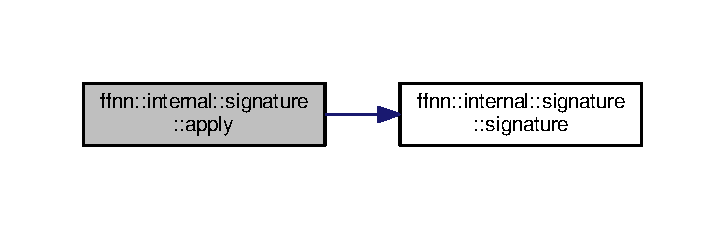
\includegraphics[width=348pt]{namespaceffnn_1_1internal_1_1signature_a6109f0a8c643d2795e9ba2715fe2d684_cgraph}
\end{center}
\end{figure}


\hypertarget{namespaceffnn_1_1internal_1_1signature_a72b327fe2a4910dc1e04a22ba10422b9}{\index{ffnn\-::internal\-::signature@{ffnn\-::internal\-::signature}!check@{check}}
\index{check@{check}!ffnn::internal::signature@{ffnn\-::internal\-::signature}}
\subsubsection[{check}]{\setlength{\rightskip}{0pt plus 5cm}template$<$typename Serializable\-Type , typename Archive $>$ void ffnn\-::internal\-::signature\-::check (
\begin{DoxyParamCaption}
\item[{Archive \&}]{archive}
\end{DoxyParamCaption}
)}}\label{namespaceffnn_1_1internal_1_1signature_a72b327fe2a4910dc1e04a22ba10422b9}


Checks a type signature read from an archive. 


\begin{DoxyParams}[1]{Parameters}
\mbox{\tt in,out}  & {\em archive} & input archive \\
\hline
\end{DoxyParams}


Here is the call graph for this function\-:\nopagebreak
\begin{figure}[H]
\begin{center}
\leavevmode
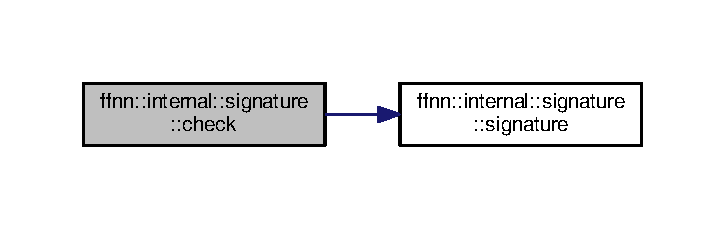
\includegraphics[width=348pt]{namespaceffnn_1_1internal_1_1signature_a72b327fe2a4910dc1e04a22ba10422b9_cgraph}
\end{center}
\end{figure}


\hypertarget{namespaceffnn_1_1internal_1_1signature_a5c9daef9afab6c4cacf3376c2aa3ec13}{\index{ffnn\-::internal\-::signature@{ffnn\-::internal\-::signature}!signature@{signature}}
\index{signature@{signature}!ffnn::internal::signature@{ffnn\-::internal\-::signature}}
\subsubsection[{signature}]{\setlength{\rightskip}{0pt plus 5cm}template$<$typename Type $>$ const std\-::string ffnn\-::internal\-::signature\-::signature (
\begin{DoxyParamCaption}
{}
\end{DoxyParamCaption}
)}}\label{namespaceffnn_1_1internal_1_1signature_a5c9daef9afab6c4cacf3376c2aa3ec13}


Generates a type signature string for a type. 

\begin{DoxyReturn}{Returns}
type signature 
\end{DoxyReturn}
\begin{DoxyNote}{Note}
If using G\-C\-C, the signature will be human-\/readable. 
\end{DoxyNote}


Referenced by apply(), and check().


\hypertarget{namespaceffnn_1_1internal_1_1traits}{\section{ffnn\-:\-:internal\-:\-:traits Namespace Reference}
\label{namespaceffnn_1_1internal_1_1traits}\index{ffnn\-::internal\-::traits@{ffnn\-::internal\-::traits}}
}
\subsection*{Classes}
\begin{DoxyCompactItemize}
\item 
struct \hyperlink{structffnn_1_1internal_1_1traits_1_1is__alignable__128}{is\-\_\-alignable\-\_\-128}
\begin{DoxyCompactList}\small\item\em Has {\ttfamily value\-\_\-type == std\-::true\-\_\-type} if {\ttfamily Object} is a 16-\/byte alignable type. \end{DoxyCompactList}\end{DoxyCompactItemize}

\hypertarget{namespaceffnn_1_1layer}{\section{ffnn\-:\-:layer Namespace Reference}
\label{namespaceffnn_1_1layer}\index{ffnn\-::layer@{ffnn\-::layer}}
}
\subsection*{Namespaces}
\begin{DoxyCompactItemize}
\item 
\hyperlink{namespaceffnn_1_1layer_1_1internal}{internal}
\end{DoxyCompactItemize}
\subsection*{Classes}
\begin{DoxyCompactItemize}
\item 
class \hyperlink{classffnn_1_1layer_1_1_activation}{Activation}
\begin{DoxyCompactList}\small\item\em \hyperlink{classffnn_1_1layer_1_1_activation}{Activation} layer. \end{DoxyCompactList}\item 
class \hyperlink{classffnn_1_1layer_1_1_convolution}{Convolution}
\begin{DoxyCompactList}\small\item\em A convolution layer. \end{DoxyCompactList}\item 
class \hyperlink{classffnn_1_1layer_1_1_filter_bank}{Filter\-Bank}
\item 
class \hyperlink{classffnn_1_1layer_1_1_convolution_volume}{Convolution\-Volume}
\item 
class \hyperlink{classffnn_1_1layer_1_1_fully_connected}{Fully\-Connected}
\begin{DoxyCompactList}\small\item\em A fully-\/connected layer. \end{DoxyCompactList}\item 
class \hyperlink{classffnn_1_1layer_1_1_hidden}{Hidden}
\begin{DoxyCompactList}\small\item\em A network hidden-\/layer object. \end{DoxyCompactList}\item 
class \hyperlink{classffnn_1_1layer_1_1_input}{Input}
\begin{DoxyCompactList}\small\item\em A layer which handles network inputs. \end{DoxyCompactList}\item 
class \hyperlink{classffnn_1_1layer_1_1_layer}{Layer}
\begin{DoxyCompactList}\small\item\em Base object for all layer types. \end{DoxyCompactList}\item 
class \hyperlink{classffnn_1_1layer_1_1_output}{Output}
\begin{DoxyCompactList}\small\item\em A layer which handles network outputs. \end{DoxyCompactList}\item 
class \hyperlink{classffnn_1_1layer_1_1_receptive_volume}{Receptive\-Volume}
\item 
class \hyperlink{classffnn_1_1layer_1_1_sparsely_connected}{Sparsely\-Connected}
\begin{DoxyCompactList}\small\item\em A fully-\/connected layer. \end{DoxyCompactList}\end{DoxyCompactItemize}
\subsection*{Enumerations}
\begin{DoxyCompactItemize}
\item 
enum \hyperlink{namespaceffnn_1_1layer_a254f16beba4fb335d935e9b43bb9e69a}{Embedding\-Mode} \{ \hyperlink{namespaceffnn_1_1layer_a254f16beba4fb335d935e9b43bb9e69aa56bf723aeae4562f2fe05ae5e675da92}{Row\-Embedding} = 0, 
\hyperlink{namespaceffnn_1_1layer_a254f16beba4fb335d935e9b43bb9e69aaede1065f5863208cae7e55561966a182}{Col\-Embedding} = 1, 
\hyperlink{namespaceffnn_1_1layer_a254f16beba4fb335d935e9b43bb9e69aa56bf723aeae4562f2fe05ae5e675da92}{Row\-Embedding} = 0, 
\hyperlink{namespaceffnn_1_1layer_a254f16beba4fb335d935e9b43bb9e69aaede1065f5863208cae7e55561966a182}{Col\-Embedding} = 1
 \}
\item 
enum \hyperlink{namespaceffnn_1_1layer_a254f16beba4fb335d935e9b43bb9e69a}{Embedding\-Mode} \{ \hyperlink{namespaceffnn_1_1layer_a254f16beba4fb335d935e9b43bb9e69aa56bf723aeae4562f2fe05ae5e675da92}{Row\-Embedding} = 0, 
\hyperlink{namespaceffnn_1_1layer_a254f16beba4fb335d935e9b43bb9e69aaede1065f5863208cae7e55561966a182}{Col\-Embedding} = 1, 
\hyperlink{namespaceffnn_1_1layer_a254f16beba4fb335d935e9b43bb9e69aa56bf723aeae4562f2fe05ae5e675da92}{Row\-Embedding} = 0, 
\hyperlink{namespaceffnn_1_1layer_a254f16beba4fb335d935e9b43bb9e69aaede1065f5863208cae7e55561966a182}{Col\-Embedding} = 1
 \}
\end{DoxyCompactItemize}
\subsection*{Functions}
\begin{DoxyCompactItemize}
\item 
{\footnotesize template$<$typename Layer\-Type $>$ }\\bool \hyperlink{namespaceffnn_1_1layer_a33fc9c6c7eb5fbdef14e0aa0db97dd13}{connect} (const typename Layer\-Type\-::\-Ptr \&from, const typename Layer\-Type\-::\-Ptr \&to)
\end{DoxyCompactItemize}


\subsection{Enumeration Type Documentation}
\hypertarget{namespaceffnn_1_1layer_a254f16beba4fb335d935e9b43bb9e69a}{\index{ffnn\-::layer@{ffnn\-::layer}!Embedding\-Mode@{Embedding\-Mode}}
\index{Embedding\-Mode@{Embedding\-Mode}!ffnn::layer@{ffnn\-::layer}}
\subsubsection[{Embedding\-Mode}]{\setlength{\rightskip}{0pt plus 5cm}enum {\bf ffnn\-::layer\-::\-Embedding\-Mode}}}\label{namespaceffnn_1_1layer_a254f16beba4fb335d935e9b43bb9e69a}
\begin{Desc}
\item[Enumerator]\par
\begin{description}
\index{Row\-Embedding@{Row\-Embedding}!ffnn\-::layer@{ffnn\-::layer}}\index{ffnn\-::layer@{ffnn\-::layer}!Row\-Embedding@{Row\-Embedding}}\item[{\em 
\hypertarget{namespaceffnn_1_1layer_a254f16beba4fb335d935e9b43bb9e69aa56bf723aeae4562f2fe05ae5e675da92}{Row\-Embedding}\label{namespaceffnn_1_1layer_a254f16beba4fb335d935e9b43bb9e69aa56bf723aeae4562f2fe05ae5e675da92}
}]Embed depth along filter matrix rows. \index{Col\-Embedding@{Col\-Embedding}!ffnn\-::layer@{ffnn\-::layer}}\index{ffnn\-::layer@{ffnn\-::layer}!Col\-Embedding@{Col\-Embedding}}\item[{\em 
\hypertarget{namespaceffnn_1_1layer_a254f16beba4fb335d935e9b43bb9e69aaede1065f5863208cae7e55561966a182}{Col\-Embedding}\label{namespaceffnn_1_1layer_a254f16beba4fb335d935e9b43bb9e69aaede1065f5863208cae7e55561966a182}
}]Embed depth along filter matrix cols. \index{Row\-Embedding@{Row\-Embedding}!ffnn\-::layer@{ffnn\-::layer}}\index{ffnn\-::layer@{ffnn\-::layer}!Row\-Embedding@{Row\-Embedding}}\item[{\em 
\hypertarget{namespaceffnn_1_1layer_a254f16beba4fb335d935e9b43bb9e69aa56bf723aeae4562f2fe05ae5e675da92}{Row\-Embedding}\label{namespaceffnn_1_1layer_a254f16beba4fb335d935e9b43bb9e69aa56bf723aeae4562f2fe05ae5e675da92}
}]Embed depth along filter matrix rows. \index{Col\-Embedding@{Col\-Embedding}!ffnn\-::layer@{ffnn\-::layer}}\index{ffnn\-::layer@{ffnn\-::layer}!Col\-Embedding@{Col\-Embedding}}\item[{\em 
\hypertarget{namespaceffnn_1_1layer_a254f16beba4fb335d935e9b43bb9e69aaede1065f5863208cae7e55561966a182}{Col\-Embedding}\label{namespaceffnn_1_1layer_a254f16beba4fb335d935e9b43bb9e69aaede1065f5863208cae7e55561966a182}
}]Embed depth along filter matrix cols. \end{description}
\end{Desc}
\hypertarget{namespaceffnn_1_1layer_a254f16beba4fb335d935e9b43bb9e69a}{\index{ffnn\-::layer@{ffnn\-::layer}!Embedding\-Mode@{Embedding\-Mode}}
\index{Embedding\-Mode@{Embedding\-Mode}!ffnn::layer@{ffnn\-::layer}}
\subsubsection[{Embedding\-Mode}]{\setlength{\rightskip}{0pt plus 5cm}enum {\bf ffnn\-::layer\-::\-Embedding\-Mode}}}\label{namespaceffnn_1_1layer_a254f16beba4fb335d935e9b43bb9e69a}
\begin{Desc}
\item[Enumerator]\par
\begin{description}
\index{Row\-Embedding@{Row\-Embedding}!ffnn\-::layer@{ffnn\-::layer}}\index{ffnn\-::layer@{ffnn\-::layer}!Row\-Embedding@{Row\-Embedding}}\item[{\em 
\hypertarget{namespaceffnn_1_1layer_a254f16beba4fb335d935e9b43bb9e69aa56bf723aeae4562f2fe05ae5e675da92}{Row\-Embedding}\label{namespaceffnn_1_1layer_a254f16beba4fb335d935e9b43bb9e69aa56bf723aeae4562f2fe05ae5e675da92}
}]Embed depth along filter matrix rows. \index{Col\-Embedding@{Col\-Embedding}!ffnn\-::layer@{ffnn\-::layer}}\index{ffnn\-::layer@{ffnn\-::layer}!Col\-Embedding@{Col\-Embedding}}\item[{\em 
\hypertarget{namespaceffnn_1_1layer_a254f16beba4fb335d935e9b43bb9e69aaede1065f5863208cae7e55561966a182}{Col\-Embedding}\label{namespaceffnn_1_1layer_a254f16beba4fb335d935e9b43bb9e69aaede1065f5863208cae7e55561966a182}
}]Embed depth along filter matrix cols. \index{Row\-Embedding@{Row\-Embedding}!ffnn\-::layer@{ffnn\-::layer}}\index{ffnn\-::layer@{ffnn\-::layer}!Row\-Embedding@{Row\-Embedding}}\item[{\em 
\hypertarget{namespaceffnn_1_1layer_a254f16beba4fb335d935e9b43bb9e69aa56bf723aeae4562f2fe05ae5e675da92}{Row\-Embedding}\label{namespaceffnn_1_1layer_a254f16beba4fb335d935e9b43bb9e69aa56bf723aeae4562f2fe05ae5e675da92}
}]Embed depth along filter matrix rows. \index{Col\-Embedding@{Col\-Embedding}!ffnn\-::layer@{ffnn\-::layer}}\index{ffnn\-::layer@{ffnn\-::layer}!Col\-Embedding@{Col\-Embedding}}\item[{\em 
\hypertarget{namespaceffnn_1_1layer_a254f16beba4fb335d935e9b43bb9e69aaede1065f5863208cae7e55561966a182}{Col\-Embedding}\label{namespaceffnn_1_1layer_a254f16beba4fb335d935e9b43bb9e69aaede1065f5863208cae7e55561966a182}
}]Embed depth along filter matrix cols. \end{description}
\end{Desc}


\subsection{Function Documentation}
\hypertarget{namespaceffnn_1_1layer_a33fc9c6c7eb5fbdef14e0aa0db97dd13}{\index{ffnn\-::layer@{ffnn\-::layer}!connect@{connect}}
\index{connect@{connect}!ffnn::layer@{ffnn\-::layer}}
\subsubsection[{connect}]{\setlength{\rightskip}{0pt plus 5cm}template$<$typename Layer\-Type $>$ bool ffnn\-::layer\-::connect (
\begin{DoxyParamCaption}
\item[{const typename Layer\-Type\-::\-Ptr \&}]{from, }
\item[{const typename Layer\-Type\-::\-Ptr \&}]{to}
\end{DoxyParamCaption}
)}}\label{namespaceffnn_1_1layer_a33fc9c6c7eb5fbdef14e0aa0db97dd13}

\hypertarget{namespaceffnn_1_1layer_1_1convolution}{\section{ffnn\-:\-:layer\-:\-:convolution Namespace Reference}
\label{namespaceffnn_1_1layer_1_1convolution}\index{ffnn\-::layer\-::convolution@{ffnn\-::layer\-::convolution}}
}
\subsection*{Namespaces}
\begin{DoxyCompactItemize}
\item 
\hyperlink{namespaceffnn_1_1layer_1_1convolution_1_1filter}{filter}
\end{DoxyCompactItemize}
\subsection*{Classes}
\begin{DoxyCompactItemize}
\item 
struct \hyperlink{structffnn_1_1layer_1_1convolution_1_1options}{options}
\begin{DoxyCompactList}\small\item\em Describes compile-\/time options used to set up a \hyperlink{classffnn_1_1layer_1_1_convolution}{Convolution} object. \end{DoxyCompactList}\item 
struct \hyperlink{structffnn_1_1layer_1_1convolution_1_1extrinsics}{extrinsics}
\begin{DoxyCompactList}\small\item\em Describes types based on compile-\/time options. \end{DoxyCompactList}\item 
class \hyperlink{classffnn_1_1layer_1_1convolution_1_1_configuration}{Configuration}
\begin{DoxyCompactList}\small\item\em \hyperlink{classffnn_1_1layer_1_1_layer}{Layer} configuration struct. \end{DoxyCompactList}\item 
class \hyperlink{classffnn_1_1layer_1_1convolution_1_1_filter}{Filter}
\begin{DoxyCompactList}\small\item\em \hyperlink{classffnn_1_1layer_1_1convolution_1_1_filter}{Filter} parameters to be use with a \hyperlink{classffnn_1_1layer_1_1_convolution}{Convolution} layer. \end{DoxyCompactList}\end{DoxyCompactItemize}
\subsection*{Enumerations}
\begin{DoxyCompactItemize}
\item 
enum \hyperlink{namespaceffnn_1_1layer_1_1convolution_ad420d4eb8edd7c254d1f0aaaad81017f}{Embedding\-Mode} \{ \hyperlink{namespaceffnn_1_1layer_1_1convolution_ad420d4eb8edd7c254d1f0aaaad81017fa1c03b5145e31615496457aa687a180c2}{Row\-Embedding} = 0, 
\hyperlink{namespaceffnn_1_1layer_1_1convolution_ad420d4eb8edd7c254d1f0aaaad81017fae2ba27e8fa1aed3f003e54947f37d17e}{Col\-Embedding} = 1
 \}
\begin{DoxyCompactList}\small\item\em Used to select how depth of an input/outut volume is embedded in matrix form. \end{DoxyCompactList}\end{DoxyCompactItemize}
\subsection*{Functions}
\begin{DoxyCompactItemize}
\item 
{\footnotesize template$<$Embedding\-Mode mode, Embedding\-Mode ref, typename Size\-Type $>$ }\\constexpr Size\-Type \hyperlink{namespaceffnn_1_1layer_1_1convolution_a0cca23056b3d9d79e6604c9419814351}{embed\-\_\-dimension} (Size\-Type n, Size\-Type m)
\begin{DoxyCompactList}\small\item\em Selects size or depth-\/embedded size based on embedding mode. \end{DoxyCompactList}\item 
{\footnotesize template$<$Embedding\-Mode mode$>$ }\\constexpr int \hyperlink{namespaceffnn_1_1layer_1_1convolution_a88d0a4ec4a7dbc89c35ce95d859a78cf}{embed\-\_\-data\-\_\-order} ()
\begin{DoxyCompactList}\small\item\em Selects data ordering based on embedding mode. \end{DoxyCompactList}\item 
{\footnotesize template$<$Embedding\-Mode mode, typename Shape\-Type $>$ }\\Shape\-Type \hyperlink{namespaceffnn_1_1layer_1_1convolution_a773c97d21219b026d77a46ac642ef4e6}{embed\-\_\-shape\-\_\-transform} (const Shape\-Type \&shape)
\begin{DoxyCompactList}\small\item\em Transforms shape dimensions to a depth-\/embedded representation. \end{DoxyCompactList}\item 
{\footnotesize template$<$typename Size\-Type $>$ }\\constexpr Size\-Type \hyperlink{namespaceffnn_1_1layer_1_1convolution_aca263840b789df041d868a8a87dbf36a}{output\-\_\-dimension} (Size\-Type n, Size\-Type fn, Size\-Type stride)
\begin{DoxyCompactList}\small\item\em Computes convolution output size. \end{DoxyCompactList}\end{DoxyCompactItemize}


\subsection{Enumeration Type Documentation}
\hypertarget{namespaceffnn_1_1layer_1_1convolution_ad420d4eb8edd7c254d1f0aaaad81017f}{\index{ffnn\-::layer\-::convolution@{ffnn\-::layer\-::convolution}!Embedding\-Mode@{Embedding\-Mode}}
\index{Embedding\-Mode@{Embedding\-Mode}!ffnn::layer::convolution@{ffnn\-::layer\-::convolution}}
\subsubsection[{Embedding\-Mode}]{\setlength{\rightskip}{0pt plus 5cm}enum {\bf ffnn\-::layer\-::convolution\-::\-Embedding\-Mode}}}\label{namespaceffnn_1_1layer_1_1convolution_ad420d4eb8edd7c254d1f0aaaad81017f}


Used to select how depth of an input/outut volume is embedded in matrix form. 

\begin{DoxyNote}{Note}
{\ttfamily Row\-Embedding} generally implies that the underly matrix will have row-\/major ordering. This is because of how this data is usually accessed 

{\ttfamily Col\-Embedding} generally implies that the underly matrix will have collumn-\/major ordering. This is because of how this data is usually accessed 
\end{DoxyNote}
\begin{Desc}
\item[Enumerator]\par
\begin{description}
\index{Row\-Embedding@{Row\-Embedding}!ffnn\-::layer\-::convolution@{ffnn\-::layer\-::convolution}}\index{ffnn\-::layer\-::convolution@{ffnn\-::layer\-::convolution}!Row\-Embedding@{Row\-Embedding}}\item[{\em 
\hypertarget{namespaceffnn_1_1layer_1_1convolution_ad420d4eb8edd7c254d1f0aaaad81017fa1c03b5145e31615496457aa687a180c2}{Row\-Embedding}\label{namespaceffnn_1_1layer_1_1convolution_ad420d4eb8edd7c254d1f0aaaad81017fa1c03b5145e31615496457aa687a180c2}
}]Embed depth along filter matrix rows. \index{Col\-Embedding@{Col\-Embedding}!ffnn\-::layer\-::convolution@{ffnn\-::layer\-::convolution}}\index{ffnn\-::layer\-::convolution@{ffnn\-::layer\-::convolution}!Col\-Embedding@{Col\-Embedding}}\item[{\em 
\hypertarget{namespaceffnn_1_1layer_1_1convolution_ad420d4eb8edd7c254d1f0aaaad81017fae2ba27e8fa1aed3f003e54947f37d17e}{Col\-Embedding}\label{namespaceffnn_1_1layer_1_1convolution_ad420d4eb8edd7c254d1f0aaaad81017fae2ba27e8fa1aed3f003e54947f37d17e}
}]Embed depth along filter matrix cols. \end{description}
\end{Desc}


\subsection{Function Documentation}
\hypertarget{namespaceffnn_1_1layer_1_1convolution_a88d0a4ec4a7dbc89c35ce95d859a78cf}{\index{ffnn\-::layer\-::convolution@{ffnn\-::layer\-::convolution}!embed\-\_\-data\-\_\-order@{embed\-\_\-data\-\_\-order}}
\index{embed\-\_\-data\-\_\-order@{embed\-\_\-data\-\_\-order}!ffnn::layer::convolution@{ffnn\-::layer\-::convolution}}
\subsubsection[{embed\-\_\-data\-\_\-order}]{\setlength{\rightskip}{0pt plus 5cm}template$<$Embedding\-Mode mode$>$ constexpr int ffnn\-::layer\-::convolution\-::embed\-\_\-data\-\_\-order (
\begin{DoxyParamCaption}
{}
\end{DoxyParamCaption}
)}}\label{namespaceffnn_1_1layer_1_1convolution_a88d0a4ec4a7dbc89c35ce95d859a78cf}


Selects data ordering based on embedding mode. 


\begin{DoxyRetVals}{Return values}
{\em $<$code$>$\-Eigen\-::\-Col\-Major$<$/code$>$} & if {\ttfamily Embedding\-Mode == Col\-Embedding} \\
\hline
{\em $<$code$>$\-Eigen\-::\-Row\-Major$<$/code$>$} & if {\ttfamily Embedding\-Mode == Row\-Embedding} \\
\hline
\end{DoxyRetVals}
\hypertarget{namespaceffnn_1_1layer_1_1convolution_a0cca23056b3d9d79e6604c9419814351}{\index{ffnn\-::layer\-::convolution@{ffnn\-::layer\-::convolution}!embed\-\_\-dimension@{embed\-\_\-dimension}}
\index{embed\-\_\-dimension@{embed\-\_\-dimension}!ffnn::layer::convolution@{ffnn\-::layer\-::convolution}}
\subsubsection[{embed\-\_\-dimension}]{\setlength{\rightskip}{0pt plus 5cm}template$<$Embedding\-Mode mode, Embedding\-Mode ref, typename Size\-Type $>$ constexpr Size\-Type ffnn\-::layer\-::convolution\-::embed\-\_\-dimension (
\begin{DoxyParamCaption}
\item[{Size\-Type}]{n, }
\item[{Size\-Type}]{m}
\end{DoxyParamCaption}
)}}\label{namespaceffnn_1_1layer_1_1convolution_a0cca23056b3d9d79e6604c9419814351}


Selects size or depth-\/embedded size based on embedding mode. 


\begin{DoxyParams}{Parameters}
{\em n} & interger dimension \\
\hline
{\em m} & interger dimension \\
\hline
\end{DoxyParams}

\begin{DoxyRetVals}{Return values}
{\em (n$\ast$m)} & if (mode == ref) and sizes are not dynamic \\
\hline
{\em n} & if (mode != ref) \\
\hline
\end{DoxyRetVals}
\hypertarget{namespaceffnn_1_1layer_1_1convolution_a773c97d21219b026d77a46ac642ef4e6}{\index{ffnn\-::layer\-::convolution@{ffnn\-::layer\-::convolution}!embed\-\_\-shape\-\_\-transform@{embed\-\_\-shape\-\_\-transform}}
\index{embed\-\_\-shape\-\_\-transform@{embed\-\_\-shape\-\_\-transform}!ffnn::layer::convolution@{ffnn\-::layer\-::convolution}}
\subsubsection[{embed\-\_\-shape\-\_\-transform}]{\setlength{\rightskip}{0pt plus 5cm}template$<$Embedding\-Mode mode, typename Shape\-Type $>$ Shape\-Type ffnn\-::layer\-::convolution\-::embed\-\_\-shape\-\_\-transform (
\begin{DoxyParamCaption}
\item[{const Shape\-Type \&}]{shape}
\end{DoxyParamCaption}
)}}\label{namespaceffnn_1_1layer_1_1convolution_a773c97d21219b026d77a46ac642ef4e6}


Transforms shape dimensions to a depth-\/embedded representation. 


\begin{DoxyParams}{Parameters}
{\em shape} & original shape repsentation \\
\hline
\end{DoxyParams}
\begin{DoxyReturn}{Returns}
depth-\/embedded version of shape 
\end{DoxyReturn}
\hypertarget{namespaceffnn_1_1layer_1_1convolution_aca263840b789df041d868a8a87dbf36a}{\index{ffnn\-::layer\-::convolution@{ffnn\-::layer\-::convolution}!output\-\_\-dimension@{output\-\_\-dimension}}
\index{output\-\_\-dimension@{output\-\_\-dimension}!ffnn::layer::convolution@{ffnn\-::layer\-::convolution}}
\subsubsection[{output\-\_\-dimension}]{\setlength{\rightskip}{0pt plus 5cm}template$<$typename Size\-Type $>$ constexpr Size\-Type ffnn\-::layer\-::convolution\-::output\-\_\-dimension (
\begin{DoxyParamCaption}
\item[{Size\-Type}]{n, }
\item[{Size\-Type}]{fn, }
\item[{Size\-Type}]{stride}
\end{DoxyParamCaption}
)}}\label{namespaceffnn_1_1layer_1_1convolution_aca263840b789df041d868a8a87dbf36a}


Computes convolution output size. 


\begin{DoxyParams}{Parameters}
{\em n} & convolution input layer dimension \\
\hline
{\em fn} & filter dimension \\
\hline
{\em stide} & filter stride \\
\hline
\end{DoxyParams}

\begin{DoxyRetVals}{Return values}
{\em size} & if sizes are not dynamic \\
\hline
\end{DoxyRetVals}

\hypertarget{namespaceffnn_1_1layer_1_1convolution_1_1filter}{\section{ffnn\-:\-:layer\-:\-:convolution\-:\-:filter Namespace Reference}
\label{namespaceffnn_1_1layer_1_1convolution_1_1filter}\index{ffnn\-::layer\-::convolution\-::filter@{ffnn\-::layer\-::convolution\-::filter}}
}
\subsection*{Classes}
\begin{DoxyCompactItemize}
\item 
struct \hyperlink{structffnn_1_1layer_1_1convolution_1_1filter_1_1options}{options}
\begin{DoxyCompactList}\small\item\em Describes compile-\/time options and extrinsic parameters used to set up a \hyperlink{structffnn_1_1layer_1_1convolution_1_1_filter}{Filter} object. \end{DoxyCompactList}\item 
struct \hyperlink{structffnn_1_1layer_1_1convolution_1_1filter_1_1extrinsics}{extrinsics}
\begin{DoxyCompactList}\small\item\em Describes types based on compile-\/time options. \end{DoxyCompactList}\end{DoxyCompactItemize}

\hypertarget{namespaceffnn_1_1layer_1_1hidden}{\section{ffnn\-:\-:layer\-:\-:hidden Namespace Reference}
\label{namespaceffnn_1_1layer_1_1hidden}\index{ffnn\-::layer\-::hidden@{ffnn\-::layer\-::hidden}}
}
\subsection*{Classes}
\begin{DoxyCompactItemize}
\item 
struct \hyperlink{structffnn_1_1layer_1_1hidden_1_1options}{options}
\begin{DoxyCompactList}\small\item\em Describes compile-\/time options used to set up a \hyperlink{classffnn_1_1layer_1_1_convolution}{Convolution} object. \end{DoxyCompactList}\item 
struct \hyperlink{structffnn_1_1layer_1_1hidden_1_1extrinsics}{extrinsics}
\begin{DoxyCompactList}\small\item\em Describes types based on compile-\/time options. \end{DoxyCompactList}\end{DoxyCompactItemize}

\hypertarget{namespaceffnn_1_1logging}{\section{ffnn\-:\-:logging Namespace Reference}
\label{namespaceffnn_1_1logging}\index{ffnn\-::logging@{ffnn\-::logging}}
}
\subsection*{Variables}
\begin{DoxyCompactItemize}
\item 
const char $\ast$ \hyperlink{group___unicode_color_definitions_ga65590452b7707feb609f43a9ca306d42}{H\-E\-A\-D\-E\-R} = \char`\"{}\textbackslash{}033\mbox{[}95m\char`\"{}
\item 
const char $\ast$ \hyperlink{group___unicode_color_definitions_ga359f39576675d57a59f93e2addae319a}{D\-E\-B\-U\-G} = \char`\"{}\textbackslash{}033\mbox{[}94m\char`\"{}
\item 
const char $\ast$ \hyperlink{group___unicode_color_definitions_gab5d57e4b1db90e208ccad18ce1b0f836}{I\-N\-F\-O} = \char`\"{}\textbackslash{}033\mbox{[}92m\char`\"{}
\item 
const char $\ast$ \hyperlink{group___unicode_color_definitions_gafc935a693ebe97569c82dd2415bb7373}{W\-A\-R\-N} = \char`\"{}\textbackslash{}033\mbox{[}93m\char`\"{}
\item 
const char $\ast$ \hyperlink{group___unicode_color_definitions_ga10413caefeb3f647a80cfdb9d1874276}{I\-N\-T\-E\-R\-N\-A\-L} = \char`\"{}\textbackslash{}033\mbox{[}96m\char`\"{}
\item 
const char $\ast$ \hyperlink{group___unicode_color_definitions_ga2047db0e31e0a45c7c213845567afc06}{F\-A\-I\-L} = \char`\"{}\textbackslash{}033\mbox{[}91m\char`\"{}
\item 
const char $\ast$ \hyperlink{group___unicode_color_definitions_gab21e47dcbc216f8fc7de88bd217f9f0a}{E\-N\-D\-C} = \char`\"{}\textbackslash{}033\mbox{[}0m\char`\"{}
\item 
const char $\ast$ \hyperlink{group___unicode_color_definitions_ga32fca3fc24af93ce9c4ca33b4a6a3dde}{B\-O\-L\-D} = \char`\"{}\textbackslash{}033\mbox{[}1m\char`\"{}
\item 
const char $\ast$ \hyperlink{group___unicode_color_definitions_gab2b4d719c3fe8672abf96e00a37c799c}{U\-N\-D\-E\-R\-L\-I\-N\-E} = \char`\"{}\textbackslash{}033\mbox{[}4m\char`\"{}
\end{DoxyCompactItemize}

\hypertarget{namespaceffnn_1_1neuron}{\section{ffnn\-:\-:neuron Namespace Reference}
\label{namespaceffnn_1_1neuron}\index{ffnn\-::neuron@{ffnn\-::neuron}}
}
\subsection*{Namespaces}
\begin{DoxyCompactItemize}
\item 
\hyperlink{namespaceffnn_1_1neuron_1_1modifier}{modifier}
\end{DoxyCompactItemize}
\subsection*{Classes}
\begin{DoxyCompactItemize}
\item 
class \hyperlink{classffnn_1_1neuron_1_1_leaky_rectified_linear}{Leaky\-Rectified\-Linear}
\begin{DoxyCompactList}\small\item\em A leaky-\/rectified linear activation unit. \end{DoxyCompactList}\item 
class \hyperlink{classffnn_1_1neuron_1_1_le_cun_sigmoid}{Le\-Cun\-Sigmoid}
\begin{DoxyCompactList}\small\item\em A bipolar sigmoid activation unit scaled to prevent saturation. \end{DoxyCompactList}\item 
class \hyperlink{classffnn_1_1neuron_1_1_linear}{Linear}
\begin{DoxyCompactList}\small\item\em A linear activation unit. \end{DoxyCompactList}\item 
struct \hyperlink{structffnn_1_1neuron_1_1is__neuron}{is\-\_\-neuron}
\item 
class \hyperlink{classffnn_1_1neuron_1_1_neuron}{Neuron}
\begin{DoxyCompactList}\small\item\em A basic activation unit type. \end{DoxyCompactList}\item 
class \hyperlink{classffnn_1_1neuron_1_1_rectified_linear}{Rectified\-Linear}
\begin{DoxyCompactList}\small\item\em A rectified linear activation unit. \end{DoxyCompactList}\item 
class \hyperlink{classffnn_1_1neuron_1_1_sigmoid}{Sigmoid}
\begin{DoxyCompactList}\small\item\em A bipolar sigmoid activation unit. \end{DoxyCompactList}\item 
class \hyperlink{classffnn_1_1neuron_1_1_soft_sign}{Soft\-Sign}
\begin{DoxyCompactList}\small\item\em A soft-\/sign activation unit. \end{DoxyCompactList}\end{DoxyCompactItemize}

\hypertarget{namespaceffnn_1_1neuron_1_1modifier}{\section{ffnn\-:\-:neuron\-:\-:modifier Namespace Reference}
\label{namespaceffnn_1_1neuron_1_1modifier}\index{ffnn\-::neuron\-::modifier@{ffnn\-::neuron\-::modifier}}
}
\subsection*{Classes}
\begin{DoxyCompactItemize}
\item 
class \hyperlink{classffnn_1_1neuron_1_1modifier_1_1_dropout}{Dropout}
\item 
class \hyperlink{classffnn_1_1neuron_1_1modifier_1_1_soft_dropout}{Soft\-Dropout}
\end{DoxyCompactItemize}

\hypertarget{namespaceffnn_1_1optimizer}{\section{ffnn\-:\-:optimizer Namespace Reference}
\label{namespaceffnn_1_1optimizer}\index{ffnn\-::optimizer@{ffnn\-::optimizer}}
}
\subsection*{Classes}
\begin{DoxyCompactItemize}
\item 
class \hyperlink{classffnn_1_1optimizer_1_1_adam_states}{Adam\-States}
\item 
class \hyperlink{classffnn_1_1optimizer_1_1_adam_3_01layer_1_1_fully_connected_3_01_value_type_00_01_inputs_at_co08ce471fd3ee7441a350cc42cfd35bcd}{Adam$<$ layer\-::\-Fully\-Connected$<$ Value\-Type, Inputs\-At\-Compile\-Time, Outputs\-At\-Compile\-Time $>$ $>$}
\item 
class \hyperlink{classffnn_1_1optimizer_1_1_gradient_descent_3_01layer_1_1_convolution_3_01_t_a_r_g_s_01_4_01_4}{Gradient\-Descent$<$ layer\-::\-Convolution$<$ T\-A\-R\-G\-S $>$ $>$}
\item 
class \hyperlink{classffnn_1_1optimizer_1_1_gradient_descent_3_01layer_1_1_fully_connected_3_01_value_type_00_01_5467194c2be34d4b726502ad96dff6d3}{Gradient\-Descent$<$ layer\-::\-Fully\-Connected$<$ Value\-Type, Options, Extrinsics $>$, Cross\-Entropy $>$}
\item 
class \hyperlink{classffnn_1_1optimizer_1_1_none}{None}
\item 
class \hyperlink{classffnn_1_1optimizer_1_1_adam}{Adam}
\item 
class \hyperlink{classffnn_1_1optimizer_1_1_gradient_descent}{Gradient\-Descent}
\item 
class \hyperlink{classffnn_1_1optimizer_1_1_gradient_descent__}{Gradient\-Descent\-\_\-}
\item 
class \hyperlink{classffnn_1_1optimizer_1_1_optimizer}{Optimizer}
\begin{DoxyCompactList}\small\item\em A layer-\/wise optimizer visitor. \end{DoxyCompactList}\end{DoxyCompactItemize}
\subsection*{Enumerations}
\begin{DoxyCompactItemize}
\item 
enum \hyperlink{namespaceffnn_1_1optimizer_a9a8fe8c3d1a3a20231195d767fbf65fa}{Loss\-Function} \{ \\*
\hyperlink{namespaceffnn_1_1optimizer_a9a8fe8c3d1a3a20231195d767fbf65faaa0598d50e766937658e2677d13e574f8}{Cross\-Entropy}, 
\hyperlink{namespaceffnn_1_1optimizer_a9a8fe8c3d1a3a20231195d767fbf65faaeb6fd7c27abcc8aaf97be3622c44ce4b}{L2}, 
\hyperlink{namespaceffnn_1_1optimizer_a9a8fe8c3d1a3a20231195d767fbf65faadb600e39bd84006159541fa0cd788cc9}{L1}, 
\hyperlink{namespaceffnn_1_1optimizer_a9a8fe8c3d1a3a20231195d767fbf65faafda22da78e671e6ea3845179b756aed6}{Logistic}, 
\\*
\hyperlink{namespaceffnn_1_1optimizer_a9a8fe8c3d1a3a20231195d767fbf65faa9a2f9c7afed39162a2b1c13936e8b266}{Hinge}, 
\hyperlink{namespaceffnn_1_1optimizer_a9a8fe8c3d1a3a20231195d767fbf65faa912c1f6b00a2fbbae2d62b7f791a9ff4}{Exponential}
 \}
\begin{DoxyCompactList}\small\item\em Loss-\/function enumerations. \end{DoxyCompactList}\end{DoxyCompactItemize}


\subsection{Enumeration Type Documentation}
\hypertarget{namespaceffnn_1_1optimizer_a9a8fe8c3d1a3a20231195d767fbf65fa}{\index{ffnn\-::optimizer@{ffnn\-::optimizer}!Loss\-Function@{Loss\-Function}}
\index{Loss\-Function@{Loss\-Function}!ffnn::optimizer@{ffnn\-::optimizer}}
\subsubsection[{Loss\-Function}]{\setlength{\rightskip}{0pt plus 5cm}enum {\bf ffnn\-::optimizer\-::\-Loss\-Function}}}\label{namespaceffnn_1_1optimizer_a9a8fe8c3d1a3a20231195d767fbf65fa}


Loss-\/function enumerations. 

\begin{Desc}
\item[Enumerator]\par
\begin{description}
\index{Cross\-Entropy@{Cross\-Entropy}!ffnn\-::optimizer@{ffnn\-::optimizer}}\index{ffnn\-::optimizer@{ffnn\-::optimizer}!Cross\-Entropy@{Cross\-Entropy}}\item[{\em 
\hypertarget{namespaceffnn_1_1optimizer_a9a8fe8c3d1a3a20231195d767fbf65faaa0598d50e766937658e2677d13e574f8}{Cross\-Entropy}\label{namespaceffnn_1_1optimizer_a9a8fe8c3d1a3a20231195d767fbf65faaa0598d50e766937658e2677d13e574f8}
}]\index{L2@{L2}!ffnn\-::optimizer@{ffnn\-::optimizer}}\index{ffnn\-::optimizer@{ffnn\-::optimizer}!L2@{L2}}\item[{\em 
\hypertarget{namespaceffnn_1_1optimizer_a9a8fe8c3d1a3a20231195d767fbf65faaeb6fd7c27abcc8aaf97be3622c44ce4b}{L2}\label{namespaceffnn_1_1optimizer_a9a8fe8c3d1a3a20231195d767fbf65faaeb6fd7c27abcc8aaf97be3622c44ce4b}
}]\index{L1@{L1}!ffnn\-::optimizer@{ffnn\-::optimizer}}\index{ffnn\-::optimizer@{ffnn\-::optimizer}!L1@{L1}}\item[{\em 
\hypertarget{namespaceffnn_1_1optimizer_a9a8fe8c3d1a3a20231195d767fbf65faadb600e39bd84006159541fa0cd788cc9}{L1}\label{namespaceffnn_1_1optimizer_a9a8fe8c3d1a3a20231195d767fbf65faadb600e39bd84006159541fa0cd788cc9}
}]\index{Logistic@{Logistic}!ffnn\-::optimizer@{ffnn\-::optimizer}}\index{ffnn\-::optimizer@{ffnn\-::optimizer}!Logistic@{Logistic}}\item[{\em 
\hypertarget{namespaceffnn_1_1optimizer_a9a8fe8c3d1a3a20231195d767fbf65faafda22da78e671e6ea3845179b756aed6}{Logistic}\label{namespaceffnn_1_1optimizer_a9a8fe8c3d1a3a20231195d767fbf65faafda22da78e671e6ea3845179b756aed6}
}]\index{Hinge@{Hinge}!ffnn\-::optimizer@{ffnn\-::optimizer}}\index{ffnn\-::optimizer@{ffnn\-::optimizer}!Hinge@{Hinge}}\item[{\em 
\hypertarget{namespaceffnn_1_1optimizer_a9a8fe8c3d1a3a20231195d767fbf65faa9a2f9c7afed39162a2b1c13936e8b266}{Hinge}\label{namespaceffnn_1_1optimizer_a9a8fe8c3d1a3a20231195d767fbf65faa9a2f9c7afed39162a2b1c13936e8b266}
}]\index{Exponential@{Exponential}!ffnn\-::optimizer@{ffnn\-::optimizer}}\index{ffnn\-::optimizer@{ffnn\-::optimizer}!Exponential@{Exponential}}\item[{\em 
\hypertarget{namespaceffnn_1_1optimizer_a9a8fe8c3d1a3a20231195d767fbf65faa912c1f6b00a2fbbae2d62b7f791a9ff4}{Exponential}\label{namespaceffnn_1_1optimizer_a9a8fe8c3d1a3a20231195d767fbf65faa912c1f6b00a2fbbae2d62b7f791a9ff4}
}]\end{description}
\end{Desc}

\chapter{Class Documentation}
\hypertarget{classffnn_1_1layer_1_1_activation}{\section{ffnn\-:\-:layer\-:\-:Activation$<$ Value\-Type, Neuron\-Type, Size\-At\-Compile\-Time $>$ Class Template Reference}
\label{classffnn_1_1layer_1_1_activation}\index{ffnn\-::layer\-::\-Activation$<$ Value\-Type, Neuron\-Type, Size\-At\-Compile\-Time $>$@{ffnn\-::layer\-::\-Activation$<$ Value\-Type, Neuron\-Type, Size\-At\-Compile\-Time $>$}}
}


\hyperlink{classffnn_1_1layer_1_1_activation}{Activation} layer.  




{\ttfamily \#include \char`\"{}activation.\-h\char`\"{}}



Inheritance diagram for ffnn\-:\-:layer\-:\-:Activation$<$ Value\-Type, Neuron\-Type, Size\-At\-Compile\-Time $>$\-:
\nopagebreak
\begin{figure}[H]
\begin{center}
\leavevmode
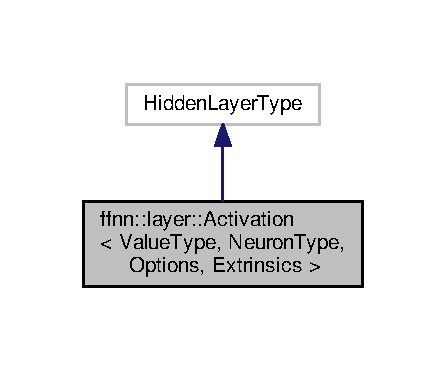
\includegraphics[width=242pt]{classffnn_1_1layer_1_1_activation__inherit__graph}
\end{center}
\end{figure}


Collaboration diagram for ffnn\-:\-:layer\-:\-:Activation$<$ Value\-Type, Neuron\-Type, Size\-At\-Compile\-Time $>$\-:
\nopagebreak
\begin{figure}[H]
\begin{center}
\leavevmode
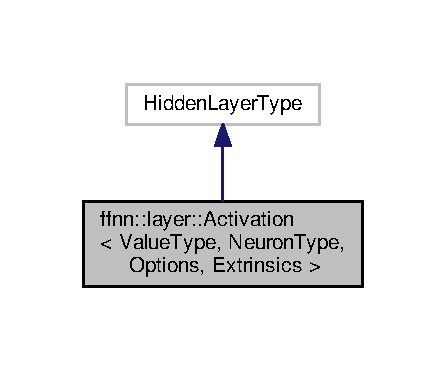
\includegraphics[width=242pt]{classffnn_1_1layer_1_1_activation__coll__graph}
\end{center}
\end{figure}
\subsection*{Public Types}
\begin{DoxyCompactItemize}
\item 
using \hyperlink{classffnn_1_1layer_1_1_activation_a201ec82cc70826c458c1f4dc5e7f3fdf}{Base} = \hyperlink{classffnn_1_1layer_1_1_hidden}{Hidden}$<$ Value\-Type, Size\-At\-Compile\-Time, 1, Size\-At\-Compile\-Time, 1 $>$
\begin{DoxyCompactList}\small\item\em Base type alias. \end{DoxyCompactList}\item 
typedef \hyperlink{classffnn_1_1layer_1_1internal_1_1_interface_a7f834e3365e5199bcbcd16d9abd63941}{Base\-::\-Scalar\-Type} \hyperlink{classffnn_1_1layer_1_1_activation_ad864a6480079601f9723311a686550c3}{Scalar\-Type}
\begin{DoxyCompactList}\small\item\em Scalar type standardization. \end{DoxyCompactList}\item 
typedef \hyperlink{classffnn_1_1layer_1_1_hidden_a3deb1dc4b3a83b3d6749474debee025f}{Base\-::\-Size\-Type} \hyperlink{classffnn_1_1layer_1_1_activation_ab3635bf431b97e8f1b51704f20d60d34}{Size\-Type}
\begin{DoxyCompactList}\small\item\em Size type standardization. \end{DoxyCompactList}\item 
typedef \hyperlink{classffnn_1_1layer_1_1_hidden_a4a191bc002b2545231a3d80c99004693}{Base\-::\-Offset\-Type} \hyperlink{classffnn_1_1layer_1_1_activation_aff203e6e98860cf5887ecc18894619fb}{Offset\-Type}
\begin{DoxyCompactList}\small\item\em Offset type standardization. \end{DoxyCompactList}\end{DoxyCompactItemize}
\subsection*{Public Member Functions}
\begin{DoxyCompactItemize}
\item 
\hyperlink{classffnn_1_1layer_1_1_activation_a433d57370b979f91679e2065c48663f9}{Activation} ()
\begin{DoxyCompactList}\small\item\em Default constructor. \end{DoxyCompactList}\item 
virtual \hyperlink{classffnn_1_1layer_1_1_activation_a4b353acb2031fff2e7a15cf0895d346d}{$\sim$\-Activation} ()
\item 
virtual bool \hyperlink{classffnn_1_1layer_1_1_activation_ae73ef2d36d9c5ce3c219f6a51cba3c35}{initialize} ()
\begin{DoxyCompactList}\small\item\em Initialize the layer. \end{DoxyCompactList}\item 
virtual bool \hyperlink{classffnn_1_1layer_1_1_activation_aa7f88c8bc20589dc51d9dd615b8c4580}{forward} ()
\begin{DoxyCompactList}\small\item\em Forward value propagation. \end{DoxyCompactList}\item 
virtual bool \hyperlink{classffnn_1_1layer_1_1_activation_a3c4284245343f2132dd28eaf7ffbed47}{backward} ()
\begin{DoxyCompactList}\small\item\em Performs backward error propagation. \end{DoxyCompactList}\end{DoxyCompactItemize}
\subsection*{Protected Member Functions}
\begin{DoxyCompactItemize}
\item 
void \hyperlink{classffnn_1_1layer_1_1_activation_ab5525e49c08fc593856b9c95e0eba1ee}{save} (\hyperlink{classffnn_1_1traits_1_1_serializable_a08d986df75d363fa79506d4f6045cb9f}{Output\-Archive} \&ar, \hyperlink{classffnn_1_1traits_1_1_serializable_a08924b3b7d20cb3cb6eafe517d4f7b30}{Version\-Type} version) const 
\begin{DoxyCompactList}\small\item\em Save serializer. \end{DoxyCompactList}\item 
void \hyperlink{classffnn_1_1layer_1_1_activation_a045ecc330b67cdc3a41d6d7fc3a8dbf2}{load} (\hyperlink{classffnn_1_1traits_1_1_serializable_a6e626759259f8f370dd4303b4441a234}{Input\-Archive} \&ar, \hyperlink{classffnn_1_1traits_1_1_serializable_a08924b3b7d20cb3cb6eafe517d4f7b30}{Version\-Type} version)
\begin{DoxyCompactList}\small\item\em Load serializer. \end{DoxyCompactList}\end{DoxyCompactItemize}
\subsection*{Additional Inherited Members}


\subsection{Detailed Description}
\subsubsection*{template$<$typename Value\-Type, template$<$ class $>$ class Neuron\-Type, F\-F\-N\-N\-\_\-\-S\-I\-Z\-E\-\_\-\-T\-Y\-P\-E Size\-At\-Compile\-Time = Eigen\-::\-Dynamic$>$class ffnn\-::layer\-::\-Activation$<$ Value\-Type, Neuron\-Type, Size\-At\-Compile\-Time $>$}

\hyperlink{classffnn_1_1layer_1_1_activation}{Activation} layer. 

\subsection{Member Typedef Documentation}
\hypertarget{classffnn_1_1layer_1_1_activation_a201ec82cc70826c458c1f4dc5e7f3fdf}{\index{ffnn\-::layer\-::\-Activation@{ffnn\-::layer\-::\-Activation}!Base@{Base}}
\index{Base@{Base}!ffnn::layer::Activation@{ffnn\-::layer\-::\-Activation}}
\subsubsection[{Base}]{\setlength{\rightskip}{0pt plus 5cm}template$<$typename Value\-Type, template$<$ class $>$ class Neuron\-Type, F\-F\-N\-N\-\_\-\-S\-I\-Z\-E\-\_\-\-T\-Y\-P\-E Size\-At\-Compile\-Time = Eigen\-::\-Dynamic$>$ using {\bf ffnn\-::layer\-::\-Activation}$<$ Value\-Type, Neuron\-Type, Size\-At\-Compile\-Time $>$\-::{\bf Base} =  {\bf Hidden}$<$Value\-Type, Size\-At\-Compile\-Time, 1, Size\-At\-Compile\-Time, 1$>$}}\label{classffnn_1_1layer_1_1_activation_a201ec82cc70826c458c1f4dc5e7f3fdf}


Base type alias. 

\hypertarget{classffnn_1_1layer_1_1_activation_aff203e6e98860cf5887ecc18894619fb}{\index{ffnn\-::layer\-::\-Activation@{ffnn\-::layer\-::\-Activation}!Offset\-Type@{Offset\-Type}}
\index{Offset\-Type@{Offset\-Type}!ffnn::layer::Activation@{ffnn\-::layer\-::\-Activation}}
\subsubsection[{Offset\-Type}]{\setlength{\rightskip}{0pt plus 5cm}template$<$typename Value\-Type, template$<$ class $>$ class Neuron\-Type, F\-F\-N\-N\-\_\-\-S\-I\-Z\-E\-\_\-\-T\-Y\-P\-E Size\-At\-Compile\-Time = Eigen\-::\-Dynamic$>$ typedef {\bf Base\-::\-Offset\-Type} {\bf ffnn\-::layer\-::\-Activation}$<$ Value\-Type, Neuron\-Type, Size\-At\-Compile\-Time $>$\-::{\bf Offset\-Type}}}\label{classffnn_1_1layer_1_1_activation_aff203e6e98860cf5887ecc18894619fb}


Offset type standardization. 

\hypertarget{classffnn_1_1layer_1_1_activation_ad864a6480079601f9723311a686550c3}{\index{ffnn\-::layer\-::\-Activation@{ffnn\-::layer\-::\-Activation}!Scalar\-Type@{Scalar\-Type}}
\index{Scalar\-Type@{Scalar\-Type}!ffnn::layer::Activation@{ffnn\-::layer\-::\-Activation}}
\subsubsection[{Scalar\-Type}]{\setlength{\rightskip}{0pt plus 5cm}template$<$typename Value\-Type, template$<$ class $>$ class Neuron\-Type, F\-F\-N\-N\-\_\-\-S\-I\-Z\-E\-\_\-\-T\-Y\-P\-E Size\-At\-Compile\-Time = Eigen\-::\-Dynamic$>$ typedef {\bf Base\-::\-Scalar\-Type} {\bf ffnn\-::layer\-::\-Activation}$<$ Value\-Type, Neuron\-Type, Size\-At\-Compile\-Time $>$\-::{\bf Scalar\-Type}}}\label{classffnn_1_1layer_1_1_activation_ad864a6480079601f9723311a686550c3}


Scalar type standardization. 

\hypertarget{classffnn_1_1layer_1_1_activation_ab3635bf431b97e8f1b51704f20d60d34}{\index{ffnn\-::layer\-::\-Activation@{ffnn\-::layer\-::\-Activation}!Size\-Type@{Size\-Type}}
\index{Size\-Type@{Size\-Type}!ffnn::layer::Activation@{ffnn\-::layer\-::\-Activation}}
\subsubsection[{Size\-Type}]{\setlength{\rightskip}{0pt plus 5cm}template$<$typename Value\-Type, template$<$ class $>$ class Neuron\-Type, F\-F\-N\-N\-\_\-\-S\-I\-Z\-E\-\_\-\-T\-Y\-P\-E Size\-At\-Compile\-Time = Eigen\-::\-Dynamic$>$ typedef {\bf Base\-::\-Size\-Type} {\bf ffnn\-::layer\-::\-Activation}$<$ Value\-Type, Neuron\-Type, Size\-At\-Compile\-Time $>$\-::{\bf Size\-Type}}}\label{classffnn_1_1layer_1_1_activation_ab3635bf431b97e8f1b51704f20d60d34}


Size type standardization. 



\subsection{Constructor \& Destructor Documentation}
\hypertarget{classffnn_1_1layer_1_1_activation_a433d57370b979f91679e2065c48663f9}{\index{ffnn\-::layer\-::\-Activation@{ffnn\-::layer\-::\-Activation}!Activation@{Activation}}
\index{Activation@{Activation}!ffnn::layer::Activation@{ffnn\-::layer\-::\-Activation}}
\subsubsection[{Activation}]{\setlength{\rightskip}{0pt plus 5cm}template$<$typename Value\-Type , template$<$ class $>$ class Neuron\-Type, F\-F\-N\-N\-\_\-\-S\-I\-Z\-E\-\_\-\-T\-Y\-P\-E Size\-At\-Compile\-Time$>$ {\bf ffnn\-::layer\-::\-Activation}$<$ Value\-Type, Neuron\-Type, Size\-At\-Compile\-Time $>$\-::{\bf Activation} (
\begin{DoxyParamCaption}
{}
\end{DoxyParamCaption}
)}}\label{classffnn_1_1layer_1_1_activation_a433d57370b979f91679e2065c48663f9}


Default constructor. 

\hypertarget{classffnn_1_1layer_1_1_activation_a4b353acb2031fff2e7a15cf0895d346d}{\index{ffnn\-::layer\-::\-Activation@{ffnn\-::layer\-::\-Activation}!$\sim$\-Activation@{$\sim$\-Activation}}
\index{$\sim$\-Activation@{$\sim$\-Activation}!ffnn::layer::Activation@{ffnn\-::layer\-::\-Activation}}
\subsubsection[{$\sim$\-Activation}]{\setlength{\rightskip}{0pt plus 5cm}template$<$typename Value\-Type , template$<$ class $>$ class Neuron\-Type, F\-F\-N\-N\-\_\-\-S\-I\-Z\-E\-\_\-\-T\-Y\-P\-E Size\-At\-Compile\-Time$>$ {\bf ffnn\-::layer\-::\-Activation}$<$ Value\-Type, Neuron\-Type, Size\-At\-Compile\-Time $>$\-::$\sim${\bf Activation} (
\begin{DoxyParamCaption}
{}
\end{DoxyParamCaption}
)\hspace{0.3cm}{\ttfamily [virtual]}}}\label{classffnn_1_1layer_1_1_activation_a4b353acb2031fff2e7a15cf0895d346d}


\subsection{Member Function Documentation}
\hypertarget{classffnn_1_1layer_1_1_activation_a3c4284245343f2132dd28eaf7ffbed47}{\index{ffnn\-::layer\-::\-Activation@{ffnn\-::layer\-::\-Activation}!backward@{backward}}
\index{backward@{backward}!ffnn::layer::Activation@{ffnn\-::layer\-::\-Activation}}
\subsubsection[{backward}]{\setlength{\rightskip}{0pt plus 5cm}template$<$typename Value\-Type , template$<$ class $>$ class Neuron\-Type, F\-F\-N\-N\-\_\-\-S\-I\-Z\-E\-\_\-\-T\-Y\-P\-E Size\-At\-Compile\-Time$>$ bool {\bf ffnn\-::layer\-::\-Activation}$<$ Value\-Type, Neuron\-Type, Size\-At\-Compile\-Time $>$\-::backward (
\begin{DoxyParamCaption}
{}
\end{DoxyParamCaption}
)\hspace{0.3cm}{\ttfamily [virtual]}}}\label{classffnn_1_1layer_1_1_activation_a3c4284245343f2132dd28eaf7ffbed47}


Performs backward error propagation. 


\begin{DoxyRetVals}{Return values}
{\em true} & if backward-\/propagation succeeded \\
\hline
{\em false} & otherwise \\
\hline
\end{DoxyRetVals}


Implements \hyperlink{classffnn_1_1layer_1_1_hidden_a246152dfed00bbacb94fbbd6712acea0}{ffnn\-::layer\-::\-Hidden$<$ Value\-Type, Size\-At\-Compile\-Time, 1, Size\-At\-Compile\-Time, 1 $>$}.

\hypertarget{classffnn_1_1layer_1_1_activation_aa7f88c8bc20589dc51d9dd615b8c4580}{\index{ffnn\-::layer\-::\-Activation@{ffnn\-::layer\-::\-Activation}!forward@{forward}}
\index{forward@{forward}!ffnn::layer::Activation@{ffnn\-::layer\-::\-Activation}}
\subsubsection[{forward}]{\setlength{\rightskip}{0pt plus 5cm}template$<$typename Value\-Type , template$<$ class $>$ class Neuron\-Type, F\-F\-N\-N\-\_\-\-S\-I\-Z\-E\-\_\-\-T\-Y\-P\-E Size\-At\-Compile\-Time$>$ bool {\bf ffnn\-::layer\-::\-Activation}$<$ Value\-Type, Neuron\-Type, Size\-At\-Compile\-Time $>$\-::forward (
\begin{DoxyParamCaption}
{}
\end{DoxyParamCaption}
)\hspace{0.3cm}{\ttfamily [virtual]}}}\label{classffnn_1_1layer_1_1_activation_aa7f88c8bc20589dc51d9dd615b8c4580}


Forward value propagation. 


\begin{DoxyRetVals}{Return values}
{\em true} & if forward-\/propagation succeeded \\
\hline
{\em false} & otherwise \\
\hline
\end{DoxyRetVals}


Implements \hyperlink{classffnn_1_1layer_1_1_hidden_a41fdfb60b5340c0af46c7c731237e280}{ffnn\-::layer\-::\-Hidden$<$ Value\-Type, Size\-At\-Compile\-Time, 1, Size\-At\-Compile\-Time, 1 $>$}.

\hypertarget{classffnn_1_1layer_1_1_activation_ae73ef2d36d9c5ce3c219f6a51cba3c35}{\index{ffnn\-::layer\-::\-Activation@{ffnn\-::layer\-::\-Activation}!initialize@{initialize}}
\index{initialize@{initialize}!ffnn::layer::Activation@{ffnn\-::layer\-::\-Activation}}
\subsubsection[{initialize}]{\setlength{\rightskip}{0pt plus 5cm}template$<$typename Value\-Type , template$<$ class $>$ class Neuron\-Type, F\-F\-N\-N\-\_\-\-S\-I\-Z\-E\-\_\-\-T\-Y\-P\-E Size\-At\-Compile\-Time$>$ bool {\bf ffnn\-::layer\-::\-Activation}$<$ Value\-Type, Neuron\-Type, Size\-At\-Compile\-Time $>$\-::initialize (
\begin{DoxyParamCaption}
{}
\end{DoxyParamCaption}
)\hspace{0.3cm}{\ttfamily [virtual]}}}\label{classffnn_1_1layer_1_1_activation_ae73ef2d36d9c5ce3c219f6a51cba3c35}


Initialize the layer. 



Reimplemented from \hyperlink{classffnn_1_1layer_1_1_hidden_a3b5458a771fcf2371376049d85afbc92}{ffnn\-::layer\-::\-Hidden$<$ Value\-Type, Size\-At\-Compile\-Time, 1, Size\-At\-Compile\-Time, 1 $>$}.

\hypertarget{classffnn_1_1layer_1_1_activation_a045ecc330b67cdc3a41d6d7fc3a8dbf2}{\index{ffnn\-::layer\-::\-Activation@{ffnn\-::layer\-::\-Activation}!load@{load}}
\index{load@{load}!ffnn::layer::Activation@{ffnn\-::layer\-::\-Activation}}
\subsubsection[{load}]{\setlength{\rightskip}{0pt plus 5cm}template$<$typename Value\-Type, template$<$ class $>$ class Neuron\-Type, F\-F\-N\-N\-\_\-\-S\-I\-Z\-E\-\_\-\-T\-Y\-P\-E Size\-At\-Compile\-Time = Eigen\-::\-Dynamic$>$ void {\bf ffnn\-::layer\-::\-Activation}$<$ Value\-Type, Neuron\-Type, Size\-At\-Compile\-Time $>$\-::load (
\begin{DoxyParamCaption}
\item[{{\bf Input\-Archive} \&}]{ar, }
\item[{{\bf Version\-Type}}]{version}
\end{DoxyParamCaption}
)\hspace{0.3cm}{\ttfamily [protected]}, {\ttfamily [virtual]}}}\label{classffnn_1_1layer_1_1_activation_a045ecc330b67cdc3a41d6d7fc3a8dbf2}


Load serializer. 



Reimplemented from \hyperlink{classffnn_1_1traits_1_1_unique_af1e937c2908ed2ff707d6a7d1b5b13d2}{ffnn\-::traits\-::\-Unique}.



Here is the call graph for this function\-:\nopagebreak
\begin{figure}[H]
\begin{center}
\leavevmode
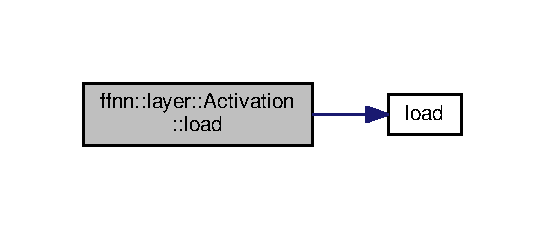
\includegraphics[width=262pt]{classffnn_1_1layer_1_1_activation_a045ecc330b67cdc3a41d6d7fc3a8dbf2_cgraph}
\end{center}
\end{figure}


\hypertarget{classffnn_1_1layer_1_1_activation_ab5525e49c08fc593856b9c95e0eba1ee}{\index{ffnn\-::layer\-::\-Activation@{ffnn\-::layer\-::\-Activation}!save@{save}}
\index{save@{save}!ffnn::layer::Activation@{ffnn\-::layer\-::\-Activation}}
\subsubsection[{save}]{\setlength{\rightskip}{0pt plus 5cm}template$<$typename Value\-Type, template$<$ class $>$ class Neuron\-Type, F\-F\-N\-N\-\_\-\-S\-I\-Z\-E\-\_\-\-T\-Y\-P\-E Size\-At\-Compile\-Time = Eigen\-::\-Dynamic$>$ void {\bf ffnn\-::layer\-::\-Activation}$<$ Value\-Type, Neuron\-Type, Size\-At\-Compile\-Time $>$\-::save (
\begin{DoxyParamCaption}
\item[{{\bf Output\-Archive} \&}]{ar, }
\item[{{\bf Version\-Type}}]{version}
\end{DoxyParamCaption}
) const\hspace{0.3cm}{\ttfamily [protected]}, {\ttfamily [virtual]}}}\label{classffnn_1_1layer_1_1_activation_ab5525e49c08fc593856b9c95e0eba1ee}


Save serializer. 



Reimplemented from \hyperlink{classffnn_1_1traits_1_1_unique_ad8be6fcb9a7519603b2aab19b3c6d593}{ffnn\-::traits\-::\-Unique}.



Here is the call graph for this function\-:\nopagebreak
\begin{figure}[H]
\begin{center}
\leavevmode
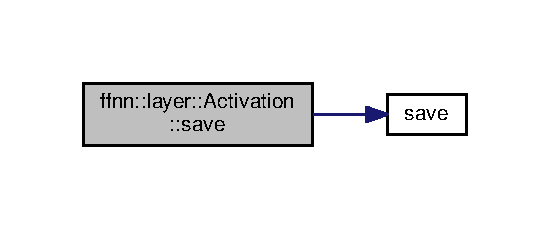
\includegraphics[width=264pt]{classffnn_1_1layer_1_1_activation_ab5525e49c08fc593856b9c95e0eba1ee_cgraph}
\end{center}
\end{figure}




The documentation for this class was generated from the following files\-:\begin{DoxyCompactItemize}
\item 
/home/briancairl/packages/src/ffnn-\/cpp/ffnn/include/ffnn/layer/\hyperlink{activation_8h}{activation.\-h}\item 
/home/briancairl/packages/src/ffnn-\/cpp/ffnn/include/ffnn/layer/impl/\hyperlink{activation_8hpp}{activation.\-hpp}\end{DoxyCompactItemize}

\hypertarget{classffnn_1_1optimizer_1_1_adam}{\section{ffnn\-:\-:optimizer\-:\-:Adam$<$ Layer\-Type $>$ Class Template Reference}
\label{classffnn_1_1optimizer_1_1_adam}\index{ffnn\-::optimizer\-::\-Adam$<$ Layer\-Type $>$@{ffnn\-::optimizer\-::\-Adam$<$ Layer\-Type $>$}}
}


{\ttfamily \#include \char`\"{}fwd.\-h\char`\"{}}



The documentation for this class was generated from the following file\-:\begin{DoxyCompactItemize}
\item 
/home/briancairl/packages/src/ffnn-\/cpp/ffnn/include/ffnn/optimizer/\hyperlink{fwd_8h}{fwd.\-h}\end{DoxyCompactItemize}

\hypertarget{classffnn_1_1optimizer_1_1_adam_3_01layer_1_1_fully_connected_3_01_value_type_00_01_inputs_at_co08ce471fd3ee7441a350cc42cfd35bcd}{\section{ffnn\-:\-:optimizer\-:\-:Adam$<$ layer\-:\-:Fully\-Connected$<$ Value\-Type, Inputs\-At\-Compile\-Time, Outputs\-At\-Compile\-Time $>$ $>$ Class Template Reference}
\label{classffnn_1_1optimizer_1_1_adam_3_01layer_1_1_fully_connected_3_01_value_type_00_01_inputs_at_co08ce471fd3ee7441a350cc42cfd35bcd}\index{ffnn\-::optimizer\-::\-Adam$<$ layer\-::\-Fully\-Connected$<$ Value\-Type, Inputs\-At\-Compile\-Time, Outputs\-At\-Compile\-Time $>$ $>$@{ffnn\-::optimizer\-::\-Adam$<$ layer\-::\-Fully\-Connected$<$ Value\-Type, Inputs\-At\-Compile\-Time, Outputs\-At\-Compile\-Time $>$ $>$}}
}


{\ttfamily \#include \char`\"{}fully\-\_\-connected.\-hpp\char`\"{}}



Inheritance diagram for ffnn\-:\-:optimizer\-:\-:Adam$<$ layer\-:\-:Fully\-Connected$<$ Value\-Type, Inputs\-At\-Compile\-Time, Outputs\-At\-Compile\-Time $>$ $>$\-:
\nopagebreak
\begin{figure}[H]
\begin{center}
\leavevmode
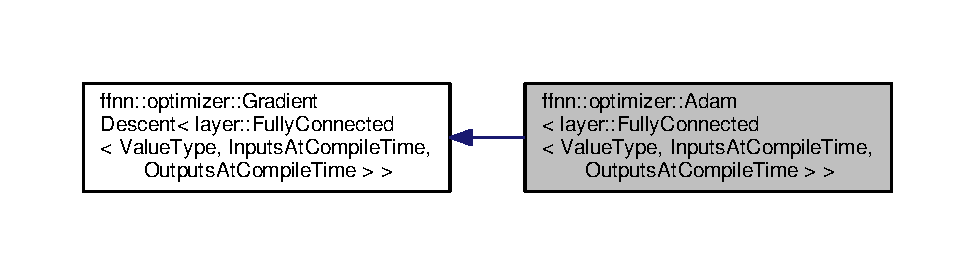
\includegraphics[width=350pt]{classffnn_1_1optimizer_1_1_adam_3_01layer_1_1_fully_connected_3_01_value_type_00_01_inputs_at_cobe2b9b06adffa70e04791567cce9f420}
\end{center}
\end{figure}


Collaboration diagram for ffnn\-:\-:optimizer\-:\-:Adam$<$ layer\-:\-:Fully\-Connected$<$ Value\-Type, Inputs\-At\-Compile\-Time, Outputs\-At\-Compile\-Time $>$ $>$\-:
\nopagebreak
\begin{figure}[H]
\begin{center}
\leavevmode
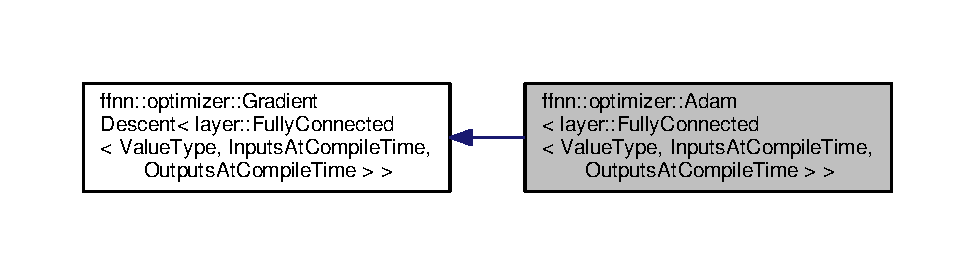
\includegraphics[width=350pt]{classffnn_1_1optimizer_1_1_adam_3_01layer_1_1_fully_connected_3_01_value_type_00_01_inputs_at_co5b19aea91ccd4a29fa3c61e22c78efee}
\end{center}
\end{figure}
\subsection*{Public Types}
\begin{DoxyCompactItemize}
\item 
typedef \hyperlink{classffnn_1_1layer_1_1_fully_connected}{layer\-::\-Fully\-Connected}\\*
$<$ Value\-Type, \\*
Inputs\-At\-Compile\-Time, \\*
Outputs\-At\-Compile\-Time $>$ \hyperlink{classffnn_1_1optimizer_1_1_adam_3_01layer_1_1_fully_connected_3_01_value_type_00_01_inputs_at_co08ce471fd3ee7441a350cc42cfd35bcd_ad82ece03afb695075874eaed356433d2}{Layer\-Type}
\begin{DoxyCompactList}\small\item\em Layer type standardization. \end{DoxyCompactList}\item 
typedef \hyperlink{classffnn_1_1optimizer_1_1_gradient_descent}{Gradient\-Descent}\\*
$<$ \hyperlink{classffnn_1_1optimizer_1_1_adam_3_01layer_1_1_fully_connected_3_01_value_type_00_01_inputs_at_co08ce471fd3ee7441a350cc42cfd35bcd_ad82ece03afb695075874eaed356433d2}{Layer\-Type} $>$ \hyperlink{classffnn_1_1optimizer_1_1_adam_3_01layer_1_1_fully_connected_3_01_value_type_00_01_inputs_at_co08ce471fd3ee7441a350cc42cfd35bcd_aa039b3368a2997e3437a32da6ef4a373}{Base}
\begin{DoxyCompactList}\small\item\em Base type standardization. \end{DoxyCompactList}\item 
typedef \hyperlink{classffnn_1_1layer_1_1_fully_connected_ac3ff6f72846f84f89c0d6e10f138c7e3}{Layer\-Type\-::\-Scalar\-Type} \hyperlink{classffnn_1_1optimizer_1_1_adam_3_01layer_1_1_fully_connected_3_01_value_type_00_01_inputs_at_co08ce471fd3ee7441a350cc42cfd35bcd_a3cd3f5a825a36308f81ff39f9dd51dd1}{Scalar\-Type}
\begin{DoxyCompactList}\small\item\em Scalar type standardization. \end{DoxyCompactList}\item 
typedef \hyperlink{classffnn_1_1layer_1_1_fully_connected_ae1b5e64828482a4c3eea0e2b0ba3f826}{Layer\-Type\-::\-Size\-Type} \hyperlink{classffnn_1_1optimizer_1_1_adam_3_01layer_1_1_fully_connected_3_01_value_type_00_01_inputs_at_co08ce471fd3ee7441a350cc42cfd35bcd_a6bbc6e181e5a5192b7b5cc42e3172372}{Size\-Type}
\begin{DoxyCompactList}\small\item\em Size type standardization. \end{DoxyCompactList}\item 
typedef \hyperlink{classffnn_1_1layer_1_1_fully_connected_a8fb8f9b598085d3a05214f38f70adfc7}{Layer\-Type\-::\-Input\-Block\-Type} \hyperlink{classffnn_1_1optimizer_1_1_adam_3_01layer_1_1_fully_connected_3_01_value_type_00_01_inputs_at_co08ce471fd3ee7441a350cc42cfd35bcd_a0f9a1a492d0763a6068fd01c3c8d705a}{Input\-Block\-Type}
\begin{DoxyCompactList}\small\item\em Matrix type standardization. \end{DoxyCompactList}\item 
typedef \hyperlink{classffnn_1_1layer_1_1_fully_connected_ac8c5ba1f20f470095c2c37f881f49814}{Layer\-Type\-::\-Output\-Block\-Type} \hyperlink{classffnn_1_1optimizer_1_1_adam_3_01layer_1_1_fully_connected_3_01_value_type_00_01_inputs_at_co08ce471fd3ee7441a350cc42cfd35bcd_a6b5ddc1adcb4bbc052bda25ac5ecef0b}{Output\-Block\-Type}
\begin{DoxyCompactList}\small\item\em Matrix type standardization. \end{DoxyCompactList}\item 
typedef \hyperlink{classffnn_1_1layer_1_1_fully_connected_a4ceb72064ac9a73a0907cc369d229da0}{Layer\-Type\-::\-Weight\-Matrix\-Type} \hyperlink{classffnn_1_1optimizer_1_1_adam_3_01layer_1_1_fully_connected_3_01_value_type_00_01_inputs_at_co08ce471fd3ee7441a350cc42cfd35bcd_aac2f4d3e444074ab554d2a0a45ba1daf}{Weight\-Matrix\-Type}
\begin{DoxyCompactList}\small\item\em Input-\/output weight matrix. \end{DoxyCompactList}\item 
typedef \hyperlink{classffnn_1_1layer_1_1_fully_connected_a926ff519682fa1bedd4c38159d5fd4bb}{Layer\-Type\-::\-Bias\-Vector\-Type} \hyperlink{classffnn_1_1optimizer_1_1_adam_3_01layer_1_1_fully_connected_3_01_value_type_00_01_inputs_at_co08ce471fd3ee7441a350cc42cfd35bcd_ac7a23bb92a19d1155a19feefbb5d366d}{Bias\-Vector\-Type}
\begin{DoxyCompactList}\small\item\em Bia vector type standardization. \end{DoxyCompactList}\end{DoxyCompactItemize}
\subsection*{Public Member Functions}
\begin{DoxyCompactItemize}
\item 
\hyperlink{classffnn_1_1optimizer_1_1_adam_3_01layer_1_1_fully_connected_3_01_value_type_00_01_inputs_at_co08ce471fd3ee7441a350cc42cfd35bcd_af3e2278852cdc5e2e3382992e36ccce3}{Adam} (\hyperlink{classffnn_1_1optimizer_1_1_adam_3_01layer_1_1_fully_connected_3_01_value_type_00_01_inputs_at_co08ce471fd3ee7441a350cc42cfd35bcd_a3cd3f5a825a36308f81ff39f9dd51dd1}{Scalar\-Type} lr, \hyperlink{classffnn_1_1optimizer_1_1_adam_3_01layer_1_1_fully_connected_3_01_value_type_00_01_inputs_at_co08ce471fd3ee7441a350cc42cfd35bcd_a3cd3f5a825a36308f81ff39f9dd51dd1}{Scalar\-Type} beta1=0.\-9, \hyperlink{classffnn_1_1optimizer_1_1_adam_3_01layer_1_1_fully_connected_3_01_value_type_00_01_inputs_at_co08ce471fd3ee7441a350cc42cfd35bcd_a3cd3f5a825a36308f81ff39f9dd51dd1}{Scalar\-Type} beta2=0.\-999, \hyperlink{classffnn_1_1optimizer_1_1_adam_3_01layer_1_1_fully_connected_3_01_value_type_00_01_inputs_at_co08ce471fd3ee7441a350cc42cfd35bcd_a3cd3f5a825a36308f81ff39f9dd51dd1}{Scalar\-Type} eps=1e-\/8)
\begin{DoxyCompactList}\small\item\em Setup constructor. \end{DoxyCompactList}\item 
virtual \hyperlink{classffnn_1_1optimizer_1_1_adam_3_01layer_1_1_fully_connected_3_01_value_type_00_01_inputs_at_co08ce471fd3ee7441a350cc42cfd35bcd_aa5cab60a5d10331e2e02ea932c58b2d0}{$\sim$\-Adam} ()
\item 
void \hyperlink{classffnn_1_1optimizer_1_1_adam_3_01layer_1_1_fully_connected_3_01_value_type_00_01_inputs_at_co08ce471fd3ee7441a350cc42cfd35bcd_aa67f949f7a1228c221d06b1b1e03c28b}{initialize} (\hyperlink{classffnn_1_1optimizer_1_1_adam_3_01layer_1_1_fully_connected_3_01_value_type_00_01_inputs_at_co08ce471fd3ee7441a350cc42cfd35bcd_ad82ece03afb695075874eaed356433d2}{Layer\-Type} \&layer)
\begin{DoxyCompactList}\small\item\em Initializes the \hyperlink{classffnn_1_1optimizer_1_1_optimizer}{Optimizer}. \end{DoxyCompactList}\item 
bool \hyperlink{classffnn_1_1optimizer_1_1_adam_3_01layer_1_1_fully_connected_3_01_value_type_00_01_inputs_at_co08ce471fd3ee7441a350cc42cfd35bcd_ad42586e39195fc9a72057f20b657f8be}{update} (\hyperlink{classffnn_1_1optimizer_1_1_adam_3_01layer_1_1_fully_connected_3_01_value_type_00_01_inputs_at_co08ce471fd3ee7441a350cc42cfd35bcd_ad82ece03afb695075874eaed356433d2}{Layer\-Type} \&layer)
\begin{DoxyCompactList}\small\item\em Applies optimization update. \end{DoxyCompactList}\end{DoxyCompactItemize}
\subsection*{Additional Inherited Members}


\subsection{Member Typedef Documentation}
\hypertarget{classffnn_1_1optimizer_1_1_adam_3_01layer_1_1_fully_connected_3_01_value_type_00_01_inputs_at_co08ce471fd3ee7441a350cc42cfd35bcd_aa039b3368a2997e3437a32da6ef4a373}{\index{ffnn\-::optimizer\-::\-Adam$<$ layer\-::\-Fully\-Connected$<$ Value\-Type, Inputs\-At\-Compile\-Time, Outputs\-At\-Compile\-Time $>$ $>$@{ffnn\-::optimizer\-::\-Adam$<$ layer\-::\-Fully\-Connected$<$ Value\-Type, Inputs\-At\-Compile\-Time, Outputs\-At\-Compile\-Time $>$ $>$}!Base@{Base}}
\index{Base@{Base}!ffnn::optimizer::Adam< layer::FullyConnected< ValueType, InputsAtCompileTime, OutputsAtCompileTime > >@{ffnn\-::optimizer\-::\-Adam$<$ layer\-::\-Fully\-Connected$<$ Value\-Type, Inputs\-At\-Compile\-Time, Outputs\-At\-Compile\-Time $>$ $>$}}
\subsubsection[{Base}]{\setlength{\rightskip}{0pt plus 5cm}typedef {\bf Gradient\-Descent}$<${\bf Layer\-Type}$>$ {\bf ffnn\-::optimizer\-::\-Adam}$<$ {\bf layer\-::\-Fully\-Connected}$<$ Value\-Type, Inputs\-At\-Compile\-Time, Outputs\-At\-Compile\-Time $>$ $>$\-::{\bf Base}}}\label{classffnn_1_1optimizer_1_1_adam_3_01layer_1_1_fully_connected_3_01_value_type_00_01_inputs_at_co08ce471fd3ee7441a350cc42cfd35bcd_aa039b3368a2997e3437a32da6ef4a373}


Base type standardization. 

\hypertarget{classffnn_1_1optimizer_1_1_adam_3_01layer_1_1_fully_connected_3_01_value_type_00_01_inputs_at_co08ce471fd3ee7441a350cc42cfd35bcd_ac7a23bb92a19d1155a19feefbb5d366d}{\index{ffnn\-::optimizer\-::\-Adam$<$ layer\-::\-Fully\-Connected$<$ Value\-Type, Inputs\-At\-Compile\-Time, Outputs\-At\-Compile\-Time $>$ $>$@{ffnn\-::optimizer\-::\-Adam$<$ layer\-::\-Fully\-Connected$<$ Value\-Type, Inputs\-At\-Compile\-Time, Outputs\-At\-Compile\-Time $>$ $>$}!Bias\-Vector\-Type@{Bias\-Vector\-Type}}
\index{Bias\-Vector\-Type@{Bias\-Vector\-Type}!ffnn::optimizer::Adam< layer::FullyConnected< ValueType, InputsAtCompileTime, OutputsAtCompileTime > >@{ffnn\-::optimizer\-::\-Adam$<$ layer\-::\-Fully\-Connected$<$ Value\-Type, Inputs\-At\-Compile\-Time, Outputs\-At\-Compile\-Time $>$ $>$}}
\subsubsection[{Bias\-Vector\-Type}]{\setlength{\rightskip}{0pt plus 5cm}typedef {\bf Layer\-Type\-::\-Bias\-Vector\-Type} {\bf ffnn\-::optimizer\-::\-Adam}$<$ {\bf layer\-::\-Fully\-Connected}$<$ Value\-Type, Inputs\-At\-Compile\-Time, Outputs\-At\-Compile\-Time $>$ $>$\-::{\bf Bias\-Vector\-Type}}}\label{classffnn_1_1optimizer_1_1_adam_3_01layer_1_1_fully_connected_3_01_value_type_00_01_inputs_at_co08ce471fd3ee7441a350cc42cfd35bcd_ac7a23bb92a19d1155a19feefbb5d366d}


Bia vector type standardization. 

\hypertarget{classffnn_1_1optimizer_1_1_adam_3_01layer_1_1_fully_connected_3_01_value_type_00_01_inputs_at_co08ce471fd3ee7441a350cc42cfd35bcd_a0f9a1a492d0763a6068fd01c3c8d705a}{\index{ffnn\-::optimizer\-::\-Adam$<$ layer\-::\-Fully\-Connected$<$ Value\-Type, Inputs\-At\-Compile\-Time, Outputs\-At\-Compile\-Time $>$ $>$@{ffnn\-::optimizer\-::\-Adam$<$ layer\-::\-Fully\-Connected$<$ Value\-Type, Inputs\-At\-Compile\-Time, Outputs\-At\-Compile\-Time $>$ $>$}!Input\-Block\-Type@{Input\-Block\-Type}}
\index{Input\-Block\-Type@{Input\-Block\-Type}!ffnn::optimizer::Adam< layer::FullyConnected< ValueType, InputsAtCompileTime, OutputsAtCompileTime > >@{ffnn\-::optimizer\-::\-Adam$<$ layer\-::\-Fully\-Connected$<$ Value\-Type, Inputs\-At\-Compile\-Time, Outputs\-At\-Compile\-Time $>$ $>$}}
\subsubsection[{Input\-Block\-Type}]{\setlength{\rightskip}{0pt plus 5cm}typedef {\bf Layer\-Type\-::\-Input\-Block\-Type} {\bf ffnn\-::optimizer\-::\-Adam}$<$ {\bf layer\-::\-Fully\-Connected}$<$ Value\-Type, Inputs\-At\-Compile\-Time, Outputs\-At\-Compile\-Time $>$ $>$\-::{\bf Input\-Block\-Type}}}\label{classffnn_1_1optimizer_1_1_adam_3_01layer_1_1_fully_connected_3_01_value_type_00_01_inputs_at_co08ce471fd3ee7441a350cc42cfd35bcd_a0f9a1a492d0763a6068fd01c3c8d705a}


Matrix type standardization. 

\hypertarget{classffnn_1_1optimizer_1_1_adam_3_01layer_1_1_fully_connected_3_01_value_type_00_01_inputs_at_co08ce471fd3ee7441a350cc42cfd35bcd_ad82ece03afb695075874eaed356433d2}{\index{ffnn\-::optimizer\-::\-Adam$<$ layer\-::\-Fully\-Connected$<$ Value\-Type, Inputs\-At\-Compile\-Time, Outputs\-At\-Compile\-Time $>$ $>$@{ffnn\-::optimizer\-::\-Adam$<$ layer\-::\-Fully\-Connected$<$ Value\-Type, Inputs\-At\-Compile\-Time, Outputs\-At\-Compile\-Time $>$ $>$}!Layer\-Type@{Layer\-Type}}
\index{Layer\-Type@{Layer\-Type}!ffnn::optimizer::Adam< layer::FullyConnected< ValueType, InputsAtCompileTime, OutputsAtCompileTime > >@{ffnn\-::optimizer\-::\-Adam$<$ layer\-::\-Fully\-Connected$<$ Value\-Type, Inputs\-At\-Compile\-Time, Outputs\-At\-Compile\-Time $>$ $>$}}
\subsubsection[{Layer\-Type}]{\setlength{\rightskip}{0pt plus 5cm}typedef {\bf layer\-::\-Fully\-Connected}$<$Value\-Type, Inputs\-At\-Compile\-Time, Outputs\-At\-Compile\-Time$>$ {\bf ffnn\-::optimizer\-::\-Adam}$<$ {\bf layer\-::\-Fully\-Connected}$<$ Value\-Type, Inputs\-At\-Compile\-Time, Outputs\-At\-Compile\-Time $>$ $>$\-::{\bf Layer\-Type}}}\label{classffnn_1_1optimizer_1_1_adam_3_01layer_1_1_fully_connected_3_01_value_type_00_01_inputs_at_co08ce471fd3ee7441a350cc42cfd35bcd_ad82ece03afb695075874eaed356433d2}


Layer type standardization. 

\hypertarget{classffnn_1_1optimizer_1_1_adam_3_01layer_1_1_fully_connected_3_01_value_type_00_01_inputs_at_co08ce471fd3ee7441a350cc42cfd35bcd_a6b5ddc1adcb4bbc052bda25ac5ecef0b}{\index{ffnn\-::optimizer\-::\-Adam$<$ layer\-::\-Fully\-Connected$<$ Value\-Type, Inputs\-At\-Compile\-Time, Outputs\-At\-Compile\-Time $>$ $>$@{ffnn\-::optimizer\-::\-Adam$<$ layer\-::\-Fully\-Connected$<$ Value\-Type, Inputs\-At\-Compile\-Time, Outputs\-At\-Compile\-Time $>$ $>$}!Output\-Block\-Type@{Output\-Block\-Type}}
\index{Output\-Block\-Type@{Output\-Block\-Type}!ffnn::optimizer::Adam< layer::FullyConnected< ValueType, InputsAtCompileTime, OutputsAtCompileTime > >@{ffnn\-::optimizer\-::\-Adam$<$ layer\-::\-Fully\-Connected$<$ Value\-Type, Inputs\-At\-Compile\-Time, Outputs\-At\-Compile\-Time $>$ $>$}}
\subsubsection[{Output\-Block\-Type}]{\setlength{\rightskip}{0pt plus 5cm}typedef {\bf Layer\-Type\-::\-Output\-Block\-Type} {\bf ffnn\-::optimizer\-::\-Adam}$<$ {\bf layer\-::\-Fully\-Connected}$<$ Value\-Type, Inputs\-At\-Compile\-Time, Outputs\-At\-Compile\-Time $>$ $>$\-::{\bf Output\-Block\-Type}}}\label{classffnn_1_1optimizer_1_1_adam_3_01layer_1_1_fully_connected_3_01_value_type_00_01_inputs_at_co08ce471fd3ee7441a350cc42cfd35bcd_a6b5ddc1adcb4bbc052bda25ac5ecef0b}


Matrix type standardization. 

\hypertarget{classffnn_1_1optimizer_1_1_adam_3_01layer_1_1_fully_connected_3_01_value_type_00_01_inputs_at_co08ce471fd3ee7441a350cc42cfd35bcd_a3cd3f5a825a36308f81ff39f9dd51dd1}{\index{ffnn\-::optimizer\-::\-Adam$<$ layer\-::\-Fully\-Connected$<$ Value\-Type, Inputs\-At\-Compile\-Time, Outputs\-At\-Compile\-Time $>$ $>$@{ffnn\-::optimizer\-::\-Adam$<$ layer\-::\-Fully\-Connected$<$ Value\-Type, Inputs\-At\-Compile\-Time, Outputs\-At\-Compile\-Time $>$ $>$}!Scalar\-Type@{Scalar\-Type}}
\index{Scalar\-Type@{Scalar\-Type}!ffnn::optimizer::Adam< layer::FullyConnected< ValueType, InputsAtCompileTime, OutputsAtCompileTime > >@{ffnn\-::optimizer\-::\-Adam$<$ layer\-::\-Fully\-Connected$<$ Value\-Type, Inputs\-At\-Compile\-Time, Outputs\-At\-Compile\-Time $>$ $>$}}
\subsubsection[{Scalar\-Type}]{\setlength{\rightskip}{0pt plus 5cm}typedef {\bf Layer\-Type\-::\-Scalar\-Type} {\bf ffnn\-::optimizer\-::\-Adam}$<$ {\bf layer\-::\-Fully\-Connected}$<$ Value\-Type, Inputs\-At\-Compile\-Time, Outputs\-At\-Compile\-Time $>$ $>$\-::{\bf Scalar\-Type}}}\label{classffnn_1_1optimizer_1_1_adam_3_01layer_1_1_fully_connected_3_01_value_type_00_01_inputs_at_co08ce471fd3ee7441a350cc42cfd35bcd_a3cd3f5a825a36308f81ff39f9dd51dd1}


Scalar type standardization. 

\hypertarget{classffnn_1_1optimizer_1_1_adam_3_01layer_1_1_fully_connected_3_01_value_type_00_01_inputs_at_co08ce471fd3ee7441a350cc42cfd35bcd_a6bbc6e181e5a5192b7b5cc42e3172372}{\index{ffnn\-::optimizer\-::\-Adam$<$ layer\-::\-Fully\-Connected$<$ Value\-Type, Inputs\-At\-Compile\-Time, Outputs\-At\-Compile\-Time $>$ $>$@{ffnn\-::optimizer\-::\-Adam$<$ layer\-::\-Fully\-Connected$<$ Value\-Type, Inputs\-At\-Compile\-Time, Outputs\-At\-Compile\-Time $>$ $>$}!Size\-Type@{Size\-Type}}
\index{Size\-Type@{Size\-Type}!ffnn::optimizer::Adam< layer::FullyConnected< ValueType, InputsAtCompileTime, OutputsAtCompileTime > >@{ffnn\-::optimizer\-::\-Adam$<$ layer\-::\-Fully\-Connected$<$ Value\-Type, Inputs\-At\-Compile\-Time, Outputs\-At\-Compile\-Time $>$ $>$}}
\subsubsection[{Size\-Type}]{\setlength{\rightskip}{0pt plus 5cm}typedef {\bf Layer\-Type\-::\-Size\-Type} {\bf ffnn\-::optimizer\-::\-Adam}$<$ {\bf layer\-::\-Fully\-Connected}$<$ Value\-Type, Inputs\-At\-Compile\-Time, Outputs\-At\-Compile\-Time $>$ $>$\-::{\bf Size\-Type}}}\label{classffnn_1_1optimizer_1_1_adam_3_01layer_1_1_fully_connected_3_01_value_type_00_01_inputs_at_co08ce471fd3ee7441a350cc42cfd35bcd_a6bbc6e181e5a5192b7b5cc42e3172372}


Size type standardization. 

\hypertarget{classffnn_1_1optimizer_1_1_adam_3_01layer_1_1_fully_connected_3_01_value_type_00_01_inputs_at_co08ce471fd3ee7441a350cc42cfd35bcd_aac2f4d3e444074ab554d2a0a45ba1daf}{\index{ffnn\-::optimizer\-::\-Adam$<$ layer\-::\-Fully\-Connected$<$ Value\-Type, Inputs\-At\-Compile\-Time, Outputs\-At\-Compile\-Time $>$ $>$@{ffnn\-::optimizer\-::\-Adam$<$ layer\-::\-Fully\-Connected$<$ Value\-Type, Inputs\-At\-Compile\-Time, Outputs\-At\-Compile\-Time $>$ $>$}!Weight\-Matrix\-Type@{Weight\-Matrix\-Type}}
\index{Weight\-Matrix\-Type@{Weight\-Matrix\-Type}!ffnn::optimizer::Adam< layer::FullyConnected< ValueType, InputsAtCompileTime, OutputsAtCompileTime > >@{ffnn\-::optimizer\-::\-Adam$<$ layer\-::\-Fully\-Connected$<$ Value\-Type, Inputs\-At\-Compile\-Time, Outputs\-At\-Compile\-Time $>$ $>$}}
\subsubsection[{Weight\-Matrix\-Type}]{\setlength{\rightskip}{0pt plus 5cm}typedef {\bf Layer\-Type\-::\-Weight\-Matrix\-Type} {\bf ffnn\-::optimizer\-::\-Adam}$<$ {\bf layer\-::\-Fully\-Connected}$<$ Value\-Type, Inputs\-At\-Compile\-Time, Outputs\-At\-Compile\-Time $>$ $>$\-::{\bf Weight\-Matrix\-Type}}}\label{classffnn_1_1optimizer_1_1_adam_3_01layer_1_1_fully_connected_3_01_value_type_00_01_inputs_at_co08ce471fd3ee7441a350cc42cfd35bcd_aac2f4d3e444074ab554d2a0a45ba1daf}


Input-\/output weight matrix. 



\subsection{Constructor \& Destructor Documentation}
\hypertarget{classffnn_1_1optimizer_1_1_adam_3_01layer_1_1_fully_connected_3_01_value_type_00_01_inputs_at_co08ce471fd3ee7441a350cc42cfd35bcd_af3e2278852cdc5e2e3382992e36ccce3}{\index{ffnn\-::optimizer\-::\-Adam$<$ layer\-::\-Fully\-Connected$<$ Value\-Type, Inputs\-At\-Compile\-Time, Outputs\-At\-Compile\-Time $>$ $>$@{ffnn\-::optimizer\-::\-Adam$<$ layer\-::\-Fully\-Connected$<$ Value\-Type, Inputs\-At\-Compile\-Time, Outputs\-At\-Compile\-Time $>$ $>$}!Adam@{Adam}}
\index{Adam@{Adam}!ffnn::optimizer::Adam< layer::FullyConnected< ValueType, InputsAtCompileTime, OutputsAtCompileTime > >@{ffnn\-::optimizer\-::\-Adam$<$ layer\-::\-Fully\-Connected$<$ Value\-Type, Inputs\-At\-Compile\-Time, Outputs\-At\-Compile\-Time $>$ $>$}}
\subsubsection[{Adam}]{\setlength{\rightskip}{0pt plus 5cm}{\bf ffnn\-::optimizer\-::\-Adam}$<$ {\bf layer\-::\-Fully\-Connected}$<$ Value\-Type, Inputs\-At\-Compile\-Time, Outputs\-At\-Compile\-Time $>$ $>$\-::{\bf Adam} (
\begin{DoxyParamCaption}
\item[{{\bf Scalar\-Type}}]{lr, }
\item[{{\bf Scalar\-Type}}]{beta1 = {\ttfamily 0.9}, }
\item[{{\bf Scalar\-Type}}]{beta2 = {\ttfamily 0.999}, }
\item[{{\bf Scalar\-Type}}]{eps = {\ttfamily 1e-\/8}}
\end{DoxyParamCaption}
)\hspace{0.3cm}{\ttfamily [inline]}, {\ttfamily [explicit]}}}\label{classffnn_1_1optimizer_1_1_adam_3_01layer_1_1_fully_connected_3_01_value_type_00_01_inputs_at_co08ce471fd3ee7441a350cc42cfd35bcd_af3e2278852cdc5e2e3382992e36ccce3}


Setup constructor. 


\begin{DoxyParams}{Parameters}
{\em lr} & Learning rate \\
\hline
\end{DoxyParams}
\hypertarget{classffnn_1_1optimizer_1_1_adam_3_01layer_1_1_fully_connected_3_01_value_type_00_01_inputs_at_co08ce471fd3ee7441a350cc42cfd35bcd_aa5cab60a5d10331e2e02ea932c58b2d0}{\index{ffnn\-::optimizer\-::\-Adam$<$ layer\-::\-Fully\-Connected$<$ Value\-Type, Inputs\-At\-Compile\-Time, Outputs\-At\-Compile\-Time $>$ $>$@{ffnn\-::optimizer\-::\-Adam$<$ layer\-::\-Fully\-Connected$<$ Value\-Type, Inputs\-At\-Compile\-Time, Outputs\-At\-Compile\-Time $>$ $>$}!$\sim$\-Adam@{$\sim$\-Adam}}
\index{$\sim$\-Adam@{$\sim$\-Adam}!ffnn::optimizer::Adam< layer::FullyConnected< ValueType, InputsAtCompileTime, OutputsAtCompileTime > >@{ffnn\-::optimizer\-::\-Adam$<$ layer\-::\-Fully\-Connected$<$ Value\-Type, Inputs\-At\-Compile\-Time, Outputs\-At\-Compile\-Time $>$ $>$}}
\subsubsection[{$\sim$\-Adam}]{\setlength{\rightskip}{0pt plus 5cm}virtual {\bf ffnn\-::optimizer\-::\-Adam}$<$ {\bf layer\-::\-Fully\-Connected}$<$ Value\-Type, Inputs\-At\-Compile\-Time, Outputs\-At\-Compile\-Time $>$ $>$\-::$\sim${\bf Adam} (
\begin{DoxyParamCaption}
{}
\end{DoxyParamCaption}
)\hspace{0.3cm}{\ttfamily [inline]}, {\ttfamily [virtual]}}}\label{classffnn_1_1optimizer_1_1_adam_3_01layer_1_1_fully_connected_3_01_value_type_00_01_inputs_at_co08ce471fd3ee7441a350cc42cfd35bcd_aa5cab60a5d10331e2e02ea932c58b2d0}


\subsection{Member Function Documentation}
\hypertarget{classffnn_1_1optimizer_1_1_adam_3_01layer_1_1_fully_connected_3_01_value_type_00_01_inputs_at_co08ce471fd3ee7441a350cc42cfd35bcd_aa67f949f7a1228c221d06b1b1e03c28b}{\index{ffnn\-::optimizer\-::\-Adam$<$ layer\-::\-Fully\-Connected$<$ Value\-Type, Inputs\-At\-Compile\-Time, Outputs\-At\-Compile\-Time $>$ $>$@{ffnn\-::optimizer\-::\-Adam$<$ layer\-::\-Fully\-Connected$<$ Value\-Type, Inputs\-At\-Compile\-Time, Outputs\-At\-Compile\-Time $>$ $>$}!initialize@{initialize}}
\index{initialize@{initialize}!ffnn::optimizer::Adam< layer::FullyConnected< ValueType, InputsAtCompileTime, OutputsAtCompileTime > >@{ffnn\-::optimizer\-::\-Adam$<$ layer\-::\-Fully\-Connected$<$ Value\-Type, Inputs\-At\-Compile\-Time, Outputs\-At\-Compile\-Time $>$ $>$}}
\subsubsection[{initialize}]{\setlength{\rightskip}{0pt plus 5cm}void {\bf ffnn\-::optimizer\-::\-Adam}$<$ {\bf layer\-::\-Fully\-Connected}$<$ Value\-Type, Inputs\-At\-Compile\-Time, Outputs\-At\-Compile\-Time $>$ $>$\-::initialize (
\begin{DoxyParamCaption}
\item[{{\bf Layer\-Type} \&}]{layer}
\end{DoxyParamCaption}
)\hspace{0.3cm}{\ttfamily [inline]}, {\ttfamily [virtual]}}}\label{classffnn_1_1optimizer_1_1_adam_3_01layer_1_1_fully_connected_3_01_value_type_00_01_inputs_at_co08ce471fd3ee7441a350cc42cfd35bcd_aa67f949f7a1228c221d06b1b1e03c28b}


Initializes the \hyperlink{classffnn_1_1optimizer_1_1_optimizer}{Optimizer}. 


\begin{DoxyParams}[1]{Parameters}
\mbox{\tt in,out}  & {\em layer} & Layer to optimize \\
\hline
\end{DoxyParams}


Reimplemented from \hyperlink{classffnn_1_1optimizer_1_1_gradient_descent_3_01layer_1_1_fully_connected_3_01_value_type_00_01_5f7b01db2ae4d39760d70ee323649a60_a2e152e94571b7948b514c9d4cbd70504}{ffnn\-::optimizer\-::\-Gradient\-Descent$<$ layer\-::\-Fully\-Connected$<$ Value\-Type, Inputs\-At\-Compile\-Time, Outputs\-At\-Compile\-Time $>$ $>$}.



Here is the call graph for this function\-:
\nopagebreak
\begin{figure}[H]
\begin{center}
\leavevmode
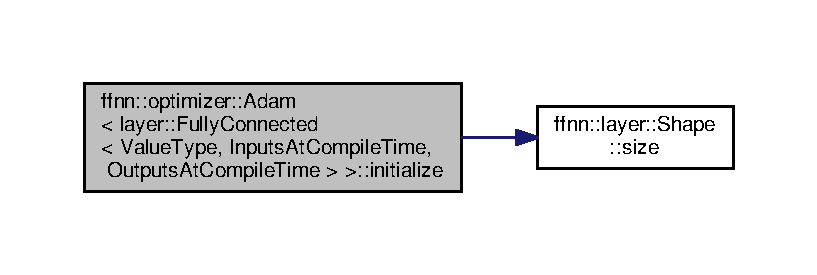
\includegraphics[width=350pt]{classffnn_1_1optimizer_1_1_adam_3_01layer_1_1_fully_connected_3_01_value_type_00_01_inputs_at_co08ce471fd3ee7441a350cc42cfd35bcd_aa67f949f7a1228c221d06b1b1e03c28b_cgraph}
\end{center}
\end{figure}


\hypertarget{classffnn_1_1optimizer_1_1_adam_3_01layer_1_1_fully_connected_3_01_value_type_00_01_inputs_at_co08ce471fd3ee7441a350cc42cfd35bcd_ad42586e39195fc9a72057f20b657f8be}{\index{ffnn\-::optimizer\-::\-Adam$<$ layer\-::\-Fully\-Connected$<$ Value\-Type, Inputs\-At\-Compile\-Time, Outputs\-At\-Compile\-Time $>$ $>$@{ffnn\-::optimizer\-::\-Adam$<$ layer\-::\-Fully\-Connected$<$ Value\-Type, Inputs\-At\-Compile\-Time, Outputs\-At\-Compile\-Time $>$ $>$}!update@{update}}
\index{update@{update}!ffnn::optimizer::Adam< layer::FullyConnected< ValueType, InputsAtCompileTime, OutputsAtCompileTime > >@{ffnn\-::optimizer\-::\-Adam$<$ layer\-::\-Fully\-Connected$<$ Value\-Type, Inputs\-At\-Compile\-Time, Outputs\-At\-Compile\-Time $>$ $>$}}
\subsubsection[{update}]{\setlength{\rightskip}{0pt plus 5cm}bool {\bf ffnn\-::optimizer\-::\-Adam}$<$ {\bf layer\-::\-Fully\-Connected}$<$ Value\-Type, Inputs\-At\-Compile\-Time, Outputs\-At\-Compile\-Time $>$ $>$\-::update (
\begin{DoxyParamCaption}
\item[{{\bf Layer\-Type} \&}]{layer}
\end{DoxyParamCaption}
)\hspace{0.3cm}{\ttfamily [inline]}, {\ttfamily [virtual]}}}\label{classffnn_1_1optimizer_1_1_adam_3_01layer_1_1_fully_connected_3_01_value_type_00_01_inputs_at_co08ce471fd3ee7441a350cc42cfd35bcd_ad42586e39195fc9a72057f20b657f8be}


Applies optimization update. 


\begin{DoxyParams}[1]{Parameters}
\mbox{\tt in,out}  & {\em layer} & Layer to optimize \\
\hline
\end{DoxyParams}

\begin{DoxyRetVals}{Return values}
{\em true} & if optimization update was applied successfully \\
\hline
{\em false} & otherwise \\
\hline
\end{DoxyRetVals}


Reimplemented from \hyperlink{classffnn_1_1optimizer_1_1_gradient_descent_3_01layer_1_1_fully_connected_3_01_value_type_00_01_5f7b01db2ae4d39760d70ee323649a60_a4e15c26f4b561a8ea3ca3de3b324e1cf}{ffnn\-::optimizer\-::\-Gradient\-Descent$<$ layer\-::\-Fully\-Connected$<$ Value\-Type, Inputs\-At\-Compile\-Time, Outputs\-At\-Compile\-Time $>$ $>$}.



Here is the call graph for this function\-:
\nopagebreak
\begin{figure}[H]
\begin{center}
\leavevmode
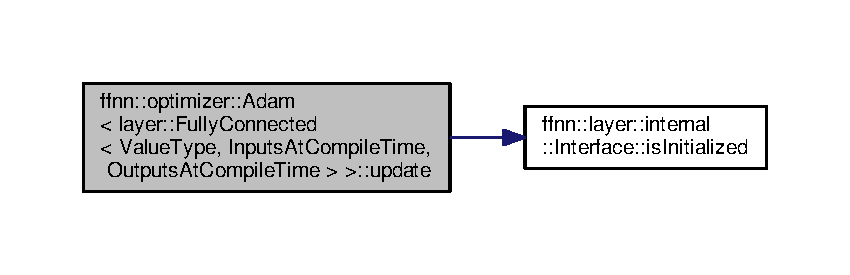
\includegraphics[width=350pt]{classffnn_1_1optimizer_1_1_adam_3_01layer_1_1_fully_connected_3_01_value_type_00_01_inputs_at_co08ce471fd3ee7441a350cc42cfd35bcd_ad42586e39195fc9a72057f20b657f8be_cgraph}
\end{center}
\end{figure}




The documentation for this class was generated from the following file\-:\begin{DoxyCompactItemize}
\item 
/home/briancairl/packages/src/ffnn-\/cpp/ffnn/include/ffnn/optimizer/impl/adam/\hyperlink{optimizer_2impl_2adam_2fully__connected_8hpp}{fully\-\_\-connected.\-hpp}\end{DoxyCompactItemize}

\hypertarget{classffnn_1_1optimizer_1_1_adam_3_01layer_1_1_sparsely_connected_3_01_value_type_00_01_inputs_at5101e46d32858ec2169acdeede08d723}{\section{ffnn\-:\-:optimizer\-:\-:Adam$<$ layer\-:\-:Sparsely\-Connected$<$ Value\-Type, Inputs\-At\-Compile\-Time, Outputs\-At\-Compile\-Time $>$ $>$ Class Template Reference}
\label{classffnn_1_1optimizer_1_1_adam_3_01layer_1_1_sparsely_connected_3_01_value_type_00_01_inputs_at5101e46d32858ec2169acdeede08d723}\index{ffnn\-::optimizer\-::\-Adam$<$ layer\-::\-Sparsely\-Connected$<$ Value\-Type, Inputs\-At\-Compile\-Time, Outputs\-At\-Compile\-Time $>$ $>$@{ffnn\-::optimizer\-::\-Adam$<$ layer\-::\-Sparsely\-Connected$<$ Value\-Type, Inputs\-At\-Compile\-Time, Outputs\-At\-Compile\-Time $>$ $>$}}
}


{\ttfamily \#include \char`\"{}sparsely\-\_\-connected.\-hpp\char`\"{}}



Inheritance diagram for ffnn\-:\-:optimizer\-:\-:Adam$<$ layer\-:\-:Sparsely\-Connected$<$ Value\-Type, Inputs\-At\-Compile\-Time, Outputs\-At\-Compile\-Time $>$ $>$\-:
\nopagebreak
\begin{figure}[H]
\begin{center}
\leavevmode
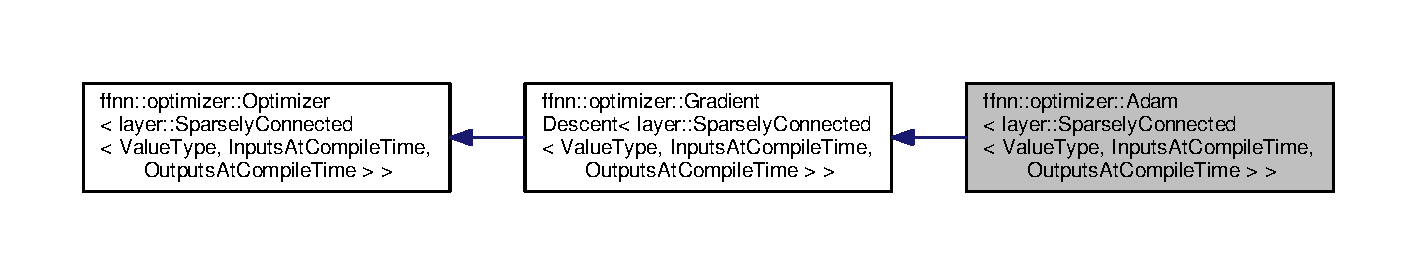
\includegraphics[width=350pt]{classffnn_1_1optimizer_1_1_adam_3_01layer_1_1_sparsely_connected_3_01_value_type_00_01_inputs_atceca5391622640783f2a5e090f69ef26}
\end{center}
\end{figure}


Collaboration diagram for ffnn\-:\-:optimizer\-:\-:Adam$<$ layer\-:\-:Sparsely\-Connected$<$ Value\-Type, Inputs\-At\-Compile\-Time, Outputs\-At\-Compile\-Time $>$ $>$\-:
\nopagebreak
\begin{figure}[H]
\begin{center}
\leavevmode
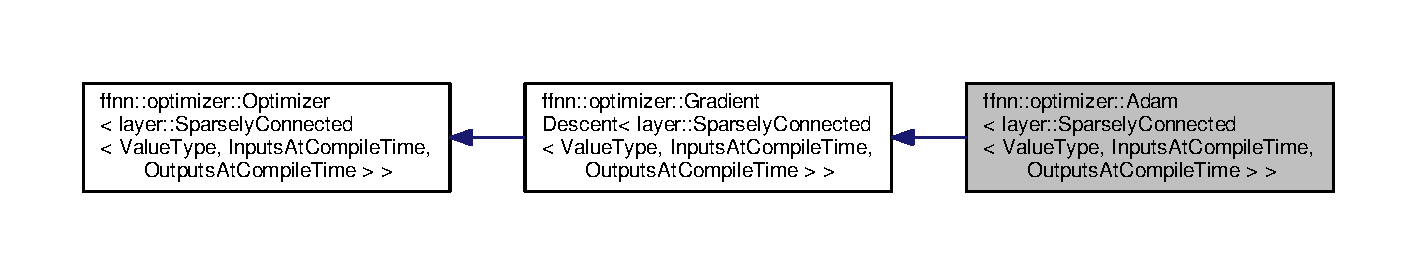
\includegraphics[width=350pt]{classffnn_1_1optimizer_1_1_adam_3_01layer_1_1_sparsely_connected_3_01_value_type_00_01_inputs_atb682edad999429458f7de6145c1fc052}
\end{center}
\end{figure}
\subsection*{Public Types}
\begin{DoxyCompactItemize}
\item 
typedef \\*
\hyperlink{classffnn_1_1layer_1_1_sparsely_connected}{layer\-::\-Sparsely\-Connected}\\*
$<$ Value\-Type, \\*
Inputs\-At\-Compile\-Time, \\*
Outputs\-At\-Compile\-Time $>$ \hyperlink{classffnn_1_1optimizer_1_1_adam_3_01layer_1_1_sparsely_connected_3_01_value_type_00_01_inputs_at5101e46d32858ec2169acdeede08d723_af2f04c26de6845836cd595df5caaeaf9}{Layer\-Type}
\begin{DoxyCompactList}\small\item\em Layer type standardization. \end{DoxyCompactList}\item 
typedef \hyperlink{classffnn_1_1optimizer_1_1_gradient_descent}{Gradient\-Descent}\\*
$<$ \hyperlink{classffnn_1_1optimizer_1_1_adam_3_01layer_1_1_sparsely_connected_3_01_value_type_00_01_inputs_at5101e46d32858ec2169acdeede08d723_af2f04c26de6845836cd595df5caaeaf9}{Layer\-Type} $>$ \hyperlink{classffnn_1_1optimizer_1_1_adam_3_01layer_1_1_sparsely_connected_3_01_value_type_00_01_inputs_at5101e46d32858ec2169acdeede08d723_aa291802e48ddc12f1d15293989679f43}{Base}
\begin{DoxyCompactList}\small\item\em Base type standardization. \end{DoxyCompactList}\item 
typedef \hyperlink{classffnn_1_1layer_1_1_sparsely_connected_abe2b75254f39c0bec9f02b2e906e7919}{Layer\-Type\-::\-Scalar\-Type} \hyperlink{classffnn_1_1optimizer_1_1_adam_3_01layer_1_1_sparsely_connected_3_01_value_type_00_01_inputs_at5101e46d32858ec2169acdeede08d723_acbcaaadfd5e5ad46a775e89024f96ec5}{Scalar\-Type}
\begin{DoxyCompactList}\small\item\em Scalar type standardization. \end{DoxyCompactList}\item 
typedef \hyperlink{classffnn_1_1layer_1_1_sparsely_connected_a86b75c2723c1f8b6771224257f5eb1c1}{Layer\-Type\-::\-Size\-Type} \hyperlink{classffnn_1_1optimizer_1_1_adam_3_01layer_1_1_sparsely_connected_3_01_value_type_00_01_inputs_at5101e46d32858ec2169acdeede08d723_a4801eb026ada106bb4134b312e557395}{Size\-Type}
\begin{DoxyCompactList}\small\item\em Size type standardization. \end{DoxyCompactList}\item 
typedef \hyperlink{classffnn_1_1layer_1_1_sparsely_connected_ad90fd9b4c687e4dc515cf8ca2796043c}{Layer\-Type\-::\-Input\-Block\-Type} \hyperlink{classffnn_1_1optimizer_1_1_adam_3_01layer_1_1_sparsely_connected_3_01_value_type_00_01_inputs_at5101e46d32858ec2169acdeede08d723_a91ec5d1a25381d6c8e864474bd5e5817}{Input\-Block\-Type}
\begin{DoxyCompactList}\small\item\em Matrix type standardization. \end{DoxyCompactList}\item 
typedef \hyperlink{classffnn_1_1layer_1_1_sparsely_connected_aacf4fb49a3f57aba90e55d8d3c63cf45}{Layer\-Type\-::\-Output\-Block\-Type} \hyperlink{classffnn_1_1optimizer_1_1_adam_3_01layer_1_1_sparsely_connected_3_01_value_type_00_01_inputs_at5101e46d32858ec2169acdeede08d723_ae206d0e2b950f865445e348697b9d6ab}{Output\-Block\-Type}
\begin{DoxyCompactList}\small\item\em Matrix type standardization. \end{DoxyCompactList}\item 
typedef \hyperlink{classffnn_1_1layer_1_1_sparsely_connected_acafafa368b81042965eed9607cad2dbd}{Layer\-Type\-::\-Weight\-Matrix\-Type} \hyperlink{classffnn_1_1optimizer_1_1_adam_3_01layer_1_1_sparsely_connected_3_01_value_type_00_01_inputs_at5101e46d32858ec2169acdeede08d723_a72391596a110863096101fc02984db1e}{Weight\-Matrix\-Type}
\begin{DoxyCompactList}\small\item\em Input-\/output weight matrix. \end{DoxyCompactList}\item 
typedef \hyperlink{classffnn_1_1layer_1_1_sparsely_connected_ad2d566cbb6c54c8723d79737075b4a00}{Layer\-Type\-::\-Bias\-Vector\-Type} \hyperlink{classffnn_1_1optimizer_1_1_adam_3_01layer_1_1_sparsely_connected_3_01_value_type_00_01_inputs_at5101e46d32858ec2169acdeede08d723_aa4156bd11aaf893cfed8f3390f29c182}{Bias\-Vector\-Type}
\begin{DoxyCompactList}\small\item\em Bia vector type standardization. \end{DoxyCompactList}\end{DoxyCompactItemize}
\subsection*{Public Member Functions}
\begin{DoxyCompactItemize}
\item 
\hyperlink{classffnn_1_1optimizer_1_1_adam_3_01layer_1_1_sparsely_connected_3_01_value_type_00_01_inputs_at5101e46d32858ec2169acdeede08d723_a58cbea05b475e4cf96e1ed481e5755ef}{Adam} (\hyperlink{classffnn_1_1optimizer_1_1_adam_3_01layer_1_1_sparsely_connected_3_01_value_type_00_01_inputs_at5101e46d32858ec2169acdeede08d723_acbcaaadfd5e5ad46a775e89024f96ec5}{Scalar\-Type} lr, \hyperlink{classffnn_1_1optimizer_1_1_adam_3_01layer_1_1_sparsely_connected_3_01_value_type_00_01_inputs_at5101e46d32858ec2169acdeede08d723_acbcaaadfd5e5ad46a775e89024f96ec5}{Scalar\-Type} beta1=0.\-9, \hyperlink{classffnn_1_1optimizer_1_1_adam_3_01layer_1_1_sparsely_connected_3_01_value_type_00_01_inputs_at5101e46d32858ec2169acdeede08d723_acbcaaadfd5e5ad46a775e89024f96ec5}{Scalar\-Type} beta2=0.\-999, \hyperlink{classffnn_1_1optimizer_1_1_adam_3_01layer_1_1_sparsely_connected_3_01_value_type_00_01_inputs_at5101e46d32858ec2169acdeede08d723_acbcaaadfd5e5ad46a775e89024f96ec5}{Scalar\-Type} eps=1e-\/8)
\begin{DoxyCompactList}\small\item\em Setup constructor. \end{DoxyCompactList}\item 
virtual \hyperlink{classffnn_1_1optimizer_1_1_adam_3_01layer_1_1_sparsely_connected_3_01_value_type_00_01_inputs_at5101e46d32858ec2169acdeede08d723_a131e9e3dfb840c43f20c661681e92dc1}{$\sim$\-Adam} ()
\item 
void \hyperlink{classffnn_1_1optimizer_1_1_adam_3_01layer_1_1_sparsely_connected_3_01_value_type_00_01_inputs_at5101e46d32858ec2169acdeede08d723_a3529c6f6fb1befc882cc3ae17c00ba5a}{initialize} (\hyperlink{classffnn_1_1optimizer_1_1_adam_3_01layer_1_1_sparsely_connected_3_01_value_type_00_01_inputs_at5101e46d32858ec2169acdeede08d723_af2f04c26de6845836cd595df5caaeaf9}{Layer\-Type} \&layer)
\begin{DoxyCompactList}\small\item\em Initializes the \hyperlink{classffnn_1_1optimizer_1_1_optimizer}{Optimizer}. \end{DoxyCompactList}\item 
bool \hyperlink{classffnn_1_1optimizer_1_1_adam_3_01layer_1_1_sparsely_connected_3_01_value_type_00_01_inputs_at5101e46d32858ec2169acdeede08d723_aaa3b2eb55a9d80d51330c132df65214b}{update} (\hyperlink{classffnn_1_1optimizer_1_1_adam_3_01layer_1_1_sparsely_connected_3_01_value_type_00_01_inputs_at5101e46d32858ec2169acdeede08d723_af2f04c26de6845836cd595df5caaeaf9}{Layer\-Type} \&layer)
\begin{DoxyCompactList}\small\item\em Applies optimization update. \end{DoxyCompactList}\end{DoxyCompactItemize}
\subsection*{Additional Inherited Members}


\subsection{Member Typedef Documentation}
\hypertarget{classffnn_1_1optimizer_1_1_adam_3_01layer_1_1_sparsely_connected_3_01_value_type_00_01_inputs_at5101e46d32858ec2169acdeede08d723_aa291802e48ddc12f1d15293989679f43}{\index{ffnn\-::optimizer\-::\-Adam$<$ layer\-::\-Sparsely\-Connected$<$ Value\-Type, Inputs\-At\-Compile\-Time, Outputs\-At\-Compile\-Time $>$ $>$@{ffnn\-::optimizer\-::\-Adam$<$ layer\-::\-Sparsely\-Connected$<$ Value\-Type, Inputs\-At\-Compile\-Time, Outputs\-At\-Compile\-Time $>$ $>$}!Base@{Base}}
\index{Base@{Base}!ffnn::optimizer::Adam< layer::SparselyConnected< ValueType, InputsAtCompileTime, OutputsAtCompileTime > >@{ffnn\-::optimizer\-::\-Adam$<$ layer\-::\-Sparsely\-Connected$<$ Value\-Type, Inputs\-At\-Compile\-Time, Outputs\-At\-Compile\-Time $>$ $>$}}
\subsubsection[{Base}]{\setlength{\rightskip}{0pt plus 5cm}typedef {\bf Gradient\-Descent}$<${\bf Layer\-Type}$>$ {\bf ffnn\-::optimizer\-::\-Adam}$<$ {\bf layer\-::\-Sparsely\-Connected}$<$ Value\-Type, Inputs\-At\-Compile\-Time, Outputs\-At\-Compile\-Time $>$ $>$\-::{\bf Base}}}\label{classffnn_1_1optimizer_1_1_adam_3_01layer_1_1_sparsely_connected_3_01_value_type_00_01_inputs_at5101e46d32858ec2169acdeede08d723_aa291802e48ddc12f1d15293989679f43}


Base type standardization. 

\hypertarget{classffnn_1_1optimizer_1_1_adam_3_01layer_1_1_sparsely_connected_3_01_value_type_00_01_inputs_at5101e46d32858ec2169acdeede08d723_aa4156bd11aaf893cfed8f3390f29c182}{\index{ffnn\-::optimizer\-::\-Adam$<$ layer\-::\-Sparsely\-Connected$<$ Value\-Type, Inputs\-At\-Compile\-Time, Outputs\-At\-Compile\-Time $>$ $>$@{ffnn\-::optimizer\-::\-Adam$<$ layer\-::\-Sparsely\-Connected$<$ Value\-Type, Inputs\-At\-Compile\-Time, Outputs\-At\-Compile\-Time $>$ $>$}!Bias\-Vector\-Type@{Bias\-Vector\-Type}}
\index{Bias\-Vector\-Type@{Bias\-Vector\-Type}!ffnn::optimizer::Adam< layer::SparselyConnected< ValueType, InputsAtCompileTime, OutputsAtCompileTime > >@{ffnn\-::optimizer\-::\-Adam$<$ layer\-::\-Sparsely\-Connected$<$ Value\-Type, Inputs\-At\-Compile\-Time, Outputs\-At\-Compile\-Time $>$ $>$}}
\subsubsection[{Bias\-Vector\-Type}]{\setlength{\rightskip}{0pt plus 5cm}typedef {\bf Layer\-Type\-::\-Bias\-Vector\-Type} {\bf ffnn\-::optimizer\-::\-Adam}$<$ {\bf layer\-::\-Sparsely\-Connected}$<$ Value\-Type, Inputs\-At\-Compile\-Time, Outputs\-At\-Compile\-Time $>$ $>$\-::{\bf Bias\-Vector\-Type}}}\label{classffnn_1_1optimizer_1_1_adam_3_01layer_1_1_sparsely_connected_3_01_value_type_00_01_inputs_at5101e46d32858ec2169acdeede08d723_aa4156bd11aaf893cfed8f3390f29c182}


Bia vector type standardization. 

\hypertarget{classffnn_1_1optimizer_1_1_adam_3_01layer_1_1_sparsely_connected_3_01_value_type_00_01_inputs_at5101e46d32858ec2169acdeede08d723_a91ec5d1a25381d6c8e864474bd5e5817}{\index{ffnn\-::optimizer\-::\-Adam$<$ layer\-::\-Sparsely\-Connected$<$ Value\-Type, Inputs\-At\-Compile\-Time, Outputs\-At\-Compile\-Time $>$ $>$@{ffnn\-::optimizer\-::\-Adam$<$ layer\-::\-Sparsely\-Connected$<$ Value\-Type, Inputs\-At\-Compile\-Time, Outputs\-At\-Compile\-Time $>$ $>$}!Input\-Block\-Type@{Input\-Block\-Type}}
\index{Input\-Block\-Type@{Input\-Block\-Type}!ffnn::optimizer::Adam< layer::SparselyConnected< ValueType, InputsAtCompileTime, OutputsAtCompileTime > >@{ffnn\-::optimizer\-::\-Adam$<$ layer\-::\-Sparsely\-Connected$<$ Value\-Type, Inputs\-At\-Compile\-Time, Outputs\-At\-Compile\-Time $>$ $>$}}
\subsubsection[{Input\-Block\-Type}]{\setlength{\rightskip}{0pt plus 5cm}typedef {\bf Layer\-Type\-::\-Input\-Block\-Type} {\bf ffnn\-::optimizer\-::\-Adam}$<$ {\bf layer\-::\-Sparsely\-Connected}$<$ Value\-Type, Inputs\-At\-Compile\-Time, Outputs\-At\-Compile\-Time $>$ $>$\-::{\bf Input\-Block\-Type}}}\label{classffnn_1_1optimizer_1_1_adam_3_01layer_1_1_sparsely_connected_3_01_value_type_00_01_inputs_at5101e46d32858ec2169acdeede08d723_a91ec5d1a25381d6c8e864474bd5e5817}


Matrix type standardization. 

\hypertarget{classffnn_1_1optimizer_1_1_adam_3_01layer_1_1_sparsely_connected_3_01_value_type_00_01_inputs_at5101e46d32858ec2169acdeede08d723_af2f04c26de6845836cd595df5caaeaf9}{\index{ffnn\-::optimizer\-::\-Adam$<$ layer\-::\-Sparsely\-Connected$<$ Value\-Type, Inputs\-At\-Compile\-Time, Outputs\-At\-Compile\-Time $>$ $>$@{ffnn\-::optimizer\-::\-Adam$<$ layer\-::\-Sparsely\-Connected$<$ Value\-Type, Inputs\-At\-Compile\-Time, Outputs\-At\-Compile\-Time $>$ $>$}!Layer\-Type@{Layer\-Type}}
\index{Layer\-Type@{Layer\-Type}!ffnn::optimizer::Adam< layer::SparselyConnected< ValueType, InputsAtCompileTime, OutputsAtCompileTime > >@{ffnn\-::optimizer\-::\-Adam$<$ layer\-::\-Sparsely\-Connected$<$ Value\-Type, Inputs\-At\-Compile\-Time, Outputs\-At\-Compile\-Time $>$ $>$}}
\subsubsection[{Layer\-Type}]{\setlength{\rightskip}{0pt plus 5cm}typedef {\bf layer\-::\-Sparsely\-Connected}$<$Value\-Type, Inputs\-At\-Compile\-Time, Outputs\-At\-Compile\-Time$>$ {\bf ffnn\-::optimizer\-::\-Adam}$<$ {\bf layer\-::\-Sparsely\-Connected}$<$ Value\-Type, Inputs\-At\-Compile\-Time, Outputs\-At\-Compile\-Time $>$ $>$\-::{\bf Layer\-Type}}}\label{classffnn_1_1optimizer_1_1_adam_3_01layer_1_1_sparsely_connected_3_01_value_type_00_01_inputs_at5101e46d32858ec2169acdeede08d723_af2f04c26de6845836cd595df5caaeaf9}


Layer type standardization. 

\hypertarget{classffnn_1_1optimizer_1_1_adam_3_01layer_1_1_sparsely_connected_3_01_value_type_00_01_inputs_at5101e46d32858ec2169acdeede08d723_ae206d0e2b950f865445e348697b9d6ab}{\index{ffnn\-::optimizer\-::\-Adam$<$ layer\-::\-Sparsely\-Connected$<$ Value\-Type, Inputs\-At\-Compile\-Time, Outputs\-At\-Compile\-Time $>$ $>$@{ffnn\-::optimizer\-::\-Adam$<$ layer\-::\-Sparsely\-Connected$<$ Value\-Type, Inputs\-At\-Compile\-Time, Outputs\-At\-Compile\-Time $>$ $>$}!Output\-Block\-Type@{Output\-Block\-Type}}
\index{Output\-Block\-Type@{Output\-Block\-Type}!ffnn::optimizer::Adam< layer::SparselyConnected< ValueType, InputsAtCompileTime, OutputsAtCompileTime > >@{ffnn\-::optimizer\-::\-Adam$<$ layer\-::\-Sparsely\-Connected$<$ Value\-Type, Inputs\-At\-Compile\-Time, Outputs\-At\-Compile\-Time $>$ $>$}}
\subsubsection[{Output\-Block\-Type}]{\setlength{\rightskip}{0pt plus 5cm}typedef {\bf Layer\-Type\-::\-Output\-Block\-Type} {\bf ffnn\-::optimizer\-::\-Adam}$<$ {\bf layer\-::\-Sparsely\-Connected}$<$ Value\-Type, Inputs\-At\-Compile\-Time, Outputs\-At\-Compile\-Time $>$ $>$\-::{\bf Output\-Block\-Type}}}\label{classffnn_1_1optimizer_1_1_adam_3_01layer_1_1_sparsely_connected_3_01_value_type_00_01_inputs_at5101e46d32858ec2169acdeede08d723_ae206d0e2b950f865445e348697b9d6ab}


Matrix type standardization. 

\hypertarget{classffnn_1_1optimizer_1_1_adam_3_01layer_1_1_sparsely_connected_3_01_value_type_00_01_inputs_at5101e46d32858ec2169acdeede08d723_acbcaaadfd5e5ad46a775e89024f96ec5}{\index{ffnn\-::optimizer\-::\-Adam$<$ layer\-::\-Sparsely\-Connected$<$ Value\-Type, Inputs\-At\-Compile\-Time, Outputs\-At\-Compile\-Time $>$ $>$@{ffnn\-::optimizer\-::\-Adam$<$ layer\-::\-Sparsely\-Connected$<$ Value\-Type, Inputs\-At\-Compile\-Time, Outputs\-At\-Compile\-Time $>$ $>$}!Scalar\-Type@{Scalar\-Type}}
\index{Scalar\-Type@{Scalar\-Type}!ffnn::optimizer::Adam< layer::SparselyConnected< ValueType, InputsAtCompileTime, OutputsAtCompileTime > >@{ffnn\-::optimizer\-::\-Adam$<$ layer\-::\-Sparsely\-Connected$<$ Value\-Type, Inputs\-At\-Compile\-Time, Outputs\-At\-Compile\-Time $>$ $>$}}
\subsubsection[{Scalar\-Type}]{\setlength{\rightskip}{0pt plus 5cm}typedef {\bf Layer\-Type\-::\-Scalar\-Type} {\bf ffnn\-::optimizer\-::\-Adam}$<$ {\bf layer\-::\-Sparsely\-Connected}$<$ Value\-Type, Inputs\-At\-Compile\-Time, Outputs\-At\-Compile\-Time $>$ $>$\-::{\bf Scalar\-Type}}}\label{classffnn_1_1optimizer_1_1_adam_3_01layer_1_1_sparsely_connected_3_01_value_type_00_01_inputs_at5101e46d32858ec2169acdeede08d723_acbcaaadfd5e5ad46a775e89024f96ec5}


Scalar type standardization. 

\hypertarget{classffnn_1_1optimizer_1_1_adam_3_01layer_1_1_sparsely_connected_3_01_value_type_00_01_inputs_at5101e46d32858ec2169acdeede08d723_a4801eb026ada106bb4134b312e557395}{\index{ffnn\-::optimizer\-::\-Adam$<$ layer\-::\-Sparsely\-Connected$<$ Value\-Type, Inputs\-At\-Compile\-Time, Outputs\-At\-Compile\-Time $>$ $>$@{ffnn\-::optimizer\-::\-Adam$<$ layer\-::\-Sparsely\-Connected$<$ Value\-Type, Inputs\-At\-Compile\-Time, Outputs\-At\-Compile\-Time $>$ $>$}!Size\-Type@{Size\-Type}}
\index{Size\-Type@{Size\-Type}!ffnn::optimizer::Adam< layer::SparselyConnected< ValueType, InputsAtCompileTime, OutputsAtCompileTime > >@{ffnn\-::optimizer\-::\-Adam$<$ layer\-::\-Sparsely\-Connected$<$ Value\-Type, Inputs\-At\-Compile\-Time, Outputs\-At\-Compile\-Time $>$ $>$}}
\subsubsection[{Size\-Type}]{\setlength{\rightskip}{0pt plus 5cm}typedef {\bf Layer\-Type\-::\-Size\-Type} {\bf ffnn\-::optimizer\-::\-Adam}$<$ {\bf layer\-::\-Sparsely\-Connected}$<$ Value\-Type, Inputs\-At\-Compile\-Time, Outputs\-At\-Compile\-Time $>$ $>$\-::{\bf Size\-Type}}}\label{classffnn_1_1optimizer_1_1_adam_3_01layer_1_1_sparsely_connected_3_01_value_type_00_01_inputs_at5101e46d32858ec2169acdeede08d723_a4801eb026ada106bb4134b312e557395}


Size type standardization. 

\hypertarget{classffnn_1_1optimizer_1_1_adam_3_01layer_1_1_sparsely_connected_3_01_value_type_00_01_inputs_at5101e46d32858ec2169acdeede08d723_a72391596a110863096101fc02984db1e}{\index{ffnn\-::optimizer\-::\-Adam$<$ layer\-::\-Sparsely\-Connected$<$ Value\-Type, Inputs\-At\-Compile\-Time, Outputs\-At\-Compile\-Time $>$ $>$@{ffnn\-::optimizer\-::\-Adam$<$ layer\-::\-Sparsely\-Connected$<$ Value\-Type, Inputs\-At\-Compile\-Time, Outputs\-At\-Compile\-Time $>$ $>$}!Weight\-Matrix\-Type@{Weight\-Matrix\-Type}}
\index{Weight\-Matrix\-Type@{Weight\-Matrix\-Type}!ffnn::optimizer::Adam< layer::SparselyConnected< ValueType, InputsAtCompileTime, OutputsAtCompileTime > >@{ffnn\-::optimizer\-::\-Adam$<$ layer\-::\-Sparsely\-Connected$<$ Value\-Type, Inputs\-At\-Compile\-Time, Outputs\-At\-Compile\-Time $>$ $>$}}
\subsubsection[{Weight\-Matrix\-Type}]{\setlength{\rightskip}{0pt plus 5cm}typedef {\bf Layer\-Type\-::\-Weight\-Matrix\-Type} {\bf ffnn\-::optimizer\-::\-Adam}$<$ {\bf layer\-::\-Sparsely\-Connected}$<$ Value\-Type, Inputs\-At\-Compile\-Time, Outputs\-At\-Compile\-Time $>$ $>$\-::{\bf Weight\-Matrix\-Type}}}\label{classffnn_1_1optimizer_1_1_adam_3_01layer_1_1_sparsely_connected_3_01_value_type_00_01_inputs_at5101e46d32858ec2169acdeede08d723_a72391596a110863096101fc02984db1e}


Input-\/output weight matrix. 



\subsection{Constructor \& Destructor Documentation}
\hypertarget{classffnn_1_1optimizer_1_1_adam_3_01layer_1_1_sparsely_connected_3_01_value_type_00_01_inputs_at5101e46d32858ec2169acdeede08d723_a58cbea05b475e4cf96e1ed481e5755ef}{\index{ffnn\-::optimizer\-::\-Adam$<$ layer\-::\-Sparsely\-Connected$<$ Value\-Type, Inputs\-At\-Compile\-Time, Outputs\-At\-Compile\-Time $>$ $>$@{ffnn\-::optimizer\-::\-Adam$<$ layer\-::\-Sparsely\-Connected$<$ Value\-Type, Inputs\-At\-Compile\-Time, Outputs\-At\-Compile\-Time $>$ $>$}!Adam@{Adam}}
\index{Adam@{Adam}!ffnn::optimizer::Adam< layer::SparselyConnected< ValueType, InputsAtCompileTime, OutputsAtCompileTime > >@{ffnn\-::optimizer\-::\-Adam$<$ layer\-::\-Sparsely\-Connected$<$ Value\-Type, Inputs\-At\-Compile\-Time, Outputs\-At\-Compile\-Time $>$ $>$}}
\subsubsection[{Adam}]{\setlength{\rightskip}{0pt plus 5cm}{\bf ffnn\-::optimizer\-::\-Adam}$<$ {\bf layer\-::\-Sparsely\-Connected}$<$ Value\-Type, Inputs\-At\-Compile\-Time, Outputs\-At\-Compile\-Time $>$ $>$\-::{\bf Adam} (
\begin{DoxyParamCaption}
\item[{{\bf Scalar\-Type}}]{lr, }
\item[{{\bf Scalar\-Type}}]{beta1 = {\ttfamily 0.9}, }
\item[{{\bf Scalar\-Type}}]{beta2 = {\ttfamily 0.999}, }
\item[{{\bf Scalar\-Type}}]{eps = {\ttfamily 1e-\/8}}
\end{DoxyParamCaption}
)\hspace{0.3cm}{\ttfamily [inline]}, {\ttfamily [explicit]}}}\label{classffnn_1_1optimizer_1_1_adam_3_01layer_1_1_sparsely_connected_3_01_value_type_00_01_inputs_at5101e46d32858ec2169acdeede08d723_a58cbea05b475e4cf96e1ed481e5755ef}


Setup constructor. 


\begin{DoxyParams}{Parameters}
{\em lr} & Learning rate \\
\hline
\end{DoxyParams}
\hypertarget{classffnn_1_1optimizer_1_1_adam_3_01layer_1_1_sparsely_connected_3_01_value_type_00_01_inputs_at5101e46d32858ec2169acdeede08d723_a131e9e3dfb840c43f20c661681e92dc1}{\index{ffnn\-::optimizer\-::\-Adam$<$ layer\-::\-Sparsely\-Connected$<$ Value\-Type, Inputs\-At\-Compile\-Time, Outputs\-At\-Compile\-Time $>$ $>$@{ffnn\-::optimizer\-::\-Adam$<$ layer\-::\-Sparsely\-Connected$<$ Value\-Type, Inputs\-At\-Compile\-Time, Outputs\-At\-Compile\-Time $>$ $>$}!$\sim$\-Adam@{$\sim$\-Adam}}
\index{$\sim$\-Adam@{$\sim$\-Adam}!ffnn::optimizer::Adam< layer::SparselyConnected< ValueType, InputsAtCompileTime, OutputsAtCompileTime > >@{ffnn\-::optimizer\-::\-Adam$<$ layer\-::\-Sparsely\-Connected$<$ Value\-Type, Inputs\-At\-Compile\-Time, Outputs\-At\-Compile\-Time $>$ $>$}}
\subsubsection[{$\sim$\-Adam}]{\setlength{\rightskip}{0pt plus 5cm}virtual {\bf ffnn\-::optimizer\-::\-Adam}$<$ {\bf layer\-::\-Sparsely\-Connected}$<$ Value\-Type, Inputs\-At\-Compile\-Time, Outputs\-At\-Compile\-Time $>$ $>$\-::$\sim${\bf Adam} (
\begin{DoxyParamCaption}
{}
\end{DoxyParamCaption}
)\hspace{0.3cm}{\ttfamily [inline]}, {\ttfamily [virtual]}}}\label{classffnn_1_1optimizer_1_1_adam_3_01layer_1_1_sparsely_connected_3_01_value_type_00_01_inputs_at5101e46d32858ec2169acdeede08d723_a131e9e3dfb840c43f20c661681e92dc1}


\subsection{Member Function Documentation}
\hypertarget{classffnn_1_1optimizer_1_1_adam_3_01layer_1_1_sparsely_connected_3_01_value_type_00_01_inputs_at5101e46d32858ec2169acdeede08d723_a3529c6f6fb1befc882cc3ae17c00ba5a}{\index{ffnn\-::optimizer\-::\-Adam$<$ layer\-::\-Sparsely\-Connected$<$ Value\-Type, Inputs\-At\-Compile\-Time, Outputs\-At\-Compile\-Time $>$ $>$@{ffnn\-::optimizer\-::\-Adam$<$ layer\-::\-Sparsely\-Connected$<$ Value\-Type, Inputs\-At\-Compile\-Time, Outputs\-At\-Compile\-Time $>$ $>$}!initialize@{initialize}}
\index{initialize@{initialize}!ffnn::optimizer::Adam< layer::SparselyConnected< ValueType, InputsAtCompileTime, OutputsAtCompileTime > >@{ffnn\-::optimizer\-::\-Adam$<$ layer\-::\-Sparsely\-Connected$<$ Value\-Type, Inputs\-At\-Compile\-Time, Outputs\-At\-Compile\-Time $>$ $>$}}
\subsubsection[{initialize}]{\setlength{\rightskip}{0pt plus 5cm}void {\bf ffnn\-::optimizer\-::\-Adam}$<$ {\bf layer\-::\-Sparsely\-Connected}$<$ Value\-Type, Inputs\-At\-Compile\-Time, Outputs\-At\-Compile\-Time $>$ $>$\-::initialize (
\begin{DoxyParamCaption}
\item[{{\bf Layer\-Type} \&}]{layer}
\end{DoxyParamCaption}
)\hspace{0.3cm}{\ttfamily [inline]}, {\ttfamily [virtual]}}}\label{classffnn_1_1optimizer_1_1_adam_3_01layer_1_1_sparsely_connected_3_01_value_type_00_01_inputs_at5101e46d32858ec2169acdeede08d723_a3529c6f6fb1befc882cc3ae17c00ba5a}


Initializes the \hyperlink{classffnn_1_1optimizer_1_1_optimizer}{Optimizer}. 


\begin{DoxyParams}[1]{Parameters}
\mbox{\tt in,out}  & {\em layer} & Layer to optimize \\
\hline
\end{DoxyParams}


Reimplemented from \hyperlink{classffnn_1_1optimizer_1_1_gradient_descent_3_01layer_1_1_sparsely_connected_3_01_value_type_00_e6c27913ab0d90f52f73031aa88c19bf_ac3fa00e4febe86906ff6045fe77777b0}{ffnn\-::optimizer\-::\-Gradient\-Descent$<$ layer\-::\-Sparsely\-Connected$<$ Value\-Type, Inputs\-At\-Compile\-Time, Outputs\-At\-Compile\-Time $>$ $>$}.



Here is the call graph for this function\-:
\nopagebreak
\begin{figure}[H]
\begin{center}
\leavevmode
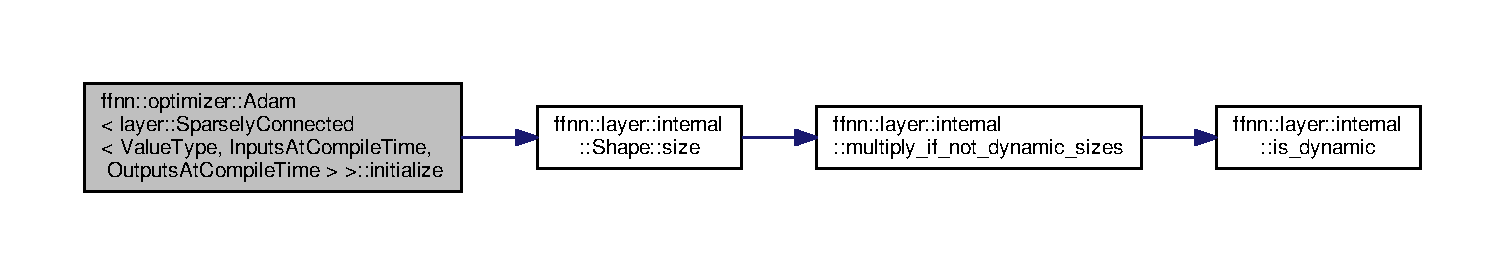
\includegraphics[width=350pt]{classffnn_1_1optimizer_1_1_adam_3_01layer_1_1_sparsely_connected_3_01_value_type_00_01_inputs_at5101e46d32858ec2169acdeede08d723_a3529c6f6fb1befc882cc3ae17c00ba5a_cgraph}
\end{center}
\end{figure}


\hypertarget{classffnn_1_1optimizer_1_1_adam_3_01layer_1_1_sparsely_connected_3_01_value_type_00_01_inputs_at5101e46d32858ec2169acdeede08d723_aaa3b2eb55a9d80d51330c132df65214b}{\index{ffnn\-::optimizer\-::\-Adam$<$ layer\-::\-Sparsely\-Connected$<$ Value\-Type, Inputs\-At\-Compile\-Time, Outputs\-At\-Compile\-Time $>$ $>$@{ffnn\-::optimizer\-::\-Adam$<$ layer\-::\-Sparsely\-Connected$<$ Value\-Type, Inputs\-At\-Compile\-Time, Outputs\-At\-Compile\-Time $>$ $>$}!update@{update}}
\index{update@{update}!ffnn::optimizer::Adam< layer::SparselyConnected< ValueType, InputsAtCompileTime, OutputsAtCompileTime > >@{ffnn\-::optimizer\-::\-Adam$<$ layer\-::\-Sparsely\-Connected$<$ Value\-Type, Inputs\-At\-Compile\-Time, Outputs\-At\-Compile\-Time $>$ $>$}}
\subsubsection[{update}]{\setlength{\rightskip}{0pt plus 5cm}bool {\bf ffnn\-::optimizer\-::\-Adam}$<$ {\bf layer\-::\-Sparsely\-Connected}$<$ Value\-Type, Inputs\-At\-Compile\-Time, Outputs\-At\-Compile\-Time $>$ $>$\-::update (
\begin{DoxyParamCaption}
\item[{{\bf Layer\-Type} \&}]{layer}
\end{DoxyParamCaption}
)\hspace{0.3cm}{\ttfamily [inline]}, {\ttfamily [virtual]}}}\label{classffnn_1_1optimizer_1_1_adam_3_01layer_1_1_sparsely_connected_3_01_value_type_00_01_inputs_at5101e46d32858ec2169acdeede08d723_aaa3b2eb55a9d80d51330c132df65214b}


Applies optimization update. 


\begin{DoxyParams}[1]{Parameters}
\mbox{\tt in,out}  & {\em layer} & Layer to optimize \\
\hline
\end{DoxyParams}

\begin{DoxyRetVals}{Return values}
{\em true} & if optimization update was applied successfully \\
\hline
{\em false} & otherwise \\
\hline
\end{DoxyRetVals}


Reimplemented from \hyperlink{classffnn_1_1optimizer_1_1_gradient_descent_3_01layer_1_1_sparsely_connected_3_01_value_type_00_e6c27913ab0d90f52f73031aa88c19bf_ada280929e93a2d12f0bc21e9077e75a1}{ffnn\-::optimizer\-::\-Gradient\-Descent$<$ layer\-::\-Sparsely\-Connected$<$ Value\-Type, Inputs\-At\-Compile\-Time, Outputs\-At\-Compile\-Time $>$ $>$}.



Here is the call graph for this function\-:
\nopagebreak
\begin{figure}[H]
\begin{center}
\leavevmode
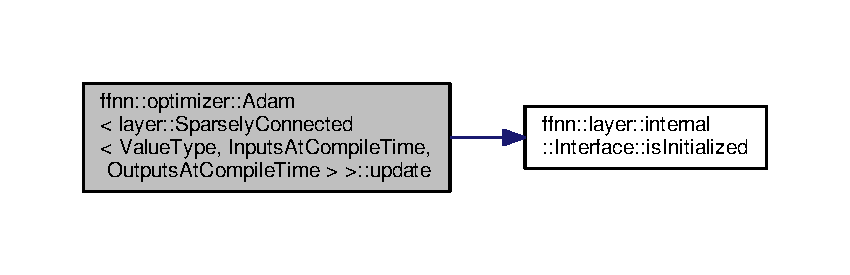
\includegraphics[width=350pt]{classffnn_1_1optimizer_1_1_adam_3_01layer_1_1_sparsely_connected_3_01_value_type_00_01_inputs_at5101e46d32858ec2169acdeede08d723_aaa3b2eb55a9d80d51330c132df65214b_cgraph}
\end{center}
\end{figure}




The documentation for this class was generated from the following file\-:\begin{DoxyCompactItemize}
\item 
/home/briancairl/packages/src/ffnn-\/cpp/ffnn/include/ffnn/optimizer/impl/adam/\hyperlink{optimizer_2impl_2adam_2sparsely__connected_8hpp}{sparsely\-\_\-connected.\-hpp}\end{DoxyCompactItemize}

\hypertarget{classffnn_1_1optimizer_1_1_adam_states}{\section{ffnn\-:\-:optimizer\-:\-:Adam\-States$<$ Value\-Type, Layer\-Type $>$ Class Template Reference}
\label{classffnn_1_1optimizer_1_1_adam_states}\index{ffnn\-::optimizer\-::\-Adam\-States$<$ Value\-Type, Layer\-Type $>$@{ffnn\-::optimizer\-::\-Adam\-States$<$ Value\-Type, Layer\-Type $>$}}
}


{\ttfamily \#include \char`\"{}adam\-\_\-states.\-hpp\char`\"{}}

\subsection*{Public Member Functions}
\begin{DoxyCompactItemize}
\item 
\hyperlink{classffnn_1_1optimizer_1_1_adam_states_a177eb4d888e9c25bc8766141f39f34e7}{Adam\-States} (Value\-Type beta1, Value\-Type beta2, Value\-Type eps)
\item 
void \hyperlink{classffnn_1_1optimizer_1_1_adam_states_a9b6ac212861f499d058a2e1c35024d57}{update} (Parameters\-Type \&gradient)
\item 
void \hyperlink{classffnn_1_1optimizer_1_1_adam_states_a8a819fc6cdb77cca470dfa6937620210}{initialize} (const Layer\-Type \&layer)
\end{DoxyCompactItemize}


\subsection{Constructor \& Destructor Documentation}
\hypertarget{classffnn_1_1optimizer_1_1_adam_states_a177eb4d888e9c25bc8766141f39f34e7}{\index{ffnn\-::optimizer\-::\-Adam\-States@{ffnn\-::optimizer\-::\-Adam\-States}!Adam\-States@{Adam\-States}}
\index{Adam\-States@{Adam\-States}!ffnn::optimizer::AdamStates@{ffnn\-::optimizer\-::\-Adam\-States}}
\subsubsection[{Adam\-States}]{\setlength{\rightskip}{0pt plus 5cm}template$<$typename Value\-Type, typename Layer\-Type$>$ {\bf ffnn\-::optimizer\-::\-Adam\-States}$<$ Value\-Type, Layer\-Type $>$\-::{\bf Adam\-States} (
\begin{DoxyParamCaption}
\item[{Value\-Type}]{beta1, }
\item[{Value\-Type}]{beta2, }
\item[{Value\-Type}]{eps}
\end{DoxyParamCaption}
)\hspace{0.3cm}{\ttfamily [inline]}}}\label{classffnn_1_1optimizer_1_1_adam_states_a177eb4d888e9c25bc8766141f39f34e7}


\subsection{Member Function Documentation}
\hypertarget{classffnn_1_1optimizer_1_1_adam_states_a8a819fc6cdb77cca470dfa6937620210}{\index{ffnn\-::optimizer\-::\-Adam\-States@{ffnn\-::optimizer\-::\-Adam\-States}!initialize@{initialize}}
\index{initialize@{initialize}!ffnn::optimizer::AdamStates@{ffnn\-::optimizer\-::\-Adam\-States}}
\subsubsection[{initialize}]{\setlength{\rightskip}{0pt plus 5cm}template$<$typename Value\-Type, typename Layer\-Type$>$ void {\bf ffnn\-::optimizer\-::\-Adam\-States}$<$ Value\-Type, Layer\-Type $>$\-::initialize (
\begin{DoxyParamCaption}
\item[{const Layer\-Type \&}]{layer}
\end{DoxyParamCaption}
)\hspace{0.3cm}{\ttfamily [inline]}}}\label{classffnn_1_1optimizer_1_1_adam_states_a8a819fc6cdb77cca470dfa6937620210}
\hypertarget{classffnn_1_1optimizer_1_1_adam_states_a9b6ac212861f499d058a2e1c35024d57}{\index{ffnn\-::optimizer\-::\-Adam\-States@{ffnn\-::optimizer\-::\-Adam\-States}!update@{update}}
\index{update@{update}!ffnn::optimizer::AdamStates@{ffnn\-::optimizer\-::\-Adam\-States}}
\subsubsection[{update}]{\setlength{\rightskip}{0pt plus 5cm}template$<$typename Value\-Type, typename Layer\-Type$>$ void {\bf ffnn\-::optimizer\-::\-Adam\-States}$<$ Value\-Type, Layer\-Type $>$\-::update (
\begin{DoxyParamCaption}
\item[{Parameters\-Type \&}]{gradient}
\end{DoxyParamCaption}
)\hspace{0.3cm}{\ttfamily [inline]}}}\label{classffnn_1_1optimizer_1_1_adam_states_a9b6ac212861f499d058a2e1c35024d57}


The documentation for this class was generated from the following file\-:\begin{DoxyCompactItemize}
\item 
/home/briancairl/packages/src/ffnn-\/cpp/ffnn/include/ffnn/impl/optimizer/adam/\hyperlink{adam__states_8hpp}{adam\-\_\-states.\-hpp}\end{DoxyCompactItemize}

\hypertarget{classffnn_1_1layer_1_1_convolution_1_1_configuration}{\section{ffnn\-:\-:layer\-:\-:Convolution$<$ Value\-Type, Options, Extrinsics $>$\-:\-:Configuration Class Reference}
\label{classffnn_1_1layer_1_1_convolution_1_1_configuration}\index{ffnn\-::layer\-::\-Convolution$<$ Value\-Type, Options, Extrinsics $>$\-::\-Configuration@{ffnn\-::layer\-::\-Convolution$<$ Value\-Type, Options, Extrinsics $>$\-::\-Configuration}}
}


\hyperlink{classffnn_1_1layer_1_1_layer}{Layer} configuration struct.  




{\ttfamily \#include \char`\"{}convolution.\-h\char`\"{}}

\subsection*{Public Member Functions}
\begin{DoxyCompactItemize}
\item 
\hyperlink{classffnn_1_1layer_1_1_convolution_1_1_configuration_a77c6503ac0920fb3147dbb0b885dcff7}{Configuration} ()
\begin{DoxyCompactList}\small\item\em Default constructor. \end{DoxyCompactList}\item 
\hyperlink{classffnn_1_1layer_1_1_convolution_1_1_configuration}{Configuration} \& \hyperlink{classffnn_1_1layer_1_1_convolution_1_1_configuration_a157b3ea8b94ae57d35771100cf247550}{set\-Optimizer} (const typename \hyperlink{classffnn_1_1optimizer_1_1_optimizer_ac03e7181934bf0c12a97fc67a60484ab}{Optimizer\-Type\-::\-Ptr} \&optimizer)
\begin{DoxyCompactList}\small\item\em Sets layer optimization resource. \end{DoxyCompactList}\item 
\hyperlink{classffnn_1_1layer_1_1_convolution_1_1_configuration}{Configuration} \& \hyperlink{classffnn_1_1layer_1_1_convolution_1_1_configuration_ae723ef56829d1788e9fc0ca44e1f7796}{set\-Parameter\-Distribution} (const typename \hyperlink{classffnn_1_1distribution_1_1_distribution_a51d4ea875b70b07862c5f68b20c8f41a}{Distribution\-Type\-::\-Ptr} \&distribution)
\begin{DoxyCompactList}\small\item\em Sets layer parameter initialization distribution. \end{DoxyCompactList}\item 
\hyperlink{classffnn_1_1layer_1_1_convolution_1_1_configuration}{Configuration} \& \hyperlink{classffnn_1_1layer_1_1_convolution_1_1_configuration_a52d8bb1768c8fac6b2fb67262c7172ec}{set\-Input\-Shape} (\hyperlink{namespaceffnn_a63b90a2fd70eb76684eac482a51633e5}{size\-\_\-type} height, \hyperlink{namespaceffnn_a63b90a2fd70eb76684eac482a51633e5}{size\-\_\-type} width, \hyperlink{namespaceffnn_a63b90a2fd70eb76684eac482a51633e5}{size\-\_\-type} depth)
\begin{DoxyCompactList}\small\item\em Sets layer input shape. \end{DoxyCompactList}\item 
\hyperlink{classffnn_1_1layer_1_1_convolution_1_1_configuration}{Configuration} \& \hyperlink{classffnn_1_1layer_1_1_convolution_1_1_configuration_acd6092bac8260ac9c9da4c11c09968d0}{set\-Filter\-Shape} (\hyperlink{namespaceffnn_a63b90a2fd70eb76684eac482a51633e5}{size\-\_\-type} height, \hyperlink{namespaceffnn_a63b90a2fd70eb76684eac482a51633e5}{size\-\_\-type} width, \hyperlink{namespaceffnn_a63b90a2fd70eb76684eac482a51633e5}{size\-\_\-type} depth)
\begin{DoxyCompactList}\small\item\em Sets layer filter shape options. \end{DoxyCompactList}\item 
\hyperlink{classffnn_1_1layer_1_1_convolution_1_1_configuration}{Configuration} \& \hyperlink{classffnn_1_1layer_1_1_convolution_1_1_configuration_af149ccc6dd80d25fefc22e57d5250c26}{set\-Stride} (\hyperlink{namespaceffnn_a63b90a2fd70eb76684eac482a51633e5}{size\-\_\-type} row\-\_\-stride, \hyperlink{namespaceffnn_a63b90a2fd70eb76684eac482a51633e5}{size\-\_\-type} col\-\_\-stride=-\/1)
\begin{DoxyCompactList}\small\item\em Sets filter stride options. \end{DoxyCompactList}\end{DoxyCompactItemize}
\subsection*{Public Attributes}
\begin{DoxyCompactItemize}
\item 
friend \hyperlink{classffnn_1_1layer_1_1_convolution_1_1_configuration_aa57a5c918311d302244afcfced552871}{Self\-Type}
\end{DoxyCompactItemize}


\subsection{Detailed Description}
\subsubsection*{template$<$typename Value\-Type, typename Options = typename convolution\-::options$<$$>$, typename Extrinsics = typename convolution\-::extrinsics$<$\-Value\-Type, Options$>$$>$class ffnn\-::layer\-::\-Convolution$<$ Value\-Type, Options, Extrinsics $>$\-::\-Configuration}

\hyperlink{classffnn_1_1layer_1_1_layer}{Layer} configuration struct. 

\subsection{Constructor \& Destructor Documentation}
\hypertarget{classffnn_1_1layer_1_1_convolution_1_1_configuration_a77c6503ac0920fb3147dbb0b885dcff7}{\index{ffnn\-::layer\-::\-Convolution\-::\-Configuration@{ffnn\-::layer\-::\-Convolution\-::\-Configuration}!Configuration@{Configuration}}
\index{Configuration@{Configuration}!ffnn::layer::Convolution::Configuration@{ffnn\-::layer\-::\-Convolution\-::\-Configuration}}
\subsubsection[{Configuration}]{\setlength{\rightskip}{0pt plus 5cm}template$<$typename Value\-Type , typename Options  = typename convolution\-::options$<$$>$, typename Extrinsics  = typename convolution\-::extrinsics$<$\-Value\-Type, Options$>$$>$ {\bf ffnn\-::layer\-::\-Convolution}$<$ Value\-Type, Options, Extrinsics $>$\-::Configuration\-::\-Configuration (
\begin{DoxyParamCaption}
{}
\end{DoxyParamCaption}
)\hspace{0.3cm}{\ttfamily [inline]}}}\label{classffnn_1_1layer_1_1_convolution_1_1_configuration_a77c6503ac0920fb3147dbb0b885dcff7}


Default constructor. 

Try to resolve from template arguments 

\subsection{Member Function Documentation}
\hypertarget{classffnn_1_1layer_1_1_convolution_1_1_configuration_acd6092bac8260ac9c9da4c11c09968d0}{\index{ffnn\-::layer\-::\-Convolution\-::\-Configuration@{ffnn\-::layer\-::\-Convolution\-::\-Configuration}!set\-Filter\-Shape@{set\-Filter\-Shape}}
\index{set\-Filter\-Shape@{set\-Filter\-Shape}!ffnn::layer::Convolution::Configuration@{ffnn\-::layer\-::\-Convolution\-::\-Configuration}}
\subsubsection[{set\-Filter\-Shape}]{\setlength{\rightskip}{0pt plus 5cm}template$<$typename Value\-Type , typename Options  = typename convolution\-::options$<$$>$, typename Extrinsics  = typename convolution\-::extrinsics$<$\-Value\-Type, Options$>$$>$ {\bf Configuration}\& {\bf ffnn\-::layer\-::\-Convolution}$<$ Value\-Type, Options, Extrinsics $>$\-::Configuration\-::set\-Filter\-Shape (
\begin{DoxyParamCaption}
\item[{{\bf size\-\_\-type}}]{height, }
\item[{{\bf size\-\_\-type}}]{width, }
\item[{{\bf size\-\_\-type}}]{depth}
\end{DoxyParamCaption}
)\hspace{0.3cm}{\ttfamily [inline]}}}\label{classffnn_1_1layer_1_1_convolution_1_1_configuration_acd6092bac8260ac9c9da4c11c09968d0}


Sets layer filter shape options. 


\begin{DoxyParams}{Parameters}
{\em height} & height of the filter kernel \\
\hline
{\em width} & width of the filter kernel \\
\hline
{\em depth} & number of kernels \\
\hline
\end{DoxyParams}
\begin{DoxyReturn}{Returns}
$\ast$this
\end{DoxyReturn}
\begin{DoxyNote}{Note}
The shape specified here is {\ttfamily (H, W, N-\/\-Kernels)}. Each kernel actually has the dimensions {\ttfamily (H, W, D)}, where {\ttfamily (D)} is the depth of the input volume 
\end{DoxyNote}
\hypertarget{classffnn_1_1layer_1_1_convolution_1_1_configuration_a52d8bb1768c8fac6b2fb67262c7172ec}{\index{ffnn\-::layer\-::\-Convolution\-::\-Configuration@{ffnn\-::layer\-::\-Convolution\-::\-Configuration}!set\-Input\-Shape@{set\-Input\-Shape}}
\index{set\-Input\-Shape@{set\-Input\-Shape}!ffnn::layer::Convolution::Configuration@{ffnn\-::layer\-::\-Convolution\-::\-Configuration}}
\subsubsection[{set\-Input\-Shape}]{\setlength{\rightskip}{0pt plus 5cm}template$<$typename Value\-Type , typename Options  = typename convolution\-::options$<$$>$, typename Extrinsics  = typename convolution\-::extrinsics$<$\-Value\-Type, Options$>$$>$ {\bf Configuration}\& {\bf ffnn\-::layer\-::\-Convolution}$<$ Value\-Type, Options, Extrinsics $>$\-::Configuration\-::set\-Input\-Shape (
\begin{DoxyParamCaption}
\item[{{\bf size\-\_\-type}}]{height, }
\item[{{\bf size\-\_\-type}}]{width, }
\item[{{\bf size\-\_\-type}}]{depth}
\end{DoxyParamCaption}
)\hspace{0.3cm}{\ttfamily [inline]}}}\label{classffnn_1_1layer_1_1_convolution_1_1_configuration_a52d8bb1768c8fac6b2fb67262c7172ec}


Sets layer input shape. 


\begin{DoxyParams}{Parameters}
{\em height} & height of the input volume \\
\hline
{\em width} & width of the input volume \\
\hline
{\em depth} & depth of the input volume \\
\hline
\end{DoxyParams}
\begin{DoxyReturn}{Returns}
$\ast$this 
\end{DoxyReturn}
\hypertarget{classffnn_1_1layer_1_1_convolution_1_1_configuration_a157b3ea8b94ae57d35771100cf247550}{\index{ffnn\-::layer\-::\-Convolution\-::\-Configuration@{ffnn\-::layer\-::\-Convolution\-::\-Configuration}!set\-Optimizer@{set\-Optimizer}}
\index{set\-Optimizer@{set\-Optimizer}!ffnn::layer::Convolution::Configuration@{ffnn\-::layer\-::\-Convolution\-::\-Configuration}}
\subsubsection[{set\-Optimizer}]{\setlength{\rightskip}{0pt plus 5cm}template$<$typename Value\-Type , typename Options  = typename convolution\-::options$<$$>$, typename Extrinsics  = typename convolution\-::extrinsics$<$\-Value\-Type, Options$>$$>$ {\bf Configuration}\& {\bf ffnn\-::layer\-::\-Convolution}$<$ Value\-Type, Options, Extrinsics $>$\-::Configuration\-::set\-Optimizer (
\begin{DoxyParamCaption}
\item[{const typename {\bf Optimizer\-Type\-::\-Ptr} \&}]{optimizer}
\end{DoxyParamCaption}
)\hspace{0.3cm}{\ttfamily [inline]}}}\label{classffnn_1_1layer_1_1_convolution_1_1_configuration_a157b3ea8b94ae57d35771100cf247550}


Sets layer optimization resource. 


\begin{DoxyParams}{Parameters}
{\em optimizer} & layer optimizer \\
\hline
\end{DoxyParams}
\begin{DoxyReturn}{Returns}
$\ast$this 
\end{DoxyReturn}
\hypertarget{classffnn_1_1layer_1_1_convolution_1_1_configuration_ae723ef56829d1788e9fc0ca44e1f7796}{\index{ffnn\-::layer\-::\-Convolution\-::\-Configuration@{ffnn\-::layer\-::\-Convolution\-::\-Configuration}!set\-Parameter\-Distribution@{set\-Parameter\-Distribution}}
\index{set\-Parameter\-Distribution@{set\-Parameter\-Distribution}!ffnn::layer::Convolution::Configuration@{ffnn\-::layer\-::\-Convolution\-::\-Configuration}}
\subsubsection[{set\-Parameter\-Distribution}]{\setlength{\rightskip}{0pt plus 5cm}template$<$typename Value\-Type , typename Options  = typename convolution\-::options$<$$>$, typename Extrinsics  = typename convolution\-::extrinsics$<$\-Value\-Type, Options$>$$>$ {\bf Configuration}\& {\bf ffnn\-::layer\-::\-Convolution}$<$ Value\-Type, Options, Extrinsics $>$\-::Configuration\-::set\-Parameter\-Distribution (
\begin{DoxyParamCaption}
\item[{const typename {\bf Distribution\-Type\-::\-Ptr} \&}]{distribution}
\end{DoxyParamCaption}
)\hspace{0.3cm}{\ttfamily [inline]}}}\label{classffnn_1_1layer_1_1_convolution_1_1_configuration_ae723ef56829d1788e9fc0ca44e1f7796}


Sets layer parameter initialization distribution. 


\begin{DoxyParams}{Parameters}
{\em distribution} & value distribution resource \\
\hline
\end{DoxyParams}
\begin{DoxyReturn}{Returns}
$\ast$this 
\end{DoxyReturn}
\hypertarget{classffnn_1_1layer_1_1_convolution_1_1_configuration_af149ccc6dd80d25fefc22e57d5250c26}{\index{ffnn\-::layer\-::\-Convolution\-::\-Configuration@{ffnn\-::layer\-::\-Convolution\-::\-Configuration}!set\-Stride@{set\-Stride}}
\index{set\-Stride@{set\-Stride}!ffnn::layer::Convolution::Configuration@{ffnn\-::layer\-::\-Convolution\-::\-Configuration}}
\subsubsection[{set\-Stride}]{\setlength{\rightskip}{0pt plus 5cm}template$<$typename Value\-Type , typename Options  = typename convolution\-::options$<$$>$, typename Extrinsics  = typename convolution\-::extrinsics$<$\-Value\-Type, Options$>$$>$ {\bf Configuration}\& {\bf ffnn\-::layer\-::\-Convolution}$<$ Value\-Type, Options, Extrinsics $>$\-::Configuration\-::set\-Stride (
\begin{DoxyParamCaption}
\item[{{\bf size\-\_\-type}}]{row\-\_\-stride, }
\item[{{\bf size\-\_\-type}}]{col\-\_\-stride = {\ttfamily -\/1}}
\end{DoxyParamCaption}
)\hspace{0.3cm}{\ttfamily [inline]}}}\label{classffnn_1_1layer_1_1_convolution_1_1_configuration_af149ccc6dd80d25fefc22e57d5250c26}


Sets filter stride options. 


\begin{DoxyParams}{Parameters}
{\em row\-\_\-stride} & filter stride along rows of input volume \\
\hline
{\em col\-\_\-stride} & filter stride along rows of input volume \par
 {\bfseries Note\-: } If {\ttfamily col\-\_\-stride} is not specified, it is defaulted to {\ttfamily row\-\_\-stride} \\
\hline
\end{DoxyParams}
\begin{DoxyReturn}{Returns}
$\ast$this 
\end{DoxyReturn}


\subsection{Member Data Documentation}
\hypertarget{classffnn_1_1layer_1_1_convolution_1_1_configuration_aa57a5c918311d302244afcfced552871}{\index{ffnn\-::layer\-::\-Convolution\-::\-Configuration@{ffnn\-::layer\-::\-Convolution\-::\-Configuration}!Self\-Type@{Self\-Type}}
\index{Self\-Type@{Self\-Type}!ffnn::layer::Convolution::Configuration@{ffnn\-::layer\-::\-Convolution\-::\-Configuration}}
\subsubsection[{Self\-Type}]{\setlength{\rightskip}{0pt plus 5cm}template$<$typename Value\-Type , typename Options  = typename convolution\-::options$<$$>$, typename Extrinsics  = typename convolution\-::extrinsics$<$\-Value\-Type, Options$>$$>$ friend {\bf ffnn\-::layer\-::\-Convolution}$<$ Value\-Type, Options, Extrinsics $>$\-::Configuration\-::\-Self\-Type}}\label{classffnn_1_1layer_1_1_convolution_1_1_configuration_aa57a5c918311d302244afcfced552871}


The documentation for this class was generated from the following file\-:\begin{DoxyCompactItemize}
\item 
/home/briancairl/packages/src/ffnn-\/cpp/ffnn/include/ffnn/layer/\hyperlink{convolution_8h}{convolution.\-h}\end{DoxyCompactItemize}

\hypertarget{classffnn_1_1layer_1_1_convolution}{\section{ffnn\-:\-:layer\-:\-:Convolution$<$ Value\-Type, Height\-At\-Compile\-Time, Width\-At\-Compile\-Time, Depth\-At\-Compile\-Time, Filter\-Height\-At\-Compile\-Time, Filter\-Width\-At\-Compile\-Time, Filter\-Count\-At\-Compile\-Time, Stride, Embedding\-Mode $>$ Class Template Reference}
\label{classffnn_1_1layer_1_1_convolution}\index{ffnn\-::layer\-::\-Convolution$<$ Value\-Type, Height\-At\-Compile\-Time, Width\-At\-Compile\-Time, Depth\-At\-Compile\-Time, Filter\-Height\-At\-Compile\-Time, Filter\-Width\-At\-Compile\-Time, Filter\-Count\-At\-Compile\-Time, Stride, Embedding\-Mode $>$@{ffnn\-::layer\-::\-Convolution$<$ Value\-Type, Height\-At\-Compile\-Time, Width\-At\-Compile\-Time, Depth\-At\-Compile\-Time, Filter\-Height\-At\-Compile\-Time, Filter\-Width\-At\-Compile\-Time, Filter\-Count\-At\-Compile\-Time, Stride, Embedding\-Mode $>$}}
}


A convolution layer.  




{\ttfamily \#include \char`\"{}convolution.\-h\char`\"{}}



Inheritance diagram for ffnn\-:\-:layer\-:\-:Convolution$<$ Value\-Type, Height\-At\-Compile\-Time, Width\-At\-Compile\-Time, Depth\-At\-Compile\-Time, Filter\-Height\-At\-Compile\-Time, Filter\-Width\-At\-Compile\-Time, Filter\-Count\-At\-Compile\-Time, Stride, Embedding\-Mode $>$\-:\nopagebreak
\begin{figure}[H]
\begin{center}
\leavevmode
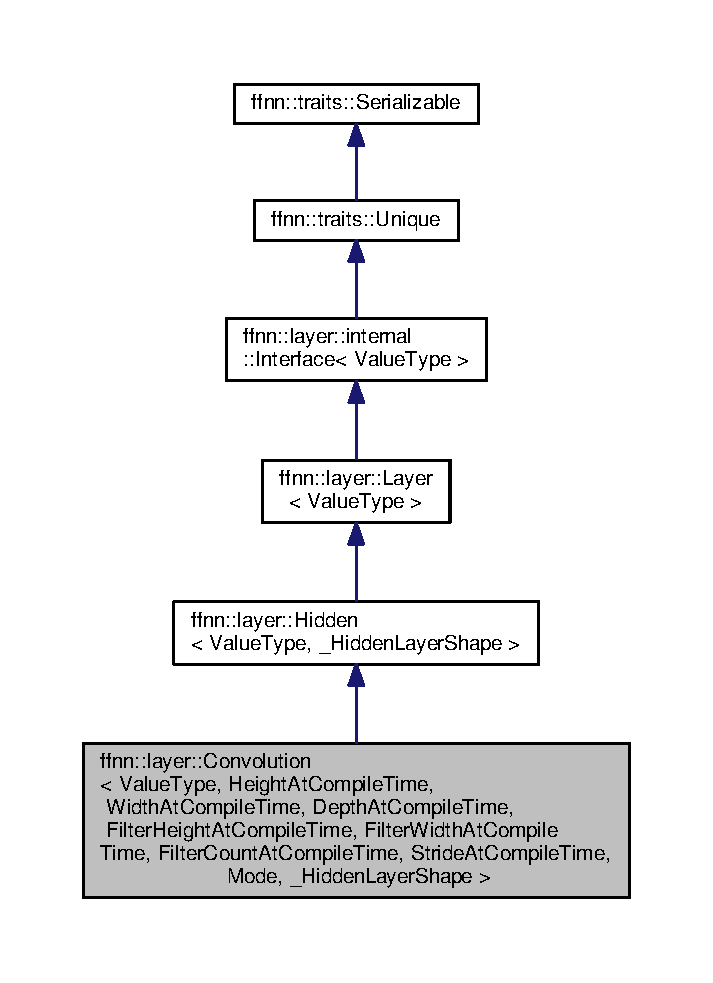
\includegraphics[width=350pt]{classffnn_1_1layer_1_1_convolution__inherit__graph}
\end{center}
\end{figure}


Collaboration diagram for ffnn\-:\-:layer\-:\-:Convolution$<$ Value\-Type, Height\-At\-Compile\-Time, Width\-At\-Compile\-Time, Depth\-At\-Compile\-Time, Filter\-Height\-At\-Compile\-Time, Filter\-Width\-At\-Compile\-Time, Filter\-Count\-At\-Compile\-Time, Stride, Embedding\-Mode $>$\-:\nopagebreak
\begin{figure}[H]
\begin{center}
\leavevmode
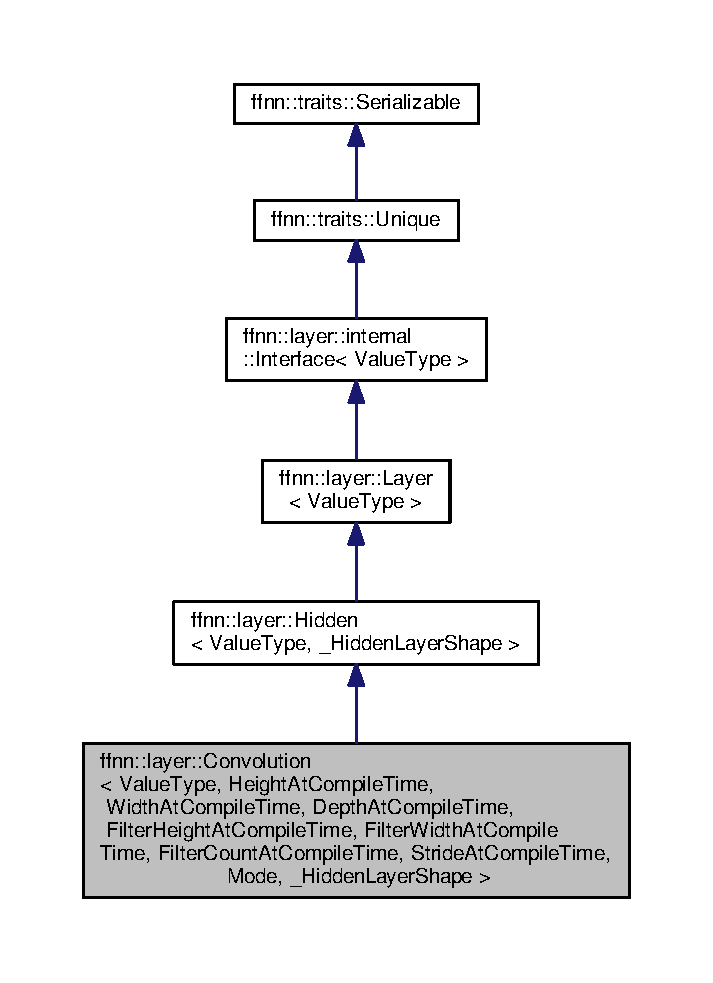
\includegraphics[width=350pt]{classffnn_1_1layer_1_1_convolution__coll__graph}
\end{center}
\end{figure}
\subsection*{Public Types}
\begin{DoxyCompactItemize}
\item 
using \hyperlink{classffnn_1_1layer_1_1_convolution_a2be75a609f983d65867bd4b5b4e27cf2}{Base} = \hyperlink{classffnn_1_1layer_1_1_hidden}{Hidden}$<$ Value\-Type, Height\-At\-Compile\-Time, Width\-At\-Compile\-Time, \hyperlink{convolution_8h_a994a9f10bc2645299b6d456cf51c7b6c}{C\-O\-N\-V\-O\-L\-U\-T\-I\-O\-N\-\_\-\-O\-U\-T\-P\-U\-T\-\_\-\-H\-E\-I\-G\-H\-T}, \hyperlink{convolution_8h_a60b63de7a979c2ced6c910f6df90356c}{C\-O\-N\-V\-O\-L\-U\-T\-I\-O\-N\-\_\-\-O\-U\-T\-P\-U\-T\-\_\-\-W\-I\-D\-T\-H} $>$
\begin{DoxyCompactList}\small\item\em Base type alias. \end{DoxyCompactList}\item 
using \hyperlink{classffnn_1_1layer_1_1_convolution_ad50136fd879d791d92c8474427fbb11f}{Self} = \hyperlink{classffnn_1_1layer_1_1_convolution}{Convolution}$<$ \hyperlink{convolution_8h_a3aee648020398150ad88775ccd534670}{C\-O\-N\-V\-O\-L\-U\-T\-I\-O\-N\-\_\-\-T\-A\-R\-G\-S} $>$
\begin{DoxyCompactList}\small\item\em Self type alias. \end{DoxyCompactList}\item 
typedef \hyperlink{classffnn_1_1layer_1_1internal_1_1_interface_a7f834e3365e5199bcbcd16d9abd63941}{Base\-::\-Scalar\-Type} \hyperlink{classffnn_1_1layer_1_1_convolution_a93ececd0b844c441245b834f05a092c4}{Scalar\-Type}
\begin{DoxyCompactList}\small\item\em Scalar type standardization. \end{DoxyCompactList}\item 
typedef \hyperlink{classffnn_1_1layer_1_1_hidden_a3deb1dc4b3a83b3d6749474debee025f}{Base\-::\-Size\-Type} \hyperlink{classffnn_1_1layer_1_1_convolution_a23ed05a9127a8fae2a0feb494d6489a4}{Size\-Type}
\begin{DoxyCompactList}\small\item\em Size type standardization. \end{DoxyCompactList}\item 
typedef \hyperlink{classffnn_1_1layer_1_1_hidden_a4a191bc002b2545231a3d80c99004693}{Base\-::\-Offset\-Type} \hyperlink{classffnn_1_1layer_1_1_convolution_ac3552ec995e5da23c32f774fa9b2f207}{Offset\-Type}
\begin{DoxyCompactList}\small\item\em Offset type standardization. \end{DoxyCompactList}\item 
typedef \hyperlink{classffnn_1_1layer_1_1_hidden_aba8b203c8b193a53d19fc26c10b14872}{Base\-::\-Dim\-Type} \hyperlink{classffnn_1_1layer_1_1_convolution_ae9e8afbc337e14a898f68d3172919764}{Dim\-Type}
\begin{DoxyCompactList}\small\item\em Dimension type standardization. \end{DoxyCompactList}\item 
typedef \hyperlink{classffnn_1_1layer_1_1_receptive_volume}{Receptive\-Volume}\\*
$<$ \hyperlink{convolution_8h_af6cd5a2c0574bdc1e2ee04974964a7ac}{C\-O\-N\-V\-O\-L\-U\-T\-I\-O\-N\-\_\-\-V\-O\-L\-U\-M\-E\-\_\-\-T\-A\-R\-G\-S} $>$ \hyperlink{classffnn_1_1layer_1_1_convolution_a6638d25b9ddddeff9359283fa40f808d}{Receptive\-Volume\-Type}
\begin{DoxyCompactList}\small\item\em Receptive-\/volume type standardization. \end{DoxyCompactList}\item 
typedef boost\-::multi\-\_\-array\\*
$<$ typename \\*
\hyperlink{classffnn_1_1layer_1_1_receptive_volume_a1c32fe58cfaa6873d328d36eada78a7f}{Receptive\-Volume\-Type\-::\-Ptr}, 2 $>$ \hyperlink{classffnn_1_1layer_1_1_convolution_a8a3ffa580341487fef94ee8cb6ee84db}{Receptive\-Volume\-Bank\-Type}
\begin{DoxyCompactList}\small\item\em Recptive-\/volume bank standardization. \end{DoxyCompactList}\item 
typedef \hyperlink{classffnn_1_1optimizer_1_1_optimizer}{optimizer\-::\-Optimizer}\\*
$<$ \hyperlink{classffnn_1_1layer_1_1_convolution_ad50136fd879d791d92c8474427fbb11f}{Self} $>$ \hyperlink{classffnn_1_1layer_1_1_convolution_ab82ec0a793b79803893489daaa9924f0}{Optimizer}
\begin{DoxyCompactList}\small\item\em \hyperlink{classffnn_1_1layer_1_1_layer}{Layer} optimization type standardization. \end{DoxyCompactList}\item 
typedef \\*
\hyperlink{structffnn_1_1layer_1_1_receptive_volume_1_1_parameters}{Receptive\-Volume\-Type\-::\-Parameters} \hyperlink{classffnn_1_1layer_1_1_convolution_a9161f9cec1bc0586c11710a1be00a0fc}{Parameters}
\begin{DoxyCompactList}\small\item\em Configuration struct type alias. \end{DoxyCompactList}\end{DoxyCompactItemize}
\subsection*{Public Member Functions}
\begin{DoxyCompactItemize}
\item 
\hyperlink{classffnn_1_1layer_1_1_convolution_af094c91b9a3d85fe5883d158930fb8ae}{Convolution} ()
\begin{DoxyCompactList}\small\item\em Setup constructor. \end{DoxyCompactList}\item 
virtual \hyperlink{classffnn_1_1layer_1_1_convolution_a4e8aa1ae4e87c216e30720910422bb86}{$\sim$\-Convolution} ()
\item 
bool \hyperlink{classffnn_1_1layer_1_1_convolution_a158af9a753113ac55730abd7b56b8684}{initialize} ()
\begin{DoxyCompactList}\small\item\em Initialize the layer. \end{DoxyCompactList}\item 
const \hyperlink{classffnn_1_1layer_1_1_convolution_a8a3ffa580341487fef94ee8cb6ee84db}{Receptive\-Volume\-Bank\-Type} \& \hyperlink{classffnn_1_1layer_1_1_convolution_a96255a17df340588fb7ae80f3b6e5b07}{get\-Receptive\-Volumes} () const 
\begin{DoxyCompactList}\small\item\em Performs forward value propagation. \end{DoxyCompactList}\end{DoxyCompactItemize}
\subsection*{Additional Inherited Members}


\subsection{Detailed Description}
\subsubsection*{template$<$typename Value\-Type, F\-F\-N\-N\-\_\-\-S\-I\-Z\-E\-\_\-\-T\-Y\-P\-E Height\-At\-Compile\-Time = Eigen\-::\-Dynamic, F\-F\-N\-N\-\_\-\-S\-I\-Z\-E\-\_\-\-T\-Y\-P\-E Width\-At\-Compile\-Time = Eigen\-::\-Dynamic, F\-F\-N\-N\-\_\-\-S\-I\-Z\-E\-\_\-\-T\-Y\-P\-E Depth\-At\-Compile\-Time = Eigen\-::\-Dynamic, F\-F\-N\-N\-\_\-\-S\-I\-Z\-E\-\_\-\-T\-Y\-P\-E Filter\-Height\-At\-Compile\-Time = Eigen\-::\-Dynamic, F\-F\-N\-N\-\_\-\-S\-I\-Z\-E\-\_\-\-T\-Y\-P\-E Filter\-Width\-At\-Compile\-Time = Eigen\-::\-Dynamic, F\-F\-N\-N\-\_\-\-S\-I\-Z\-E\-\_\-\-T\-Y\-P\-E Filter\-Count\-At\-Compile\-Time = Eigen\-::\-Dynamic, F\-F\-N\-N\-\_\-\-S\-I\-Z\-E\-\_\-\-T\-Y\-P\-E Stride = 1, F\-F\-N\-N\-\_\-\-S\-I\-Z\-E\-\_\-\-T\-Y\-P\-E Embedding\-Mode = Col\-Embedding$>$class ffnn\-::layer\-::\-Convolution$<$ Value\-Type, Height\-At\-Compile\-Time, Width\-At\-Compile\-Time, Depth\-At\-Compile\-Time, Filter\-Height\-At\-Compile\-Time, Filter\-Width\-At\-Compile\-Time, Filter\-Count\-At\-Compile\-Time, Stride, Embedding\-Mode $>$}

A convolution layer. 

\subsection{Member Typedef Documentation}
\hypertarget{classffnn_1_1layer_1_1_convolution_a2be75a609f983d65867bd4b5b4e27cf2}{\index{ffnn\-::layer\-::\-Convolution@{ffnn\-::layer\-::\-Convolution}!Base@{Base}}
\index{Base@{Base}!ffnn::layer::Convolution@{ffnn\-::layer\-::\-Convolution}}
\subsubsection[{Base}]{\setlength{\rightskip}{0pt plus 5cm}template$<$typename Value\-Type , F\-F\-N\-N\-\_\-\-S\-I\-Z\-E\-\_\-\-T\-Y\-P\-E Height\-At\-Compile\-Time = Eigen\-::\-Dynamic, F\-F\-N\-N\-\_\-\-S\-I\-Z\-E\-\_\-\-T\-Y\-P\-E Width\-At\-Compile\-Time = Eigen\-::\-Dynamic, F\-F\-N\-N\-\_\-\-S\-I\-Z\-E\-\_\-\-T\-Y\-P\-E Depth\-At\-Compile\-Time = Eigen\-::\-Dynamic, F\-F\-N\-N\-\_\-\-S\-I\-Z\-E\-\_\-\-T\-Y\-P\-E Filter\-Height\-At\-Compile\-Time = Eigen\-::\-Dynamic, F\-F\-N\-N\-\_\-\-S\-I\-Z\-E\-\_\-\-T\-Y\-P\-E Filter\-Width\-At\-Compile\-Time = Eigen\-::\-Dynamic, F\-F\-N\-N\-\_\-\-S\-I\-Z\-E\-\_\-\-T\-Y\-P\-E Filter\-Count\-At\-Compile\-Time = Eigen\-::\-Dynamic, F\-F\-N\-N\-\_\-\-S\-I\-Z\-E\-\_\-\-T\-Y\-P\-E Stride = 1, F\-F\-N\-N\-\_\-\-S\-I\-Z\-E\-\_\-\-T\-Y\-P\-E Embedding\-Mode = Col\-Embedding$>$ using {\bf ffnn\-::layer\-::\-Convolution}$<$ Value\-Type, Height\-At\-Compile\-Time, Width\-At\-Compile\-Time, Depth\-At\-Compile\-Time, Filter\-Height\-At\-Compile\-Time, Filter\-Width\-At\-Compile\-Time, Filter\-Count\-At\-Compile\-Time, Stride, {\bf Embedding\-Mode} $>$\-::{\bf Base} =  {\bf Hidden}$<$Value\-Type, Height\-At\-Compile\-Time, Width\-At\-Compile\-Time, {\bf C\-O\-N\-V\-O\-L\-U\-T\-I\-O\-N\-\_\-\-O\-U\-T\-P\-U\-T\-\_\-\-H\-E\-I\-G\-H\-T}, {\bf C\-O\-N\-V\-O\-L\-U\-T\-I\-O\-N\-\_\-\-O\-U\-T\-P\-U\-T\-\_\-\-W\-I\-D\-T\-H}$>$}}\label{classffnn_1_1layer_1_1_convolution_a2be75a609f983d65867bd4b5b4e27cf2}


Base type alias. 

\hypertarget{classffnn_1_1layer_1_1_convolution_ae9e8afbc337e14a898f68d3172919764}{\index{ffnn\-::layer\-::\-Convolution@{ffnn\-::layer\-::\-Convolution}!Dim\-Type@{Dim\-Type}}
\index{Dim\-Type@{Dim\-Type}!ffnn::layer::Convolution@{ffnn\-::layer\-::\-Convolution}}
\subsubsection[{Dim\-Type}]{\setlength{\rightskip}{0pt plus 5cm}template$<$typename Value\-Type , F\-F\-N\-N\-\_\-\-S\-I\-Z\-E\-\_\-\-T\-Y\-P\-E Height\-At\-Compile\-Time = Eigen\-::\-Dynamic, F\-F\-N\-N\-\_\-\-S\-I\-Z\-E\-\_\-\-T\-Y\-P\-E Width\-At\-Compile\-Time = Eigen\-::\-Dynamic, F\-F\-N\-N\-\_\-\-S\-I\-Z\-E\-\_\-\-T\-Y\-P\-E Depth\-At\-Compile\-Time = Eigen\-::\-Dynamic, F\-F\-N\-N\-\_\-\-S\-I\-Z\-E\-\_\-\-T\-Y\-P\-E Filter\-Height\-At\-Compile\-Time = Eigen\-::\-Dynamic, F\-F\-N\-N\-\_\-\-S\-I\-Z\-E\-\_\-\-T\-Y\-P\-E Filter\-Width\-At\-Compile\-Time = Eigen\-::\-Dynamic, F\-F\-N\-N\-\_\-\-S\-I\-Z\-E\-\_\-\-T\-Y\-P\-E Filter\-Count\-At\-Compile\-Time = Eigen\-::\-Dynamic, F\-F\-N\-N\-\_\-\-S\-I\-Z\-E\-\_\-\-T\-Y\-P\-E Stride = 1, F\-F\-N\-N\-\_\-\-S\-I\-Z\-E\-\_\-\-T\-Y\-P\-E Embedding\-Mode = Col\-Embedding$>$ typedef {\bf Base\-::\-Dim\-Type} {\bf ffnn\-::layer\-::\-Convolution}$<$ Value\-Type, Height\-At\-Compile\-Time, Width\-At\-Compile\-Time, Depth\-At\-Compile\-Time, Filter\-Height\-At\-Compile\-Time, Filter\-Width\-At\-Compile\-Time, Filter\-Count\-At\-Compile\-Time, Stride, {\bf Embedding\-Mode} $>$\-::{\bf Dim\-Type}}}\label{classffnn_1_1layer_1_1_convolution_ae9e8afbc337e14a898f68d3172919764}


Dimension type standardization. 

\hypertarget{classffnn_1_1layer_1_1_convolution_ac3552ec995e5da23c32f774fa9b2f207}{\index{ffnn\-::layer\-::\-Convolution@{ffnn\-::layer\-::\-Convolution}!Offset\-Type@{Offset\-Type}}
\index{Offset\-Type@{Offset\-Type}!ffnn::layer::Convolution@{ffnn\-::layer\-::\-Convolution}}
\subsubsection[{Offset\-Type}]{\setlength{\rightskip}{0pt plus 5cm}template$<$typename Value\-Type , F\-F\-N\-N\-\_\-\-S\-I\-Z\-E\-\_\-\-T\-Y\-P\-E Height\-At\-Compile\-Time = Eigen\-::\-Dynamic, F\-F\-N\-N\-\_\-\-S\-I\-Z\-E\-\_\-\-T\-Y\-P\-E Width\-At\-Compile\-Time = Eigen\-::\-Dynamic, F\-F\-N\-N\-\_\-\-S\-I\-Z\-E\-\_\-\-T\-Y\-P\-E Depth\-At\-Compile\-Time = Eigen\-::\-Dynamic, F\-F\-N\-N\-\_\-\-S\-I\-Z\-E\-\_\-\-T\-Y\-P\-E Filter\-Height\-At\-Compile\-Time = Eigen\-::\-Dynamic, F\-F\-N\-N\-\_\-\-S\-I\-Z\-E\-\_\-\-T\-Y\-P\-E Filter\-Width\-At\-Compile\-Time = Eigen\-::\-Dynamic, F\-F\-N\-N\-\_\-\-S\-I\-Z\-E\-\_\-\-T\-Y\-P\-E Filter\-Count\-At\-Compile\-Time = Eigen\-::\-Dynamic, F\-F\-N\-N\-\_\-\-S\-I\-Z\-E\-\_\-\-T\-Y\-P\-E Stride = 1, F\-F\-N\-N\-\_\-\-S\-I\-Z\-E\-\_\-\-T\-Y\-P\-E Embedding\-Mode = Col\-Embedding$>$ typedef {\bf Base\-::\-Offset\-Type} {\bf ffnn\-::layer\-::\-Convolution}$<$ Value\-Type, Height\-At\-Compile\-Time, Width\-At\-Compile\-Time, Depth\-At\-Compile\-Time, Filter\-Height\-At\-Compile\-Time, Filter\-Width\-At\-Compile\-Time, Filter\-Count\-At\-Compile\-Time, Stride, {\bf Embedding\-Mode} $>$\-::{\bf Offset\-Type}}}\label{classffnn_1_1layer_1_1_convolution_ac3552ec995e5da23c32f774fa9b2f207}


Offset type standardization. 

\hypertarget{classffnn_1_1layer_1_1_convolution_ab82ec0a793b79803893489daaa9924f0}{\index{ffnn\-::layer\-::\-Convolution@{ffnn\-::layer\-::\-Convolution}!Optimizer@{Optimizer}}
\index{Optimizer@{Optimizer}!ffnn::layer::Convolution@{ffnn\-::layer\-::\-Convolution}}
\subsubsection[{Optimizer}]{\setlength{\rightskip}{0pt plus 5cm}template$<$typename Value\-Type , F\-F\-N\-N\-\_\-\-S\-I\-Z\-E\-\_\-\-T\-Y\-P\-E Height\-At\-Compile\-Time = Eigen\-::\-Dynamic, F\-F\-N\-N\-\_\-\-S\-I\-Z\-E\-\_\-\-T\-Y\-P\-E Width\-At\-Compile\-Time = Eigen\-::\-Dynamic, F\-F\-N\-N\-\_\-\-S\-I\-Z\-E\-\_\-\-T\-Y\-P\-E Depth\-At\-Compile\-Time = Eigen\-::\-Dynamic, F\-F\-N\-N\-\_\-\-S\-I\-Z\-E\-\_\-\-T\-Y\-P\-E Filter\-Height\-At\-Compile\-Time = Eigen\-::\-Dynamic, F\-F\-N\-N\-\_\-\-S\-I\-Z\-E\-\_\-\-T\-Y\-P\-E Filter\-Width\-At\-Compile\-Time = Eigen\-::\-Dynamic, F\-F\-N\-N\-\_\-\-S\-I\-Z\-E\-\_\-\-T\-Y\-P\-E Filter\-Count\-At\-Compile\-Time = Eigen\-::\-Dynamic, F\-F\-N\-N\-\_\-\-S\-I\-Z\-E\-\_\-\-T\-Y\-P\-E Stride = 1, F\-F\-N\-N\-\_\-\-S\-I\-Z\-E\-\_\-\-T\-Y\-P\-E Embedding\-Mode = Col\-Embedding$>$ typedef {\bf optimizer\-::\-Optimizer}$<${\bf Self}$>$ {\bf ffnn\-::layer\-::\-Convolution}$<$ Value\-Type, Height\-At\-Compile\-Time, Width\-At\-Compile\-Time, Depth\-At\-Compile\-Time, Filter\-Height\-At\-Compile\-Time, Filter\-Width\-At\-Compile\-Time, Filter\-Count\-At\-Compile\-Time, Stride, {\bf Embedding\-Mode} $>$\-::{\bf Optimizer}}}\label{classffnn_1_1layer_1_1_convolution_ab82ec0a793b79803893489daaa9924f0}


\hyperlink{classffnn_1_1layer_1_1_layer}{Layer} optimization type standardization. 

\hypertarget{classffnn_1_1layer_1_1_convolution_a9161f9cec1bc0586c11710a1be00a0fc}{\index{ffnn\-::layer\-::\-Convolution@{ffnn\-::layer\-::\-Convolution}!Parameters@{Parameters}}
\index{Parameters@{Parameters}!ffnn::layer::Convolution@{ffnn\-::layer\-::\-Convolution}}
\subsubsection[{Parameters}]{\setlength{\rightskip}{0pt plus 5cm}template$<$typename Value\-Type , F\-F\-N\-N\-\_\-\-S\-I\-Z\-E\-\_\-\-T\-Y\-P\-E Height\-At\-Compile\-Time = Eigen\-::\-Dynamic, F\-F\-N\-N\-\_\-\-S\-I\-Z\-E\-\_\-\-T\-Y\-P\-E Width\-At\-Compile\-Time = Eigen\-::\-Dynamic, F\-F\-N\-N\-\_\-\-S\-I\-Z\-E\-\_\-\-T\-Y\-P\-E Depth\-At\-Compile\-Time = Eigen\-::\-Dynamic, F\-F\-N\-N\-\_\-\-S\-I\-Z\-E\-\_\-\-T\-Y\-P\-E Filter\-Height\-At\-Compile\-Time = Eigen\-::\-Dynamic, F\-F\-N\-N\-\_\-\-S\-I\-Z\-E\-\_\-\-T\-Y\-P\-E Filter\-Width\-At\-Compile\-Time = Eigen\-::\-Dynamic, F\-F\-N\-N\-\_\-\-S\-I\-Z\-E\-\_\-\-T\-Y\-P\-E Filter\-Count\-At\-Compile\-Time = Eigen\-::\-Dynamic, F\-F\-N\-N\-\_\-\-S\-I\-Z\-E\-\_\-\-T\-Y\-P\-E Stride = 1, F\-F\-N\-N\-\_\-\-S\-I\-Z\-E\-\_\-\-T\-Y\-P\-E Embedding\-Mode = Col\-Embedding$>$ typedef {\bf Receptive\-Volume\-Type\-::\-Parameters} {\bf ffnn\-::layer\-::\-Convolution}$<$ Value\-Type, Height\-At\-Compile\-Time, Width\-At\-Compile\-Time, Depth\-At\-Compile\-Time, Filter\-Height\-At\-Compile\-Time, Filter\-Width\-At\-Compile\-Time, Filter\-Count\-At\-Compile\-Time, Stride, {\bf Embedding\-Mode} $>$\-::{\bf Parameters}}}\label{classffnn_1_1layer_1_1_convolution_a9161f9cec1bc0586c11710a1be00a0fc}


Configuration struct type alias. 

\hypertarget{classffnn_1_1layer_1_1_convolution_a8a3ffa580341487fef94ee8cb6ee84db}{\index{ffnn\-::layer\-::\-Convolution@{ffnn\-::layer\-::\-Convolution}!Receptive\-Volume\-Bank\-Type@{Receptive\-Volume\-Bank\-Type}}
\index{Receptive\-Volume\-Bank\-Type@{Receptive\-Volume\-Bank\-Type}!ffnn::layer::Convolution@{ffnn\-::layer\-::\-Convolution}}
\subsubsection[{Receptive\-Volume\-Bank\-Type}]{\setlength{\rightskip}{0pt plus 5cm}template$<$typename Value\-Type , F\-F\-N\-N\-\_\-\-S\-I\-Z\-E\-\_\-\-T\-Y\-P\-E Height\-At\-Compile\-Time = Eigen\-::\-Dynamic, F\-F\-N\-N\-\_\-\-S\-I\-Z\-E\-\_\-\-T\-Y\-P\-E Width\-At\-Compile\-Time = Eigen\-::\-Dynamic, F\-F\-N\-N\-\_\-\-S\-I\-Z\-E\-\_\-\-T\-Y\-P\-E Depth\-At\-Compile\-Time = Eigen\-::\-Dynamic, F\-F\-N\-N\-\_\-\-S\-I\-Z\-E\-\_\-\-T\-Y\-P\-E Filter\-Height\-At\-Compile\-Time = Eigen\-::\-Dynamic, F\-F\-N\-N\-\_\-\-S\-I\-Z\-E\-\_\-\-T\-Y\-P\-E Filter\-Width\-At\-Compile\-Time = Eigen\-::\-Dynamic, F\-F\-N\-N\-\_\-\-S\-I\-Z\-E\-\_\-\-T\-Y\-P\-E Filter\-Count\-At\-Compile\-Time = Eigen\-::\-Dynamic, F\-F\-N\-N\-\_\-\-S\-I\-Z\-E\-\_\-\-T\-Y\-P\-E Stride = 1, F\-F\-N\-N\-\_\-\-S\-I\-Z\-E\-\_\-\-T\-Y\-P\-E Embedding\-Mode = Col\-Embedding$>$ typedef boost\-::multi\-\_\-array$<$typename {\bf Receptive\-Volume\-Type\-::\-Ptr}, 2$>$ {\bf ffnn\-::layer\-::\-Convolution}$<$ Value\-Type, Height\-At\-Compile\-Time, Width\-At\-Compile\-Time, Depth\-At\-Compile\-Time, Filter\-Height\-At\-Compile\-Time, Filter\-Width\-At\-Compile\-Time, Filter\-Count\-At\-Compile\-Time, Stride, {\bf Embedding\-Mode} $>$\-::{\bf Receptive\-Volume\-Bank\-Type}}}\label{classffnn_1_1layer_1_1_convolution_a8a3ffa580341487fef94ee8cb6ee84db}


Recptive-\/volume bank standardization. 

\hypertarget{classffnn_1_1layer_1_1_convolution_a6638d25b9ddddeff9359283fa40f808d}{\index{ffnn\-::layer\-::\-Convolution@{ffnn\-::layer\-::\-Convolution}!Receptive\-Volume\-Type@{Receptive\-Volume\-Type}}
\index{Receptive\-Volume\-Type@{Receptive\-Volume\-Type}!ffnn::layer::Convolution@{ffnn\-::layer\-::\-Convolution}}
\subsubsection[{Receptive\-Volume\-Type}]{\setlength{\rightskip}{0pt plus 5cm}template$<$typename Value\-Type , F\-F\-N\-N\-\_\-\-S\-I\-Z\-E\-\_\-\-T\-Y\-P\-E Height\-At\-Compile\-Time = Eigen\-::\-Dynamic, F\-F\-N\-N\-\_\-\-S\-I\-Z\-E\-\_\-\-T\-Y\-P\-E Width\-At\-Compile\-Time = Eigen\-::\-Dynamic, F\-F\-N\-N\-\_\-\-S\-I\-Z\-E\-\_\-\-T\-Y\-P\-E Depth\-At\-Compile\-Time = Eigen\-::\-Dynamic, F\-F\-N\-N\-\_\-\-S\-I\-Z\-E\-\_\-\-T\-Y\-P\-E Filter\-Height\-At\-Compile\-Time = Eigen\-::\-Dynamic, F\-F\-N\-N\-\_\-\-S\-I\-Z\-E\-\_\-\-T\-Y\-P\-E Filter\-Width\-At\-Compile\-Time = Eigen\-::\-Dynamic, F\-F\-N\-N\-\_\-\-S\-I\-Z\-E\-\_\-\-T\-Y\-P\-E Filter\-Count\-At\-Compile\-Time = Eigen\-::\-Dynamic, F\-F\-N\-N\-\_\-\-S\-I\-Z\-E\-\_\-\-T\-Y\-P\-E Stride = 1, F\-F\-N\-N\-\_\-\-S\-I\-Z\-E\-\_\-\-T\-Y\-P\-E Embedding\-Mode = Col\-Embedding$>$ typedef {\bf Receptive\-Volume}$<${\bf C\-O\-N\-V\-O\-L\-U\-T\-I\-O\-N\-\_\-\-V\-O\-L\-U\-M\-E\-\_\-\-T\-A\-R\-G\-S}$>$ {\bf ffnn\-::layer\-::\-Convolution}$<$ Value\-Type, Height\-At\-Compile\-Time, Width\-At\-Compile\-Time, Depth\-At\-Compile\-Time, Filter\-Height\-At\-Compile\-Time, Filter\-Width\-At\-Compile\-Time, Filter\-Count\-At\-Compile\-Time, Stride, {\bf Embedding\-Mode} $>$\-::{\bf Receptive\-Volume\-Type}}}\label{classffnn_1_1layer_1_1_convolution_a6638d25b9ddddeff9359283fa40f808d}


Receptive-\/volume type standardization. 

\hypertarget{classffnn_1_1layer_1_1_convolution_a93ececd0b844c441245b834f05a092c4}{\index{ffnn\-::layer\-::\-Convolution@{ffnn\-::layer\-::\-Convolution}!Scalar\-Type@{Scalar\-Type}}
\index{Scalar\-Type@{Scalar\-Type}!ffnn::layer::Convolution@{ffnn\-::layer\-::\-Convolution}}
\subsubsection[{Scalar\-Type}]{\setlength{\rightskip}{0pt plus 5cm}template$<$typename Value\-Type , F\-F\-N\-N\-\_\-\-S\-I\-Z\-E\-\_\-\-T\-Y\-P\-E Height\-At\-Compile\-Time = Eigen\-::\-Dynamic, F\-F\-N\-N\-\_\-\-S\-I\-Z\-E\-\_\-\-T\-Y\-P\-E Width\-At\-Compile\-Time = Eigen\-::\-Dynamic, F\-F\-N\-N\-\_\-\-S\-I\-Z\-E\-\_\-\-T\-Y\-P\-E Depth\-At\-Compile\-Time = Eigen\-::\-Dynamic, F\-F\-N\-N\-\_\-\-S\-I\-Z\-E\-\_\-\-T\-Y\-P\-E Filter\-Height\-At\-Compile\-Time = Eigen\-::\-Dynamic, F\-F\-N\-N\-\_\-\-S\-I\-Z\-E\-\_\-\-T\-Y\-P\-E Filter\-Width\-At\-Compile\-Time = Eigen\-::\-Dynamic, F\-F\-N\-N\-\_\-\-S\-I\-Z\-E\-\_\-\-T\-Y\-P\-E Filter\-Count\-At\-Compile\-Time = Eigen\-::\-Dynamic, F\-F\-N\-N\-\_\-\-S\-I\-Z\-E\-\_\-\-T\-Y\-P\-E Stride = 1, F\-F\-N\-N\-\_\-\-S\-I\-Z\-E\-\_\-\-T\-Y\-P\-E Embedding\-Mode = Col\-Embedding$>$ typedef {\bf Base\-::\-Scalar\-Type} {\bf ffnn\-::layer\-::\-Convolution}$<$ Value\-Type, Height\-At\-Compile\-Time, Width\-At\-Compile\-Time, Depth\-At\-Compile\-Time, Filter\-Height\-At\-Compile\-Time, Filter\-Width\-At\-Compile\-Time, Filter\-Count\-At\-Compile\-Time, Stride, {\bf Embedding\-Mode} $>$\-::{\bf Scalar\-Type}}}\label{classffnn_1_1layer_1_1_convolution_a93ececd0b844c441245b834f05a092c4}


Scalar type standardization. 

\hypertarget{classffnn_1_1layer_1_1_convolution_ad50136fd879d791d92c8474427fbb11f}{\index{ffnn\-::layer\-::\-Convolution@{ffnn\-::layer\-::\-Convolution}!Self@{Self}}
\index{Self@{Self}!ffnn::layer::Convolution@{ffnn\-::layer\-::\-Convolution}}
\subsubsection[{Self}]{\setlength{\rightskip}{0pt plus 5cm}template$<$typename Value\-Type , F\-F\-N\-N\-\_\-\-S\-I\-Z\-E\-\_\-\-T\-Y\-P\-E Height\-At\-Compile\-Time = Eigen\-::\-Dynamic, F\-F\-N\-N\-\_\-\-S\-I\-Z\-E\-\_\-\-T\-Y\-P\-E Width\-At\-Compile\-Time = Eigen\-::\-Dynamic, F\-F\-N\-N\-\_\-\-S\-I\-Z\-E\-\_\-\-T\-Y\-P\-E Depth\-At\-Compile\-Time = Eigen\-::\-Dynamic, F\-F\-N\-N\-\_\-\-S\-I\-Z\-E\-\_\-\-T\-Y\-P\-E Filter\-Height\-At\-Compile\-Time = Eigen\-::\-Dynamic, F\-F\-N\-N\-\_\-\-S\-I\-Z\-E\-\_\-\-T\-Y\-P\-E Filter\-Width\-At\-Compile\-Time = Eigen\-::\-Dynamic, F\-F\-N\-N\-\_\-\-S\-I\-Z\-E\-\_\-\-T\-Y\-P\-E Filter\-Count\-At\-Compile\-Time = Eigen\-::\-Dynamic, F\-F\-N\-N\-\_\-\-S\-I\-Z\-E\-\_\-\-T\-Y\-P\-E Stride = 1, F\-F\-N\-N\-\_\-\-S\-I\-Z\-E\-\_\-\-T\-Y\-P\-E Embedding\-Mode = Col\-Embedding$>$ using {\bf ffnn\-::layer\-::\-Convolution}$<$ Value\-Type, Height\-At\-Compile\-Time, Width\-At\-Compile\-Time, Depth\-At\-Compile\-Time, Filter\-Height\-At\-Compile\-Time, Filter\-Width\-At\-Compile\-Time, Filter\-Count\-At\-Compile\-Time, Stride, {\bf Embedding\-Mode} $>$\-::{\bf Self} =  {\bf Convolution}$<${\bf C\-O\-N\-V\-O\-L\-U\-T\-I\-O\-N\-\_\-\-T\-A\-R\-G\-S}$>$}}\label{classffnn_1_1layer_1_1_convolution_ad50136fd879d791d92c8474427fbb11f}


Self type alias. 

\hypertarget{classffnn_1_1layer_1_1_convolution_a23ed05a9127a8fae2a0feb494d6489a4}{\index{ffnn\-::layer\-::\-Convolution@{ffnn\-::layer\-::\-Convolution}!Size\-Type@{Size\-Type}}
\index{Size\-Type@{Size\-Type}!ffnn::layer::Convolution@{ffnn\-::layer\-::\-Convolution}}
\subsubsection[{Size\-Type}]{\setlength{\rightskip}{0pt plus 5cm}template$<$typename Value\-Type , F\-F\-N\-N\-\_\-\-S\-I\-Z\-E\-\_\-\-T\-Y\-P\-E Height\-At\-Compile\-Time = Eigen\-::\-Dynamic, F\-F\-N\-N\-\_\-\-S\-I\-Z\-E\-\_\-\-T\-Y\-P\-E Width\-At\-Compile\-Time = Eigen\-::\-Dynamic, F\-F\-N\-N\-\_\-\-S\-I\-Z\-E\-\_\-\-T\-Y\-P\-E Depth\-At\-Compile\-Time = Eigen\-::\-Dynamic, F\-F\-N\-N\-\_\-\-S\-I\-Z\-E\-\_\-\-T\-Y\-P\-E Filter\-Height\-At\-Compile\-Time = Eigen\-::\-Dynamic, F\-F\-N\-N\-\_\-\-S\-I\-Z\-E\-\_\-\-T\-Y\-P\-E Filter\-Width\-At\-Compile\-Time = Eigen\-::\-Dynamic, F\-F\-N\-N\-\_\-\-S\-I\-Z\-E\-\_\-\-T\-Y\-P\-E Filter\-Count\-At\-Compile\-Time = Eigen\-::\-Dynamic, F\-F\-N\-N\-\_\-\-S\-I\-Z\-E\-\_\-\-T\-Y\-P\-E Stride = 1, F\-F\-N\-N\-\_\-\-S\-I\-Z\-E\-\_\-\-T\-Y\-P\-E Embedding\-Mode = Col\-Embedding$>$ typedef {\bf Base\-::\-Size\-Type} {\bf ffnn\-::layer\-::\-Convolution}$<$ Value\-Type, Height\-At\-Compile\-Time, Width\-At\-Compile\-Time, Depth\-At\-Compile\-Time, Filter\-Height\-At\-Compile\-Time, Filter\-Width\-At\-Compile\-Time, Filter\-Count\-At\-Compile\-Time, Stride, {\bf Embedding\-Mode} $>$\-::{\bf Size\-Type}}}\label{classffnn_1_1layer_1_1_convolution_a23ed05a9127a8fae2a0feb494d6489a4}


Size type standardization. 



\subsection{Constructor \& Destructor Documentation}
\hypertarget{classffnn_1_1layer_1_1_convolution_af094c91b9a3d85fe5883d158930fb8ae}{\index{ffnn\-::layer\-::\-Convolution@{ffnn\-::layer\-::\-Convolution}!Convolution@{Convolution}}
\index{Convolution@{Convolution}!ffnn::layer::Convolution@{ffnn\-::layer\-::\-Convolution}}
\subsubsection[{Convolution}]{\setlength{\rightskip}{0pt plus 5cm}template$<$typename Value\-Type , F\-F\-N\-N\-\_\-\-S\-I\-Z\-E\-\_\-\-T\-Y\-P\-E Height\-At\-Compile\-Time = Eigen\-::\-Dynamic, F\-F\-N\-N\-\_\-\-S\-I\-Z\-E\-\_\-\-T\-Y\-P\-E Width\-At\-Compile\-Time = Eigen\-::\-Dynamic, F\-F\-N\-N\-\_\-\-S\-I\-Z\-E\-\_\-\-T\-Y\-P\-E Depth\-At\-Compile\-Time = Eigen\-::\-Dynamic, F\-F\-N\-N\-\_\-\-S\-I\-Z\-E\-\_\-\-T\-Y\-P\-E Filter\-Height\-At\-Compile\-Time = Eigen\-::\-Dynamic, F\-F\-N\-N\-\_\-\-S\-I\-Z\-E\-\_\-\-T\-Y\-P\-E Filter\-Width\-At\-Compile\-Time = Eigen\-::\-Dynamic, F\-F\-N\-N\-\_\-\-S\-I\-Z\-E\-\_\-\-T\-Y\-P\-E Filter\-Count\-At\-Compile\-Time = Eigen\-::\-Dynamic, F\-F\-N\-N\-\_\-\-S\-I\-Z\-E\-\_\-\-T\-Y\-P\-E Stride = 1, F\-F\-N\-N\-\_\-\-S\-I\-Z\-E\-\_\-\-T\-Y\-P\-E Embedding\-Mode = Col\-Embedding$>$ {\bf ffnn\-::layer\-::\-Convolution}$<$ Value\-Type, Height\-At\-Compile\-Time, Width\-At\-Compile\-Time, Depth\-At\-Compile\-Time, Filter\-Height\-At\-Compile\-Time, Filter\-Width\-At\-Compile\-Time, Filter\-Count\-At\-Compile\-Time, Stride, {\bf Embedding\-Mode} $>$\-::{\bf Convolution} (
\begin{DoxyParamCaption}
{}
\end{DoxyParamCaption}
)\hspace{0.3cm}{\ttfamily [inline]}, {\ttfamily [explicit]}}}\label{classffnn_1_1layer_1_1_convolution_af094c91b9a3d85fe5883d158930fb8ae}


Setup constructor. 


\begin{DoxyParams}{Parameters}
{\em output\-\_\-size} & number of layer outputs \\
\hline
{\em config} & layer configuration struct \\
\hline
\end{DoxyParams}
\hypertarget{classffnn_1_1layer_1_1_convolution_a4e8aa1ae4e87c216e30720910422bb86}{\index{ffnn\-::layer\-::\-Convolution@{ffnn\-::layer\-::\-Convolution}!$\sim$\-Convolution@{$\sim$\-Convolution}}
\index{$\sim$\-Convolution@{$\sim$\-Convolution}!ffnn::layer::Convolution@{ffnn\-::layer\-::\-Convolution}}
\subsubsection[{$\sim$\-Convolution}]{\setlength{\rightskip}{0pt plus 5cm}template$<$typename Value\-Type , F\-F\-N\-N\-\_\-\-S\-I\-Z\-E\-\_\-\-T\-Y\-P\-E Height\-At\-Compile\-Time = Eigen\-::\-Dynamic, F\-F\-N\-N\-\_\-\-S\-I\-Z\-E\-\_\-\-T\-Y\-P\-E Width\-At\-Compile\-Time = Eigen\-::\-Dynamic, F\-F\-N\-N\-\_\-\-S\-I\-Z\-E\-\_\-\-T\-Y\-P\-E Depth\-At\-Compile\-Time = Eigen\-::\-Dynamic, F\-F\-N\-N\-\_\-\-S\-I\-Z\-E\-\_\-\-T\-Y\-P\-E Filter\-Height\-At\-Compile\-Time = Eigen\-::\-Dynamic, F\-F\-N\-N\-\_\-\-S\-I\-Z\-E\-\_\-\-T\-Y\-P\-E Filter\-Width\-At\-Compile\-Time = Eigen\-::\-Dynamic, F\-F\-N\-N\-\_\-\-S\-I\-Z\-E\-\_\-\-T\-Y\-P\-E Filter\-Count\-At\-Compile\-Time = Eigen\-::\-Dynamic, F\-F\-N\-N\-\_\-\-S\-I\-Z\-E\-\_\-\-T\-Y\-P\-E Stride = 1, F\-F\-N\-N\-\_\-\-S\-I\-Z\-E\-\_\-\-T\-Y\-P\-E Embedding\-Mode = Col\-Embedding$>$ virtual {\bf ffnn\-::layer\-::\-Convolution}$<$ Value\-Type, Height\-At\-Compile\-Time, Width\-At\-Compile\-Time, Depth\-At\-Compile\-Time, Filter\-Height\-At\-Compile\-Time, Filter\-Width\-At\-Compile\-Time, Filter\-Count\-At\-Compile\-Time, Stride, {\bf Embedding\-Mode} $>$\-::$\sim${\bf Convolution} (
\begin{DoxyParamCaption}
{}
\end{DoxyParamCaption}
)\hspace{0.3cm}{\ttfamily [inline]}, {\ttfamily [virtual]}}}\label{classffnn_1_1layer_1_1_convolution_a4e8aa1ae4e87c216e30720910422bb86}


\subsection{Member Function Documentation}
\hypertarget{classffnn_1_1layer_1_1_convolution_a96255a17df340588fb7ae80f3b6e5b07}{\index{ffnn\-::layer\-::\-Convolution@{ffnn\-::layer\-::\-Convolution}!get\-Receptive\-Volumes@{get\-Receptive\-Volumes}}
\index{get\-Receptive\-Volumes@{get\-Receptive\-Volumes}!ffnn::layer::Convolution@{ffnn\-::layer\-::\-Convolution}}
\subsubsection[{get\-Receptive\-Volumes}]{\setlength{\rightskip}{0pt plus 5cm}template$<$typename Value\-Type , F\-F\-N\-N\-\_\-\-S\-I\-Z\-E\-\_\-\-T\-Y\-P\-E Height\-At\-Compile\-Time = Eigen\-::\-Dynamic, F\-F\-N\-N\-\_\-\-S\-I\-Z\-E\-\_\-\-T\-Y\-P\-E Width\-At\-Compile\-Time = Eigen\-::\-Dynamic, F\-F\-N\-N\-\_\-\-S\-I\-Z\-E\-\_\-\-T\-Y\-P\-E Depth\-At\-Compile\-Time = Eigen\-::\-Dynamic, F\-F\-N\-N\-\_\-\-S\-I\-Z\-E\-\_\-\-T\-Y\-P\-E Filter\-Height\-At\-Compile\-Time = Eigen\-::\-Dynamic, F\-F\-N\-N\-\_\-\-S\-I\-Z\-E\-\_\-\-T\-Y\-P\-E Filter\-Width\-At\-Compile\-Time = Eigen\-::\-Dynamic, F\-F\-N\-N\-\_\-\-S\-I\-Z\-E\-\_\-\-T\-Y\-P\-E Filter\-Count\-At\-Compile\-Time = Eigen\-::\-Dynamic, F\-F\-N\-N\-\_\-\-S\-I\-Z\-E\-\_\-\-T\-Y\-P\-E Stride = 1, F\-F\-N\-N\-\_\-\-S\-I\-Z\-E\-\_\-\-T\-Y\-P\-E Embedding\-Mode = Col\-Embedding$>$ const {\bf Receptive\-Volume\-Bank\-Type}\& {\bf ffnn\-::layer\-::\-Convolution}$<$ Value\-Type, Height\-At\-Compile\-Time, Width\-At\-Compile\-Time, Depth\-At\-Compile\-Time, Filter\-Height\-At\-Compile\-Time, Filter\-Width\-At\-Compile\-Time, Filter\-Count\-At\-Compile\-Time, Stride, {\bf Embedding\-Mode} $>$\-::get\-Receptive\-Volumes (
\begin{DoxyParamCaption}
{}
\end{DoxyParamCaption}
) const\hspace{0.3cm}{\ttfamily [inline]}}}\label{classffnn_1_1layer_1_1_convolution_a96255a17df340588fb7ae80f3b6e5b07}


Performs forward value propagation. 


\begin{DoxyRetVals}{Return values}
{\em true} & if forward-\/propagation succeeded \\
\hline
{\em false} & otherwise Performs backward error propagation \\
\hline
{\em true} & if backward-\/propagation succeeded \\
\hline
{\em false} & otherwise \\
\hline
\end{DoxyRetVals}
\begin{DoxyWarning}{Warning}
Does not apply layer weight updates 

Will throw if an optimizer has not been associated with this layer 
\end{DoxyWarning}
\begin{DoxySeeAlso}{See Also}
set\-Optimizer Applies accumulated \hyperlink{namespaceffnn_1_1layer}{layer} weight updates computed during optimization 
\end{DoxySeeAlso}

\begin{DoxyRetVals}{Return values}
{\em true} & if weight update succeeded \\
\hline
{\em false} & otherwise \\
\hline
\end{DoxyRetVals}
\begin{DoxyWarning}{Warning}
Will throw if an optimizer has not been associated with this layer 
\end{DoxyWarning}
\begin{DoxySeeAlso}{See Also}
set\-Optimizer Reset weights and biases 
\end{DoxySeeAlso}
\hypertarget{classffnn_1_1layer_1_1_convolution_a158af9a753113ac55730abd7b56b8684}{\index{ffnn\-::layer\-::\-Convolution@{ffnn\-::layer\-::\-Convolution}!initialize@{initialize}}
\index{initialize@{initialize}!ffnn::layer::Convolution@{ffnn\-::layer\-::\-Convolution}}
\subsubsection[{initialize}]{\setlength{\rightskip}{0pt plus 5cm}template$<$typename Value\-Type , F\-F\-N\-N\-\_\-\-S\-I\-Z\-E\-\_\-\-T\-Y\-P\-E Height\-At\-Compile\-Time = Eigen\-::\-Dynamic, F\-F\-N\-N\-\_\-\-S\-I\-Z\-E\-\_\-\-T\-Y\-P\-E Width\-At\-Compile\-Time = Eigen\-::\-Dynamic, F\-F\-N\-N\-\_\-\-S\-I\-Z\-E\-\_\-\-T\-Y\-P\-E Depth\-At\-Compile\-Time = Eigen\-::\-Dynamic, F\-F\-N\-N\-\_\-\-S\-I\-Z\-E\-\_\-\-T\-Y\-P\-E Filter\-Height\-At\-Compile\-Time = Eigen\-::\-Dynamic, F\-F\-N\-N\-\_\-\-S\-I\-Z\-E\-\_\-\-T\-Y\-P\-E Filter\-Width\-At\-Compile\-Time = Eigen\-::\-Dynamic, F\-F\-N\-N\-\_\-\-S\-I\-Z\-E\-\_\-\-T\-Y\-P\-E Filter\-Count\-At\-Compile\-Time = Eigen\-::\-Dynamic, F\-F\-N\-N\-\_\-\-S\-I\-Z\-E\-\_\-\-T\-Y\-P\-E Stride = 1, F\-F\-N\-N\-\_\-\-S\-I\-Z\-E\-\_\-\-T\-Y\-P\-E Embedding\-Mode = Col\-Embedding$>$ bool {\bf ffnn\-::layer\-::\-Convolution}$<$ Value\-Type, Height\-At\-Compile\-Time, Width\-At\-Compile\-Time, Depth\-At\-Compile\-Time, Filter\-Height\-At\-Compile\-Time, Filter\-Width\-At\-Compile\-Time, Filter\-Count\-At\-Compile\-Time, Stride, {\bf Embedding\-Mode} $>$\-::initialize (
\begin{DoxyParamCaption}
{}
\end{DoxyParamCaption}
)\hspace{0.3cm}{\ttfamily [inline]}, {\ttfamily [virtual]}}}\label{classffnn_1_1layer_1_1_convolution_a158af9a753113ac55730abd7b56b8684}


Initialize the layer. 



Reimplemented from \hyperlink{classffnn_1_1layer_1_1_hidden_a3b5458a771fcf2371376049d85afbc92}{ffnn\-::layer\-::\-Hidden$<$ C\-O\-N\-V\-O\-L\-U\-T\-I\-O\-N\-\_\-\-B\-A\-S\-E\-\_\-\-T\-A\-R\-G\-S $>$}.



Here is the call graph for this function\-:\nopagebreak
\begin{figure}[H]
\begin{center}
\leavevmode
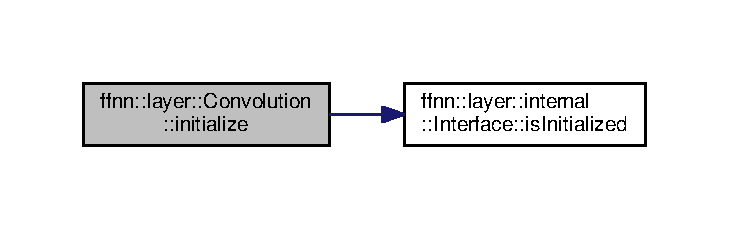
\includegraphics[width=350pt]{classffnn_1_1layer_1_1_convolution_a158af9a753113ac55730abd7b56b8684_cgraph}
\end{center}
\end{figure}




The documentation for this class was generated from the following file\-:\begin{DoxyCompactItemize}
\item 
/home/briancairl/packages/src/ffnn-\/cpp/ffnn/include/ffnn/layer/\hyperlink{convolution_8h}{convolution.\-h}\end{DoxyCompactItemize}

\hypertarget{classffnn_1_1distribution_1_1_distribution}{\section{ffnn\-:\-:distribution\-:\-:Distribution$<$ Value\-Type $>$ Class Template Reference}
\label{classffnn_1_1distribution_1_1_distribution}\index{ffnn\-::distribution\-::\-Distribution$<$ Value\-Type $>$@{ffnn\-::distribution\-::\-Distribution$<$ Value\-Type $>$}}
}


{\ttfamily \#include \char`\"{}distribution.\-h\char`\"{}}

\subsection*{Public Member Functions}
\begin{DoxyCompactItemize}
\item 
virtual Value\-Type \hyperlink{classffnn_1_1distribution_1_1_distribution_a62760bdfd46cdc21c2a7ab137b491508}{generate} ()=0
\begin{DoxyCompactList}\small\item\em Require that Value\-Type is floating point. \end{DoxyCompactList}\item 
virtual Value\-Type \hyperlink{classffnn_1_1distribution_1_1_distribution_abd2db033dd692d4b78915734c5c02204}{cdf} (const Value\-Type \&value) const =0
\begin{DoxyCompactList}\small\item\em Computes C\-D\-F of distribution at specified point. \end{DoxyCompactList}\end{DoxyCompactItemize}


\subsection{Member Function Documentation}
\hypertarget{classffnn_1_1distribution_1_1_distribution_abd2db033dd692d4b78915734c5c02204}{\index{ffnn\-::distribution\-::\-Distribution@{ffnn\-::distribution\-::\-Distribution}!cdf@{cdf}}
\index{cdf@{cdf}!ffnn::distribution::Distribution@{ffnn\-::distribution\-::\-Distribution}}
\subsubsection[{cdf}]{\setlength{\rightskip}{0pt plus 5cm}template$<$typename Value\-Type $>$ virtual Value\-Type {\bf ffnn\-::distribution\-::\-Distribution}$<$ Value\-Type $>$\-::cdf (
\begin{DoxyParamCaption}
\item[{const Value\-Type \&}]{value}
\end{DoxyParamCaption}
) const\hspace{0.3cm}{\ttfamily [pure virtual]}}}\label{classffnn_1_1distribution_1_1_distribution_abd2db033dd692d4b78915734c5c02204}


Computes C\-D\-F of distribution at specified point. 


\begin{DoxyParams}[1]{Parameters}
\mbox{\tt in}  & {\em value} & C\-D\-F upper bound \\
\hline
\end{DoxyParams}
\begin{DoxyReturn}{Returns}
cumulative probability 
\end{DoxyReturn}
\hypertarget{classffnn_1_1distribution_1_1_distribution_a62760bdfd46cdc21c2a7ab137b491508}{\index{ffnn\-::distribution\-::\-Distribution@{ffnn\-::distribution\-::\-Distribution}!generate@{generate}}
\index{generate@{generate}!ffnn::distribution::Distribution@{ffnn\-::distribution\-::\-Distribution}}
\subsubsection[{generate}]{\setlength{\rightskip}{0pt plus 5cm}template$<$typename Value\-Type $>$ virtual Value\-Type {\bf ffnn\-::distribution\-::\-Distribution}$<$ Value\-Type $>$\-::generate (
\begin{DoxyParamCaption}
{}
\end{DoxyParamCaption}
)\hspace{0.3cm}{\ttfamily [pure virtual]}}}\label{classffnn_1_1distribution_1_1_distribution_a62760bdfd46cdc21c2a7ab137b491508}


Require that Value\-Type is floating point. 

Generates a random value 
\begin{DoxyParams}[1]{Parameters}
\mbox{\tt in}  & {\em input} & a scalar input value \\
\hline
\mbox{\tt in,out}  & {\em output} & a scalar output value \\
\hline
\end{DoxyParams}


The documentation for this class was generated from the following file\-:\begin{DoxyCompactItemize}
\item 
/home/briancairl/packages/src/ffnn-\/cpp/ffnn/include/ffnn/distribution/\hyperlink{distribution_8h}{distribution.\-h}\end{DoxyCompactItemize}

\hypertarget{classffnn_1_1neuron_1_1modifier_1_1_dropout}{\section{ffnn\-:\-:neuron\-:\-:modifier\-:\-:Dropout$<$ Value\-Type, Neuron\-Type, Distribution\-Type, \-\_\-\-P, \-\_\-\-B $>$ Class Template Reference}
\label{classffnn_1_1neuron_1_1modifier_1_1_dropout}\index{ffnn\-::neuron\-::modifier\-::\-Dropout$<$ Value\-Type, Neuron\-Type, Distribution\-Type, \-\_\-\-P, \-\_\-\-B $>$@{ffnn\-::neuron\-::modifier\-::\-Dropout$<$ Value\-Type, Neuron\-Type, Distribution\-Type, \-\_\-\-P, \-\_\-\-B $>$}}
}


{\ttfamily \#include \char`\"{}dropout.\-h\char`\"{}}



Inheritance diagram for ffnn\-:\-:neuron\-:\-:modifier\-:\-:Dropout$<$ Value\-Type, Neuron\-Type, Distribution\-Type, \-\_\-\-P, \-\_\-\-B $>$\-:\nopagebreak
\begin{figure}[H]
\begin{center}
\leavevmode
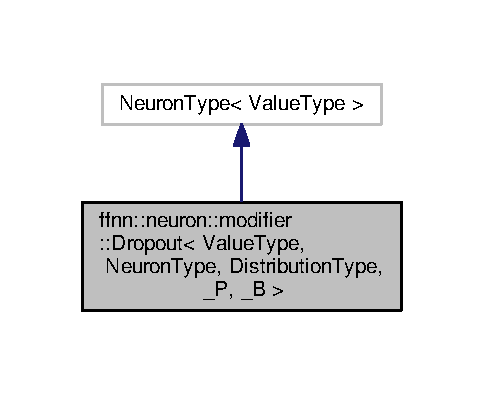
\includegraphics[width=232pt]{classffnn_1_1neuron_1_1modifier_1_1_dropout__inherit__graph}
\end{center}
\end{figure}


Collaboration diagram for ffnn\-:\-:neuron\-:\-:modifier\-:\-:Dropout$<$ Value\-Type, Neuron\-Type, Distribution\-Type, \-\_\-\-P, \-\_\-\-B $>$\-:\nopagebreak
\begin{figure}[H]
\begin{center}
\leavevmode
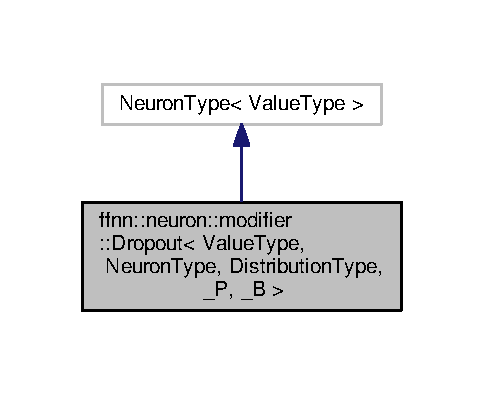
\includegraphics[width=232pt]{classffnn_1_1neuron_1_1modifier_1_1_dropout__coll__graph}
\end{center}
\end{figure}
\subsection*{Public Member Functions}
\begin{DoxyCompactItemize}
\item 
\hyperlink{classffnn_1_1neuron_1_1modifier_1_1_dropout_a0cb32cdb762c72325e291efa46c7930b}{Dropout} ()
\begin{DoxyCompactList}\small\item\em Default constructor. \end{DoxyCompactList}\item 
virtual void \hyperlink{classffnn_1_1neuron_1_1modifier_1_1_dropout_a79b58be55389a20fae9898a5a098fa3a}{operator()} (const Value\-Type \&input, Value\-Type \&output)
\begin{DoxyCompactList}\small\item\em Computes activation output. \end{DoxyCompactList}\item 
virtual void \hyperlink{classffnn_1_1neuron_1_1modifier_1_1_dropout_a5c8fc3e6fecbe9389aabbbce6abf38ba}{derivative} (const Value\-Type \&input, Value\-Type \&output) const 
\begin{DoxyCompactList}\small\item\em Computes first-\/order activation derivative. \end{DoxyCompactList}\end{DoxyCompactItemize}


\subsection{Constructor \& Destructor Documentation}
\hypertarget{classffnn_1_1neuron_1_1modifier_1_1_dropout_a0cb32cdb762c72325e291efa46c7930b}{\index{ffnn\-::neuron\-::modifier\-::\-Dropout@{ffnn\-::neuron\-::modifier\-::\-Dropout}!Dropout@{Dropout}}
\index{Dropout@{Dropout}!ffnn::neuron::modifier::Dropout@{ffnn\-::neuron\-::modifier\-::\-Dropout}}
\subsubsection[{Dropout}]{\setlength{\rightskip}{0pt plus 5cm}template$<$typename Value\-Type , template$<$ class $>$ class Neuron\-Type, template$<$ class $>$ class Distribution\-Type, F\-F\-N\-N\-\_\-\-S\-I\-Z\-E\-\_\-\-T\-Y\-P\-E \-\_\-\-P, F\-F\-N\-N\-\_\-\-S\-I\-Z\-E\-\_\-\-T\-Y\-P\-E \-\_\-\-B = 100$>$ {\bf ffnn\-::neuron\-::modifier\-::\-Dropout}$<$ Value\-Type, Neuron\-Type, Distribution\-Type, \-\_\-\-P, \-\_\-\-B $>$\-::{\bf Dropout} (
\begin{DoxyParamCaption}
{}
\end{DoxyParamCaption}
)\hspace{0.3cm}{\ttfamily [inline]}}}\label{classffnn_1_1neuron_1_1modifier_1_1_dropout_a0cb32cdb762c72325e291efa46c7930b}


Default constructor. 



\subsection{Member Function Documentation}
\hypertarget{classffnn_1_1neuron_1_1modifier_1_1_dropout_a5c8fc3e6fecbe9389aabbbce6abf38ba}{\index{ffnn\-::neuron\-::modifier\-::\-Dropout@{ffnn\-::neuron\-::modifier\-::\-Dropout}!derivative@{derivative}}
\index{derivative@{derivative}!ffnn::neuron::modifier::Dropout@{ffnn\-::neuron\-::modifier\-::\-Dropout}}
\subsubsection[{derivative}]{\setlength{\rightskip}{0pt plus 5cm}template$<$typename Value\-Type , template$<$ class $>$ class Neuron\-Type, template$<$ class $>$ class Distribution\-Type, F\-F\-N\-N\-\_\-\-S\-I\-Z\-E\-\_\-\-T\-Y\-P\-E \-\_\-\-P, F\-F\-N\-N\-\_\-\-S\-I\-Z\-E\-\_\-\-T\-Y\-P\-E \-\_\-\-B = 100$>$ virtual void {\bf ffnn\-::neuron\-::modifier\-::\-Dropout}$<$ Value\-Type, Neuron\-Type, Distribution\-Type, \-\_\-\-P, \-\_\-\-B $>$\-::derivative (
\begin{DoxyParamCaption}
\item[{const Value\-Type \&}]{input, }
\item[{Value\-Type \&}]{output}
\end{DoxyParamCaption}
) const\hspace{0.3cm}{\ttfamily [inline]}, {\ttfamily [virtual]}}}\label{classffnn_1_1neuron_1_1modifier_1_1_dropout_a5c8fc3e6fecbe9389aabbbce6abf38ba}


Computes first-\/order activation derivative. 


\begin{DoxyParams}[1]{Parameters}
\mbox{\tt in}  & {\em input} & a scalar input value \\
\hline
\mbox{\tt in,out}  & {\em output} & a scalar output value \\
\hline
\end{DoxyParams}
\hypertarget{classffnn_1_1neuron_1_1modifier_1_1_dropout_a79b58be55389a20fae9898a5a098fa3a}{\index{ffnn\-::neuron\-::modifier\-::\-Dropout@{ffnn\-::neuron\-::modifier\-::\-Dropout}!operator()@{operator()}}
\index{operator()@{operator()}!ffnn::neuron::modifier::Dropout@{ffnn\-::neuron\-::modifier\-::\-Dropout}}
\subsubsection[{operator()}]{\setlength{\rightskip}{0pt plus 5cm}template$<$typename Value\-Type , template$<$ class $>$ class Neuron\-Type, template$<$ class $>$ class Distribution\-Type, F\-F\-N\-N\-\_\-\-S\-I\-Z\-E\-\_\-\-T\-Y\-P\-E \-\_\-\-P, F\-F\-N\-N\-\_\-\-S\-I\-Z\-E\-\_\-\-T\-Y\-P\-E \-\_\-\-B = 100$>$ virtual void {\bf ffnn\-::neuron\-::modifier\-::\-Dropout}$<$ Value\-Type, Neuron\-Type, Distribution\-Type, \-\_\-\-P, \-\_\-\-B $>$\-::operator() (
\begin{DoxyParamCaption}
\item[{const Value\-Type \&}]{input, }
\item[{Value\-Type \&}]{output}
\end{DoxyParamCaption}
)\hspace{0.3cm}{\ttfamily [inline]}, {\ttfamily [virtual]}}}\label{classffnn_1_1neuron_1_1modifier_1_1_dropout_a79b58be55389a20fae9898a5a098fa3a}


Computes activation output. 


\begin{DoxyParams}[1]{Parameters}
\mbox{\tt in}  & {\em input} & a scalar input value \\
\hline
\mbox{\tt in,out}  & {\em output} & a scalar output value \\
\hline
\end{DoxyParams}


The documentation for this class was generated from the following file\-:\begin{DoxyCompactItemize}
\item 
/home/briancairl/packages/src/ffnn-\/cpp/ffnn/include/ffnn/neuron/modifier/\hyperlink{dropout_8h}{dropout.\-h}\end{DoxyCompactItemize}

\hypertarget{structffnn_1_1layer_1_1hidden_1_1extrinsics}{\section{ffnn\-:\-:layer\-:\-:hidden\-:\-:extrinsics$<$ Value\-Type, Options $>$ Struct Template Reference}
\label{structffnn_1_1layer_1_1hidden_1_1extrinsics}\index{ffnn\-::layer\-::hidden\-::extrinsics$<$ Value\-Type, Options $>$@{ffnn\-::layer\-::hidden\-::extrinsics$<$ Value\-Type, Options $>$}}
}


Describes types based on compile-\/time options.  




{\ttfamily \#include \char`\"{}hidden.\-h\char`\"{}}

\subsection*{Public Types}
\begin{DoxyCompactItemize}
\item 
typedef Eigen\-::\-Matrix\\*
$<$ Value\-Type, \\*
Options\-::input\-\_\-height, \\*
Options\-::input\-\_\-width, \\*
Options\-::input\-\_\-data\-\_\-ordering $>$ \hyperlink{structffnn_1_1layer_1_1hidden_1_1extrinsics_af5299a48a27726ba0d407ecb28890092}{Input\-Block\-Type}
\begin{DoxyCompactList}\small\item\em \hyperlink{classffnn_1_1layer_1_1_input}{Input} block type standardization. \end{DoxyCompactList}\item 
typedef Eigen\-::\-Matrix\\*
$<$ Value\-Type, \\*
Options\-::output\-\_\-height, \\*
Options\-::output\-\_\-width, \\*
Options\-::output\-\_\-data\-\_\-ordering $>$ \hyperlink{structffnn_1_1layer_1_1hidden_1_1extrinsics_ac5ca721e2e5843ddcf90351b59c4e56e}{Output\-Block\-Type}
\begin{DoxyCompactList}\small\item\em \hyperlink{classffnn_1_1layer_1_1_output}{Output} block type standardization. \end{DoxyCompactList}\item 
typedef std\-::conditional\\*
$<$ std\-::is\-\_\-floating\-\_\-point\\*
$<$ Value\-Type $>$\-::value, \\*
Eigen\-::\-Map$<$ \hyperlink{structffnn_1_1layer_1_1hidden_1_1extrinsics_af5299a48a27726ba0d407ecb28890092}{Input\-Block\-Type}, 16 $>$\\*
, Eigen\-::\-Map$<$ \hyperlink{structffnn_1_1layer_1_1hidden_1_1extrinsics_af5299a48a27726ba0d407ecb28890092}{Input\-Block\-Type} $>$\\*
 $>$\-::type \hyperlink{structffnn_1_1layer_1_1hidden_1_1extrinsics_a62256f740b1aaf253c9992d15cda7eab}{Input\-Mapping\-Type}
\begin{DoxyCompactList}\small\item\em \hyperlink{classffnn_1_1layer_1_1_input}{Input} block-\/mapping type standardization. \end{DoxyCompactList}\item 
typedef std\-::conditional\\*
$<$ std\-::is\-\_\-floating\-\_\-point\\*
$<$ Value\-Type $>$\-::value, \\*
Eigen\-::\-Map$<$ \hyperlink{structffnn_1_1layer_1_1hidden_1_1extrinsics_ac5ca721e2e5843ddcf90351b59c4e56e}{Output\-Block\-Type}, 16 $>$\\*
, Eigen\-::\-Map$<$ \hyperlink{structffnn_1_1layer_1_1hidden_1_1extrinsics_ac5ca721e2e5843ddcf90351b59c4e56e}{Output\-Block\-Type} $>$\\*
 $>$\-::type \hyperlink{structffnn_1_1layer_1_1hidden_1_1extrinsics_a886b2e28314f8641f14407a84af8132c}{Output\-Mapping\-Type}
\begin{DoxyCompactList}\small\item\em \hyperlink{classffnn_1_1layer_1_1_output}{Output} block-\/mapping type standardization. \end{DoxyCompactList}\item 
typedef \hyperlink{classffnn_1_1layer_1_1_layer}{Layer}$<$ Value\-Type $>$ \hyperlink{structffnn_1_1layer_1_1hidden_1_1extrinsics_a06f383c22ed682751b9a4cb8855da9eb}{Layer\-Type}
\begin{DoxyCompactList}\small\item\em \hyperlink{classffnn_1_1layer_1_1_layer}{Layer} (base type) standardization. \end{DoxyCompactList}\end{DoxyCompactItemize}


\subsection{Detailed Description}
\subsubsection*{template$<$typename Value\-Type, typename Options$>$struct ffnn\-::layer\-::hidden\-::extrinsics$<$ Value\-Type, Options $>$}

Describes types based on compile-\/time options. 

\subsection{Member Typedef Documentation}
\hypertarget{structffnn_1_1layer_1_1hidden_1_1extrinsics_af5299a48a27726ba0d407ecb28890092}{\index{ffnn\-::layer\-::hidden\-::extrinsics@{ffnn\-::layer\-::hidden\-::extrinsics}!Input\-Block\-Type@{Input\-Block\-Type}}
\index{Input\-Block\-Type@{Input\-Block\-Type}!ffnn::layer::hidden::extrinsics@{ffnn\-::layer\-::hidden\-::extrinsics}}
\subsubsection[{Input\-Block\-Type}]{\setlength{\rightskip}{0pt plus 5cm}template$<$typename Value\-Type, typename Options$>$ typedef Eigen\-::\-Matrix$<$ Value\-Type, Options\-::input\-\_\-height, Options\-::input\-\_\-width, Options\-::input\-\_\-data\-\_\-ordering $>$ {\bf ffnn\-::layer\-::hidden\-::extrinsics}$<$ Value\-Type, Options $>$\-::{\bf Input\-Block\-Type}}}\label{structffnn_1_1layer_1_1hidden_1_1extrinsics_af5299a48a27726ba0d407ecb28890092}


\hyperlink{classffnn_1_1layer_1_1_input}{Input} block type standardization. 

\hypertarget{structffnn_1_1layer_1_1hidden_1_1extrinsics_a62256f740b1aaf253c9992d15cda7eab}{\index{ffnn\-::layer\-::hidden\-::extrinsics@{ffnn\-::layer\-::hidden\-::extrinsics}!Input\-Mapping\-Type@{Input\-Mapping\-Type}}
\index{Input\-Mapping\-Type@{Input\-Mapping\-Type}!ffnn::layer::hidden::extrinsics@{ffnn\-::layer\-::hidden\-::extrinsics}}
\subsubsection[{Input\-Mapping\-Type}]{\setlength{\rightskip}{0pt plus 5cm}template$<$typename Value\-Type, typename Options$>$ typedef std\-::conditional$<$ std\-::is\-\_\-floating\-\_\-point$<$Value\-Type$>$\-::value, Eigen\-::\-Map$<${\bf Input\-Block\-Type}, 16$>$, Eigen\-::\-Map$<${\bf Input\-Block\-Type}$>$ $>$\-::type {\bf ffnn\-::layer\-::hidden\-::extrinsics}$<$ Value\-Type, Options $>$\-::{\bf Input\-Mapping\-Type}}}\label{structffnn_1_1layer_1_1hidden_1_1extrinsics_a62256f740b1aaf253c9992d15cda7eab}


\hyperlink{classffnn_1_1layer_1_1_input}{Input} block-\/mapping type standardization. 

\hypertarget{structffnn_1_1layer_1_1hidden_1_1extrinsics_a06f383c22ed682751b9a4cb8855da9eb}{\index{ffnn\-::layer\-::hidden\-::extrinsics@{ffnn\-::layer\-::hidden\-::extrinsics}!Layer\-Type@{Layer\-Type}}
\index{Layer\-Type@{Layer\-Type}!ffnn::layer::hidden::extrinsics@{ffnn\-::layer\-::hidden\-::extrinsics}}
\subsubsection[{Layer\-Type}]{\setlength{\rightskip}{0pt plus 5cm}template$<$typename Value\-Type, typename Options$>$ typedef {\bf Layer}$<$Value\-Type$>$ {\bf ffnn\-::layer\-::hidden\-::extrinsics}$<$ Value\-Type, Options $>$\-::{\bf Layer\-Type}}}\label{structffnn_1_1layer_1_1hidden_1_1extrinsics_a06f383c22ed682751b9a4cb8855da9eb}


\hyperlink{classffnn_1_1layer_1_1_layer}{Layer} (base type) standardization. 

\hypertarget{structffnn_1_1layer_1_1hidden_1_1extrinsics_ac5ca721e2e5843ddcf90351b59c4e56e}{\index{ffnn\-::layer\-::hidden\-::extrinsics@{ffnn\-::layer\-::hidden\-::extrinsics}!Output\-Block\-Type@{Output\-Block\-Type}}
\index{Output\-Block\-Type@{Output\-Block\-Type}!ffnn::layer::hidden::extrinsics@{ffnn\-::layer\-::hidden\-::extrinsics}}
\subsubsection[{Output\-Block\-Type}]{\setlength{\rightskip}{0pt plus 5cm}template$<$typename Value\-Type, typename Options$>$ typedef Eigen\-::\-Matrix$<$ Value\-Type, Options\-::output\-\_\-height, Options\-::output\-\_\-width, Options\-::output\-\_\-data\-\_\-ordering $>$ {\bf ffnn\-::layer\-::hidden\-::extrinsics}$<$ Value\-Type, Options $>$\-::{\bf Output\-Block\-Type}}}\label{structffnn_1_1layer_1_1hidden_1_1extrinsics_ac5ca721e2e5843ddcf90351b59c4e56e}


\hyperlink{classffnn_1_1layer_1_1_output}{Output} block type standardization. 

\hypertarget{structffnn_1_1layer_1_1hidden_1_1extrinsics_a886b2e28314f8641f14407a84af8132c}{\index{ffnn\-::layer\-::hidden\-::extrinsics@{ffnn\-::layer\-::hidden\-::extrinsics}!Output\-Mapping\-Type@{Output\-Mapping\-Type}}
\index{Output\-Mapping\-Type@{Output\-Mapping\-Type}!ffnn::layer::hidden::extrinsics@{ffnn\-::layer\-::hidden\-::extrinsics}}
\subsubsection[{Output\-Mapping\-Type}]{\setlength{\rightskip}{0pt plus 5cm}template$<$typename Value\-Type, typename Options$>$ typedef std\-::conditional$<$ std\-::is\-\_\-floating\-\_\-point$<$Value\-Type$>$\-::value, Eigen\-::\-Map$<${\bf Output\-Block\-Type}, 16$>$, Eigen\-::\-Map$<${\bf Output\-Block\-Type}$>$ $>$\-::type {\bf ffnn\-::layer\-::hidden\-::extrinsics}$<$ Value\-Type, Options $>$\-::{\bf Output\-Mapping\-Type}}}\label{structffnn_1_1layer_1_1hidden_1_1extrinsics_a886b2e28314f8641f14407a84af8132c}


\hyperlink{classffnn_1_1layer_1_1_output}{Output} block-\/mapping type standardization. 



The documentation for this struct was generated from the following file\-:\begin{DoxyCompactItemize}
\item 
/home/briancairl/packages/src/ffnn-\/cpp/ffnn/include/ffnn/layer/\hyperlink{hidden_8h}{hidden.\-h}\end{DoxyCompactItemize}

\hypertarget{structffnn_1_1layer_1_1convolution_1_1filter_1_1extrinsics}{\section{ffnn\-:\-:layer\-:\-:convolution\-:\-:filter\-:\-:extrinsics$<$ Value\-Type, Options $>$ Struct Template Reference}
\label{structffnn_1_1layer_1_1convolution_1_1filter_1_1extrinsics}\index{ffnn\-::layer\-::convolution\-::filter\-::extrinsics$<$ Value\-Type, Options $>$@{ffnn\-::layer\-::convolution\-::filter\-::extrinsics$<$ Value\-Type, Options $>$}}
}


Describes types based on compile-\/time options.  




{\ttfamily \#include \char`\"{}filter.\-h\char`\"{}}

\subsection*{Public Types}
\begin{DoxyCompactItemize}
\item 
typedef Eigen\-::\-Matrix\\*
$<$ Value\-Type, \\*
Options\-::embedded\-\_\-kernel\-\_\-height, \\*
Options\-::embedded\-\_\-kernel\-\_\-width, \\*
\hyperlink{namespaceffnn_1_1layer_1_1convolution_a88d0a4ec4a7dbc89c35ce95d859a78cf}{embed\-\_\-data\-\_\-order}\\*
$<$ Options\-::embedding\-\_\-mode $>$) $>$ \hyperlink{structffnn_1_1layer_1_1convolution_1_1filter_1_1extrinsics_a0b687a9387270004cdaa00c19bef26da}{Kernel\-Type}
\begin{DoxyCompactList}\small\item\em Kernel type standardization. \end{DoxyCompactList}\item 
typedef std\-::conditional\\*
$<$ Options\-::has\-\_\-fixed\-\_\-kernel\-\_\-count, \\*
std\-::array$<$ \hyperlink{structffnn_1_1layer_1_1convolution_1_1filter_1_1extrinsics_a0b687a9387270004cdaa00c19bef26da}{Kernel\-Type}, \\*
Options\-::kernel\-\_\-count $>$\\*
, typename std\-::conditional\\*
$<$ \hyperlink{structffnn_1_1internal_1_1traits_1_1is__alignable__128}{internal\-::traits\-::is\-\_\-alignable\-\_\-128}\\*
$<$ \hyperlink{structffnn_1_1layer_1_1convolution_1_1filter_1_1extrinsics_a0b687a9387270004cdaa00c19bef26da}{Kernel\-Type} $>$\-::value, \\*
std\-::vector$<$ \hyperlink{structffnn_1_1layer_1_1convolution_1_1filter_1_1extrinsics_a0b687a9387270004cdaa00c19bef26da}{Kernel\-Type}, \\*
Eigen\-::aligned\-\_\-allocator\\*
$<$ \hyperlink{structffnn_1_1layer_1_1convolution_1_1filter_1_1extrinsics_a0b687a9387270004cdaa00c19bef26da}{Kernel\-Type} $>$ $>$, std\-::vector\\*
$<$ \hyperlink{structffnn_1_1layer_1_1convolution_1_1filter_1_1extrinsics_a0b687a9387270004cdaa00c19bef26da}{Kernel\-Type} $>$ $>$\-::type $>$\-::type \hyperlink{structffnn_1_1layer_1_1convolution_1_1filter_1_1extrinsics_aa033ddfd5dc48de1253f1071211990e3}{Filter\-Base\-Type}
\begin{DoxyCompactList}\small\item\em Base type standardization. \end{DoxyCompactList}\end{DoxyCompactItemize}


\subsection{Detailed Description}
\subsubsection*{template$<$typename Value\-Type, typename Options$>$struct ffnn\-::layer\-::convolution\-::filter\-::extrinsics$<$ Value\-Type, Options $>$}

Describes types based on compile-\/time options. 

\subsection{Member Typedef Documentation}
\hypertarget{structffnn_1_1layer_1_1convolution_1_1filter_1_1extrinsics_aa033ddfd5dc48de1253f1071211990e3}{\index{ffnn\-::layer\-::convolution\-::filter\-::extrinsics@{ffnn\-::layer\-::convolution\-::filter\-::extrinsics}!Filter\-Base\-Type@{Filter\-Base\-Type}}
\index{Filter\-Base\-Type@{Filter\-Base\-Type}!ffnn::layer::convolution::filter::extrinsics@{ffnn\-::layer\-::convolution\-::filter\-::extrinsics}}
\subsubsection[{Filter\-Base\-Type}]{\setlength{\rightskip}{0pt plus 5cm}template$<$typename Value\-Type , typename Options $>$ typedef std\-::conditional$<$ Options\-::has\-\_\-fixed\-\_\-kernel\-\_\-count, std\-::array$<${\bf Kernel\-Type}, Options\-::kernel\-\_\-count$>$, typename std\-::conditional$<$ {\bf internal\-::traits\-::is\-\_\-alignable\-\_\-128}$<${\bf Kernel\-Type}$>$\-::value, std\-::vector$<${\bf Kernel\-Type}, Eigen\-::aligned\-\_\-allocator$<${\bf Kernel\-Type}$>$ $>$, std\-::vector$<${\bf Kernel\-Type}$>$ $>$\-::type $>$\-::type {\bf ffnn\-::layer\-::convolution\-::filter\-::extrinsics}$<$ Value\-Type, Options $>$\-::{\bf Filter\-Base\-Type}}}\label{structffnn_1_1layer_1_1convolution_1_1filter_1_1extrinsics_aa033ddfd5dc48de1253f1071211990e3}


Base type standardization. 

\hypertarget{structffnn_1_1layer_1_1convolution_1_1filter_1_1extrinsics_a0b687a9387270004cdaa00c19bef26da}{\index{ffnn\-::layer\-::convolution\-::filter\-::extrinsics@{ffnn\-::layer\-::convolution\-::filter\-::extrinsics}!Kernel\-Type@{Kernel\-Type}}
\index{Kernel\-Type@{Kernel\-Type}!ffnn::layer::convolution::filter::extrinsics@{ffnn\-::layer\-::convolution\-::filter\-::extrinsics}}
\subsubsection[{Kernel\-Type}]{\setlength{\rightskip}{0pt plus 5cm}template$<$typename Value\-Type , typename Options $>$ typedef Eigen\-::\-Matrix$<$ Value\-Type, Options\-::embedded\-\_\-kernel\-\_\-height, Options\-::embedded\-\_\-kernel\-\_\-width, {\bf embed\-\_\-data\-\_\-order}$<$Options\-::embedding\-\_\-mode$>$) $>$ {\bf ffnn\-::layer\-::convolution\-::filter\-::extrinsics}$<$ Value\-Type, Options $>$\-::{\bf Kernel\-Type}}}\label{structffnn_1_1layer_1_1convolution_1_1filter_1_1extrinsics_a0b687a9387270004cdaa00c19bef26da}


Kernel type standardization. 



The documentation for this struct was generated from the following file\-:\begin{DoxyCompactItemize}
\item 
/home/briancairl/packages/src/ffnn-\/cpp/ffnn/include/ffnn/layer/convolution/\hyperlink{filter_8h}{filter.\-h}\end{DoxyCompactItemize}

\hypertarget{structffnn_1_1layer_1_1convolution_1_1extrinsics}{\section{ffnn\-:\-:layer\-:\-:convolution\-:\-:extrinsics$<$ Value\-Type, Options $>$ Struct Template Reference}
\label{structffnn_1_1layer_1_1convolution_1_1extrinsics}\index{ffnn\-::layer\-::convolution\-::extrinsics$<$ Value\-Type, Options $>$@{ffnn\-::layer\-::convolution\-::extrinsics$<$ Value\-Type, Options $>$}}
}


Describes types based on compile-\/time options.  




{\ttfamily \#include \char`\"{}compile\-\_\-time\-\_\-options.\-h\char`\"{}}

\subsection*{Public Types}
\begin{DoxyCompactItemize}
\item 
typedef boost\-::multi\-\_\-array\\*
$<$ Value\-Type $\ast$, 2 $>$ \hyperlink{structffnn_1_1layer_1_1convolution_1_1extrinsics_ac75346616a5d8766c52ccf663bd97170}{Forward\-Mapping\-Grid\-Type}
\begin{DoxyCompactList}\small\item\em 2\-D-\/value mapping standardization \end{DoxyCompactList}\item 
typedef \hyperlink{structffnn_1_1layer_1_1convolution_1_1filter_1_1options}{filter\-::options}\\*
$<$ Options\-::kernel\-\_\-height, \\*
Options\-::kernel\-\_\-width, \\*
Options\-::input\-\_\-depth, \\*
Options\-::kernel\-\_\-count, \\*
Options\-::embedding\-\_\-mode $>$ \hyperlink{structffnn_1_1layer_1_1convolution_1_1extrinsics_a0de5368aa5d42881cfd7406cc2762bc5}{Filter\-Options}
\begin{DoxyCompactList}\small\item\em \hyperlink{classffnn_1_1layer_1_1convolution_1_1_filter}{Filter} traits type standardization. \end{DoxyCompactList}\item 
typedef \hyperlink{classffnn_1_1layer_1_1convolution_1_1_filter}{Filter}$<$ Value\-Type, \\*
\hyperlink{structffnn_1_1layer_1_1convolution_1_1extrinsics_a0de5368aa5d42881cfd7406cc2762bc5}{Filter\-Options} $>$ \hyperlink{structffnn_1_1layer_1_1convolution_1_1extrinsics_a7f09ed7d5f347efd854649ac8ac22e21}{Parameters\-Type}
\begin{DoxyCompactList}\small\item\em Parameters type standardization. \end{DoxyCompactList}\item 
typedef \hyperlink{structffnn_1_1layer_1_1hidden_1_1options}{hidden\-::options}\\*
$<$ Options\-::embedded\-\_\-input\-\_\-height, \\*
Options\-::embedded\-\_\-input\-\_\-width, \\*
Options\-::embedded\-\_\-output\-\_\-height, \\*
Options\-::embedded\-\_\-output\-\_\-width, \\*
\hyperlink{namespaceffnn_1_1layer_1_1convolution_a88d0a4ec4a7dbc89c35ce95d859a78cf}{embed\-\_\-data\-\_\-order}\\*
$<$ Options\-::embedding\-\_\-mode $>$\\*
), \hyperlink{namespaceffnn_1_1layer_1_1convolution_a88d0a4ec4a7dbc89c35ce95d859a78cf}{embed\-\_\-data\-\_\-order}\\*
$<$ Options\-::embedding\-\_\-mode $>$) $>$ \hyperlink{structffnn_1_1layer_1_1convolution_1_1extrinsics_a301768029fa1eb16a28981139c8122ce}{Hidden\-Layer\-Options}
\begin{DoxyCompactList}\small\item\em Compile-\/time \hyperlink{classffnn_1_1layer_1_1_hidden}{Hidden} layer traits. \end{DoxyCompactList}\item 
typedef \hyperlink{classffnn_1_1layer_1_1_hidden}{Hidden}$<$ Value\-Type, \\*
\hyperlink{structffnn_1_1layer_1_1convolution_1_1extrinsics_a301768029fa1eb16a28981139c8122ce}{Hidden\-Layer\-Options} $>$ \hyperlink{structffnn_1_1layer_1_1convolution_1_1extrinsics_a92f9ad843e8bb328d35604bdb4d6c87f}{Hidden\-Layer\-Type}
\begin{DoxyCompactList}\small\item\em \hyperlink{classffnn_1_1layer_1_1_hidden}{Hidden} layer (base type) standardization. \end{DoxyCompactList}\end{DoxyCompactItemize}


\subsection{Detailed Description}
\subsubsection*{template$<$typename Value\-Type, typename Options$>$struct ffnn\-::layer\-::convolution\-::extrinsics$<$ Value\-Type, Options $>$}

Describes types based on compile-\/time options. 

\subsection{Member Typedef Documentation}
\hypertarget{structffnn_1_1layer_1_1convolution_1_1extrinsics_a0de5368aa5d42881cfd7406cc2762bc5}{\index{ffnn\-::layer\-::convolution\-::extrinsics@{ffnn\-::layer\-::convolution\-::extrinsics}!Filter\-Options@{Filter\-Options}}
\index{Filter\-Options@{Filter\-Options}!ffnn::layer::convolution::extrinsics@{ffnn\-::layer\-::convolution\-::extrinsics}}
\subsubsection[{Filter\-Options}]{\setlength{\rightskip}{0pt plus 5cm}template$<$typename Value\-Type , typename Options $>$ typedef {\bf filter\-::options}$<$ Options\-::kernel\-\_\-height, Options\-::kernel\-\_\-width, Options\-::input\-\_\-depth, Options\-::kernel\-\_\-count, Options\-::embedding\-\_\-mode $>$ {\bf ffnn\-::layer\-::convolution\-::extrinsics}$<$ Value\-Type, Options $>$\-::{\bf Filter\-Options}}}\label{structffnn_1_1layer_1_1convolution_1_1extrinsics_a0de5368aa5d42881cfd7406cc2762bc5}


\hyperlink{classffnn_1_1layer_1_1convolution_1_1_filter}{Filter} traits type standardization. 

\hypertarget{structffnn_1_1layer_1_1convolution_1_1extrinsics_ac75346616a5d8766c52ccf663bd97170}{\index{ffnn\-::layer\-::convolution\-::extrinsics@{ffnn\-::layer\-::convolution\-::extrinsics}!Forward\-Mapping\-Grid\-Type@{Forward\-Mapping\-Grid\-Type}}
\index{Forward\-Mapping\-Grid\-Type@{Forward\-Mapping\-Grid\-Type}!ffnn::layer::convolution::extrinsics@{ffnn\-::layer\-::convolution\-::extrinsics}}
\subsubsection[{Forward\-Mapping\-Grid\-Type}]{\setlength{\rightskip}{0pt plus 5cm}template$<$typename Value\-Type , typename Options $>$ typedef boost\-::multi\-\_\-array$<$Value\-Type$\ast$, 2$>$ {\bf ffnn\-::layer\-::convolution\-::extrinsics}$<$ Value\-Type, Options $>$\-::{\bf Forward\-Mapping\-Grid\-Type}}}\label{structffnn_1_1layer_1_1convolution_1_1extrinsics_ac75346616a5d8766c52ccf663bd97170}


2\-D-\/value mapping standardization 

\hypertarget{structffnn_1_1layer_1_1convolution_1_1extrinsics_a301768029fa1eb16a28981139c8122ce}{\index{ffnn\-::layer\-::convolution\-::extrinsics@{ffnn\-::layer\-::convolution\-::extrinsics}!Hidden\-Layer\-Options@{Hidden\-Layer\-Options}}
\index{Hidden\-Layer\-Options@{Hidden\-Layer\-Options}!ffnn::layer::convolution::extrinsics@{ffnn\-::layer\-::convolution\-::extrinsics}}
\subsubsection[{Hidden\-Layer\-Options}]{\setlength{\rightskip}{0pt plus 5cm}template$<$typename Value\-Type , typename Options $>$ typedef {\bf hidden\-::options}$<$ Options\-::embedded\-\_\-input\-\_\-height, Options\-::embedded\-\_\-input\-\_\-width, Options\-::embedded\-\_\-output\-\_\-height, Options\-::embedded\-\_\-output\-\_\-width, {\bf embed\-\_\-data\-\_\-order}$<$Options\-::embedding\-\_\-mode$>$), {\bf embed\-\_\-data\-\_\-order}$<$Options\-::embedding\-\_\-mode$>$) $>$ {\bf ffnn\-::layer\-::convolution\-::extrinsics}$<$ Value\-Type, Options $>$\-::{\bf Hidden\-Layer\-Options}}}\label{structffnn_1_1layer_1_1convolution_1_1extrinsics_a301768029fa1eb16a28981139c8122ce}


Compile-\/time \hyperlink{classffnn_1_1layer_1_1_hidden}{Hidden} layer traits. 

\hypertarget{structffnn_1_1layer_1_1convolution_1_1extrinsics_a92f9ad843e8bb328d35604bdb4d6c87f}{\index{ffnn\-::layer\-::convolution\-::extrinsics@{ffnn\-::layer\-::convolution\-::extrinsics}!Hidden\-Layer\-Type@{Hidden\-Layer\-Type}}
\index{Hidden\-Layer\-Type@{Hidden\-Layer\-Type}!ffnn::layer::convolution::extrinsics@{ffnn\-::layer\-::convolution\-::extrinsics}}
\subsubsection[{Hidden\-Layer\-Type}]{\setlength{\rightskip}{0pt plus 5cm}template$<$typename Value\-Type , typename Options $>$ typedef {\bf Hidden}$<$Value\-Type, {\bf Hidden\-Layer\-Options}$>$ {\bf ffnn\-::layer\-::convolution\-::extrinsics}$<$ Value\-Type, Options $>$\-::{\bf Hidden\-Layer\-Type}}}\label{structffnn_1_1layer_1_1convolution_1_1extrinsics_a92f9ad843e8bb328d35604bdb4d6c87f}


\hyperlink{classffnn_1_1layer_1_1_hidden}{Hidden} layer (base type) standardization. 

\hypertarget{structffnn_1_1layer_1_1convolution_1_1extrinsics_a7f09ed7d5f347efd854649ac8ac22e21}{\index{ffnn\-::layer\-::convolution\-::extrinsics@{ffnn\-::layer\-::convolution\-::extrinsics}!Parameters\-Type@{Parameters\-Type}}
\index{Parameters\-Type@{Parameters\-Type}!ffnn::layer::convolution::extrinsics@{ffnn\-::layer\-::convolution\-::extrinsics}}
\subsubsection[{Parameters\-Type}]{\setlength{\rightskip}{0pt plus 5cm}template$<$typename Value\-Type , typename Options $>$ typedef {\bf Filter}$<$Value\-Type, {\bf Filter\-Options}$>$ {\bf ffnn\-::layer\-::convolution\-::extrinsics}$<$ Value\-Type, Options $>$\-::{\bf Parameters\-Type}}}\label{structffnn_1_1layer_1_1convolution_1_1extrinsics_a7f09ed7d5f347efd854649ac8ac22e21}


Parameters type standardization. 



The documentation for this struct was generated from the following file\-:\begin{DoxyCompactItemize}
\item 
/home/briancairl/packages/src/ffnn-\/cpp/ffnn/include/ffnn/layer/convolution/\hyperlink{convolution_2compile__time__options_8h}{compile\-\_\-time\-\_\-options.\-h}\end{DoxyCompactItemize}

\hypertarget{structffnn_1_1layer_1_1convolution_1_1_filter}{\section{ffnn\-:\-:layer\-:\-:convolution\-:\-:Filter$<$ Value\-Type, Options, Extrinsics $>$ Struct Template Reference}
\label{structffnn_1_1layer_1_1convolution_1_1_filter}\index{ffnn\-::layer\-::convolution\-::\-Filter$<$ Value\-Type, Options, Extrinsics $>$@{ffnn\-::layer\-::convolution\-::\-Filter$<$ Value\-Type, Options, Extrinsics $>$}}
}


\hyperlink{structffnn_1_1layer_1_1convolution_1_1_filter}{Filter} parameters to be use with a \hyperlink{classffnn_1_1layer_1_1_convolution}{Convolution} layer.  




{\ttfamily \#include \char`\"{}filter.\-h\char`\"{}}



Inheritance diagram for ffnn\-:\-:layer\-:\-:convolution\-:\-:Filter$<$ Value\-Type, Options, Extrinsics $>$\-:\nopagebreak
\begin{figure}[H]
\begin{center}
\leavevmode
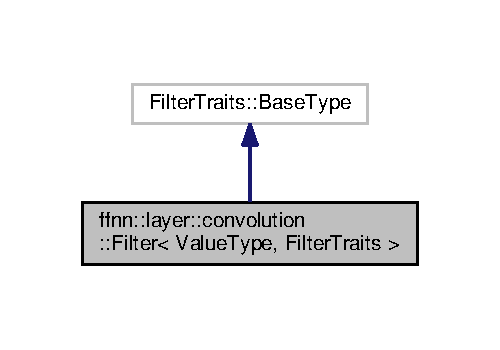
\includegraphics[width=222pt]{structffnn_1_1layer_1_1convolution_1_1_filter__inherit__graph}
\end{center}
\end{figure}


Collaboration diagram for ffnn\-:\-:layer\-:\-:convolution\-:\-:Filter$<$ Value\-Type, Options, Extrinsics $>$\-:\nopagebreak
\begin{figure}[H]
\begin{center}
\leavevmode
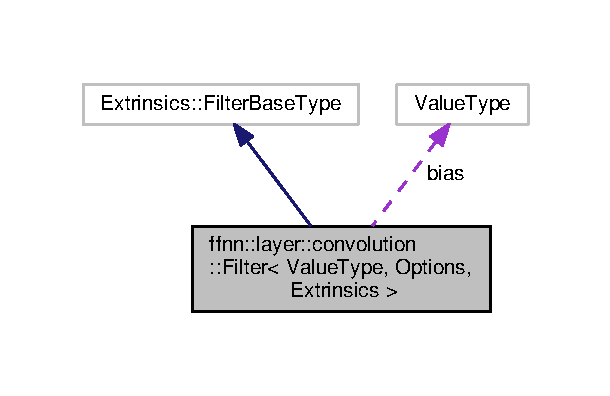
\includegraphics[width=293pt]{structffnn_1_1layer_1_1convolution_1_1_filter__coll__graph}
\end{center}
\end{figure}
\subsection*{Public Types}
\begin{DoxyCompactItemize}
\item 
typedef Extrinsics\-::\-Kernel\-Type \hyperlink{structffnn_1_1layer_1_1convolution_1_1_filter_ad5cce121107613f7bfd80ff7df649b96}{Kernel\-Type}
\begin{DoxyCompactList}\small\item\em \hyperlink{structffnn_1_1layer_1_1convolution_1_1_filter}{Filter} kernel matrix standardization. \end{DoxyCompactList}\end{DoxyCompactItemize}
\subsection*{Public Member Functions}
\begin{DoxyCompactItemize}
\item 
{\footnotesize template$<$bool T = Options\-::has\-\_\-fixed\-\_\-kernel\-\_\-count$>$ }\\\hyperlink{structffnn_1_1layer_1_1convolution_1_1_filter_a92680fc95854201cf47f44ffb91e17e9}{Filter} (typename std\-::enable\-\_\-if$<$ T $>$\-::type $\ast$=nullptr)
\begin{DoxyCompactList}\small\item\em Default constructor. \end{DoxyCompactList}\item 
{\footnotesize template$<$bool T = Options\-::has\-\_\-fixed\-\_\-kernel\-\_\-count$>$ }\\\hyperlink{structffnn_1_1layer_1_1convolution_1_1_filter_ae4efedce4c1e0470bb144b5a1b115465}{Filter} (\hyperlink{namespaceffnn_a63b90a2fd70eb76684eac482a51633e5}{size\-\_\-type} filter\-\_\-count=Eigen\-::\-Dynamic, typename std\-::enable\-\_\-if$<$!T $>$\-::type $\ast$=nullptr)
\item 
{\footnotesize template$<$bool T = Options\-::has\-\_\-fixed\-\_\-kernel\-\_\-count$>$ }\\std\-::enable\-\_\-if$<$ T $>$\-::type \hyperlink{structffnn_1_1layer_1_1convolution_1_1_filter_ac48e60bc36addccf9ac9c10a8afe533d}{set\-Zero} (\hyperlink{namespaceffnn_a63b90a2fd70eb76684eac482a51633e5}{size\-\_\-type} kernel\-\_\-height=Options\-::kernel\-\_\-height, \hyperlink{namespaceffnn_a63b90a2fd70eb76684eac482a51633e5}{size\-\_\-type} kernel\-\_\-width=Options\-::kernel\-\_\-width, \hyperlink{namespaceffnn_a63b90a2fd70eb76684eac482a51633e5}{size\-\_\-type} kernel\-\_\-depth=Options\-::kernel\-\_\-depth, \hyperlink{namespaceffnn_a63b90a2fd70eb76684eac482a51633e5}{size\-\_\-type} kernel\-\_\-count=Options\-::kernel\-\_\-count)
\begin{DoxyCompactList}\small\item\em Sets all \hyperlink{structffnn_1_1layer_1_1convolution_1_1_filter}{Filter} kernels and scalar bias unit to zero. \end{DoxyCompactList}\item 
{\footnotesize template$<$bool T = Options\-::has\-\_\-fixed\-\_\-kernel\-\_\-count$>$ }\\std\-::enable\-\_\-if$<$!T $>$\-::type \hyperlink{structffnn_1_1layer_1_1convolution_1_1_filter_a806c77e5cab9da9dd9761d7bdc2113ea}{set\-Zero} (\hyperlink{namespaceffnn_a63b90a2fd70eb76684eac482a51633e5}{size\-\_\-type} kernel\-\_\-height=Options\-::kernel\-\_\-height, \hyperlink{namespaceffnn_a63b90a2fd70eb76684eac482a51633e5}{size\-\_\-type} kernel\-\_\-width=Options\-::kernel\-\_\-width, \hyperlink{namespaceffnn_a63b90a2fd70eb76684eac482a51633e5}{size\-\_\-type} kernel\-\_\-depth=Options\-::kernel\-\_\-depth, \hyperlink{namespaceffnn_a63b90a2fd70eb76684eac482a51633e5}{size\-\_\-type} kernel\-\_\-count=Options\-::kernel\-\_\-count)
\item 
\hyperlink{structffnn_1_1layer_1_1convolution_1_1_filter}{Filter} \& \hyperlink{structffnn_1_1layer_1_1convolution_1_1_filter_a266f401f904688abe76239cd6563dd3c}{operator$\ast$=} (Value\-Type scale)
\begin{DoxyCompactList}\small\item\em Scales kernels and bias value. \end{DoxyCompactList}\item 
\hyperlink{structffnn_1_1layer_1_1convolution_1_1_filter}{Filter} \& \hyperlink{structffnn_1_1layer_1_1convolution_1_1_filter_ad25eed8e7ffa78ff50fb3318cef81de5}{operator-\/=} (const \hyperlink{structffnn_1_1layer_1_1convolution_1_1_filter}{Filter} \&other)
\begin{DoxyCompactList}\small\item\em In-\/place subtraction between two \hyperlink{structffnn_1_1layer_1_1convolution_1_1_filter}{Filter} objects. \end{DoxyCompactList}\item 
\hyperlink{structffnn_1_1layer_1_1convolution_1_1_filter}{Filter} \& \hyperlink{structffnn_1_1layer_1_1convolution_1_1_filter_a49da4098c5d9a8e400a248a564c84ec1}{operator+=} (const \hyperlink{structffnn_1_1layer_1_1convolution_1_1_filter}{Filter} \&other)
\begin{DoxyCompactList}\small\item\em In-\/place addition between two \hyperlink{structffnn_1_1layer_1_1convolution_1_1_filter}{Filter} objects. \end{DoxyCompactList}\item 
\hyperlink{structffnn_1_1layer_1_1convolution_1_1_filter}{Filter} \& \hyperlink{structffnn_1_1layer_1_1convolution_1_1_filter_aaaa1e310acdc9ab2372109b827d4edaa}{operator$\ast$=} (const \hyperlink{structffnn_1_1layer_1_1convolution_1_1_filter}{Filter} \&other)
\begin{DoxyCompactList}\small\item\em In-\/place coefficient-\/wise multiplication between two \hyperlink{structffnn_1_1layer_1_1convolution_1_1_filter}{Filter} objects. \end{DoxyCompactList}\item 
\hyperlink{structffnn_1_1layer_1_1convolution_1_1_filter}{Filter} \& \hyperlink{structffnn_1_1layer_1_1convolution_1_1_filter_afa3ec94a3919f5e844182e991ef972fc}{operator/=} (const \hyperlink{structffnn_1_1layer_1_1convolution_1_1_filter}{Filter} \&other)
\begin{DoxyCompactList}\small\item\em In-\/place coefficient-\/wise division between two \hyperlink{structffnn_1_1layer_1_1convolution_1_1_filter}{Filter} objects. \end{DoxyCompactList}\item 
\hyperlink{structffnn_1_1layer_1_1convolution_1_1_filter}{Filter} \& \hyperlink{structffnn_1_1layer_1_1convolution_1_1_filter_a67b153ce5dd863e99bd3ba811e557cce}{array} ()
\begin{DoxyCompactList}\small\item\em Returns reference {\ttfamily $\ast$this} \end{DoxyCompactList}\item 
{\footnotesize template$<$class Archive $>$ }\\void \hyperlink{structffnn_1_1layer_1_1convolution_1_1_filter_a339b11d21993373dc8ba26cc14c7d1fc}{save} (Archive \&ar, const unsigned int version) const 
\begin{DoxyCompactList}\small\item\em Save serializer. \end{DoxyCompactList}\item 
{\footnotesize template$<$class Archive , bool T = Options\-::has\-\_\-fixed\-\_\-kernel\-\_\-count$>$ }\\std\-::enable\-\_\-if$<$ T $>$\-::type \hyperlink{structffnn_1_1layer_1_1convolution_1_1_filter_a2526fa5d145e32ca98c600d6114d75da}{load} (Archive \&ar, const unsigned int version)
\begin{DoxyCompactList}\small\item\em Load serializer. \end{DoxyCompactList}\item 
{\footnotesize template$<$class Archive , bool T = Options\-::has\-\_\-fixed\-\_\-kernel\-\_\-count$>$ }\\std\-::enable\-\_\-if$<$!T $>$\-::type \hyperlink{structffnn_1_1layer_1_1convolution_1_1_filter_a53db087b4da6ead13ddefaf0bab7d726}{load} (Archive \&ar, const unsigned int version)
\item 
{\footnotesize template$<$class Archive $>$ }\\void \hyperlink{structffnn_1_1layer_1_1convolution_1_1_filter_a9fd6c03040f1f074eb35092071da0570}{serialize} (Archive \&ar, const unsigned int file\-\_\-version)
\begin{DoxyCompactList}\small\item\em Serializer. \end{DoxyCompactList}\end{DoxyCompactItemize}
\subsection*{Public Attributes}
\begin{DoxyCompactItemize}
\item 
Value\-Type \hyperlink{structffnn_1_1layer_1_1convolution_1_1_filter_a3638f1ebfd8d5d4469392dd7b2470cc3}{bias}
\begin{DoxyCompactList}\small\item\em Bias value. \end{DoxyCompactList}\end{DoxyCompactItemize}


\subsection{Detailed Description}
\subsubsection*{template$<$typename Value\-Type, typename Options = typename filter\-::options$<$$>$, typename Extrinsics = typename filter\-::extrinsics$<$\-Value\-Type, Options$>$$>$struct ffnn\-::layer\-::convolution\-::\-Filter$<$ Value\-Type, Options, Extrinsics $>$}

\hyperlink{structffnn_1_1layer_1_1convolution_1_1_filter}{Filter} parameters to be use with a \hyperlink{classffnn_1_1layer_1_1_convolution}{Convolution} layer. 


\begin{DoxyParams}{Parameters}
{\em Value\-Type} & scalar value type \\
\hline
{\em Options} & filter sizing and data-\/ordering information \\
\hline
\end{DoxyParams}


\subsection{Member Typedef Documentation}
\hypertarget{structffnn_1_1layer_1_1convolution_1_1_filter_ad5cce121107613f7bfd80ff7df649b96}{\index{ffnn\-::layer\-::convolution\-::\-Filter@{ffnn\-::layer\-::convolution\-::\-Filter}!Kernel\-Type@{Kernel\-Type}}
\index{Kernel\-Type@{Kernel\-Type}!ffnn::layer::convolution::Filter@{ffnn\-::layer\-::convolution\-::\-Filter}}
\subsubsection[{Kernel\-Type}]{\setlength{\rightskip}{0pt plus 5cm}template$<$typename Value\-Type , typename Options  = typename filter\-::options$<$$>$, typename Extrinsics  = typename filter\-::extrinsics$<$\-Value\-Type, Options$>$$>$ typedef Extrinsics\-::\-Kernel\-Type {\bf ffnn\-::layer\-::convolution\-::\-Filter}$<$ Value\-Type, Options, Extrinsics $>$\-::{\bf Kernel\-Type}}}\label{structffnn_1_1layer_1_1convolution_1_1_filter_ad5cce121107613f7bfd80ff7df649b96}


\hyperlink{structffnn_1_1layer_1_1convolution_1_1_filter}{Filter} kernel matrix standardization. 



\subsection{Constructor \& Destructor Documentation}
\hypertarget{structffnn_1_1layer_1_1convolution_1_1_filter_a92680fc95854201cf47f44ffb91e17e9}{\index{ffnn\-::layer\-::convolution\-::\-Filter@{ffnn\-::layer\-::convolution\-::\-Filter}!Filter@{Filter}}
\index{Filter@{Filter}!ffnn::layer::convolution::Filter@{ffnn\-::layer\-::convolution\-::\-Filter}}
\subsubsection[{Filter}]{\setlength{\rightskip}{0pt plus 5cm}template$<$typename Value\-Type , typename Options  = typename filter\-::options$<$$>$, typename Extrinsics  = typename filter\-::extrinsics$<$\-Value\-Type, Options$>$$>$ template$<$bool T = Options\-::has\-\_\-fixed\-\_\-kernel\-\_\-count$>$ {\bf ffnn\-::layer\-::convolution\-::\-Filter}$<$ Value\-Type, Options, Extrinsics $>$\-::{\bf Filter} (
\begin{DoxyParamCaption}
\item[{typename std\-::enable\-\_\-if$<$ T $>$\-::type $\ast$}]{ = {\ttfamily nullptr}}
\end{DoxyParamCaption}
)\hspace{0.3cm}{\ttfamily [inline]}}}\label{structffnn_1_1layer_1_1convolution_1_1_filter_a92680fc95854201cf47f44ffb91e17e9}


Default constructor. 

\hypertarget{structffnn_1_1layer_1_1convolution_1_1_filter_ae4efedce4c1e0470bb144b5a1b115465}{\index{ffnn\-::layer\-::convolution\-::\-Filter@{ffnn\-::layer\-::convolution\-::\-Filter}!Filter@{Filter}}
\index{Filter@{Filter}!ffnn::layer::convolution::Filter@{ffnn\-::layer\-::convolution\-::\-Filter}}
\subsubsection[{Filter}]{\setlength{\rightskip}{0pt plus 5cm}template$<$typename Value\-Type , typename Options  = typename filter\-::options$<$$>$, typename Extrinsics  = typename filter\-::extrinsics$<$\-Value\-Type, Options$>$$>$ template$<$bool T = Options\-::has\-\_\-fixed\-\_\-kernel\-\_\-count$>$ {\bf ffnn\-::layer\-::convolution\-::\-Filter}$<$ Value\-Type, Options, Extrinsics $>$\-::{\bf Filter} (
\begin{DoxyParamCaption}
\item[{{\bf size\-\_\-type}}]{filter\-\_\-count = {\ttfamily Eigen\-:\-:Dynamic}, }
\item[{typename std\-::enable\-\_\-if$<$!T $>$\-::type $\ast$}]{ = {\ttfamily nullptr}}
\end{DoxyParamCaption}
)\hspace{0.3cm}{\ttfamily [inline]}}}\label{structffnn_1_1layer_1_1convolution_1_1_filter_ae4efedce4c1e0470bb144b5a1b115465}


\subsection{Member Function Documentation}
\hypertarget{structffnn_1_1layer_1_1convolution_1_1_filter_a67b153ce5dd863e99bd3ba811e557cce}{\index{ffnn\-::layer\-::convolution\-::\-Filter@{ffnn\-::layer\-::convolution\-::\-Filter}!array@{array}}
\index{array@{array}!ffnn::layer::convolution::Filter@{ffnn\-::layer\-::convolution\-::\-Filter}}
\subsubsection[{array}]{\setlength{\rightskip}{0pt plus 5cm}template$<$typename Value\-Type , typename Options  = typename filter\-::options$<$$>$, typename Extrinsics  = typename filter\-::extrinsics$<$\-Value\-Type, Options$>$$>$ {\bf Filter}\& {\bf ffnn\-::layer\-::convolution\-::\-Filter}$<$ Value\-Type, Options, Extrinsics $>$\-::array (
\begin{DoxyParamCaption}
{}
\end{DoxyParamCaption}
)\hspace{0.3cm}{\ttfamily [inline]}}}\label{structffnn_1_1layer_1_1convolution_1_1_filter_a67b153ce5dd863e99bd3ba811e557cce}


Returns reference {\ttfamily $\ast$this} 

\begin{DoxyNote}{Note}
Necessary to fufill {\ttfamily Parameter\-Type} concept 
\end{DoxyNote}


Referenced by ffnn\-::layer\-::convolution\-::\-Filter$<$ Value\-Type, Options, Extrinsics $>$\-::operator$\ast$=(), and ffnn\-::layer\-::convolution\-::\-Filter$<$ Value\-Type, Options, Extrinsics $>$\-::operator/=().

\hypertarget{structffnn_1_1layer_1_1convolution_1_1_filter_a2526fa5d145e32ca98c600d6114d75da}{\index{ffnn\-::layer\-::convolution\-::\-Filter@{ffnn\-::layer\-::convolution\-::\-Filter}!load@{load}}
\index{load@{load}!ffnn::layer::convolution::Filter@{ffnn\-::layer\-::convolution\-::\-Filter}}
\subsubsection[{load}]{\setlength{\rightskip}{0pt plus 5cm}template$<$typename Value\-Type , typename Options  = typename filter\-::options$<$$>$, typename Extrinsics  = typename filter\-::extrinsics$<$\-Value\-Type, Options$>$$>$ template$<$class Archive , bool T = Options\-::has\-\_\-fixed\-\_\-kernel\-\_\-count$>$ std\-::enable\-\_\-if$<$T$>$\-::type {\bf ffnn\-::layer\-::convolution\-::\-Filter}$<$ Value\-Type, Options, Extrinsics $>$\-::load (
\begin{DoxyParamCaption}
\item[{Archive \&}]{ar, }
\item[{const unsigned int}]{version}
\end{DoxyParamCaption}
)\hspace{0.3cm}{\ttfamily [inline]}}}\label{structffnn_1_1layer_1_1convolution_1_1_filter_a2526fa5d145e32ca98c600d6114d75da}


Load serializer. 


\begin{DoxyParams}{Parameters}
{\em ar} & input archive \\
\hline
{\em version} & archive versioning information \\
\hline
\end{DoxyParams}
\begin{DoxyNote}{Note}
Statically sized version 
\end{DoxyNote}
\hypertarget{structffnn_1_1layer_1_1convolution_1_1_filter_a53db087b4da6ead13ddefaf0bab7d726}{\index{ffnn\-::layer\-::convolution\-::\-Filter@{ffnn\-::layer\-::convolution\-::\-Filter}!load@{load}}
\index{load@{load}!ffnn::layer::convolution::Filter@{ffnn\-::layer\-::convolution\-::\-Filter}}
\subsubsection[{load}]{\setlength{\rightskip}{0pt plus 5cm}template$<$typename Value\-Type , typename Options  = typename filter\-::options$<$$>$, typename Extrinsics  = typename filter\-::extrinsics$<$\-Value\-Type, Options$>$$>$ template$<$class Archive , bool T = Options\-::has\-\_\-fixed\-\_\-kernel\-\_\-count$>$ std\-::enable\-\_\-if$<$!T$>$\-::type {\bf ffnn\-::layer\-::convolution\-::\-Filter}$<$ Value\-Type, Options, Extrinsics $>$\-::load (
\begin{DoxyParamCaption}
\item[{Archive \&}]{ar, }
\item[{const unsigned int}]{version}
\end{DoxyParamCaption}
)\hspace{0.3cm}{\ttfamily [inline]}}}\label{structffnn_1_1layer_1_1convolution_1_1_filter_a53db087b4da6ead13ddefaf0bab7d726}
\hypertarget{structffnn_1_1layer_1_1convolution_1_1_filter_a266f401f904688abe76239cd6563dd3c}{\index{ffnn\-::layer\-::convolution\-::\-Filter@{ffnn\-::layer\-::convolution\-::\-Filter}!operator$\ast$=@{operator$\ast$=}}
\index{operator$\ast$=@{operator$\ast$=}!ffnn::layer::convolution::Filter@{ffnn\-::layer\-::convolution\-::\-Filter}}
\subsubsection[{operator$\ast$=}]{\setlength{\rightskip}{0pt plus 5cm}template$<$typename Value\-Type , typename Options  = typename filter\-::options$<$$>$, typename Extrinsics  = typename filter\-::extrinsics$<$\-Value\-Type, Options$>$$>$ {\bf Filter}\& {\bf ffnn\-::layer\-::convolution\-::\-Filter}$<$ Value\-Type, Options, Extrinsics $>$\-::operator$\ast$= (
\begin{DoxyParamCaption}
\item[{Value\-Type}]{scale}
\end{DoxyParamCaption}
)\hspace{0.3cm}{\ttfamily [inline]}}}\label{structffnn_1_1layer_1_1convolution_1_1_filter_a266f401f904688abe76239cd6563dd3c}


Scales kernels and bias value. 


\begin{DoxyParams}{Parameters}
{\em scale} & scalar value \\
\hline
\end{DoxyParams}
\begin{DoxyReturn}{Returns}
$\ast$this 
\end{DoxyReturn}
\hypertarget{structffnn_1_1layer_1_1convolution_1_1_filter_aaaa1e310acdc9ab2372109b827d4edaa}{\index{ffnn\-::layer\-::convolution\-::\-Filter@{ffnn\-::layer\-::convolution\-::\-Filter}!operator$\ast$=@{operator$\ast$=}}
\index{operator$\ast$=@{operator$\ast$=}!ffnn::layer::convolution::Filter@{ffnn\-::layer\-::convolution\-::\-Filter}}
\subsubsection[{operator$\ast$=}]{\setlength{\rightskip}{0pt plus 5cm}template$<$typename Value\-Type , typename Options  = typename filter\-::options$<$$>$, typename Extrinsics  = typename filter\-::extrinsics$<$\-Value\-Type, Options$>$$>$ {\bf Filter}\& {\bf ffnn\-::layer\-::convolution\-::\-Filter}$<$ Value\-Type, Options, Extrinsics $>$\-::operator$\ast$= (
\begin{DoxyParamCaption}
\item[{const {\bf Filter}$<$ Value\-Type, Options, Extrinsics $>$ \&}]{other}
\end{DoxyParamCaption}
)\hspace{0.3cm}{\ttfamily [inline]}}}\label{structffnn_1_1layer_1_1convolution_1_1_filter_aaaa1e310acdc9ab2372109b827d4edaa}


In-\/place coefficient-\/wise multiplication between two \hyperlink{structffnn_1_1layer_1_1convolution_1_1_filter}{Filter} objects. 


\begin{DoxyParams}{Parameters}
{\em other} & \hyperlink{structffnn_1_1layer_1_1convolution_1_1_filter}{Filter} object \\
\hline
\end{DoxyParams}
\begin{DoxyReturn}{Returns}
$\ast$this 
\end{DoxyReturn}


Here is the call graph for this function\-:\nopagebreak
\begin{figure}[H]
\begin{center}
\leavevmode
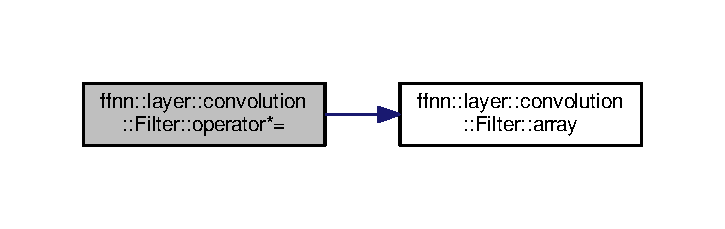
\includegraphics[width=348pt]{structffnn_1_1layer_1_1convolution_1_1_filter_aaaa1e310acdc9ab2372109b827d4edaa_cgraph}
\end{center}
\end{figure}


\hypertarget{structffnn_1_1layer_1_1convolution_1_1_filter_a49da4098c5d9a8e400a248a564c84ec1}{\index{ffnn\-::layer\-::convolution\-::\-Filter@{ffnn\-::layer\-::convolution\-::\-Filter}!operator+=@{operator+=}}
\index{operator+=@{operator+=}!ffnn::layer::convolution::Filter@{ffnn\-::layer\-::convolution\-::\-Filter}}
\subsubsection[{operator+=}]{\setlength{\rightskip}{0pt plus 5cm}template$<$typename Value\-Type , typename Options  = typename filter\-::options$<$$>$, typename Extrinsics  = typename filter\-::extrinsics$<$\-Value\-Type, Options$>$$>$ {\bf Filter}\& {\bf ffnn\-::layer\-::convolution\-::\-Filter}$<$ Value\-Type, Options, Extrinsics $>$\-::operator+= (
\begin{DoxyParamCaption}
\item[{const {\bf Filter}$<$ Value\-Type, Options, Extrinsics $>$ \&}]{other}
\end{DoxyParamCaption}
)\hspace{0.3cm}{\ttfamily [inline]}}}\label{structffnn_1_1layer_1_1convolution_1_1_filter_a49da4098c5d9a8e400a248a564c84ec1}


In-\/place addition between two \hyperlink{structffnn_1_1layer_1_1convolution_1_1_filter}{Filter} objects. 


\begin{DoxyParams}{Parameters}
{\em other} & \hyperlink{structffnn_1_1layer_1_1convolution_1_1_filter}{Filter} object \\
\hline
\end{DoxyParams}
\begin{DoxyReturn}{Returns}
$\ast$this 
\end{DoxyReturn}
\hypertarget{structffnn_1_1layer_1_1convolution_1_1_filter_ad25eed8e7ffa78ff50fb3318cef81de5}{\index{ffnn\-::layer\-::convolution\-::\-Filter@{ffnn\-::layer\-::convolution\-::\-Filter}!operator-\/=@{operator-\/=}}
\index{operator-\/=@{operator-\/=}!ffnn::layer::convolution::Filter@{ffnn\-::layer\-::convolution\-::\-Filter}}
\subsubsection[{operator-\/=}]{\setlength{\rightskip}{0pt plus 5cm}template$<$typename Value\-Type , typename Options  = typename filter\-::options$<$$>$, typename Extrinsics  = typename filter\-::extrinsics$<$\-Value\-Type, Options$>$$>$ {\bf Filter}\& {\bf ffnn\-::layer\-::convolution\-::\-Filter}$<$ Value\-Type, Options, Extrinsics $>$\-::operator-\/= (
\begin{DoxyParamCaption}
\item[{const {\bf Filter}$<$ Value\-Type, Options, Extrinsics $>$ \&}]{other}
\end{DoxyParamCaption}
)\hspace{0.3cm}{\ttfamily [inline]}}}\label{structffnn_1_1layer_1_1convolution_1_1_filter_ad25eed8e7ffa78ff50fb3318cef81de5}


In-\/place subtraction between two \hyperlink{structffnn_1_1layer_1_1convolution_1_1_filter}{Filter} objects. 


\begin{DoxyParams}{Parameters}
{\em other} & \hyperlink{structffnn_1_1layer_1_1convolution_1_1_filter}{Filter} object \\
\hline
\end{DoxyParams}
\begin{DoxyReturn}{Returns}
$\ast$this 
\end{DoxyReturn}
\hypertarget{structffnn_1_1layer_1_1convolution_1_1_filter_afa3ec94a3919f5e844182e991ef972fc}{\index{ffnn\-::layer\-::convolution\-::\-Filter@{ffnn\-::layer\-::convolution\-::\-Filter}!operator/=@{operator/=}}
\index{operator/=@{operator/=}!ffnn::layer::convolution::Filter@{ffnn\-::layer\-::convolution\-::\-Filter}}
\subsubsection[{operator/=}]{\setlength{\rightskip}{0pt plus 5cm}template$<$typename Value\-Type , typename Options  = typename filter\-::options$<$$>$, typename Extrinsics  = typename filter\-::extrinsics$<$\-Value\-Type, Options$>$$>$ {\bf Filter}\& {\bf ffnn\-::layer\-::convolution\-::\-Filter}$<$ Value\-Type, Options, Extrinsics $>$\-::operator/= (
\begin{DoxyParamCaption}
\item[{const {\bf Filter}$<$ Value\-Type, Options, Extrinsics $>$ \&}]{other}
\end{DoxyParamCaption}
)\hspace{0.3cm}{\ttfamily [inline]}}}\label{structffnn_1_1layer_1_1convolution_1_1_filter_afa3ec94a3919f5e844182e991ef972fc}


In-\/place coefficient-\/wise division between two \hyperlink{structffnn_1_1layer_1_1convolution_1_1_filter}{Filter} objects. 


\begin{DoxyParams}{Parameters}
{\em other} & \hyperlink{structffnn_1_1layer_1_1convolution_1_1_filter}{Filter} object \\
\hline
\end{DoxyParams}
\begin{DoxyReturn}{Returns}
$\ast$this 
\end{DoxyReturn}


Here is the call graph for this function\-:\nopagebreak
\begin{figure}[H]
\begin{center}
\leavevmode
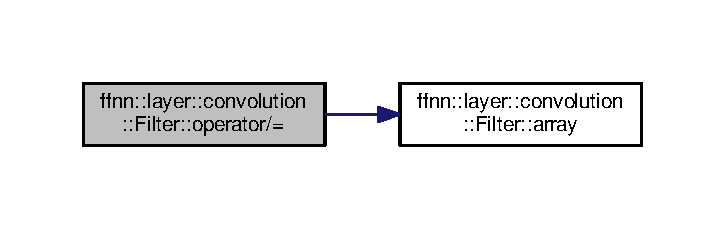
\includegraphics[width=348pt]{structffnn_1_1layer_1_1convolution_1_1_filter_afa3ec94a3919f5e844182e991ef972fc_cgraph}
\end{center}
\end{figure}


\hypertarget{structffnn_1_1layer_1_1convolution_1_1_filter_a339b11d21993373dc8ba26cc14c7d1fc}{\index{ffnn\-::layer\-::convolution\-::\-Filter@{ffnn\-::layer\-::convolution\-::\-Filter}!save@{save}}
\index{save@{save}!ffnn::layer::convolution::Filter@{ffnn\-::layer\-::convolution\-::\-Filter}}
\subsubsection[{save}]{\setlength{\rightskip}{0pt plus 5cm}template$<$typename Value\-Type , typename Options  = typename filter\-::options$<$$>$, typename Extrinsics  = typename filter\-::extrinsics$<$\-Value\-Type, Options$>$$>$ template$<$class Archive $>$ void {\bf ffnn\-::layer\-::convolution\-::\-Filter}$<$ Value\-Type, Options, Extrinsics $>$\-::save (
\begin{DoxyParamCaption}
\item[{Archive \&}]{ar, }
\item[{const unsigned int}]{version}
\end{DoxyParamCaption}
) const\hspace{0.3cm}{\ttfamily [inline]}}}\label{structffnn_1_1layer_1_1convolution_1_1_filter_a339b11d21993373dc8ba26cc14c7d1fc}


Save serializer. 


\begin{DoxyParams}{Parameters}
{\em ar} & output archive \\
\hline
{\em version} & archive versioning information \\
\hline
\end{DoxyParams}
\hypertarget{structffnn_1_1layer_1_1convolution_1_1_filter_a9fd6c03040f1f074eb35092071da0570}{\index{ffnn\-::layer\-::convolution\-::\-Filter@{ffnn\-::layer\-::convolution\-::\-Filter}!serialize@{serialize}}
\index{serialize@{serialize}!ffnn::layer::convolution::Filter@{ffnn\-::layer\-::convolution\-::\-Filter}}
\subsubsection[{serialize}]{\setlength{\rightskip}{0pt plus 5cm}template$<$typename Value\-Type , typename Options  = typename filter\-::options$<$$>$, typename Extrinsics  = typename filter\-::extrinsics$<$\-Value\-Type, Options$>$$>$ template$<$class Archive $>$ void {\bf ffnn\-::layer\-::convolution\-::\-Filter}$<$ Value\-Type, Options, Extrinsics $>$\-::serialize (
\begin{DoxyParamCaption}
\item[{Archive \&}]{ar, }
\item[{const unsigned int}]{file\-\_\-version}
\end{DoxyParamCaption}
)\hspace{0.3cm}{\ttfamily [inline]}}}\label{structffnn_1_1layer_1_1convolution_1_1_filter_a9fd6c03040f1f074eb35092071da0570}


Serializer. 


\begin{DoxyParams}{Parameters}
{\em ar} & input/output archive \\
\hline
{\em version} & archive versioning information \\
\hline
\end{DoxyParams}
\hypertarget{structffnn_1_1layer_1_1convolution_1_1_filter_ac48e60bc36addccf9ac9c10a8afe533d}{\index{ffnn\-::layer\-::convolution\-::\-Filter@{ffnn\-::layer\-::convolution\-::\-Filter}!set\-Zero@{set\-Zero}}
\index{set\-Zero@{set\-Zero}!ffnn::layer::convolution::Filter@{ffnn\-::layer\-::convolution\-::\-Filter}}
\subsubsection[{set\-Zero}]{\setlength{\rightskip}{0pt plus 5cm}template$<$typename Value\-Type , typename Options  = typename filter\-::options$<$$>$, typename Extrinsics  = typename filter\-::extrinsics$<$\-Value\-Type, Options$>$$>$ template$<$bool T = Options\-::has\-\_\-fixed\-\_\-kernel\-\_\-count$>$ std\-::enable\-\_\-if$<$T$>$\-::type {\bf ffnn\-::layer\-::convolution\-::\-Filter}$<$ Value\-Type, Options, Extrinsics $>$\-::set\-Zero (
\begin{DoxyParamCaption}
\item[{{\bf size\-\_\-type}}]{kernel\-\_\-height = {\ttfamily Options\-:\-:kernel\-\_\-height}, }
\item[{{\bf size\-\_\-type}}]{kernel\-\_\-width = {\ttfamily Options\-:\-:kernel\-\_\-width}, }
\item[{{\bf size\-\_\-type}}]{kernel\-\_\-depth = {\ttfamily Options\-:\-:kernel\-\_\-depth}, }
\item[{{\bf size\-\_\-type}}]{kernel\-\_\-count = {\ttfamily Options\-:\-:kernel\-\_\-count}}
\end{DoxyParamCaption}
)\hspace{0.3cm}{\ttfamily [inline]}}}\label{structffnn_1_1layer_1_1convolution_1_1_filter_ac48e60bc36addccf9ac9c10a8afe533d}


Sets all \hyperlink{structffnn_1_1layer_1_1convolution_1_1_filter}{Filter} kernels and scalar bias unit to zero. 


\begin{DoxyParams}{Parameters}
{\em kernel\-\_\-height} & height of filter kernel \\
\hline
{\em kernel\-\_\-width} & width of filter kernel \\
\hline
{\em kernel\-\_\-depth} & depth of filter kernel \\
\hline
{\em kernel\-\_\-count} & number of kernels \\
\hline
\end{DoxyParams}
\hypertarget{structffnn_1_1layer_1_1convolution_1_1_filter_a806c77e5cab9da9dd9761d7bdc2113ea}{\index{ffnn\-::layer\-::convolution\-::\-Filter@{ffnn\-::layer\-::convolution\-::\-Filter}!set\-Zero@{set\-Zero}}
\index{set\-Zero@{set\-Zero}!ffnn::layer::convolution::Filter@{ffnn\-::layer\-::convolution\-::\-Filter}}
\subsubsection[{set\-Zero}]{\setlength{\rightskip}{0pt plus 5cm}template$<$typename Value\-Type , typename Options  = typename filter\-::options$<$$>$, typename Extrinsics  = typename filter\-::extrinsics$<$\-Value\-Type, Options$>$$>$ template$<$bool T = Options\-::has\-\_\-fixed\-\_\-kernel\-\_\-count$>$ std\-::enable\-\_\-if$<$!T$>$\-::type {\bf ffnn\-::layer\-::convolution\-::\-Filter}$<$ Value\-Type, Options, Extrinsics $>$\-::set\-Zero (
\begin{DoxyParamCaption}
\item[{{\bf size\-\_\-type}}]{kernel\-\_\-height = {\ttfamily Options\-:\-:kernel\-\_\-height}, }
\item[{{\bf size\-\_\-type}}]{kernel\-\_\-width = {\ttfamily Options\-:\-:kernel\-\_\-width}, }
\item[{{\bf size\-\_\-type}}]{kernel\-\_\-depth = {\ttfamily Options\-:\-:kernel\-\_\-depth}, }
\item[{{\bf size\-\_\-type}}]{kernel\-\_\-count = {\ttfamily Options\-:\-:kernel\-\_\-count}}
\end{DoxyParamCaption}
)\hspace{0.3cm}{\ttfamily [inline]}}}\label{structffnn_1_1layer_1_1convolution_1_1_filter_a806c77e5cab9da9dd9761d7bdc2113ea}


\subsection{Member Data Documentation}
\hypertarget{structffnn_1_1layer_1_1convolution_1_1_filter_a3638f1ebfd8d5d4469392dd7b2470cc3}{\index{ffnn\-::layer\-::convolution\-::\-Filter@{ffnn\-::layer\-::convolution\-::\-Filter}!bias@{bias}}
\index{bias@{bias}!ffnn::layer::convolution::Filter@{ffnn\-::layer\-::convolution\-::\-Filter}}
\subsubsection[{bias}]{\setlength{\rightskip}{0pt plus 5cm}template$<$typename Value\-Type , typename Options  = typename filter\-::options$<$$>$, typename Extrinsics  = typename filter\-::extrinsics$<$\-Value\-Type, Options$>$$>$ Value\-Type {\bf ffnn\-::layer\-::convolution\-::\-Filter}$<$ Value\-Type, Options, Extrinsics $>$\-::bias}}\label{structffnn_1_1layer_1_1convolution_1_1_filter_a3638f1ebfd8d5d4469392dd7b2470cc3}


Bias value. 



Referenced by ffnn\-::layer\-::convolution\-::\-Filter$<$ Value\-Type, Options, Extrinsics $>$\-::load(), ffnn\-::layer\-::convolution\-::\-Filter$<$ Value\-Type, Options, Extrinsics $>$\-::operator$\ast$=(), ffnn\-::layer\-::convolution\-::\-Filter$<$ Value\-Type, Options, Extrinsics $>$\-::operator+=(), ffnn\-::layer\-::convolution\-::\-Filter$<$ Value\-Type, Options, Extrinsics $>$\-::operator-\/=(), ffnn\-::layer\-::convolution\-::\-Filter$<$ Value\-Type, Options, Extrinsics $>$\-::operator/=(), ffnn\-::layer\-::convolution\-::\-Filter$<$ Value\-Type, Options, Extrinsics $>$\-::save(), and ffnn\-::layer\-::convolution\-::\-Filter$<$ Value\-Type, Options, Extrinsics $>$\-::set\-Zero().



The documentation for this struct was generated from the following file\-:\begin{DoxyCompactItemize}
\item 
/home/briancairl/packages/src/ffnn-\/cpp/ffnn/include/ffnn/layer/convolution/\hyperlink{filter_8h}{filter.\-h}\end{DoxyCompactItemize}

\hypertarget{classffnn_1_1layer_1_1_fully_connected}{\section{ffnn\-:\-:layer\-:\-:Fully\-Connected$<$ Value\-Type, Inputs\-At\-Compile\-Time, Outputs\-At\-Compile\-Time, \-\_\-\-Hidden\-Layer\-Shape $>$ Class Template Reference}
\label{classffnn_1_1layer_1_1_fully_connected}\index{ffnn\-::layer\-::\-Fully\-Connected$<$ Value\-Type, Inputs\-At\-Compile\-Time, Outputs\-At\-Compile\-Time, \-\_\-\-Hidden\-Layer\-Shape $>$@{ffnn\-::layer\-::\-Fully\-Connected$<$ Value\-Type, Inputs\-At\-Compile\-Time, Outputs\-At\-Compile\-Time, \-\_\-\-Hidden\-Layer\-Shape $>$}}
}


A fully-\/connected layer.  




{\ttfamily \#include \char`\"{}fully\-\_\-connected.\-h\char`\"{}}



Inheritance diagram for ffnn\-:\-:layer\-:\-:Fully\-Connected$<$ Value\-Type, Inputs\-At\-Compile\-Time, Outputs\-At\-Compile\-Time, \-\_\-\-Hidden\-Layer\-Shape $>$\-:\nopagebreak
\begin{figure}[H]
\begin{center}
\leavevmode
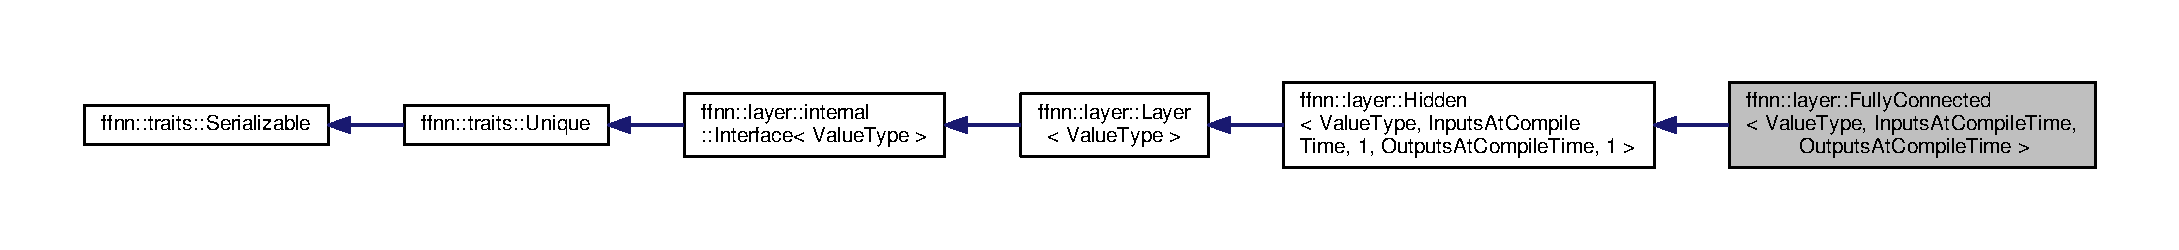
\includegraphics[width=302pt]{classffnn_1_1layer_1_1_fully_connected__inherit__graph}
\end{center}
\end{figure}


Collaboration diagram for ffnn\-:\-:layer\-:\-:Fully\-Connected$<$ Value\-Type, Inputs\-At\-Compile\-Time, Outputs\-At\-Compile\-Time, \-\_\-\-Hidden\-Layer\-Shape $>$\-:\nopagebreak
\begin{figure}[H]
\begin{center}
\leavevmode
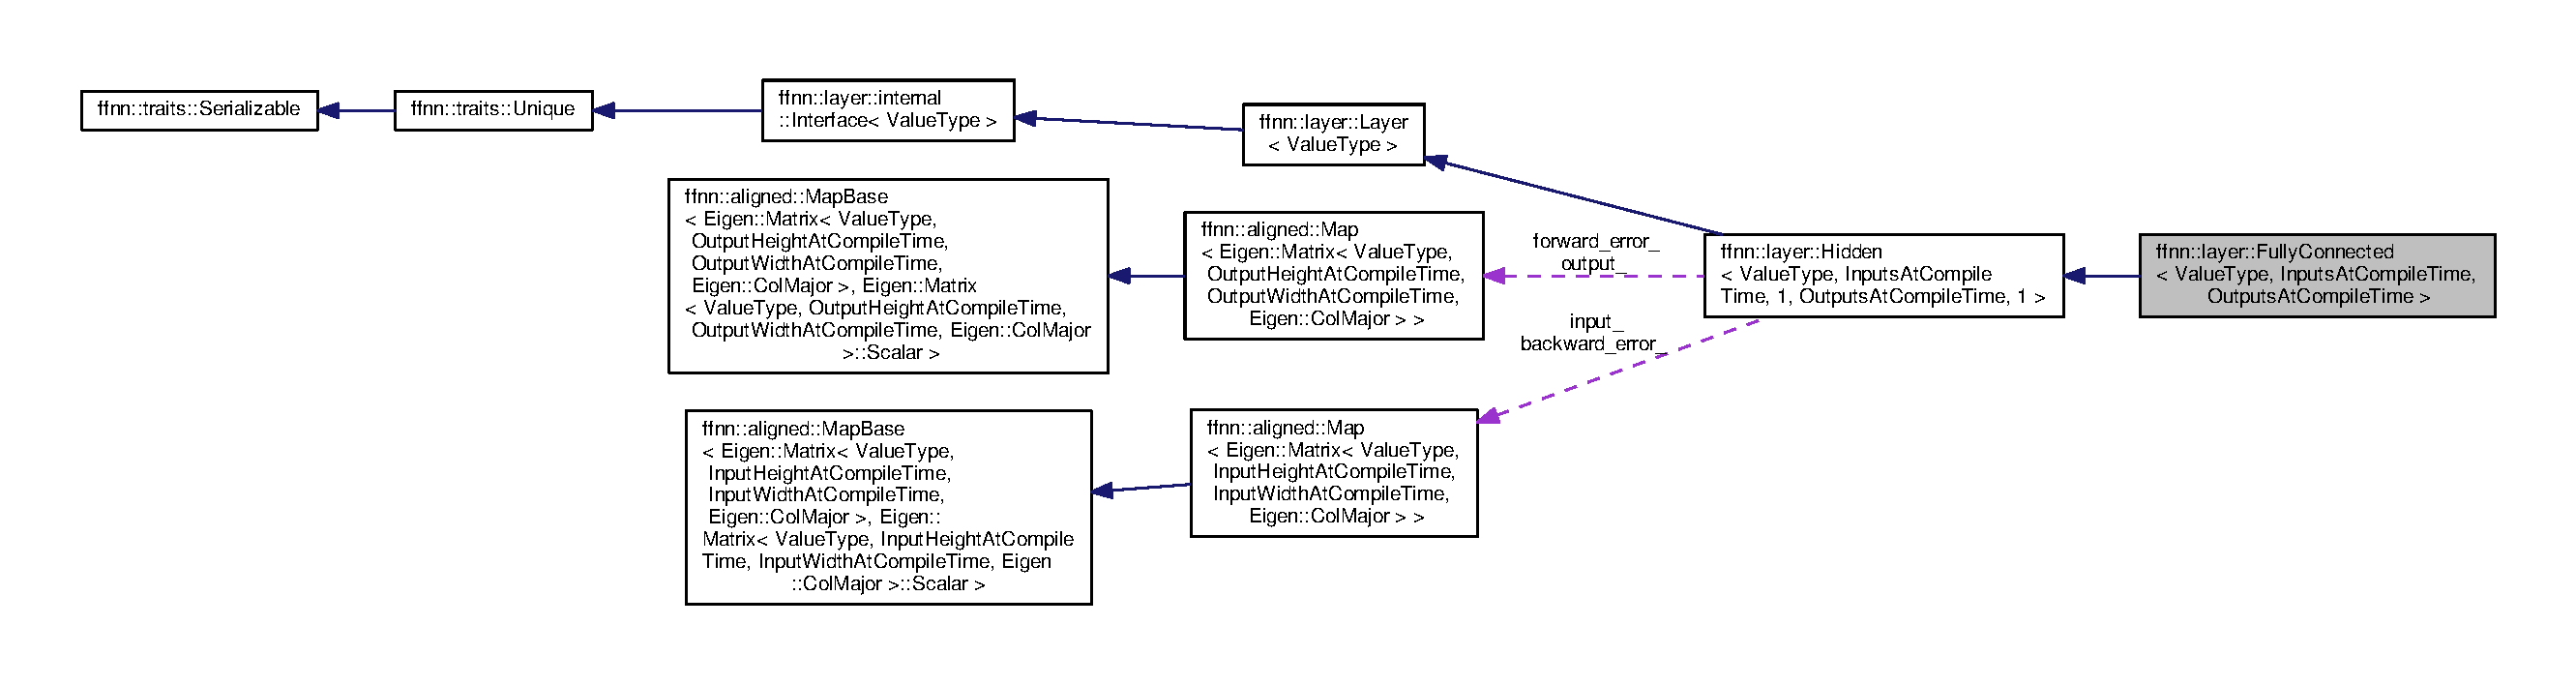
\includegraphics[width=350pt]{classffnn_1_1layer_1_1_fully_connected__coll__graph}
\end{center}
\end{figure}
\subsection*{Public Types}
\begin{DoxyCompactItemize}
\item 
using \hyperlink{classffnn_1_1layer_1_1_fully_connected_ad49d4e88823497be658d01c44eeef3f2}{Base} = \hyperlink{classffnn_1_1layer_1_1_hidden}{Hidden}$<$ Value\-Type, \-\_\-\-Hidden\-Layer\-Shape $>$
\begin{DoxyCompactList}\small\item\em Base type alias. \end{DoxyCompactList}\item 
using \hyperlink{classffnn_1_1layer_1_1_fully_connected_ac41b1867a1a4e8c9c9eaa892db2ab805}{Self} = \hyperlink{classffnn_1_1layer_1_1_fully_connected}{Fully\-Connected}$<$ Value\-Type, Inputs\-At\-Compile\-Time, Outputs\-At\-Compile\-Time $>$
\begin{DoxyCompactList}\small\item\em Self type alias. \end{DoxyCompactList}\item 
typedef \hyperlink{classffnn_1_1layer_1_1_layer_a3d482813f86f1ec69554b4592c478c32}{Base\-::\-Scalar\-Type} \hyperlink{classffnn_1_1layer_1_1_fully_connected_aa5e1875ec3ea63c90655419e7dd32a55}{Scalar\-Type}
\begin{DoxyCompactList}\small\item\em Scalar type standardization. \end{DoxyCompactList}\item 
typedef Base\-::\-Size\-Type \hyperlink{classffnn_1_1layer_1_1_fully_connected_a2924c85b3cc3e79db3f271cd22cac32c}{Size\-Type}
\begin{DoxyCompactList}\small\item\em Size type standardization. \end{DoxyCompactList}\item 
typedef Base\-::\-Offset\-Type \hyperlink{classffnn_1_1layer_1_1_fully_connected_a0f5ae1a0bd038f404410ce2af1054833}{Offset\-Type}
\begin{DoxyCompactList}\small\item\em Offset type standardization. \end{DoxyCompactList}\item 
typedef \hyperlink{classffnn_1_1layer_1_1_hidden_a567e902299b3355501393cf6c7b27c38}{Base\-::\-Shape\-Type} \hyperlink{classffnn_1_1layer_1_1_fully_connected_a938c80efb16baa531fb424626f339333}{Shape\-Type}
\begin{DoxyCompactList}\small\item\em Dimension type standardization. \end{DoxyCompactList}\item 
typedef \hyperlink{classffnn_1_1layer_1_1_hidden_abd5a3b5c55984948f903fe88759efaf4}{Base\-::\-Input\-Block\-Type} \hyperlink{classffnn_1_1layer_1_1_fully_connected_a1360eaafde26c8b36ddb6fe4095b6119}{Input\-Block\-Type}
\begin{DoxyCompactList}\small\item\em Matrix type standardization. \end{DoxyCompactList}\item 
typedef \hyperlink{classffnn_1_1layer_1_1_hidden_a9fd326932b57e1d86d86bdb168822727}{Base\-::\-Output\-Block\-Type} \hyperlink{classffnn_1_1layer_1_1_fully_connected_a23903ba58825efec173f318ffdc3b998}{Output\-Block\-Type}
\begin{DoxyCompactList}\small\item\em Matrix type standardization. \end{DoxyCompactList}\item 
typedef \hyperlink{classffnn_1_1layer_1_1_hidden_a9fd326932b57e1d86d86bdb168822727}{Base\-::\-Output\-Block\-Type} \hyperlink{classffnn_1_1layer_1_1_fully_connected_afd08719c4360bd1447d1108396b07e57}{Bias\-Vector\-Type}
\begin{DoxyCompactList}\small\item\em Bia vector type standardization. \end{DoxyCompactList}\item 
typedef Eigen\-::\-Matrix\\*
$<$ Value\-Type, \\*
Outputs\-At\-Compile\-Time, \\*
Inputs\-At\-Compile\-Time, \\*
Eigen\-::\-Col\-Major $>$ \hyperlink{classffnn_1_1layer_1_1_fully_connected_aef17d91a349bf83f5e5a20462ebb3c81}{Weight\-Matrix\-Type}
\begin{DoxyCompactList}\small\item\em Input-\/output weight matrix. \end{DoxyCompactList}\item 
typedef \hyperlink{classffnn_1_1optimizer_1_1_optimizer}{optimizer\-::\-Optimizer}\\*
$<$ \hyperlink{classffnn_1_1layer_1_1_fully_connected_ac41b1867a1a4e8c9c9eaa892db2ab805}{Self} $>$ \hyperlink{classffnn_1_1layer_1_1_fully_connected_abae398e6ffb06d183654e5ff11857a03}{Optimizer}
\begin{DoxyCompactList}\small\item\em \hyperlink{classffnn_1_1layer_1_1_layer}{Layer} optimization type standardization. \end{DoxyCompactList}\end{DoxyCompactItemize}
\subsection*{Public Member Functions}
\begin{DoxyCompactItemize}
\item 
\hyperlink{classffnn_1_1layer_1_1_fully_connected_a3d846cacf7bcbab5dd193b30a16011f2}{Fully\-Connected} (\hyperlink{classffnn_1_1layer_1_1_fully_connected_a2924c85b3cc3e79db3f271cd22cac32c}{Size\-Type} output\-\_\-size=Outputs\-At\-Compile\-Time)
\begin{DoxyCompactList}\small\item\em Setup constructor. \end{DoxyCompactList}\item 
virtual \hyperlink{classffnn_1_1layer_1_1_fully_connected_ad95d27ee5f609c3a9e5c734aed55b935}{$\sim$\-Fully\-Connected} ()
\item 
bool \hyperlink{classffnn_1_1layer_1_1_fully_connected_a55089e2810d6848950da5ca33000da8a}{initialize} ()
\begin{DoxyCompactList}\small\item\em Initialize the layer. \end{DoxyCompactList}\item 
{\footnotesize template$<$typename Weight\-Distribution , typename Bias\-Distribution $>$ }\\bool \hyperlink{classffnn_1_1layer_1_1_fully_connected_a044ad3ef520054c9e94cc80d5096ce47}{initialize} (const Weight\-Distribution \&wd, const Bias\-Distribution \&bd)
\begin{DoxyCompactList}\small\item\em Initialize layer weights and biases according to particular distributions. \end{DoxyCompactList}\item 
bool \hyperlink{classffnn_1_1layer_1_1_fully_connected_a350e7910bd416f67d30113425ea74f59}{forward} ()
\begin{DoxyCompactList}\small\item\em Performs forward value propagation. \end{DoxyCompactList}\item 
bool \hyperlink{classffnn_1_1layer_1_1_fully_connected_ab4a63eb87bd3f2288258b341fcfd165f}{backward} ()
\begin{DoxyCompactList}\small\item\em Performs backward error propagation. \end{DoxyCompactList}\item 
bool \hyperlink{classffnn_1_1layer_1_1_fully_connected_a7dd4dbe010c3d290c131b21b35f6301e}{update} ()
\begin{DoxyCompactList}\small\item\em Applies accumulated layer weight updates computed during optimization. \end{DoxyCompactList}\item 
void \hyperlink{classffnn_1_1layer_1_1_fully_connected_aaeb55e214173a632b297d3ddac76fc24}{reset} ()
\begin{DoxyCompactList}\small\item\em Reset weights and biases. \end{DoxyCompactList}\item 
void \hyperlink{classffnn_1_1layer_1_1_fully_connected_ae57e6eedc1808825635a1c04aa018992}{set\-Optimizer} (typename \hyperlink{classffnn_1_1optimizer_1_1_optimizer_ac03e7181934bf0c12a97fc67a60484ab}{Optimizer\-::\-Ptr} opt)
\begin{DoxyCompactList}\small\item\em Sets an optimizer used update network weights during back-\/propagation. \end{DoxyCompactList}\item 
const \hyperlink{classffnn_1_1layer_1_1_fully_connected_aef17d91a349bf83f5e5a20462ebb3c81}{Weight\-Matrix\-Type} \& \hyperlink{classffnn_1_1layer_1_1_fully_connected_a96e00e6f6fec19f22a8830e5342bc7ef}{get\-Weights} () const 
\begin{DoxyCompactList}\small\item\em Exposes internal connection weights. \end{DoxyCompactList}\item 
const \hyperlink{classffnn_1_1layer_1_1_fully_connected_afd08719c4360bd1447d1108396b07e57}{Bias\-Vector\-Type} \& \hyperlink{classffnn_1_1layer_1_1_fully_connected_af7492d5d678fd45466d7768ab187a41e}{get\-Biases} () const 
\begin{DoxyCompactList}\small\item\em Exposes internal biasing weights. \end{DoxyCompactList}\item 
\hyperlink{classffnn_1_1layer_1_1_fully_connected_af771581b96123f77fffd9d344c700dc4}{E\-I\-G\-E\-N\-\_\-\-M\-A\-K\-E\-\_\-\-A\-L\-I\-G\-N\-E\-D\-\_\-\-O\-P\-E\-R\-A\-T\-O\-R\-\_\-\-N\-E\-W\-\_\-\-I\-F} (\hyperlink{structffnn_1_1internal_1_1traits_1_1is__alignable__128}{ffnn\-::internal\-::traits\-::is\-\_\-alignable\-\_\-128}$<$ \hyperlink{classffnn_1_1layer_1_1_fully_connected_aef17d91a349bf83f5e5a20462ebb3c81}{Weight\-Matrix\-Type} $>$\-::value$\vert$$\vert$\hyperlink{structffnn_1_1internal_1_1traits_1_1is__alignable__128}{ffnn\-::internal\-::traits\-::is\-\_\-alignable\-\_\-128}$<$ \hyperlink{classffnn_1_1layer_1_1_fully_connected_afd08719c4360bd1447d1108396b07e57}{Bias\-Vector\-Type} $>$\-::value)
\end{DoxyCompactItemize}
\subsection*{Protected Member Functions}
\begin{DoxyCompactItemize}
\item 
void \hyperlink{classffnn_1_1layer_1_1_fully_connected_a7c79eb99c638b61f76ea34b725c0aeef}{save} (\hyperlink{classffnn_1_1internal_1_1_serializable_acf5baead716eb277337a4437e88a5743}{Output\-Archive} \&ar, \hyperlink{classffnn_1_1internal_1_1_serializable_a32fe7d82b0caf9fe8b6fb7c312a26028}{Version\-Type} version) const 
\begin{DoxyCompactList}\small\item\em Save serialize. \end{DoxyCompactList}\item 
void \hyperlink{classffnn_1_1layer_1_1_fully_connected_a1ff2a601cdf315ce46a2812b4e6fe354}{load} (\hyperlink{classffnn_1_1internal_1_1_serializable_aadc27d79d606f35a82dd88bad33fa6d2}{Input\-Archive} \&ar, \hyperlink{classffnn_1_1internal_1_1_serializable_a32fe7d82b0caf9fe8b6fb7c312a26028}{Version\-Type} version)
\begin{DoxyCompactList}\small\item\em Load serialize. \end{DoxyCompactList}\end{DoxyCompactItemize}
\subsection*{Additional Inherited Members}


\subsection{Detailed Description}
\subsubsection*{template$<$typename Value\-Type, F\-F\-N\-N\-\_\-\-S\-I\-Z\-E\-\_\-\-T\-Y\-P\-E Inputs\-At\-Compile\-Time = Eigen\-::\-Dynamic, F\-F\-N\-N\-\_\-\-S\-I\-Z\-E\-\_\-\-T\-Y\-P\-E Outputs\-At\-Compile\-Time = Eigen\-::\-Dynamic, typename \-\_\-\-Hidden\-Layer\-Shape = hidden\-\_\-layer\-\_\-shape$<$\-Inputs\-At\-Compile\-Time, 1, Outputs\-At\-Compile\-Time, 1$>$$>$class ffnn\-::layer\-::\-Fully\-Connected$<$ Value\-Type, Inputs\-At\-Compile\-Time, Outputs\-At\-Compile\-Time, \-\_\-\-Hidden\-Layer\-Shape $>$}

A fully-\/connected layer. 

\subsection{Member Typedef Documentation}
\hypertarget{classffnn_1_1layer_1_1_fully_connected_ad49d4e88823497be658d01c44eeef3f2}{\index{ffnn\-::layer\-::\-Fully\-Connected@{ffnn\-::layer\-::\-Fully\-Connected}!Base@{Base}}
\index{Base@{Base}!ffnn::layer::FullyConnected@{ffnn\-::layer\-::\-Fully\-Connected}}
\subsubsection[{Base}]{\setlength{\rightskip}{0pt plus 5cm}template$<$typename Value\-Type, F\-F\-N\-N\-\_\-\-S\-I\-Z\-E\-\_\-\-T\-Y\-P\-E Inputs\-At\-Compile\-Time = Eigen\-::\-Dynamic, F\-F\-N\-N\-\_\-\-S\-I\-Z\-E\-\_\-\-T\-Y\-P\-E Outputs\-At\-Compile\-Time = Eigen\-::\-Dynamic, typename \-\_\-\-Hidden\-Layer\-Shape = hidden\-\_\-layer\-\_\-shape$<$\-Inputs\-At\-Compile\-Time, 1, Outputs\-At\-Compile\-Time, 1$>$$>$ using {\bf ffnn\-::layer\-::\-Fully\-Connected}$<$ Value\-Type, Inputs\-At\-Compile\-Time, Outputs\-At\-Compile\-Time, \-\_\-\-Hidden\-Layer\-Shape $>$\-::{\bf Base} =  {\bf Hidden}$<$Value\-Type, \-\_\-\-Hidden\-Layer\-Shape$>$}}\label{classffnn_1_1layer_1_1_fully_connected_ad49d4e88823497be658d01c44eeef3f2}


Base type alias. 

\hypertarget{classffnn_1_1layer_1_1_fully_connected_afd08719c4360bd1447d1108396b07e57}{\index{ffnn\-::layer\-::\-Fully\-Connected@{ffnn\-::layer\-::\-Fully\-Connected}!Bias\-Vector\-Type@{Bias\-Vector\-Type}}
\index{Bias\-Vector\-Type@{Bias\-Vector\-Type}!ffnn::layer::FullyConnected@{ffnn\-::layer\-::\-Fully\-Connected}}
\subsubsection[{Bias\-Vector\-Type}]{\setlength{\rightskip}{0pt plus 5cm}template$<$typename Value\-Type, F\-F\-N\-N\-\_\-\-S\-I\-Z\-E\-\_\-\-T\-Y\-P\-E Inputs\-At\-Compile\-Time = Eigen\-::\-Dynamic, F\-F\-N\-N\-\_\-\-S\-I\-Z\-E\-\_\-\-T\-Y\-P\-E Outputs\-At\-Compile\-Time = Eigen\-::\-Dynamic, typename \-\_\-\-Hidden\-Layer\-Shape = hidden\-\_\-layer\-\_\-shape$<$\-Inputs\-At\-Compile\-Time, 1, Outputs\-At\-Compile\-Time, 1$>$$>$ typedef {\bf Base\-::\-Output\-Block\-Type} {\bf ffnn\-::layer\-::\-Fully\-Connected}$<$ Value\-Type, Inputs\-At\-Compile\-Time, Outputs\-At\-Compile\-Time, \-\_\-\-Hidden\-Layer\-Shape $>$\-::{\bf Bias\-Vector\-Type}}}\label{classffnn_1_1layer_1_1_fully_connected_afd08719c4360bd1447d1108396b07e57}


Bia vector type standardization. 

\hypertarget{classffnn_1_1layer_1_1_fully_connected_a1360eaafde26c8b36ddb6fe4095b6119}{\index{ffnn\-::layer\-::\-Fully\-Connected@{ffnn\-::layer\-::\-Fully\-Connected}!Input\-Block\-Type@{Input\-Block\-Type}}
\index{Input\-Block\-Type@{Input\-Block\-Type}!ffnn::layer::FullyConnected@{ffnn\-::layer\-::\-Fully\-Connected}}
\subsubsection[{Input\-Block\-Type}]{\setlength{\rightskip}{0pt plus 5cm}template$<$typename Value\-Type, F\-F\-N\-N\-\_\-\-S\-I\-Z\-E\-\_\-\-T\-Y\-P\-E Inputs\-At\-Compile\-Time = Eigen\-::\-Dynamic, F\-F\-N\-N\-\_\-\-S\-I\-Z\-E\-\_\-\-T\-Y\-P\-E Outputs\-At\-Compile\-Time = Eigen\-::\-Dynamic, typename \-\_\-\-Hidden\-Layer\-Shape = hidden\-\_\-layer\-\_\-shape$<$\-Inputs\-At\-Compile\-Time, 1, Outputs\-At\-Compile\-Time, 1$>$$>$ typedef {\bf Base\-::\-Input\-Block\-Type} {\bf ffnn\-::layer\-::\-Fully\-Connected}$<$ Value\-Type, Inputs\-At\-Compile\-Time, Outputs\-At\-Compile\-Time, \-\_\-\-Hidden\-Layer\-Shape $>$\-::{\bf Input\-Block\-Type}}}\label{classffnn_1_1layer_1_1_fully_connected_a1360eaafde26c8b36ddb6fe4095b6119}


Matrix type standardization. 

\hypertarget{classffnn_1_1layer_1_1_fully_connected_a0f5ae1a0bd038f404410ce2af1054833}{\index{ffnn\-::layer\-::\-Fully\-Connected@{ffnn\-::layer\-::\-Fully\-Connected}!Offset\-Type@{Offset\-Type}}
\index{Offset\-Type@{Offset\-Type}!ffnn::layer::FullyConnected@{ffnn\-::layer\-::\-Fully\-Connected}}
\subsubsection[{Offset\-Type}]{\setlength{\rightskip}{0pt plus 5cm}template$<$typename Value\-Type, F\-F\-N\-N\-\_\-\-S\-I\-Z\-E\-\_\-\-T\-Y\-P\-E Inputs\-At\-Compile\-Time = Eigen\-::\-Dynamic, F\-F\-N\-N\-\_\-\-S\-I\-Z\-E\-\_\-\-T\-Y\-P\-E Outputs\-At\-Compile\-Time = Eigen\-::\-Dynamic, typename \-\_\-\-Hidden\-Layer\-Shape = hidden\-\_\-layer\-\_\-shape$<$\-Inputs\-At\-Compile\-Time, 1, Outputs\-At\-Compile\-Time, 1$>$$>$ typedef Base\-::\-Offset\-Type {\bf ffnn\-::layer\-::\-Fully\-Connected}$<$ Value\-Type, Inputs\-At\-Compile\-Time, Outputs\-At\-Compile\-Time, \-\_\-\-Hidden\-Layer\-Shape $>$\-::{\bf Offset\-Type}}}\label{classffnn_1_1layer_1_1_fully_connected_a0f5ae1a0bd038f404410ce2af1054833}


Offset type standardization. 

\hypertarget{classffnn_1_1layer_1_1_fully_connected_abae398e6ffb06d183654e5ff11857a03}{\index{ffnn\-::layer\-::\-Fully\-Connected@{ffnn\-::layer\-::\-Fully\-Connected}!Optimizer@{Optimizer}}
\index{Optimizer@{Optimizer}!ffnn::layer::FullyConnected@{ffnn\-::layer\-::\-Fully\-Connected}}
\subsubsection[{Optimizer}]{\setlength{\rightskip}{0pt plus 5cm}template$<$typename Value\-Type, F\-F\-N\-N\-\_\-\-S\-I\-Z\-E\-\_\-\-T\-Y\-P\-E Inputs\-At\-Compile\-Time = Eigen\-::\-Dynamic, F\-F\-N\-N\-\_\-\-S\-I\-Z\-E\-\_\-\-T\-Y\-P\-E Outputs\-At\-Compile\-Time = Eigen\-::\-Dynamic, typename \-\_\-\-Hidden\-Layer\-Shape = hidden\-\_\-layer\-\_\-shape$<$\-Inputs\-At\-Compile\-Time, 1, Outputs\-At\-Compile\-Time, 1$>$$>$ typedef {\bf optimizer\-::\-Optimizer}$<${\bf Self}$>$ {\bf ffnn\-::layer\-::\-Fully\-Connected}$<$ Value\-Type, Inputs\-At\-Compile\-Time, Outputs\-At\-Compile\-Time, \-\_\-\-Hidden\-Layer\-Shape $>$\-::{\bf Optimizer}}}\label{classffnn_1_1layer_1_1_fully_connected_abae398e6ffb06d183654e5ff11857a03}


\hyperlink{classffnn_1_1layer_1_1_layer}{Layer} optimization type standardization. 

\hypertarget{classffnn_1_1layer_1_1_fully_connected_a23903ba58825efec173f318ffdc3b998}{\index{ffnn\-::layer\-::\-Fully\-Connected@{ffnn\-::layer\-::\-Fully\-Connected}!Output\-Block\-Type@{Output\-Block\-Type}}
\index{Output\-Block\-Type@{Output\-Block\-Type}!ffnn::layer::FullyConnected@{ffnn\-::layer\-::\-Fully\-Connected}}
\subsubsection[{Output\-Block\-Type}]{\setlength{\rightskip}{0pt plus 5cm}template$<$typename Value\-Type, F\-F\-N\-N\-\_\-\-S\-I\-Z\-E\-\_\-\-T\-Y\-P\-E Inputs\-At\-Compile\-Time = Eigen\-::\-Dynamic, F\-F\-N\-N\-\_\-\-S\-I\-Z\-E\-\_\-\-T\-Y\-P\-E Outputs\-At\-Compile\-Time = Eigen\-::\-Dynamic, typename \-\_\-\-Hidden\-Layer\-Shape = hidden\-\_\-layer\-\_\-shape$<$\-Inputs\-At\-Compile\-Time, 1, Outputs\-At\-Compile\-Time, 1$>$$>$ typedef {\bf Base\-::\-Output\-Block\-Type} {\bf ffnn\-::layer\-::\-Fully\-Connected}$<$ Value\-Type, Inputs\-At\-Compile\-Time, Outputs\-At\-Compile\-Time, \-\_\-\-Hidden\-Layer\-Shape $>$\-::{\bf Output\-Block\-Type}}}\label{classffnn_1_1layer_1_1_fully_connected_a23903ba58825efec173f318ffdc3b998}


Matrix type standardization. 

\hypertarget{classffnn_1_1layer_1_1_fully_connected_aa5e1875ec3ea63c90655419e7dd32a55}{\index{ffnn\-::layer\-::\-Fully\-Connected@{ffnn\-::layer\-::\-Fully\-Connected}!Scalar\-Type@{Scalar\-Type}}
\index{Scalar\-Type@{Scalar\-Type}!ffnn::layer::FullyConnected@{ffnn\-::layer\-::\-Fully\-Connected}}
\subsubsection[{Scalar\-Type}]{\setlength{\rightskip}{0pt plus 5cm}template$<$typename Value\-Type, F\-F\-N\-N\-\_\-\-S\-I\-Z\-E\-\_\-\-T\-Y\-P\-E Inputs\-At\-Compile\-Time = Eigen\-::\-Dynamic, F\-F\-N\-N\-\_\-\-S\-I\-Z\-E\-\_\-\-T\-Y\-P\-E Outputs\-At\-Compile\-Time = Eigen\-::\-Dynamic, typename \-\_\-\-Hidden\-Layer\-Shape = hidden\-\_\-layer\-\_\-shape$<$\-Inputs\-At\-Compile\-Time, 1, Outputs\-At\-Compile\-Time, 1$>$$>$ typedef {\bf Base\-::\-Scalar\-Type} {\bf ffnn\-::layer\-::\-Fully\-Connected}$<$ Value\-Type, Inputs\-At\-Compile\-Time, Outputs\-At\-Compile\-Time, \-\_\-\-Hidden\-Layer\-Shape $>$\-::{\bf Scalar\-Type}}}\label{classffnn_1_1layer_1_1_fully_connected_aa5e1875ec3ea63c90655419e7dd32a55}


Scalar type standardization. 

\hypertarget{classffnn_1_1layer_1_1_fully_connected_ac41b1867a1a4e8c9c9eaa892db2ab805}{\index{ffnn\-::layer\-::\-Fully\-Connected@{ffnn\-::layer\-::\-Fully\-Connected}!Self@{Self}}
\index{Self@{Self}!ffnn::layer::FullyConnected@{ffnn\-::layer\-::\-Fully\-Connected}}
\subsubsection[{Self}]{\setlength{\rightskip}{0pt plus 5cm}template$<$typename Value\-Type, F\-F\-N\-N\-\_\-\-S\-I\-Z\-E\-\_\-\-T\-Y\-P\-E Inputs\-At\-Compile\-Time = Eigen\-::\-Dynamic, F\-F\-N\-N\-\_\-\-S\-I\-Z\-E\-\_\-\-T\-Y\-P\-E Outputs\-At\-Compile\-Time = Eigen\-::\-Dynamic, typename \-\_\-\-Hidden\-Layer\-Shape = hidden\-\_\-layer\-\_\-shape$<$\-Inputs\-At\-Compile\-Time, 1, Outputs\-At\-Compile\-Time, 1$>$$>$ using {\bf ffnn\-::layer\-::\-Fully\-Connected}$<$ Value\-Type, Inputs\-At\-Compile\-Time, Outputs\-At\-Compile\-Time, \-\_\-\-Hidden\-Layer\-Shape $>$\-::{\bf Self} =  {\bf Fully\-Connected}$<$Value\-Type, Inputs\-At\-Compile\-Time, Outputs\-At\-Compile\-Time$>$}}\label{classffnn_1_1layer_1_1_fully_connected_ac41b1867a1a4e8c9c9eaa892db2ab805}


Self type alias. 

\hypertarget{classffnn_1_1layer_1_1_fully_connected_a938c80efb16baa531fb424626f339333}{\index{ffnn\-::layer\-::\-Fully\-Connected@{ffnn\-::layer\-::\-Fully\-Connected}!Shape\-Type@{Shape\-Type}}
\index{Shape\-Type@{Shape\-Type}!ffnn::layer::FullyConnected@{ffnn\-::layer\-::\-Fully\-Connected}}
\subsubsection[{Shape\-Type}]{\setlength{\rightskip}{0pt plus 5cm}template$<$typename Value\-Type, F\-F\-N\-N\-\_\-\-S\-I\-Z\-E\-\_\-\-T\-Y\-P\-E Inputs\-At\-Compile\-Time = Eigen\-::\-Dynamic, F\-F\-N\-N\-\_\-\-S\-I\-Z\-E\-\_\-\-T\-Y\-P\-E Outputs\-At\-Compile\-Time = Eigen\-::\-Dynamic, typename \-\_\-\-Hidden\-Layer\-Shape = hidden\-\_\-layer\-\_\-shape$<$\-Inputs\-At\-Compile\-Time, 1, Outputs\-At\-Compile\-Time, 1$>$$>$ typedef {\bf Base\-::\-Shape\-Type} {\bf ffnn\-::layer\-::\-Fully\-Connected}$<$ Value\-Type, Inputs\-At\-Compile\-Time, Outputs\-At\-Compile\-Time, \-\_\-\-Hidden\-Layer\-Shape $>$\-::{\bf Shape\-Type}}}\label{classffnn_1_1layer_1_1_fully_connected_a938c80efb16baa531fb424626f339333}


Dimension type standardization. 

\hypertarget{classffnn_1_1layer_1_1_fully_connected_a2924c85b3cc3e79db3f271cd22cac32c}{\index{ffnn\-::layer\-::\-Fully\-Connected@{ffnn\-::layer\-::\-Fully\-Connected}!Size\-Type@{Size\-Type}}
\index{Size\-Type@{Size\-Type}!ffnn::layer::FullyConnected@{ffnn\-::layer\-::\-Fully\-Connected}}
\subsubsection[{Size\-Type}]{\setlength{\rightskip}{0pt plus 5cm}template$<$typename Value\-Type, F\-F\-N\-N\-\_\-\-S\-I\-Z\-E\-\_\-\-T\-Y\-P\-E Inputs\-At\-Compile\-Time = Eigen\-::\-Dynamic, F\-F\-N\-N\-\_\-\-S\-I\-Z\-E\-\_\-\-T\-Y\-P\-E Outputs\-At\-Compile\-Time = Eigen\-::\-Dynamic, typename \-\_\-\-Hidden\-Layer\-Shape = hidden\-\_\-layer\-\_\-shape$<$\-Inputs\-At\-Compile\-Time, 1, Outputs\-At\-Compile\-Time, 1$>$$>$ typedef Base\-::\-Size\-Type {\bf ffnn\-::layer\-::\-Fully\-Connected}$<$ Value\-Type, Inputs\-At\-Compile\-Time, Outputs\-At\-Compile\-Time, \-\_\-\-Hidden\-Layer\-Shape $>$\-::{\bf Size\-Type}}}\label{classffnn_1_1layer_1_1_fully_connected_a2924c85b3cc3e79db3f271cd22cac32c}


Size type standardization. 

\hypertarget{classffnn_1_1layer_1_1_fully_connected_aef17d91a349bf83f5e5a20462ebb3c81}{\index{ffnn\-::layer\-::\-Fully\-Connected@{ffnn\-::layer\-::\-Fully\-Connected}!Weight\-Matrix\-Type@{Weight\-Matrix\-Type}}
\index{Weight\-Matrix\-Type@{Weight\-Matrix\-Type}!ffnn::layer::FullyConnected@{ffnn\-::layer\-::\-Fully\-Connected}}
\subsubsection[{Weight\-Matrix\-Type}]{\setlength{\rightskip}{0pt plus 5cm}template$<$typename Value\-Type, F\-F\-N\-N\-\_\-\-S\-I\-Z\-E\-\_\-\-T\-Y\-P\-E Inputs\-At\-Compile\-Time = Eigen\-::\-Dynamic, F\-F\-N\-N\-\_\-\-S\-I\-Z\-E\-\_\-\-T\-Y\-P\-E Outputs\-At\-Compile\-Time = Eigen\-::\-Dynamic, typename \-\_\-\-Hidden\-Layer\-Shape = hidden\-\_\-layer\-\_\-shape$<$\-Inputs\-At\-Compile\-Time, 1, Outputs\-At\-Compile\-Time, 1$>$$>$ typedef Eigen\-::\-Matrix$<$Value\-Type, Outputs\-At\-Compile\-Time, Inputs\-At\-Compile\-Time, Eigen\-::\-Col\-Major$>$ {\bf ffnn\-::layer\-::\-Fully\-Connected}$<$ Value\-Type, Inputs\-At\-Compile\-Time, Outputs\-At\-Compile\-Time, \-\_\-\-Hidden\-Layer\-Shape $>$\-::{\bf Weight\-Matrix\-Type}}}\label{classffnn_1_1layer_1_1_fully_connected_aef17d91a349bf83f5e5a20462ebb3c81}


Input-\/output weight matrix. 



\subsection{Constructor \& Destructor Documentation}
\hypertarget{classffnn_1_1layer_1_1_fully_connected_a3d846cacf7bcbab5dd193b30a16011f2}{\index{ffnn\-::layer\-::\-Fully\-Connected@{ffnn\-::layer\-::\-Fully\-Connected}!Fully\-Connected@{Fully\-Connected}}
\index{Fully\-Connected@{Fully\-Connected}!ffnn::layer::FullyConnected@{ffnn\-::layer\-::\-Fully\-Connected}}
\subsubsection[{Fully\-Connected}]{\setlength{\rightskip}{0pt plus 5cm}template$<$typename Value\-Type , F\-F\-N\-N\-\_\-\-S\-I\-Z\-E\-\_\-\-T\-Y\-P\-E Inputs\-At\-Compile\-Time, F\-F\-N\-N\-\_\-\-S\-I\-Z\-E\-\_\-\-T\-Y\-P\-E Outputs\-At\-Compile\-Time, typename \-\_\-\-Hidden\-Layer\-Shape $>$ {\bf ffnn\-::layer\-::\-Fully\-Connected}$<$ Value\-Type, Inputs\-At\-Compile\-Time, Outputs\-At\-Compile\-Time, \-\_\-\-Hidden\-Layer\-Shape $>$\-::{\bf Fully\-Connected} (
\begin{DoxyParamCaption}
\item[{{\bf Size\-Type}}]{output\-\_\-size = {\ttfamily OutputsAtCompileTime}}
\end{DoxyParamCaption}
)\hspace{0.3cm}{\ttfamily [explicit]}}}\label{classffnn_1_1layer_1_1_fully_connected_a3d846cacf7bcbab5dd193b30a16011f2}


Setup constructor. 


\begin{DoxyParams}{Parameters}
{\em output\-\_\-size} & number of layer outputs \\
\hline
\end{DoxyParams}
\hypertarget{classffnn_1_1layer_1_1_fully_connected_ad95d27ee5f609c3a9e5c734aed55b935}{\index{ffnn\-::layer\-::\-Fully\-Connected@{ffnn\-::layer\-::\-Fully\-Connected}!$\sim$\-Fully\-Connected@{$\sim$\-Fully\-Connected}}
\index{$\sim$\-Fully\-Connected@{$\sim$\-Fully\-Connected}!ffnn::layer::FullyConnected@{ffnn\-::layer\-::\-Fully\-Connected}}
\subsubsection[{$\sim$\-Fully\-Connected}]{\setlength{\rightskip}{0pt plus 5cm}template$<$typename Value\-Type , F\-F\-N\-N\-\_\-\-S\-I\-Z\-E\-\_\-\-T\-Y\-P\-E Inputs\-At\-Compile\-Time, F\-F\-N\-N\-\_\-\-S\-I\-Z\-E\-\_\-\-T\-Y\-P\-E Outputs\-At\-Compile\-Time, typename \-\_\-\-Hidden\-Layer\-Shape $>$ {\bf ffnn\-::layer\-::\-Fully\-Connected}$<$ Value\-Type, Inputs\-At\-Compile\-Time, Outputs\-At\-Compile\-Time, \-\_\-\-Hidden\-Layer\-Shape $>$\-::$\sim${\bf Fully\-Connected} (
\begin{DoxyParamCaption}
{}
\end{DoxyParamCaption}
)\hspace{0.3cm}{\ttfamily [virtual]}}}\label{classffnn_1_1layer_1_1_fully_connected_ad95d27ee5f609c3a9e5c734aed55b935}


\subsection{Member Function Documentation}
\hypertarget{classffnn_1_1layer_1_1_fully_connected_ab4a63eb87bd3f2288258b341fcfd165f}{\index{ffnn\-::layer\-::\-Fully\-Connected@{ffnn\-::layer\-::\-Fully\-Connected}!backward@{backward}}
\index{backward@{backward}!ffnn::layer::FullyConnected@{ffnn\-::layer\-::\-Fully\-Connected}}
\subsubsection[{backward}]{\setlength{\rightskip}{0pt plus 5cm}template$<$typename Value\-Type , F\-F\-N\-N\-\_\-\-S\-I\-Z\-E\-\_\-\-T\-Y\-P\-E Inputs\-At\-Compile\-Time, F\-F\-N\-N\-\_\-\-S\-I\-Z\-E\-\_\-\-T\-Y\-P\-E Outputs\-At\-Compile\-Time, typename \-\_\-\-Hidden\-Layer\-Shape $>$ bool {\bf ffnn\-::layer\-::\-Fully\-Connected}$<$ Value\-Type, Inputs\-At\-Compile\-Time, Outputs\-At\-Compile\-Time, \-\_\-\-Hidden\-Layer\-Shape $>$\-::backward (
\begin{DoxyParamCaption}
{}
\end{DoxyParamCaption}
)\hspace{0.3cm}{\ttfamily [virtual]}}}\label{classffnn_1_1layer_1_1_fully_connected_ab4a63eb87bd3f2288258b341fcfd165f}


Performs backward error propagation. 


\begin{DoxyRetVals}{Return values}
{\em true} & if backward-\/propagation succeeded \\
\hline
{\em false} & otherwise \\
\hline
\end{DoxyRetVals}
\begin{DoxyWarning}{Warning}
Does not apply layer weight updates 

Will throw if an optimizer has not been associated with this layer 
\end{DoxyWarning}
\begin{DoxySeeAlso}{See Also}
\hyperlink{classffnn_1_1layer_1_1_fully_connected_ae57e6eedc1808825635a1c04aa018992}{set\-Optimizer} 
\end{DoxySeeAlso}


Implements \hyperlink{classffnn_1_1layer_1_1_hidden_ac26b0c21f2d47b06b6ecba0211bb696e}{ffnn\-::layer\-::\-Hidden$<$ Value\-Type, \-\_\-\-Hidden\-Layer\-Shape $>$}.

\hypertarget{classffnn_1_1layer_1_1_fully_connected_af771581b96123f77fffd9d344c700dc4}{\index{ffnn\-::layer\-::\-Fully\-Connected@{ffnn\-::layer\-::\-Fully\-Connected}!E\-I\-G\-E\-N\-\_\-\-M\-A\-K\-E\-\_\-\-A\-L\-I\-G\-N\-E\-D\-\_\-\-O\-P\-E\-R\-A\-T\-O\-R\-\_\-\-N\-E\-W\-\_\-\-I\-F@{E\-I\-G\-E\-N\-\_\-\-M\-A\-K\-E\-\_\-\-A\-L\-I\-G\-N\-E\-D\-\_\-\-O\-P\-E\-R\-A\-T\-O\-R\-\_\-\-N\-E\-W\-\_\-\-I\-F}}
\index{E\-I\-G\-E\-N\-\_\-\-M\-A\-K\-E\-\_\-\-A\-L\-I\-G\-N\-E\-D\-\_\-\-O\-P\-E\-R\-A\-T\-O\-R\-\_\-\-N\-E\-W\-\_\-\-I\-F@{E\-I\-G\-E\-N\-\_\-\-M\-A\-K\-E\-\_\-\-A\-L\-I\-G\-N\-E\-D\-\_\-\-O\-P\-E\-R\-A\-T\-O\-R\-\_\-\-N\-E\-W\-\_\-\-I\-F}!ffnn::layer::FullyConnected@{ffnn\-::layer\-::\-Fully\-Connected}}
\subsubsection[{E\-I\-G\-E\-N\-\_\-\-M\-A\-K\-E\-\_\-\-A\-L\-I\-G\-N\-E\-D\-\_\-\-O\-P\-E\-R\-A\-T\-O\-R\-\_\-\-N\-E\-W\-\_\-\-I\-F}]{\setlength{\rightskip}{0pt plus 5cm}template$<$typename Value\-Type, F\-F\-N\-N\-\_\-\-S\-I\-Z\-E\-\_\-\-T\-Y\-P\-E Inputs\-At\-Compile\-Time = Eigen\-::\-Dynamic, F\-F\-N\-N\-\_\-\-S\-I\-Z\-E\-\_\-\-T\-Y\-P\-E Outputs\-At\-Compile\-Time = Eigen\-::\-Dynamic, typename \-\_\-\-Hidden\-Layer\-Shape = hidden\-\_\-layer\-\_\-shape$<$\-Inputs\-At\-Compile\-Time, 1, Outputs\-At\-Compile\-Time, 1$>$$>$ {\bf ffnn\-::layer\-::\-Fully\-Connected}$<$ Value\-Type, Inputs\-At\-Compile\-Time, Outputs\-At\-Compile\-Time, \-\_\-\-Hidden\-Layer\-Shape $>$\-::E\-I\-G\-E\-N\-\_\-\-M\-A\-K\-E\-\_\-\-A\-L\-I\-G\-N\-E\-D\-\_\-\-O\-P\-E\-R\-A\-T\-O\-R\-\_\-\-N\-E\-W\-\_\-\-I\-F (
\begin{DoxyParamCaption}
\item[{{\bf ffnn\-::internal\-::traits\-::is\-\_\-alignable\-\_\-128}$<$ {\bf Weight\-Matrix\-Type} $>$\-::value$\vert$$\vert${\bf ffnn\-::internal\-::traits\-::is\-\_\-alignable\-\_\-128}$<$ {\bf Bias\-Vector\-Type} $>$\-::value}]{}
\end{DoxyParamCaption}
)}}\label{classffnn_1_1layer_1_1_fully_connected_af771581b96123f77fffd9d344c700dc4}
\hypertarget{classffnn_1_1layer_1_1_fully_connected_a350e7910bd416f67d30113425ea74f59}{\index{ffnn\-::layer\-::\-Fully\-Connected@{ffnn\-::layer\-::\-Fully\-Connected}!forward@{forward}}
\index{forward@{forward}!ffnn::layer::FullyConnected@{ffnn\-::layer\-::\-Fully\-Connected}}
\subsubsection[{forward}]{\setlength{\rightskip}{0pt plus 5cm}template$<$typename Value\-Type , F\-F\-N\-N\-\_\-\-S\-I\-Z\-E\-\_\-\-T\-Y\-P\-E Inputs\-At\-Compile\-Time, F\-F\-N\-N\-\_\-\-S\-I\-Z\-E\-\_\-\-T\-Y\-P\-E Outputs\-At\-Compile\-Time, typename \-\_\-\-Hidden\-Layer\-Shape $>$ bool {\bf ffnn\-::layer\-::\-Fully\-Connected}$<$ Value\-Type, Inputs\-At\-Compile\-Time, Outputs\-At\-Compile\-Time, \-\_\-\-Hidden\-Layer\-Shape $>$\-::forward (
\begin{DoxyParamCaption}
{}
\end{DoxyParamCaption}
)\hspace{0.3cm}{\ttfamily [virtual]}}}\label{classffnn_1_1layer_1_1_fully_connected_a350e7910bd416f67d30113425ea74f59}


Performs forward value propagation. 


\begin{DoxyRetVals}{Return values}
{\em true} & if forward-\/propagation succeeded \\
\hline
{\em false} & otherwise \\
\hline
\end{DoxyRetVals}


Implements \hyperlink{classffnn_1_1layer_1_1_hidden_aba6a84a760d66acec2e6e67c29a67f5b}{ffnn\-::layer\-::\-Hidden$<$ Value\-Type, \-\_\-\-Hidden\-Layer\-Shape $>$}.

\hypertarget{classffnn_1_1layer_1_1_fully_connected_af7492d5d678fd45466d7768ab187a41e}{\index{ffnn\-::layer\-::\-Fully\-Connected@{ffnn\-::layer\-::\-Fully\-Connected}!get\-Biases@{get\-Biases}}
\index{get\-Biases@{get\-Biases}!ffnn::layer::FullyConnected@{ffnn\-::layer\-::\-Fully\-Connected}}
\subsubsection[{get\-Biases}]{\setlength{\rightskip}{0pt plus 5cm}template$<$typename Value\-Type, F\-F\-N\-N\-\_\-\-S\-I\-Z\-E\-\_\-\-T\-Y\-P\-E Inputs\-At\-Compile\-Time = Eigen\-::\-Dynamic, F\-F\-N\-N\-\_\-\-S\-I\-Z\-E\-\_\-\-T\-Y\-P\-E Outputs\-At\-Compile\-Time = Eigen\-::\-Dynamic, typename \-\_\-\-Hidden\-Layer\-Shape = hidden\-\_\-layer\-\_\-shape$<$\-Inputs\-At\-Compile\-Time, 1, Outputs\-At\-Compile\-Time, 1$>$$>$ const {\bf Bias\-Vector\-Type}\& {\bf ffnn\-::layer\-::\-Fully\-Connected}$<$ Value\-Type, Inputs\-At\-Compile\-Time, Outputs\-At\-Compile\-Time, \-\_\-\-Hidden\-Layer\-Shape $>$\-::get\-Biases (
\begin{DoxyParamCaption}
{}
\end{DoxyParamCaption}
) const\hspace{0.3cm}{\ttfamily [inline]}}}\label{classffnn_1_1layer_1_1_fully_connected_af7492d5d678fd45466d7768ab187a41e}


Exposes internal biasing weights. 

\begin{DoxyReturn}{Returns}
input-\/biasing vector 
\end{DoxyReturn}
\hypertarget{classffnn_1_1layer_1_1_fully_connected_a96e00e6f6fec19f22a8830e5342bc7ef}{\index{ffnn\-::layer\-::\-Fully\-Connected@{ffnn\-::layer\-::\-Fully\-Connected}!get\-Weights@{get\-Weights}}
\index{get\-Weights@{get\-Weights}!ffnn::layer::FullyConnected@{ffnn\-::layer\-::\-Fully\-Connected}}
\subsubsection[{get\-Weights}]{\setlength{\rightskip}{0pt plus 5cm}template$<$typename Value\-Type, F\-F\-N\-N\-\_\-\-S\-I\-Z\-E\-\_\-\-T\-Y\-P\-E Inputs\-At\-Compile\-Time = Eigen\-::\-Dynamic, F\-F\-N\-N\-\_\-\-S\-I\-Z\-E\-\_\-\-T\-Y\-P\-E Outputs\-At\-Compile\-Time = Eigen\-::\-Dynamic, typename \-\_\-\-Hidden\-Layer\-Shape = hidden\-\_\-layer\-\_\-shape$<$\-Inputs\-At\-Compile\-Time, 1, Outputs\-At\-Compile\-Time, 1$>$$>$ const {\bf Weight\-Matrix\-Type}\& {\bf ffnn\-::layer\-::\-Fully\-Connected}$<$ Value\-Type, Inputs\-At\-Compile\-Time, Outputs\-At\-Compile\-Time, \-\_\-\-Hidden\-Layer\-Shape $>$\-::get\-Weights (
\begin{DoxyParamCaption}
{}
\end{DoxyParamCaption}
) const\hspace{0.3cm}{\ttfamily [inline]}}}\label{classffnn_1_1layer_1_1_fully_connected_a96e00e6f6fec19f22a8830e5342bc7ef}


Exposes internal connection weights. 

\begin{DoxyReturn}{Returns}
input-\/output connection weights 
\end{DoxyReturn}
\hypertarget{classffnn_1_1layer_1_1_fully_connected_a55089e2810d6848950da5ca33000da8a}{\index{ffnn\-::layer\-::\-Fully\-Connected@{ffnn\-::layer\-::\-Fully\-Connected}!initialize@{initialize}}
\index{initialize@{initialize}!ffnn::layer::FullyConnected@{ffnn\-::layer\-::\-Fully\-Connected}}
\subsubsection[{initialize}]{\setlength{\rightskip}{0pt plus 5cm}template$<$typename Value\-Type , F\-F\-N\-N\-\_\-\-S\-I\-Z\-E\-\_\-\-T\-Y\-P\-E Inputs\-At\-Compile\-Time, F\-F\-N\-N\-\_\-\-S\-I\-Z\-E\-\_\-\-T\-Y\-P\-E Outputs\-At\-Compile\-Time, typename \-\_\-\-Hidden\-Layer\-Shape $>$ bool {\bf ffnn\-::layer\-::\-Fully\-Connected}$<$ Value\-Type, Inputs\-At\-Compile\-Time, Outputs\-At\-Compile\-Time, \-\_\-\-Hidden\-Layer\-Shape $>$\-::initialize (
\begin{DoxyParamCaption}
{}
\end{DoxyParamCaption}
)\hspace{0.3cm}{\ttfamily [virtual]}}}\label{classffnn_1_1layer_1_1_fully_connected_a55089e2810d6848950da5ca33000da8a}


Initialize the layer. 


\begin{DoxyRetVals}{Return values}
{\em true} & if layer was initialized successfully \\
\hline
{\em false} & otherwise\\
\hline
\end{DoxyRetVals}
\begin{DoxyWarning}{Warning}
If layer is not loaded instance, this method will initialize layer sizings but weights and biases will be zero 
\end{DoxyWarning}


Reimplemented from \hyperlink{classffnn_1_1layer_1_1_hidden_a50b9141e7d96fb7c6a1a6418fb204d92}{ffnn\-::layer\-::\-Hidden$<$ Value\-Type, \-\_\-\-Hidden\-Layer\-Shape $>$}.

\hypertarget{classffnn_1_1layer_1_1_fully_connected_a044ad3ef520054c9e94cc80d5096ce47}{\index{ffnn\-::layer\-::\-Fully\-Connected@{ffnn\-::layer\-::\-Fully\-Connected}!initialize@{initialize}}
\index{initialize@{initialize}!ffnn::layer::FullyConnected@{ffnn\-::layer\-::\-Fully\-Connected}}
\subsubsection[{initialize}]{\setlength{\rightskip}{0pt plus 5cm}template$<$typename Value\-Type , F\-F\-N\-N\-\_\-\-S\-I\-Z\-E\-\_\-\-T\-Y\-P\-E Inputs\-At\-Compile\-Time, F\-F\-N\-N\-\_\-\-S\-I\-Z\-E\-\_\-\-T\-Y\-P\-E Outputs\-At\-Compile\-Time, typename \-\_\-\-Hidden\-Layer\-Shape $>$ template$<$typename Weight\-Distribution , typename Bias\-Distribution $>$ bool {\bf ffnn\-::layer\-::\-Fully\-Connected}$<$ Value\-Type, Inputs\-At\-Compile\-Time, Outputs\-At\-Compile\-Time, \-\_\-\-Hidden\-Layer\-Shape $>$\-::initialize (
\begin{DoxyParamCaption}
\item[{const Weight\-Distribution \&}]{wd, }
\item[{const Bias\-Distribution \&}]{bd}
\end{DoxyParamCaption}
)}}\label{classffnn_1_1layer_1_1_fully_connected_a044ad3ef520054c9e94cc80d5096ce47}


Initialize layer weights and biases according to particular distributions. 


\begin{DoxyParams}{Parameters}
{\em wd} & distribution to sample for connection weights \\
\hline
{\em bd} & distribution to sample for biases \\
\hline
\end{DoxyParams}

\begin{DoxyRetVals}{Return values}
{\em true} & if layer was initialized successfully \\
\hline
{\em false} & otherwise\\
\hline
\end{DoxyRetVals}
\begin{DoxyWarning}{Warning}
If layer is a loaded instance, this method will initialize layer sizings but weights will not be reset according to the given distributions 
\end{DoxyWarning}
\hypertarget{classffnn_1_1layer_1_1_fully_connected_a1ff2a601cdf315ce46a2812b4e6fe354}{\index{ffnn\-::layer\-::\-Fully\-Connected@{ffnn\-::layer\-::\-Fully\-Connected}!load@{load}}
\index{load@{load}!ffnn::layer::FullyConnected@{ffnn\-::layer\-::\-Fully\-Connected}}
\subsubsection[{load}]{\setlength{\rightskip}{0pt plus 5cm}template$<$typename Value\-Type, F\-F\-N\-N\-\_\-\-S\-I\-Z\-E\-\_\-\-T\-Y\-P\-E Inputs\-At\-Compile\-Time = Eigen\-::\-Dynamic, F\-F\-N\-N\-\_\-\-S\-I\-Z\-E\-\_\-\-T\-Y\-P\-E Outputs\-At\-Compile\-Time = Eigen\-::\-Dynamic, typename \-\_\-\-Hidden\-Layer\-Shape = hidden\-\_\-layer\-\_\-shape$<$\-Inputs\-At\-Compile\-Time, 1, Outputs\-At\-Compile\-Time, 1$>$$>$ void {\bf ffnn\-::layer\-::\-Fully\-Connected}$<$ Value\-Type, Inputs\-At\-Compile\-Time, Outputs\-At\-Compile\-Time, \-\_\-\-Hidden\-Layer\-Shape $>$\-::load (
\begin{DoxyParamCaption}
\item[{{\bf Input\-Archive} \&}]{ar, }
\item[{{\bf Version\-Type}}]{version}
\end{DoxyParamCaption}
)\hspace{0.3cm}{\ttfamily [protected]}, {\ttfamily [virtual]}}}\label{classffnn_1_1layer_1_1_fully_connected_a1ff2a601cdf315ce46a2812b4e6fe354}


Load serialize. 



Reimplemented from \hyperlink{classffnn_1_1internal_1_1_unique_a926ca4f63e3f6f0cf812af7f6ed2d88c}{ffnn\-::internal\-::\-Unique}.



Here is the call graph for this function\-:\nopagebreak
\begin{figure}[H]
\begin{center}
\leavevmode
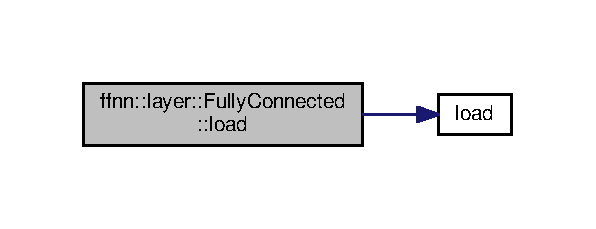
\includegraphics[width=286pt]{classffnn_1_1layer_1_1_fully_connected_a1ff2a601cdf315ce46a2812b4e6fe354_cgraph}
\end{center}
\end{figure}


\hypertarget{classffnn_1_1layer_1_1_fully_connected_aaeb55e214173a632b297d3ddac76fc24}{\index{ffnn\-::layer\-::\-Fully\-Connected@{ffnn\-::layer\-::\-Fully\-Connected}!reset@{reset}}
\index{reset@{reset}!ffnn::layer::FullyConnected@{ffnn\-::layer\-::\-Fully\-Connected}}
\subsubsection[{reset}]{\setlength{\rightskip}{0pt plus 5cm}template$<$typename Value\-Type , F\-F\-N\-N\-\_\-\-S\-I\-Z\-E\-\_\-\-T\-Y\-P\-E Inputs\-At\-Compile\-Time, F\-F\-N\-N\-\_\-\-S\-I\-Z\-E\-\_\-\-T\-Y\-P\-E Outputs\-At\-Compile\-Time, typename \-\_\-\-Hidden\-Layer\-Shape $>$ void {\bf ffnn\-::layer\-::\-Fully\-Connected}$<$ Value\-Type, Inputs\-At\-Compile\-Time, Outputs\-At\-Compile\-Time, \-\_\-\-Hidden\-Layer\-Shape $>$\-::reset (
\begin{DoxyParamCaption}
{}
\end{DoxyParamCaption}
)}}\label{classffnn_1_1layer_1_1_fully_connected_aaeb55e214173a632b297d3ddac76fc24}


Reset weights and biases. 

\hypertarget{classffnn_1_1layer_1_1_fully_connected_a7c79eb99c638b61f76ea34b725c0aeef}{\index{ffnn\-::layer\-::\-Fully\-Connected@{ffnn\-::layer\-::\-Fully\-Connected}!save@{save}}
\index{save@{save}!ffnn::layer::FullyConnected@{ffnn\-::layer\-::\-Fully\-Connected}}
\subsubsection[{save}]{\setlength{\rightskip}{0pt plus 5cm}template$<$typename Value\-Type, F\-F\-N\-N\-\_\-\-S\-I\-Z\-E\-\_\-\-T\-Y\-P\-E Inputs\-At\-Compile\-Time = Eigen\-::\-Dynamic, F\-F\-N\-N\-\_\-\-S\-I\-Z\-E\-\_\-\-T\-Y\-P\-E Outputs\-At\-Compile\-Time = Eigen\-::\-Dynamic, typename \-\_\-\-Hidden\-Layer\-Shape = hidden\-\_\-layer\-\_\-shape$<$\-Inputs\-At\-Compile\-Time, 1, Outputs\-At\-Compile\-Time, 1$>$$>$ void {\bf ffnn\-::layer\-::\-Fully\-Connected}$<$ Value\-Type, Inputs\-At\-Compile\-Time, Outputs\-At\-Compile\-Time, \-\_\-\-Hidden\-Layer\-Shape $>$\-::save (
\begin{DoxyParamCaption}
\item[{{\bf Output\-Archive} \&}]{ar, }
\item[{{\bf Version\-Type}}]{version}
\end{DoxyParamCaption}
) const\hspace{0.3cm}{\ttfamily [protected]}, {\ttfamily [virtual]}}}\label{classffnn_1_1layer_1_1_fully_connected_a7c79eb99c638b61f76ea34b725c0aeef}


Save serialize. 



Reimplemented from \hyperlink{classffnn_1_1internal_1_1_unique_a21fd15cd137dd1cccd23a57fb45649f4}{ffnn\-::internal\-::\-Unique}.



Here is the call graph for this function\-:\nopagebreak
\begin{figure}[H]
\begin{center}
\leavevmode
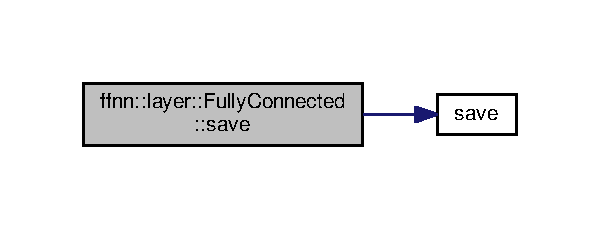
\includegraphics[width=288pt]{classffnn_1_1layer_1_1_fully_connected_a7c79eb99c638b61f76ea34b725c0aeef_cgraph}
\end{center}
\end{figure}


\hypertarget{classffnn_1_1layer_1_1_fully_connected_ae57e6eedc1808825635a1c04aa018992}{\index{ffnn\-::layer\-::\-Fully\-Connected@{ffnn\-::layer\-::\-Fully\-Connected}!set\-Optimizer@{set\-Optimizer}}
\index{set\-Optimizer@{set\-Optimizer}!ffnn::layer::FullyConnected@{ffnn\-::layer\-::\-Fully\-Connected}}
\subsubsection[{set\-Optimizer}]{\setlength{\rightskip}{0pt plus 5cm}template$<$typename Value\-Type , F\-F\-N\-N\-\_\-\-S\-I\-Z\-E\-\_\-\-T\-Y\-P\-E Inputs\-At\-Compile\-Time, F\-F\-N\-N\-\_\-\-S\-I\-Z\-E\-\_\-\-T\-Y\-P\-E Outputs\-At\-Compile\-Time, typename \-\_\-\-Hidden\-Layer\-Shape $>$ void {\bf ffnn\-::layer\-::\-Fully\-Connected}$<$ Value\-Type, Inputs\-At\-Compile\-Time, Outputs\-At\-Compile\-Time, \-\_\-\-Hidden\-Layer\-Shape $>$\-::set\-Optimizer (
\begin{DoxyParamCaption}
\item[{typename {\bf Optimizer\-::\-Ptr}}]{opt}
\end{DoxyParamCaption}
)}}\label{classffnn_1_1layer_1_1_fully_connected_ae57e6eedc1808825635a1c04aa018992}


Sets an optimizer used update network weights during back-\/propagation. 


\begin{DoxyParams}{Parameters}
{\em opt} & optimizer to set \\
\hline
\end{DoxyParams}
\begin{DoxyWarning}{Warning}
{\ttfamily backward} and {\ttfamily update} methods are expected to throw if an optimizer has not been set explicitly 
\end{DoxyWarning}
\hypertarget{classffnn_1_1layer_1_1_fully_connected_a7dd4dbe010c3d290c131b21b35f6301e}{\index{ffnn\-::layer\-::\-Fully\-Connected@{ffnn\-::layer\-::\-Fully\-Connected}!update@{update}}
\index{update@{update}!ffnn::layer::FullyConnected@{ffnn\-::layer\-::\-Fully\-Connected}}
\subsubsection[{update}]{\setlength{\rightskip}{0pt plus 5cm}template$<$typename Value\-Type , F\-F\-N\-N\-\_\-\-S\-I\-Z\-E\-\_\-\-T\-Y\-P\-E Inputs\-At\-Compile\-Time, F\-F\-N\-N\-\_\-\-S\-I\-Z\-E\-\_\-\-T\-Y\-P\-E Outputs\-At\-Compile\-Time, typename \-\_\-\-Hidden\-Layer\-Shape $>$ bool {\bf ffnn\-::layer\-::\-Fully\-Connected}$<$ Value\-Type, Inputs\-At\-Compile\-Time, Outputs\-At\-Compile\-Time, \-\_\-\-Hidden\-Layer\-Shape $>$\-::update (
\begin{DoxyParamCaption}
{}
\end{DoxyParamCaption}
)\hspace{0.3cm}{\ttfamily [virtual]}}}\label{classffnn_1_1layer_1_1_fully_connected_a7dd4dbe010c3d290c131b21b35f6301e}


Applies accumulated layer weight updates computed during optimization. 


\begin{DoxyRetVals}{Return values}
{\em true} & if weight update succeeded \\
\hline
{\em false} & otherwise \\
\hline
\end{DoxyRetVals}
\begin{DoxyWarning}{Warning}
Will throw if an optimizer has not been associated with this layer 
\end{DoxyWarning}
\begin{DoxySeeAlso}{See Also}
\hyperlink{classffnn_1_1layer_1_1_fully_connected_ae57e6eedc1808825635a1c04aa018992}{set\-Optimizer} 
\end{DoxySeeAlso}


Implements \hyperlink{classffnn_1_1layer_1_1_hidden_ac95dceacf1a0ea65674fb269a48730fb}{ffnn\-::layer\-::\-Hidden$<$ Value\-Type, \-\_\-\-Hidden\-Layer\-Shape $>$}.



The documentation for this class was generated from the following files\-:\begin{DoxyCompactItemize}
\item 
/home/briancairl/packages/src/ffnn-\/cpp/ffnn/include/ffnn/layer/\hyperlink{fully__connected_8h}{fully\-\_\-connected.\-h}\item 
/home/briancairl/packages/src/ffnn-\/cpp/ffnn/include/ffnn/impl/layer/\hyperlink{impl_2layer_2fully__connected_8hpp}{fully\-\_\-connected.\-hpp}\end{DoxyCompactItemize}

\hypertarget{classffnn_1_1optimizer_1_1_gradient_descent}{\section{ffnn\-:\-:optimizer\-:\-:Gradient\-Descent$<$ Layer\-Type, Loss\-Fn $>$ Class Template Reference}
\label{classffnn_1_1optimizer_1_1_gradient_descent}\index{ffnn\-::optimizer\-::\-Gradient\-Descent$<$ Layer\-Type, Loss\-Fn $>$@{ffnn\-::optimizer\-::\-Gradient\-Descent$<$ Layer\-Type, Loss\-Fn $>$}}
}


{\ttfamily \#include \char`\"{}fwd.\-h\char`\"{}}



The documentation for this class was generated from the following file\-:\begin{DoxyCompactItemize}
\item 
/home/briancairl/packages/src/ffnn-\/cpp/ffnn/include/ffnn/optimizer/\hyperlink{fwd_8h}{fwd.\-h}\end{DoxyCompactItemize}

\hypertarget{classffnn_1_1optimizer_1_1_gradient_descent_3_01layer_1_1_convolution_3_01_t_a_r_g_s_01_4_01_4}{\section{ffnn\-:\-:optimizer\-:\-:Gradient\-Descent$<$ layer\-:\-:Convolution$<$ T\-A\-R\-G\-S $>$ $>$ Class Template Reference}
\label{classffnn_1_1optimizer_1_1_gradient_descent_3_01layer_1_1_convolution_3_01_t_a_r_g_s_01_4_01_4}\index{ffnn\-::optimizer\-::\-Gradient\-Descent$<$ layer\-::\-Convolution$<$ T\-A\-R\-G\-S $>$ $>$@{ffnn\-::optimizer\-::\-Gradient\-Descent$<$ layer\-::\-Convolution$<$ T\-A\-R\-G\-S $>$ $>$}}
}


{\ttfamily \#include \char`\"{}convolution.\-hpp\char`\"{}}



Inheritance diagram for ffnn\-:\-:optimizer\-:\-:Gradient\-Descent$<$ layer\-:\-:Convolution$<$ T\-A\-R\-G\-S $>$ $>$\-:\nopagebreak
\begin{figure}[H]
\begin{center}
\leavevmode
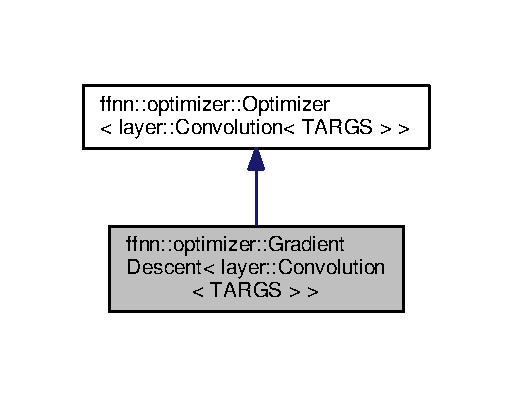
\includegraphics[width=246pt]{classffnn_1_1optimizer_1_1_gradient_descent_3_01layer_1_1_convolution_3_01_t_a_r_g_s_01_4_01_4__inherit__graph}
\end{center}
\end{figure}


Collaboration diagram for ffnn\-:\-:optimizer\-:\-:Gradient\-Descent$<$ layer\-:\-:Convolution$<$ T\-A\-R\-G\-S $>$ $>$\-:\nopagebreak
\begin{figure}[H]
\begin{center}
\leavevmode
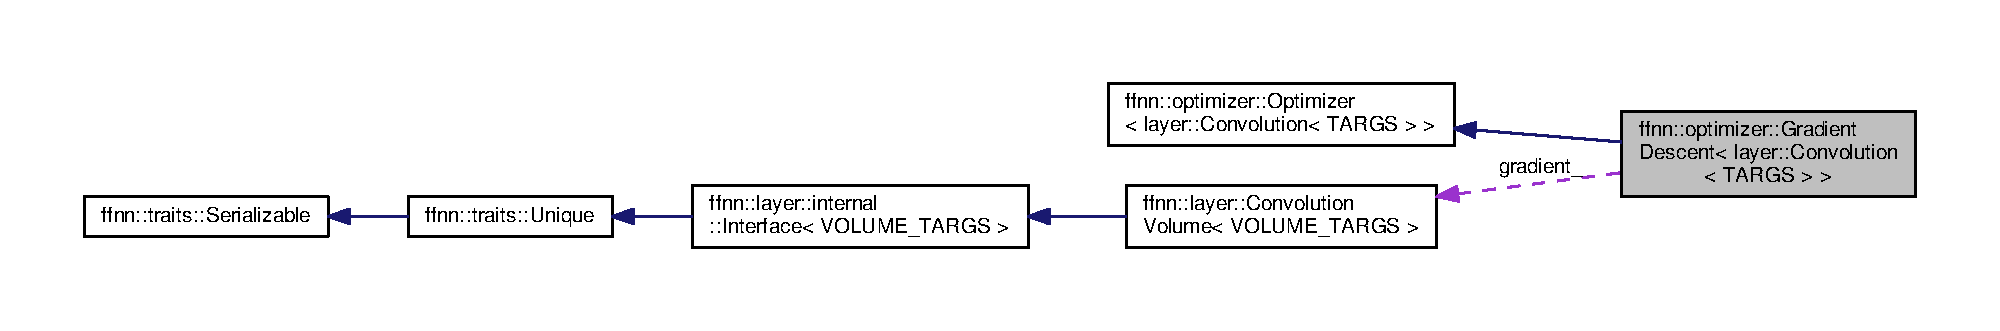
\includegraphics[width=246pt]{classffnn_1_1optimizer_1_1_gradient_descent_3_01layer_1_1_convolution_3_01_t_a_r_g_s_01_4_01_4__coll__graph}
\end{center}
\end{figure}
\subsection*{Public Types}
\begin{DoxyCompactItemize}
\item 
typedef \hyperlink{classffnn_1_1layer_1_1_convolution}{layer\-::\-Convolution}$<$ \hyperlink{local__convolution_8hpp_a005b9b79411aa786124330e813a99057}{T\-A\-R\-G\-S} $>$ \hyperlink{classffnn_1_1optimizer_1_1_gradient_descent_3_01layer_1_1_convolution_3_01_t_a_r_g_s_01_4_01_4_a4b4e11ad265dd0fba9010b60d6cea09b}{Layer\-Type}
\begin{DoxyCompactList}\small\item\em Layer type standardization. \end{DoxyCompactList}\item 
typedef Layer\-Type\-::\-Scalar\-Type \hyperlink{classffnn_1_1optimizer_1_1_gradient_descent_3_01layer_1_1_convolution_3_01_t_a_r_g_s_01_4_01_4_a041c24c2e8946fd3cc93f9094930250e}{Scalar\-Type}
\begin{DoxyCompactList}\small\item\em Scalar type standardization. \end{DoxyCompactList}\item 
typedef Layer\-Type\-::\-Size\-Type \hyperlink{classffnn_1_1optimizer_1_1_gradient_descent_3_01layer_1_1_convolution_3_01_t_a_r_g_s_01_4_01_4_a02796dc7270c0180e5e0cfa57e015dde}{Size\-Type}
\begin{DoxyCompactList}\small\item\em Size type standardization. \end{DoxyCompactList}\item 
typedef Layer\-Type\-::\-Offset\-Type \hyperlink{classffnn_1_1optimizer_1_1_gradient_descent_3_01layer_1_1_convolution_3_01_t_a_r_g_s_01_4_01_4_adeba594318f6939122d3e0edb069d6d6}{Offset\-Type}
\begin{DoxyCompactList}\small\item\em Offset type standardization. \end{DoxyCompactList}\item 
typedef Layer\-Type\-::\-Input\-Block\-Type \hyperlink{classffnn_1_1optimizer_1_1_gradient_descent_3_01layer_1_1_convolution_3_01_t_a_r_g_s_01_4_01_4_a52ff7f9db21ea50795ccbc475a3cc643}{Input\-Block\-Type}
\begin{DoxyCompactList}\small\item\em Matrix type standardization. \end{DoxyCompactList}\item 
typedef Layer\-Type\-::\-Output\-Block\-Type \hyperlink{classffnn_1_1optimizer_1_1_gradient_descent_3_01layer_1_1_convolution_3_01_t_a_r_g_s_01_4_01_4_a24c60e1a115ce2e27567a5b068eaf0a8}{Output\-Block\-Type}
\begin{DoxyCompactList}\small\item\em Matrix type standardization. \end{DoxyCompactList}\item 
typedef Layer\-Type\-::\-Parameters\-Type \hyperlink{classffnn_1_1optimizer_1_1_gradient_descent_3_01layer_1_1_convolution_3_01_t_a_r_g_s_01_4_01_4_a0bbe4560ab81eacf8e75ac5510ad696e}{Parameters\-Type}
\begin{DoxyCompactList}\small\item\em Parameter collection type standardization. \end{DoxyCompactList}\end{DoxyCompactItemize}
\subsection*{Public Member Functions}
\begin{DoxyCompactItemize}
\item 
\hyperlink{classffnn_1_1optimizer_1_1_gradient_descent_3_01layer_1_1_convolution_3_01_t_a_r_g_s_01_4_01_4_a480650884dc02d9994f2341b6236bcf8}{Gradient\-Descent} (\hyperlink{classffnn_1_1optimizer_1_1_gradient_descent_3_01layer_1_1_convolution_3_01_t_a_r_g_s_01_4_01_4_a041c24c2e8946fd3cc93f9094930250e}{Scalar\-Type} lr)
\begin{DoxyCompactList}\small\item\em Setup constructor. \end{DoxyCompactList}\item 
virtual \hyperlink{classffnn_1_1optimizer_1_1_gradient_descent_3_01layer_1_1_convolution_3_01_t_a_r_g_s_01_4_01_4_a173580134cb115ced38660a1cdeca830}{$\sim$\-Gradient\-Descent} ()
\item 
void \hyperlink{classffnn_1_1optimizer_1_1_gradient_descent_3_01layer_1_1_convolution_3_01_t_a_r_g_s_01_4_01_4_a6dbb9707492c05e512163935ac7330c9}{initialize} (\hyperlink{classffnn_1_1optimizer_1_1_gradient_descent_3_01layer_1_1_convolution_3_01_t_a_r_g_s_01_4_01_4_a4b4e11ad265dd0fba9010b60d6cea09b}{Layer\-Type} \&layer)
\begin{DoxyCompactList}\small\item\em Initializes the \hyperlink{classffnn_1_1optimizer_1_1_optimizer}{Optimizer}. \end{DoxyCompactList}\item 
void \hyperlink{classffnn_1_1optimizer_1_1_gradient_descent_3_01layer_1_1_convolution_3_01_t_a_r_g_s_01_4_01_4_ab5761e35397a5d346dc81c225af9402a}{reset} (\hyperlink{classffnn_1_1optimizer_1_1_gradient_descent_3_01layer_1_1_convolution_3_01_t_a_r_g_s_01_4_01_4_a4b4e11ad265dd0fba9010b60d6cea09b}{Layer\-Type} \&layer)
\begin{DoxyCompactList}\small\item\em Resetrs persistent \hyperlink{classffnn_1_1optimizer_1_1_optimizer}{Optimizer} states. \end{DoxyCompactList}\item 
bool \hyperlink{classffnn_1_1optimizer_1_1_gradient_descent_3_01layer_1_1_convolution_3_01_t_a_r_g_s_01_4_01_4_a873062535938aebab53a62d93f3e7db7}{forward} (\hyperlink{classffnn_1_1optimizer_1_1_gradient_descent_3_01layer_1_1_convolution_3_01_t_a_r_g_s_01_4_01_4_a4b4e11ad265dd0fba9010b60d6cea09b}{Layer\-Type} \&layer)
\begin{DoxyCompactList}\small\item\em Computes one forward optimization update step. \end{DoxyCompactList}\item 
bool \hyperlink{classffnn_1_1optimizer_1_1_gradient_descent_3_01layer_1_1_convolution_3_01_t_a_r_g_s_01_4_01_4_a8b37b876d0d861623d36764a37e3e6e2}{backward} (\hyperlink{classffnn_1_1optimizer_1_1_gradient_descent_3_01layer_1_1_convolution_3_01_t_a_r_g_s_01_4_01_4_a4b4e11ad265dd0fba9010b60d6cea09b}{Layer\-Type} \&layer)
\begin{DoxyCompactList}\small\item\em Computes optimization step during backward propogation. \end{DoxyCompactList}\item 
bool \hyperlink{classffnn_1_1optimizer_1_1_gradient_descent_3_01layer_1_1_convolution_3_01_t_a_r_g_s_01_4_01_4_a3cbbcd9490ff52ee7984bfcb17db4ee1}{update} (\hyperlink{classffnn_1_1optimizer_1_1_gradient_descent_3_01layer_1_1_convolution_3_01_t_a_r_g_s_01_4_01_4_a4b4e11ad265dd0fba9010b60d6cea09b}{Layer\-Type} \&layer)
\begin{DoxyCompactList}\small\item\em Applies optimization update. \end{DoxyCompactList}\end{DoxyCompactItemize}
\subsection*{Protected Attributes}
\begin{DoxyCompactItemize}
\item 
\hyperlink{classffnn_1_1optimizer_1_1_gradient_descent_3_01layer_1_1_convolution_3_01_t_a_r_g_s_01_4_01_4_a041c24c2e8946fd3cc93f9094930250e}{Scalar\-Type} \hyperlink{classffnn_1_1optimizer_1_1_gradient_descent_3_01layer_1_1_convolution_3_01_t_a_r_g_s_01_4_01_4_a054941817564001aa5d455a9fe41262e}{lr\-\_\-}
\begin{DoxyCompactList}\small\item\em Learning rate. \end{DoxyCompactList}\item 
\hyperlink{classffnn_1_1optimizer_1_1_gradient_descent_3_01layer_1_1_convolution_3_01_t_a_r_g_s_01_4_01_4_a0bbe4560ab81eacf8e75ac5510ad696e}{Parameters\-Type} \hyperlink{classffnn_1_1optimizer_1_1_gradient_descent_3_01layer_1_1_convolution_3_01_t_a_r_g_s_01_4_01_4_a2e5183618894852cb53de619372d6ad1}{gradient\-\_\-}
\begin{DoxyCompactList}\small\item\em Total parameter gradient. \end{DoxyCompactList}\item 
\hyperlink{classffnn_1_1optimizer_1_1_gradient_descent_3_01layer_1_1_convolution_3_01_t_a_r_g_s_01_4_01_4_a52ff7f9db21ea50795ccbc475a3cc643}{Input\-Block\-Type} \hyperlink{classffnn_1_1optimizer_1_1_gradient_descent_3_01layer_1_1_convolution_3_01_t_a_r_g_s_01_4_01_4_afb2c039078e26446400314336dc24482}{prev\-\_\-input\-\_\-}
\begin{DoxyCompactList}\small\item\em Previous input. \end{DoxyCompactList}\end{DoxyCompactItemize}


\subsection{Member Typedef Documentation}
\hypertarget{classffnn_1_1optimizer_1_1_gradient_descent_3_01layer_1_1_convolution_3_01_t_a_r_g_s_01_4_01_4_a52ff7f9db21ea50795ccbc475a3cc643}{\index{ffnn\-::optimizer\-::\-Gradient\-Descent$<$ layer\-::\-Convolution$<$ T\-A\-R\-G\-S $>$ $>$@{ffnn\-::optimizer\-::\-Gradient\-Descent$<$ layer\-::\-Convolution$<$ T\-A\-R\-G\-S $>$ $>$}!Input\-Block\-Type@{Input\-Block\-Type}}
\index{Input\-Block\-Type@{Input\-Block\-Type}!ffnn::optimizer::GradientDescent< layer::Convolution< TARGS > >@{ffnn\-::optimizer\-::\-Gradient\-Descent$<$ layer\-::\-Convolution$<$ T\-A\-R\-G\-S $>$ $>$}}
\subsubsection[{Input\-Block\-Type}]{\setlength{\rightskip}{0pt plus 5cm}typedef Layer\-Type\-::\-Input\-Block\-Type {\bf ffnn\-::optimizer\-::\-Gradient\-Descent}$<$ {\bf layer\-::\-Convolution}$<$ {\bf T\-A\-R\-G\-S} $>$ $>$\-::{\bf Input\-Block\-Type}}}\label{classffnn_1_1optimizer_1_1_gradient_descent_3_01layer_1_1_convolution_3_01_t_a_r_g_s_01_4_01_4_a52ff7f9db21ea50795ccbc475a3cc643}


Matrix type standardization. 

\hypertarget{classffnn_1_1optimizer_1_1_gradient_descent_3_01layer_1_1_convolution_3_01_t_a_r_g_s_01_4_01_4_a4b4e11ad265dd0fba9010b60d6cea09b}{\index{ffnn\-::optimizer\-::\-Gradient\-Descent$<$ layer\-::\-Convolution$<$ T\-A\-R\-G\-S $>$ $>$@{ffnn\-::optimizer\-::\-Gradient\-Descent$<$ layer\-::\-Convolution$<$ T\-A\-R\-G\-S $>$ $>$}!Layer\-Type@{Layer\-Type}}
\index{Layer\-Type@{Layer\-Type}!ffnn::optimizer::GradientDescent< layer::Convolution< TARGS > >@{ffnn\-::optimizer\-::\-Gradient\-Descent$<$ layer\-::\-Convolution$<$ T\-A\-R\-G\-S $>$ $>$}}
\subsubsection[{Layer\-Type}]{\setlength{\rightskip}{0pt plus 5cm}typedef {\bf layer\-::\-Convolution}$<${\bf T\-A\-R\-G\-S}$>$ {\bf ffnn\-::optimizer\-::\-Gradient\-Descent}$<$ {\bf layer\-::\-Convolution}$<$ {\bf T\-A\-R\-G\-S} $>$ $>$\-::{\bf Layer\-Type}}}\label{classffnn_1_1optimizer_1_1_gradient_descent_3_01layer_1_1_convolution_3_01_t_a_r_g_s_01_4_01_4_a4b4e11ad265dd0fba9010b60d6cea09b}


Layer type standardization. 

\hypertarget{classffnn_1_1optimizer_1_1_gradient_descent_3_01layer_1_1_convolution_3_01_t_a_r_g_s_01_4_01_4_adeba594318f6939122d3e0edb069d6d6}{\index{ffnn\-::optimizer\-::\-Gradient\-Descent$<$ layer\-::\-Convolution$<$ T\-A\-R\-G\-S $>$ $>$@{ffnn\-::optimizer\-::\-Gradient\-Descent$<$ layer\-::\-Convolution$<$ T\-A\-R\-G\-S $>$ $>$}!Offset\-Type@{Offset\-Type}}
\index{Offset\-Type@{Offset\-Type}!ffnn::optimizer::GradientDescent< layer::Convolution< TARGS > >@{ffnn\-::optimizer\-::\-Gradient\-Descent$<$ layer\-::\-Convolution$<$ T\-A\-R\-G\-S $>$ $>$}}
\subsubsection[{Offset\-Type}]{\setlength{\rightskip}{0pt plus 5cm}typedef Layer\-Type\-::\-Offset\-Type {\bf ffnn\-::optimizer\-::\-Gradient\-Descent}$<$ {\bf layer\-::\-Convolution}$<$ {\bf T\-A\-R\-G\-S} $>$ $>$\-::{\bf Offset\-Type}}}\label{classffnn_1_1optimizer_1_1_gradient_descent_3_01layer_1_1_convolution_3_01_t_a_r_g_s_01_4_01_4_adeba594318f6939122d3e0edb069d6d6}


Offset type standardization. 

\hypertarget{classffnn_1_1optimizer_1_1_gradient_descent_3_01layer_1_1_convolution_3_01_t_a_r_g_s_01_4_01_4_a24c60e1a115ce2e27567a5b068eaf0a8}{\index{ffnn\-::optimizer\-::\-Gradient\-Descent$<$ layer\-::\-Convolution$<$ T\-A\-R\-G\-S $>$ $>$@{ffnn\-::optimizer\-::\-Gradient\-Descent$<$ layer\-::\-Convolution$<$ T\-A\-R\-G\-S $>$ $>$}!Output\-Block\-Type@{Output\-Block\-Type}}
\index{Output\-Block\-Type@{Output\-Block\-Type}!ffnn::optimizer::GradientDescent< layer::Convolution< TARGS > >@{ffnn\-::optimizer\-::\-Gradient\-Descent$<$ layer\-::\-Convolution$<$ T\-A\-R\-G\-S $>$ $>$}}
\subsubsection[{Output\-Block\-Type}]{\setlength{\rightskip}{0pt plus 5cm}typedef Layer\-Type\-::\-Output\-Block\-Type {\bf ffnn\-::optimizer\-::\-Gradient\-Descent}$<$ {\bf layer\-::\-Convolution}$<$ {\bf T\-A\-R\-G\-S} $>$ $>$\-::{\bf Output\-Block\-Type}}}\label{classffnn_1_1optimizer_1_1_gradient_descent_3_01layer_1_1_convolution_3_01_t_a_r_g_s_01_4_01_4_a24c60e1a115ce2e27567a5b068eaf0a8}


Matrix type standardization. 

\hypertarget{classffnn_1_1optimizer_1_1_gradient_descent_3_01layer_1_1_convolution_3_01_t_a_r_g_s_01_4_01_4_a0bbe4560ab81eacf8e75ac5510ad696e}{\index{ffnn\-::optimizer\-::\-Gradient\-Descent$<$ layer\-::\-Convolution$<$ T\-A\-R\-G\-S $>$ $>$@{ffnn\-::optimizer\-::\-Gradient\-Descent$<$ layer\-::\-Convolution$<$ T\-A\-R\-G\-S $>$ $>$}!Parameters\-Type@{Parameters\-Type}}
\index{Parameters\-Type@{Parameters\-Type}!ffnn::optimizer::GradientDescent< layer::Convolution< TARGS > >@{ffnn\-::optimizer\-::\-Gradient\-Descent$<$ layer\-::\-Convolution$<$ T\-A\-R\-G\-S $>$ $>$}}
\subsubsection[{Parameters\-Type}]{\setlength{\rightskip}{0pt plus 5cm}typedef Layer\-Type\-::\-Parameters\-Type {\bf ffnn\-::optimizer\-::\-Gradient\-Descent}$<$ {\bf layer\-::\-Convolution}$<$ {\bf T\-A\-R\-G\-S} $>$ $>$\-::{\bf Parameters\-Type}}}\label{classffnn_1_1optimizer_1_1_gradient_descent_3_01layer_1_1_convolution_3_01_t_a_r_g_s_01_4_01_4_a0bbe4560ab81eacf8e75ac5510ad696e}


Parameter collection type standardization. 

\hypertarget{classffnn_1_1optimizer_1_1_gradient_descent_3_01layer_1_1_convolution_3_01_t_a_r_g_s_01_4_01_4_a041c24c2e8946fd3cc93f9094930250e}{\index{ffnn\-::optimizer\-::\-Gradient\-Descent$<$ layer\-::\-Convolution$<$ T\-A\-R\-G\-S $>$ $>$@{ffnn\-::optimizer\-::\-Gradient\-Descent$<$ layer\-::\-Convolution$<$ T\-A\-R\-G\-S $>$ $>$}!Scalar\-Type@{Scalar\-Type}}
\index{Scalar\-Type@{Scalar\-Type}!ffnn::optimizer::GradientDescent< layer::Convolution< TARGS > >@{ffnn\-::optimizer\-::\-Gradient\-Descent$<$ layer\-::\-Convolution$<$ T\-A\-R\-G\-S $>$ $>$}}
\subsubsection[{Scalar\-Type}]{\setlength{\rightskip}{0pt plus 5cm}typedef Layer\-Type\-::\-Scalar\-Type {\bf ffnn\-::optimizer\-::\-Gradient\-Descent}$<$ {\bf layer\-::\-Convolution}$<$ {\bf T\-A\-R\-G\-S} $>$ $>$\-::{\bf Scalar\-Type}}}\label{classffnn_1_1optimizer_1_1_gradient_descent_3_01layer_1_1_convolution_3_01_t_a_r_g_s_01_4_01_4_a041c24c2e8946fd3cc93f9094930250e}


Scalar type standardization. 

\hypertarget{classffnn_1_1optimizer_1_1_gradient_descent_3_01layer_1_1_convolution_3_01_t_a_r_g_s_01_4_01_4_a02796dc7270c0180e5e0cfa57e015dde}{\index{ffnn\-::optimizer\-::\-Gradient\-Descent$<$ layer\-::\-Convolution$<$ T\-A\-R\-G\-S $>$ $>$@{ffnn\-::optimizer\-::\-Gradient\-Descent$<$ layer\-::\-Convolution$<$ T\-A\-R\-G\-S $>$ $>$}!Size\-Type@{Size\-Type}}
\index{Size\-Type@{Size\-Type}!ffnn::optimizer::GradientDescent< layer::Convolution< TARGS > >@{ffnn\-::optimizer\-::\-Gradient\-Descent$<$ layer\-::\-Convolution$<$ T\-A\-R\-G\-S $>$ $>$}}
\subsubsection[{Size\-Type}]{\setlength{\rightskip}{0pt plus 5cm}typedef Layer\-Type\-::\-Size\-Type {\bf ffnn\-::optimizer\-::\-Gradient\-Descent}$<$ {\bf layer\-::\-Convolution}$<$ {\bf T\-A\-R\-G\-S} $>$ $>$\-::{\bf Size\-Type}}}\label{classffnn_1_1optimizer_1_1_gradient_descent_3_01layer_1_1_convolution_3_01_t_a_r_g_s_01_4_01_4_a02796dc7270c0180e5e0cfa57e015dde}


Size type standardization. 



\subsection{Constructor \& Destructor Documentation}
\hypertarget{classffnn_1_1optimizer_1_1_gradient_descent_3_01layer_1_1_convolution_3_01_t_a_r_g_s_01_4_01_4_a480650884dc02d9994f2341b6236bcf8}{\index{ffnn\-::optimizer\-::\-Gradient\-Descent$<$ layer\-::\-Convolution$<$ T\-A\-R\-G\-S $>$ $>$@{ffnn\-::optimizer\-::\-Gradient\-Descent$<$ layer\-::\-Convolution$<$ T\-A\-R\-G\-S $>$ $>$}!Gradient\-Descent@{Gradient\-Descent}}
\index{Gradient\-Descent@{Gradient\-Descent}!ffnn::optimizer::GradientDescent< layer::Convolution< TARGS > >@{ffnn\-::optimizer\-::\-Gradient\-Descent$<$ layer\-::\-Convolution$<$ T\-A\-R\-G\-S $>$ $>$}}
\subsubsection[{Gradient\-Descent}]{\setlength{\rightskip}{0pt plus 5cm}{\bf ffnn\-::optimizer\-::\-Gradient\-Descent}$<$ {\bf layer\-::\-Convolution}$<$ {\bf T\-A\-R\-G\-S} $>$ $>$\-::{\bf Gradient\-Descent} (
\begin{DoxyParamCaption}
\item[{{\bf Scalar\-Type}}]{lr}
\end{DoxyParamCaption}
)\hspace{0.3cm}{\ttfamily [inline]}, {\ttfamily [explicit]}}}\label{classffnn_1_1optimizer_1_1_gradient_descent_3_01layer_1_1_convolution_3_01_t_a_r_g_s_01_4_01_4_a480650884dc02d9994f2341b6236bcf8}


Setup constructor. 


\begin{DoxyParams}{Parameters}
{\em lr} & Learning rate \\
\hline
\end{DoxyParams}
\hypertarget{classffnn_1_1optimizer_1_1_gradient_descent_3_01layer_1_1_convolution_3_01_t_a_r_g_s_01_4_01_4_a173580134cb115ced38660a1cdeca830}{\index{ffnn\-::optimizer\-::\-Gradient\-Descent$<$ layer\-::\-Convolution$<$ T\-A\-R\-G\-S $>$ $>$@{ffnn\-::optimizer\-::\-Gradient\-Descent$<$ layer\-::\-Convolution$<$ T\-A\-R\-G\-S $>$ $>$}!$\sim$\-Gradient\-Descent@{$\sim$\-Gradient\-Descent}}
\index{$\sim$\-Gradient\-Descent@{$\sim$\-Gradient\-Descent}!ffnn::optimizer::GradientDescent< layer::Convolution< TARGS > >@{ffnn\-::optimizer\-::\-Gradient\-Descent$<$ layer\-::\-Convolution$<$ T\-A\-R\-G\-S $>$ $>$}}
\subsubsection[{$\sim$\-Gradient\-Descent}]{\setlength{\rightskip}{0pt plus 5cm}virtual {\bf ffnn\-::optimizer\-::\-Gradient\-Descent}$<$ {\bf layer\-::\-Convolution}$<$ {\bf T\-A\-R\-G\-S} $>$ $>$\-::$\sim${\bf Gradient\-Descent} (
\begin{DoxyParamCaption}
{}
\end{DoxyParamCaption}
)\hspace{0.3cm}{\ttfamily [inline]}, {\ttfamily [virtual]}}}\label{classffnn_1_1optimizer_1_1_gradient_descent_3_01layer_1_1_convolution_3_01_t_a_r_g_s_01_4_01_4_a173580134cb115ced38660a1cdeca830}


\subsection{Member Function Documentation}
\hypertarget{classffnn_1_1optimizer_1_1_gradient_descent_3_01layer_1_1_convolution_3_01_t_a_r_g_s_01_4_01_4_a8b37b876d0d861623d36764a37e3e6e2}{\index{ffnn\-::optimizer\-::\-Gradient\-Descent$<$ layer\-::\-Convolution$<$ T\-A\-R\-G\-S $>$ $>$@{ffnn\-::optimizer\-::\-Gradient\-Descent$<$ layer\-::\-Convolution$<$ T\-A\-R\-G\-S $>$ $>$}!backward@{backward}}
\index{backward@{backward}!ffnn::optimizer::GradientDescent< layer::Convolution< TARGS > >@{ffnn\-::optimizer\-::\-Gradient\-Descent$<$ layer\-::\-Convolution$<$ T\-A\-R\-G\-S $>$ $>$}}
\subsubsection[{backward}]{\setlength{\rightskip}{0pt plus 5cm}bool {\bf ffnn\-::optimizer\-::\-Gradient\-Descent}$<$ {\bf layer\-::\-Convolution}$<$ {\bf T\-A\-R\-G\-S} $>$ $>$\-::backward (
\begin{DoxyParamCaption}
\item[{{\bf Layer\-Type} \&}]{layer}
\end{DoxyParamCaption}
)\hspace{0.3cm}{\ttfamily [inline]}, {\ttfamily [virtual]}}}\label{classffnn_1_1optimizer_1_1_gradient_descent_3_01layer_1_1_convolution_3_01_t_a_r_g_s_01_4_01_4_a8b37b876d0d861623d36764a37e3e6e2}


Computes optimization step during backward propogation. 


\begin{DoxyParams}[1]{Parameters}
\mbox{\tt in,out}  & {\em layer} & Layer to optimize \\
\hline
\end{DoxyParams}

\begin{DoxyRetVals}{Return values}
{\em true} & if optimization setp was successful \\
\hline
{\em false} & otherwise \\
\hline
\end{DoxyRetVals}


Implements \hyperlink{classffnn_1_1optimizer_1_1_optimizer_ab1f9b1cae01f93f53ecf7119bedb6369}{ffnn\-::optimizer\-::\-Optimizer$<$ layer\-::\-Convolution$<$ T\-A\-R\-G\-S $>$ $>$}.

\hypertarget{classffnn_1_1optimizer_1_1_gradient_descent_3_01layer_1_1_convolution_3_01_t_a_r_g_s_01_4_01_4_a873062535938aebab53a62d93f3e7db7}{\index{ffnn\-::optimizer\-::\-Gradient\-Descent$<$ layer\-::\-Convolution$<$ T\-A\-R\-G\-S $>$ $>$@{ffnn\-::optimizer\-::\-Gradient\-Descent$<$ layer\-::\-Convolution$<$ T\-A\-R\-G\-S $>$ $>$}!forward@{forward}}
\index{forward@{forward}!ffnn::optimizer::GradientDescent< layer::Convolution< TARGS > >@{ffnn\-::optimizer\-::\-Gradient\-Descent$<$ layer\-::\-Convolution$<$ T\-A\-R\-G\-S $>$ $>$}}
\subsubsection[{forward}]{\setlength{\rightskip}{0pt plus 5cm}bool {\bf ffnn\-::optimizer\-::\-Gradient\-Descent}$<$ {\bf layer\-::\-Convolution}$<$ {\bf T\-A\-R\-G\-S} $>$ $>$\-::forward (
\begin{DoxyParamCaption}
\item[{{\bf Layer\-Type} \&}]{layer}
\end{DoxyParamCaption}
)\hspace{0.3cm}{\ttfamily [inline]}, {\ttfamily [virtual]}}}\label{classffnn_1_1optimizer_1_1_gradient_descent_3_01layer_1_1_convolution_3_01_t_a_r_g_s_01_4_01_4_a873062535938aebab53a62d93f3e7db7}


Computes one forward optimization update step. 


\begin{DoxyParams}[1]{Parameters}
\mbox{\tt in,out}  & {\em layer} & Layer to optimize \\
\hline
\end{DoxyParams}

\begin{DoxyRetVals}{Return values}
{\em true} & if optimization setp was successful \\
\hline
{\em false} & otherwise \\
\hline
\end{DoxyRetVals}


Implements \hyperlink{classffnn_1_1optimizer_1_1_optimizer_a80505cfdeba0a3c8d1db19a2821613f2}{ffnn\-::optimizer\-::\-Optimizer$<$ layer\-::\-Convolution$<$ T\-A\-R\-G\-S $>$ $>$}.

\hypertarget{classffnn_1_1optimizer_1_1_gradient_descent_3_01layer_1_1_convolution_3_01_t_a_r_g_s_01_4_01_4_a6dbb9707492c05e512163935ac7330c9}{\index{ffnn\-::optimizer\-::\-Gradient\-Descent$<$ layer\-::\-Convolution$<$ T\-A\-R\-G\-S $>$ $>$@{ffnn\-::optimizer\-::\-Gradient\-Descent$<$ layer\-::\-Convolution$<$ T\-A\-R\-G\-S $>$ $>$}!initialize@{initialize}}
\index{initialize@{initialize}!ffnn::optimizer::GradientDescent< layer::Convolution< TARGS > >@{ffnn\-::optimizer\-::\-Gradient\-Descent$<$ layer\-::\-Convolution$<$ T\-A\-R\-G\-S $>$ $>$}}
\subsubsection[{initialize}]{\setlength{\rightskip}{0pt plus 5cm}void {\bf ffnn\-::optimizer\-::\-Gradient\-Descent}$<$ {\bf layer\-::\-Convolution}$<$ {\bf T\-A\-R\-G\-S} $>$ $>$\-::initialize (
\begin{DoxyParamCaption}
\item[{{\bf Layer\-Type} \&}]{layer}
\end{DoxyParamCaption}
)\hspace{0.3cm}{\ttfamily [inline]}, {\ttfamily [virtual]}}}\label{classffnn_1_1optimizer_1_1_gradient_descent_3_01layer_1_1_convolution_3_01_t_a_r_g_s_01_4_01_4_a6dbb9707492c05e512163935ac7330c9}


Initializes the \hyperlink{classffnn_1_1optimizer_1_1_optimizer}{Optimizer}. 


\begin{DoxyParams}[1]{Parameters}
\mbox{\tt in,out}  & {\em layer} & Layer to optimize \\
\hline
\end{DoxyParams}


Implements \hyperlink{classffnn_1_1optimizer_1_1_optimizer_a4302b66ba9b013ae4833eca235ff306a}{ffnn\-::optimizer\-::\-Optimizer$<$ layer\-::\-Convolution$<$ T\-A\-R\-G\-S $>$ $>$}.

\hypertarget{classffnn_1_1optimizer_1_1_gradient_descent_3_01layer_1_1_convolution_3_01_t_a_r_g_s_01_4_01_4_ab5761e35397a5d346dc81c225af9402a}{\index{ffnn\-::optimizer\-::\-Gradient\-Descent$<$ layer\-::\-Convolution$<$ T\-A\-R\-G\-S $>$ $>$@{ffnn\-::optimizer\-::\-Gradient\-Descent$<$ layer\-::\-Convolution$<$ T\-A\-R\-G\-S $>$ $>$}!reset@{reset}}
\index{reset@{reset}!ffnn::optimizer::GradientDescent< layer::Convolution< TARGS > >@{ffnn\-::optimizer\-::\-Gradient\-Descent$<$ layer\-::\-Convolution$<$ T\-A\-R\-G\-S $>$ $>$}}
\subsubsection[{reset}]{\setlength{\rightskip}{0pt plus 5cm}void {\bf ffnn\-::optimizer\-::\-Gradient\-Descent}$<$ {\bf layer\-::\-Convolution}$<$ {\bf T\-A\-R\-G\-S} $>$ $>$\-::reset (
\begin{DoxyParamCaption}
\item[{{\bf Layer\-Type} \&}]{layer}
\end{DoxyParamCaption}
)\hspace{0.3cm}{\ttfamily [inline]}, {\ttfamily [virtual]}}}\label{classffnn_1_1optimizer_1_1_gradient_descent_3_01layer_1_1_convolution_3_01_t_a_r_g_s_01_4_01_4_ab5761e35397a5d346dc81c225af9402a}


Resetrs persistent \hyperlink{classffnn_1_1optimizer_1_1_optimizer}{Optimizer} states. 


\begin{DoxyParams}[1]{Parameters}
\mbox{\tt in,out}  & {\em layer} & Layer to optimize \\
\hline
\end{DoxyParams}


Implements \hyperlink{classffnn_1_1optimizer_1_1_optimizer_ade04e7582eb7b833713a9bd33e0e8346}{ffnn\-::optimizer\-::\-Optimizer$<$ layer\-::\-Convolution$<$ T\-A\-R\-G\-S $>$ $>$}.

\hypertarget{classffnn_1_1optimizer_1_1_gradient_descent_3_01layer_1_1_convolution_3_01_t_a_r_g_s_01_4_01_4_a3cbbcd9490ff52ee7984bfcb17db4ee1}{\index{ffnn\-::optimizer\-::\-Gradient\-Descent$<$ layer\-::\-Convolution$<$ T\-A\-R\-G\-S $>$ $>$@{ffnn\-::optimizer\-::\-Gradient\-Descent$<$ layer\-::\-Convolution$<$ T\-A\-R\-G\-S $>$ $>$}!update@{update}}
\index{update@{update}!ffnn::optimizer::GradientDescent< layer::Convolution< TARGS > >@{ffnn\-::optimizer\-::\-Gradient\-Descent$<$ layer\-::\-Convolution$<$ T\-A\-R\-G\-S $>$ $>$}}
\subsubsection[{update}]{\setlength{\rightskip}{0pt plus 5cm}bool {\bf ffnn\-::optimizer\-::\-Gradient\-Descent}$<$ {\bf layer\-::\-Convolution}$<$ {\bf T\-A\-R\-G\-S} $>$ $>$\-::update (
\begin{DoxyParamCaption}
\item[{{\bf Layer\-Type} \&}]{layer}
\end{DoxyParamCaption}
)\hspace{0.3cm}{\ttfamily [inline]}, {\ttfamily [virtual]}}}\label{classffnn_1_1optimizer_1_1_gradient_descent_3_01layer_1_1_convolution_3_01_t_a_r_g_s_01_4_01_4_a3cbbcd9490ff52ee7984bfcb17db4ee1}


Applies optimization update. 


\begin{DoxyParams}[1]{Parameters}
\mbox{\tt in,out}  & {\em layer} & Layer to optimize \\
\hline
\end{DoxyParams}

\begin{DoxyRetVals}{Return values}
{\em true} & if optimization update was applied successfully \\
\hline
{\em false} & otherwise \\
\hline
\end{DoxyRetVals}


Implements \hyperlink{classffnn_1_1optimizer_1_1_optimizer_a7c88c2794446e03ccd41628bb25d7a07}{ffnn\-::optimizer\-::\-Optimizer$<$ layer\-::\-Convolution$<$ T\-A\-R\-G\-S $>$ $>$}.



\subsection{Member Data Documentation}
\hypertarget{classffnn_1_1optimizer_1_1_gradient_descent_3_01layer_1_1_convolution_3_01_t_a_r_g_s_01_4_01_4_a2e5183618894852cb53de619372d6ad1}{\index{ffnn\-::optimizer\-::\-Gradient\-Descent$<$ layer\-::\-Convolution$<$ T\-A\-R\-G\-S $>$ $>$@{ffnn\-::optimizer\-::\-Gradient\-Descent$<$ layer\-::\-Convolution$<$ T\-A\-R\-G\-S $>$ $>$}!gradient\-\_\-@{gradient\-\_\-}}
\index{gradient\-\_\-@{gradient\-\_\-}!ffnn::optimizer::GradientDescent< layer::Convolution< TARGS > >@{ffnn\-::optimizer\-::\-Gradient\-Descent$<$ layer\-::\-Convolution$<$ T\-A\-R\-G\-S $>$ $>$}}
\subsubsection[{gradient\-\_\-}]{\setlength{\rightskip}{0pt plus 5cm}{\bf Parameters\-Type} {\bf ffnn\-::optimizer\-::\-Gradient\-Descent}$<$ {\bf layer\-::\-Convolution}$<$ {\bf T\-A\-R\-G\-S} $>$ $>$\-::gradient\-\_\-\hspace{0.3cm}{\ttfamily [protected]}}}\label{classffnn_1_1optimizer_1_1_gradient_descent_3_01layer_1_1_convolution_3_01_t_a_r_g_s_01_4_01_4_a2e5183618894852cb53de619372d6ad1}


Total parameter gradient. 

\hypertarget{classffnn_1_1optimizer_1_1_gradient_descent_3_01layer_1_1_convolution_3_01_t_a_r_g_s_01_4_01_4_a054941817564001aa5d455a9fe41262e}{\index{ffnn\-::optimizer\-::\-Gradient\-Descent$<$ layer\-::\-Convolution$<$ T\-A\-R\-G\-S $>$ $>$@{ffnn\-::optimizer\-::\-Gradient\-Descent$<$ layer\-::\-Convolution$<$ T\-A\-R\-G\-S $>$ $>$}!lr\-\_\-@{lr\-\_\-}}
\index{lr\-\_\-@{lr\-\_\-}!ffnn::optimizer::GradientDescent< layer::Convolution< TARGS > >@{ffnn\-::optimizer\-::\-Gradient\-Descent$<$ layer\-::\-Convolution$<$ T\-A\-R\-G\-S $>$ $>$}}
\subsubsection[{lr\-\_\-}]{\setlength{\rightskip}{0pt plus 5cm}{\bf Scalar\-Type} {\bf ffnn\-::optimizer\-::\-Gradient\-Descent}$<$ {\bf layer\-::\-Convolution}$<$ {\bf T\-A\-R\-G\-S} $>$ $>$\-::lr\-\_\-\hspace{0.3cm}{\ttfamily [protected]}}}\label{classffnn_1_1optimizer_1_1_gradient_descent_3_01layer_1_1_convolution_3_01_t_a_r_g_s_01_4_01_4_a054941817564001aa5d455a9fe41262e}


Learning rate. 

\hypertarget{classffnn_1_1optimizer_1_1_gradient_descent_3_01layer_1_1_convolution_3_01_t_a_r_g_s_01_4_01_4_afb2c039078e26446400314336dc24482}{\index{ffnn\-::optimizer\-::\-Gradient\-Descent$<$ layer\-::\-Convolution$<$ T\-A\-R\-G\-S $>$ $>$@{ffnn\-::optimizer\-::\-Gradient\-Descent$<$ layer\-::\-Convolution$<$ T\-A\-R\-G\-S $>$ $>$}!prev\-\_\-input\-\_\-@{prev\-\_\-input\-\_\-}}
\index{prev\-\_\-input\-\_\-@{prev\-\_\-input\-\_\-}!ffnn::optimizer::GradientDescent< layer::Convolution< TARGS > >@{ffnn\-::optimizer\-::\-Gradient\-Descent$<$ layer\-::\-Convolution$<$ T\-A\-R\-G\-S $>$ $>$}}
\subsubsection[{prev\-\_\-input\-\_\-}]{\setlength{\rightskip}{0pt plus 5cm}{\bf Input\-Block\-Type} {\bf ffnn\-::optimizer\-::\-Gradient\-Descent}$<$ {\bf layer\-::\-Convolution}$<$ {\bf T\-A\-R\-G\-S} $>$ $>$\-::prev\-\_\-input\-\_\-\hspace{0.3cm}{\ttfamily [protected]}}}\label{classffnn_1_1optimizer_1_1_gradient_descent_3_01layer_1_1_convolution_3_01_t_a_r_g_s_01_4_01_4_afb2c039078e26446400314336dc24482}


Previous input. 



The documentation for this class was generated from the following file\-:\begin{DoxyCompactItemize}
\item 
/home/briancairl/packages/src/ffnn-\/cpp/ffnn/include/ffnn/optimizer/impl/gradient\-\_\-descent/\hyperlink{optimizer_2impl_2gradient__descent_2convolution_8hpp}{convolution.\-hpp}\end{DoxyCompactItemize}

\hypertarget{classffnn_1_1optimizer_1_1_gradient_descent_3_01layer_1_1_fully_connected_3_01_value_type_00_01_5f7b01db2ae4d39760d70ee323649a60}{\section{ffnn\-:\-:optimizer\-:\-:Gradient\-Descent$<$ layer\-:\-:Fully\-Connected$<$ Value\-Type, Inputs\-At\-Compile\-Time, Outputs\-At\-Compile\-Time $>$ $>$ Class Template Reference}
\label{classffnn_1_1optimizer_1_1_gradient_descent_3_01layer_1_1_fully_connected_3_01_value_type_00_01_5f7b01db2ae4d39760d70ee323649a60}\index{ffnn\-::optimizer\-::\-Gradient\-Descent$<$ layer\-::\-Fully\-Connected$<$ Value\-Type, Inputs\-At\-Compile\-Time, Outputs\-At\-Compile\-Time $>$ $>$@{ffnn\-::optimizer\-::\-Gradient\-Descent$<$ layer\-::\-Fully\-Connected$<$ Value\-Type, Inputs\-At\-Compile\-Time, Outputs\-At\-Compile\-Time $>$ $>$}}
}


{\ttfamily \#include \char`\"{}fully\-\_\-connected.\-hpp\char`\"{}}



Inheritance diagram for ffnn\-:\-:optimizer\-:\-:Gradient\-Descent$<$ layer\-:\-:Fully\-Connected$<$ Value\-Type, Inputs\-At\-Compile\-Time, Outputs\-At\-Compile\-Time $>$ $>$\-:\nopagebreak
\begin{figure}[H]
\begin{center}
\leavevmode
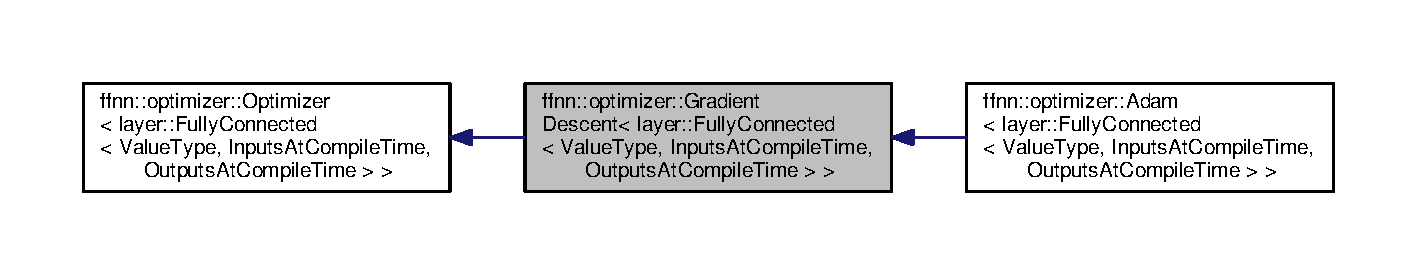
\includegraphics[width=350pt]{classffnn_1_1optimizer_1_1_gradient_descent_3_01layer_1_1_fully_connected_3_01_value_type_00_01_6ae520a76e559ae92ecb449366b20b6e}
\end{center}
\end{figure}


Collaboration diagram for ffnn\-:\-:optimizer\-:\-:Gradient\-Descent$<$ layer\-:\-:Fully\-Connected$<$ Value\-Type, Inputs\-At\-Compile\-Time, Outputs\-At\-Compile\-Time $>$ $>$\-:\nopagebreak
\begin{figure}[H]
\begin{center}
\leavevmode
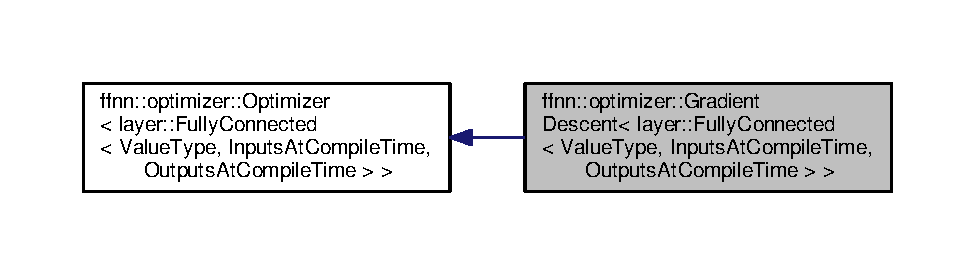
\includegraphics[width=350pt]{classffnn_1_1optimizer_1_1_gradient_descent_3_01layer_1_1_fully_connected_3_01_value_type_00_01_4afe58a57291e79801d5016d5e771823}
\end{center}
\end{figure}
\subsection*{Public Types}
\begin{DoxyCompactItemize}
\item 
typedef \hyperlink{classffnn_1_1layer_1_1_fully_connected}{layer\-::\-Fully\-Connected}\\*
$<$ Value\-Type, \\*
Inputs\-At\-Compile\-Time, \\*
Outputs\-At\-Compile\-Time $>$ \hyperlink{classffnn_1_1optimizer_1_1_gradient_descent_3_01layer_1_1_fully_connected_3_01_value_type_00_01_5f7b01db2ae4d39760d70ee323649a60_ad0c1e85b8917062542e3fdfceb41101d}{Layer\-Type}
\begin{DoxyCompactList}\small\item\em Layer type standardization. \end{DoxyCompactList}\item 
typedef Layer\-Type\-::\-Scalar \hyperlink{classffnn_1_1optimizer_1_1_gradient_descent_3_01layer_1_1_fully_connected_3_01_value_type_00_01_5f7b01db2ae4d39760d70ee323649a60_a6b0c0a8724609132c7bbbec6eb299181}{Scalar}
\begin{DoxyCompactList}\small\item\em Scalar type standardization. \end{DoxyCompactList}\item 
typedef Layer\-Type\-::\-Size\-Type \hyperlink{classffnn_1_1optimizer_1_1_gradient_descent_3_01layer_1_1_fully_connected_3_01_value_type_00_01_5f7b01db2ae4d39760d70ee323649a60_aefaefc86292acdb7d508c467102f7b19}{Size\-Type}
\begin{DoxyCompactList}\small\item\em Size type standardization. \end{DoxyCompactList}\item 
typedef Layer\-Type\-::\-Input\-Block\-Type \hyperlink{classffnn_1_1optimizer_1_1_gradient_descent_3_01layer_1_1_fully_connected_3_01_value_type_00_01_5f7b01db2ae4d39760d70ee323649a60_adf63a5c9be6baf42f54450549b809b73}{Input\-Block\-Type}
\begin{DoxyCompactList}\small\item\em Matrix type standardization. \end{DoxyCompactList}\item 
typedef Layer\-Type\-::\-Output\-Block\-Type \hyperlink{classffnn_1_1optimizer_1_1_gradient_descent_3_01layer_1_1_fully_connected_3_01_value_type_00_01_5f7b01db2ae4d39760d70ee323649a60_a656744c50766c58b1b094db14c2bfc44}{Output\-Block\-Type}
\begin{DoxyCompactList}\small\item\em Matrix type standardization. \end{DoxyCompactList}\item 
typedef Layer\-Type\-::\-Weight\-Matrix\-Type \hyperlink{classffnn_1_1optimizer_1_1_gradient_descent_3_01layer_1_1_fully_connected_3_01_value_type_00_01_5f7b01db2ae4d39760d70ee323649a60_a0d3b5fe84f944e4695a094f40f6a8bec}{Weight\-Matrix\-Type}
\begin{DoxyCompactList}\small\item\em Input-\/output weight matrix. \end{DoxyCompactList}\item 
typedef Layer\-Type\-::\-Bias\-Vector\-Type \hyperlink{classffnn_1_1optimizer_1_1_gradient_descent_3_01layer_1_1_fully_connected_3_01_value_type_00_01_5f7b01db2ae4d39760d70ee323649a60_aaca17a8f41752429974c4ba7e98bdb47}{Bias\-Vector\-Type}
\begin{DoxyCompactList}\small\item\em Bia vector type standardization. \end{DoxyCompactList}\end{DoxyCompactItemize}
\subsection*{Public Member Functions}
\begin{DoxyCompactItemize}
\item 
\hyperlink{classffnn_1_1optimizer_1_1_gradient_descent_3_01layer_1_1_fully_connected_3_01_value_type_00_01_5f7b01db2ae4d39760d70ee323649a60_afb880546a7d9bd01862278b6933728c7}{Gradient\-Descent} (\hyperlink{classffnn_1_1optimizer_1_1_gradient_descent_3_01layer_1_1_fully_connected_3_01_value_type_00_01_5f7b01db2ae4d39760d70ee323649a60_a6b0c0a8724609132c7bbbec6eb299181}{Scalar} lr)
\begin{DoxyCompactList}\small\item\em Setup constructor. \end{DoxyCompactList}\item 
virtual \hyperlink{classffnn_1_1optimizer_1_1_gradient_descent_3_01layer_1_1_fully_connected_3_01_value_type_00_01_5f7b01db2ae4d39760d70ee323649a60_a7e1f017295ef3e92e415691cc1495971}{$\sim$\-Gradient\-Descent} ()
\item 
virtual void \hyperlink{classffnn_1_1optimizer_1_1_gradient_descent_3_01layer_1_1_fully_connected_3_01_value_type_00_01_5f7b01db2ae4d39760d70ee323649a60_a2e152e94571b7948b514c9d4cbd70504}{initialize} (\hyperlink{classffnn_1_1optimizer_1_1_gradient_descent_3_01layer_1_1_fully_connected_3_01_value_type_00_01_5f7b01db2ae4d39760d70ee323649a60_ad0c1e85b8917062542e3fdfceb41101d}{Layer\-Type} \&layer)
\begin{DoxyCompactList}\small\item\em Initializes the \hyperlink{classffnn_1_1optimizer_1_1_optimizer}{Optimizer}. \end{DoxyCompactList}\item 
virtual void \hyperlink{classffnn_1_1optimizer_1_1_gradient_descent_3_01layer_1_1_fully_connected_3_01_value_type_00_01_5f7b01db2ae4d39760d70ee323649a60_a8317088f22bb86f204108a82f9233844}{reset} (\hyperlink{classffnn_1_1optimizer_1_1_gradient_descent_3_01layer_1_1_fully_connected_3_01_value_type_00_01_5f7b01db2ae4d39760d70ee323649a60_ad0c1e85b8917062542e3fdfceb41101d}{Layer\-Type} \&layer)
\begin{DoxyCompactList}\small\item\em Resetrs persistent \hyperlink{classffnn_1_1optimizer_1_1_optimizer}{Optimizer} states. \end{DoxyCompactList}\item 
virtual bool \hyperlink{classffnn_1_1optimizer_1_1_gradient_descent_3_01layer_1_1_fully_connected_3_01_value_type_00_01_5f7b01db2ae4d39760d70ee323649a60_afa8fe46160d16887fc7abb4de34a65e5}{forward} (\hyperlink{classffnn_1_1optimizer_1_1_gradient_descent_3_01layer_1_1_fully_connected_3_01_value_type_00_01_5f7b01db2ae4d39760d70ee323649a60_ad0c1e85b8917062542e3fdfceb41101d}{Layer\-Type} \&layer)
\begin{DoxyCompactList}\small\item\em Computes one forward optimization update step. \end{DoxyCompactList}\item 
virtual bool \hyperlink{classffnn_1_1optimizer_1_1_gradient_descent_3_01layer_1_1_fully_connected_3_01_value_type_00_01_5f7b01db2ae4d39760d70ee323649a60_a216318398f796e0b2a2522a45a4441be}{backward} (\hyperlink{classffnn_1_1optimizer_1_1_gradient_descent_3_01layer_1_1_fully_connected_3_01_value_type_00_01_5f7b01db2ae4d39760d70ee323649a60_ad0c1e85b8917062542e3fdfceb41101d}{Layer\-Type} \&layer)
\begin{DoxyCompactList}\small\item\em Computes optimization step during backward propogation. \end{DoxyCompactList}\item 
virtual bool \hyperlink{classffnn_1_1optimizer_1_1_gradient_descent_3_01layer_1_1_fully_connected_3_01_value_type_00_01_5f7b01db2ae4d39760d70ee323649a60_a4e15c26f4b561a8ea3ca3de3b324e1cf}{update} (\hyperlink{classffnn_1_1optimizer_1_1_gradient_descent_3_01layer_1_1_fully_connected_3_01_value_type_00_01_5f7b01db2ae4d39760d70ee323649a60_ad0c1e85b8917062542e3fdfceb41101d}{Layer\-Type} \&layer)
\begin{DoxyCompactList}\small\item\em Applies optimization update. \end{DoxyCompactList}\end{DoxyCompactItemize}
\subsection*{Protected Attributes}
\begin{DoxyCompactItemize}
\item 
\hyperlink{classffnn_1_1optimizer_1_1_gradient_descent_3_01layer_1_1_fully_connected_3_01_value_type_00_01_5f7b01db2ae4d39760d70ee323649a60_a6b0c0a8724609132c7bbbec6eb299181}{Scalar} \hyperlink{classffnn_1_1optimizer_1_1_gradient_descent_3_01layer_1_1_fully_connected_3_01_value_type_00_01_5f7b01db2ae4d39760d70ee323649a60_ae93f581c5257c180827d0dea59f64033}{lr\-\_\-}
\begin{DoxyCompactList}\small\item\em Learning rate. \end{DoxyCompactList}\item 
\hyperlink{classffnn_1_1optimizer_1_1_gradient_descent_3_01layer_1_1_fully_connected_3_01_value_type_00_01_5f7b01db2ae4d39760d70ee323649a60_a0d3b5fe84f944e4695a094f40f6a8bec}{Weight\-Matrix\-Type} \hyperlink{classffnn_1_1optimizer_1_1_gradient_descent_3_01layer_1_1_fully_connected_3_01_value_type_00_01_5f7b01db2ae4d39760d70ee323649a60_a3a3cad49f1855a20dbf9ff62178bf9ff}{weight\-\_\-gradient\-\_\-}
\begin{DoxyCompactList}\small\item\em Total weight matrix gradient. \end{DoxyCompactList}\item 
\hyperlink{classffnn_1_1optimizer_1_1_gradient_descent_3_01layer_1_1_fully_connected_3_01_value_type_00_01_5f7b01db2ae4d39760d70ee323649a60_aaca17a8f41752429974c4ba7e98bdb47}{Bias\-Vector\-Type} \hyperlink{classffnn_1_1optimizer_1_1_gradient_descent_3_01layer_1_1_fully_connected_3_01_value_type_00_01_5f7b01db2ae4d39760d70ee323649a60_ab9e5c3af9ed401ddc36ea6e2437e4e51}{bias\-\_\-gradient\-\_\-}
\begin{DoxyCompactList}\small\item\em Total bias vector delta. \end{DoxyCompactList}\item 
\hyperlink{classffnn_1_1optimizer_1_1_gradient_descent_3_01layer_1_1_fully_connected_3_01_value_type_00_01_5f7b01db2ae4d39760d70ee323649a60_adf63a5c9be6baf42f54450549b809b73}{Input\-Block\-Type} \hyperlink{classffnn_1_1optimizer_1_1_gradient_descent_3_01layer_1_1_fully_connected_3_01_value_type_00_01_5f7b01db2ae4d39760d70ee323649a60_a3f8d4e20a604d30d722a464f4e8c9523}{prev\-\_\-input\-\_\-}
\begin{DoxyCompactList}\small\item\em Previous input. \end{DoxyCompactList}\end{DoxyCompactItemize}


\subsection{Member Typedef Documentation}
\hypertarget{classffnn_1_1optimizer_1_1_gradient_descent_3_01layer_1_1_fully_connected_3_01_value_type_00_01_5f7b01db2ae4d39760d70ee323649a60_aaca17a8f41752429974c4ba7e98bdb47}{\index{ffnn\-::optimizer\-::\-Gradient\-Descent$<$ layer\-::\-Fully\-Connected$<$ Value\-Type, Inputs\-At\-Compile\-Time, Outputs\-At\-Compile\-Time $>$ $>$@{ffnn\-::optimizer\-::\-Gradient\-Descent$<$ layer\-::\-Fully\-Connected$<$ Value\-Type, Inputs\-At\-Compile\-Time, Outputs\-At\-Compile\-Time $>$ $>$}!Bias\-Vector\-Type@{Bias\-Vector\-Type}}
\index{Bias\-Vector\-Type@{Bias\-Vector\-Type}!ffnn::optimizer::GradientDescent< layer::FullyConnected< ValueType, InputsAtCompileTime, OutputsAtCompileTime > >@{ffnn\-::optimizer\-::\-Gradient\-Descent$<$ layer\-::\-Fully\-Connected$<$ Value\-Type, Inputs\-At\-Compile\-Time, Outputs\-At\-Compile\-Time $>$ $>$}}
\subsubsection[{Bias\-Vector\-Type}]{\setlength{\rightskip}{0pt plus 5cm}typedef Layer\-Type\-::\-Bias\-Vector\-Type {\bf ffnn\-::optimizer\-::\-Gradient\-Descent}$<$ {\bf layer\-::\-Fully\-Connected}$<$ Value\-Type, Inputs\-At\-Compile\-Time, Outputs\-At\-Compile\-Time $>$ $>$\-::{\bf Bias\-Vector\-Type}}}\label{classffnn_1_1optimizer_1_1_gradient_descent_3_01layer_1_1_fully_connected_3_01_value_type_00_01_5f7b01db2ae4d39760d70ee323649a60_aaca17a8f41752429974c4ba7e98bdb47}


Bia vector type standardization. 

\hypertarget{classffnn_1_1optimizer_1_1_gradient_descent_3_01layer_1_1_fully_connected_3_01_value_type_00_01_5f7b01db2ae4d39760d70ee323649a60_adf63a5c9be6baf42f54450549b809b73}{\index{ffnn\-::optimizer\-::\-Gradient\-Descent$<$ layer\-::\-Fully\-Connected$<$ Value\-Type, Inputs\-At\-Compile\-Time, Outputs\-At\-Compile\-Time $>$ $>$@{ffnn\-::optimizer\-::\-Gradient\-Descent$<$ layer\-::\-Fully\-Connected$<$ Value\-Type, Inputs\-At\-Compile\-Time, Outputs\-At\-Compile\-Time $>$ $>$}!Input\-Block\-Type@{Input\-Block\-Type}}
\index{Input\-Block\-Type@{Input\-Block\-Type}!ffnn::optimizer::GradientDescent< layer::FullyConnected< ValueType, InputsAtCompileTime, OutputsAtCompileTime > >@{ffnn\-::optimizer\-::\-Gradient\-Descent$<$ layer\-::\-Fully\-Connected$<$ Value\-Type, Inputs\-At\-Compile\-Time, Outputs\-At\-Compile\-Time $>$ $>$}}
\subsubsection[{Input\-Block\-Type}]{\setlength{\rightskip}{0pt plus 5cm}typedef Layer\-Type\-::\-Input\-Block\-Type {\bf ffnn\-::optimizer\-::\-Gradient\-Descent}$<$ {\bf layer\-::\-Fully\-Connected}$<$ Value\-Type, Inputs\-At\-Compile\-Time, Outputs\-At\-Compile\-Time $>$ $>$\-::{\bf Input\-Block\-Type}}}\label{classffnn_1_1optimizer_1_1_gradient_descent_3_01layer_1_1_fully_connected_3_01_value_type_00_01_5f7b01db2ae4d39760d70ee323649a60_adf63a5c9be6baf42f54450549b809b73}


Matrix type standardization. 

\hypertarget{classffnn_1_1optimizer_1_1_gradient_descent_3_01layer_1_1_fully_connected_3_01_value_type_00_01_5f7b01db2ae4d39760d70ee323649a60_ad0c1e85b8917062542e3fdfceb41101d}{\index{ffnn\-::optimizer\-::\-Gradient\-Descent$<$ layer\-::\-Fully\-Connected$<$ Value\-Type, Inputs\-At\-Compile\-Time, Outputs\-At\-Compile\-Time $>$ $>$@{ffnn\-::optimizer\-::\-Gradient\-Descent$<$ layer\-::\-Fully\-Connected$<$ Value\-Type, Inputs\-At\-Compile\-Time, Outputs\-At\-Compile\-Time $>$ $>$}!Layer\-Type@{Layer\-Type}}
\index{Layer\-Type@{Layer\-Type}!ffnn::optimizer::GradientDescent< layer::FullyConnected< ValueType, InputsAtCompileTime, OutputsAtCompileTime > >@{ffnn\-::optimizer\-::\-Gradient\-Descent$<$ layer\-::\-Fully\-Connected$<$ Value\-Type, Inputs\-At\-Compile\-Time, Outputs\-At\-Compile\-Time $>$ $>$}}
\subsubsection[{Layer\-Type}]{\setlength{\rightskip}{0pt plus 5cm}typedef {\bf layer\-::\-Fully\-Connected}$<$Value\-Type, Inputs\-At\-Compile\-Time, Outputs\-At\-Compile\-Time$>$ {\bf ffnn\-::optimizer\-::\-Gradient\-Descent}$<$ {\bf layer\-::\-Fully\-Connected}$<$ Value\-Type, Inputs\-At\-Compile\-Time, Outputs\-At\-Compile\-Time $>$ $>$\-::{\bf Layer\-Type}}}\label{classffnn_1_1optimizer_1_1_gradient_descent_3_01layer_1_1_fully_connected_3_01_value_type_00_01_5f7b01db2ae4d39760d70ee323649a60_ad0c1e85b8917062542e3fdfceb41101d}


Layer type standardization. 

\hypertarget{classffnn_1_1optimizer_1_1_gradient_descent_3_01layer_1_1_fully_connected_3_01_value_type_00_01_5f7b01db2ae4d39760d70ee323649a60_a656744c50766c58b1b094db14c2bfc44}{\index{ffnn\-::optimizer\-::\-Gradient\-Descent$<$ layer\-::\-Fully\-Connected$<$ Value\-Type, Inputs\-At\-Compile\-Time, Outputs\-At\-Compile\-Time $>$ $>$@{ffnn\-::optimizer\-::\-Gradient\-Descent$<$ layer\-::\-Fully\-Connected$<$ Value\-Type, Inputs\-At\-Compile\-Time, Outputs\-At\-Compile\-Time $>$ $>$}!Output\-Block\-Type@{Output\-Block\-Type}}
\index{Output\-Block\-Type@{Output\-Block\-Type}!ffnn::optimizer::GradientDescent< layer::FullyConnected< ValueType, InputsAtCompileTime, OutputsAtCompileTime > >@{ffnn\-::optimizer\-::\-Gradient\-Descent$<$ layer\-::\-Fully\-Connected$<$ Value\-Type, Inputs\-At\-Compile\-Time, Outputs\-At\-Compile\-Time $>$ $>$}}
\subsubsection[{Output\-Block\-Type}]{\setlength{\rightskip}{0pt plus 5cm}typedef Layer\-Type\-::\-Output\-Block\-Type {\bf ffnn\-::optimizer\-::\-Gradient\-Descent}$<$ {\bf layer\-::\-Fully\-Connected}$<$ Value\-Type, Inputs\-At\-Compile\-Time, Outputs\-At\-Compile\-Time $>$ $>$\-::{\bf Output\-Block\-Type}}}\label{classffnn_1_1optimizer_1_1_gradient_descent_3_01layer_1_1_fully_connected_3_01_value_type_00_01_5f7b01db2ae4d39760d70ee323649a60_a656744c50766c58b1b094db14c2bfc44}


Matrix type standardization. 

\hypertarget{classffnn_1_1optimizer_1_1_gradient_descent_3_01layer_1_1_fully_connected_3_01_value_type_00_01_5f7b01db2ae4d39760d70ee323649a60_a6b0c0a8724609132c7bbbec6eb299181}{\index{ffnn\-::optimizer\-::\-Gradient\-Descent$<$ layer\-::\-Fully\-Connected$<$ Value\-Type, Inputs\-At\-Compile\-Time, Outputs\-At\-Compile\-Time $>$ $>$@{ffnn\-::optimizer\-::\-Gradient\-Descent$<$ layer\-::\-Fully\-Connected$<$ Value\-Type, Inputs\-At\-Compile\-Time, Outputs\-At\-Compile\-Time $>$ $>$}!Scalar@{Scalar}}
\index{Scalar@{Scalar}!ffnn::optimizer::GradientDescent< layer::FullyConnected< ValueType, InputsAtCompileTime, OutputsAtCompileTime > >@{ffnn\-::optimizer\-::\-Gradient\-Descent$<$ layer\-::\-Fully\-Connected$<$ Value\-Type, Inputs\-At\-Compile\-Time, Outputs\-At\-Compile\-Time $>$ $>$}}
\subsubsection[{Scalar}]{\setlength{\rightskip}{0pt plus 5cm}typedef Layer\-Type\-::\-Scalar {\bf ffnn\-::optimizer\-::\-Gradient\-Descent}$<$ {\bf layer\-::\-Fully\-Connected}$<$ Value\-Type, Inputs\-At\-Compile\-Time, Outputs\-At\-Compile\-Time $>$ $>$\-::{\bf Scalar}}}\label{classffnn_1_1optimizer_1_1_gradient_descent_3_01layer_1_1_fully_connected_3_01_value_type_00_01_5f7b01db2ae4d39760d70ee323649a60_a6b0c0a8724609132c7bbbec6eb299181}


Scalar type standardization. 

\hypertarget{classffnn_1_1optimizer_1_1_gradient_descent_3_01layer_1_1_fully_connected_3_01_value_type_00_01_5f7b01db2ae4d39760d70ee323649a60_aefaefc86292acdb7d508c467102f7b19}{\index{ffnn\-::optimizer\-::\-Gradient\-Descent$<$ layer\-::\-Fully\-Connected$<$ Value\-Type, Inputs\-At\-Compile\-Time, Outputs\-At\-Compile\-Time $>$ $>$@{ffnn\-::optimizer\-::\-Gradient\-Descent$<$ layer\-::\-Fully\-Connected$<$ Value\-Type, Inputs\-At\-Compile\-Time, Outputs\-At\-Compile\-Time $>$ $>$}!Size\-Type@{Size\-Type}}
\index{Size\-Type@{Size\-Type}!ffnn::optimizer::GradientDescent< layer::FullyConnected< ValueType, InputsAtCompileTime, OutputsAtCompileTime > >@{ffnn\-::optimizer\-::\-Gradient\-Descent$<$ layer\-::\-Fully\-Connected$<$ Value\-Type, Inputs\-At\-Compile\-Time, Outputs\-At\-Compile\-Time $>$ $>$}}
\subsubsection[{Size\-Type}]{\setlength{\rightskip}{0pt plus 5cm}typedef Layer\-Type\-::\-Size\-Type {\bf ffnn\-::optimizer\-::\-Gradient\-Descent}$<$ {\bf layer\-::\-Fully\-Connected}$<$ Value\-Type, Inputs\-At\-Compile\-Time, Outputs\-At\-Compile\-Time $>$ $>$\-::{\bf Size\-Type}}}\label{classffnn_1_1optimizer_1_1_gradient_descent_3_01layer_1_1_fully_connected_3_01_value_type_00_01_5f7b01db2ae4d39760d70ee323649a60_aefaefc86292acdb7d508c467102f7b19}


Size type standardization. 

\hypertarget{classffnn_1_1optimizer_1_1_gradient_descent_3_01layer_1_1_fully_connected_3_01_value_type_00_01_5f7b01db2ae4d39760d70ee323649a60_a0d3b5fe84f944e4695a094f40f6a8bec}{\index{ffnn\-::optimizer\-::\-Gradient\-Descent$<$ layer\-::\-Fully\-Connected$<$ Value\-Type, Inputs\-At\-Compile\-Time, Outputs\-At\-Compile\-Time $>$ $>$@{ffnn\-::optimizer\-::\-Gradient\-Descent$<$ layer\-::\-Fully\-Connected$<$ Value\-Type, Inputs\-At\-Compile\-Time, Outputs\-At\-Compile\-Time $>$ $>$}!Weight\-Matrix\-Type@{Weight\-Matrix\-Type}}
\index{Weight\-Matrix\-Type@{Weight\-Matrix\-Type}!ffnn::optimizer::GradientDescent< layer::FullyConnected< ValueType, InputsAtCompileTime, OutputsAtCompileTime > >@{ffnn\-::optimizer\-::\-Gradient\-Descent$<$ layer\-::\-Fully\-Connected$<$ Value\-Type, Inputs\-At\-Compile\-Time, Outputs\-At\-Compile\-Time $>$ $>$}}
\subsubsection[{Weight\-Matrix\-Type}]{\setlength{\rightskip}{0pt plus 5cm}typedef Layer\-Type\-::\-Weight\-Matrix\-Type {\bf ffnn\-::optimizer\-::\-Gradient\-Descent}$<$ {\bf layer\-::\-Fully\-Connected}$<$ Value\-Type, Inputs\-At\-Compile\-Time, Outputs\-At\-Compile\-Time $>$ $>$\-::{\bf Weight\-Matrix\-Type}}}\label{classffnn_1_1optimizer_1_1_gradient_descent_3_01layer_1_1_fully_connected_3_01_value_type_00_01_5f7b01db2ae4d39760d70ee323649a60_a0d3b5fe84f944e4695a094f40f6a8bec}


Input-\/output weight matrix. 



\subsection{Constructor \& Destructor Documentation}
\hypertarget{classffnn_1_1optimizer_1_1_gradient_descent_3_01layer_1_1_fully_connected_3_01_value_type_00_01_5f7b01db2ae4d39760d70ee323649a60_afb880546a7d9bd01862278b6933728c7}{\index{ffnn\-::optimizer\-::\-Gradient\-Descent$<$ layer\-::\-Fully\-Connected$<$ Value\-Type, Inputs\-At\-Compile\-Time, Outputs\-At\-Compile\-Time $>$ $>$@{ffnn\-::optimizer\-::\-Gradient\-Descent$<$ layer\-::\-Fully\-Connected$<$ Value\-Type, Inputs\-At\-Compile\-Time, Outputs\-At\-Compile\-Time $>$ $>$}!Gradient\-Descent@{Gradient\-Descent}}
\index{Gradient\-Descent@{Gradient\-Descent}!ffnn::optimizer::GradientDescent< layer::FullyConnected< ValueType, InputsAtCompileTime, OutputsAtCompileTime > >@{ffnn\-::optimizer\-::\-Gradient\-Descent$<$ layer\-::\-Fully\-Connected$<$ Value\-Type, Inputs\-At\-Compile\-Time, Outputs\-At\-Compile\-Time $>$ $>$}}
\subsubsection[{Gradient\-Descent}]{\setlength{\rightskip}{0pt plus 5cm}{\bf ffnn\-::optimizer\-::\-Gradient\-Descent}$<$ {\bf layer\-::\-Fully\-Connected}$<$ Value\-Type, Inputs\-At\-Compile\-Time, Outputs\-At\-Compile\-Time $>$ $>$\-::{\bf Gradient\-Descent} (
\begin{DoxyParamCaption}
\item[{{\bf Scalar}}]{lr}
\end{DoxyParamCaption}
)\hspace{0.3cm}{\ttfamily [inline]}, {\ttfamily [explicit]}}}\label{classffnn_1_1optimizer_1_1_gradient_descent_3_01layer_1_1_fully_connected_3_01_value_type_00_01_5f7b01db2ae4d39760d70ee323649a60_afb880546a7d9bd01862278b6933728c7}


Setup constructor. 


\begin{DoxyParams}{Parameters}
{\em lr} & Learning rate \\
\hline
\end{DoxyParams}
\hypertarget{classffnn_1_1optimizer_1_1_gradient_descent_3_01layer_1_1_fully_connected_3_01_value_type_00_01_5f7b01db2ae4d39760d70ee323649a60_a7e1f017295ef3e92e415691cc1495971}{\index{ffnn\-::optimizer\-::\-Gradient\-Descent$<$ layer\-::\-Fully\-Connected$<$ Value\-Type, Inputs\-At\-Compile\-Time, Outputs\-At\-Compile\-Time $>$ $>$@{ffnn\-::optimizer\-::\-Gradient\-Descent$<$ layer\-::\-Fully\-Connected$<$ Value\-Type, Inputs\-At\-Compile\-Time, Outputs\-At\-Compile\-Time $>$ $>$}!$\sim$\-Gradient\-Descent@{$\sim$\-Gradient\-Descent}}
\index{$\sim$\-Gradient\-Descent@{$\sim$\-Gradient\-Descent}!ffnn::optimizer::GradientDescent< layer::FullyConnected< ValueType, InputsAtCompileTime, OutputsAtCompileTime > >@{ffnn\-::optimizer\-::\-Gradient\-Descent$<$ layer\-::\-Fully\-Connected$<$ Value\-Type, Inputs\-At\-Compile\-Time, Outputs\-At\-Compile\-Time $>$ $>$}}
\subsubsection[{$\sim$\-Gradient\-Descent}]{\setlength{\rightskip}{0pt plus 5cm}virtual {\bf ffnn\-::optimizer\-::\-Gradient\-Descent}$<$ {\bf layer\-::\-Fully\-Connected}$<$ Value\-Type, Inputs\-At\-Compile\-Time, Outputs\-At\-Compile\-Time $>$ $>$\-::$\sim${\bf Gradient\-Descent} (
\begin{DoxyParamCaption}
{}
\end{DoxyParamCaption}
)\hspace{0.3cm}{\ttfamily [inline]}, {\ttfamily [virtual]}}}\label{classffnn_1_1optimizer_1_1_gradient_descent_3_01layer_1_1_fully_connected_3_01_value_type_00_01_5f7b01db2ae4d39760d70ee323649a60_a7e1f017295ef3e92e415691cc1495971}


\subsection{Member Function Documentation}
\hypertarget{classffnn_1_1optimizer_1_1_gradient_descent_3_01layer_1_1_fully_connected_3_01_value_type_00_01_5f7b01db2ae4d39760d70ee323649a60_a216318398f796e0b2a2522a45a4441be}{\index{ffnn\-::optimizer\-::\-Gradient\-Descent$<$ layer\-::\-Fully\-Connected$<$ Value\-Type, Inputs\-At\-Compile\-Time, Outputs\-At\-Compile\-Time $>$ $>$@{ffnn\-::optimizer\-::\-Gradient\-Descent$<$ layer\-::\-Fully\-Connected$<$ Value\-Type, Inputs\-At\-Compile\-Time, Outputs\-At\-Compile\-Time $>$ $>$}!backward@{backward}}
\index{backward@{backward}!ffnn::optimizer::GradientDescent< layer::FullyConnected< ValueType, InputsAtCompileTime, OutputsAtCompileTime > >@{ffnn\-::optimizer\-::\-Gradient\-Descent$<$ layer\-::\-Fully\-Connected$<$ Value\-Type, Inputs\-At\-Compile\-Time, Outputs\-At\-Compile\-Time $>$ $>$}}
\subsubsection[{backward}]{\setlength{\rightskip}{0pt plus 5cm}virtual bool {\bf ffnn\-::optimizer\-::\-Gradient\-Descent}$<$ {\bf layer\-::\-Fully\-Connected}$<$ Value\-Type, Inputs\-At\-Compile\-Time, Outputs\-At\-Compile\-Time $>$ $>$\-::backward (
\begin{DoxyParamCaption}
\item[{{\bf Layer\-Type} \&}]{layer}
\end{DoxyParamCaption}
)\hspace{0.3cm}{\ttfamily [inline]}, {\ttfamily [virtual]}}}\label{classffnn_1_1optimizer_1_1_gradient_descent_3_01layer_1_1_fully_connected_3_01_value_type_00_01_5f7b01db2ae4d39760d70ee323649a60_a216318398f796e0b2a2522a45a4441be}


Computes optimization step during backward propogation. 


\begin{DoxyParams}[1]{Parameters}
\mbox{\tt in,out}  & {\em layer} & Layer to optimize \\
\hline
\end{DoxyParams}

\begin{DoxyRetVals}{Return values}
{\em true} & if optimization setp was successful \\
\hline
{\em false} & otherwise \\
\hline
\end{DoxyRetVals}


Implements \hyperlink{classffnn_1_1optimizer_1_1_optimizer_ab1f9b1cae01f93f53ecf7119bedb6369}{ffnn\-::optimizer\-::\-Optimizer$<$ layer\-::\-Fully\-Connected$<$ Value\-Type, Inputs\-At\-Compile\-Time, Outputs\-At\-Compile\-Time $>$ $>$}.

\hypertarget{classffnn_1_1optimizer_1_1_gradient_descent_3_01layer_1_1_fully_connected_3_01_value_type_00_01_5f7b01db2ae4d39760d70ee323649a60_afa8fe46160d16887fc7abb4de34a65e5}{\index{ffnn\-::optimizer\-::\-Gradient\-Descent$<$ layer\-::\-Fully\-Connected$<$ Value\-Type, Inputs\-At\-Compile\-Time, Outputs\-At\-Compile\-Time $>$ $>$@{ffnn\-::optimizer\-::\-Gradient\-Descent$<$ layer\-::\-Fully\-Connected$<$ Value\-Type, Inputs\-At\-Compile\-Time, Outputs\-At\-Compile\-Time $>$ $>$}!forward@{forward}}
\index{forward@{forward}!ffnn::optimizer::GradientDescent< layer::FullyConnected< ValueType, InputsAtCompileTime, OutputsAtCompileTime > >@{ffnn\-::optimizer\-::\-Gradient\-Descent$<$ layer\-::\-Fully\-Connected$<$ Value\-Type, Inputs\-At\-Compile\-Time, Outputs\-At\-Compile\-Time $>$ $>$}}
\subsubsection[{forward}]{\setlength{\rightskip}{0pt plus 5cm}virtual bool {\bf ffnn\-::optimizer\-::\-Gradient\-Descent}$<$ {\bf layer\-::\-Fully\-Connected}$<$ Value\-Type, Inputs\-At\-Compile\-Time, Outputs\-At\-Compile\-Time $>$ $>$\-::forward (
\begin{DoxyParamCaption}
\item[{{\bf Layer\-Type} \&}]{layer}
\end{DoxyParamCaption}
)\hspace{0.3cm}{\ttfamily [inline]}, {\ttfamily [virtual]}}}\label{classffnn_1_1optimizer_1_1_gradient_descent_3_01layer_1_1_fully_connected_3_01_value_type_00_01_5f7b01db2ae4d39760d70ee323649a60_afa8fe46160d16887fc7abb4de34a65e5}


Computes one forward optimization update step. 


\begin{DoxyParams}[1]{Parameters}
\mbox{\tt in,out}  & {\em layer} & Layer to optimize \\
\hline
\end{DoxyParams}

\begin{DoxyRetVals}{Return values}
{\em true} & if optimization setp was successful \\
\hline
{\em false} & otherwise \\
\hline
\end{DoxyRetVals}


Implements \hyperlink{classffnn_1_1optimizer_1_1_optimizer_a80505cfdeba0a3c8d1db19a2821613f2}{ffnn\-::optimizer\-::\-Optimizer$<$ layer\-::\-Fully\-Connected$<$ Value\-Type, Inputs\-At\-Compile\-Time, Outputs\-At\-Compile\-Time $>$ $>$}.

\hypertarget{classffnn_1_1optimizer_1_1_gradient_descent_3_01layer_1_1_fully_connected_3_01_value_type_00_01_5f7b01db2ae4d39760d70ee323649a60_a2e152e94571b7948b514c9d4cbd70504}{\index{ffnn\-::optimizer\-::\-Gradient\-Descent$<$ layer\-::\-Fully\-Connected$<$ Value\-Type, Inputs\-At\-Compile\-Time, Outputs\-At\-Compile\-Time $>$ $>$@{ffnn\-::optimizer\-::\-Gradient\-Descent$<$ layer\-::\-Fully\-Connected$<$ Value\-Type, Inputs\-At\-Compile\-Time, Outputs\-At\-Compile\-Time $>$ $>$}!initialize@{initialize}}
\index{initialize@{initialize}!ffnn::optimizer::GradientDescent< layer::FullyConnected< ValueType, InputsAtCompileTime, OutputsAtCompileTime > >@{ffnn\-::optimizer\-::\-Gradient\-Descent$<$ layer\-::\-Fully\-Connected$<$ Value\-Type, Inputs\-At\-Compile\-Time, Outputs\-At\-Compile\-Time $>$ $>$}}
\subsubsection[{initialize}]{\setlength{\rightskip}{0pt plus 5cm}virtual void {\bf ffnn\-::optimizer\-::\-Gradient\-Descent}$<$ {\bf layer\-::\-Fully\-Connected}$<$ Value\-Type, Inputs\-At\-Compile\-Time, Outputs\-At\-Compile\-Time $>$ $>$\-::initialize (
\begin{DoxyParamCaption}
\item[{{\bf Layer\-Type} \&}]{layer}
\end{DoxyParamCaption}
)\hspace{0.3cm}{\ttfamily [inline]}, {\ttfamily [virtual]}}}\label{classffnn_1_1optimizer_1_1_gradient_descent_3_01layer_1_1_fully_connected_3_01_value_type_00_01_5f7b01db2ae4d39760d70ee323649a60_a2e152e94571b7948b514c9d4cbd70504}


Initializes the \hyperlink{classffnn_1_1optimizer_1_1_optimizer}{Optimizer}. 


\begin{DoxyParams}[1]{Parameters}
\mbox{\tt in,out}  & {\em layer} & Layer to optimize \\
\hline
\end{DoxyParams}


Implements \hyperlink{classffnn_1_1optimizer_1_1_optimizer_a4302b66ba9b013ae4833eca235ff306a}{ffnn\-::optimizer\-::\-Optimizer$<$ layer\-::\-Fully\-Connected$<$ Value\-Type, Inputs\-At\-Compile\-Time, Outputs\-At\-Compile\-Time $>$ $>$}.



Reimplemented in \hyperlink{classffnn_1_1optimizer_1_1_adam_3_01layer_1_1_fully_connected_3_01_value_type_00_01_inputs_at_co08ce471fd3ee7441a350cc42cfd35bcd_aa67f949f7a1228c221d06b1b1e03c28b}{ffnn\-::optimizer\-::\-Adam$<$ layer\-::\-Fully\-Connected$<$ Value\-Type, Inputs\-At\-Compile\-Time, Outputs\-At\-Compile\-Time $>$ $>$}.

\hypertarget{classffnn_1_1optimizer_1_1_gradient_descent_3_01layer_1_1_fully_connected_3_01_value_type_00_01_5f7b01db2ae4d39760d70ee323649a60_a8317088f22bb86f204108a82f9233844}{\index{ffnn\-::optimizer\-::\-Gradient\-Descent$<$ layer\-::\-Fully\-Connected$<$ Value\-Type, Inputs\-At\-Compile\-Time, Outputs\-At\-Compile\-Time $>$ $>$@{ffnn\-::optimizer\-::\-Gradient\-Descent$<$ layer\-::\-Fully\-Connected$<$ Value\-Type, Inputs\-At\-Compile\-Time, Outputs\-At\-Compile\-Time $>$ $>$}!reset@{reset}}
\index{reset@{reset}!ffnn::optimizer::GradientDescent< layer::FullyConnected< ValueType, InputsAtCompileTime, OutputsAtCompileTime > >@{ffnn\-::optimizer\-::\-Gradient\-Descent$<$ layer\-::\-Fully\-Connected$<$ Value\-Type, Inputs\-At\-Compile\-Time, Outputs\-At\-Compile\-Time $>$ $>$}}
\subsubsection[{reset}]{\setlength{\rightskip}{0pt plus 5cm}virtual void {\bf ffnn\-::optimizer\-::\-Gradient\-Descent}$<$ {\bf layer\-::\-Fully\-Connected}$<$ Value\-Type, Inputs\-At\-Compile\-Time, Outputs\-At\-Compile\-Time $>$ $>$\-::reset (
\begin{DoxyParamCaption}
\item[{{\bf Layer\-Type} \&}]{layer}
\end{DoxyParamCaption}
)\hspace{0.3cm}{\ttfamily [inline]}, {\ttfamily [virtual]}}}\label{classffnn_1_1optimizer_1_1_gradient_descent_3_01layer_1_1_fully_connected_3_01_value_type_00_01_5f7b01db2ae4d39760d70ee323649a60_a8317088f22bb86f204108a82f9233844}


Resetrs persistent \hyperlink{classffnn_1_1optimizer_1_1_optimizer}{Optimizer} states. 


\begin{DoxyParams}[1]{Parameters}
\mbox{\tt in,out}  & {\em layer} & Layer to optimize \\
\hline
\end{DoxyParams}


Implements \hyperlink{classffnn_1_1optimizer_1_1_optimizer_ade04e7582eb7b833713a9bd33e0e8346}{ffnn\-::optimizer\-::\-Optimizer$<$ layer\-::\-Fully\-Connected$<$ Value\-Type, Inputs\-At\-Compile\-Time, Outputs\-At\-Compile\-Time $>$ $>$}.

\hypertarget{classffnn_1_1optimizer_1_1_gradient_descent_3_01layer_1_1_fully_connected_3_01_value_type_00_01_5f7b01db2ae4d39760d70ee323649a60_a4e15c26f4b561a8ea3ca3de3b324e1cf}{\index{ffnn\-::optimizer\-::\-Gradient\-Descent$<$ layer\-::\-Fully\-Connected$<$ Value\-Type, Inputs\-At\-Compile\-Time, Outputs\-At\-Compile\-Time $>$ $>$@{ffnn\-::optimizer\-::\-Gradient\-Descent$<$ layer\-::\-Fully\-Connected$<$ Value\-Type, Inputs\-At\-Compile\-Time, Outputs\-At\-Compile\-Time $>$ $>$}!update@{update}}
\index{update@{update}!ffnn::optimizer::GradientDescent< layer::FullyConnected< ValueType, InputsAtCompileTime, OutputsAtCompileTime > >@{ffnn\-::optimizer\-::\-Gradient\-Descent$<$ layer\-::\-Fully\-Connected$<$ Value\-Type, Inputs\-At\-Compile\-Time, Outputs\-At\-Compile\-Time $>$ $>$}}
\subsubsection[{update}]{\setlength{\rightskip}{0pt plus 5cm}virtual bool {\bf ffnn\-::optimizer\-::\-Gradient\-Descent}$<$ {\bf layer\-::\-Fully\-Connected}$<$ Value\-Type, Inputs\-At\-Compile\-Time, Outputs\-At\-Compile\-Time $>$ $>$\-::update (
\begin{DoxyParamCaption}
\item[{{\bf Layer\-Type} \&}]{layer}
\end{DoxyParamCaption}
)\hspace{0.3cm}{\ttfamily [inline]}, {\ttfamily [virtual]}}}\label{classffnn_1_1optimizer_1_1_gradient_descent_3_01layer_1_1_fully_connected_3_01_value_type_00_01_5f7b01db2ae4d39760d70ee323649a60_a4e15c26f4b561a8ea3ca3de3b324e1cf}


Applies optimization update. 


\begin{DoxyParams}[1]{Parameters}
\mbox{\tt in,out}  & {\em layer} & Layer to optimize \\
\hline
\end{DoxyParams}

\begin{DoxyRetVals}{Return values}
{\em true} & if optimization update was applied successfully \\
\hline
{\em false} & otherwise \\
\hline
\end{DoxyRetVals}


Implements \hyperlink{classffnn_1_1optimizer_1_1_optimizer_a7c88c2794446e03ccd41628bb25d7a07}{ffnn\-::optimizer\-::\-Optimizer$<$ layer\-::\-Fully\-Connected$<$ Value\-Type, Inputs\-At\-Compile\-Time, Outputs\-At\-Compile\-Time $>$ $>$}.



Reimplemented in \hyperlink{classffnn_1_1optimizer_1_1_adam_3_01layer_1_1_fully_connected_3_01_value_type_00_01_inputs_at_co08ce471fd3ee7441a350cc42cfd35bcd_ad42586e39195fc9a72057f20b657f8be}{ffnn\-::optimizer\-::\-Adam$<$ layer\-::\-Fully\-Connected$<$ Value\-Type, Inputs\-At\-Compile\-Time, Outputs\-At\-Compile\-Time $>$ $>$}.



\subsection{Member Data Documentation}
\hypertarget{classffnn_1_1optimizer_1_1_gradient_descent_3_01layer_1_1_fully_connected_3_01_value_type_00_01_5f7b01db2ae4d39760d70ee323649a60_ab9e5c3af9ed401ddc36ea6e2437e4e51}{\index{ffnn\-::optimizer\-::\-Gradient\-Descent$<$ layer\-::\-Fully\-Connected$<$ Value\-Type, Inputs\-At\-Compile\-Time, Outputs\-At\-Compile\-Time $>$ $>$@{ffnn\-::optimizer\-::\-Gradient\-Descent$<$ layer\-::\-Fully\-Connected$<$ Value\-Type, Inputs\-At\-Compile\-Time, Outputs\-At\-Compile\-Time $>$ $>$}!bias\-\_\-gradient\-\_\-@{bias\-\_\-gradient\-\_\-}}
\index{bias\-\_\-gradient\-\_\-@{bias\-\_\-gradient\-\_\-}!ffnn::optimizer::GradientDescent< layer::FullyConnected< ValueType, InputsAtCompileTime, OutputsAtCompileTime > >@{ffnn\-::optimizer\-::\-Gradient\-Descent$<$ layer\-::\-Fully\-Connected$<$ Value\-Type, Inputs\-At\-Compile\-Time, Outputs\-At\-Compile\-Time $>$ $>$}}
\subsubsection[{bias\-\_\-gradient\-\_\-}]{\setlength{\rightskip}{0pt plus 5cm}{\bf Bias\-Vector\-Type} {\bf ffnn\-::optimizer\-::\-Gradient\-Descent}$<$ {\bf layer\-::\-Fully\-Connected}$<$ Value\-Type, Inputs\-At\-Compile\-Time, Outputs\-At\-Compile\-Time $>$ $>$\-::bias\-\_\-gradient\-\_\-\hspace{0.3cm}{\ttfamily [protected]}}}\label{classffnn_1_1optimizer_1_1_gradient_descent_3_01layer_1_1_fully_connected_3_01_value_type_00_01_5f7b01db2ae4d39760d70ee323649a60_ab9e5c3af9ed401ddc36ea6e2437e4e51}


Total bias vector delta. 

\hypertarget{classffnn_1_1optimizer_1_1_gradient_descent_3_01layer_1_1_fully_connected_3_01_value_type_00_01_5f7b01db2ae4d39760d70ee323649a60_ae93f581c5257c180827d0dea59f64033}{\index{ffnn\-::optimizer\-::\-Gradient\-Descent$<$ layer\-::\-Fully\-Connected$<$ Value\-Type, Inputs\-At\-Compile\-Time, Outputs\-At\-Compile\-Time $>$ $>$@{ffnn\-::optimizer\-::\-Gradient\-Descent$<$ layer\-::\-Fully\-Connected$<$ Value\-Type, Inputs\-At\-Compile\-Time, Outputs\-At\-Compile\-Time $>$ $>$}!lr\-\_\-@{lr\-\_\-}}
\index{lr\-\_\-@{lr\-\_\-}!ffnn::optimizer::GradientDescent< layer::FullyConnected< ValueType, InputsAtCompileTime, OutputsAtCompileTime > >@{ffnn\-::optimizer\-::\-Gradient\-Descent$<$ layer\-::\-Fully\-Connected$<$ Value\-Type, Inputs\-At\-Compile\-Time, Outputs\-At\-Compile\-Time $>$ $>$}}
\subsubsection[{lr\-\_\-}]{\setlength{\rightskip}{0pt plus 5cm}{\bf Scalar} {\bf ffnn\-::optimizer\-::\-Gradient\-Descent}$<$ {\bf layer\-::\-Fully\-Connected}$<$ Value\-Type, Inputs\-At\-Compile\-Time, Outputs\-At\-Compile\-Time $>$ $>$\-::lr\-\_\-\hspace{0.3cm}{\ttfamily [protected]}}}\label{classffnn_1_1optimizer_1_1_gradient_descent_3_01layer_1_1_fully_connected_3_01_value_type_00_01_5f7b01db2ae4d39760d70ee323649a60_ae93f581c5257c180827d0dea59f64033}


Learning rate. 

\hypertarget{classffnn_1_1optimizer_1_1_gradient_descent_3_01layer_1_1_fully_connected_3_01_value_type_00_01_5f7b01db2ae4d39760d70ee323649a60_a3f8d4e20a604d30d722a464f4e8c9523}{\index{ffnn\-::optimizer\-::\-Gradient\-Descent$<$ layer\-::\-Fully\-Connected$<$ Value\-Type, Inputs\-At\-Compile\-Time, Outputs\-At\-Compile\-Time $>$ $>$@{ffnn\-::optimizer\-::\-Gradient\-Descent$<$ layer\-::\-Fully\-Connected$<$ Value\-Type, Inputs\-At\-Compile\-Time, Outputs\-At\-Compile\-Time $>$ $>$}!prev\-\_\-input\-\_\-@{prev\-\_\-input\-\_\-}}
\index{prev\-\_\-input\-\_\-@{prev\-\_\-input\-\_\-}!ffnn::optimizer::GradientDescent< layer::FullyConnected< ValueType, InputsAtCompileTime, OutputsAtCompileTime > >@{ffnn\-::optimizer\-::\-Gradient\-Descent$<$ layer\-::\-Fully\-Connected$<$ Value\-Type, Inputs\-At\-Compile\-Time, Outputs\-At\-Compile\-Time $>$ $>$}}
\subsubsection[{prev\-\_\-input\-\_\-}]{\setlength{\rightskip}{0pt plus 5cm}{\bf Input\-Block\-Type} {\bf ffnn\-::optimizer\-::\-Gradient\-Descent}$<$ {\bf layer\-::\-Fully\-Connected}$<$ Value\-Type, Inputs\-At\-Compile\-Time, Outputs\-At\-Compile\-Time $>$ $>$\-::prev\-\_\-input\-\_\-\hspace{0.3cm}{\ttfamily [protected]}}}\label{classffnn_1_1optimizer_1_1_gradient_descent_3_01layer_1_1_fully_connected_3_01_value_type_00_01_5f7b01db2ae4d39760d70ee323649a60_a3f8d4e20a604d30d722a464f4e8c9523}


Previous input. 

\hypertarget{classffnn_1_1optimizer_1_1_gradient_descent_3_01layer_1_1_fully_connected_3_01_value_type_00_01_5f7b01db2ae4d39760d70ee323649a60_a3a3cad49f1855a20dbf9ff62178bf9ff}{\index{ffnn\-::optimizer\-::\-Gradient\-Descent$<$ layer\-::\-Fully\-Connected$<$ Value\-Type, Inputs\-At\-Compile\-Time, Outputs\-At\-Compile\-Time $>$ $>$@{ffnn\-::optimizer\-::\-Gradient\-Descent$<$ layer\-::\-Fully\-Connected$<$ Value\-Type, Inputs\-At\-Compile\-Time, Outputs\-At\-Compile\-Time $>$ $>$}!weight\-\_\-gradient\-\_\-@{weight\-\_\-gradient\-\_\-}}
\index{weight\-\_\-gradient\-\_\-@{weight\-\_\-gradient\-\_\-}!ffnn::optimizer::GradientDescent< layer::FullyConnected< ValueType, InputsAtCompileTime, OutputsAtCompileTime > >@{ffnn\-::optimizer\-::\-Gradient\-Descent$<$ layer\-::\-Fully\-Connected$<$ Value\-Type, Inputs\-At\-Compile\-Time, Outputs\-At\-Compile\-Time $>$ $>$}}
\subsubsection[{weight\-\_\-gradient\-\_\-}]{\setlength{\rightskip}{0pt plus 5cm}{\bf Weight\-Matrix\-Type} {\bf ffnn\-::optimizer\-::\-Gradient\-Descent}$<$ {\bf layer\-::\-Fully\-Connected}$<$ Value\-Type, Inputs\-At\-Compile\-Time, Outputs\-At\-Compile\-Time $>$ $>$\-::weight\-\_\-gradient\-\_\-\hspace{0.3cm}{\ttfamily [protected]}}}\label{classffnn_1_1optimizer_1_1_gradient_descent_3_01layer_1_1_fully_connected_3_01_value_type_00_01_5f7b01db2ae4d39760d70ee323649a60_a3a3cad49f1855a20dbf9ff62178bf9ff}


Total weight matrix gradient. 



The documentation for this class was generated from the following file\-:\begin{DoxyCompactItemize}
\item 
/home/briancairl/packages/src/ffnn-\/cpp/ffnn/include/ffnn/optimizer/impl/gradient\-\_\-descent/\hyperlink{optimizer_2impl_2gradient__descent_2fully__connected_8hpp}{fully\-\_\-connected.\-hpp}\end{DoxyCompactItemize}

\hypertarget{classffnn_1_1optimizer_1_1_gradient_descent_3_01layer_1_1_local_convolution_3_01_t_a_r_g_s_01_4_01_4}{\section{ffnn\-:\-:optimizer\-:\-:Gradient\-Descent$<$ layer\-:\-:Local\-Convolution$<$ T\-A\-R\-G\-S $>$ $>$ Class Template Reference}
\label{classffnn_1_1optimizer_1_1_gradient_descent_3_01layer_1_1_local_convolution_3_01_t_a_r_g_s_01_4_01_4}\index{ffnn\-::optimizer\-::\-Gradient\-Descent$<$ layer\-::\-Local\-Convolution$<$ T\-A\-R\-G\-S $>$ $>$@{ffnn\-::optimizer\-::\-Gradient\-Descent$<$ layer\-::\-Local\-Convolution$<$ T\-A\-R\-G\-S $>$ $>$}}
}


{\ttfamily \#include \char`\"{}local\-\_\-convolution.\-hpp\char`\"{}}



Inheritance diagram for ffnn\-:\-:optimizer\-:\-:Gradient\-Descent$<$ layer\-:\-:Local\-Convolution$<$ T\-A\-R\-G\-S $>$ $>$\-:\nopagebreak
\begin{figure}[H]
\begin{center}
\leavevmode
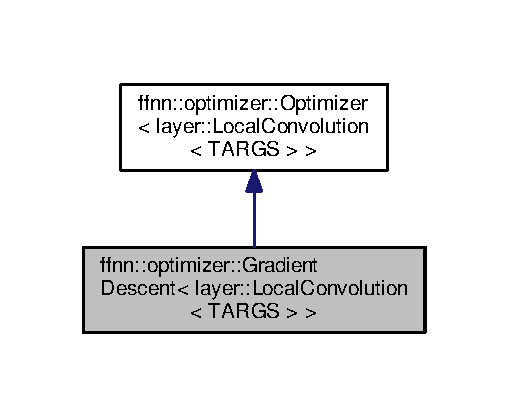
\includegraphics[width=244pt]{classffnn_1_1optimizer_1_1_gradient_descent_3_01layer_1_1_local_convolution_3_01_t_a_r_g_s_01_4_01_4__inherit__graph}
\end{center}
\end{figure}


Collaboration diagram for ffnn\-:\-:optimizer\-:\-:Gradient\-Descent$<$ layer\-:\-:Local\-Convolution$<$ T\-A\-R\-G\-S $>$ $>$\-:\nopagebreak
\begin{figure}[H]
\begin{center}
\leavevmode
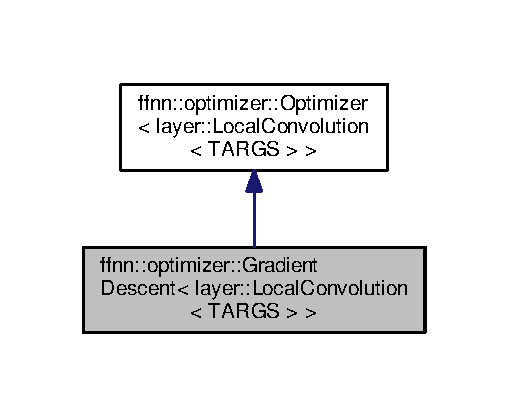
\includegraphics[width=244pt]{classffnn_1_1optimizer_1_1_gradient_descent_3_01layer_1_1_local_convolution_3_01_t_a_r_g_s_01_4_01_4__coll__graph}
\end{center}
\end{figure}
\subsection*{Public Types}
\begin{DoxyCompactItemize}
\item 
typedef \\*
layer\-::\-Local\-Convolution$<$ \hyperlink{local__convolution_8hpp_a005b9b79411aa786124330e813a99057}{T\-A\-R\-G\-S} $>$ \hyperlink{classffnn_1_1optimizer_1_1_gradient_descent_3_01layer_1_1_local_convolution_3_01_t_a_r_g_s_01_4_01_4_a16ba9a242dbe61604f16ff2ae19a4d1f}{Layer\-Type}
\begin{DoxyCompactList}\small\item\em Layer type standardization. \end{DoxyCompactList}\item 
typedef Layer\-Type\-::\-Scalar\-Type \hyperlink{classffnn_1_1optimizer_1_1_gradient_descent_3_01layer_1_1_local_convolution_3_01_t_a_r_g_s_01_4_01_4_ac3250ac9d0d3a0529a7e18a00f00233f}{Scalar\-Type}
\begin{DoxyCompactList}\small\item\em Scalar type standardization. \end{DoxyCompactList}\item 
typedef Layer\-Type\-::\-Size\-Type \hyperlink{classffnn_1_1optimizer_1_1_gradient_descent_3_01layer_1_1_local_convolution_3_01_t_a_r_g_s_01_4_01_4_a710d6fff7052b3fc2f032ca74b0c3026}{Size\-Type}
\begin{DoxyCompactList}\small\item\em Size type standardization. \end{DoxyCompactList}\item 
typedef Layer\-Type\-::\-Offset\-Type \hyperlink{classffnn_1_1optimizer_1_1_gradient_descent_3_01layer_1_1_local_convolution_3_01_t_a_r_g_s_01_4_01_4_aef03166f60cff06f14ed5e36cf371a5e}{Offset\-Type}
\begin{DoxyCompactList}\small\item\em Offset type standardization. \end{DoxyCompactList}\item 
typedef Layer\-Type\-::\-Input\-Block\-Type \hyperlink{classffnn_1_1optimizer_1_1_gradient_descent_3_01layer_1_1_local_convolution_3_01_t_a_r_g_s_01_4_01_4_af401944b8f1e2b6ed6cea8b8211e25f7}{Input\-Block\-Type}
\begin{DoxyCompactList}\small\item\em Matrix type standardization. \end{DoxyCompactList}\item 
typedef Layer\-Type\-::\-Output\-Block\-Type \hyperlink{classffnn_1_1optimizer_1_1_gradient_descent_3_01layer_1_1_local_convolution_3_01_t_a_r_g_s_01_4_01_4_aa20bbed306ab91d1e49da41491764c11}{Output\-Block\-Type}
\begin{DoxyCompactList}\small\item\em Matrix type standardization. \end{DoxyCompactList}\item 
typedef \\*
Layer\-Type\-::\-Parameter\-Block\-Type \hyperlink{classffnn_1_1optimizer_1_1_gradient_descent_3_01layer_1_1_local_convolution_3_01_t_a_r_g_s_01_4_01_4_aa3cf2a9b7dd4078926511651277aa953}{Parameter\-Block\-Type}
\begin{DoxyCompactList}\small\item\em Receptive-\/volume type standardization. \end{DoxyCompactList}\item 
typedef Layer\-Type\-::\-Parameters\-Type \hyperlink{classffnn_1_1optimizer_1_1_gradient_descent_3_01layer_1_1_local_convolution_3_01_t_a_r_g_s_01_4_01_4_ac7acd851ffa7a846dc07b2ef46a265ec}{Parameters\-Type}
\begin{DoxyCompactList}\small\item\em Receptive-\/field type standardization. \end{DoxyCompactList}\end{DoxyCompactItemize}
\subsection*{Public Member Functions}
\begin{DoxyCompactItemize}
\item 
\hyperlink{classffnn_1_1optimizer_1_1_gradient_descent_3_01layer_1_1_local_convolution_3_01_t_a_r_g_s_01_4_01_4_ab955a019999863d55d17eaa0c3a792d1}{Gradient\-Descent} (\hyperlink{classffnn_1_1optimizer_1_1_gradient_descent_3_01layer_1_1_local_convolution_3_01_t_a_r_g_s_01_4_01_4_ac3250ac9d0d3a0529a7e18a00f00233f}{Scalar\-Type} lr)
\begin{DoxyCompactList}\small\item\em Setup constructor. \end{DoxyCompactList}\item 
virtual \hyperlink{classffnn_1_1optimizer_1_1_gradient_descent_3_01layer_1_1_local_convolution_3_01_t_a_r_g_s_01_4_01_4_aa2800a21eae222e58705f44064fb9fd9}{$\sim$\-Gradient\-Descent} ()
\item 
void \hyperlink{classffnn_1_1optimizer_1_1_gradient_descent_3_01layer_1_1_local_convolution_3_01_t_a_r_g_s_01_4_01_4_a968cbe2160f43f52fd918880ee4832b4}{initialize} (\hyperlink{classffnn_1_1optimizer_1_1_gradient_descent_3_01layer_1_1_local_convolution_3_01_t_a_r_g_s_01_4_01_4_a16ba9a242dbe61604f16ff2ae19a4d1f}{Layer\-Type} \&layer)
\begin{DoxyCompactList}\small\item\em Initializes the \hyperlink{classffnn_1_1optimizer_1_1_optimizer}{Optimizer}. \end{DoxyCompactList}\item 
void \hyperlink{classffnn_1_1optimizer_1_1_gradient_descent_3_01layer_1_1_local_convolution_3_01_t_a_r_g_s_01_4_01_4_a4295c66fd36d4679dfda2a1f1c78b37b}{reset} (\hyperlink{classffnn_1_1optimizer_1_1_gradient_descent_3_01layer_1_1_local_convolution_3_01_t_a_r_g_s_01_4_01_4_a16ba9a242dbe61604f16ff2ae19a4d1f}{Layer\-Type} \&layer)
\begin{DoxyCompactList}\small\item\em Resetrs persistent \hyperlink{classffnn_1_1optimizer_1_1_optimizer}{Optimizer} states. \end{DoxyCompactList}\item 
bool \hyperlink{classffnn_1_1optimizer_1_1_gradient_descent_3_01layer_1_1_local_convolution_3_01_t_a_r_g_s_01_4_01_4_a19104dcb39006cdc50d8b55f027df6c6}{forward} (\hyperlink{classffnn_1_1optimizer_1_1_gradient_descent_3_01layer_1_1_local_convolution_3_01_t_a_r_g_s_01_4_01_4_a16ba9a242dbe61604f16ff2ae19a4d1f}{Layer\-Type} \&layer)
\begin{DoxyCompactList}\small\item\em Computes one forward optimization update step. \end{DoxyCompactList}\item 
bool \hyperlink{classffnn_1_1optimizer_1_1_gradient_descent_3_01layer_1_1_local_convolution_3_01_t_a_r_g_s_01_4_01_4_ab9bd2d9c46a329a2652a397ef01d77aa}{backward} (\hyperlink{classffnn_1_1optimizer_1_1_gradient_descent_3_01layer_1_1_local_convolution_3_01_t_a_r_g_s_01_4_01_4_a16ba9a242dbe61604f16ff2ae19a4d1f}{Layer\-Type} \&layer)
\begin{DoxyCompactList}\small\item\em Computes optimization step during backward propogation. \end{DoxyCompactList}\item 
bool \hyperlink{classffnn_1_1optimizer_1_1_gradient_descent_3_01layer_1_1_local_convolution_3_01_t_a_r_g_s_01_4_01_4_a78a1029caa29a3f5d1548a85dac1a4dd}{update} (\hyperlink{classffnn_1_1optimizer_1_1_gradient_descent_3_01layer_1_1_local_convolution_3_01_t_a_r_g_s_01_4_01_4_a16ba9a242dbe61604f16ff2ae19a4d1f}{Layer\-Type} \&layer)
\begin{DoxyCompactList}\small\item\em Applies optimization update. \end{DoxyCompactList}\end{DoxyCompactItemize}
\subsection*{Protected Attributes}
\begin{DoxyCompactItemize}
\item 
\hyperlink{classffnn_1_1optimizer_1_1_gradient_descent_3_01layer_1_1_local_convolution_3_01_t_a_r_g_s_01_4_01_4_ac3250ac9d0d3a0529a7e18a00f00233f}{Scalar\-Type} \hyperlink{classffnn_1_1optimizer_1_1_gradient_descent_3_01layer_1_1_local_convolution_3_01_t_a_r_g_s_01_4_01_4_ae29f1672c8762651046b7783df9b1e51}{lr\-\_\-}
\begin{DoxyCompactList}\small\item\em Learning rate. \end{DoxyCompactList}\item 
\hyperlink{classffnn_1_1optimizer_1_1_gradient_descent_3_01layer_1_1_local_convolution_3_01_t_a_r_g_s_01_4_01_4_ac7acd851ffa7a846dc07b2ef46a265ec}{Parameters\-Type} \hyperlink{classffnn_1_1optimizer_1_1_gradient_descent_3_01layer_1_1_local_convolution_3_01_t_a_r_g_s_01_4_01_4_aca3bb81659bef8b65fb7bf64713bff5e}{gradient\-\_\-}
\begin{DoxyCompactList}\small\item\em Total parameter gradient. \end{DoxyCompactList}\item 
\hyperlink{classffnn_1_1optimizer_1_1_gradient_descent_3_01layer_1_1_local_convolution_3_01_t_a_r_g_s_01_4_01_4_af401944b8f1e2b6ed6cea8b8211e25f7}{Input\-Block\-Type} \hyperlink{classffnn_1_1optimizer_1_1_gradient_descent_3_01layer_1_1_local_convolution_3_01_t_a_r_g_s_01_4_01_4_a3b3340a82cc543a9352c6c50472cb0ac}{prev\-\_\-input\-\_\-}
\begin{DoxyCompactList}\small\item\em Previous input. \end{DoxyCompactList}\end{DoxyCompactItemize}


\subsection{Member Typedef Documentation}
\hypertarget{classffnn_1_1optimizer_1_1_gradient_descent_3_01layer_1_1_local_convolution_3_01_t_a_r_g_s_01_4_01_4_af401944b8f1e2b6ed6cea8b8211e25f7}{\index{ffnn\-::optimizer\-::\-Gradient\-Descent$<$ layer\-::\-Local\-Convolution$<$ T\-A\-R\-G\-S $>$ $>$@{ffnn\-::optimizer\-::\-Gradient\-Descent$<$ layer\-::\-Local\-Convolution$<$ T\-A\-R\-G\-S $>$ $>$}!Input\-Block\-Type@{Input\-Block\-Type}}
\index{Input\-Block\-Type@{Input\-Block\-Type}!ffnn::optimizer::GradientDescent< layer::LocalConvolution< TARGS > >@{ffnn\-::optimizer\-::\-Gradient\-Descent$<$ layer\-::\-Local\-Convolution$<$ T\-A\-R\-G\-S $>$ $>$}}
\subsubsection[{Input\-Block\-Type}]{\setlength{\rightskip}{0pt plus 5cm}typedef Layer\-Type\-::\-Input\-Block\-Type {\bf ffnn\-::optimizer\-::\-Gradient\-Descent}$<$ layer\-::\-Local\-Convolution$<$ {\bf T\-A\-R\-G\-S} $>$ $>$\-::{\bf Input\-Block\-Type}}}\label{classffnn_1_1optimizer_1_1_gradient_descent_3_01layer_1_1_local_convolution_3_01_t_a_r_g_s_01_4_01_4_af401944b8f1e2b6ed6cea8b8211e25f7}


Matrix type standardization. 

\hypertarget{classffnn_1_1optimizer_1_1_gradient_descent_3_01layer_1_1_local_convolution_3_01_t_a_r_g_s_01_4_01_4_a16ba9a242dbe61604f16ff2ae19a4d1f}{\index{ffnn\-::optimizer\-::\-Gradient\-Descent$<$ layer\-::\-Local\-Convolution$<$ T\-A\-R\-G\-S $>$ $>$@{ffnn\-::optimizer\-::\-Gradient\-Descent$<$ layer\-::\-Local\-Convolution$<$ T\-A\-R\-G\-S $>$ $>$}!Layer\-Type@{Layer\-Type}}
\index{Layer\-Type@{Layer\-Type}!ffnn::optimizer::GradientDescent< layer::LocalConvolution< TARGS > >@{ffnn\-::optimizer\-::\-Gradient\-Descent$<$ layer\-::\-Local\-Convolution$<$ T\-A\-R\-G\-S $>$ $>$}}
\subsubsection[{Layer\-Type}]{\setlength{\rightskip}{0pt plus 5cm}typedef layer\-::\-Local\-Convolution$<${\bf T\-A\-R\-G\-S}$>$ {\bf ffnn\-::optimizer\-::\-Gradient\-Descent}$<$ layer\-::\-Local\-Convolution$<$ {\bf T\-A\-R\-G\-S} $>$ $>$\-::{\bf Layer\-Type}}}\label{classffnn_1_1optimizer_1_1_gradient_descent_3_01layer_1_1_local_convolution_3_01_t_a_r_g_s_01_4_01_4_a16ba9a242dbe61604f16ff2ae19a4d1f}


Layer type standardization. 

\hypertarget{classffnn_1_1optimizer_1_1_gradient_descent_3_01layer_1_1_local_convolution_3_01_t_a_r_g_s_01_4_01_4_aef03166f60cff06f14ed5e36cf371a5e}{\index{ffnn\-::optimizer\-::\-Gradient\-Descent$<$ layer\-::\-Local\-Convolution$<$ T\-A\-R\-G\-S $>$ $>$@{ffnn\-::optimizer\-::\-Gradient\-Descent$<$ layer\-::\-Local\-Convolution$<$ T\-A\-R\-G\-S $>$ $>$}!Offset\-Type@{Offset\-Type}}
\index{Offset\-Type@{Offset\-Type}!ffnn::optimizer::GradientDescent< layer::LocalConvolution< TARGS > >@{ffnn\-::optimizer\-::\-Gradient\-Descent$<$ layer\-::\-Local\-Convolution$<$ T\-A\-R\-G\-S $>$ $>$}}
\subsubsection[{Offset\-Type}]{\setlength{\rightskip}{0pt plus 5cm}typedef Layer\-Type\-::\-Offset\-Type {\bf ffnn\-::optimizer\-::\-Gradient\-Descent}$<$ layer\-::\-Local\-Convolution$<$ {\bf T\-A\-R\-G\-S} $>$ $>$\-::{\bf Offset\-Type}}}\label{classffnn_1_1optimizer_1_1_gradient_descent_3_01layer_1_1_local_convolution_3_01_t_a_r_g_s_01_4_01_4_aef03166f60cff06f14ed5e36cf371a5e}


Offset type standardization. 

\hypertarget{classffnn_1_1optimizer_1_1_gradient_descent_3_01layer_1_1_local_convolution_3_01_t_a_r_g_s_01_4_01_4_aa20bbed306ab91d1e49da41491764c11}{\index{ffnn\-::optimizer\-::\-Gradient\-Descent$<$ layer\-::\-Local\-Convolution$<$ T\-A\-R\-G\-S $>$ $>$@{ffnn\-::optimizer\-::\-Gradient\-Descent$<$ layer\-::\-Local\-Convolution$<$ T\-A\-R\-G\-S $>$ $>$}!Output\-Block\-Type@{Output\-Block\-Type}}
\index{Output\-Block\-Type@{Output\-Block\-Type}!ffnn::optimizer::GradientDescent< layer::LocalConvolution< TARGS > >@{ffnn\-::optimizer\-::\-Gradient\-Descent$<$ layer\-::\-Local\-Convolution$<$ T\-A\-R\-G\-S $>$ $>$}}
\subsubsection[{Output\-Block\-Type}]{\setlength{\rightskip}{0pt plus 5cm}typedef Layer\-Type\-::\-Output\-Block\-Type {\bf ffnn\-::optimizer\-::\-Gradient\-Descent}$<$ layer\-::\-Local\-Convolution$<$ {\bf T\-A\-R\-G\-S} $>$ $>$\-::{\bf Output\-Block\-Type}}}\label{classffnn_1_1optimizer_1_1_gradient_descent_3_01layer_1_1_local_convolution_3_01_t_a_r_g_s_01_4_01_4_aa20bbed306ab91d1e49da41491764c11}


Matrix type standardization. 

\hypertarget{classffnn_1_1optimizer_1_1_gradient_descent_3_01layer_1_1_local_convolution_3_01_t_a_r_g_s_01_4_01_4_aa3cf2a9b7dd4078926511651277aa953}{\index{ffnn\-::optimizer\-::\-Gradient\-Descent$<$ layer\-::\-Local\-Convolution$<$ T\-A\-R\-G\-S $>$ $>$@{ffnn\-::optimizer\-::\-Gradient\-Descent$<$ layer\-::\-Local\-Convolution$<$ T\-A\-R\-G\-S $>$ $>$}!Parameter\-Block\-Type@{Parameter\-Block\-Type}}
\index{Parameter\-Block\-Type@{Parameter\-Block\-Type}!ffnn::optimizer::GradientDescent< layer::LocalConvolution< TARGS > >@{ffnn\-::optimizer\-::\-Gradient\-Descent$<$ layer\-::\-Local\-Convolution$<$ T\-A\-R\-G\-S $>$ $>$}}
\subsubsection[{Parameter\-Block\-Type}]{\setlength{\rightskip}{0pt plus 5cm}typedef Layer\-Type\-::\-Parameter\-Block\-Type {\bf ffnn\-::optimizer\-::\-Gradient\-Descent}$<$ layer\-::\-Local\-Convolution$<$ {\bf T\-A\-R\-G\-S} $>$ $>$\-::{\bf Parameter\-Block\-Type}}}\label{classffnn_1_1optimizer_1_1_gradient_descent_3_01layer_1_1_local_convolution_3_01_t_a_r_g_s_01_4_01_4_aa3cf2a9b7dd4078926511651277aa953}


Receptive-\/volume type standardization. 

\hypertarget{classffnn_1_1optimizer_1_1_gradient_descent_3_01layer_1_1_local_convolution_3_01_t_a_r_g_s_01_4_01_4_ac7acd851ffa7a846dc07b2ef46a265ec}{\index{ffnn\-::optimizer\-::\-Gradient\-Descent$<$ layer\-::\-Local\-Convolution$<$ T\-A\-R\-G\-S $>$ $>$@{ffnn\-::optimizer\-::\-Gradient\-Descent$<$ layer\-::\-Local\-Convolution$<$ T\-A\-R\-G\-S $>$ $>$}!Parameters\-Type@{Parameters\-Type}}
\index{Parameters\-Type@{Parameters\-Type}!ffnn::optimizer::GradientDescent< layer::LocalConvolution< TARGS > >@{ffnn\-::optimizer\-::\-Gradient\-Descent$<$ layer\-::\-Local\-Convolution$<$ T\-A\-R\-G\-S $>$ $>$}}
\subsubsection[{Parameters\-Type}]{\setlength{\rightskip}{0pt plus 5cm}typedef Layer\-Type\-::\-Parameters\-Type {\bf ffnn\-::optimizer\-::\-Gradient\-Descent}$<$ layer\-::\-Local\-Convolution$<$ {\bf T\-A\-R\-G\-S} $>$ $>$\-::{\bf Parameters\-Type}}}\label{classffnn_1_1optimizer_1_1_gradient_descent_3_01layer_1_1_local_convolution_3_01_t_a_r_g_s_01_4_01_4_ac7acd851ffa7a846dc07b2ef46a265ec}


Receptive-\/field type standardization. 

\hypertarget{classffnn_1_1optimizer_1_1_gradient_descent_3_01layer_1_1_local_convolution_3_01_t_a_r_g_s_01_4_01_4_ac3250ac9d0d3a0529a7e18a00f00233f}{\index{ffnn\-::optimizer\-::\-Gradient\-Descent$<$ layer\-::\-Local\-Convolution$<$ T\-A\-R\-G\-S $>$ $>$@{ffnn\-::optimizer\-::\-Gradient\-Descent$<$ layer\-::\-Local\-Convolution$<$ T\-A\-R\-G\-S $>$ $>$}!Scalar\-Type@{Scalar\-Type}}
\index{Scalar\-Type@{Scalar\-Type}!ffnn::optimizer::GradientDescent< layer::LocalConvolution< TARGS > >@{ffnn\-::optimizer\-::\-Gradient\-Descent$<$ layer\-::\-Local\-Convolution$<$ T\-A\-R\-G\-S $>$ $>$}}
\subsubsection[{Scalar\-Type}]{\setlength{\rightskip}{0pt plus 5cm}typedef Layer\-Type\-::\-Scalar\-Type {\bf ffnn\-::optimizer\-::\-Gradient\-Descent}$<$ layer\-::\-Local\-Convolution$<$ {\bf T\-A\-R\-G\-S} $>$ $>$\-::{\bf Scalar\-Type}}}\label{classffnn_1_1optimizer_1_1_gradient_descent_3_01layer_1_1_local_convolution_3_01_t_a_r_g_s_01_4_01_4_ac3250ac9d0d3a0529a7e18a00f00233f}


Scalar type standardization. 

\hypertarget{classffnn_1_1optimizer_1_1_gradient_descent_3_01layer_1_1_local_convolution_3_01_t_a_r_g_s_01_4_01_4_a710d6fff7052b3fc2f032ca74b0c3026}{\index{ffnn\-::optimizer\-::\-Gradient\-Descent$<$ layer\-::\-Local\-Convolution$<$ T\-A\-R\-G\-S $>$ $>$@{ffnn\-::optimizer\-::\-Gradient\-Descent$<$ layer\-::\-Local\-Convolution$<$ T\-A\-R\-G\-S $>$ $>$}!Size\-Type@{Size\-Type}}
\index{Size\-Type@{Size\-Type}!ffnn::optimizer::GradientDescent< layer::LocalConvolution< TARGS > >@{ffnn\-::optimizer\-::\-Gradient\-Descent$<$ layer\-::\-Local\-Convolution$<$ T\-A\-R\-G\-S $>$ $>$}}
\subsubsection[{Size\-Type}]{\setlength{\rightskip}{0pt plus 5cm}typedef Layer\-Type\-::\-Size\-Type {\bf ffnn\-::optimizer\-::\-Gradient\-Descent}$<$ layer\-::\-Local\-Convolution$<$ {\bf T\-A\-R\-G\-S} $>$ $>$\-::{\bf Size\-Type}}}\label{classffnn_1_1optimizer_1_1_gradient_descent_3_01layer_1_1_local_convolution_3_01_t_a_r_g_s_01_4_01_4_a710d6fff7052b3fc2f032ca74b0c3026}


Size type standardization. 



\subsection{Constructor \& Destructor Documentation}
\hypertarget{classffnn_1_1optimizer_1_1_gradient_descent_3_01layer_1_1_local_convolution_3_01_t_a_r_g_s_01_4_01_4_ab955a019999863d55d17eaa0c3a792d1}{\index{ffnn\-::optimizer\-::\-Gradient\-Descent$<$ layer\-::\-Local\-Convolution$<$ T\-A\-R\-G\-S $>$ $>$@{ffnn\-::optimizer\-::\-Gradient\-Descent$<$ layer\-::\-Local\-Convolution$<$ T\-A\-R\-G\-S $>$ $>$}!Gradient\-Descent@{Gradient\-Descent}}
\index{Gradient\-Descent@{Gradient\-Descent}!ffnn::optimizer::GradientDescent< layer::LocalConvolution< TARGS > >@{ffnn\-::optimizer\-::\-Gradient\-Descent$<$ layer\-::\-Local\-Convolution$<$ T\-A\-R\-G\-S $>$ $>$}}
\subsubsection[{Gradient\-Descent}]{\setlength{\rightskip}{0pt plus 5cm}{\bf ffnn\-::optimizer\-::\-Gradient\-Descent}$<$ layer\-::\-Local\-Convolution$<$ {\bf T\-A\-R\-G\-S} $>$ $>$\-::{\bf Gradient\-Descent} (
\begin{DoxyParamCaption}
\item[{{\bf Scalar\-Type}}]{lr}
\end{DoxyParamCaption}
)\hspace{0.3cm}{\ttfamily [inline]}, {\ttfamily [explicit]}}}\label{classffnn_1_1optimizer_1_1_gradient_descent_3_01layer_1_1_local_convolution_3_01_t_a_r_g_s_01_4_01_4_ab955a019999863d55d17eaa0c3a792d1}


Setup constructor. 


\begin{DoxyParams}{Parameters}
{\em lr} & Learning rate \\
\hline
\end{DoxyParams}
\hypertarget{classffnn_1_1optimizer_1_1_gradient_descent_3_01layer_1_1_local_convolution_3_01_t_a_r_g_s_01_4_01_4_aa2800a21eae222e58705f44064fb9fd9}{\index{ffnn\-::optimizer\-::\-Gradient\-Descent$<$ layer\-::\-Local\-Convolution$<$ T\-A\-R\-G\-S $>$ $>$@{ffnn\-::optimizer\-::\-Gradient\-Descent$<$ layer\-::\-Local\-Convolution$<$ T\-A\-R\-G\-S $>$ $>$}!$\sim$\-Gradient\-Descent@{$\sim$\-Gradient\-Descent}}
\index{$\sim$\-Gradient\-Descent@{$\sim$\-Gradient\-Descent}!ffnn::optimizer::GradientDescent< layer::LocalConvolution< TARGS > >@{ffnn\-::optimizer\-::\-Gradient\-Descent$<$ layer\-::\-Local\-Convolution$<$ T\-A\-R\-G\-S $>$ $>$}}
\subsubsection[{$\sim$\-Gradient\-Descent}]{\setlength{\rightskip}{0pt plus 5cm}virtual {\bf ffnn\-::optimizer\-::\-Gradient\-Descent}$<$ layer\-::\-Local\-Convolution$<$ {\bf T\-A\-R\-G\-S} $>$ $>$\-::$\sim${\bf Gradient\-Descent} (
\begin{DoxyParamCaption}
{}
\end{DoxyParamCaption}
)\hspace{0.3cm}{\ttfamily [inline]}, {\ttfamily [virtual]}}}\label{classffnn_1_1optimizer_1_1_gradient_descent_3_01layer_1_1_local_convolution_3_01_t_a_r_g_s_01_4_01_4_aa2800a21eae222e58705f44064fb9fd9}


\subsection{Member Function Documentation}
\hypertarget{classffnn_1_1optimizer_1_1_gradient_descent_3_01layer_1_1_local_convolution_3_01_t_a_r_g_s_01_4_01_4_ab9bd2d9c46a329a2652a397ef01d77aa}{\index{ffnn\-::optimizer\-::\-Gradient\-Descent$<$ layer\-::\-Local\-Convolution$<$ T\-A\-R\-G\-S $>$ $>$@{ffnn\-::optimizer\-::\-Gradient\-Descent$<$ layer\-::\-Local\-Convolution$<$ T\-A\-R\-G\-S $>$ $>$}!backward@{backward}}
\index{backward@{backward}!ffnn::optimizer::GradientDescent< layer::LocalConvolution< TARGS > >@{ffnn\-::optimizer\-::\-Gradient\-Descent$<$ layer\-::\-Local\-Convolution$<$ T\-A\-R\-G\-S $>$ $>$}}
\subsubsection[{backward}]{\setlength{\rightskip}{0pt plus 5cm}bool {\bf ffnn\-::optimizer\-::\-Gradient\-Descent}$<$ layer\-::\-Local\-Convolution$<$ {\bf T\-A\-R\-G\-S} $>$ $>$\-::backward (
\begin{DoxyParamCaption}
\item[{{\bf Layer\-Type} \&}]{layer}
\end{DoxyParamCaption}
)\hspace{0.3cm}{\ttfamily [inline]}, {\ttfamily [virtual]}}}\label{classffnn_1_1optimizer_1_1_gradient_descent_3_01layer_1_1_local_convolution_3_01_t_a_r_g_s_01_4_01_4_ab9bd2d9c46a329a2652a397ef01d77aa}


Computes optimization step during backward propogation. 


\begin{DoxyParams}[1]{Parameters}
\mbox{\tt in,out}  & {\em layer} & Layer to optimize \\
\hline
\end{DoxyParams}

\begin{DoxyRetVals}{Return values}
{\em true} & if optimization setp was successful \\
\hline
{\em false} & otherwise \\
\hline
\end{DoxyRetVals}


Implements \hyperlink{classffnn_1_1optimizer_1_1_optimizer_ab1f9b1cae01f93f53ecf7119bedb6369}{ffnn\-::optimizer\-::\-Optimizer$<$ layer\-::\-Local\-Convolution$<$ T\-A\-R\-G\-S $>$ $>$}.

\hypertarget{classffnn_1_1optimizer_1_1_gradient_descent_3_01layer_1_1_local_convolution_3_01_t_a_r_g_s_01_4_01_4_a19104dcb39006cdc50d8b55f027df6c6}{\index{ffnn\-::optimizer\-::\-Gradient\-Descent$<$ layer\-::\-Local\-Convolution$<$ T\-A\-R\-G\-S $>$ $>$@{ffnn\-::optimizer\-::\-Gradient\-Descent$<$ layer\-::\-Local\-Convolution$<$ T\-A\-R\-G\-S $>$ $>$}!forward@{forward}}
\index{forward@{forward}!ffnn::optimizer::GradientDescent< layer::LocalConvolution< TARGS > >@{ffnn\-::optimizer\-::\-Gradient\-Descent$<$ layer\-::\-Local\-Convolution$<$ T\-A\-R\-G\-S $>$ $>$}}
\subsubsection[{forward}]{\setlength{\rightskip}{0pt plus 5cm}bool {\bf ffnn\-::optimizer\-::\-Gradient\-Descent}$<$ layer\-::\-Local\-Convolution$<$ {\bf T\-A\-R\-G\-S} $>$ $>$\-::forward (
\begin{DoxyParamCaption}
\item[{{\bf Layer\-Type} \&}]{layer}
\end{DoxyParamCaption}
)\hspace{0.3cm}{\ttfamily [inline]}, {\ttfamily [virtual]}}}\label{classffnn_1_1optimizer_1_1_gradient_descent_3_01layer_1_1_local_convolution_3_01_t_a_r_g_s_01_4_01_4_a19104dcb39006cdc50d8b55f027df6c6}


Computes one forward optimization update step. 


\begin{DoxyParams}[1]{Parameters}
\mbox{\tt in,out}  & {\em layer} & Layer to optimize \\
\hline
\end{DoxyParams}

\begin{DoxyRetVals}{Return values}
{\em true} & if optimization setp was successful \\
\hline
{\em false} & otherwise \\
\hline
\end{DoxyRetVals}


Implements \hyperlink{classffnn_1_1optimizer_1_1_optimizer_a80505cfdeba0a3c8d1db19a2821613f2}{ffnn\-::optimizer\-::\-Optimizer$<$ layer\-::\-Local\-Convolution$<$ T\-A\-R\-G\-S $>$ $>$}.

\hypertarget{classffnn_1_1optimizer_1_1_gradient_descent_3_01layer_1_1_local_convolution_3_01_t_a_r_g_s_01_4_01_4_a968cbe2160f43f52fd918880ee4832b4}{\index{ffnn\-::optimizer\-::\-Gradient\-Descent$<$ layer\-::\-Local\-Convolution$<$ T\-A\-R\-G\-S $>$ $>$@{ffnn\-::optimizer\-::\-Gradient\-Descent$<$ layer\-::\-Local\-Convolution$<$ T\-A\-R\-G\-S $>$ $>$}!initialize@{initialize}}
\index{initialize@{initialize}!ffnn::optimizer::GradientDescent< layer::LocalConvolution< TARGS > >@{ffnn\-::optimizer\-::\-Gradient\-Descent$<$ layer\-::\-Local\-Convolution$<$ T\-A\-R\-G\-S $>$ $>$}}
\subsubsection[{initialize}]{\setlength{\rightskip}{0pt plus 5cm}void {\bf ffnn\-::optimizer\-::\-Gradient\-Descent}$<$ layer\-::\-Local\-Convolution$<$ {\bf T\-A\-R\-G\-S} $>$ $>$\-::initialize (
\begin{DoxyParamCaption}
\item[{{\bf Layer\-Type} \&}]{layer}
\end{DoxyParamCaption}
)\hspace{0.3cm}{\ttfamily [inline]}, {\ttfamily [virtual]}}}\label{classffnn_1_1optimizer_1_1_gradient_descent_3_01layer_1_1_local_convolution_3_01_t_a_r_g_s_01_4_01_4_a968cbe2160f43f52fd918880ee4832b4}


Initializes the \hyperlink{classffnn_1_1optimizer_1_1_optimizer}{Optimizer}. 


\begin{DoxyParams}[1]{Parameters}
\mbox{\tt in,out}  & {\em layer} & Layer to optimize \\
\hline
\end{DoxyParams}


Implements \hyperlink{classffnn_1_1optimizer_1_1_optimizer_a4302b66ba9b013ae4833eca235ff306a}{ffnn\-::optimizer\-::\-Optimizer$<$ layer\-::\-Local\-Convolution$<$ T\-A\-R\-G\-S $>$ $>$}.

\hypertarget{classffnn_1_1optimizer_1_1_gradient_descent_3_01layer_1_1_local_convolution_3_01_t_a_r_g_s_01_4_01_4_a4295c66fd36d4679dfda2a1f1c78b37b}{\index{ffnn\-::optimizer\-::\-Gradient\-Descent$<$ layer\-::\-Local\-Convolution$<$ T\-A\-R\-G\-S $>$ $>$@{ffnn\-::optimizer\-::\-Gradient\-Descent$<$ layer\-::\-Local\-Convolution$<$ T\-A\-R\-G\-S $>$ $>$}!reset@{reset}}
\index{reset@{reset}!ffnn::optimizer::GradientDescent< layer::LocalConvolution< TARGS > >@{ffnn\-::optimizer\-::\-Gradient\-Descent$<$ layer\-::\-Local\-Convolution$<$ T\-A\-R\-G\-S $>$ $>$}}
\subsubsection[{reset}]{\setlength{\rightskip}{0pt plus 5cm}void {\bf ffnn\-::optimizer\-::\-Gradient\-Descent}$<$ layer\-::\-Local\-Convolution$<$ {\bf T\-A\-R\-G\-S} $>$ $>$\-::reset (
\begin{DoxyParamCaption}
\item[{{\bf Layer\-Type} \&}]{layer}
\end{DoxyParamCaption}
)\hspace{0.3cm}{\ttfamily [inline]}, {\ttfamily [virtual]}}}\label{classffnn_1_1optimizer_1_1_gradient_descent_3_01layer_1_1_local_convolution_3_01_t_a_r_g_s_01_4_01_4_a4295c66fd36d4679dfda2a1f1c78b37b}


Resetrs persistent \hyperlink{classffnn_1_1optimizer_1_1_optimizer}{Optimizer} states. 


\begin{DoxyParams}[1]{Parameters}
\mbox{\tt in,out}  & {\em layer} & Layer to optimize \\
\hline
\end{DoxyParams}


Implements \hyperlink{classffnn_1_1optimizer_1_1_optimizer_ade04e7582eb7b833713a9bd33e0e8346}{ffnn\-::optimizer\-::\-Optimizer$<$ layer\-::\-Local\-Convolution$<$ T\-A\-R\-G\-S $>$ $>$}.

\hypertarget{classffnn_1_1optimizer_1_1_gradient_descent_3_01layer_1_1_local_convolution_3_01_t_a_r_g_s_01_4_01_4_a78a1029caa29a3f5d1548a85dac1a4dd}{\index{ffnn\-::optimizer\-::\-Gradient\-Descent$<$ layer\-::\-Local\-Convolution$<$ T\-A\-R\-G\-S $>$ $>$@{ffnn\-::optimizer\-::\-Gradient\-Descent$<$ layer\-::\-Local\-Convolution$<$ T\-A\-R\-G\-S $>$ $>$}!update@{update}}
\index{update@{update}!ffnn::optimizer::GradientDescent< layer::LocalConvolution< TARGS > >@{ffnn\-::optimizer\-::\-Gradient\-Descent$<$ layer\-::\-Local\-Convolution$<$ T\-A\-R\-G\-S $>$ $>$}}
\subsubsection[{update}]{\setlength{\rightskip}{0pt plus 5cm}bool {\bf ffnn\-::optimizer\-::\-Gradient\-Descent}$<$ layer\-::\-Local\-Convolution$<$ {\bf T\-A\-R\-G\-S} $>$ $>$\-::update (
\begin{DoxyParamCaption}
\item[{{\bf Layer\-Type} \&}]{layer}
\end{DoxyParamCaption}
)\hspace{0.3cm}{\ttfamily [inline]}, {\ttfamily [virtual]}}}\label{classffnn_1_1optimizer_1_1_gradient_descent_3_01layer_1_1_local_convolution_3_01_t_a_r_g_s_01_4_01_4_a78a1029caa29a3f5d1548a85dac1a4dd}


Applies optimization update. 


\begin{DoxyParams}[1]{Parameters}
\mbox{\tt in,out}  & {\em layer} & Layer to optimize \\
\hline
\end{DoxyParams}

\begin{DoxyRetVals}{Return values}
{\em true} & if optimization update was applied successfully \\
\hline
{\em false} & otherwise \\
\hline
\end{DoxyRetVals}


Implements \hyperlink{classffnn_1_1optimizer_1_1_optimizer_a7c88c2794446e03ccd41628bb25d7a07}{ffnn\-::optimizer\-::\-Optimizer$<$ layer\-::\-Local\-Convolution$<$ T\-A\-R\-G\-S $>$ $>$}.



\subsection{Member Data Documentation}
\hypertarget{classffnn_1_1optimizer_1_1_gradient_descent_3_01layer_1_1_local_convolution_3_01_t_a_r_g_s_01_4_01_4_aca3bb81659bef8b65fb7bf64713bff5e}{\index{ffnn\-::optimizer\-::\-Gradient\-Descent$<$ layer\-::\-Local\-Convolution$<$ T\-A\-R\-G\-S $>$ $>$@{ffnn\-::optimizer\-::\-Gradient\-Descent$<$ layer\-::\-Local\-Convolution$<$ T\-A\-R\-G\-S $>$ $>$}!gradient\-\_\-@{gradient\-\_\-}}
\index{gradient\-\_\-@{gradient\-\_\-}!ffnn::optimizer::GradientDescent< layer::LocalConvolution< TARGS > >@{ffnn\-::optimizer\-::\-Gradient\-Descent$<$ layer\-::\-Local\-Convolution$<$ T\-A\-R\-G\-S $>$ $>$}}
\subsubsection[{gradient\-\_\-}]{\setlength{\rightskip}{0pt plus 5cm}{\bf Parameters\-Type} {\bf ffnn\-::optimizer\-::\-Gradient\-Descent}$<$ layer\-::\-Local\-Convolution$<$ {\bf T\-A\-R\-G\-S} $>$ $>$\-::gradient\-\_\-\hspace{0.3cm}{\ttfamily [protected]}}}\label{classffnn_1_1optimizer_1_1_gradient_descent_3_01layer_1_1_local_convolution_3_01_t_a_r_g_s_01_4_01_4_aca3bb81659bef8b65fb7bf64713bff5e}


Total parameter gradient. 

\hypertarget{classffnn_1_1optimizer_1_1_gradient_descent_3_01layer_1_1_local_convolution_3_01_t_a_r_g_s_01_4_01_4_ae29f1672c8762651046b7783df9b1e51}{\index{ffnn\-::optimizer\-::\-Gradient\-Descent$<$ layer\-::\-Local\-Convolution$<$ T\-A\-R\-G\-S $>$ $>$@{ffnn\-::optimizer\-::\-Gradient\-Descent$<$ layer\-::\-Local\-Convolution$<$ T\-A\-R\-G\-S $>$ $>$}!lr\-\_\-@{lr\-\_\-}}
\index{lr\-\_\-@{lr\-\_\-}!ffnn::optimizer::GradientDescent< layer::LocalConvolution< TARGS > >@{ffnn\-::optimizer\-::\-Gradient\-Descent$<$ layer\-::\-Local\-Convolution$<$ T\-A\-R\-G\-S $>$ $>$}}
\subsubsection[{lr\-\_\-}]{\setlength{\rightskip}{0pt plus 5cm}{\bf Scalar\-Type} {\bf ffnn\-::optimizer\-::\-Gradient\-Descent}$<$ layer\-::\-Local\-Convolution$<$ {\bf T\-A\-R\-G\-S} $>$ $>$\-::lr\-\_\-\hspace{0.3cm}{\ttfamily [protected]}}}\label{classffnn_1_1optimizer_1_1_gradient_descent_3_01layer_1_1_local_convolution_3_01_t_a_r_g_s_01_4_01_4_ae29f1672c8762651046b7783df9b1e51}


Learning rate. 

\hypertarget{classffnn_1_1optimizer_1_1_gradient_descent_3_01layer_1_1_local_convolution_3_01_t_a_r_g_s_01_4_01_4_a3b3340a82cc543a9352c6c50472cb0ac}{\index{ffnn\-::optimizer\-::\-Gradient\-Descent$<$ layer\-::\-Local\-Convolution$<$ T\-A\-R\-G\-S $>$ $>$@{ffnn\-::optimizer\-::\-Gradient\-Descent$<$ layer\-::\-Local\-Convolution$<$ T\-A\-R\-G\-S $>$ $>$}!prev\-\_\-input\-\_\-@{prev\-\_\-input\-\_\-}}
\index{prev\-\_\-input\-\_\-@{prev\-\_\-input\-\_\-}!ffnn::optimizer::GradientDescent< layer::LocalConvolution< TARGS > >@{ffnn\-::optimizer\-::\-Gradient\-Descent$<$ layer\-::\-Local\-Convolution$<$ T\-A\-R\-G\-S $>$ $>$}}
\subsubsection[{prev\-\_\-input\-\_\-}]{\setlength{\rightskip}{0pt plus 5cm}{\bf Input\-Block\-Type} {\bf ffnn\-::optimizer\-::\-Gradient\-Descent}$<$ layer\-::\-Local\-Convolution$<$ {\bf T\-A\-R\-G\-S} $>$ $>$\-::prev\-\_\-input\-\_\-\hspace{0.3cm}{\ttfamily [protected]}}}\label{classffnn_1_1optimizer_1_1_gradient_descent_3_01layer_1_1_local_convolution_3_01_t_a_r_g_s_01_4_01_4_a3b3340a82cc543a9352c6c50472cb0ac}


Previous input. 



The documentation for this class was generated from the following file\-:\begin{DoxyCompactItemize}
\item 
/home/briancairl/packages/src/ffnn-\/cpp/ffnn/include/ffnn/optimizer/impl/gradient\-\_\-descent/\hyperlink{local__convolution_8hpp}{local\-\_\-convolution.\-hpp}\end{DoxyCompactItemize}

\hypertarget{classffnn_1_1optimizer_1_1_gradient_descent_3_01layer_1_1_sparsely_connected_3_01_value_type_00_e6c27913ab0d90f52f73031aa88c19bf}{\section{ffnn\-:\-:optimizer\-:\-:Gradient\-Descent$<$ layer\-:\-:Sparsely\-Connected$<$ Value\-Type, Inputs\-At\-Compile\-Time, Outputs\-At\-Compile\-Time $>$ $>$ Class Template Reference}
\label{classffnn_1_1optimizer_1_1_gradient_descent_3_01layer_1_1_sparsely_connected_3_01_value_type_00_e6c27913ab0d90f52f73031aa88c19bf}\index{ffnn\-::optimizer\-::\-Gradient\-Descent$<$ layer\-::\-Sparsely\-Connected$<$ Value\-Type, Inputs\-At\-Compile\-Time, Outputs\-At\-Compile\-Time $>$ $>$@{ffnn\-::optimizer\-::\-Gradient\-Descent$<$ layer\-::\-Sparsely\-Connected$<$ Value\-Type, Inputs\-At\-Compile\-Time, Outputs\-At\-Compile\-Time $>$ $>$}}
}


{\ttfamily \#include \char`\"{}sparsely\-\_\-connected.\-hpp\char`\"{}}



Inheritance diagram for ffnn\-:\-:optimizer\-:\-:Gradient\-Descent$<$ layer\-:\-:Sparsely\-Connected$<$ Value\-Type, Inputs\-At\-Compile\-Time, Outputs\-At\-Compile\-Time $>$ $>$\-:\nopagebreak
\begin{figure}[H]
\begin{center}
\leavevmode
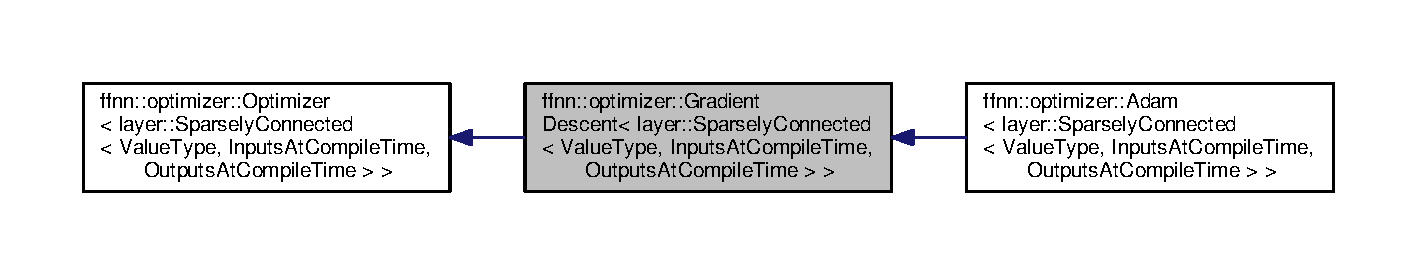
\includegraphics[width=350pt]{classffnn_1_1optimizer_1_1_gradient_descent_3_01layer_1_1_sparsely_connected_3_01_value_type_00_cd778e175158c5a4356ddedca0ec7368}
\end{center}
\end{figure}


Collaboration diagram for ffnn\-:\-:optimizer\-:\-:Gradient\-Descent$<$ layer\-:\-:Sparsely\-Connected$<$ Value\-Type, Inputs\-At\-Compile\-Time, Outputs\-At\-Compile\-Time $>$ $>$\-:\nopagebreak
\begin{figure}[H]
\begin{center}
\leavevmode
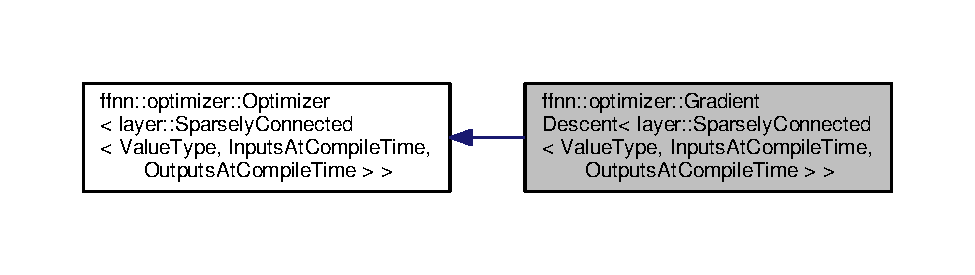
\includegraphics[width=350pt]{classffnn_1_1optimizer_1_1_gradient_descent_3_01layer_1_1_sparsely_connected_3_01_value_type_00_6ef3327b68786a574793ed94879a29cc}
\end{center}
\end{figure}
\subsection*{Public Types}
\begin{DoxyCompactItemize}
\item 
typedef \\*
layer\-::\-Sparsely\-Connected\\*
$<$ Value\-Type, \\*
Inputs\-At\-Compile\-Time, \\*
Outputs\-At\-Compile\-Time $>$ \hyperlink{classffnn_1_1optimizer_1_1_gradient_descent_3_01layer_1_1_sparsely_connected_3_01_value_type_00_e6c27913ab0d90f52f73031aa88c19bf_a87c420b734238a0c01d9928d224c649a}{Layer\-Type}
\begin{DoxyCompactList}\small\item\em Layer type standardization. \end{DoxyCompactList}\item 
typedef Layer\-Type\-::\-Scalar \hyperlink{classffnn_1_1optimizer_1_1_gradient_descent_3_01layer_1_1_sparsely_connected_3_01_value_type_00_e6c27913ab0d90f52f73031aa88c19bf_a5ee984a0be749179efea56cb46fe0eb1}{Scalar}
\begin{DoxyCompactList}\small\item\em Scalar type standardization. \end{DoxyCompactList}\item 
typedef Layer\-Type\-::\-Size\-Type \hyperlink{classffnn_1_1optimizer_1_1_gradient_descent_3_01layer_1_1_sparsely_connected_3_01_value_type_00_e6c27913ab0d90f52f73031aa88c19bf_a98715d1de7ba21998f64ec8e80051858}{Size\-Type}
\begin{DoxyCompactList}\small\item\em Size type standardization. \end{DoxyCompactList}\item 
typedef Layer\-Type\-::\-Input\-Block\-Type \hyperlink{classffnn_1_1optimizer_1_1_gradient_descent_3_01layer_1_1_sparsely_connected_3_01_value_type_00_e6c27913ab0d90f52f73031aa88c19bf_a06fa3b5a9d654609c0d90dcc09382e38}{Input\-Block\-Type}
\begin{DoxyCompactList}\small\item\em Matrix type standardization. \end{DoxyCompactList}\item 
typedef Layer\-Type\-::\-Output\-Block\-Type \hyperlink{classffnn_1_1optimizer_1_1_gradient_descent_3_01layer_1_1_sparsely_connected_3_01_value_type_00_e6c27913ab0d90f52f73031aa88c19bf_a3398102cd38960d104d31c868ecd9c06}{Output\-Block\-Type}
\begin{DoxyCompactList}\small\item\em Matrix type standardization. \end{DoxyCompactList}\item 
typedef Layer\-Type\-::\-Bias\-Vector\-Type \hyperlink{classffnn_1_1optimizer_1_1_gradient_descent_3_01layer_1_1_sparsely_connected_3_01_value_type_00_e6c27913ab0d90f52f73031aa88c19bf_a83473b9494908577009ea7edf1de1dfd}{Bias\-Vector\-Type}
\begin{DoxyCompactList}\small\item\em Bia vector type standardization. \end{DoxyCompactList}\item 
typedef Layer\-Type\-::\-Weight\-Matrix\-Type \hyperlink{classffnn_1_1optimizer_1_1_gradient_descent_3_01layer_1_1_sparsely_connected_3_01_value_type_00_e6c27913ab0d90f52f73031aa88c19bf_aac103d3f1c0095e1a195238254271ce1}{Weight\-Matrix\-Type}
\begin{DoxyCompactList}\small\item\em Input-\/output weight matrix. \end{DoxyCompactList}\end{DoxyCompactItemize}
\subsection*{Public Member Functions}
\begin{DoxyCompactItemize}
\item 
\hyperlink{classffnn_1_1optimizer_1_1_gradient_descent_3_01layer_1_1_sparsely_connected_3_01_value_type_00_e6c27913ab0d90f52f73031aa88c19bf_a330234323385bff90e9194498fd26ea0}{Gradient\-Descent} (\hyperlink{classffnn_1_1optimizer_1_1_gradient_descent_3_01layer_1_1_sparsely_connected_3_01_value_type_00_e6c27913ab0d90f52f73031aa88c19bf_a5ee984a0be749179efea56cb46fe0eb1}{Scalar} lr)
\begin{DoxyCompactList}\small\item\em Setup constructor. \end{DoxyCompactList}\item 
virtual \hyperlink{classffnn_1_1optimizer_1_1_gradient_descent_3_01layer_1_1_sparsely_connected_3_01_value_type_00_e6c27913ab0d90f52f73031aa88c19bf_a2df4cb253c287efa26fae8d7580d01e9}{$\sim$\-Gradient\-Descent} ()
\item 
virtual void \hyperlink{classffnn_1_1optimizer_1_1_gradient_descent_3_01layer_1_1_sparsely_connected_3_01_value_type_00_e6c27913ab0d90f52f73031aa88c19bf_ac3fa00e4febe86906ff6045fe77777b0}{initialize} (\hyperlink{classffnn_1_1optimizer_1_1_gradient_descent_3_01layer_1_1_sparsely_connected_3_01_value_type_00_e6c27913ab0d90f52f73031aa88c19bf_a87c420b734238a0c01d9928d224c649a}{Layer\-Type} \&layer)
\begin{DoxyCompactList}\small\item\em Initializes the \hyperlink{classffnn_1_1optimizer_1_1_optimizer}{Optimizer}. \end{DoxyCompactList}\item 
virtual void \hyperlink{classffnn_1_1optimizer_1_1_gradient_descent_3_01layer_1_1_sparsely_connected_3_01_value_type_00_e6c27913ab0d90f52f73031aa88c19bf_a61e4190921d10b1ec15f0a710b12df22}{reset} (\hyperlink{classffnn_1_1optimizer_1_1_gradient_descent_3_01layer_1_1_sparsely_connected_3_01_value_type_00_e6c27913ab0d90f52f73031aa88c19bf_a87c420b734238a0c01d9928d224c649a}{Layer\-Type} \&layer)
\begin{DoxyCompactList}\small\item\em Resetrs persistent \hyperlink{classffnn_1_1optimizer_1_1_optimizer}{Optimizer} states. \end{DoxyCompactList}\item 
virtual bool \hyperlink{classffnn_1_1optimizer_1_1_gradient_descent_3_01layer_1_1_sparsely_connected_3_01_value_type_00_e6c27913ab0d90f52f73031aa88c19bf_a7e9882cd69c5d4ee64f5614614e9d96c}{forward} (\hyperlink{classffnn_1_1optimizer_1_1_gradient_descent_3_01layer_1_1_sparsely_connected_3_01_value_type_00_e6c27913ab0d90f52f73031aa88c19bf_a87c420b734238a0c01d9928d224c649a}{Layer\-Type} \&layer)
\begin{DoxyCompactList}\small\item\em Computes one forward optimization update step. \end{DoxyCompactList}\item 
virtual bool \hyperlink{classffnn_1_1optimizer_1_1_gradient_descent_3_01layer_1_1_sparsely_connected_3_01_value_type_00_e6c27913ab0d90f52f73031aa88c19bf_a21e3b66b2d83b356b4534cf6d789fa18}{backward} (\hyperlink{classffnn_1_1optimizer_1_1_gradient_descent_3_01layer_1_1_sparsely_connected_3_01_value_type_00_e6c27913ab0d90f52f73031aa88c19bf_a87c420b734238a0c01d9928d224c649a}{Layer\-Type} \&layer)
\begin{DoxyCompactList}\small\item\em Computes optimization step during backward propogation. \end{DoxyCompactList}\item 
virtual bool \hyperlink{classffnn_1_1optimizer_1_1_gradient_descent_3_01layer_1_1_sparsely_connected_3_01_value_type_00_e6c27913ab0d90f52f73031aa88c19bf_ada280929e93a2d12f0bc21e9077e75a1}{update} (\hyperlink{classffnn_1_1optimizer_1_1_gradient_descent_3_01layer_1_1_sparsely_connected_3_01_value_type_00_e6c27913ab0d90f52f73031aa88c19bf_a87c420b734238a0c01d9928d224c649a}{Layer\-Type} \&layer)
\begin{DoxyCompactList}\small\item\em Applies optimization update. \end{DoxyCompactList}\end{DoxyCompactItemize}
\subsection*{Protected Attributes}
\begin{DoxyCompactItemize}
\item 
\hyperlink{classffnn_1_1optimizer_1_1_gradient_descent_3_01layer_1_1_sparsely_connected_3_01_value_type_00_e6c27913ab0d90f52f73031aa88c19bf_a5ee984a0be749179efea56cb46fe0eb1}{Scalar} \hyperlink{classffnn_1_1optimizer_1_1_gradient_descent_3_01layer_1_1_sparsely_connected_3_01_value_type_00_e6c27913ab0d90f52f73031aa88c19bf_a3bdbafb20c8bb1b0a7e1c9a745601537}{lr\-\_\-}
\begin{DoxyCompactList}\small\item\em Learning rate. \end{DoxyCompactList}\item 
\hyperlink{classffnn_1_1optimizer_1_1_gradient_descent_3_01layer_1_1_sparsely_connected_3_01_value_type_00_e6c27913ab0d90f52f73031aa88c19bf_aac103d3f1c0095e1a195238254271ce1}{Weight\-Matrix\-Type} \hyperlink{classffnn_1_1optimizer_1_1_gradient_descent_3_01layer_1_1_sparsely_connected_3_01_value_type_00_e6c27913ab0d90f52f73031aa88c19bf_a105f65dc92c783222f228fed80c52fda}{weight\-\_\-gradient\-\_\-}
\begin{DoxyCompactList}\small\item\em Weight matrix delta. \end{DoxyCompactList}\item 
\hyperlink{classffnn_1_1optimizer_1_1_gradient_descent_3_01layer_1_1_sparsely_connected_3_01_value_type_00_e6c27913ab0d90f52f73031aa88c19bf_a83473b9494908577009ea7edf1de1dfd}{Bias\-Vector\-Type} \hyperlink{classffnn_1_1optimizer_1_1_gradient_descent_3_01layer_1_1_sparsely_connected_3_01_value_type_00_e6c27913ab0d90f52f73031aa88c19bf_a38013045946f2a6d8a30445c9048654f}{bias\-\_\-gradient\-\_\-}
\begin{DoxyCompactList}\small\item\em Total bias vector delta. \end{DoxyCompactList}\item 
\hyperlink{classffnn_1_1optimizer_1_1_gradient_descent_3_01layer_1_1_sparsely_connected_3_01_value_type_00_e6c27913ab0d90f52f73031aa88c19bf_a06fa3b5a9d654609c0d90dcc09382e38}{Input\-Block\-Type} \hyperlink{classffnn_1_1optimizer_1_1_gradient_descent_3_01layer_1_1_sparsely_connected_3_01_value_type_00_e6c27913ab0d90f52f73031aa88c19bf_acce1f255ec414b8eddef1429398bccce}{prev\-\_\-input\-\_\-}
\begin{DoxyCompactList}\small\item\em Previous input. \end{DoxyCompactList}\end{DoxyCompactItemize}


\subsection{Member Typedef Documentation}
\hypertarget{classffnn_1_1optimizer_1_1_gradient_descent_3_01layer_1_1_sparsely_connected_3_01_value_type_00_e6c27913ab0d90f52f73031aa88c19bf_a83473b9494908577009ea7edf1de1dfd}{\index{ffnn\-::optimizer\-::\-Gradient\-Descent$<$ layer\-::\-Sparsely\-Connected$<$ Value\-Type, Inputs\-At\-Compile\-Time, Outputs\-At\-Compile\-Time $>$ $>$@{ffnn\-::optimizer\-::\-Gradient\-Descent$<$ layer\-::\-Sparsely\-Connected$<$ Value\-Type, Inputs\-At\-Compile\-Time, Outputs\-At\-Compile\-Time $>$ $>$}!Bias\-Vector\-Type@{Bias\-Vector\-Type}}
\index{Bias\-Vector\-Type@{Bias\-Vector\-Type}!ffnn::optimizer::GradientDescent< layer::SparselyConnected< ValueType, InputsAtCompileTime, OutputsAtCompileTime > >@{ffnn\-::optimizer\-::\-Gradient\-Descent$<$ layer\-::\-Sparsely\-Connected$<$ Value\-Type, Inputs\-At\-Compile\-Time, Outputs\-At\-Compile\-Time $>$ $>$}}
\subsubsection[{Bias\-Vector\-Type}]{\setlength{\rightskip}{0pt plus 5cm}typedef Layer\-Type\-::\-Bias\-Vector\-Type {\bf ffnn\-::optimizer\-::\-Gradient\-Descent}$<$ layer\-::\-Sparsely\-Connected$<$ Value\-Type, Inputs\-At\-Compile\-Time, Outputs\-At\-Compile\-Time $>$ $>$\-::{\bf Bias\-Vector\-Type}}}\label{classffnn_1_1optimizer_1_1_gradient_descent_3_01layer_1_1_sparsely_connected_3_01_value_type_00_e6c27913ab0d90f52f73031aa88c19bf_a83473b9494908577009ea7edf1de1dfd}


Bia vector type standardization. 

\hypertarget{classffnn_1_1optimizer_1_1_gradient_descent_3_01layer_1_1_sparsely_connected_3_01_value_type_00_e6c27913ab0d90f52f73031aa88c19bf_a06fa3b5a9d654609c0d90dcc09382e38}{\index{ffnn\-::optimizer\-::\-Gradient\-Descent$<$ layer\-::\-Sparsely\-Connected$<$ Value\-Type, Inputs\-At\-Compile\-Time, Outputs\-At\-Compile\-Time $>$ $>$@{ffnn\-::optimizer\-::\-Gradient\-Descent$<$ layer\-::\-Sparsely\-Connected$<$ Value\-Type, Inputs\-At\-Compile\-Time, Outputs\-At\-Compile\-Time $>$ $>$}!Input\-Block\-Type@{Input\-Block\-Type}}
\index{Input\-Block\-Type@{Input\-Block\-Type}!ffnn::optimizer::GradientDescent< layer::SparselyConnected< ValueType, InputsAtCompileTime, OutputsAtCompileTime > >@{ffnn\-::optimizer\-::\-Gradient\-Descent$<$ layer\-::\-Sparsely\-Connected$<$ Value\-Type, Inputs\-At\-Compile\-Time, Outputs\-At\-Compile\-Time $>$ $>$}}
\subsubsection[{Input\-Block\-Type}]{\setlength{\rightskip}{0pt plus 5cm}typedef Layer\-Type\-::\-Input\-Block\-Type {\bf ffnn\-::optimizer\-::\-Gradient\-Descent}$<$ layer\-::\-Sparsely\-Connected$<$ Value\-Type, Inputs\-At\-Compile\-Time, Outputs\-At\-Compile\-Time $>$ $>$\-::{\bf Input\-Block\-Type}}}\label{classffnn_1_1optimizer_1_1_gradient_descent_3_01layer_1_1_sparsely_connected_3_01_value_type_00_e6c27913ab0d90f52f73031aa88c19bf_a06fa3b5a9d654609c0d90dcc09382e38}


Matrix type standardization. 

\hypertarget{classffnn_1_1optimizer_1_1_gradient_descent_3_01layer_1_1_sparsely_connected_3_01_value_type_00_e6c27913ab0d90f52f73031aa88c19bf_a87c420b734238a0c01d9928d224c649a}{\index{ffnn\-::optimizer\-::\-Gradient\-Descent$<$ layer\-::\-Sparsely\-Connected$<$ Value\-Type, Inputs\-At\-Compile\-Time, Outputs\-At\-Compile\-Time $>$ $>$@{ffnn\-::optimizer\-::\-Gradient\-Descent$<$ layer\-::\-Sparsely\-Connected$<$ Value\-Type, Inputs\-At\-Compile\-Time, Outputs\-At\-Compile\-Time $>$ $>$}!Layer\-Type@{Layer\-Type}}
\index{Layer\-Type@{Layer\-Type}!ffnn::optimizer::GradientDescent< layer::SparselyConnected< ValueType, InputsAtCompileTime, OutputsAtCompileTime > >@{ffnn\-::optimizer\-::\-Gradient\-Descent$<$ layer\-::\-Sparsely\-Connected$<$ Value\-Type, Inputs\-At\-Compile\-Time, Outputs\-At\-Compile\-Time $>$ $>$}}
\subsubsection[{Layer\-Type}]{\setlength{\rightskip}{0pt plus 5cm}typedef layer\-::\-Sparsely\-Connected$<$Value\-Type, Inputs\-At\-Compile\-Time, Outputs\-At\-Compile\-Time$>$ {\bf ffnn\-::optimizer\-::\-Gradient\-Descent}$<$ layer\-::\-Sparsely\-Connected$<$ Value\-Type, Inputs\-At\-Compile\-Time, Outputs\-At\-Compile\-Time $>$ $>$\-::{\bf Layer\-Type}}}\label{classffnn_1_1optimizer_1_1_gradient_descent_3_01layer_1_1_sparsely_connected_3_01_value_type_00_e6c27913ab0d90f52f73031aa88c19bf_a87c420b734238a0c01d9928d224c649a}


Layer type standardization. 

\hypertarget{classffnn_1_1optimizer_1_1_gradient_descent_3_01layer_1_1_sparsely_connected_3_01_value_type_00_e6c27913ab0d90f52f73031aa88c19bf_a3398102cd38960d104d31c868ecd9c06}{\index{ffnn\-::optimizer\-::\-Gradient\-Descent$<$ layer\-::\-Sparsely\-Connected$<$ Value\-Type, Inputs\-At\-Compile\-Time, Outputs\-At\-Compile\-Time $>$ $>$@{ffnn\-::optimizer\-::\-Gradient\-Descent$<$ layer\-::\-Sparsely\-Connected$<$ Value\-Type, Inputs\-At\-Compile\-Time, Outputs\-At\-Compile\-Time $>$ $>$}!Output\-Block\-Type@{Output\-Block\-Type}}
\index{Output\-Block\-Type@{Output\-Block\-Type}!ffnn::optimizer::GradientDescent< layer::SparselyConnected< ValueType, InputsAtCompileTime, OutputsAtCompileTime > >@{ffnn\-::optimizer\-::\-Gradient\-Descent$<$ layer\-::\-Sparsely\-Connected$<$ Value\-Type, Inputs\-At\-Compile\-Time, Outputs\-At\-Compile\-Time $>$ $>$}}
\subsubsection[{Output\-Block\-Type}]{\setlength{\rightskip}{0pt plus 5cm}typedef Layer\-Type\-::\-Output\-Block\-Type {\bf ffnn\-::optimizer\-::\-Gradient\-Descent}$<$ layer\-::\-Sparsely\-Connected$<$ Value\-Type, Inputs\-At\-Compile\-Time, Outputs\-At\-Compile\-Time $>$ $>$\-::{\bf Output\-Block\-Type}}}\label{classffnn_1_1optimizer_1_1_gradient_descent_3_01layer_1_1_sparsely_connected_3_01_value_type_00_e6c27913ab0d90f52f73031aa88c19bf_a3398102cd38960d104d31c868ecd9c06}


Matrix type standardization. 

\hypertarget{classffnn_1_1optimizer_1_1_gradient_descent_3_01layer_1_1_sparsely_connected_3_01_value_type_00_e6c27913ab0d90f52f73031aa88c19bf_a5ee984a0be749179efea56cb46fe0eb1}{\index{ffnn\-::optimizer\-::\-Gradient\-Descent$<$ layer\-::\-Sparsely\-Connected$<$ Value\-Type, Inputs\-At\-Compile\-Time, Outputs\-At\-Compile\-Time $>$ $>$@{ffnn\-::optimizer\-::\-Gradient\-Descent$<$ layer\-::\-Sparsely\-Connected$<$ Value\-Type, Inputs\-At\-Compile\-Time, Outputs\-At\-Compile\-Time $>$ $>$}!Scalar@{Scalar}}
\index{Scalar@{Scalar}!ffnn::optimizer::GradientDescent< layer::SparselyConnected< ValueType, InputsAtCompileTime, OutputsAtCompileTime > >@{ffnn\-::optimizer\-::\-Gradient\-Descent$<$ layer\-::\-Sparsely\-Connected$<$ Value\-Type, Inputs\-At\-Compile\-Time, Outputs\-At\-Compile\-Time $>$ $>$}}
\subsubsection[{Scalar}]{\setlength{\rightskip}{0pt plus 5cm}typedef Layer\-Type\-::\-Scalar {\bf ffnn\-::optimizer\-::\-Gradient\-Descent}$<$ layer\-::\-Sparsely\-Connected$<$ Value\-Type, Inputs\-At\-Compile\-Time, Outputs\-At\-Compile\-Time $>$ $>$\-::{\bf Scalar}}}\label{classffnn_1_1optimizer_1_1_gradient_descent_3_01layer_1_1_sparsely_connected_3_01_value_type_00_e6c27913ab0d90f52f73031aa88c19bf_a5ee984a0be749179efea56cb46fe0eb1}


Scalar type standardization. 

\hypertarget{classffnn_1_1optimizer_1_1_gradient_descent_3_01layer_1_1_sparsely_connected_3_01_value_type_00_e6c27913ab0d90f52f73031aa88c19bf_a98715d1de7ba21998f64ec8e80051858}{\index{ffnn\-::optimizer\-::\-Gradient\-Descent$<$ layer\-::\-Sparsely\-Connected$<$ Value\-Type, Inputs\-At\-Compile\-Time, Outputs\-At\-Compile\-Time $>$ $>$@{ffnn\-::optimizer\-::\-Gradient\-Descent$<$ layer\-::\-Sparsely\-Connected$<$ Value\-Type, Inputs\-At\-Compile\-Time, Outputs\-At\-Compile\-Time $>$ $>$}!Size\-Type@{Size\-Type}}
\index{Size\-Type@{Size\-Type}!ffnn::optimizer::GradientDescent< layer::SparselyConnected< ValueType, InputsAtCompileTime, OutputsAtCompileTime > >@{ffnn\-::optimizer\-::\-Gradient\-Descent$<$ layer\-::\-Sparsely\-Connected$<$ Value\-Type, Inputs\-At\-Compile\-Time, Outputs\-At\-Compile\-Time $>$ $>$}}
\subsubsection[{Size\-Type}]{\setlength{\rightskip}{0pt plus 5cm}typedef Layer\-Type\-::\-Size\-Type {\bf ffnn\-::optimizer\-::\-Gradient\-Descent}$<$ layer\-::\-Sparsely\-Connected$<$ Value\-Type, Inputs\-At\-Compile\-Time, Outputs\-At\-Compile\-Time $>$ $>$\-::{\bf Size\-Type}}}\label{classffnn_1_1optimizer_1_1_gradient_descent_3_01layer_1_1_sparsely_connected_3_01_value_type_00_e6c27913ab0d90f52f73031aa88c19bf_a98715d1de7ba21998f64ec8e80051858}


Size type standardization. 

\hypertarget{classffnn_1_1optimizer_1_1_gradient_descent_3_01layer_1_1_sparsely_connected_3_01_value_type_00_e6c27913ab0d90f52f73031aa88c19bf_aac103d3f1c0095e1a195238254271ce1}{\index{ffnn\-::optimizer\-::\-Gradient\-Descent$<$ layer\-::\-Sparsely\-Connected$<$ Value\-Type, Inputs\-At\-Compile\-Time, Outputs\-At\-Compile\-Time $>$ $>$@{ffnn\-::optimizer\-::\-Gradient\-Descent$<$ layer\-::\-Sparsely\-Connected$<$ Value\-Type, Inputs\-At\-Compile\-Time, Outputs\-At\-Compile\-Time $>$ $>$}!Weight\-Matrix\-Type@{Weight\-Matrix\-Type}}
\index{Weight\-Matrix\-Type@{Weight\-Matrix\-Type}!ffnn::optimizer::GradientDescent< layer::SparselyConnected< ValueType, InputsAtCompileTime, OutputsAtCompileTime > >@{ffnn\-::optimizer\-::\-Gradient\-Descent$<$ layer\-::\-Sparsely\-Connected$<$ Value\-Type, Inputs\-At\-Compile\-Time, Outputs\-At\-Compile\-Time $>$ $>$}}
\subsubsection[{Weight\-Matrix\-Type}]{\setlength{\rightskip}{0pt plus 5cm}typedef Layer\-Type\-::\-Weight\-Matrix\-Type {\bf ffnn\-::optimizer\-::\-Gradient\-Descent}$<$ layer\-::\-Sparsely\-Connected$<$ Value\-Type, Inputs\-At\-Compile\-Time, Outputs\-At\-Compile\-Time $>$ $>$\-::{\bf Weight\-Matrix\-Type}}}\label{classffnn_1_1optimizer_1_1_gradient_descent_3_01layer_1_1_sparsely_connected_3_01_value_type_00_e6c27913ab0d90f52f73031aa88c19bf_aac103d3f1c0095e1a195238254271ce1}


Input-\/output weight matrix. 



\subsection{Constructor \& Destructor Documentation}
\hypertarget{classffnn_1_1optimizer_1_1_gradient_descent_3_01layer_1_1_sparsely_connected_3_01_value_type_00_e6c27913ab0d90f52f73031aa88c19bf_a330234323385bff90e9194498fd26ea0}{\index{ffnn\-::optimizer\-::\-Gradient\-Descent$<$ layer\-::\-Sparsely\-Connected$<$ Value\-Type, Inputs\-At\-Compile\-Time, Outputs\-At\-Compile\-Time $>$ $>$@{ffnn\-::optimizer\-::\-Gradient\-Descent$<$ layer\-::\-Sparsely\-Connected$<$ Value\-Type, Inputs\-At\-Compile\-Time, Outputs\-At\-Compile\-Time $>$ $>$}!Gradient\-Descent@{Gradient\-Descent}}
\index{Gradient\-Descent@{Gradient\-Descent}!ffnn::optimizer::GradientDescent< layer::SparselyConnected< ValueType, InputsAtCompileTime, OutputsAtCompileTime > >@{ffnn\-::optimizer\-::\-Gradient\-Descent$<$ layer\-::\-Sparsely\-Connected$<$ Value\-Type, Inputs\-At\-Compile\-Time, Outputs\-At\-Compile\-Time $>$ $>$}}
\subsubsection[{Gradient\-Descent}]{\setlength{\rightskip}{0pt plus 5cm}{\bf ffnn\-::optimizer\-::\-Gradient\-Descent}$<$ layer\-::\-Sparsely\-Connected$<$ Value\-Type, Inputs\-At\-Compile\-Time, Outputs\-At\-Compile\-Time $>$ $>$\-::{\bf Gradient\-Descent} (
\begin{DoxyParamCaption}
\item[{{\bf Scalar}}]{lr}
\end{DoxyParamCaption}
)\hspace{0.3cm}{\ttfamily [inline]}, {\ttfamily [explicit]}}}\label{classffnn_1_1optimizer_1_1_gradient_descent_3_01layer_1_1_sparsely_connected_3_01_value_type_00_e6c27913ab0d90f52f73031aa88c19bf_a330234323385bff90e9194498fd26ea0}


Setup constructor. 


\begin{DoxyParams}{Parameters}
{\em lr} & Learning rate \\
\hline
\end{DoxyParams}
\hypertarget{classffnn_1_1optimizer_1_1_gradient_descent_3_01layer_1_1_sparsely_connected_3_01_value_type_00_e6c27913ab0d90f52f73031aa88c19bf_a2df4cb253c287efa26fae8d7580d01e9}{\index{ffnn\-::optimizer\-::\-Gradient\-Descent$<$ layer\-::\-Sparsely\-Connected$<$ Value\-Type, Inputs\-At\-Compile\-Time, Outputs\-At\-Compile\-Time $>$ $>$@{ffnn\-::optimizer\-::\-Gradient\-Descent$<$ layer\-::\-Sparsely\-Connected$<$ Value\-Type, Inputs\-At\-Compile\-Time, Outputs\-At\-Compile\-Time $>$ $>$}!$\sim$\-Gradient\-Descent@{$\sim$\-Gradient\-Descent}}
\index{$\sim$\-Gradient\-Descent@{$\sim$\-Gradient\-Descent}!ffnn::optimizer::GradientDescent< layer::SparselyConnected< ValueType, InputsAtCompileTime, OutputsAtCompileTime > >@{ffnn\-::optimizer\-::\-Gradient\-Descent$<$ layer\-::\-Sparsely\-Connected$<$ Value\-Type, Inputs\-At\-Compile\-Time, Outputs\-At\-Compile\-Time $>$ $>$}}
\subsubsection[{$\sim$\-Gradient\-Descent}]{\setlength{\rightskip}{0pt plus 5cm}virtual {\bf ffnn\-::optimizer\-::\-Gradient\-Descent}$<$ layer\-::\-Sparsely\-Connected$<$ Value\-Type, Inputs\-At\-Compile\-Time, Outputs\-At\-Compile\-Time $>$ $>$\-::$\sim${\bf Gradient\-Descent} (
\begin{DoxyParamCaption}
{}
\end{DoxyParamCaption}
)\hspace{0.3cm}{\ttfamily [inline]}, {\ttfamily [virtual]}}}\label{classffnn_1_1optimizer_1_1_gradient_descent_3_01layer_1_1_sparsely_connected_3_01_value_type_00_e6c27913ab0d90f52f73031aa88c19bf_a2df4cb253c287efa26fae8d7580d01e9}


\subsection{Member Function Documentation}
\hypertarget{classffnn_1_1optimizer_1_1_gradient_descent_3_01layer_1_1_sparsely_connected_3_01_value_type_00_e6c27913ab0d90f52f73031aa88c19bf_a21e3b66b2d83b356b4534cf6d789fa18}{\index{ffnn\-::optimizer\-::\-Gradient\-Descent$<$ layer\-::\-Sparsely\-Connected$<$ Value\-Type, Inputs\-At\-Compile\-Time, Outputs\-At\-Compile\-Time $>$ $>$@{ffnn\-::optimizer\-::\-Gradient\-Descent$<$ layer\-::\-Sparsely\-Connected$<$ Value\-Type, Inputs\-At\-Compile\-Time, Outputs\-At\-Compile\-Time $>$ $>$}!backward@{backward}}
\index{backward@{backward}!ffnn::optimizer::GradientDescent< layer::SparselyConnected< ValueType, InputsAtCompileTime, OutputsAtCompileTime > >@{ffnn\-::optimizer\-::\-Gradient\-Descent$<$ layer\-::\-Sparsely\-Connected$<$ Value\-Type, Inputs\-At\-Compile\-Time, Outputs\-At\-Compile\-Time $>$ $>$}}
\subsubsection[{backward}]{\setlength{\rightskip}{0pt plus 5cm}virtual bool {\bf ffnn\-::optimizer\-::\-Gradient\-Descent}$<$ layer\-::\-Sparsely\-Connected$<$ Value\-Type, Inputs\-At\-Compile\-Time, Outputs\-At\-Compile\-Time $>$ $>$\-::backward (
\begin{DoxyParamCaption}
\item[{{\bf Layer\-Type} \&}]{layer}
\end{DoxyParamCaption}
)\hspace{0.3cm}{\ttfamily [inline]}, {\ttfamily [virtual]}}}\label{classffnn_1_1optimizer_1_1_gradient_descent_3_01layer_1_1_sparsely_connected_3_01_value_type_00_e6c27913ab0d90f52f73031aa88c19bf_a21e3b66b2d83b356b4534cf6d789fa18}


Computes optimization step during backward propogation. 


\begin{DoxyParams}[1]{Parameters}
\mbox{\tt in,out}  & {\em layer} & Layer to optimize \\
\hline
\end{DoxyParams}

\begin{DoxyRetVals}{Return values}
{\em true} & if optimization setp was successful \\
\hline
{\em false} & otherwise \\
\hline
\end{DoxyRetVals}


Implements \hyperlink{classffnn_1_1optimizer_1_1_optimizer_ab1f9b1cae01f93f53ecf7119bedb6369}{ffnn\-::optimizer\-::\-Optimizer$<$ layer\-::\-Sparsely\-Connected$<$ Value\-Type, Inputs\-At\-Compile\-Time, Outputs\-At\-Compile\-Time $>$ $>$}.

\hypertarget{classffnn_1_1optimizer_1_1_gradient_descent_3_01layer_1_1_sparsely_connected_3_01_value_type_00_e6c27913ab0d90f52f73031aa88c19bf_a7e9882cd69c5d4ee64f5614614e9d96c}{\index{ffnn\-::optimizer\-::\-Gradient\-Descent$<$ layer\-::\-Sparsely\-Connected$<$ Value\-Type, Inputs\-At\-Compile\-Time, Outputs\-At\-Compile\-Time $>$ $>$@{ffnn\-::optimizer\-::\-Gradient\-Descent$<$ layer\-::\-Sparsely\-Connected$<$ Value\-Type, Inputs\-At\-Compile\-Time, Outputs\-At\-Compile\-Time $>$ $>$}!forward@{forward}}
\index{forward@{forward}!ffnn::optimizer::GradientDescent< layer::SparselyConnected< ValueType, InputsAtCompileTime, OutputsAtCompileTime > >@{ffnn\-::optimizer\-::\-Gradient\-Descent$<$ layer\-::\-Sparsely\-Connected$<$ Value\-Type, Inputs\-At\-Compile\-Time, Outputs\-At\-Compile\-Time $>$ $>$}}
\subsubsection[{forward}]{\setlength{\rightskip}{0pt plus 5cm}virtual bool {\bf ffnn\-::optimizer\-::\-Gradient\-Descent}$<$ layer\-::\-Sparsely\-Connected$<$ Value\-Type, Inputs\-At\-Compile\-Time, Outputs\-At\-Compile\-Time $>$ $>$\-::forward (
\begin{DoxyParamCaption}
\item[{{\bf Layer\-Type} \&}]{layer}
\end{DoxyParamCaption}
)\hspace{0.3cm}{\ttfamily [inline]}, {\ttfamily [virtual]}}}\label{classffnn_1_1optimizer_1_1_gradient_descent_3_01layer_1_1_sparsely_connected_3_01_value_type_00_e6c27913ab0d90f52f73031aa88c19bf_a7e9882cd69c5d4ee64f5614614e9d96c}


Computes one forward optimization update step. 


\begin{DoxyParams}[1]{Parameters}
\mbox{\tt in,out}  & {\em layer} & Layer to optimize \\
\hline
\end{DoxyParams}

\begin{DoxyRetVals}{Return values}
{\em true} & if optimization setp was successful \\
\hline
{\em false} & otherwise \\
\hline
\end{DoxyRetVals}


Implements \hyperlink{classffnn_1_1optimizer_1_1_optimizer_a80505cfdeba0a3c8d1db19a2821613f2}{ffnn\-::optimizer\-::\-Optimizer$<$ layer\-::\-Sparsely\-Connected$<$ Value\-Type, Inputs\-At\-Compile\-Time, Outputs\-At\-Compile\-Time $>$ $>$}.

\hypertarget{classffnn_1_1optimizer_1_1_gradient_descent_3_01layer_1_1_sparsely_connected_3_01_value_type_00_e6c27913ab0d90f52f73031aa88c19bf_ac3fa00e4febe86906ff6045fe77777b0}{\index{ffnn\-::optimizer\-::\-Gradient\-Descent$<$ layer\-::\-Sparsely\-Connected$<$ Value\-Type, Inputs\-At\-Compile\-Time, Outputs\-At\-Compile\-Time $>$ $>$@{ffnn\-::optimizer\-::\-Gradient\-Descent$<$ layer\-::\-Sparsely\-Connected$<$ Value\-Type, Inputs\-At\-Compile\-Time, Outputs\-At\-Compile\-Time $>$ $>$}!initialize@{initialize}}
\index{initialize@{initialize}!ffnn::optimizer::GradientDescent< layer::SparselyConnected< ValueType, InputsAtCompileTime, OutputsAtCompileTime > >@{ffnn\-::optimizer\-::\-Gradient\-Descent$<$ layer\-::\-Sparsely\-Connected$<$ Value\-Type, Inputs\-At\-Compile\-Time, Outputs\-At\-Compile\-Time $>$ $>$}}
\subsubsection[{initialize}]{\setlength{\rightskip}{0pt plus 5cm}virtual void {\bf ffnn\-::optimizer\-::\-Gradient\-Descent}$<$ layer\-::\-Sparsely\-Connected$<$ Value\-Type, Inputs\-At\-Compile\-Time, Outputs\-At\-Compile\-Time $>$ $>$\-::initialize (
\begin{DoxyParamCaption}
\item[{{\bf Layer\-Type} \&}]{layer}
\end{DoxyParamCaption}
)\hspace{0.3cm}{\ttfamily [inline]}, {\ttfamily [virtual]}}}\label{classffnn_1_1optimizer_1_1_gradient_descent_3_01layer_1_1_sparsely_connected_3_01_value_type_00_e6c27913ab0d90f52f73031aa88c19bf_ac3fa00e4febe86906ff6045fe77777b0}


Initializes the \hyperlink{classffnn_1_1optimizer_1_1_optimizer}{Optimizer}. 


\begin{DoxyParams}[1]{Parameters}
\mbox{\tt in,out}  & {\em layer} & Layer to optimize \\
\hline
\end{DoxyParams}


Implements \hyperlink{classffnn_1_1optimizer_1_1_optimizer_a4302b66ba9b013ae4833eca235ff306a}{ffnn\-::optimizer\-::\-Optimizer$<$ layer\-::\-Sparsely\-Connected$<$ Value\-Type, Inputs\-At\-Compile\-Time, Outputs\-At\-Compile\-Time $>$ $>$}.



Reimplemented in \hyperlink{classffnn_1_1optimizer_1_1_adam_3_01layer_1_1_sparsely_connected_3_01_value_type_00_01_inputs_at5101e46d32858ec2169acdeede08d723_a3529c6f6fb1befc882cc3ae17c00ba5a}{ffnn\-::optimizer\-::\-Adam$<$ layer\-::\-Sparsely\-Connected$<$ Value\-Type, Inputs\-At\-Compile\-Time, Outputs\-At\-Compile\-Time $>$ $>$}.

\hypertarget{classffnn_1_1optimizer_1_1_gradient_descent_3_01layer_1_1_sparsely_connected_3_01_value_type_00_e6c27913ab0d90f52f73031aa88c19bf_a61e4190921d10b1ec15f0a710b12df22}{\index{ffnn\-::optimizer\-::\-Gradient\-Descent$<$ layer\-::\-Sparsely\-Connected$<$ Value\-Type, Inputs\-At\-Compile\-Time, Outputs\-At\-Compile\-Time $>$ $>$@{ffnn\-::optimizer\-::\-Gradient\-Descent$<$ layer\-::\-Sparsely\-Connected$<$ Value\-Type, Inputs\-At\-Compile\-Time, Outputs\-At\-Compile\-Time $>$ $>$}!reset@{reset}}
\index{reset@{reset}!ffnn::optimizer::GradientDescent< layer::SparselyConnected< ValueType, InputsAtCompileTime, OutputsAtCompileTime > >@{ffnn\-::optimizer\-::\-Gradient\-Descent$<$ layer\-::\-Sparsely\-Connected$<$ Value\-Type, Inputs\-At\-Compile\-Time, Outputs\-At\-Compile\-Time $>$ $>$}}
\subsubsection[{reset}]{\setlength{\rightskip}{0pt plus 5cm}virtual void {\bf ffnn\-::optimizer\-::\-Gradient\-Descent}$<$ layer\-::\-Sparsely\-Connected$<$ Value\-Type, Inputs\-At\-Compile\-Time, Outputs\-At\-Compile\-Time $>$ $>$\-::reset (
\begin{DoxyParamCaption}
\item[{{\bf Layer\-Type} \&}]{layer}
\end{DoxyParamCaption}
)\hspace{0.3cm}{\ttfamily [inline]}, {\ttfamily [virtual]}}}\label{classffnn_1_1optimizer_1_1_gradient_descent_3_01layer_1_1_sparsely_connected_3_01_value_type_00_e6c27913ab0d90f52f73031aa88c19bf_a61e4190921d10b1ec15f0a710b12df22}


Resetrs persistent \hyperlink{classffnn_1_1optimizer_1_1_optimizer}{Optimizer} states. 


\begin{DoxyParams}[1]{Parameters}
\mbox{\tt in,out}  & {\em layer} & Layer to optimize \\
\hline
\end{DoxyParams}


Implements \hyperlink{classffnn_1_1optimizer_1_1_optimizer_ade04e7582eb7b833713a9bd33e0e8346}{ffnn\-::optimizer\-::\-Optimizer$<$ layer\-::\-Sparsely\-Connected$<$ Value\-Type, Inputs\-At\-Compile\-Time, Outputs\-At\-Compile\-Time $>$ $>$}.

\hypertarget{classffnn_1_1optimizer_1_1_gradient_descent_3_01layer_1_1_sparsely_connected_3_01_value_type_00_e6c27913ab0d90f52f73031aa88c19bf_ada280929e93a2d12f0bc21e9077e75a1}{\index{ffnn\-::optimizer\-::\-Gradient\-Descent$<$ layer\-::\-Sparsely\-Connected$<$ Value\-Type, Inputs\-At\-Compile\-Time, Outputs\-At\-Compile\-Time $>$ $>$@{ffnn\-::optimizer\-::\-Gradient\-Descent$<$ layer\-::\-Sparsely\-Connected$<$ Value\-Type, Inputs\-At\-Compile\-Time, Outputs\-At\-Compile\-Time $>$ $>$}!update@{update}}
\index{update@{update}!ffnn::optimizer::GradientDescent< layer::SparselyConnected< ValueType, InputsAtCompileTime, OutputsAtCompileTime > >@{ffnn\-::optimizer\-::\-Gradient\-Descent$<$ layer\-::\-Sparsely\-Connected$<$ Value\-Type, Inputs\-At\-Compile\-Time, Outputs\-At\-Compile\-Time $>$ $>$}}
\subsubsection[{update}]{\setlength{\rightskip}{0pt plus 5cm}virtual bool {\bf ffnn\-::optimizer\-::\-Gradient\-Descent}$<$ layer\-::\-Sparsely\-Connected$<$ Value\-Type, Inputs\-At\-Compile\-Time, Outputs\-At\-Compile\-Time $>$ $>$\-::update (
\begin{DoxyParamCaption}
\item[{{\bf Layer\-Type} \&}]{layer}
\end{DoxyParamCaption}
)\hspace{0.3cm}{\ttfamily [inline]}, {\ttfamily [virtual]}}}\label{classffnn_1_1optimizer_1_1_gradient_descent_3_01layer_1_1_sparsely_connected_3_01_value_type_00_e6c27913ab0d90f52f73031aa88c19bf_ada280929e93a2d12f0bc21e9077e75a1}


Applies optimization update. 


\begin{DoxyParams}[1]{Parameters}
\mbox{\tt in,out}  & {\em layer} & Layer to optimize \\
\hline
\end{DoxyParams}

\begin{DoxyRetVals}{Return values}
{\em true} & if optimization update was applied successfully \\
\hline
{\em false} & otherwise \\
\hline
\end{DoxyRetVals}


Implements \hyperlink{classffnn_1_1optimizer_1_1_optimizer_a7c88c2794446e03ccd41628bb25d7a07}{ffnn\-::optimizer\-::\-Optimizer$<$ layer\-::\-Sparsely\-Connected$<$ Value\-Type, Inputs\-At\-Compile\-Time, Outputs\-At\-Compile\-Time $>$ $>$}.



Reimplemented in \hyperlink{classffnn_1_1optimizer_1_1_adam_3_01layer_1_1_sparsely_connected_3_01_value_type_00_01_inputs_at5101e46d32858ec2169acdeede08d723_aaa3b2eb55a9d80d51330c132df65214b}{ffnn\-::optimizer\-::\-Adam$<$ layer\-::\-Sparsely\-Connected$<$ Value\-Type, Inputs\-At\-Compile\-Time, Outputs\-At\-Compile\-Time $>$ $>$}.



\subsection{Member Data Documentation}
\hypertarget{classffnn_1_1optimizer_1_1_gradient_descent_3_01layer_1_1_sparsely_connected_3_01_value_type_00_e6c27913ab0d90f52f73031aa88c19bf_a38013045946f2a6d8a30445c9048654f}{\index{ffnn\-::optimizer\-::\-Gradient\-Descent$<$ layer\-::\-Sparsely\-Connected$<$ Value\-Type, Inputs\-At\-Compile\-Time, Outputs\-At\-Compile\-Time $>$ $>$@{ffnn\-::optimizer\-::\-Gradient\-Descent$<$ layer\-::\-Sparsely\-Connected$<$ Value\-Type, Inputs\-At\-Compile\-Time, Outputs\-At\-Compile\-Time $>$ $>$}!bias\-\_\-gradient\-\_\-@{bias\-\_\-gradient\-\_\-}}
\index{bias\-\_\-gradient\-\_\-@{bias\-\_\-gradient\-\_\-}!ffnn::optimizer::GradientDescent< layer::SparselyConnected< ValueType, InputsAtCompileTime, OutputsAtCompileTime > >@{ffnn\-::optimizer\-::\-Gradient\-Descent$<$ layer\-::\-Sparsely\-Connected$<$ Value\-Type, Inputs\-At\-Compile\-Time, Outputs\-At\-Compile\-Time $>$ $>$}}
\subsubsection[{bias\-\_\-gradient\-\_\-}]{\setlength{\rightskip}{0pt plus 5cm}{\bf Bias\-Vector\-Type} {\bf ffnn\-::optimizer\-::\-Gradient\-Descent}$<$ layer\-::\-Sparsely\-Connected$<$ Value\-Type, Inputs\-At\-Compile\-Time, Outputs\-At\-Compile\-Time $>$ $>$\-::bias\-\_\-gradient\-\_\-\hspace{0.3cm}{\ttfamily [protected]}}}\label{classffnn_1_1optimizer_1_1_gradient_descent_3_01layer_1_1_sparsely_connected_3_01_value_type_00_e6c27913ab0d90f52f73031aa88c19bf_a38013045946f2a6d8a30445c9048654f}


Total bias vector delta. 

\hypertarget{classffnn_1_1optimizer_1_1_gradient_descent_3_01layer_1_1_sparsely_connected_3_01_value_type_00_e6c27913ab0d90f52f73031aa88c19bf_a3bdbafb20c8bb1b0a7e1c9a745601537}{\index{ffnn\-::optimizer\-::\-Gradient\-Descent$<$ layer\-::\-Sparsely\-Connected$<$ Value\-Type, Inputs\-At\-Compile\-Time, Outputs\-At\-Compile\-Time $>$ $>$@{ffnn\-::optimizer\-::\-Gradient\-Descent$<$ layer\-::\-Sparsely\-Connected$<$ Value\-Type, Inputs\-At\-Compile\-Time, Outputs\-At\-Compile\-Time $>$ $>$}!lr\-\_\-@{lr\-\_\-}}
\index{lr\-\_\-@{lr\-\_\-}!ffnn::optimizer::GradientDescent< layer::SparselyConnected< ValueType, InputsAtCompileTime, OutputsAtCompileTime > >@{ffnn\-::optimizer\-::\-Gradient\-Descent$<$ layer\-::\-Sparsely\-Connected$<$ Value\-Type, Inputs\-At\-Compile\-Time, Outputs\-At\-Compile\-Time $>$ $>$}}
\subsubsection[{lr\-\_\-}]{\setlength{\rightskip}{0pt plus 5cm}{\bf Scalar} {\bf ffnn\-::optimizer\-::\-Gradient\-Descent}$<$ layer\-::\-Sparsely\-Connected$<$ Value\-Type, Inputs\-At\-Compile\-Time, Outputs\-At\-Compile\-Time $>$ $>$\-::lr\-\_\-\hspace{0.3cm}{\ttfamily [protected]}}}\label{classffnn_1_1optimizer_1_1_gradient_descent_3_01layer_1_1_sparsely_connected_3_01_value_type_00_e6c27913ab0d90f52f73031aa88c19bf_a3bdbafb20c8bb1b0a7e1c9a745601537}


Learning rate. 

\hypertarget{classffnn_1_1optimizer_1_1_gradient_descent_3_01layer_1_1_sparsely_connected_3_01_value_type_00_e6c27913ab0d90f52f73031aa88c19bf_acce1f255ec414b8eddef1429398bccce}{\index{ffnn\-::optimizer\-::\-Gradient\-Descent$<$ layer\-::\-Sparsely\-Connected$<$ Value\-Type, Inputs\-At\-Compile\-Time, Outputs\-At\-Compile\-Time $>$ $>$@{ffnn\-::optimizer\-::\-Gradient\-Descent$<$ layer\-::\-Sparsely\-Connected$<$ Value\-Type, Inputs\-At\-Compile\-Time, Outputs\-At\-Compile\-Time $>$ $>$}!prev\-\_\-input\-\_\-@{prev\-\_\-input\-\_\-}}
\index{prev\-\_\-input\-\_\-@{prev\-\_\-input\-\_\-}!ffnn::optimizer::GradientDescent< layer::SparselyConnected< ValueType, InputsAtCompileTime, OutputsAtCompileTime > >@{ffnn\-::optimizer\-::\-Gradient\-Descent$<$ layer\-::\-Sparsely\-Connected$<$ Value\-Type, Inputs\-At\-Compile\-Time, Outputs\-At\-Compile\-Time $>$ $>$}}
\subsubsection[{prev\-\_\-input\-\_\-}]{\setlength{\rightskip}{0pt plus 5cm}{\bf Input\-Block\-Type} {\bf ffnn\-::optimizer\-::\-Gradient\-Descent}$<$ layer\-::\-Sparsely\-Connected$<$ Value\-Type, Inputs\-At\-Compile\-Time, Outputs\-At\-Compile\-Time $>$ $>$\-::prev\-\_\-input\-\_\-\hspace{0.3cm}{\ttfamily [protected]}}}\label{classffnn_1_1optimizer_1_1_gradient_descent_3_01layer_1_1_sparsely_connected_3_01_value_type_00_e6c27913ab0d90f52f73031aa88c19bf_acce1f255ec414b8eddef1429398bccce}


Previous input. 

\hypertarget{classffnn_1_1optimizer_1_1_gradient_descent_3_01layer_1_1_sparsely_connected_3_01_value_type_00_e6c27913ab0d90f52f73031aa88c19bf_a105f65dc92c783222f228fed80c52fda}{\index{ffnn\-::optimizer\-::\-Gradient\-Descent$<$ layer\-::\-Sparsely\-Connected$<$ Value\-Type, Inputs\-At\-Compile\-Time, Outputs\-At\-Compile\-Time $>$ $>$@{ffnn\-::optimizer\-::\-Gradient\-Descent$<$ layer\-::\-Sparsely\-Connected$<$ Value\-Type, Inputs\-At\-Compile\-Time, Outputs\-At\-Compile\-Time $>$ $>$}!weight\-\_\-gradient\-\_\-@{weight\-\_\-gradient\-\_\-}}
\index{weight\-\_\-gradient\-\_\-@{weight\-\_\-gradient\-\_\-}!ffnn::optimizer::GradientDescent< layer::SparselyConnected< ValueType, InputsAtCompileTime, OutputsAtCompileTime > >@{ffnn\-::optimizer\-::\-Gradient\-Descent$<$ layer\-::\-Sparsely\-Connected$<$ Value\-Type, Inputs\-At\-Compile\-Time, Outputs\-At\-Compile\-Time $>$ $>$}}
\subsubsection[{weight\-\_\-gradient\-\_\-}]{\setlength{\rightskip}{0pt plus 5cm}{\bf Weight\-Matrix\-Type} {\bf ffnn\-::optimizer\-::\-Gradient\-Descent}$<$ layer\-::\-Sparsely\-Connected$<$ Value\-Type, Inputs\-At\-Compile\-Time, Outputs\-At\-Compile\-Time $>$ $>$\-::weight\-\_\-gradient\-\_\-\hspace{0.3cm}{\ttfamily [protected]}}}\label{classffnn_1_1optimizer_1_1_gradient_descent_3_01layer_1_1_sparsely_connected_3_01_value_type_00_e6c27913ab0d90f52f73031aa88c19bf_a105f65dc92c783222f228fed80c52fda}


Weight matrix delta. 



The documentation for this class was generated from the following file\-:\begin{DoxyCompactItemize}
\item 
/home/briancairl/packages/src/ffnn-\/cpp/ffnn/include/ffnn/optimizer/impl/gradient\-\_\-descent/\hyperlink{gradient__descent_2sparsely__connected_8hpp}{sparsely\-\_\-connected.\-hpp}\end{DoxyCompactItemize}

\hypertarget{classffnn_1_1layer_1_1_hidden}{\section{ffnn\-:\-:layer\-:\-:Hidden$<$ Value\-Type, Input\-Height\-At\-Compile\-Time, Input\-Width\-At\-Compile\-Time, Output\-Height\-At\-Compile\-Time, Output\-Width\-At\-Compile\-Time, \-\_\-\-Input\-Block\-Type, \-\_\-\-Output\-Block\-Type, \-\_\-\-Input\-Mapping\-Type, \-\_\-\-Output\-Mapping\-Type $>$ Class Template Reference}
\label{classffnn_1_1layer_1_1_hidden}\index{ffnn\-::layer\-::\-Hidden$<$ Value\-Type, Input\-Height\-At\-Compile\-Time, Input\-Width\-At\-Compile\-Time, Output\-Height\-At\-Compile\-Time, Output\-Width\-At\-Compile\-Time, \-\_\-\-Input\-Block\-Type, \-\_\-\-Output\-Block\-Type, \-\_\-\-Input\-Mapping\-Type, \-\_\-\-Output\-Mapping\-Type $>$@{ffnn\-::layer\-::\-Hidden$<$ Value\-Type, Input\-Height\-At\-Compile\-Time, Input\-Width\-At\-Compile\-Time, Output\-Height\-At\-Compile\-Time, Output\-Width\-At\-Compile\-Time, \-\_\-\-Input\-Block\-Type, \-\_\-\-Output\-Block\-Type, \-\_\-\-Input\-Mapping\-Type, \-\_\-\-Output\-Mapping\-Type $>$}}
}


A network hidden-\/layer object.  




{\ttfamily \#include \char`\"{}hidden.\-h\char`\"{}}



Inheritance diagram for ffnn\-:\-:layer\-:\-:Hidden$<$ Value\-Type, Input\-Height\-At\-Compile\-Time, Input\-Width\-At\-Compile\-Time, Output\-Height\-At\-Compile\-Time, Output\-Width\-At\-Compile\-Time, \-\_\-\-Input\-Block\-Type, \-\_\-\-Output\-Block\-Type, \-\_\-\-Input\-Mapping\-Type, \-\_\-\-Output\-Mapping\-Type $>$\-:\nopagebreak
\begin{figure}[H]
\begin{center}
\leavevmode
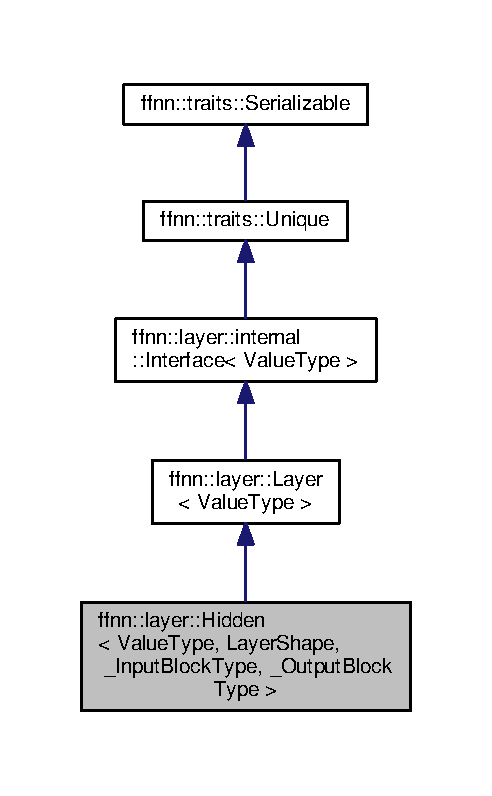
\includegraphics[width=302pt]{classffnn_1_1layer_1_1_hidden__inherit__graph}
\end{center}
\end{figure}


Collaboration diagram for ffnn\-:\-:layer\-:\-:Hidden$<$ Value\-Type, Input\-Height\-At\-Compile\-Time, Input\-Width\-At\-Compile\-Time, Output\-Height\-At\-Compile\-Time, Output\-Width\-At\-Compile\-Time, \-\_\-\-Input\-Block\-Type, \-\_\-\-Output\-Block\-Type, \-\_\-\-Input\-Mapping\-Type, \-\_\-\-Output\-Mapping\-Type $>$\-:\nopagebreak
\begin{figure}[H]
\begin{center}
\leavevmode
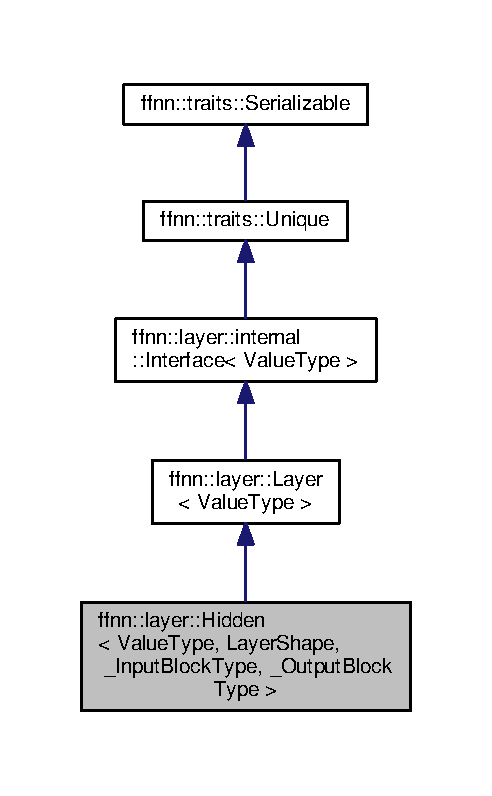
\includegraphics[width=302pt]{classffnn_1_1layer_1_1_hidden__coll__graph}
\end{center}
\end{figure}
\subsection*{Public Types}
\begin{DoxyCompactItemize}
\item 
using \hyperlink{classffnn_1_1layer_1_1_hidden_ac51b180aa7de47794148e32616f0441f}{Base} = \hyperlink{classffnn_1_1layer_1_1_layer}{Layer}$<$ Value\-Type $>$
\begin{DoxyCompactList}\small\item\em Base type alias. \end{DoxyCompactList}\item 
typedef \hyperlink{classffnn_1_1layer_1_1_layer_aeccac281d4220fab9cebf78b004c09d1}{Base\-::\-Size\-Type} \hyperlink{classffnn_1_1layer_1_1_hidden_a3deb1dc4b3a83b3d6749474debee025f}{Size\-Type}
\begin{DoxyCompactList}\small\item\em Size type standardization. \end{DoxyCompactList}\item 
typedef \hyperlink{classffnn_1_1layer_1_1_layer_a0e35ffd6e0657856f3a75323b2db9fcb}{Base\-::\-Offset\-Type} \hyperlink{classffnn_1_1layer_1_1_hidden_a4a191bc002b2545231a3d80c99004693}{Offset\-Type}
\begin{DoxyCompactList}\small\item\em Offset type standardization. \end{DoxyCompactList}\item 
typedef \hyperlink{classffnn_1_1layer_1_1_layer_a104a0f51427df4e03f4ac9e1ce7f6083}{Base\-::\-Dim\-Type} \hyperlink{classffnn_1_1layer_1_1_hidden_aba8b203c8b193a53d19fc26c10b14872}{Dim\-Type}
\begin{DoxyCompactList}\small\item\em Dimension type standardization. \end{DoxyCompactList}\item 
typedef \-\_\-\-Input\-Block\-Type \hyperlink{classffnn_1_1layer_1_1_hidden_a01b9cc4df01a7b26423dcd3a0af17b1c}{Input\-Block\-Type}
\begin{DoxyCompactList}\small\item\em \hyperlink{classffnn_1_1layer_1_1_input}{Input} block type standardization. \end{DoxyCompactList}\item 
typedef \-\_\-\-Output\-Block\-Type \hyperlink{classffnn_1_1layer_1_1_hidden_abb03ddc71360cc7ebdab03cd4d1553ee}{Output\-Block\-Type}
\begin{DoxyCompactList}\small\item\em Iutpu blockt type standardization. \end{DoxyCompactList}\end{DoxyCompactItemize}
\subsection*{Public Member Functions}
\begin{DoxyCompactItemize}
\item 
\hyperlink{classffnn_1_1layer_1_1_hidden_ade54de529e6aa7fd09b1ca61fea0ccc5}{Hidden} (const \hyperlink{classffnn_1_1layer_1_1_hidden_aba8b203c8b193a53d19fc26c10b14872}{Dim\-Type} \&input\-\_\-dim=\hyperlink{classffnn_1_1layer_1_1_hidden_aba8b203c8b193a53d19fc26c10b14872}{Dim\-Type}(Input\-Height\-At\-Compile\-Time, Input\-Width\-At\-Compile\-Time), const \hyperlink{classffnn_1_1layer_1_1_hidden_aba8b203c8b193a53d19fc26c10b14872}{Dim\-Type} \&output\-\_\-dim=\hyperlink{classffnn_1_1layer_1_1_hidden_aba8b203c8b193a53d19fc26c10b14872}{Dim\-Type}(Output\-Height\-At\-Compile\-Time, Output\-Width\-At\-Compile\-Time))
\begin{DoxyCompactList}\small\item\em Setup constructor. \end{DoxyCompactList}\item 
virtual \hyperlink{classffnn_1_1layer_1_1_hidden_a28d2c1175388ed7e9126b7e0ddd45e14}{$\sim$\-Hidden} ()
\item 
virtual bool \hyperlink{classffnn_1_1layer_1_1_hidden_a3b5458a771fcf2371376049d85afbc92}{initialize} ()
\begin{DoxyCompactList}\small\item\em Initialize the layer. \end{DoxyCompactList}\item 
virtual bool \hyperlink{classffnn_1_1layer_1_1_hidden_aed780b7869487b020c839e5a3ce1d8e6}{forward} ()
\begin{DoxyCompactList}\small\item\em Forward value propagation. \end{DoxyCompactList}\item 
virtual bool \hyperlink{classffnn_1_1layer_1_1_hidden_a939fc9f0c269e63220305d787fbe600c}{backward} ()
\begin{DoxyCompactList}\small\item\em Backward value propagation. \end{DoxyCompactList}\item 
virtual bool \hyperlink{classffnn_1_1layer_1_1_hidden_a63913f14b69485eb0c21e02c09f735d4}{update} ()
\begin{DoxyCompactList}\small\item\em Applies layer weight updates. \end{DoxyCompactList}\end{DoxyCompactItemize}
\subsection*{Protected Member Functions}
\begin{DoxyCompactItemize}
\item 
void \hyperlink{classffnn_1_1layer_1_1_hidden_a98305185267a0f7953f1b53c4bce4cf6}{save} (\hyperlink{classffnn_1_1traits_1_1_serializable_a08d986df75d363fa79506d4f6045cb9f}{Output\-Archive} \&ar, \hyperlink{classffnn_1_1traits_1_1_serializable_a08924b3b7d20cb3cb6eafe517d4f7b30}{Version\-Type} version) const 
\begin{DoxyCompactList}\small\item\em Save serializer. \end{DoxyCompactList}\item 
void \hyperlink{classffnn_1_1layer_1_1_hidden_a696f61b2d9b661b7a8d6bdb3dc32b536}{load} (\hyperlink{classffnn_1_1traits_1_1_serializable_a6e626759259f8f370dd4303b4441a234}{Input\-Archive} \&ar, \hyperlink{classffnn_1_1traits_1_1_serializable_a08924b3b7d20cb3cb6eafe517d4f7b30}{Version\-Type} version)
\begin{DoxyCompactList}\small\item\em Load serializer. \end{DoxyCompactList}\end{DoxyCompactItemize}
\subsection*{Protected Attributes}
\begin{DoxyCompactItemize}
\item 
\-\_\-\-Input\-Mapping\-Type\-::\-Ptr \hyperlink{classffnn_1_1layer_1_1_hidden_a2583fadf189c4a9217ffe0146e8f2d1e}{input\-\_\-}
\begin{DoxyCompactList}\small\item\em Memory-\/mapped input vector. \end{DoxyCompactList}\item 
\-\_\-\-Output\-Mapping\-Type\-::\-Ptr \hyperlink{classffnn_1_1layer_1_1_hidden_a6dcd89d479af9b2a9359b1f723dae995}{output\-\_\-}
\begin{DoxyCompactList}\small\item\em Memory-\/mapped output vector. \end{DoxyCompactList}\item 
\-\_\-\-Input\-Mapping\-Type\-::\-Ptr \hyperlink{classffnn_1_1layer_1_1_hidden_aa9ed4266924e9b9da7faf9d53380a3e5}{backward\-\_\-error\-\_\-}
\begin{DoxyCompactList}\small\item\em Backward error vector. \end{DoxyCompactList}\item 
\-\_\-\-Output\-Mapping\-Type\-::\-Ptr \hyperlink{classffnn_1_1layer_1_1_hidden_a9ca7423a16607df0a278002c249e9d1b}{forward\-\_\-error\-\_\-}
\begin{DoxyCompactList}\small\item\em Output-\/target error vector. \end{DoxyCompactList}\end{DoxyCompactItemize}


\subsection{Detailed Description}
\subsubsection*{template$<$typename Value\-Type, F\-F\-N\-N\-\_\-\-S\-I\-Z\-E\-\_\-\-T\-Y\-P\-E Input\-Height\-At\-Compile\-Time = Eigen\-::\-Dynamic, F\-F\-N\-N\-\_\-\-S\-I\-Z\-E\-\_\-\-T\-Y\-P\-E Input\-Width\-At\-Compile\-Time = Eigen\-::\-Dynamic, F\-F\-N\-N\-\_\-\-S\-I\-Z\-E\-\_\-\-T\-Y\-P\-E Output\-Height\-At\-Compile\-Time = Eigen\-::\-Dynamic, F\-F\-N\-N\-\_\-\-S\-I\-Z\-E\-\_\-\-T\-Y\-P\-E Output\-Width\-At\-Compile\-Time = Eigen\-::\-Dynamic, typename \-\_\-\-Input\-Block\-Type = Eigen\-::\-Matrix$<$\-Value\-Type, Input\-Height\-At\-Compile\-Time, Input\-Width\-At\-Compile\-Time, Eigen\-::\-Col\-Major$>$, typename \-\_\-\-Output\-Block\-Type = Eigen\-::\-Matrix$<$\-Value\-Type, Output\-Height\-At\-Compile\-Time, Output\-Width\-At\-Compile\-Time, Eigen\-::\-Col\-Major$>$, typename \-\_\-\-Input\-Mapping\-Type = aligned\-::\-Map$<$\-\_\-\-Input\-Block\-Type$>$, typename \-\_\-\-Output\-Mapping\-Type = aligned\-::\-Map$<$\-\_\-\-Output\-Block\-Type$>$$>$class ffnn\-::layer\-::\-Hidden$<$ Value\-Type, Input\-Height\-At\-Compile\-Time, Input\-Width\-At\-Compile\-Time, Output\-Height\-At\-Compile\-Time, Output\-Width\-At\-Compile\-Time, \-\_\-\-Input\-Block\-Type, \-\_\-\-Output\-Block\-Type, \-\_\-\-Input\-Mapping\-Type, \-\_\-\-Output\-Mapping\-Type $>$}

A network hidden-\/layer object. 

\subsection{Member Typedef Documentation}
\hypertarget{classffnn_1_1layer_1_1_hidden_ac51b180aa7de47794148e32616f0441f}{\index{ffnn\-::layer\-::\-Hidden@{ffnn\-::layer\-::\-Hidden}!Base@{Base}}
\index{Base@{Base}!ffnn::layer::Hidden@{ffnn\-::layer\-::\-Hidden}}
\subsubsection[{Base}]{\setlength{\rightskip}{0pt plus 5cm}template$<$typename Value\-Type, F\-F\-N\-N\-\_\-\-S\-I\-Z\-E\-\_\-\-T\-Y\-P\-E Input\-Height\-At\-Compile\-Time = Eigen\-::\-Dynamic, F\-F\-N\-N\-\_\-\-S\-I\-Z\-E\-\_\-\-T\-Y\-P\-E Input\-Width\-At\-Compile\-Time = Eigen\-::\-Dynamic, F\-F\-N\-N\-\_\-\-S\-I\-Z\-E\-\_\-\-T\-Y\-P\-E Output\-Height\-At\-Compile\-Time = Eigen\-::\-Dynamic, F\-F\-N\-N\-\_\-\-S\-I\-Z\-E\-\_\-\-T\-Y\-P\-E Output\-Width\-At\-Compile\-Time = Eigen\-::\-Dynamic, typename \-\_\-\-Input\-Block\-Type = Eigen\-::\-Matrix$<$\-Value\-Type, Input\-Height\-At\-Compile\-Time, Input\-Width\-At\-Compile\-Time, Eigen\-::\-Col\-Major$>$, typename \-\_\-\-Output\-Block\-Type = Eigen\-::\-Matrix$<$\-Value\-Type, Output\-Height\-At\-Compile\-Time, Output\-Width\-At\-Compile\-Time, Eigen\-::\-Col\-Major$>$, typename \-\_\-\-Input\-Mapping\-Type = aligned\-::\-Map$<$\-\_\-\-Input\-Block\-Type$>$, typename \-\_\-\-Output\-Mapping\-Type = aligned\-::\-Map$<$\-\_\-\-Output\-Block\-Type$>$$>$ using {\bf ffnn\-::layer\-::\-Hidden}$<$ Value\-Type, Input\-Height\-At\-Compile\-Time, Input\-Width\-At\-Compile\-Time, Output\-Height\-At\-Compile\-Time, Output\-Width\-At\-Compile\-Time, \-\_\-\-Input\-Block\-Type, \-\_\-\-Output\-Block\-Type, \-\_\-\-Input\-Mapping\-Type, \-\_\-\-Output\-Mapping\-Type $>$\-::{\bf Base} =  {\bf Layer}$<$Value\-Type$>$}}\label{classffnn_1_1layer_1_1_hidden_ac51b180aa7de47794148e32616f0441f}


Base type alias. 

\hypertarget{classffnn_1_1layer_1_1_hidden_aba8b203c8b193a53d19fc26c10b14872}{\index{ffnn\-::layer\-::\-Hidden@{ffnn\-::layer\-::\-Hidden}!Dim\-Type@{Dim\-Type}}
\index{Dim\-Type@{Dim\-Type}!ffnn::layer::Hidden@{ffnn\-::layer\-::\-Hidden}}
\subsubsection[{Dim\-Type}]{\setlength{\rightskip}{0pt plus 5cm}template$<$typename Value\-Type, F\-F\-N\-N\-\_\-\-S\-I\-Z\-E\-\_\-\-T\-Y\-P\-E Input\-Height\-At\-Compile\-Time = Eigen\-::\-Dynamic, F\-F\-N\-N\-\_\-\-S\-I\-Z\-E\-\_\-\-T\-Y\-P\-E Input\-Width\-At\-Compile\-Time = Eigen\-::\-Dynamic, F\-F\-N\-N\-\_\-\-S\-I\-Z\-E\-\_\-\-T\-Y\-P\-E Output\-Height\-At\-Compile\-Time = Eigen\-::\-Dynamic, F\-F\-N\-N\-\_\-\-S\-I\-Z\-E\-\_\-\-T\-Y\-P\-E Output\-Width\-At\-Compile\-Time = Eigen\-::\-Dynamic, typename \-\_\-\-Input\-Block\-Type = Eigen\-::\-Matrix$<$\-Value\-Type, Input\-Height\-At\-Compile\-Time, Input\-Width\-At\-Compile\-Time, Eigen\-::\-Col\-Major$>$, typename \-\_\-\-Output\-Block\-Type = Eigen\-::\-Matrix$<$\-Value\-Type, Output\-Height\-At\-Compile\-Time, Output\-Width\-At\-Compile\-Time, Eigen\-::\-Col\-Major$>$, typename \-\_\-\-Input\-Mapping\-Type = aligned\-::\-Map$<$\-\_\-\-Input\-Block\-Type$>$, typename \-\_\-\-Output\-Mapping\-Type = aligned\-::\-Map$<$\-\_\-\-Output\-Block\-Type$>$$>$ typedef {\bf Base\-::\-Dim\-Type} {\bf ffnn\-::layer\-::\-Hidden}$<$ Value\-Type, Input\-Height\-At\-Compile\-Time, Input\-Width\-At\-Compile\-Time, Output\-Height\-At\-Compile\-Time, Output\-Width\-At\-Compile\-Time, \-\_\-\-Input\-Block\-Type, \-\_\-\-Output\-Block\-Type, \-\_\-\-Input\-Mapping\-Type, \-\_\-\-Output\-Mapping\-Type $>$\-::{\bf Dim\-Type}}}\label{classffnn_1_1layer_1_1_hidden_aba8b203c8b193a53d19fc26c10b14872}


Dimension type standardization. 

\hypertarget{classffnn_1_1layer_1_1_hidden_a01b9cc4df01a7b26423dcd3a0af17b1c}{\index{ffnn\-::layer\-::\-Hidden@{ffnn\-::layer\-::\-Hidden}!Input\-Block\-Type@{Input\-Block\-Type}}
\index{Input\-Block\-Type@{Input\-Block\-Type}!ffnn::layer::Hidden@{ffnn\-::layer\-::\-Hidden}}
\subsubsection[{Input\-Block\-Type}]{\setlength{\rightskip}{0pt plus 5cm}template$<$typename Value\-Type, F\-F\-N\-N\-\_\-\-S\-I\-Z\-E\-\_\-\-T\-Y\-P\-E Input\-Height\-At\-Compile\-Time = Eigen\-::\-Dynamic, F\-F\-N\-N\-\_\-\-S\-I\-Z\-E\-\_\-\-T\-Y\-P\-E Input\-Width\-At\-Compile\-Time = Eigen\-::\-Dynamic, F\-F\-N\-N\-\_\-\-S\-I\-Z\-E\-\_\-\-T\-Y\-P\-E Output\-Height\-At\-Compile\-Time = Eigen\-::\-Dynamic, F\-F\-N\-N\-\_\-\-S\-I\-Z\-E\-\_\-\-T\-Y\-P\-E Output\-Width\-At\-Compile\-Time = Eigen\-::\-Dynamic, typename \-\_\-\-Input\-Block\-Type = Eigen\-::\-Matrix$<$\-Value\-Type, Input\-Height\-At\-Compile\-Time, Input\-Width\-At\-Compile\-Time, Eigen\-::\-Col\-Major$>$, typename \-\_\-\-Output\-Block\-Type = Eigen\-::\-Matrix$<$\-Value\-Type, Output\-Height\-At\-Compile\-Time, Output\-Width\-At\-Compile\-Time, Eigen\-::\-Col\-Major$>$, typename \-\_\-\-Input\-Mapping\-Type = aligned\-::\-Map$<$\-\_\-\-Input\-Block\-Type$>$, typename \-\_\-\-Output\-Mapping\-Type = aligned\-::\-Map$<$\-\_\-\-Output\-Block\-Type$>$$>$ typedef \-\_\-\-Input\-Block\-Type {\bf ffnn\-::layer\-::\-Hidden}$<$ Value\-Type, Input\-Height\-At\-Compile\-Time, Input\-Width\-At\-Compile\-Time, Output\-Height\-At\-Compile\-Time, Output\-Width\-At\-Compile\-Time, \-\_\-\-Input\-Block\-Type, \-\_\-\-Output\-Block\-Type, \-\_\-\-Input\-Mapping\-Type, \-\_\-\-Output\-Mapping\-Type $>$\-::{\bf Input\-Block\-Type}}}\label{classffnn_1_1layer_1_1_hidden_a01b9cc4df01a7b26423dcd3a0af17b1c}


\hyperlink{classffnn_1_1layer_1_1_input}{Input} block type standardization. 

\hypertarget{classffnn_1_1layer_1_1_hidden_a4a191bc002b2545231a3d80c99004693}{\index{ffnn\-::layer\-::\-Hidden@{ffnn\-::layer\-::\-Hidden}!Offset\-Type@{Offset\-Type}}
\index{Offset\-Type@{Offset\-Type}!ffnn::layer::Hidden@{ffnn\-::layer\-::\-Hidden}}
\subsubsection[{Offset\-Type}]{\setlength{\rightskip}{0pt plus 5cm}template$<$typename Value\-Type, F\-F\-N\-N\-\_\-\-S\-I\-Z\-E\-\_\-\-T\-Y\-P\-E Input\-Height\-At\-Compile\-Time = Eigen\-::\-Dynamic, F\-F\-N\-N\-\_\-\-S\-I\-Z\-E\-\_\-\-T\-Y\-P\-E Input\-Width\-At\-Compile\-Time = Eigen\-::\-Dynamic, F\-F\-N\-N\-\_\-\-S\-I\-Z\-E\-\_\-\-T\-Y\-P\-E Output\-Height\-At\-Compile\-Time = Eigen\-::\-Dynamic, F\-F\-N\-N\-\_\-\-S\-I\-Z\-E\-\_\-\-T\-Y\-P\-E Output\-Width\-At\-Compile\-Time = Eigen\-::\-Dynamic, typename \-\_\-\-Input\-Block\-Type = Eigen\-::\-Matrix$<$\-Value\-Type, Input\-Height\-At\-Compile\-Time, Input\-Width\-At\-Compile\-Time, Eigen\-::\-Col\-Major$>$, typename \-\_\-\-Output\-Block\-Type = Eigen\-::\-Matrix$<$\-Value\-Type, Output\-Height\-At\-Compile\-Time, Output\-Width\-At\-Compile\-Time, Eigen\-::\-Col\-Major$>$, typename \-\_\-\-Input\-Mapping\-Type = aligned\-::\-Map$<$\-\_\-\-Input\-Block\-Type$>$, typename \-\_\-\-Output\-Mapping\-Type = aligned\-::\-Map$<$\-\_\-\-Output\-Block\-Type$>$$>$ typedef {\bf Base\-::\-Offset\-Type} {\bf ffnn\-::layer\-::\-Hidden}$<$ Value\-Type, Input\-Height\-At\-Compile\-Time, Input\-Width\-At\-Compile\-Time, Output\-Height\-At\-Compile\-Time, Output\-Width\-At\-Compile\-Time, \-\_\-\-Input\-Block\-Type, \-\_\-\-Output\-Block\-Type, \-\_\-\-Input\-Mapping\-Type, \-\_\-\-Output\-Mapping\-Type $>$\-::{\bf Offset\-Type}}}\label{classffnn_1_1layer_1_1_hidden_a4a191bc002b2545231a3d80c99004693}


Offset type standardization. 

\hypertarget{classffnn_1_1layer_1_1_hidden_abb03ddc71360cc7ebdab03cd4d1553ee}{\index{ffnn\-::layer\-::\-Hidden@{ffnn\-::layer\-::\-Hidden}!Output\-Block\-Type@{Output\-Block\-Type}}
\index{Output\-Block\-Type@{Output\-Block\-Type}!ffnn::layer::Hidden@{ffnn\-::layer\-::\-Hidden}}
\subsubsection[{Output\-Block\-Type}]{\setlength{\rightskip}{0pt plus 5cm}template$<$typename Value\-Type, F\-F\-N\-N\-\_\-\-S\-I\-Z\-E\-\_\-\-T\-Y\-P\-E Input\-Height\-At\-Compile\-Time = Eigen\-::\-Dynamic, F\-F\-N\-N\-\_\-\-S\-I\-Z\-E\-\_\-\-T\-Y\-P\-E Input\-Width\-At\-Compile\-Time = Eigen\-::\-Dynamic, F\-F\-N\-N\-\_\-\-S\-I\-Z\-E\-\_\-\-T\-Y\-P\-E Output\-Height\-At\-Compile\-Time = Eigen\-::\-Dynamic, F\-F\-N\-N\-\_\-\-S\-I\-Z\-E\-\_\-\-T\-Y\-P\-E Output\-Width\-At\-Compile\-Time = Eigen\-::\-Dynamic, typename \-\_\-\-Input\-Block\-Type = Eigen\-::\-Matrix$<$\-Value\-Type, Input\-Height\-At\-Compile\-Time, Input\-Width\-At\-Compile\-Time, Eigen\-::\-Col\-Major$>$, typename \-\_\-\-Output\-Block\-Type = Eigen\-::\-Matrix$<$\-Value\-Type, Output\-Height\-At\-Compile\-Time, Output\-Width\-At\-Compile\-Time, Eigen\-::\-Col\-Major$>$, typename \-\_\-\-Input\-Mapping\-Type = aligned\-::\-Map$<$\-\_\-\-Input\-Block\-Type$>$, typename \-\_\-\-Output\-Mapping\-Type = aligned\-::\-Map$<$\-\_\-\-Output\-Block\-Type$>$$>$ typedef \-\_\-\-Output\-Block\-Type {\bf ffnn\-::layer\-::\-Hidden}$<$ Value\-Type, Input\-Height\-At\-Compile\-Time, Input\-Width\-At\-Compile\-Time, Output\-Height\-At\-Compile\-Time, Output\-Width\-At\-Compile\-Time, \-\_\-\-Input\-Block\-Type, \-\_\-\-Output\-Block\-Type, \-\_\-\-Input\-Mapping\-Type, \-\_\-\-Output\-Mapping\-Type $>$\-::{\bf Output\-Block\-Type}}}\label{classffnn_1_1layer_1_1_hidden_abb03ddc71360cc7ebdab03cd4d1553ee}


Iutpu blockt type standardization. 

\hypertarget{classffnn_1_1layer_1_1_hidden_a3deb1dc4b3a83b3d6749474debee025f}{\index{ffnn\-::layer\-::\-Hidden@{ffnn\-::layer\-::\-Hidden}!Size\-Type@{Size\-Type}}
\index{Size\-Type@{Size\-Type}!ffnn::layer::Hidden@{ffnn\-::layer\-::\-Hidden}}
\subsubsection[{Size\-Type}]{\setlength{\rightskip}{0pt plus 5cm}template$<$typename Value\-Type, F\-F\-N\-N\-\_\-\-S\-I\-Z\-E\-\_\-\-T\-Y\-P\-E Input\-Height\-At\-Compile\-Time = Eigen\-::\-Dynamic, F\-F\-N\-N\-\_\-\-S\-I\-Z\-E\-\_\-\-T\-Y\-P\-E Input\-Width\-At\-Compile\-Time = Eigen\-::\-Dynamic, F\-F\-N\-N\-\_\-\-S\-I\-Z\-E\-\_\-\-T\-Y\-P\-E Output\-Height\-At\-Compile\-Time = Eigen\-::\-Dynamic, F\-F\-N\-N\-\_\-\-S\-I\-Z\-E\-\_\-\-T\-Y\-P\-E Output\-Width\-At\-Compile\-Time = Eigen\-::\-Dynamic, typename \-\_\-\-Input\-Block\-Type = Eigen\-::\-Matrix$<$\-Value\-Type, Input\-Height\-At\-Compile\-Time, Input\-Width\-At\-Compile\-Time, Eigen\-::\-Col\-Major$>$, typename \-\_\-\-Output\-Block\-Type = Eigen\-::\-Matrix$<$\-Value\-Type, Output\-Height\-At\-Compile\-Time, Output\-Width\-At\-Compile\-Time, Eigen\-::\-Col\-Major$>$, typename \-\_\-\-Input\-Mapping\-Type = aligned\-::\-Map$<$\-\_\-\-Input\-Block\-Type$>$, typename \-\_\-\-Output\-Mapping\-Type = aligned\-::\-Map$<$\-\_\-\-Output\-Block\-Type$>$$>$ typedef {\bf Base\-::\-Size\-Type} {\bf ffnn\-::layer\-::\-Hidden}$<$ Value\-Type, Input\-Height\-At\-Compile\-Time, Input\-Width\-At\-Compile\-Time, Output\-Height\-At\-Compile\-Time, Output\-Width\-At\-Compile\-Time, \-\_\-\-Input\-Block\-Type, \-\_\-\-Output\-Block\-Type, \-\_\-\-Input\-Mapping\-Type, \-\_\-\-Output\-Mapping\-Type $>$\-::{\bf Size\-Type}}}\label{classffnn_1_1layer_1_1_hidden_a3deb1dc4b3a83b3d6749474debee025f}


Size type standardization. 



\subsection{Constructor \& Destructor Documentation}
\hypertarget{classffnn_1_1layer_1_1_hidden_ade54de529e6aa7fd09b1ca61fea0ccc5}{\index{ffnn\-::layer\-::\-Hidden@{ffnn\-::layer\-::\-Hidden}!Hidden@{Hidden}}
\index{Hidden@{Hidden}!ffnn::layer::Hidden@{ffnn\-::layer\-::\-Hidden}}
\subsubsection[{Hidden}]{\setlength{\rightskip}{0pt plus 5cm}template$<$typename Value\-Type, F\-F\-N\-N\-\_\-\-S\-I\-Z\-E\-\_\-\-T\-Y\-P\-E Input\-Height\-At\-Compile\-Time = Eigen\-::\-Dynamic, F\-F\-N\-N\-\_\-\-S\-I\-Z\-E\-\_\-\-T\-Y\-P\-E Input\-Width\-At\-Compile\-Time = Eigen\-::\-Dynamic, F\-F\-N\-N\-\_\-\-S\-I\-Z\-E\-\_\-\-T\-Y\-P\-E Output\-Height\-At\-Compile\-Time = Eigen\-::\-Dynamic, F\-F\-N\-N\-\_\-\-S\-I\-Z\-E\-\_\-\-T\-Y\-P\-E Output\-Width\-At\-Compile\-Time = Eigen\-::\-Dynamic, typename \-\_\-\-Input\-Block\-Type = Eigen\-::\-Matrix$<$\-Value\-Type, Input\-Height\-At\-Compile\-Time, Input\-Width\-At\-Compile\-Time, Eigen\-::\-Col\-Major$>$, typename \-\_\-\-Output\-Block\-Type = Eigen\-::\-Matrix$<$\-Value\-Type, Output\-Height\-At\-Compile\-Time, Output\-Width\-At\-Compile\-Time, Eigen\-::\-Col\-Major$>$, typename \-\_\-\-Input\-Mapping\-Type = aligned\-::\-Map$<$\-\_\-\-Input\-Block\-Type$>$, typename \-\_\-\-Output\-Mapping\-Type = aligned\-::\-Map$<$\-\_\-\-Output\-Block\-Type$>$$>$ {\bf ffnn\-::layer\-::\-Hidden}$<$ Value\-Type, Input\-Height\-At\-Compile\-Time, Input\-Width\-At\-Compile\-Time, Output\-Height\-At\-Compile\-Time, Output\-Width\-At\-Compile\-Time, \-\_\-\-Input\-Block\-Type, \-\_\-\-Output\-Block\-Type, \-\_\-\-Input\-Mapping\-Type, \-\_\-\-Output\-Mapping\-Type $>$\-::{\bf Hidden} (
\begin{DoxyParamCaption}
\item[{const {\bf Dim\-Type} \&}]{input\-\_\-dim = {\ttfamily {\bf Dim\-Type}(InputHeightAtCompileTime,~InputWidthAtCompileTime)}, }
\item[{const {\bf Dim\-Type} \&}]{output\-\_\-dim = {\ttfamily {\bf Dim\-Type}(OutputHeightAtCompileTime,~OutputWidthAtCompileTime)}}
\end{DoxyParamCaption}
)\hspace{0.3cm}{\ttfamily [explicit]}}}\label{classffnn_1_1layer_1_1_hidden_ade54de529e6aa7fd09b1ca61fea0ccc5}


Setup constructor. 


\begin{DoxyParams}{Parameters}
{\em input\-\_\-height} & height of the input surface \\
\hline
{\em input\-\_\-width} & width of the input surface \\
\hline
{\em output\-\_\-height} & height of the output surface \\
\hline
{\em output\-\_\-width} & width of the output surface \\
\hline
\end{DoxyParams}
\hypertarget{classffnn_1_1layer_1_1_hidden_a28d2c1175388ed7e9126b7e0ddd45e14}{\index{ffnn\-::layer\-::\-Hidden@{ffnn\-::layer\-::\-Hidden}!$\sim$\-Hidden@{$\sim$\-Hidden}}
\index{$\sim$\-Hidden@{$\sim$\-Hidden}!ffnn::layer::Hidden@{ffnn\-::layer\-::\-Hidden}}
\subsubsection[{$\sim$\-Hidden}]{\setlength{\rightskip}{0pt plus 5cm}template$<$typename Value\-Type, F\-F\-N\-N\-\_\-\-S\-I\-Z\-E\-\_\-\-T\-Y\-P\-E Input\-Height\-At\-Compile\-Time = Eigen\-::\-Dynamic, F\-F\-N\-N\-\_\-\-S\-I\-Z\-E\-\_\-\-T\-Y\-P\-E Input\-Width\-At\-Compile\-Time = Eigen\-::\-Dynamic, F\-F\-N\-N\-\_\-\-S\-I\-Z\-E\-\_\-\-T\-Y\-P\-E Output\-Height\-At\-Compile\-Time = Eigen\-::\-Dynamic, F\-F\-N\-N\-\_\-\-S\-I\-Z\-E\-\_\-\-T\-Y\-P\-E Output\-Width\-At\-Compile\-Time = Eigen\-::\-Dynamic, typename \-\_\-\-Input\-Block\-Type = Eigen\-::\-Matrix$<$\-Value\-Type, Input\-Height\-At\-Compile\-Time, Input\-Width\-At\-Compile\-Time, Eigen\-::\-Col\-Major$>$, typename \-\_\-\-Output\-Block\-Type = Eigen\-::\-Matrix$<$\-Value\-Type, Output\-Height\-At\-Compile\-Time, Output\-Width\-At\-Compile\-Time, Eigen\-::\-Col\-Major$>$, typename \-\_\-\-Input\-Mapping\-Type = aligned\-::\-Map$<$\-\_\-\-Input\-Block\-Type$>$, typename \-\_\-\-Output\-Mapping\-Type = aligned\-::\-Map$<$\-\_\-\-Output\-Block\-Type$>$$>$ virtual {\bf ffnn\-::layer\-::\-Hidden}$<$ Value\-Type, Input\-Height\-At\-Compile\-Time, Input\-Width\-At\-Compile\-Time, Output\-Height\-At\-Compile\-Time, Output\-Width\-At\-Compile\-Time, \-\_\-\-Input\-Block\-Type, \-\_\-\-Output\-Block\-Type, \-\_\-\-Input\-Mapping\-Type, \-\_\-\-Output\-Mapping\-Type $>$\-::$\sim${\bf Hidden} (
\begin{DoxyParamCaption}
{}
\end{DoxyParamCaption}
)\hspace{0.3cm}{\ttfamily [virtual]}}}\label{classffnn_1_1layer_1_1_hidden_a28d2c1175388ed7e9126b7e0ddd45e14}


\subsection{Member Function Documentation}
\hypertarget{classffnn_1_1layer_1_1_hidden_a939fc9f0c269e63220305d787fbe600c}{\index{ffnn\-::layer\-::\-Hidden@{ffnn\-::layer\-::\-Hidden}!backward@{backward}}
\index{backward@{backward}!ffnn::layer::Hidden@{ffnn\-::layer\-::\-Hidden}}
\subsubsection[{backward}]{\setlength{\rightskip}{0pt plus 5cm}template$<$typename Value\-Type, F\-F\-N\-N\-\_\-\-S\-I\-Z\-E\-\_\-\-T\-Y\-P\-E Input\-Height\-At\-Compile\-Time = Eigen\-::\-Dynamic, F\-F\-N\-N\-\_\-\-S\-I\-Z\-E\-\_\-\-T\-Y\-P\-E Input\-Width\-At\-Compile\-Time = Eigen\-::\-Dynamic, F\-F\-N\-N\-\_\-\-S\-I\-Z\-E\-\_\-\-T\-Y\-P\-E Output\-Height\-At\-Compile\-Time = Eigen\-::\-Dynamic, F\-F\-N\-N\-\_\-\-S\-I\-Z\-E\-\_\-\-T\-Y\-P\-E Output\-Width\-At\-Compile\-Time = Eigen\-::\-Dynamic, typename \-\_\-\-Input\-Block\-Type = Eigen\-::\-Matrix$<$\-Value\-Type, Input\-Height\-At\-Compile\-Time, Input\-Width\-At\-Compile\-Time, Eigen\-::\-Col\-Major$>$, typename \-\_\-\-Output\-Block\-Type = Eigen\-::\-Matrix$<$\-Value\-Type, Output\-Height\-At\-Compile\-Time, Output\-Width\-At\-Compile\-Time, Eigen\-::\-Col\-Major$>$, typename \-\_\-\-Input\-Mapping\-Type = aligned\-::\-Map$<$\-\_\-\-Input\-Block\-Type$>$, typename \-\_\-\-Output\-Mapping\-Type = aligned\-::\-Map$<$\-\_\-\-Output\-Block\-Type$>$$>$ virtual bool {\bf ffnn\-::layer\-::\-Hidden}$<$ Value\-Type, Input\-Height\-At\-Compile\-Time, Input\-Width\-At\-Compile\-Time, Output\-Height\-At\-Compile\-Time, Output\-Width\-At\-Compile\-Time, \-\_\-\-Input\-Block\-Type, \-\_\-\-Output\-Block\-Type, \-\_\-\-Input\-Mapping\-Type, \-\_\-\-Output\-Mapping\-Type $>$\-::backward (
\begin{DoxyParamCaption}
{}
\end{DoxyParamCaption}
)\hspace{0.3cm}{\ttfamily [inline]}, {\ttfamily [virtual]}}}\label{classffnn_1_1layer_1_1_hidden_a939fc9f0c269e63220305d787fbe600c}


Backward value propagation. 


\begin{DoxyRetVals}{Return values}
{\em true} & if backward-\/propagation succeeded \\
\hline
{\em false} & otherwise \\
\hline
\end{DoxyRetVals}


Reimplemented from \hyperlink{classffnn_1_1layer_1_1_layer_a59d5f45393a1b0e4673969c65faaae2a}{ffnn\-::layer\-::\-Layer$<$ Value\-Type $>$}.



Reimplemented in \hyperlink{classffnn_1_1layer_1_1_sparsely_connected_a597ea83c83e8f4f64a1fb7f17a1ea015}{ffnn\-::layer\-::\-Sparsely\-Connected$<$ Value\-Type, Inputs\-At\-Compile\-Time, Outputs\-At\-Compile\-Time $>$}, \hyperlink{classffnn_1_1layer_1_1_fully_connected_afd5c1a006cf33a47cb7e2a982fe4cd6d}{ffnn\-::layer\-::\-Fully\-Connected$<$ Value\-Type, Inputs\-At\-Compile\-Time, Outputs\-At\-Compile\-Time $>$}, and \hyperlink{classffnn_1_1layer_1_1_activation_a3c4284245343f2132dd28eaf7ffbed47}{ffnn\-::layer\-::\-Activation$<$ Value\-Type, Neuron\-Type, Size\-At\-Compile\-Time $>$}.

\hypertarget{classffnn_1_1layer_1_1_hidden_aed780b7869487b020c839e5a3ce1d8e6}{\index{ffnn\-::layer\-::\-Hidden@{ffnn\-::layer\-::\-Hidden}!forward@{forward}}
\index{forward@{forward}!ffnn::layer::Hidden@{ffnn\-::layer\-::\-Hidden}}
\subsubsection[{forward}]{\setlength{\rightskip}{0pt plus 5cm}template$<$typename Value\-Type, F\-F\-N\-N\-\_\-\-S\-I\-Z\-E\-\_\-\-T\-Y\-P\-E Input\-Height\-At\-Compile\-Time = Eigen\-::\-Dynamic, F\-F\-N\-N\-\_\-\-S\-I\-Z\-E\-\_\-\-T\-Y\-P\-E Input\-Width\-At\-Compile\-Time = Eigen\-::\-Dynamic, F\-F\-N\-N\-\_\-\-S\-I\-Z\-E\-\_\-\-T\-Y\-P\-E Output\-Height\-At\-Compile\-Time = Eigen\-::\-Dynamic, F\-F\-N\-N\-\_\-\-S\-I\-Z\-E\-\_\-\-T\-Y\-P\-E Output\-Width\-At\-Compile\-Time = Eigen\-::\-Dynamic, typename \-\_\-\-Input\-Block\-Type = Eigen\-::\-Matrix$<$\-Value\-Type, Input\-Height\-At\-Compile\-Time, Input\-Width\-At\-Compile\-Time, Eigen\-::\-Col\-Major$>$, typename \-\_\-\-Output\-Block\-Type = Eigen\-::\-Matrix$<$\-Value\-Type, Output\-Height\-At\-Compile\-Time, Output\-Width\-At\-Compile\-Time, Eigen\-::\-Col\-Major$>$, typename \-\_\-\-Input\-Mapping\-Type = aligned\-::\-Map$<$\-\_\-\-Input\-Block\-Type$>$, typename \-\_\-\-Output\-Mapping\-Type = aligned\-::\-Map$<$\-\_\-\-Output\-Block\-Type$>$$>$ virtual bool {\bf ffnn\-::layer\-::\-Hidden}$<$ Value\-Type, Input\-Height\-At\-Compile\-Time, Input\-Width\-At\-Compile\-Time, Output\-Height\-At\-Compile\-Time, Output\-Width\-At\-Compile\-Time, \-\_\-\-Input\-Block\-Type, \-\_\-\-Output\-Block\-Type, \-\_\-\-Input\-Mapping\-Type, \-\_\-\-Output\-Mapping\-Type $>$\-::forward (
\begin{DoxyParamCaption}
{}
\end{DoxyParamCaption}
)\hspace{0.3cm}{\ttfamily [inline]}, {\ttfamily [virtual]}}}\label{classffnn_1_1layer_1_1_hidden_aed780b7869487b020c839e5a3ce1d8e6}


Forward value propagation. 


\begin{DoxyRetVals}{Return values}
{\em true} & if forward-\/propagation succeeded \\
\hline
{\em false} & otherwise \\
\hline
\end{DoxyRetVals}


Reimplemented from \hyperlink{classffnn_1_1layer_1_1_layer_a832518de9beb442be0764e49ab24d78d}{ffnn\-::layer\-::\-Layer$<$ Value\-Type $>$}.



Reimplemented in \hyperlink{classffnn_1_1layer_1_1_sparsely_connected_a53f1d9a2edfdd2e47164b24121c23acc}{ffnn\-::layer\-::\-Sparsely\-Connected$<$ Value\-Type, Inputs\-At\-Compile\-Time, Outputs\-At\-Compile\-Time $>$}, \hyperlink{classffnn_1_1layer_1_1_fully_connected_ac49087ab2d66019f2d0244c76987fa50}{ffnn\-::layer\-::\-Fully\-Connected$<$ Value\-Type, Inputs\-At\-Compile\-Time, Outputs\-At\-Compile\-Time $>$}, and \hyperlink{classffnn_1_1layer_1_1_activation_aa7f88c8bc20589dc51d9dd615b8c4580}{ffnn\-::layer\-::\-Activation$<$ Value\-Type, Neuron\-Type, Size\-At\-Compile\-Time $>$}.

\hypertarget{classffnn_1_1layer_1_1_hidden_a3b5458a771fcf2371376049d85afbc92}{\index{ffnn\-::layer\-::\-Hidden@{ffnn\-::layer\-::\-Hidden}!initialize@{initialize}}
\index{initialize@{initialize}!ffnn::layer::Hidden@{ffnn\-::layer\-::\-Hidden}}
\subsubsection[{initialize}]{\setlength{\rightskip}{0pt plus 5cm}template$<$typename Value\-Type, F\-F\-N\-N\-\_\-\-S\-I\-Z\-E\-\_\-\-T\-Y\-P\-E Input\-Height\-At\-Compile\-Time = Eigen\-::\-Dynamic, F\-F\-N\-N\-\_\-\-S\-I\-Z\-E\-\_\-\-T\-Y\-P\-E Input\-Width\-At\-Compile\-Time = Eigen\-::\-Dynamic, F\-F\-N\-N\-\_\-\-S\-I\-Z\-E\-\_\-\-T\-Y\-P\-E Output\-Height\-At\-Compile\-Time = Eigen\-::\-Dynamic, F\-F\-N\-N\-\_\-\-S\-I\-Z\-E\-\_\-\-T\-Y\-P\-E Output\-Width\-At\-Compile\-Time = Eigen\-::\-Dynamic, typename \-\_\-\-Input\-Block\-Type = Eigen\-::\-Matrix$<$\-Value\-Type, Input\-Height\-At\-Compile\-Time, Input\-Width\-At\-Compile\-Time, Eigen\-::\-Col\-Major$>$, typename \-\_\-\-Output\-Block\-Type = Eigen\-::\-Matrix$<$\-Value\-Type, Output\-Height\-At\-Compile\-Time, Output\-Width\-At\-Compile\-Time, Eigen\-::\-Col\-Major$>$, typename \-\_\-\-Input\-Mapping\-Type = aligned\-::\-Map$<$\-\_\-\-Input\-Block\-Type$>$, typename \-\_\-\-Output\-Mapping\-Type = aligned\-::\-Map$<$\-\_\-\-Output\-Block\-Type$>$$>$ virtual bool {\bf ffnn\-::layer\-::\-Hidden}$<$ Value\-Type, Input\-Height\-At\-Compile\-Time, Input\-Width\-At\-Compile\-Time, Output\-Height\-At\-Compile\-Time, Output\-Width\-At\-Compile\-Time, \-\_\-\-Input\-Block\-Type, \-\_\-\-Output\-Block\-Type, \-\_\-\-Input\-Mapping\-Type, \-\_\-\-Output\-Mapping\-Type $>$\-::initialize (
\begin{DoxyParamCaption}
{}
\end{DoxyParamCaption}
)\hspace{0.3cm}{\ttfamily [virtual]}}}\label{classffnn_1_1layer_1_1_hidden_a3b5458a771fcf2371376049d85afbc92}


Initialize the layer. 



Reimplemented from \hyperlink{classffnn_1_1layer_1_1_layer_ae8a7daa81382a7965b8ab8861da7e522}{ffnn\-::layer\-::\-Layer$<$ Value\-Type $>$}.



Reimplemented in \hyperlink{classffnn_1_1layer_1_1_convolution_a158af9a753113ac55730abd7b56b8684}{ffnn\-::layer\-::\-Convolution$<$ Value\-Type, Height\-At\-Compile\-Time, Width\-At\-Compile\-Time, Depth\-At\-Compile\-Time, Filter\-Height\-At\-Compile\-Time, Filter\-Width\-At\-Compile\-Time, Filter\-Count\-At\-Compile\-Time, Stride, Embedding\-Mode $>$}, \hyperlink{classffnn_1_1layer_1_1_sparsely_connected_abb2966b5e7813c43ae2ea5448188a9fb}{ffnn\-::layer\-::\-Sparsely\-Connected$<$ Value\-Type, Inputs\-At\-Compile\-Time, Outputs\-At\-Compile\-Time $>$}, \hyperlink{classffnn_1_1layer_1_1_fully_connected_aec414194202f845b866b0e8b2a51235c}{ffnn\-::layer\-::\-Fully\-Connected$<$ Value\-Type, Inputs\-At\-Compile\-Time, Outputs\-At\-Compile\-Time $>$}, and \hyperlink{classffnn_1_1layer_1_1_activation_ae73ef2d36d9c5ce3c219f6a51cba3c35}{ffnn\-::layer\-::\-Activation$<$ Value\-Type, Neuron\-Type, Size\-At\-Compile\-Time $>$}.

\hypertarget{classffnn_1_1layer_1_1_hidden_a696f61b2d9b661b7a8d6bdb3dc32b536}{\index{ffnn\-::layer\-::\-Hidden@{ffnn\-::layer\-::\-Hidden}!load@{load}}
\index{load@{load}!ffnn::layer::Hidden@{ffnn\-::layer\-::\-Hidden}}
\subsubsection[{load}]{\setlength{\rightskip}{0pt plus 5cm}template$<$typename Value\-Type, F\-F\-N\-N\-\_\-\-S\-I\-Z\-E\-\_\-\-T\-Y\-P\-E Input\-Height\-At\-Compile\-Time = Eigen\-::\-Dynamic, F\-F\-N\-N\-\_\-\-S\-I\-Z\-E\-\_\-\-T\-Y\-P\-E Input\-Width\-At\-Compile\-Time = Eigen\-::\-Dynamic, F\-F\-N\-N\-\_\-\-S\-I\-Z\-E\-\_\-\-T\-Y\-P\-E Output\-Height\-At\-Compile\-Time = Eigen\-::\-Dynamic, F\-F\-N\-N\-\_\-\-S\-I\-Z\-E\-\_\-\-T\-Y\-P\-E Output\-Width\-At\-Compile\-Time = Eigen\-::\-Dynamic, typename \-\_\-\-Input\-Block\-Type = Eigen\-::\-Matrix$<$\-Value\-Type, Input\-Height\-At\-Compile\-Time, Input\-Width\-At\-Compile\-Time, Eigen\-::\-Col\-Major$>$, typename \-\_\-\-Output\-Block\-Type = Eigen\-::\-Matrix$<$\-Value\-Type, Output\-Height\-At\-Compile\-Time, Output\-Width\-At\-Compile\-Time, Eigen\-::\-Col\-Major$>$, typename \-\_\-\-Input\-Mapping\-Type = aligned\-::\-Map$<$\-\_\-\-Input\-Block\-Type$>$, typename \-\_\-\-Output\-Mapping\-Type = aligned\-::\-Map$<$\-\_\-\-Output\-Block\-Type$>$$>$ void {\bf ffnn\-::layer\-::\-Hidden}$<$ Value\-Type, Input\-Height\-At\-Compile\-Time, Input\-Width\-At\-Compile\-Time, Output\-Height\-At\-Compile\-Time, Output\-Width\-At\-Compile\-Time, \-\_\-\-Input\-Block\-Type, \-\_\-\-Output\-Block\-Type, \-\_\-\-Input\-Mapping\-Type, \-\_\-\-Output\-Mapping\-Type $>$\-::load (
\begin{DoxyParamCaption}
\item[{{\bf Input\-Archive} \&}]{ar, }
\item[{{\bf Version\-Type}}]{version}
\end{DoxyParamCaption}
)\hspace{0.3cm}{\ttfamily [protected]}, {\ttfamily [virtual]}}}\label{classffnn_1_1layer_1_1_hidden_a696f61b2d9b661b7a8d6bdb3dc32b536}


Load serializer. 



Reimplemented from \hyperlink{classffnn_1_1traits_1_1_unique_af1e937c2908ed2ff707d6a7d1b5b13d2}{ffnn\-::traits\-::\-Unique}.

\hypertarget{classffnn_1_1layer_1_1_hidden_a98305185267a0f7953f1b53c4bce4cf6}{\index{ffnn\-::layer\-::\-Hidden@{ffnn\-::layer\-::\-Hidden}!save@{save}}
\index{save@{save}!ffnn::layer::Hidden@{ffnn\-::layer\-::\-Hidden}}
\subsubsection[{save}]{\setlength{\rightskip}{0pt plus 5cm}template$<$typename Value\-Type, F\-F\-N\-N\-\_\-\-S\-I\-Z\-E\-\_\-\-T\-Y\-P\-E Input\-Height\-At\-Compile\-Time = Eigen\-::\-Dynamic, F\-F\-N\-N\-\_\-\-S\-I\-Z\-E\-\_\-\-T\-Y\-P\-E Input\-Width\-At\-Compile\-Time = Eigen\-::\-Dynamic, F\-F\-N\-N\-\_\-\-S\-I\-Z\-E\-\_\-\-T\-Y\-P\-E Output\-Height\-At\-Compile\-Time = Eigen\-::\-Dynamic, F\-F\-N\-N\-\_\-\-S\-I\-Z\-E\-\_\-\-T\-Y\-P\-E Output\-Width\-At\-Compile\-Time = Eigen\-::\-Dynamic, typename \-\_\-\-Input\-Block\-Type = Eigen\-::\-Matrix$<$\-Value\-Type, Input\-Height\-At\-Compile\-Time, Input\-Width\-At\-Compile\-Time, Eigen\-::\-Col\-Major$>$, typename \-\_\-\-Output\-Block\-Type = Eigen\-::\-Matrix$<$\-Value\-Type, Output\-Height\-At\-Compile\-Time, Output\-Width\-At\-Compile\-Time, Eigen\-::\-Col\-Major$>$, typename \-\_\-\-Input\-Mapping\-Type = aligned\-::\-Map$<$\-\_\-\-Input\-Block\-Type$>$, typename \-\_\-\-Output\-Mapping\-Type = aligned\-::\-Map$<$\-\_\-\-Output\-Block\-Type$>$$>$ void {\bf ffnn\-::layer\-::\-Hidden}$<$ Value\-Type, Input\-Height\-At\-Compile\-Time, Input\-Width\-At\-Compile\-Time, Output\-Height\-At\-Compile\-Time, Output\-Width\-At\-Compile\-Time, \-\_\-\-Input\-Block\-Type, \-\_\-\-Output\-Block\-Type, \-\_\-\-Input\-Mapping\-Type, \-\_\-\-Output\-Mapping\-Type $>$\-::save (
\begin{DoxyParamCaption}
\item[{{\bf Output\-Archive} \&}]{ar, }
\item[{{\bf Version\-Type}}]{version}
\end{DoxyParamCaption}
) const\hspace{0.3cm}{\ttfamily [protected]}, {\ttfamily [virtual]}}}\label{classffnn_1_1layer_1_1_hidden_a98305185267a0f7953f1b53c4bce4cf6}


Save serializer. 



Reimplemented from \hyperlink{classffnn_1_1traits_1_1_unique_ad8be6fcb9a7519603b2aab19b3c6d593}{ffnn\-::traits\-::\-Unique}.

\hypertarget{classffnn_1_1layer_1_1_hidden_a63913f14b69485eb0c21e02c09f735d4}{\index{ffnn\-::layer\-::\-Hidden@{ffnn\-::layer\-::\-Hidden}!update@{update}}
\index{update@{update}!ffnn::layer::Hidden@{ffnn\-::layer\-::\-Hidden}}
\subsubsection[{update}]{\setlength{\rightskip}{0pt plus 5cm}template$<$typename Value\-Type, F\-F\-N\-N\-\_\-\-S\-I\-Z\-E\-\_\-\-T\-Y\-P\-E Input\-Height\-At\-Compile\-Time = Eigen\-::\-Dynamic, F\-F\-N\-N\-\_\-\-S\-I\-Z\-E\-\_\-\-T\-Y\-P\-E Input\-Width\-At\-Compile\-Time = Eigen\-::\-Dynamic, F\-F\-N\-N\-\_\-\-S\-I\-Z\-E\-\_\-\-T\-Y\-P\-E Output\-Height\-At\-Compile\-Time = Eigen\-::\-Dynamic, F\-F\-N\-N\-\_\-\-S\-I\-Z\-E\-\_\-\-T\-Y\-P\-E Output\-Width\-At\-Compile\-Time = Eigen\-::\-Dynamic, typename \-\_\-\-Input\-Block\-Type = Eigen\-::\-Matrix$<$\-Value\-Type, Input\-Height\-At\-Compile\-Time, Input\-Width\-At\-Compile\-Time, Eigen\-::\-Col\-Major$>$, typename \-\_\-\-Output\-Block\-Type = Eigen\-::\-Matrix$<$\-Value\-Type, Output\-Height\-At\-Compile\-Time, Output\-Width\-At\-Compile\-Time, Eigen\-::\-Col\-Major$>$, typename \-\_\-\-Input\-Mapping\-Type = aligned\-::\-Map$<$\-\_\-\-Input\-Block\-Type$>$, typename \-\_\-\-Output\-Mapping\-Type = aligned\-::\-Map$<$\-\_\-\-Output\-Block\-Type$>$$>$ virtual bool {\bf ffnn\-::layer\-::\-Hidden}$<$ Value\-Type, Input\-Height\-At\-Compile\-Time, Input\-Width\-At\-Compile\-Time, Output\-Height\-At\-Compile\-Time, Output\-Width\-At\-Compile\-Time, \-\_\-\-Input\-Block\-Type, \-\_\-\-Output\-Block\-Type, \-\_\-\-Input\-Mapping\-Type, \-\_\-\-Output\-Mapping\-Type $>$\-::update (
\begin{DoxyParamCaption}
{}
\end{DoxyParamCaption}
)\hspace{0.3cm}{\ttfamily [inline]}, {\ttfamily [virtual]}}}\label{classffnn_1_1layer_1_1_hidden_a63913f14b69485eb0c21e02c09f735d4}


Applies layer weight updates. 


\begin{DoxyRetVals}{Return values}
{\em true} & if weight update succeeded \\
\hline
{\em false} & otherwise \\
\hline
\end{DoxyRetVals}


Reimplemented from \hyperlink{classffnn_1_1layer_1_1_layer_a25bf06cfea93baf1c80e21d0a88a5e4a}{ffnn\-::layer\-::\-Layer$<$ Value\-Type $>$}.



Reimplemented in \hyperlink{classffnn_1_1layer_1_1_sparsely_connected_afa564d528e74917231da2d038f76e3f1}{ffnn\-::layer\-::\-Sparsely\-Connected$<$ Value\-Type, Inputs\-At\-Compile\-Time, Outputs\-At\-Compile\-Time $>$}, and \hyperlink{classffnn_1_1layer_1_1_fully_connected_a3194dde96feea7d008cc0c27f30cc805}{ffnn\-::layer\-::\-Fully\-Connected$<$ Value\-Type, Inputs\-At\-Compile\-Time, Outputs\-At\-Compile\-Time $>$}.



\subsection{Member Data Documentation}
\hypertarget{classffnn_1_1layer_1_1_hidden_aa9ed4266924e9b9da7faf9d53380a3e5}{\index{ffnn\-::layer\-::\-Hidden@{ffnn\-::layer\-::\-Hidden}!backward\-\_\-error\-\_\-@{backward\-\_\-error\-\_\-}}
\index{backward\-\_\-error\-\_\-@{backward\-\_\-error\-\_\-}!ffnn::layer::Hidden@{ffnn\-::layer\-::\-Hidden}}
\subsubsection[{backward\-\_\-error\-\_\-}]{\setlength{\rightskip}{0pt plus 5cm}template$<$typename Value\-Type, F\-F\-N\-N\-\_\-\-S\-I\-Z\-E\-\_\-\-T\-Y\-P\-E Input\-Height\-At\-Compile\-Time = Eigen\-::\-Dynamic, F\-F\-N\-N\-\_\-\-S\-I\-Z\-E\-\_\-\-T\-Y\-P\-E Input\-Width\-At\-Compile\-Time = Eigen\-::\-Dynamic, F\-F\-N\-N\-\_\-\-S\-I\-Z\-E\-\_\-\-T\-Y\-P\-E Output\-Height\-At\-Compile\-Time = Eigen\-::\-Dynamic, F\-F\-N\-N\-\_\-\-S\-I\-Z\-E\-\_\-\-T\-Y\-P\-E Output\-Width\-At\-Compile\-Time = Eigen\-::\-Dynamic, typename \-\_\-\-Input\-Block\-Type = Eigen\-::\-Matrix$<$\-Value\-Type, Input\-Height\-At\-Compile\-Time, Input\-Width\-At\-Compile\-Time, Eigen\-::\-Col\-Major$>$, typename \-\_\-\-Output\-Block\-Type = Eigen\-::\-Matrix$<$\-Value\-Type, Output\-Height\-At\-Compile\-Time, Output\-Width\-At\-Compile\-Time, Eigen\-::\-Col\-Major$>$, typename \-\_\-\-Input\-Mapping\-Type = aligned\-::\-Map$<$\-\_\-\-Input\-Block\-Type$>$, typename \-\_\-\-Output\-Mapping\-Type = aligned\-::\-Map$<$\-\_\-\-Output\-Block\-Type$>$$>$ \-\_\-\-Input\-Mapping\-Type\-::\-Ptr {\bf ffnn\-::layer\-::\-Hidden}$<$ Value\-Type, Input\-Height\-At\-Compile\-Time, Input\-Width\-At\-Compile\-Time, Output\-Height\-At\-Compile\-Time, Output\-Width\-At\-Compile\-Time, \-\_\-\-Input\-Block\-Type, \-\_\-\-Output\-Block\-Type, \-\_\-\-Input\-Mapping\-Type, \-\_\-\-Output\-Mapping\-Type $>$\-::backward\-\_\-error\-\_\-\hspace{0.3cm}{\ttfamily [protected]}}}\label{classffnn_1_1layer_1_1_hidden_aa9ed4266924e9b9da7faf9d53380a3e5}


Backward error vector. 



Referenced by ffnn\-::optimizer\-::\-Gradient\-Descent$<$ layer\-::\-Fully\-Connected$<$ Value\-Type, Inputs\-At\-Compile\-Time, Outputs\-At\-Compile\-Time $>$ $>$\-::backward(), and ffnn\-::optimizer\-::\-Gradient\-Descent$<$ layer\-::\-Sparsely\-Connected$<$ Value\-Type, Inputs\-At\-Compile\-Time, Outputs\-At\-Compile\-Time $>$ $>$\-::backward().

\hypertarget{classffnn_1_1layer_1_1_hidden_a9ca7423a16607df0a278002c249e9d1b}{\index{ffnn\-::layer\-::\-Hidden@{ffnn\-::layer\-::\-Hidden}!forward\-\_\-error\-\_\-@{forward\-\_\-error\-\_\-}}
\index{forward\-\_\-error\-\_\-@{forward\-\_\-error\-\_\-}!ffnn::layer::Hidden@{ffnn\-::layer\-::\-Hidden}}
\subsubsection[{forward\-\_\-error\-\_\-}]{\setlength{\rightskip}{0pt plus 5cm}template$<$typename Value\-Type, F\-F\-N\-N\-\_\-\-S\-I\-Z\-E\-\_\-\-T\-Y\-P\-E Input\-Height\-At\-Compile\-Time = Eigen\-::\-Dynamic, F\-F\-N\-N\-\_\-\-S\-I\-Z\-E\-\_\-\-T\-Y\-P\-E Input\-Width\-At\-Compile\-Time = Eigen\-::\-Dynamic, F\-F\-N\-N\-\_\-\-S\-I\-Z\-E\-\_\-\-T\-Y\-P\-E Output\-Height\-At\-Compile\-Time = Eigen\-::\-Dynamic, F\-F\-N\-N\-\_\-\-S\-I\-Z\-E\-\_\-\-T\-Y\-P\-E Output\-Width\-At\-Compile\-Time = Eigen\-::\-Dynamic, typename \-\_\-\-Input\-Block\-Type = Eigen\-::\-Matrix$<$\-Value\-Type, Input\-Height\-At\-Compile\-Time, Input\-Width\-At\-Compile\-Time, Eigen\-::\-Col\-Major$>$, typename \-\_\-\-Output\-Block\-Type = Eigen\-::\-Matrix$<$\-Value\-Type, Output\-Height\-At\-Compile\-Time, Output\-Width\-At\-Compile\-Time, Eigen\-::\-Col\-Major$>$, typename \-\_\-\-Input\-Mapping\-Type = aligned\-::\-Map$<$\-\_\-\-Input\-Block\-Type$>$, typename \-\_\-\-Output\-Mapping\-Type = aligned\-::\-Map$<$\-\_\-\-Output\-Block\-Type$>$$>$ \-\_\-\-Output\-Mapping\-Type\-::\-Ptr {\bf ffnn\-::layer\-::\-Hidden}$<$ Value\-Type, Input\-Height\-At\-Compile\-Time, Input\-Width\-At\-Compile\-Time, Output\-Height\-At\-Compile\-Time, Output\-Width\-At\-Compile\-Time, \-\_\-\-Input\-Block\-Type, \-\_\-\-Output\-Block\-Type, \-\_\-\-Input\-Mapping\-Type, \-\_\-\-Output\-Mapping\-Type $>$\-::forward\-\_\-error\-\_\-\hspace{0.3cm}{\ttfamily [protected]}}}\label{classffnn_1_1layer_1_1_hidden_a9ca7423a16607df0a278002c249e9d1b}


Output-\/target error vector. 



Referenced by ffnn\-::optimizer\-::\-Gradient\-Descent$<$ layer\-::\-Fully\-Connected$<$ Value\-Type, Inputs\-At\-Compile\-Time, Outputs\-At\-Compile\-Time $>$ $>$\-::backward(), and ffnn\-::optimizer\-::\-Gradient\-Descent$<$ layer\-::\-Sparsely\-Connected$<$ Value\-Type, Inputs\-At\-Compile\-Time, Outputs\-At\-Compile\-Time $>$ $>$\-::backward().

\hypertarget{classffnn_1_1layer_1_1_hidden_a2583fadf189c4a9217ffe0146e8f2d1e}{\index{ffnn\-::layer\-::\-Hidden@{ffnn\-::layer\-::\-Hidden}!input\-\_\-@{input\-\_\-}}
\index{input\-\_\-@{input\-\_\-}!ffnn::layer::Hidden@{ffnn\-::layer\-::\-Hidden}}
\subsubsection[{input\-\_\-}]{\setlength{\rightskip}{0pt plus 5cm}template$<$typename Value\-Type, F\-F\-N\-N\-\_\-\-S\-I\-Z\-E\-\_\-\-T\-Y\-P\-E Input\-Height\-At\-Compile\-Time = Eigen\-::\-Dynamic, F\-F\-N\-N\-\_\-\-S\-I\-Z\-E\-\_\-\-T\-Y\-P\-E Input\-Width\-At\-Compile\-Time = Eigen\-::\-Dynamic, F\-F\-N\-N\-\_\-\-S\-I\-Z\-E\-\_\-\-T\-Y\-P\-E Output\-Height\-At\-Compile\-Time = Eigen\-::\-Dynamic, F\-F\-N\-N\-\_\-\-S\-I\-Z\-E\-\_\-\-T\-Y\-P\-E Output\-Width\-At\-Compile\-Time = Eigen\-::\-Dynamic, typename \-\_\-\-Input\-Block\-Type = Eigen\-::\-Matrix$<$\-Value\-Type, Input\-Height\-At\-Compile\-Time, Input\-Width\-At\-Compile\-Time, Eigen\-::\-Col\-Major$>$, typename \-\_\-\-Output\-Block\-Type = Eigen\-::\-Matrix$<$\-Value\-Type, Output\-Height\-At\-Compile\-Time, Output\-Width\-At\-Compile\-Time, Eigen\-::\-Col\-Major$>$, typename \-\_\-\-Input\-Mapping\-Type = aligned\-::\-Map$<$\-\_\-\-Input\-Block\-Type$>$, typename \-\_\-\-Output\-Mapping\-Type = aligned\-::\-Map$<$\-\_\-\-Output\-Block\-Type$>$$>$ \-\_\-\-Input\-Mapping\-Type\-::\-Ptr {\bf ffnn\-::layer\-::\-Hidden}$<$ Value\-Type, Input\-Height\-At\-Compile\-Time, Input\-Width\-At\-Compile\-Time, Output\-Height\-At\-Compile\-Time, Output\-Width\-At\-Compile\-Time, \-\_\-\-Input\-Block\-Type, \-\_\-\-Output\-Block\-Type, \-\_\-\-Input\-Mapping\-Type, \-\_\-\-Output\-Mapping\-Type $>$\-::input\-\_\-\hspace{0.3cm}{\ttfamily [protected]}}}\label{classffnn_1_1layer_1_1_hidden_a2583fadf189c4a9217ffe0146e8f2d1e}


Memory-\/mapped input vector. 



Referenced by ffnn\-::optimizer\-::\-Gradient\-Descent$<$ layer\-::\-Fully\-Connected$<$ Value\-Type, Inputs\-At\-Compile\-Time, Outputs\-At\-Compile\-Time $>$ $>$\-::forward(), and ffnn\-::optimizer\-::\-Gradient\-Descent$<$ layer\-::\-Sparsely\-Connected$<$ Value\-Type, Inputs\-At\-Compile\-Time, Outputs\-At\-Compile\-Time $>$ $>$\-::forward().

\hypertarget{classffnn_1_1layer_1_1_hidden_a6dcd89d479af9b2a9359b1f723dae995}{\index{ffnn\-::layer\-::\-Hidden@{ffnn\-::layer\-::\-Hidden}!output\-\_\-@{output\-\_\-}}
\index{output\-\_\-@{output\-\_\-}!ffnn::layer::Hidden@{ffnn\-::layer\-::\-Hidden}}
\subsubsection[{output\-\_\-}]{\setlength{\rightskip}{0pt plus 5cm}template$<$typename Value\-Type, F\-F\-N\-N\-\_\-\-S\-I\-Z\-E\-\_\-\-T\-Y\-P\-E Input\-Height\-At\-Compile\-Time = Eigen\-::\-Dynamic, F\-F\-N\-N\-\_\-\-S\-I\-Z\-E\-\_\-\-T\-Y\-P\-E Input\-Width\-At\-Compile\-Time = Eigen\-::\-Dynamic, F\-F\-N\-N\-\_\-\-S\-I\-Z\-E\-\_\-\-T\-Y\-P\-E Output\-Height\-At\-Compile\-Time = Eigen\-::\-Dynamic, F\-F\-N\-N\-\_\-\-S\-I\-Z\-E\-\_\-\-T\-Y\-P\-E Output\-Width\-At\-Compile\-Time = Eigen\-::\-Dynamic, typename \-\_\-\-Input\-Block\-Type = Eigen\-::\-Matrix$<$\-Value\-Type, Input\-Height\-At\-Compile\-Time, Input\-Width\-At\-Compile\-Time, Eigen\-::\-Col\-Major$>$, typename \-\_\-\-Output\-Block\-Type = Eigen\-::\-Matrix$<$\-Value\-Type, Output\-Height\-At\-Compile\-Time, Output\-Width\-At\-Compile\-Time, Eigen\-::\-Col\-Major$>$, typename \-\_\-\-Input\-Mapping\-Type = aligned\-::\-Map$<$\-\_\-\-Input\-Block\-Type$>$, typename \-\_\-\-Output\-Mapping\-Type = aligned\-::\-Map$<$\-\_\-\-Output\-Block\-Type$>$$>$ \-\_\-\-Output\-Mapping\-Type\-::\-Ptr {\bf ffnn\-::layer\-::\-Hidden}$<$ Value\-Type, Input\-Height\-At\-Compile\-Time, Input\-Width\-At\-Compile\-Time, Output\-Height\-At\-Compile\-Time, Output\-Width\-At\-Compile\-Time, \-\_\-\-Input\-Block\-Type, \-\_\-\-Output\-Block\-Type, \-\_\-\-Input\-Mapping\-Type, \-\_\-\-Output\-Mapping\-Type $>$\-::output\-\_\-\hspace{0.3cm}{\ttfamily [protected]}}}\label{classffnn_1_1layer_1_1_hidden_a6dcd89d479af9b2a9359b1f723dae995}


Memory-\/mapped output vector. 



The documentation for this class was generated from the following file\-:\begin{DoxyCompactItemize}
\item 
/home/briancairl/packages/src/ffnn-\/cpp/ffnn/include/ffnn/layer/\hyperlink{hidden_8h}{hidden.\-h}\end{DoxyCompactItemize}

\hypertarget{classffnn_1_1layer_1_1_input}{\section{ffnn\-:\-:layer\-:\-:Input$<$ Value\-Type, Network\-Inputs\-At\-Compile\-Time $>$ Class Template Reference}
\label{classffnn_1_1layer_1_1_input}\index{ffnn\-::layer\-::\-Input$<$ Value\-Type, Network\-Inputs\-At\-Compile\-Time $>$@{ffnn\-::layer\-::\-Input$<$ Value\-Type, Network\-Inputs\-At\-Compile\-Time $>$}}
}


A layer which handles network inputs.  




{\ttfamily \#include \char`\"{}input.\-h\char`\"{}}



Inheritance diagram for ffnn\-:\-:layer\-:\-:Input$<$ Value\-Type, Network\-Inputs\-At\-Compile\-Time $>$\-:\nopagebreak
\begin{figure}[H]
\begin{center}
\leavevmode
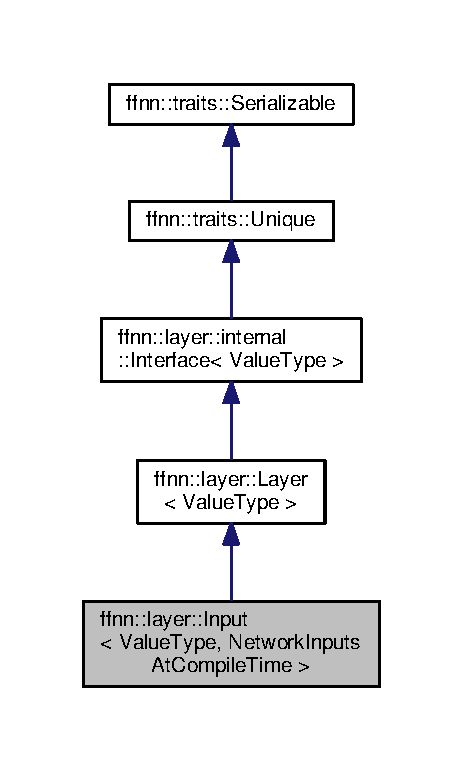
\includegraphics[width=222pt]{classffnn_1_1layer_1_1_input__inherit__graph}
\end{center}
\end{figure}


Collaboration diagram for ffnn\-:\-:layer\-:\-:Input$<$ Value\-Type, Network\-Inputs\-At\-Compile\-Time $>$\-:\nopagebreak
\begin{figure}[H]
\begin{center}
\leavevmode
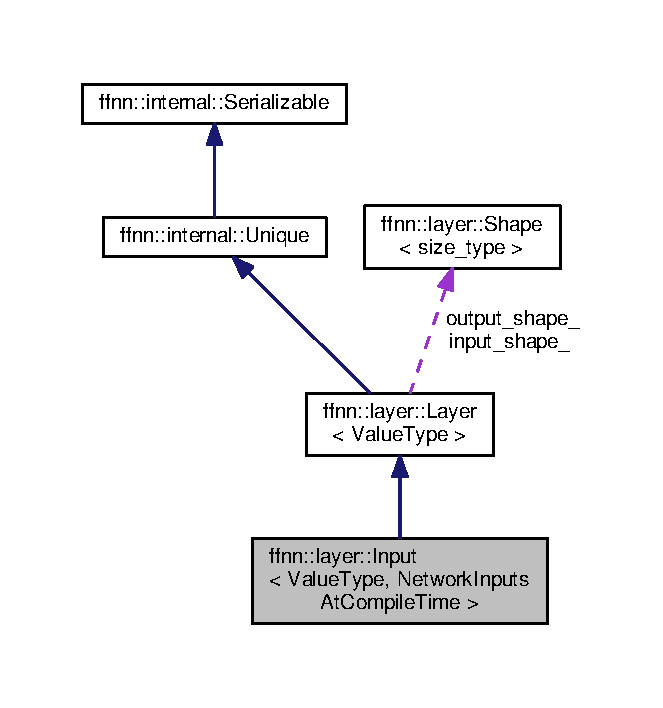
\includegraphics[width=318pt]{classffnn_1_1layer_1_1_input__coll__graph}
\end{center}
\end{figure}
\subsection*{Public Types}
\begin{DoxyCompactItemize}
\item 
using \hyperlink{classffnn_1_1layer_1_1_input_a7d3eef885863ffbab29a2dba5b9d6e2a}{Base} = \hyperlink{classffnn_1_1layer_1_1_layer}{Layer}$<$ Value\-Type $>$
\begin{DoxyCompactList}\small\item\em Base type alias. \end{DoxyCompactList}\item 
typedef \hyperlink{classffnn_1_1layer_1_1_layer_ae2f2d0063ab4b2c2a3a6ebf81f4ec32f}{Base\-::\-Shape\-Type} \hyperlink{classffnn_1_1layer_1_1_input_a98068063d95f6c495f2b6ffe5d2890a7}{Shape\-Type}
\begin{DoxyCompactList}\small\item\em Dimension type standardization. \end{DoxyCompactList}\end{DoxyCompactItemize}
\subsection*{Public Member Functions}
\begin{DoxyCompactItemize}
\item 
\hyperlink{classffnn_1_1layer_1_1_input_a4e6396d50f2138352a0558109874a4e3}{Input} (\hyperlink{namespaceffnn_a63b90a2fd70eb76684eac482a51633e5}{size\-\_\-type} network\-\_\-input\-\_\-size=Network\-Inputs\-At\-Compile\-Time)
\begin{DoxyCompactList}\small\item\em Setup constructor. \end{DoxyCompactList}\item 
virtual \hyperlink{classffnn_1_1layer_1_1_input_a13d4e0701fb7ba0881cb3fdc9238adb2}{$\sim$\-Input} ()
\item 
bool \hyperlink{classffnn_1_1layer_1_1_input_ac3de713973a8f67dc348a088ab6dbe1c}{initialize} ()
\begin{DoxyCompactList}\small\item\em Initialize the layer. \end{DoxyCompactList}\item 
{\footnotesize template$<$typename Network\-Input\-Type $>$ }\\void \hyperlink{classffnn_1_1layer_1_1_input_a66b1272c6ed66097bf08c6d2058888cb}{operator$<$$<$} (const Network\-Input\-Type \&input) const 
\begin{DoxyCompactList}\small\item\em Sets network input values. \end{DoxyCompactList}\end{DoxyCompactItemize}
\subsection*{Additional Inherited Members}


\subsection{Detailed Description}
\subsubsection*{template$<$typename Value\-Type, F\-F\-N\-N\-\_\-\-S\-I\-Z\-E\-\_\-\-T\-Y\-P\-E Network\-Inputs\-At\-Compile\-Time = Eigen\-::\-Dynamic$>$class ffnn\-::layer\-::\-Input$<$ Value\-Type, Network\-Inputs\-At\-Compile\-Time $>$}

A layer which handles network inputs. 

\subsection{Member Typedef Documentation}
\hypertarget{classffnn_1_1layer_1_1_input_a7d3eef885863ffbab29a2dba5b9d6e2a}{\index{ffnn\-::layer\-::\-Input@{ffnn\-::layer\-::\-Input}!Base@{Base}}
\index{Base@{Base}!ffnn::layer::Input@{ffnn\-::layer\-::\-Input}}
\subsubsection[{Base}]{\setlength{\rightskip}{0pt plus 5cm}template$<$typename Value\-Type , F\-F\-N\-N\-\_\-\-S\-I\-Z\-E\-\_\-\-T\-Y\-P\-E Network\-Inputs\-At\-Compile\-Time = Eigen\-::\-Dynamic$>$ using {\bf ffnn\-::layer\-::\-Input}$<$ Value\-Type, Network\-Inputs\-At\-Compile\-Time $>$\-::{\bf Base} =  {\bf Layer}$<$Value\-Type$>$}}\label{classffnn_1_1layer_1_1_input_a7d3eef885863ffbab29a2dba5b9d6e2a}


Base type alias. 

\hypertarget{classffnn_1_1layer_1_1_input_a98068063d95f6c495f2b6ffe5d2890a7}{\index{ffnn\-::layer\-::\-Input@{ffnn\-::layer\-::\-Input}!Shape\-Type@{Shape\-Type}}
\index{Shape\-Type@{Shape\-Type}!ffnn::layer::Input@{ffnn\-::layer\-::\-Input}}
\subsubsection[{Shape\-Type}]{\setlength{\rightskip}{0pt plus 5cm}template$<$typename Value\-Type , F\-F\-N\-N\-\_\-\-S\-I\-Z\-E\-\_\-\-T\-Y\-P\-E Network\-Inputs\-At\-Compile\-Time = Eigen\-::\-Dynamic$>$ typedef {\bf Base\-::\-Shape\-Type} {\bf ffnn\-::layer\-::\-Input}$<$ Value\-Type, Network\-Inputs\-At\-Compile\-Time $>$\-::{\bf Shape\-Type}}}\label{classffnn_1_1layer_1_1_input_a98068063d95f6c495f2b6ffe5d2890a7}


Dimension type standardization. 



\subsection{Constructor \& Destructor Documentation}
\hypertarget{classffnn_1_1layer_1_1_input_a4e6396d50f2138352a0558109874a4e3}{\index{ffnn\-::layer\-::\-Input@{ffnn\-::layer\-::\-Input}!Input@{Input}}
\index{Input@{Input}!ffnn::layer::Input@{ffnn\-::layer\-::\-Input}}
\subsubsection[{Input}]{\setlength{\rightskip}{0pt plus 5cm}template$<$typename Value\-Type , F\-F\-N\-N\-\_\-\-S\-I\-Z\-E\-\_\-\-T\-Y\-P\-E Network\-Inputs\-At\-Compile\-Time = Eigen\-::\-Dynamic$>$ {\bf ffnn\-::layer\-::\-Input}$<$ Value\-Type, Network\-Inputs\-At\-Compile\-Time $>$\-::{\bf Input} (
\begin{DoxyParamCaption}
\item[{{\bf size\-\_\-type}}]{network\-\_\-input\-\_\-size = {\ttfamily NetworkInputsAtCompileTime}}
\end{DoxyParamCaption}
)\hspace{0.3cm}{\ttfamily [explicit]}}}\label{classffnn_1_1layer_1_1_input_a4e6396d50f2138352a0558109874a4e3}


Setup constructor. 


\begin{DoxyParams}{Parameters}
{\em input\-\_\-size} & number of inputs supplied to network by this \hyperlink{classffnn_1_1layer_1_1_layer}{Layer} \\
\hline
\end{DoxyParams}
\hypertarget{classffnn_1_1layer_1_1_input_a13d4e0701fb7ba0881cb3fdc9238adb2}{\index{ffnn\-::layer\-::\-Input@{ffnn\-::layer\-::\-Input}!$\sim$\-Input@{$\sim$\-Input}}
\index{$\sim$\-Input@{$\sim$\-Input}!ffnn::layer::Input@{ffnn\-::layer\-::\-Input}}
\subsubsection[{$\sim$\-Input}]{\setlength{\rightskip}{0pt plus 5cm}template$<$typename Value\-Type , F\-F\-N\-N\-\_\-\-S\-I\-Z\-E\-\_\-\-T\-Y\-P\-E Network\-Inputs\-At\-Compile\-Time$>$ {\bf ffnn\-::layer\-::\-Input}$<$ Value\-Type, Network\-Inputs\-At\-Compile\-Time $>$\-::$\sim${\bf Input} (
\begin{DoxyParamCaption}
{}
\end{DoxyParamCaption}
)\hspace{0.3cm}{\ttfamily [virtual]}}}\label{classffnn_1_1layer_1_1_input_a13d4e0701fb7ba0881cb3fdc9238adb2}


\subsection{Member Function Documentation}
\hypertarget{classffnn_1_1layer_1_1_input_ac3de713973a8f67dc348a088ab6dbe1c}{\index{ffnn\-::layer\-::\-Input@{ffnn\-::layer\-::\-Input}!initialize@{initialize}}
\index{initialize@{initialize}!ffnn::layer::Input@{ffnn\-::layer\-::\-Input}}
\subsubsection[{initialize}]{\setlength{\rightskip}{0pt plus 5cm}template$<$typename Value\-Type , F\-F\-N\-N\-\_\-\-S\-I\-Z\-E\-\_\-\-T\-Y\-P\-E Network\-Inputs\-At\-Compile\-Time$>$ bool {\bf ffnn\-::layer\-::\-Input}$<$ Value\-Type, Network\-Inputs\-At\-Compile\-Time $>$\-::initialize (
\begin{DoxyParamCaption}
{}
\end{DoxyParamCaption}
)\hspace{0.3cm}{\ttfamily [virtual]}}}\label{classffnn_1_1layer_1_1_input_ac3de713973a8f67dc348a088ab6dbe1c}


Initialize the layer. 



Reimplemented from \hyperlink{classffnn_1_1layer_1_1_layer_ae8a7daa81382a7965b8ab8861da7e522}{ffnn\-::layer\-::\-Layer$<$ Value\-Type $>$}.

\hypertarget{classffnn_1_1layer_1_1_input_a66b1272c6ed66097bf08c6d2058888cb}{\index{ffnn\-::layer\-::\-Input@{ffnn\-::layer\-::\-Input}!operator$<$$<$@{operator$<$$<$}}
\index{operator$<$$<$@{operator$<$$<$}!ffnn::layer::Input@{ffnn\-::layer\-::\-Input}}
\subsubsection[{operator$<$$<$}]{\setlength{\rightskip}{0pt plus 5cm}template$<$typename Value\-Type , F\-F\-N\-N\-\_\-\-S\-I\-Z\-E\-\_\-\-T\-Y\-P\-E Network\-Inputs\-At\-Compile\-Time$>$ template$<$typename Network\-Input\-Type $>$ void {\bf ffnn\-::layer\-::\-Input}$<$ Value\-Type, Network\-Inputs\-At\-Compile\-Time $>$\-::operator$<$$<$ (
\begin{DoxyParamCaption}
\item[{const Network\-Input\-Type \&}]{input}
\end{DoxyParamCaption}
) const}}\label{classffnn_1_1layer_1_1_input_a66b1272c6ed66097bf08c6d2058888cb}


Sets network input values. 


\begin{DoxyParams}{Parameters}
{\em input} & network input data \\
\hline
\end{DoxyParams}
\begin{DoxyNote}{Note}
{\ttfamily Network\-Input\-Type} must have the following methods
\begin{DoxyItemize}
\item {\ttfamily Network\-Input\-Type\-::data()} to expose a pointer to a contiguous memory block
\item {\ttfamily Network\-Input\-Type\-::size()} to expose the size of the memory block 
\end{DoxyItemize}
\end{DoxyNote}
\begin{DoxyWarning}{Warning}
This method does not check element type correctness 
\end{DoxyWarning}


The documentation for this class was generated from the following files\-:\begin{DoxyCompactItemize}
\item 
/home/briancairl/packages/src/ffnn-\/cpp/ffnn/include/ffnn/layer/\hyperlink{input_8h}{input.\-h}\item 
/home/briancairl/packages/src/ffnn-\/cpp/ffnn/include/ffnn/impl/layer/\hyperlink{input_8hpp}{input.\-hpp}\end{DoxyCompactItemize}

\hypertarget{structffnn_1_1internal_1_1traits_1_1is__alignable__128}{\section{ffnn\-:\-:internal\-:\-:traits\-:\-:is\-\_\-alignable\-\_\-128$<$ Object $>$ Struct Template Reference}
\label{structffnn_1_1internal_1_1traits_1_1is__alignable__128}\index{ffnn\-::internal\-::traits\-::is\-\_\-alignable\-\_\-128$<$ Object $>$@{ffnn\-::internal\-::traits\-::is\-\_\-alignable\-\_\-128$<$ Object $>$}}
}


Has {\ttfamily value\-\_\-type == std\-::true\-\_\-type} if {\ttfamily Object} is a 16-\/byte alignable type.  




{\ttfamily \#include \char`\"{}traits.\-h\char`\"{}}



Inheritance diagram for ffnn\-:\-:internal\-:\-:traits\-:\-:is\-\_\-alignable\-\_\-128$<$ Object $>$\-:\nopagebreak
\begin{figure}[H]
\begin{center}
\leavevmode
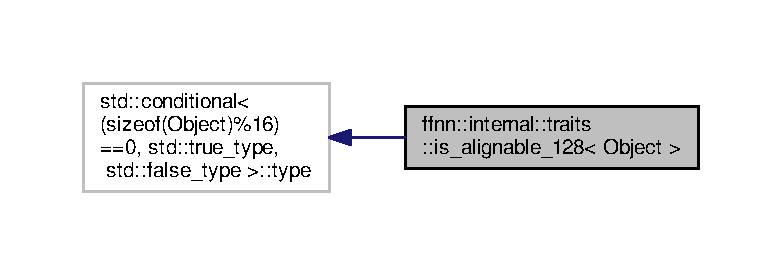
\includegraphics[width=350pt]{structffnn_1_1internal_1_1traits_1_1is__alignable__128__inherit__graph}
\end{center}
\end{figure}


Collaboration diagram for ffnn\-:\-:internal\-:\-:traits\-:\-:is\-\_\-alignable\-\_\-128$<$ Object $>$\-:\nopagebreak
\begin{figure}[H]
\begin{center}
\leavevmode
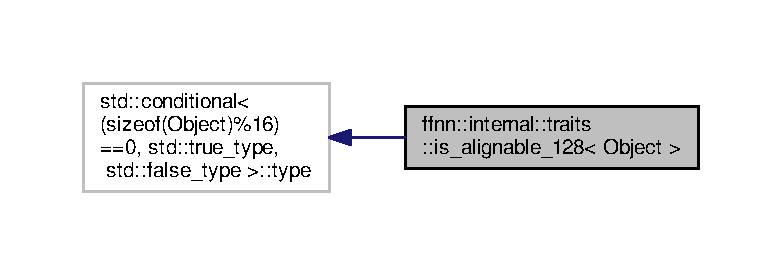
\includegraphics[width=350pt]{structffnn_1_1internal_1_1traits_1_1is__alignable__128__coll__graph}
\end{center}
\end{figure}


\subsection{Detailed Description}
\subsubsection*{template$<$class Object$>$struct ffnn\-::internal\-::traits\-::is\-\_\-alignable\-\_\-128$<$ Object $>$}

Has {\ttfamily value\-\_\-type == std\-::true\-\_\-type} if {\ttfamily Object} is a 16-\/byte alignable type. 

Has {\ttfamily value\-\_\-type == std\-::false\-\_\-type} otherwise 
\begin{DoxyParams}{Parameters}
{\em Object} & object to check \\
\hline
\end{DoxyParams}


The documentation for this struct was generated from the following file\-:\begin{DoxyCompactItemize}
\item 
/home/briancairl/packages/src/ffnn-\/cpp/ffnn/include/ffnn/internal/\hyperlink{traits_8h}{traits.\-h}\end{DoxyCompactItemize}

\hypertarget{structffnn_1_1neuron_1_1is__neuron}{\section{ffnn\-:\-:neuron\-:\-:is\-\_\-neuron$<$ Neuron\-Type $>$ Struct Template Reference}
\label{structffnn_1_1neuron_1_1is__neuron}\index{ffnn\-::neuron\-::is\-\_\-neuron$<$ Neuron\-Type $>$@{ffnn\-::neuron\-::is\-\_\-neuron$<$ Neuron\-Type $>$}}
}


{\ttfamily \#include \char`\"{}neuron.\-h\char`\"{}}

\subsection*{Static Public Attributes}
\begin{DoxyCompactItemize}
\item 
static constexpr bool \hyperlink{structffnn_1_1neuron_1_1is__neuron_adfafc315a5352f2a186959d8402490d1}{value} = Neuron\-Type\-::\-Is\-Neuron\-::value
\end{DoxyCompactItemize}


\subsection{Member Data Documentation}
\hypertarget{structffnn_1_1neuron_1_1is__neuron_adfafc315a5352f2a186959d8402490d1}{\index{ffnn\-::neuron\-::is\-\_\-neuron@{ffnn\-::neuron\-::is\-\_\-neuron}!value@{value}}
\index{value@{value}!ffnn::neuron::is_neuron@{ffnn\-::neuron\-::is\-\_\-neuron}}
\subsubsection[{value}]{\setlength{\rightskip}{0pt plus 5cm}template$<$typename Neuron\-Type $>$ constexpr bool {\bf ffnn\-::neuron\-::is\-\_\-neuron}$<$ Neuron\-Type $>$\-::value = Neuron\-Type\-::\-Is\-Neuron\-::value\hspace{0.3cm}{\ttfamily [static]}}}\label{structffnn_1_1neuron_1_1is__neuron_adfafc315a5352f2a186959d8402490d1}


The documentation for this struct was generated from the following file\-:\begin{DoxyCompactItemize}
\item 
/home/briancairl/packages/src/ffnn-\/cpp/ffnn/include/ffnn/neuron/\hyperlink{neuron_8h}{neuron.\-h}\end{DoxyCompactItemize}

\hypertarget{classffnn_1_1layer_1_1_layer}{\section{ffnn\-:\-:layer\-:\-:Layer$<$ Value\-Type, Enable\-Alignment $>$ Class Template Reference}
\label{classffnn_1_1layer_1_1_layer}\index{ffnn\-::layer\-::\-Layer$<$ Value\-Type, Enable\-Alignment $>$@{ffnn\-::layer\-::\-Layer$<$ Value\-Type, Enable\-Alignment $>$}}
}


Base object for all layer types.  




{\ttfamily \#include \char`\"{}layer.\-h\char`\"{}}



Inheritance diagram for ffnn\-:\-:layer\-:\-:Layer$<$ Value\-Type, Enable\-Alignment $>$\-:
\nopagebreak
\begin{figure}[H]
\begin{center}
\leavevmode
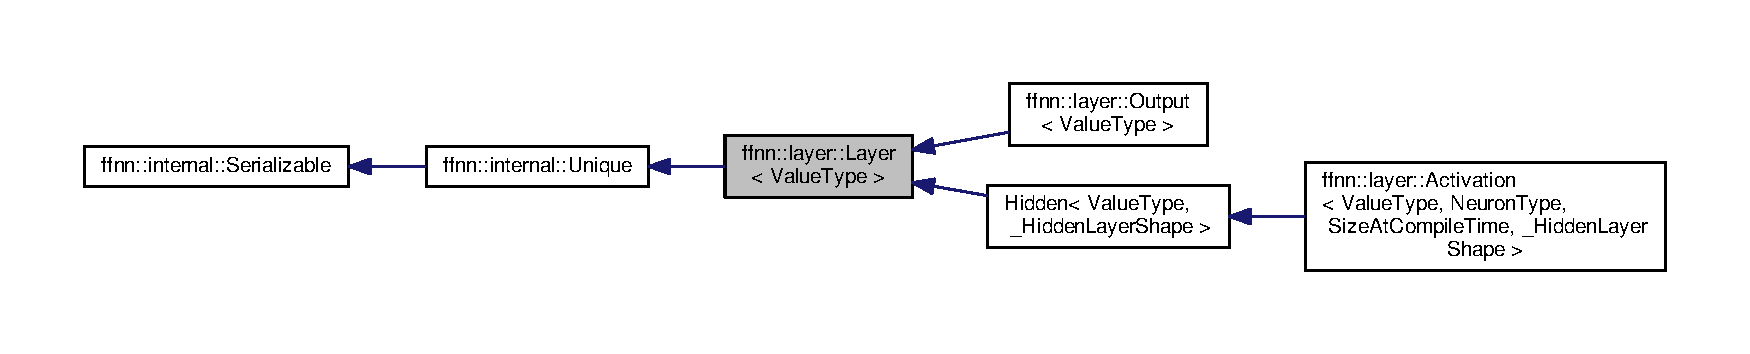
\includegraphics[width=240pt]{classffnn_1_1layer_1_1_layer__inherit__graph}
\end{center}
\end{figure}


Collaboration diagram for ffnn\-:\-:layer\-:\-:Layer$<$ Value\-Type, Enable\-Alignment $>$\-:
\nopagebreak
\begin{figure}[H]
\begin{center}
\leavevmode
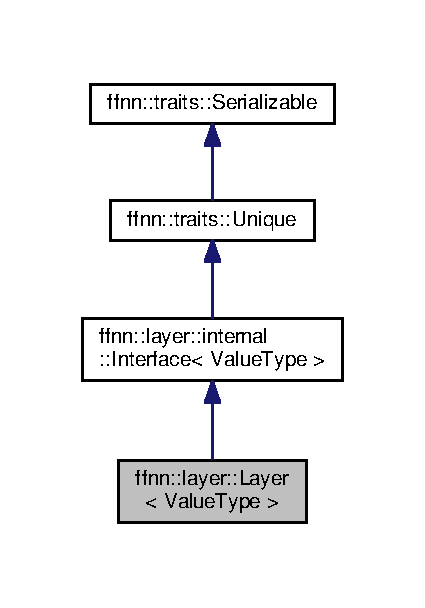
\includegraphics[width=240pt]{classffnn_1_1layer_1_1_layer__coll__graph}
\end{center}
\end{figure}
\subsection*{Public Types}
\begin{DoxyCompactItemize}
\item 
using \hyperlink{classffnn_1_1layer_1_1_layer_aef88481ace189a82a4576931ef964f7d}{Base} = \hyperlink{classffnn_1_1layer_1_1internal_1_1_interface}{internal\-::\-Interface}$<$ Value\-Type $>$
\begin{DoxyCompactList}\small\item\em Base type alias. \end{DoxyCompactList}\item 
using \hyperlink{classffnn_1_1layer_1_1_layer_af2600ebac2bf33f5a1fb3307d7ef1dbc}{Self} = \hyperlink{classffnn_1_1layer_1_1_layer}{Layer}$<$ Value\-Type, Enable\-Alignment $>$
\begin{DoxyCompactList}\small\item\em Self type alias. \end{DoxyCompactList}\item 
typedef boost\-::shared\-\_\-ptr$<$ \hyperlink{classffnn_1_1layer_1_1_layer_af2600ebac2bf33f5a1fb3307d7ef1dbc}{Self} $>$ \hyperlink{classffnn_1_1layer_1_1_layer_a0efb2ac9125e1fa8f905bd4eed765201}{Ptr}
\begin{DoxyCompactList}\small\item\em Shared resource standardization. \end{DoxyCompactList}\item 
typedef boost\-::shared\-\_\-ptr\\*
$<$ const \hyperlink{classffnn_1_1layer_1_1_layer_af2600ebac2bf33f5a1fb3307d7ef1dbc}{Self} $>$ \hyperlink{classffnn_1_1layer_1_1_layer_a6a0d0adbe331d1682e79d0c734fd3c72}{Const\-Ptr}
\begin{DoxyCompactList}\small\item\em Constant shared resource standardization. \end{DoxyCompactList}\item 
typedef std\-::conditional\\*
$<$ Enable\-Alignment\-::value, \\*
std\-::vector$<$ Value\-Type, \\*
Eigen\-::aligned\-\_\-allocator\\*
$<$ Value\-Type $>$ $>$, std\-::vector\\*
$<$ Value\-Type $>$ $>$\-::type \hyperlink{classffnn_1_1layer_1_1_layer_a981f9bea21513a7b61222b1cda9294e7}{Buffer\-Type}
\begin{DoxyCompactList}\small\item\em Buffer type standardization. \end{DoxyCompactList}\item 
typedef \hyperlink{classffnn_1_1layer_1_1internal_1_1_interface_a7f834e3365e5199bcbcd16d9abd63941}{Base\-::\-Scalar\-Type} \hyperlink{classffnn_1_1layer_1_1_layer_acec0144b094cc88faf0771b7ca8ce54c}{Scalar\-Type}
\begin{DoxyCompactList}\small\item\em Scalar type standardization. \end{DoxyCompactList}\item 
typedef \hyperlink{classffnn_1_1layer_1_1internal_1_1_interface_af0567642f60c65b5e87067226a54174b}{Base\-::\-Size\-Type} \hyperlink{classffnn_1_1layer_1_1_layer_a109e7a20f18d04e6d6f029c816b0958a}{Size\-Type}
\begin{DoxyCompactList}\small\item\em Size type standardization. \end{DoxyCompactList}\item 
typedef \hyperlink{classffnn_1_1layer_1_1internal_1_1_interface_adc5bb454329ebd51ac26579a43c006fd}{Base\-::\-Offset\-Type} \hyperlink{classffnn_1_1layer_1_1_layer_a5ed88ceefa1814e88fbccfdded6c9999}{Offset\-Type}
\begin{DoxyCompactList}\small\item\em Offset type standardization. \end{DoxyCompactList}\item 
typedef \hyperlink{classffnn_1_1layer_1_1internal_1_1_interface_a945709b1d0ea54a51539b80d04485f5f}{Base\-::\-Shape\-Type} \hyperlink{classffnn_1_1layer_1_1_layer_a83bc836aeacb312f6507ce1b47f8f7eb}{Shape\-Type}
\begin{DoxyCompactList}\small\item\em Dimension type standardization. \end{DoxyCompactList}\end{DoxyCompactItemize}
\subsection*{Public Member Functions}
\begin{DoxyCompactItemize}
\item 
\hyperlink{classffnn_1_1layer_1_1_layer_a7f4c075aeb084e8479c9a188181d51e8}{Layer} (const \hyperlink{classffnn_1_1layer_1_1internal_1_1_interface_a945709b1d0ea54a51539b80d04485f5f}{Shape\-Type} \&input\-\_\-shape, const \hyperlink{classffnn_1_1layer_1_1internal_1_1_interface_a945709b1d0ea54a51539b80d04485f5f}{Shape\-Type} \&output\-\_\-shape)
\begin{DoxyCompactList}\small\item\em Setup constructor. \end{DoxyCompactList}\item 
virtual \hyperlink{classffnn_1_1layer_1_1_layer_a9bcc2f1e58199ee9ba7ae279d12fc177}{$\sim$\-Layer} ()
\item 
virtual bool \hyperlink{classffnn_1_1layer_1_1_layer_af4d17333f47c016a379748b9318c7b50}{initialize} ()
\begin{DoxyCompactList}\small\item\em Initialize the layer. \end{DoxyCompactList}\item 
virtual bool \hyperlink{classffnn_1_1layer_1_1_layer_a5e7b9e250678604ce373ab2b82cdb8e1}{forward} ()
\begin{DoxyCompactList}\small\item\em Forward value propagation. \end{DoxyCompactList}\item 
virtual bool \hyperlink{classffnn_1_1layer_1_1_layer_ad5dc8961ffb0446f31952adc1da62746}{backward} ()
\begin{DoxyCompactList}\small\item\em Backward value propagation. \end{DoxyCompactList}\item 
virtual bool \hyperlink{classffnn_1_1layer_1_1_layer_a0e87cf29789204037c4678ee4bfc8756}{update} ()
\begin{DoxyCompactList}\small\item\em Applies layer weight updates. \end{DoxyCompactList}\item 
const \hyperlink{classffnn_1_1layer_1_1_layer_a981f9bea21513a7b61222b1cda9294e7}{Buffer\-Type} \& \hyperlink{classffnn_1_1layer_1_1_layer_a6c330b4b356e0ed768248943e763b87f}{get\-Input\-Buffer} () const 
\begin{DoxyCompactList}\small\item\em Exposes const reference to raw data input buffer. \end{DoxyCompactList}\item 
const \hyperlink{classffnn_1_1layer_1_1_layer_a981f9bea21513a7b61222b1cda9294e7}{Buffer\-Type} \& \hyperlink{classffnn_1_1layer_1_1_layer_a3f3adf7407280fcc52b529a01b265020}{get\-Backward\-Error\-Buffer} () const 
\begin{DoxyCompactList}\small\item\em Exposes const reference to raw data backward-\/error buffer. \end{DoxyCompactList}\item 
virtual \hyperlink{classffnn_1_1layer_1_1internal_1_1_interface_adc5bb454329ebd51ac26579a43c006fd}{Offset\-Type} \hyperlink{classffnn_1_1layer_1_1_layer_a6e3b760b6e6fa491b78f4ed0551fda85}{connect\-To\-Forward\-Layer} (const \hyperlink{classffnn_1_1layer_1_1_layer_af2600ebac2bf33f5a1fb3307d7ef1dbc}{Self} \&next, \hyperlink{classffnn_1_1layer_1_1internal_1_1_interface_adc5bb454329ebd51ac26579a43c006fd}{Offset\-Type} offset)=0
\begin{DoxyCompactList}\small\item\em Maps outputs of this layer to inputs of the next. \end{DoxyCompactList}\end{DoxyCompactItemize}
\subsection*{Protected Member Functions}
\begin{DoxyCompactItemize}
\item 
void \hyperlink{classffnn_1_1layer_1_1_layer_a5091f6ccef4d80254dd8caf72d13d136}{save} (\hyperlink{classffnn_1_1traits_1_1_serializable_a08d986df75d363fa79506d4f6045cb9f}{Output\-Archive} \&ar, \hyperlink{classffnn_1_1traits_1_1_serializable_a08924b3b7d20cb3cb6eafe517d4f7b30}{Version\-Type} version) const 
\begin{DoxyCompactList}\small\item\em Save serializer. \end{DoxyCompactList}\item 
void \hyperlink{classffnn_1_1layer_1_1_layer_a66c56645e54f6e864fb716fdc8858828}{load} (\hyperlink{classffnn_1_1traits_1_1_serializable_a6e626759259f8f370dd4303b4441a234}{Input\-Archive} \&ar, \hyperlink{classffnn_1_1traits_1_1_serializable_a08924b3b7d20cb3cb6eafe517d4f7b30}{Version\-Type} version)
\begin{DoxyCompactList}\small\item\em Load serializer. \end{DoxyCompactList}\item 
\hyperlink{classffnn_1_1layer_1_1internal_1_1_interface_af0567642f60c65b5e87067226a54174b}{Size\-Type} \hyperlink{classffnn_1_1layer_1_1_layer_ad1ca9fa504ca3fc9847d5489dc392ea8}{evaluate\-Input\-Size} () const 
\begin{DoxyCompactList}\small\item\em Counts the number of inputs from outputs of previous layers. \end{DoxyCompactList}\item 
\hyperlink{classffnn_1_1layer_1_1internal_1_1_interface_adc5bb454329ebd51ac26579a43c006fd}{Offset\-Type} \hyperlink{classffnn_1_1layer_1_1_layer_a303d4fc17e59e1cc3081e5a28d6d9417}{connect\-Input\-Layers} ()
\begin{DoxyCompactList}\small\item\em Connects all previous layer to \hyperlink{classffnn_1_1layer_1_1_layer}{Layer} input. \end{DoxyCompactList}\end{DoxyCompactItemize}
\subsection*{Protected Attributes}
\begin{DoxyCompactItemize}
\item 
std\-::map$<$ std\-::string, \\*
typename \hyperlink{classffnn_1_1layer_1_1_layer_a0efb2ac9125e1fa8f905bd4eed765201}{Self\-::\-Ptr} $>$ \hyperlink{classffnn_1_1layer_1_1_layer_ad665f209da80c13770f2b6a790d3ed4f}{prev\-\_\-}
\begin{DoxyCompactList}\small\item\em Pointers to previous layers. \end{DoxyCompactList}\item 
\hyperlink{classffnn_1_1layer_1_1_layer_a981f9bea21513a7b61222b1cda9294e7}{Buffer\-Type} \hyperlink{classffnn_1_1layer_1_1_layer_a8595d0898a1530aaec71aec487037655}{input\-\_\-buffer\-\_\-}
\begin{DoxyCompactList}\small\item\em Raw input value buffer. \end{DoxyCompactList}\item 
\hyperlink{classffnn_1_1layer_1_1_layer_a981f9bea21513a7b61222b1cda9294e7}{Buffer\-Type} \hyperlink{classffnn_1_1layer_1_1_layer_a1be25b9933d64c2964b4260db770ad48}{backward\-\_\-error\-\_\-buffer\-\_\-}
\begin{DoxyCompactList}\small\item\em Raw bakward error value buffer. \end{DoxyCompactList}\end{DoxyCompactItemize}
\subsection*{Friends}
\begin{DoxyCompactItemize}
\item 
{\footnotesize template$<$typename Layer\-Type $>$ }\\bool \hyperlink{classffnn_1_1layer_1_1_layer_afbf91ff52dc8c3e894968dcc27cdecd5}{connect} (const typename Layer\-Type\-::\-Ptr \&from, const typename Layer\-Type\-::\-Ptr \&to)
\begin{DoxyCompactList}\small\item\em Connects \hyperlink{classffnn_1_1layer_1_1_layer}{Layer} objects. \end{DoxyCompactList}\end{DoxyCompactItemize}


\subsection{Detailed Description}
\subsubsection*{template$<$typename Value\-Type, class Enable\-Alignment = std\-::true\-\_\-type$>$class ffnn\-::layer\-::\-Layer$<$ Value\-Type, Enable\-Alignment $>$}

Base object for all layer types. 

\subsection{Member Typedef Documentation}
\hypertarget{classffnn_1_1layer_1_1_layer_aef88481ace189a82a4576931ef964f7d}{\index{ffnn\-::layer\-::\-Layer@{ffnn\-::layer\-::\-Layer}!Base@{Base}}
\index{Base@{Base}!ffnn::layer::Layer@{ffnn\-::layer\-::\-Layer}}
\subsubsection[{Base}]{\setlength{\rightskip}{0pt plus 5cm}template$<$typename Value\-Type, class Enable\-Alignment = std\-::true\-\_\-type$>$ using {\bf ffnn\-::layer\-::\-Layer}$<$ Value\-Type, Enable\-Alignment $>$\-::{\bf Base} =  {\bf internal\-::\-Interface}$<$Value\-Type$>$}}\label{classffnn_1_1layer_1_1_layer_aef88481ace189a82a4576931ef964f7d}


Base type alias. 

\hypertarget{classffnn_1_1layer_1_1_layer_a981f9bea21513a7b61222b1cda9294e7}{\index{ffnn\-::layer\-::\-Layer@{ffnn\-::layer\-::\-Layer}!Buffer\-Type@{Buffer\-Type}}
\index{Buffer\-Type@{Buffer\-Type}!ffnn::layer::Layer@{ffnn\-::layer\-::\-Layer}}
\subsubsection[{Buffer\-Type}]{\setlength{\rightskip}{0pt plus 5cm}template$<$typename Value\-Type, class Enable\-Alignment = std\-::true\-\_\-type$>$ typedef std\-::conditional$<$ Enable\-Alignment\-::value, std\-::vector$<$Value\-Type, Eigen\-::aligned\-\_\-allocator$<$Value\-Type$>$ $>$, std\-::vector$<$Value\-Type$>$ $>$\-::type {\bf ffnn\-::layer\-::\-Layer}$<$ Value\-Type, Enable\-Alignment $>$\-::{\bf Buffer\-Type}}}\label{classffnn_1_1layer_1_1_layer_a981f9bea21513a7b61222b1cda9294e7}


Buffer type standardization. 

\hypertarget{classffnn_1_1layer_1_1_layer_a6a0d0adbe331d1682e79d0c734fd3c72}{\index{ffnn\-::layer\-::\-Layer@{ffnn\-::layer\-::\-Layer}!Const\-Ptr@{Const\-Ptr}}
\index{Const\-Ptr@{Const\-Ptr}!ffnn::layer::Layer@{ffnn\-::layer\-::\-Layer}}
\subsubsection[{Const\-Ptr}]{\setlength{\rightskip}{0pt plus 5cm}template$<$typename Value\-Type, class Enable\-Alignment = std\-::true\-\_\-type$>$ typedef boost\-::shared\-\_\-ptr$<$const {\bf Self}$>$ {\bf ffnn\-::layer\-::\-Layer}$<$ Value\-Type, Enable\-Alignment $>$\-::{\bf Const\-Ptr}}}\label{classffnn_1_1layer_1_1_layer_a6a0d0adbe331d1682e79d0c734fd3c72}


Constant shared resource standardization. 

\hypertarget{classffnn_1_1layer_1_1_layer_a5ed88ceefa1814e88fbccfdded6c9999}{\index{ffnn\-::layer\-::\-Layer@{ffnn\-::layer\-::\-Layer}!Offset\-Type@{Offset\-Type}}
\index{Offset\-Type@{Offset\-Type}!ffnn::layer::Layer@{ffnn\-::layer\-::\-Layer}}
\subsubsection[{Offset\-Type}]{\setlength{\rightskip}{0pt plus 5cm}template$<$typename Value\-Type, class Enable\-Alignment = std\-::true\-\_\-type$>$ typedef {\bf Base\-::\-Offset\-Type} {\bf ffnn\-::layer\-::\-Layer}$<$ Value\-Type, Enable\-Alignment $>$\-::{\bf Offset\-Type}}}\label{classffnn_1_1layer_1_1_layer_a5ed88ceefa1814e88fbccfdded6c9999}


Offset type standardization. 

\hypertarget{classffnn_1_1layer_1_1_layer_a0efb2ac9125e1fa8f905bd4eed765201}{\index{ffnn\-::layer\-::\-Layer@{ffnn\-::layer\-::\-Layer}!Ptr@{Ptr}}
\index{Ptr@{Ptr}!ffnn::layer::Layer@{ffnn\-::layer\-::\-Layer}}
\subsubsection[{Ptr}]{\setlength{\rightskip}{0pt plus 5cm}template$<$typename Value\-Type, class Enable\-Alignment = std\-::true\-\_\-type$>$ typedef boost\-::shared\-\_\-ptr$<${\bf Self}$>$ {\bf ffnn\-::layer\-::\-Layer}$<$ Value\-Type, Enable\-Alignment $>$\-::{\bf Ptr}}}\label{classffnn_1_1layer_1_1_layer_a0efb2ac9125e1fa8f905bd4eed765201}


Shared resource standardization. 

\hypertarget{classffnn_1_1layer_1_1_layer_acec0144b094cc88faf0771b7ca8ce54c}{\index{ffnn\-::layer\-::\-Layer@{ffnn\-::layer\-::\-Layer}!Scalar\-Type@{Scalar\-Type}}
\index{Scalar\-Type@{Scalar\-Type}!ffnn::layer::Layer@{ffnn\-::layer\-::\-Layer}}
\subsubsection[{Scalar\-Type}]{\setlength{\rightskip}{0pt plus 5cm}template$<$typename Value\-Type, class Enable\-Alignment = std\-::true\-\_\-type$>$ typedef {\bf Base\-::\-Scalar\-Type} {\bf ffnn\-::layer\-::\-Layer}$<$ Value\-Type, Enable\-Alignment $>$\-::{\bf Scalar\-Type}}}\label{classffnn_1_1layer_1_1_layer_acec0144b094cc88faf0771b7ca8ce54c}


Scalar type standardization. 

\hypertarget{classffnn_1_1layer_1_1_layer_af2600ebac2bf33f5a1fb3307d7ef1dbc}{\index{ffnn\-::layer\-::\-Layer@{ffnn\-::layer\-::\-Layer}!Self@{Self}}
\index{Self@{Self}!ffnn::layer::Layer@{ffnn\-::layer\-::\-Layer}}
\subsubsection[{Self}]{\setlength{\rightskip}{0pt plus 5cm}template$<$typename Value\-Type, class Enable\-Alignment = std\-::true\-\_\-type$>$ using {\bf ffnn\-::layer\-::\-Layer}$<$ Value\-Type, Enable\-Alignment $>$\-::{\bf Self} =  {\bf Layer}$<$Value\-Type, Enable\-Alignment$>$}}\label{classffnn_1_1layer_1_1_layer_af2600ebac2bf33f5a1fb3307d7ef1dbc}


Self type alias. 

\hypertarget{classffnn_1_1layer_1_1_layer_a83bc836aeacb312f6507ce1b47f8f7eb}{\index{ffnn\-::layer\-::\-Layer@{ffnn\-::layer\-::\-Layer}!Shape\-Type@{Shape\-Type}}
\index{Shape\-Type@{Shape\-Type}!ffnn::layer::Layer@{ffnn\-::layer\-::\-Layer}}
\subsubsection[{Shape\-Type}]{\setlength{\rightskip}{0pt plus 5cm}template$<$typename Value\-Type, class Enable\-Alignment = std\-::true\-\_\-type$>$ typedef {\bf Base\-::\-Shape\-Type} {\bf ffnn\-::layer\-::\-Layer}$<$ Value\-Type, Enable\-Alignment $>$\-::{\bf Shape\-Type}}}\label{classffnn_1_1layer_1_1_layer_a83bc836aeacb312f6507ce1b47f8f7eb}


Dimension type standardization. 

\hypertarget{classffnn_1_1layer_1_1_layer_a109e7a20f18d04e6d6f029c816b0958a}{\index{ffnn\-::layer\-::\-Layer@{ffnn\-::layer\-::\-Layer}!Size\-Type@{Size\-Type}}
\index{Size\-Type@{Size\-Type}!ffnn::layer::Layer@{ffnn\-::layer\-::\-Layer}}
\subsubsection[{Size\-Type}]{\setlength{\rightskip}{0pt plus 5cm}template$<$typename Value\-Type, class Enable\-Alignment = std\-::true\-\_\-type$>$ typedef {\bf Base\-::\-Size\-Type} {\bf ffnn\-::layer\-::\-Layer}$<$ Value\-Type, Enable\-Alignment $>$\-::{\bf Size\-Type}}}\label{classffnn_1_1layer_1_1_layer_a109e7a20f18d04e6d6f029c816b0958a}


Size type standardization. 



\subsection{Constructor \& Destructor Documentation}
\hypertarget{classffnn_1_1layer_1_1_layer_a7f4c075aeb084e8479c9a188181d51e8}{\index{ffnn\-::layer\-::\-Layer@{ffnn\-::layer\-::\-Layer}!Layer@{Layer}}
\index{Layer@{Layer}!ffnn::layer::Layer@{ffnn\-::layer\-::\-Layer}}
\subsubsection[{Layer}]{\setlength{\rightskip}{0pt plus 5cm}template$<$typename Value\-Type , class Enable\-Alignment $>$ {\bf ffnn\-::layer\-::\-Layer}$<$ Value\-Type, Enable\-Alignment $>$\-::{\bf Layer} (
\begin{DoxyParamCaption}
\item[{const {\bf Shape\-Type} \&}]{input\-\_\-shape, }
\item[{const {\bf Shape\-Type} \&}]{output\-\_\-shape}
\end{DoxyParamCaption}
)}}\label{classffnn_1_1layer_1_1_layer_a7f4c075aeb084e8479c9a188181d51e8}


Setup constructor. 


\begin{DoxyParams}{Parameters}
{\em input\-\_\-shape} & number of inputs to the \hyperlink{classffnn_1_1layer_1_1_layer}{Layer} \\
\hline
{\em output\-\_\-shape} & number of outputs from the \hyperlink{classffnn_1_1layer_1_1_layer}{Layer} \\
\hline
\end{DoxyParams}
\hypertarget{classffnn_1_1layer_1_1_layer_a9bcc2f1e58199ee9ba7ae279d12fc177}{\index{ffnn\-::layer\-::\-Layer@{ffnn\-::layer\-::\-Layer}!$\sim$\-Layer@{$\sim$\-Layer}}
\index{$\sim$\-Layer@{$\sim$\-Layer}!ffnn::layer::Layer@{ffnn\-::layer\-::\-Layer}}
\subsubsection[{$\sim$\-Layer}]{\setlength{\rightskip}{0pt plus 5cm}template$<$typename Value\-Type , class Enable\-Alignment $>$ {\bf ffnn\-::layer\-::\-Layer}$<$ Value\-Type, Enable\-Alignment $>$\-::$\sim${\bf Layer} (
\begin{DoxyParamCaption}
{}
\end{DoxyParamCaption}
)\hspace{0.3cm}{\ttfamily [virtual]}}}\label{classffnn_1_1layer_1_1_layer_a9bcc2f1e58199ee9ba7ae279d12fc177}


\subsection{Member Function Documentation}
\hypertarget{classffnn_1_1layer_1_1_layer_ad5dc8961ffb0446f31952adc1da62746}{\index{ffnn\-::layer\-::\-Layer@{ffnn\-::layer\-::\-Layer}!backward@{backward}}
\index{backward@{backward}!ffnn::layer::Layer@{ffnn\-::layer\-::\-Layer}}
\subsubsection[{backward}]{\setlength{\rightskip}{0pt plus 5cm}template$<$typename Value\-Type, class Enable\-Alignment = std\-::true\-\_\-type$>$ virtual bool {\bf ffnn\-::layer\-::\-Layer}$<$ Value\-Type, Enable\-Alignment $>$\-::backward (
\begin{DoxyParamCaption}
{}
\end{DoxyParamCaption}
)\hspace{0.3cm}{\ttfamily [inline]}, {\ttfamily [virtual]}}}\label{classffnn_1_1layer_1_1_layer_ad5dc8961ffb0446f31952adc1da62746}


Backward value propagation. 


\begin{DoxyRetVals}{Return values}
{\em true} & if backward-\/propagation succeeded \\
\hline
{\em false} & otherwise \\
\hline
\end{DoxyRetVals}


Reimplemented in \hyperlink{classffnn_1_1layer_1_1_convolution_af079973fdb795f4ccd902a00c4d96d3b}{ffnn\-::layer\-::\-Convolution$<$ Value\-Type, Height\-At\-Compile\-Time, Width\-At\-Compile\-Time, Depth\-At\-Compile\-Time, Filter\-Height\-At\-Compile\-Time, Filter\-Width\-At\-Compile\-Time, Filter\-Count\-At\-Compile\-Time, Stride\-At\-Compile\-Time, Mode $>$}, \hyperlink{classffnn_1_1layer_1_1_sparsely_connected_a597ea83c83e8f4f64a1fb7f17a1ea015}{ffnn\-::layer\-::\-Sparsely\-Connected$<$ Value\-Type, Inputs\-At\-Compile\-Time, Outputs\-At\-Compile\-Time $>$}, \hyperlink{classffnn_1_1layer_1_1_fully_connected_afd5c1a006cf33a47cb7e2a982fe4cd6d}{ffnn\-::layer\-::\-Fully\-Connected$<$ Value\-Type, Inputs\-At\-Compile\-Time, Outputs\-At\-Compile\-Time $>$}, \hyperlink{classffnn_1_1layer_1_1_hidden_a246152dfed00bbacb94fbbd6712acea0}{ffnn\-::layer\-::\-Hidden$<$ Value\-Type, Input\-Height\-At\-Compile\-Time, Input\-Width\-At\-Compile\-Time, Output\-Height\-At\-Compile\-Time, Output\-Width\-At\-Compile\-Time, \-\_\-\-Input\-Block\-Type, \-\_\-\-Output\-Block\-Type, \-\_\-\-Input\-Mapping\-Type, \-\_\-\-Output\-Mapping\-Type $>$}, \hyperlink{classffnn_1_1layer_1_1_hidden_a246152dfed00bbacb94fbbd6712acea0}{ffnn\-::layer\-::\-Hidden$<$ Value\-Type, Inputs\-At\-Compile\-Time, 1, Outputs\-At\-Compile\-Time, 1 $>$}, \hyperlink{classffnn_1_1layer_1_1_hidden_a246152dfed00bbacb94fbbd6712acea0}{ffnn\-::layer\-::\-Hidden$<$ Value\-Type, Size\-At\-Compile\-Time, 1, Size\-At\-Compile\-Time, 1 $>$}, \hyperlink{classffnn_1_1layer_1_1_hidden_a246152dfed00bbacb94fbbd6712acea0}{ffnn\-::layer\-::\-Hidden$<$ Value\-Type, embed\-\_\-dimension$<$ Mode, Col\-Embedding $>$(\-Height\-At\-Compile\-Time, Depth\-At\-Compile\-Time), embed\-\_\-dimension$<$ Mode, Row\-Embedding $>$(\-Width\-At\-Compile\-Time, Depth\-At\-Compile\-Time), embed\-\_\-dimension$<$ Mode, Col\-Embedding $>$(output\-\_\-dimension(\-Height\-At\-Compile\-Time, Filter\-Height\-At\-Compile\-Time, Stride\-At\-Compile\-Time), Filter\-Count\-At\-Compile\-Time), embed\-\_\-dimension$<$ Mode, Row\-Embedding $>$(output\-\_\-dimension(\-Width\-At\-Compile\-Time, Filter\-Width\-At\-Compile\-Time, Stride\-At\-Compile\-Time), Filter\-Count\-At\-Compile\-Time)$>$}, and \hyperlink{classffnn_1_1layer_1_1_activation_a3c4284245343f2132dd28eaf7ffbed47}{ffnn\-::layer\-::\-Activation$<$ Value\-Type, Neuron\-Type, Size\-At\-Compile\-Time $>$}.

\hypertarget{classffnn_1_1layer_1_1_layer_a303d4fc17e59e1cc3081e5a28d6d9417}{\index{ffnn\-::layer\-::\-Layer@{ffnn\-::layer\-::\-Layer}!connect\-Input\-Layers@{connect\-Input\-Layers}}
\index{connect\-Input\-Layers@{connect\-Input\-Layers}!ffnn::layer::Layer@{ffnn\-::layer\-::\-Layer}}
\subsubsection[{connect\-Input\-Layers}]{\setlength{\rightskip}{0pt plus 5cm}template$<$typename Value\-Type , class Enable\-Alignment $>$ {\bf Layer}$<$ Value\-Type, Enable\-Alignment $>$\-::{\bf Offset\-Type} {\bf ffnn\-::layer\-::\-Layer}$<$ Value\-Type, Enable\-Alignment $>$\-::connect\-Input\-Layers (
\begin{DoxyParamCaption}
{}
\end{DoxyParamCaption}
)\hspace{0.3cm}{\ttfamily [protected]}}}\label{classffnn_1_1layer_1_1_layer_a303d4fc17e59e1cc3081e5a28d6d9417}


Connects all previous layer to \hyperlink{classffnn_1_1layer_1_1_layer}{Layer} input. 


\begin{DoxyRetVals}{Return values}
{\em $<$code$>$input\-\_\-shape\-\_\-.\-size()$<$/code$>$} & \\
\hline
\end{DoxyRetVals}
\hypertarget{classffnn_1_1layer_1_1_layer_a6e3b760b6e6fa491b78f4ed0551fda85}{\index{ffnn\-::layer\-::\-Layer@{ffnn\-::layer\-::\-Layer}!connect\-To\-Forward\-Layer@{connect\-To\-Forward\-Layer}}
\index{connect\-To\-Forward\-Layer@{connect\-To\-Forward\-Layer}!ffnn::layer::Layer@{ffnn\-::layer\-::\-Layer}}
\subsubsection[{connect\-To\-Forward\-Layer}]{\setlength{\rightskip}{0pt plus 5cm}template$<$typename Value\-Type, class Enable\-Alignment = std\-::true\-\_\-type$>$ virtual {\bf Offset\-Type} {\bf ffnn\-::layer\-::\-Layer}$<$ Value\-Type, Enable\-Alignment $>$\-::connect\-To\-Forward\-Layer (
\begin{DoxyParamCaption}
\item[{const {\bf Self} \&}]{next, }
\item[{{\bf Offset\-Type}}]{offset}
\end{DoxyParamCaption}
)\hspace{0.3cm}{\ttfamily [pure virtual]}}}\label{classffnn_1_1layer_1_1_layer_a6e3b760b6e6fa491b78f4ed0551fda85}


Maps outputs of this layer to inputs of the next. 


\begin{DoxyParams}{Parameters}
{\em next} & a subsequent layer \\
\hline
{\em offset} & offset index of a memory location in the input buffer of the next layer \\
\hline
\end{DoxyParams}

\begin{DoxyRetVals}{Return values}
{\em $<$code$>$offset} & + output\-\_\-shape\-\_\-.\-size() \\
\hline
\end{DoxyRetVals}
\hypertarget{classffnn_1_1layer_1_1_layer_ad1ca9fa504ca3fc9847d5489dc392ea8}{\index{ffnn\-::layer\-::\-Layer@{ffnn\-::layer\-::\-Layer}!evaluate\-Input\-Size@{evaluate\-Input\-Size}}
\index{evaluate\-Input\-Size@{evaluate\-Input\-Size}!ffnn::layer::Layer@{ffnn\-::layer\-::\-Layer}}
\subsubsection[{evaluate\-Input\-Size}]{\setlength{\rightskip}{0pt plus 5cm}template$<$typename Value\-Type , class Enable\-Alignment $>$ {\bf Layer}$<$ Value\-Type, Enable\-Alignment $>$\-::{\bf Size\-Type} {\bf ffnn\-::layer\-::\-Layer}$<$ Value\-Type, Enable\-Alignment $>$\-::evaluate\-Input\-Size (
\begin{DoxyParamCaption}
{}
\end{DoxyParamCaption}
) const\hspace{0.3cm}{\ttfamily [protected]}, {\ttfamily [virtual]}}}\label{classffnn_1_1layer_1_1_layer_ad1ca9fa504ca3fc9847d5489dc392ea8}


Counts the number of inputs from outputs of previous layers. 

\begin{DoxyReturn}{Returns}
total input count 
\end{DoxyReturn}


Reimplemented from \hyperlink{classffnn_1_1layer_1_1internal_1_1_interface_aae590ebe90408887805743c5e364dd45}{ffnn\-::layer\-::internal\-::\-Interface$<$ Value\-Type $>$}.

\hypertarget{classffnn_1_1layer_1_1_layer_a5e7b9e250678604ce373ab2b82cdb8e1}{\index{ffnn\-::layer\-::\-Layer@{ffnn\-::layer\-::\-Layer}!forward@{forward}}
\index{forward@{forward}!ffnn::layer::Layer@{ffnn\-::layer\-::\-Layer}}
\subsubsection[{forward}]{\setlength{\rightskip}{0pt plus 5cm}template$<$typename Value\-Type, class Enable\-Alignment = std\-::true\-\_\-type$>$ virtual bool {\bf ffnn\-::layer\-::\-Layer}$<$ Value\-Type, Enable\-Alignment $>$\-::forward (
\begin{DoxyParamCaption}
{}
\end{DoxyParamCaption}
)\hspace{0.3cm}{\ttfamily [inline]}, {\ttfamily [virtual]}}}\label{classffnn_1_1layer_1_1_layer_a5e7b9e250678604ce373ab2b82cdb8e1}


Forward value propagation. 


\begin{DoxyRetVals}{Return values}
{\em true} & if forward-\/propagation succeeded \\
\hline
{\em false} & otherwise \\
\hline
\end{DoxyRetVals}


Reimplemented in \hyperlink{classffnn_1_1layer_1_1_convolution_a7da09bc158b4c6f61bc02ea3bc6f8cee}{ffnn\-::layer\-::\-Convolution$<$ Value\-Type, Height\-At\-Compile\-Time, Width\-At\-Compile\-Time, Depth\-At\-Compile\-Time, Filter\-Height\-At\-Compile\-Time, Filter\-Width\-At\-Compile\-Time, Filter\-Count\-At\-Compile\-Time, Stride\-At\-Compile\-Time, Mode $>$}, \hyperlink{classffnn_1_1layer_1_1_sparsely_connected_a53f1d9a2edfdd2e47164b24121c23acc}{ffnn\-::layer\-::\-Sparsely\-Connected$<$ Value\-Type, Inputs\-At\-Compile\-Time, Outputs\-At\-Compile\-Time $>$}, \hyperlink{classffnn_1_1layer_1_1_fully_connected_ac49087ab2d66019f2d0244c76987fa50}{ffnn\-::layer\-::\-Fully\-Connected$<$ Value\-Type, Inputs\-At\-Compile\-Time, Outputs\-At\-Compile\-Time $>$}, \hyperlink{classffnn_1_1layer_1_1_hidden_a41fdfb60b5340c0af46c7c731237e280}{ffnn\-::layer\-::\-Hidden$<$ Value\-Type, Input\-Height\-At\-Compile\-Time, Input\-Width\-At\-Compile\-Time, Output\-Height\-At\-Compile\-Time, Output\-Width\-At\-Compile\-Time, \-\_\-\-Input\-Block\-Type, \-\_\-\-Output\-Block\-Type, \-\_\-\-Input\-Mapping\-Type, \-\_\-\-Output\-Mapping\-Type $>$}, \hyperlink{classffnn_1_1layer_1_1_hidden_a41fdfb60b5340c0af46c7c731237e280}{ffnn\-::layer\-::\-Hidden$<$ Value\-Type, Inputs\-At\-Compile\-Time, 1, Outputs\-At\-Compile\-Time, 1 $>$}, \hyperlink{classffnn_1_1layer_1_1_hidden_a41fdfb60b5340c0af46c7c731237e280}{ffnn\-::layer\-::\-Hidden$<$ Value\-Type, Size\-At\-Compile\-Time, 1, Size\-At\-Compile\-Time, 1 $>$}, \hyperlink{classffnn_1_1layer_1_1_hidden_a41fdfb60b5340c0af46c7c731237e280}{ffnn\-::layer\-::\-Hidden$<$ Value\-Type, embed\-\_\-dimension$<$ Mode, Col\-Embedding $>$(\-Height\-At\-Compile\-Time, Depth\-At\-Compile\-Time), embed\-\_\-dimension$<$ Mode, Row\-Embedding $>$(\-Width\-At\-Compile\-Time, Depth\-At\-Compile\-Time), embed\-\_\-dimension$<$ Mode, Col\-Embedding $>$(output\-\_\-dimension(\-Height\-At\-Compile\-Time, Filter\-Height\-At\-Compile\-Time, Stride\-At\-Compile\-Time), Filter\-Count\-At\-Compile\-Time), embed\-\_\-dimension$<$ Mode, Row\-Embedding $>$(output\-\_\-dimension(\-Width\-At\-Compile\-Time, Filter\-Width\-At\-Compile\-Time, Stride\-At\-Compile\-Time), Filter\-Count\-At\-Compile\-Time)$>$}, and \hyperlink{classffnn_1_1layer_1_1_activation_aa7f88c8bc20589dc51d9dd615b8c4580}{ffnn\-::layer\-::\-Activation$<$ Value\-Type, Neuron\-Type, Size\-At\-Compile\-Time $>$}.

\hypertarget{classffnn_1_1layer_1_1_layer_a3f3adf7407280fcc52b529a01b265020}{\index{ffnn\-::layer\-::\-Layer@{ffnn\-::layer\-::\-Layer}!get\-Backward\-Error\-Buffer@{get\-Backward\-Error\-Buffer}}
\index{get\-Backward\-Error\-Buffer@{get\-Backward\-Error\-Buffer}!ffnn::layer::Layer@{ffnn\-::layer\-::\-Layer}}
\subsubsection[{get\-Backward\-Error\-Buffer}]{\setlength{\rightskip}{0pt plus 5cm}template$<$typename Value\-Type, class Enable\-Alignment = std\-::true\-\_\-type$>$ const {\bf Buffer\-Type}\& {\bf ffnn\-::layer\-::\-Layer}$<$ Value\-Type, Enable\-Alignment $>$\-::get\-Backward\-Error\-Buffer (
\begin{DoxyParamCaption}
{}
\end{DoxyParamCaption}
) const\hspace{0.3cm}{\ttfamily [inline]}}}\label{classffnn_1_1layer_1_1_layer_a3f3adf7407280fcc52b529a01b265020}


Exposes const reference to raw data backward-\/error buffer. 

\hypertarget{classffnn_1_1layer_1_1_layer_a6c330b4b356e0ed768248943e763b87f}{\index{ffnn\-::layer\-::\-Layer@{ffnn\-::layer\-::\-Layer}!get\-Input\-Buffer@{get\-Input\-Buffer}}
\index{get\-Input\-Buffer@{get\-Input\-Buffer}!ffnn::layer::Layer@{ffnn\-::layer\-::\-Layer}}
\subsubsection[{get\-Input\-Buffer}]{\setlength{\rightskip}{0pt plus 5cm}template$<$typename Value\-Type, class Enable\-Alignment = std\-::true\-\_\-type$>$ const {\bf Buffer\-Type}\& {\bf ffnn\-::layer\-::\-Layer}$<$ Value\-Type, Enable\-Alignment $>$\-::get\-Input\-Buffer (
\begin{DoxyParamCaption}
{}
\end{DoxyParamCaption}
) const\hspace{0.3cm}{\ttfamily [inline]}}}\label{classffnn_1_1layer_1_1_layer_a6c330b4b356e0ed768248943e763b87f}


Exposes const reference to raw data input buffer. 

\hypertarget{classffnn_1_1layer_1_1_layer_af4d17333f47c016a379748b9318c7b50}{\index{ffnn\-::layer\-::\-Layer@{ffnn\-::layer\-::\-Layer}!initialize@{initialize}}
\index{initialize@{initialize}!ffnn::layer::Layer@{ffnn\-::layer\-::\-Layer}}
\subsubsection[{initialize}]{\setlength{\rightskip}{0pt plus 5cm}template$<$typename Value\-Type , class Enable\-Alignment $>$ bool {\bf ffnn\-::layer\-::\-Layer}$<$ Value\-Type, Enable\-Alignment $>$\-::initialize (
\begin{DoxyParamCaption}
{}
\end{DoxyParamCaption}
)\hspace{0.3cm}{\ttfamily [virtual]}}}\label{classffnn_1_1layer_1_1_layer_af4d17333f47c016a379748b9318c7b50}


Initialize the layer. 



Implements \hyperlink{classffnn_1_1layer_1_1internal_1_1_interface_a4159d9d163a0bd5287cc02c91b5baba8}{ffnn\-::layer\-::internal\-::\-Interface$<$ Value\-Type $>$}.



Reimplemented in \hyperlink{classffnn_1_1layer_1_1_convolution_ad438bd0584804863bd064a493e2892a1}{ffnn\-::layer\-::\-Convolution$<$ Value\-Type, Height\-At\-Compile\-Time, Width\-At\-Compile\-Time, Depth\-At\-Compile\-Time, Filter\-Height\-At\-Compile\-Time, Filter\-Width\-At\-Compile\-Time, Filter\-Count\-At\-Compile\-Time, Stride\-At\-Compile\-Time, Mode $>$}, \hyperlink{classffnn_1_1layer_1_1_sparsely_connected_abb2966b5e7813c43ae2ea5448188a9fb}{ffnn\-::layer\-::\-Sparsely\-Connected$<$ Value\-Type, Inputs\-At\-Compile\-Time, Outputs\-At\-Compile\-Time $>$}, \hyperlink{classffnn_1_1layer_1_1_fully_connected_aec414194202f845b866b0e8b2a51235c}{ffnn\-::layer\-::\-Fully\-Connected$<$ Value\-Type, Inputs\-At\-Compile\-Time, Outputs\-At\-Compile\-Time $>$}, \hyperlink{classffnn_1_1layer_1_1_hidden_a3b5458a771fcf2371376049d85afbc92}{ffnn\-::layer\-::\-Hidden$<$ Value\-Type, Input\-Height\-At\-Compile\-Time, Input\-Width\-At\-Compile\-Time, Output\-Height\-At\-Compile\-Time, Output\-Width\-At\-Compile\-Time, \-\_\-\-Input\-Block\-Type, \-\_\-\-Output\-Block\-Type, \-\_\-\-Input\-Mapping\-Type, \-\_\-\-Output\-Mapping\-Type $>$}, \hyperlink{classffnn_1_1layer_1_1_hidden_a3b5458a771fcf2371376049d85afbc92}{ffnn\-::layer\-::\-Hidden$<$ Value\-Type, Inputs\-At\-Compile\-Time, 1, Outputs\-At\-Compile\-Time, 1 $>$}, \hyperlink{classffnn_1_1layer_1_1_hidden_a3b5458a771fcf2371376049d85afbc92}{ffnn\-::layer\-::\-Hidden$<$ Value\-Type, Size\-At\-Compile\-Time, 1, Size\-At\-Compile\-Time, 1 $>$}, \hyperlink{classffnn_1_1layer_1_1_hidden_a3b5458a771fcf2371376049d85afbc92}{ffnn\-::layer\-::\-Hidden$<$ Value\-Type, embed\-\_\-dimension$<$ Mode, Col\-Embedding $>$(\-Height\-At\-Compile\-Time, Depth\-At\-Compile\-Time), embed\-\_\-dimension$<$ Mode, Row\-Embedding $>$(\-Width\-At\-Compile\-Time, Depth\-At\-Compile\-Time), embed\-\_\-dimension$<$ Mode, Col\-Embedding $>$(output\-\_\-dimension(\-Height\-At\-Compile\-Time, Filter\-Height\-At\-Compile\-Time, Stride\-At\-Compile\-Time), Filter\-Count\-At\-Compile\-Time), embed\-\_\-dimension$<$ Mode, Row\-Embedding $>$(output\-\_\-dimension(\-Width\-At\-Compile\-Time, Filter\-Width\-At\-Compile\-Time, Stride\-At\-Compile\-Time), Filter\-Count\-At\-Compile\-Time)$>$}, \hyperlink{classffnn_1_1layer_1_1_input_ac3de713973a8f67dc348a088ab6dbe1c}{ffnn\-::layer\-::\-Input$<$ Value\-Type, Network\-Inputs\-At\-Compile\-Time $>$}, \hyperlink{classffnn_1_1layer_1_1_activation_ae73ef2d36d9c5ce3c219f6a51cba3c35}{ffnn\-::layer\-::\-Activation$<$ Value\-Type, Neuron\-Type, Size\-At\-Compile\-Time $>$}, and \hyperlink{classffnn_1_1layer_1_1_output_ab9ebd05595bc6b75718191aa48e70ad2}{ffnn\-::layer\-::\-Output$<$ Value\-Type, Network\-Outputs\-At\-Compile\-Time $>$}.

\hypertarget{classffnn_1_1layer_1_1_layer_a66c56645e54f6e864fb716fdc8858828}{\index{ffnn\-::layer\-::\-Layer@{ffnn\-::layer\-::\-Layer}!load@{load}}
\index{load@{load}!ffnn::layer::Layer@{ffnn\-::layer\-::\-Layer}}
\subsubsection[{load}]{\setlength{\rightskip}{0pt plus 5cm}template$<$typename Value\-Type, class Enable\-Alignment = std\-::true\-\_\-type$>$ void {\bf ffnn\-::layer\-::\-Layer}$<$ Value\-Type, Enable\-Alignment $>$\-::load (
\begin{DoxyParamCaption}
\item[{{\bf Input\-Archive} \&}]{ar, }
\item[{{\bf Version\-Type}}]{version}
\end{DoxyParamCaption}
)\hspace{0.3cm}{\ttfamily [protected]}, {\ttfamily [virtual]}}}\label{classffnn_1_1layer_1_1_layer_a66c56645e54f6e864fb716fdc8858828}


Load serializer. 



Reimplemented from \hyperlink{classffnn_1_1layer_1_1internal_1_1_interface_a88b5bd86aafd361d3a84dc6cba211195}{ffnn\-::layer\-::internal\-::\-Interface$<$ Value\-Type $>$}.



Here is the call graph for this function\-:
\nopagebreak
\begin{figure}[H]
\begin{center}
\leavevmode
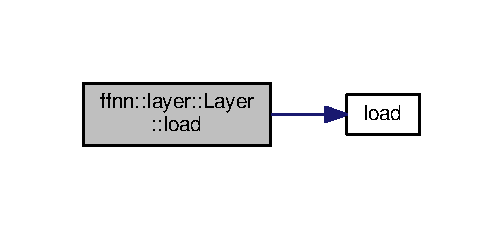
\includegraphics[width=242pt]{classffnn_1_1layer_1_1_layer_a66c56645e54f6e864fb716fdc8858828_cgraph}
\end{center}
\end{figure}


\hypertarget{classffnn_1_1layer_1_1_layer_a5091f6ccef4d80254dd8caf72d13d136}{\index{ffnn\-::layer\-::\-Layer@{ffnn\-::layer\-::\-Layer}!save@{save}}
\index{save@{save}!ffnn::layer::Layer@{ffnn\-::layer\-::\-Layer}}
\subsubsection[{save}]{\setlength{\rightskip}{0pt plus 5cm}template$<$typename Value\-Type, class Enable\-Alignment = std\-::true\-\_\-type$>$ void {\bf ffnn\-::layer\-::\-Layer}$<$ Value\-Type, Enable\-Alignment $>$\-::save (
\begin{DoxyParamCaption}
\item[{{\bf Output\-Archive} \&}]{ar, }
\item[{{\bf Version\-Type}}]{version}
\end{DoxyParamCaption}
) const\hspace{0.3cm}{\ttfamily [protected]}, {\ttfamily [virtual]}}}\label{classffnn_1_1layer_1_1_layer_a5091f6ccef4d80254dd8caf72d13d136}


Save serializer. 



Reimplemented from \hyperlink{classffnn_1_1layer_1_1internal_1_1_interface_a417d6fda112fdffed8091b0ebd78ed97}{ffnn\-::layer\-::internal\-::\-Interface$<$ Value\-Type $>$}.



Here is the call graph for this function\-:
\nopagebreak
\begin{figure}[H]
\begin{center}
\leavevmode
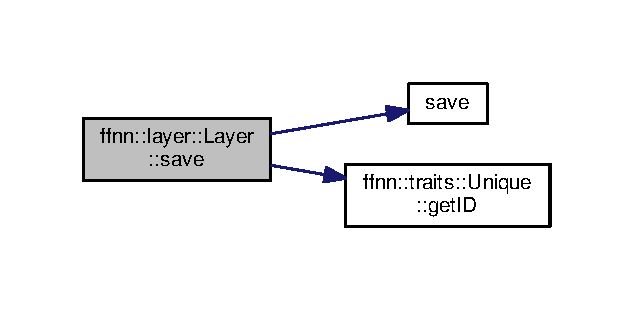
\includegraphics[width=304pt]{classffnn_1_1layer_1_1_layer_a5091f6ccef4d80254dd8caf72d13d136_cgraph}
\end{center}
\end{figure}


\hypertarget{classffnn_1_1layer_1_1_layer_a0e87cf29789204037c4678ee4bfc8756}{\index{ffnn\-::layer\-::\-Layer@{ffnn\-::layer\-::\-Layer}!update@{update}}
\index{update@{update}!ffnn::layer::Layer@{ffnn\-::layer\-::\-Layer}}
\subsubsection[{update}]{\setlength{\rightskip}{0pt plus 5cm}template$<$typename Value\-Type, class Enable\-Alignment = std\-::true\-\_\-type$>$ virtual bool {\bf ffnn\-::layer\-::\-Layer}$<$ Value\-Type, Enable\-Alignment $>$\-::update (
\begin{DoxyParamCaption}
{}
\end{DoxyParamCaption}
)\hspace{0.3cm}{\ttfamily [inline]}, {\ttfamily [virtual]}}}\label{classffnn_1_1layer_1_1_layer_a0e87cf29789204037c4678ee4bfc8756}


Applies layer weight updates. 


\begin{DoxyRetVals}{Return values}
{\em true} & if weight update succeeded \\
\hline
{\em false} & otherwise \\
\hline
\end{DoxyRetVals}


Reimplemented in \hyperlink{classffnn_1_1layer_1_1_convolution_a398b063c5e953e0cb21a827f139a2540}{ffnn\-::layer\-::\-Convolution$<$ Value\-Type, Height\-At\-Compile\-Time, Width\-At\-Compile\-Time, Depth\-At\-Compile\-Time, Filter\-Height\-At\-Compile\-Time, Filter\-Width\-At\-Compile\-Time, Filter\-Count\-At\-Compile\-Time, Stride\-At\-Compile\-Time, Mode $>$}, \hyperlink{classffnn_1_1layer_1_1_sparsely_connected_afa564d528e74917231da2d038f76e3f1}{ffnn\-::layer\-::\-Sparsely\-Connected$<$ Value\-Type, Inputs\-At\-Compile\-Time, Outputs\-At\-Compile\-Time $>$}, \hyperlink{classffnn_1_1layer_1_1_fully_connected_a3194dde96feea7d008cc0c27f30cc805}{ffnn\-::layer\-::\-Fully\-Connected$<$ Value\-Type, Inputs\-At\-Compile\-Time, Outputs\-At\-Compile\-Time $>$}, \hyperlink{classffnn_1_1layer_1_1_hidden_ace039624b0b202413e068fd523f26884}{ffnn\-::layer\-::\-Hidden$<$ Value\-Type, Input\-Height\-At\-Compile\-Time, Input\-Width\-At\-Compile\-Time, Output\-Height\-At\-Compile\-Time, Output\-Width\-At\-Compile\-Time, \-\_\-\-Input\-Block\-Type, \-\_\-\-Output\-Block\-Type, \-\_\-\-Input\-Mapping\-Type, \-\_\-\-Output\-Mapping\-Type $>$}, \hyperlink{classffnn_1_1layer_1_1_hidden_ace039624b0b202413e068fd523f26884}{ffnn\-::layer\-::\-Hidden$<$ Value\-Type, Inputs\-At\-Compile\-Time, 1, Outputs\-At\-Compile\-Time, 1 $>$}, \hyperlink{classffnn_1_1layer_1_1_hidden_ace039624b0b202413e068fd523f26884}{ffnn\-::layer\-::\-Hidden$<$ Value\-Type, Size\-At\-Compile\-Time, 1, Size\-At\-Compile\-Time, 1 $>$}, and \hyperlink{classffnn_1_1layer_1_1_hidden_ace039624b0b202413e068fd523f26884}{ffnn\-::layer\-::\-Hidden$<$ Value\-Type, embed\-\_\-dimension$<$ Mode, Col\-Embedding $>$(\-Height\-At\-Compile\-Time, Depth\-At\-Compile\-Time), embed\-\_\-dimension$<$ Mode, Row\-Embedding $>$(\-Width\-At\-Compile\-Time, Depth\-At\-Compile\-Time), embed\-\_\-dimension$<$ Mode, Col\-Embedding $>$(output\-\_\-dimension(\-Height\-At\-Compile\-Time, Filter\-Height\-At\-Compile\-Time, Stride\-At\-Compile\-Time), Filter\-Count\-At\-Compile\-Time), embed\-\_\-dimension$<$ Mode, Row\-Embedding $>$(output\-\_\-dimension(\-Width\-At\-Compile\-Time, Filter\-Width\-At\-Compile\-Time, Stride\-At\-Compile\-Time), Filter\-Count\-At\-Compile\-Time)$>$}.



\subsection{Friends And Related Function Documentation}
\hypertarget{classffnn_1_1layer_1_1_layer_afbf91ff52dc8c3e894968dcc27cdecd5}{\index{ffnn\-::layer\-::\-Layer@{ffnn\-::layer\-::\-Layer}!connect@{connect}}
\index{connect@{connect}!ffnn::layer::Layer@{ffnn\-::layer\-::\-Layer}}
\subsubsection[{connect}]{\setlength{\rightskip}{0pt plus 5cm}template$<$typename Value\-Type, class Enable\-Alignment = std\-::true\-\_\-type$>$ template$<$typename Layer\-Type $>$ bool connect (
\begin{DoxyParamCaption}
\item[{const typename Layer\-Type\-::\-Ptr \&}]{from, }
\item[{const typename Layer\-Type\-::\-Ptr \&}]{to}
\end{DoxyParamCaption}
)\hspace{0.3cm}{\ttfamily [friend]}}}\label{classffnn_1_1layer_1_1_layer_afbf91ff52dc8c3e894968dcc27cdecd5}


Connects \hyperlink{classffnn_1_1layer_1_1_layer}{Layer} objects. 



\subsection{Member Data Documentation}
\hypertarget{classffnn_1_1layer_1_1_layer_a1be25b9933d64c2964b4260db770ad48}{\index{ffnn\-::layer\-::\-Layer@{ffnn\-::layer\-::\-Layer}!backward\-\_\-error\-\_\-buffer\-\_\-@{backward\-\_\-error\-\_\-buffer\-\_\-}}
\index{backward\-\_\-error\-\_\-buffer\-\_\-@{backward\-\_\-error\-\_\-buffer\-\_\-}!ffnn::layer::Layer@{ffnn\-::layer\-::\-Layer}}
\subsubsection[{backward\-\_\-error\-\_\-buffer\-\_\-}]{\setlength{\rightskip}{0pt plus 5cm}template$<$typename Value\-Type, class Enable\-Alignment = std\-::true\-\_\-type$>$ {\bf Buffer\-Type} {\bf ffnn\-::layer\-::\-Layer}$<$ Value\-Type, Enable\-Alignment $>$\-::backward\-\_\-error\-\_\-buffer\-\_\-\hspace{0.3cm}{\ttfamily [protected]}}}\label{classffnn_1_1layer_1_1_layer_a1be25b9933d64c2964b4260db770ad48}


Raw bakward error value buffer. 



Referenced by ffnn\-::layer\-::\-Layer$<$ Value\-Type $>$\-::get\-Backward\-Error\-Buffer().

\hypertarget{classffnn_1_1layer_1_1_layer_a8595d0898a1530aaec71aec487037655}{\index{ffnn\-::layer\-::\-Layer@{ffnn\-::layer\-::\-Layer}!input\-\_\-buffer\-\_\-@{input\-\_\-buffer\-\_\-}}
\index{input\-\_\-buffer\-\_\-@{input\-\_\-buffer\-\_\-}!ffnn::layer::Layer@{ffnn\-::layer\-::\-Layer}}
\subsubsection[{input\-\_\-buffer\-\_\-}]{\setlength{\rightskip}{0pt plus 5cm}template$<$typename Value\-Type, class Enable\-Alignment = std\-::true\-\_\-type$>$ {\bf Buffer\-Type} {\bf ffnn\-::layer\-::\-Layer}$<$ Value\-Type, Enable\-Alignment $>$\-::input\-\_\-buffer\-\_\-\hspace{0.3cm}{\ttfamily [protected]}}}\label{classffnn_1_1layer_1_1_layer_a8595d0898a1530aaec71aec487037655}


Raw input value buffer. 



Referenced by ffnn\-::layer\-::\-Layer$<$ Value\-Type $>$\-::get\-Input\-Buffer().

\hypertarget{classffnn_1_1layer_1_1_layer_ad665f209da80c13770f2b6a790d3ed4f}{\index{ffnn\-::layer\-::\-Layer@{ffnn\-::layer\-::\-Layer}!prev\-\_\-@{prev\-\_\-}}
\index{prev\-\_\-@{prev\-\_\-}!ffnn::layer::Layer@{ffnn\-::layer\-::\-Layer}}
\subsubsection[{prev\-\_\-}]{\setlength{\rightskip}{0pt plus 5cm}template$<$typename Value\-Type, class Enable\-Alignment = std\-::true\-\_\-type$>$ std\-::map$<$std\-::string, typename {\bf Self\-::\-Ptr}$>$ {\bf ffnn\-::layer\-::\-Layer}$<$ Value\-Type, Enable\-Alignment $>$\-::prev\-\_\-\hspace{0.3cm}{\ttfamily [protected]}}}\label{classffnn_1_1layer_1_1_layer_ad665f209da80c13770f2b6a790d3ed4f}


Pointers to previous layers. 



The documentation for this class was generated from the following files\-:\begin{DoxyCompactItemize}
\item 
/home/briancairl/packages/src/ffnn-\/cpp/ffnn/include/ffnn/layer/\hyperlink{layer_8h}{layer.\-h}\item 
/home/briancairl/packages/src/ffnn-\/cpp/ffnn/include/ffnn/layer/impl/\hyperlink{layer_8hpp}{layer.\-hpp}\end{DoxyCompactItemize}

\hypertarget{classffnn_1_1neuron_1_1_leaky_rectified_linear}{\section{ffnn\-:\-:neuron\-:\-:Leaky\-Rectified\-Linear$<$ Value\-Type, \-\_\-\-P, \-\_\-\-B $>$ Class Template Reference}
\label{classffnn_1_1neuron_1_1_leaky_rectified_linear}\index{ffnn\-::neuron\-::\-Leaky\-Rectified\-Linear$<$ Value\-Type, \-\_\-\-P, \-\_\-\-B $>$@{ffnn\-::neuron\-::\-Leaky\-Rectified\-Linear$<$ Value\-Type, \-\_\-\-P, \-\_\-\-B $>$}}
}


A leaky-\/rectified linear activation unit.  




{\ttfamily \#include \char`\"{}leaky\-\_\-rectified\-\_\-linear.\-h\char`\"{}}



Inheritance diagram for ffnn\-:\-:neuron\-:\-:Leaky\-Rectified\-Linear$<$ Value\-Type, \-\_\-\-P, \-\_\-\-B $>$\-:
\nopagebreak
\begin{figure}[H]
\begin{center}
\leavevmode
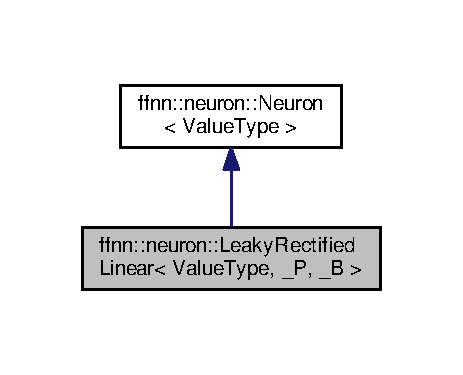
\includegraphics[width=222pt]{classffnn_1_1neuron_1_1_leaky_rectified_linear__inherit__graph}
\end{center}
\end{figure}


Collaboration diagram for ffnn\-:\-:neuron\-:\-:Leaky\-Rectified\-Linear$<$ Value\-Type, \-\_\-\-P, \-\_\-\-B $>$\-:
\nopagebreak
\begin{figure}[H]
\begin{center}
\leavevmode
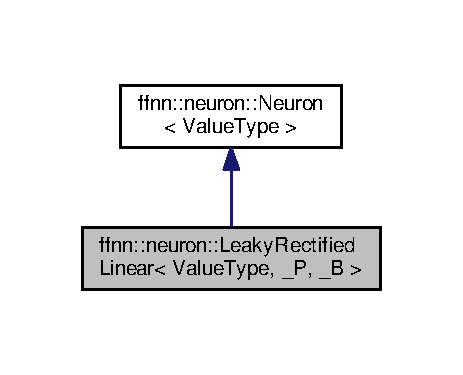
\includegraphics[width=222pt]{classffnn_1_1neuron_1_1_leaky_rectified_linear__coll__graph}
\end{center}
\end{figure}
\subsection*{Public Member Functions}
\begin{DoxyCompactItemize}
\item 
\hyperlink{classffnn_1_1neuron_1_1_leaky_rectified_linear_aedaef89cf5a9390b4ec610d1e7157bf8}{Leaky\-Rectified\-Linear} ()
\begin{DoxyCompactList}\small\item\em Setup constructor. \end{DoxyCompactList}\item 
virtual void \hyperlink{classffnn_1_1neuron_1_1_leaky_rectified_linear_a6a96858235a3c4a8195b27699032a849}{fn} (const Value\-Type \&input, Value\-Type \&output)
\begin{DoxyCompactList}\small\item\em Computes activation output. \end{DoxyCompactList}\item 
virtual void \hyperlink{classffnn_1_1neuron_1_1_leaky_rectified_linear_a1bb98dd03e854a69a7ba76b347ec4340}{derivative} (const Value\-Type \&input, Value\-Type \&output) const 
\begin{DoxyCompactList}\small\item\em Computes first-\/order activation derivative. \end{DoxyCompactList}\end{DoxyCompactItemize}
\subsection*{Protected Attributes}
\begin{DoxyCompactItemize}
\item 
const Value\-Type \hyperlink{classffnn_1_1neuron_1_1_leaky_rectified_linear_ab205c35e3123e8965efe63cd665020cb}{leak\-\_\-factor\-\_\-}
\begin{DoxyCompactList}\small\item\em Factor in the range \mbox{[}0, 1\mbox{]} to leak when (input $<$ 0) \end{DoxyCompactList}\end{DoxyCompactItemize}


\subsection{Detailed Description}
\subsubsection*{template$<$typename Value\-Type, F\-F\-N\-N\-\_\-\-S\-I\-Z\-E\-\_\-\-T\-Y\-P\-E \-\_\-\-P, F\-F\-N\-N\-\_\-\-S\-I\-Z\-E\-\_\-\-T\-Y\-P\-E \-\_\-\-B = 100$>$class ffnn\-::neuron\-::\-Leaky\-Rectified\-Linear$<$ Value\-Type, \-\_\-\-P, \-\_\-\-B $>$}

A leaky-\/rectified linear activation unit. 

\subsection{Constructor \& Destructor Documentation}
\hypertarget{classffnn_1_1neuron_1_1_leaky_rectified_linear_aedaef89cf5a9390b4ec610d1e7157bf8}{\index{ffnn\-::neuron\-::\-Leaky\-Rectified\-Linear@{ffnn\-::neuron\-::\-Leaky\-Rectified\-Linear}!Leaky\-Rectified\-Linear@{Leaky\-Rectified\-Linear}}
\index{Leaky\-Rectified\-Linear@{Leaky\-Rectified\-Linear}!ffnn::neuron::LeakyRectifiedLinear@{ffnn\-::neuron\-::\-Leaky\-Rectified\-Linear}}
\subsubsection[{Leaky\-Rectified\-Linear}]{\setlength{\rightskip}{0pt plus 5cm}template$<$typename Value\-Type , F\-F\-N\-N\-\_\-\-S\-I\-Z\-E\-\_\-\-T\-Y\-P\-E \-\_\-\-P, F\-F\-N\-N\-\_\-\-S\-I\-Z\-E\-\_\-\-T\-Y\-P\-E \-\_\-\-B = 100$>$ {\bf ffnn\-::neuron\-::\-Leaky\-Rectified\-Linear}$<$ Value\-Type, \-\_\-\-P, \-\_\-\-B $>$\-::{\bf Leaky\-Rectified\-Linear} (
\begin{DoxyParamCaption}
{}
\end{DoxyParamCaption}
)\hspace{0.3cm}{\ttfamily [inline]}}}\label{classffnn_1_1neuron_1_1_leaky_rectified_linear_aedaef89cf5a9390b4ec610d1e7157bf8}


Setup constructor. 


\begin{DoxyParams}{Parameters}
{\em leak\-\_\-factor} & input to leak with (input $<$ 0) \\
\hline
\end{DoxyParams}


\subsection{Member Function Documentation}
\hypertarget{classffnn_1_1neuron_1_1_leaky_rectified_linear_a1bb98dd03e854a69a7ba76b347ec4340}{\index{ffnn\-::neuron\-::\-Leaky\-Rectified\-Linear@{ffnn\-::neuron\-::\-Leaky\-Rectified\-Linear}!derivative@{derivative}}
\index{derivative@{derivative}!ffnn::neuron::LeakyRectifiedLinear@{ffnn\-::neuron\-::\-Leaky\-Rectified\-Linear}}
\subsubsection[{derivative}]{\setlength{\rightskip}{0pt plus 5cm}template$<$typename Value\-Type , F\-F\-N\-N\-\_\-\-S\-I\-Z\-E\-\_\-\-T\-Y\-P\-E \-\_\-\-P, F\-F\-N\-N\-\_\-\-S\-I\-Z\-E\-\_\-\-T\-Y\-P\-E \-\_\-\-B = 100$>$ virtual void {\bf ffnn\-::neuron\-::\-Leaky\-Rectified\-Linear}$<$ Value\-Type, \-\_\-\-P, \-\_\-\-B $>$\-::derivative (
\begin{DoxyParamCaption}
\item[{const Value\-Type \&}]{input, }
\item[{Value\-Type \&}]{output}
\end{DoxyParamCaption}
) const\hspace{0.3cm}{\ttfamily [inline]}, {\ttfamily [virtual]}}}\label{classffnn_1_1neuron_1_1_leaky_rectified_linear_a1bb98dd03e854a69a7ba76b347ec4340}


Computes first-\/order activation derivative. 


\begin{DoxyParams}[1]{Parameters}
\mbox{\tt in}  & {\em input} & a scalar input value \\
\hline
\mbox{\tt in,out}  & {\em output} & a scalar output value \\
\hline
\end{DoxyParams}


Implements \hyperlink{classffnn_1_1neuron_1_1_neuron_ac779b179887e6b4505dec96d0319af10}{ffnn\-::neuron\-::\-Neuron$<$ Value\-Type $>$}.

\hypertarget{classffnn_1_1neuron_1_1_leaky_rectified_linear_a6a96858235a3c4a8195b27699032a849}{\index{ffnn\-::neuron\-::\-Leaky\-Rectified\-Linear@{ffnn\-::neuron\-::\-Leaky\-Rectified\-Linear}!fn@{fn}}
\index{fn@{fn}!ffnn::neuron::LeakyRectifiedLinear@{ffnn\-::neuron\-::\-Leaky\-Rectified\-Linear}}
\subsubsection[{fn}]{\setlength{\rightskip}{0pt plus 5cm}template$<$typename Value\-Type , F\-F\-N\-N\-\_\-\-S\-I\-Z\-E\-\_\-\-T\-Y\-P\-E \-\_\-\-P, F\-F\-N\-N\-\_\-\-S\-I\-Z\-E\-\_\-\-T\-Y\-P\-E \-\_\-\-B = 100$>$ virtual void {\bf ffnn\-::neuron\-::\-Leaky\-Rectified\-Linear}$<$ Value\-Type, \-\_\-\-P, \-\_\-\-B $>$\-::fn (
\begin{DoxyParamCaption}
\item[{const Value\-Type \&}]{input, }
\item[{Value\-Type \&}]{output}
\end{DoxyParamCaption}
)\hspace{0.3cm}{\ttfamily [inline]}, {\ttfamily [virtual]}}}\label{classffnn_1_1neuron_1_1_leaky_rectified_linear_a6a96858235a3c4a8195b27699032a849}


Computes activation output. 


\begin{DoxyParams}[1]{Parameters}
\mbox{\tt in}  & {\em input} & a scalar input value \\
\hline
\mbox{\tt in,out}  & {\em output} & a scalar output value \\
\hline
\end{DoxyParams}


Implements \hyperlink{classffnn_1_1neuron_1_1_neuron_a4f03bb4fe57ffa74d70e447237b9b8fb}{ffnn\-::neuron\-::\-Neuron$<$ Value\-Type $>$}.



\subsection{Member Data Documentation}
\hypertarget{classffnn_1_1neuron_1_1_leaky_rectified_linear_ab205c35e3123e8965efe63cd665020cb}{\index{ffnn\-::neuron\-::\-Leaky\-Rectified\-Linear@{ffnn\-::neuron\-::\-Leaky\-Rectified\-Linear}!leak\-\_\-factor\-\_\-@{leak\-\_\-factor\-\_\-}}
\index{leak\-\_\-factor\-\_\-@{leak\-\_\-factor\-\_\-}!ffnn::neuron::LeakyRectifiedLinear@{ffnn\-::neuron\-::\-Leaky\-Rectified\-Linear}}
\subsubsection[{leak\-\_\-factor\-\_\-}]{\setlength{\rightskip}{0pt plus 5cm}template$<$typename Value\-Type , F\-F\-N\-N\-\_\-\-S\-I\-Z\-E\-\_\-\-T\-Y\-P\-E \-\_\-\-P, F\-F\-N\-N\-\_\-\-S\-I\-Z\-E\-\_\-\-T\-Y\-P\-E \-\_\-\-B = 100$>$ const Value\-Type {\bf ffnn\-::neuron\-::\-Leaky\-Rectified\-Linear}$<$ Value\-Type, \-\_\-\-P, \-\_\-\-B $>$\-::leak\-\_\-factor\-\_\-\hspace{0.3cm}{\ttfamily [protected]}}}\label{classffnn_1_1neuron_1_1_leaky_rectified_linear_ab205c35e3123e8965efe63cd665020cb}


Factor in the range \mbox{[}0, 1\mbox{]} to leak when (input $<$ 0) 



Referenced by ffnn\-::neuron\-::\-Leaky\-Rectified\-Linear$<$ Value\-Type, \-\_\-\-P, \-\_\-\-B $>$\-::derivative(), ffnn\-::neuron\-::\-Leaky\-Rectified\-Linear$<$ Value\-Type, \-\_\-\-P, \-\_\-\-B $>$\-::fn(), and ffnn\-::neuron\-::\-Leaky\-Rectified\-Linear$<$ Value\-Type, \-\_\-\-P, \-\_\-\-B $>$\-::\-Leaky\-Rectified\-Linear().



The documentation for this class was generated from the following file\-:\begin{DoxyCompactItemize}
\item 
/home/briancairl/packages/src/ffnn-\/cpp/ffnn/include/ffnn/neuron/\hyperlink{leaky__rectified__linear_8h}{leaky\-\_\-rectified\-\_\-linear.\-h}\end{DoxyCompactItemize}

\hypertarget{classffnn_1_1neuron_1_1_le_cun_sigmoid}{\section{ffnn\-:\-:neuron\-:\-:Le\-Cun\-Sigmoid$<$ Value\-Type $>$ Class Template Reference}
\label{classffnn_1_1neuron_1_1_le_cun_sigmoid}\index{ffnn\-::neuron\-::\-Le\-Cun\-Sigmoid$<$ Value\-Type $>$@{ffnn\-::neuron\-::\-Le\-Cun\-Sigmoid$<$ Value\-Type $>$}}
}


A bipolar sigmoid activation unit scaled to prevent saturation.  




{\ttfamily \#include \char`\"{}lecun\-\_\-sigmoid.\-h\char`\"{}}



Inheritance diagram for ffnn\-:\-:neuron\-:\-:Le\-Cun\-Sigmoid$<$ Value\-Type $>$\-:\nopagebreak
\begin{figure}[H]
\begin{center}
\leavevmode
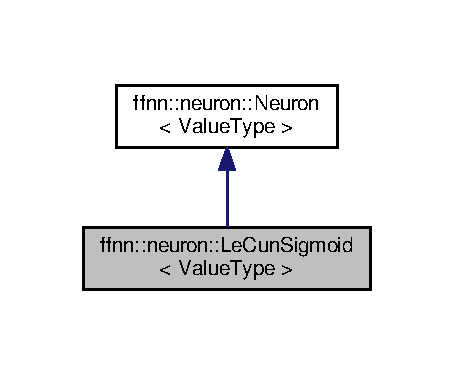
\includegraphics[width=218pt]{classffnn_1_1neuron_1_1_le_cun_sigmoid__inherit__graph}
\end{center}
\end{figure}


Collaboration diagram for ffnn\-:\-:neuron\-:\-:Le\-Cun\-Sigmoid$<$ Value\-Type $>$\-:\nopagebreak
\begin{figure}[H]
\begin{center}
\leavevmode
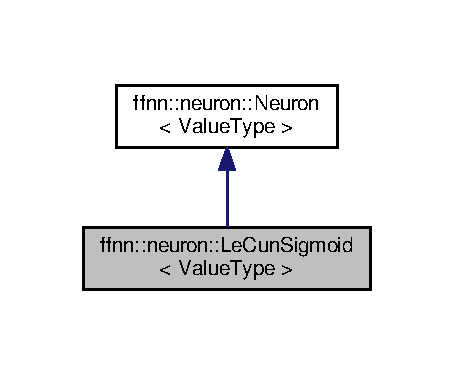
\includegraphics[width=218pt]{classffnn_1_1neuron_1_1_le_cun_sigmoid__coll__graph}
\end{center}
\end{figure}
\subsection*{Public Member Functions}
\begin{DoxyCompactItemize}
\item 
virtual void \hyperlink{classffnn_1_1neuron_1_1_le_cun_sigmoid_ae1a0a4b086a8983f31fb320e7c3088dc}{operator()} (const Value\-Type \&input, Value\-Type \&output)
\begin{DoxyCompactList}\small\item\em Computes activation output. \end{DoxyCompactList}\item 
virtual void \hyperlink{classffnn_1_1neuron_1_1_le_cun_sigmoid_a4802deb108ab8ca6a67a4d7d55124fb2}{derivative} (const Value\-Type \&input, Value\-Type \&output) const 
\begin{DoxyCompactList}\small\item\em Computes first-\/order activation derivative. \end{DoxyCompactList}\end{DoxyCompactItemize}
\subsection*{Additional Inherited Members}


\subsection{Detailed Description}
\subsubsection*{template$<$typename Value\-Type$>$class ffnn\-::neuron\-::\-Le\-Cun\-Sigmoid$<$ Value\-Type $>$}

A bipolar sigmoid activation unit scaled to prevent saturation. 

Represents the mapping \[ f(x) = 1.7159 * tanh(2/3 x) \]

\begin{DoxyNote}{Note}
ref\-: \href{http://yann.lecun.com/exdb/publis/pdf/lecun-98b.pdf}{\tt http\-://yann.\-lecun.\-com/exdb/publis/pdf/lecun-\/98b.\-pdf} 
\end{DoxyNote}


\subsection{Member Function Documentation}
\hypertarget{classffnn_1_1neuron_1_1_le_cun_sigmoid_a4802deb108ab8ca6a67a4d7d55124fb2}{\index{ffnn\-::neuron\-::\-Le\-Cun\-Sigmoid@{ffnn\-::neuron\-::\-Le\-Cun\-Sigmoid}!derivative@{derivative}}
\index{derivative@{derivative}!ffnn::neuron::LeCunSigmoid@{ffnn\-::neuron\-::\-Le\-Cun\-Sigmoid}}
\subsubsection[{derivative}]{\setlength{\rightskip}{0pt plus 5cm}template$<$typename Value\-Type $>$ virtual void {\bf ffnn\-::neuron\-::\-Le\-Cun\-Sigmoid}$<$ Value\-Type $>$\-::derivative (
\begin{DoxyParamCaption}
\item[{const Value\-Type \&}]{input, }
\item[{Value\-Type \&}]{output}
\end{DoxyParamCaption}
) const\hspace{0.3cm}{\ttfamily [inline]}, {\ttfamily [virtual]}}}\label{classffnn_1_1neuron_1_1_le_cun_sigmoid_a4802deb108ab8ca6a67a4d7d55124fb2}


Computes first-\/order activation derivative. 


\begin{DoxyParams}[1]{Parameters}
\mbox{\tt in}  & {\em input} & a scalar input value \\
\hline
\mbox{\tt in,out}  & {\em output} & a scalar output value \\
\hline
\end{DoxyParams}


Implements \hyperlink{classffnn_1_1neuron_1_1_neuron_ac779b179887e6b4505dec96d0319af10}{ffnn\-::neuron\-::\-Neuron$<$ Value\-Type $>$}.

\hypertarget{classffnn_1_1neuron_1_1_le_cun_sigmoid_ae1a0a4b086a8983f31fb320e7c3088dc}{\index{ffnn\-::neuron\-::\-Le\-Cun\-Sigmoid@{ffnn\-::neuron\-::\-Le\-Cun\-Sigmoid}!operator()@{operator()}}
\index{operator()@{operator()}!ffnn::neuron::LeCunSigmoid@{ffnn\-::neuron\-::\-Le\-Cun\-Sigmoid}}
\subsubsection[{operator()}]{\setlength{\rightskip}{0pt plus 5cm}template$<$typename Value\-Type $>$ virtual void {\bf ffnn\-::neuron\-::\-Le\-Cun\-Sigmoid}$<$ Value\-Type $>$\-::operator() (
\begin{DoxyParamCaption}
\item[{const Value\-Type \&}]{input, }
\item[{Value\-Type \&}]{output}
\end{DoxyParamCaption}
)\hspace{0.3cm}{\ttfamily [inline]}, {\ttfamily [virtual]}}}\label{classffnn_1_1neuron_1_1_le_cun_sigmoid_ae1a0a4b086a8983f31fb320e7c3088dc}


Computes activation output. 


\begin{DoxyParams}[1]{Parameters}
\mbox{\tt in}  & {\em input} & a scalar input value \\
\hline
\mbox{\tt in,out}  & {\em output} & a scalar output value \\
\hline
\end{DoxyParams}


Implements \hyperlink{classffnn_1_1neuron_1_1_neuron_ae215373ce29e135cb5fd728964772a32}{ffnn\-::neuron\-::\-Neuron$<$ Value\-Type $>$}.



The documentation for this class was generated from the following file\-:\begin{DoxyCompactItemize}
\item 
/home/briancairl/packages/src/ffnn-\/cpp/ffnn/include/ffnn/neuron/\hyperlink{lecun__sigmoid_8h}{lecun\-\_\-sigmoid.\-h}\end{DoxyCompactItemize}

\hypertarget{classffnn_1_1neuron_1_1_linear}{\section{ffnn\-:\-:neuron\-:\-:Linear$<$ Value\-Type $>$ Class Template Reference}
\label{classffnn_1_1neuron_1_1_linear}\index{ffnn\-::neuron\-::\-Linear$<$ Value\-Type $>$@{ffnn\-::neuron\-::\-Linear$<$ Value\-Type $>$}}
}


A linear activation unit.  




{\ttfamily \#include \char`\"{}linear.\-h\char`\"{}}



Inheritance diagram for ffnn\-:\-:neuron\-:\-:Linear$<$ Value\-Type $>$\-:\nopagebreak
\begin{figure}[H]
\begin{center}
\leavevmode
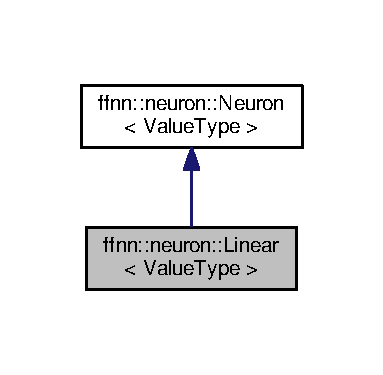
\includegraphics[width=184pt]{classffnn_1_1neuron_1_1_linear__inherit__graph}
\end{center}
\end{figure}


Collaboration diagram for ffnn\-:\-:neuron\-:\-:Linear$<$ Value\-Type $>$\-:\nopagebreak
\begin{figure}[H]
\begin{center}
\leavevmode
\includegraphics[width=184pt]{classffnn_1_1neuron_1_1_linear__coll__graph}
\end{center}
\end{figure}
\subsection*{Public Member Functions}
\begin{DoxyCompactItemize}
\item 
virtual void \hyperlink{classffnn_1_1neuron_1_1_linear_a4d92b666c3e0a81865be7d09c0c4016e}{fn} (const Value\-Type \&input, Value\-Type \&output)
\begin{DoxyCompactList}\small\item\em Computes activation output. \end{DoxyCompactList}\item 
virtual void \hyperlink{classffnn_1_1neuron_1_1_linear_a4656398d6a4c1bda77d25adbad148ae9}{derivative} (const Value\-Type \&input, Value\-Type \&output) const 
\begin{DoxyCompactList}\small\item\em Computes first-\/order activation derivative. \end{DoxyCompactList}\end{DoxyCompactItemize}


\subsection{Detailed Description}
\subsubsection*{template$<$typename Value\-Type$>$class ffnn\-::neuron\-::\-Linear$<$ Value\-Type $>$}

A linear activation unit. 

Represents the mapping \[ f(x) = x \] 

\subsection{Member Function Documentation}
\hypertarget{classffnn_1_1neuron_1_1_linear_a4656398d6a4c1bda77d25adbad148ae9}{\index{ffnn\-::neuron\-::\-Linear@{ffnn\-::neuron\-::\-Linear}!derivative@{derivative}}
\index{derivative@{derivative}!ffnn::neuron::Linear@{ffnn\-::neuron\-::\-Linear}}
\subsubsection[{derivative}]{\setlength{\rightskip}{0pt plus 5cm}template$<$typename Value\-Type $>$ virtual void {\bf ffnn\-::neuron\-::\-Linear}$<$ Value\-Type $>$\-::derivative (
\begin{DoxyParamCaption}
\item[{const Value\-Type \&}]{input, }
\item[{Value\-Type \&}]{output}
\end{DoxyParamCaption}
) const\hspace{0.3cm}{\ttfamily [inline]}, {\ttfamily [virtual]}}}\label{classffnn_1_1neuron_1_1_linear_a4656398d6a4c1bda77d25adbad148ae9}


Computes first-\/order activation derivative. 


\begin{DoxyParams}[1]{Parameters}
\mbox{\tt in}  & {\em input} & a scalar input value \\
\hline
\mbox{\tt in,out}  & {\em output} & a scalar output value \\
\hline
\end{DoxyParams}


Implements \hyperlink{classffnn_1_1neuron_1_1_neuron_ac779b179887e6b4505dec96d0319af10}{ffnn\-::neuron\-::\-Neuron$<$ Value\-Type $>$}.

\hypertarget{classffnn_1_1neuron_1_1_linear_a4d92b666c3e0a81865be7d09c0c4016e}{\index{ffnn\-::neuron\-::\-Linear@{ffnn\-::neuron\-::\-Linear}!fn@{fn}}
\index{fn@{fn}!ffnn::neuron::Linear@{ffnn\-::neuron\-::\-Linear}}
\subsubsection[{fn}]{\setlength{\rightskip}{0pt plus 5cm}template$<$typename Value\-Type $>$ virtual void {\bf ffnn\-::neuron\-::\-Linear}$<$ Value\-Type $>$\-::fn (
\begin{DoxyParamCaption}
\item[{const Value\-Type \&}]{input, }
\item[{Value\-Type \&}]{output}
\end{DoxyParamCaption}
)\hspace{0.3cm}{\ttfamily [inline]}, {\ttfamily [virtual]}}}\label{classffnn_1_1neuron_1_1_linear_a4d92b666c3e0a81865be7d09c0c4016e}


Computes activation output. 


\begin{DoxyParams}[1]{Parameters}
\mbox{\tt in}  & {\em input} & a scalar input value \\
\hline
\mbox{\tt in,out}  & {\em output} & a scalar output value \\
\hline
\end{DoxyParams}


Implements \hyperlink{classffnn_1_1neuron_1_1_neuron_a4f03bb4fe57ffa74d70e447237b9b8fb}{ffnn\-::neuron\-::\-Neuron$<$ Value\-Type $>$}.



The documentation for this class was generated from the following file\-:\begin{DoxyCompactItemize}
\item 
/home/briancairl/packages/src/ffnn-\/cpp/ffnn/include/ffnn/neuron/\hyperlink{linear_8h}{linear.\-h}\end{DoxyCompactItemize}

\hypertarget{classffnn_1_1neuron_1_1_neuron}{\section{ffnn\-:\-:neuron\-:\-:Neuron$<$ Value\-Type $>$ Class Template Reference}
\label{classffnn_1_1neuron_1_1_neuron}\index{ffnn\-::neuron\-::\-Neuron$<$ Value\-Type $>$@{ffnn\-::neuron\-::\-Neuron$<$ Value\-Type $>$}}
}


A basic activation unit type.  




{\ttfamily \#include \char`\"{}neuron.\-h\char`\"{}}



Inheritance diagram for ffnn\-:\-:neuron\-:\-:Neuron$<$ Value\-Type $>$\-:\nopagebreak
\begin{figure}[H]
\begin{center}
\leavevmode
\includegraphics[width=350pt]{classffnn_1_1neuron_1_1_neuron__inherit__graph}
\end{center}
\end{figure}
\subsection*{Public Types}
\begin{DoxyCompactItemize}
\item 
typedef Value\-Type \hyperlink{classffnn_1_1neuron_1_1_neuron_a5c758fa2e21a6dc3de42b34016b93d56}{Scalar}
\end{DoxyCompactItemize}
\subsection*{Public Member Functions}
\begin{DoxyCompactItemize}
\item 
virtual void \hyperlink{classffnn_1_1neuron_1_1_neuron_ae215373ce29e135cb5fd728964772a32}{operator()} (const Value\-Type \&input, Value\-Type \&output)=0
\begin{DoxyCompactList}\small\item\em Computes activation output. \end{DoxyCompactList}\item 
virtual void \hyperlink{classffnn_1_1neuron_1_1_neuron_ac779b179887e6b4505dec96d0319af10}{derivative} (const Value\-Type \&input, Value\-Type \&output) const =0
\begin{DoxyCompactList}\small\item\em Computes first-\/order activation derivative. \end{DoxyCompactList}\end{DoxyCompactItemize}


\subsection{Detailed Description}
\subsubsection*{template$<$typename Value\-Type$>$class ffnn\-::neuron\-::\-Neuron$<$ Value\-Type $>$}

A basic activation unit type. 

\subsection{Member Typedef Documentation}
\hypertarget{classffnn_1_1neuron_1_1_neuron_a5c758fa2e21a6dc3de42b34016b93d56}{\index{ffnn\-::neuron\-::\-Neuron@{ffnn\-::neuron\-::\-Neuron}!Scalar@{Scalar}}
\index{Scalar@{Scalar}!ffnn::neuron::Neuron@{ffnn\-::neuron\-::\-Neuron}}
\subsubsection[{Scalar}]{\setlength{\rightskip}{0pt plus 5cm}template$<$typename Value\-Type $>$ typedef Value\-Type {\bf ffnn\-::neuron\-::\-Neuron}$<$ Value\-Type $>$\-::{\bf Scalar}}}\label{classffnn_1_1neuron_1_1_neuron_a5c758fa2e21a6dc3de42b34016b93d56}


\subsection{Member Function Documentation}
\hypertarget{classffnn_1_1neuron_1_1_neuron_ac779b179887e6b4505dec96d0319af10}{\index{ffnn\-::neuron\-::\-Neuron@{ffnn\-::neuron\-::\-Neuron}!derivative@{derivative}}
\index{derivative@{derivative}!ffnn::neuron::Neuron@{ffnn\-::neuron\-::\-Neuron}}
\subsubsection[{derivative}]{\setlength{\rightskip}{0pt plus 5cm}template$<$typename Value\-Type $>$ virtual void {\bf ffnn\-::neuron\-::\-Neuron}$<$ Value\-Type $>$\-::derivative (
\begin{DoxyParamCaption}
\item[{const Value\-Type \&}]{input, }
\item[{Value\-Type \&}]{output}
\end{DoxyParamCaption}
) const\hspace{0.3cm}{\ttfamily [pure virtual]}}}\label{classffnn_1_1neuron_1_1_neuron_ac779b179887e6b4505dec96d0319af10}


Computes first-\/order activation derivative. 


\begin{DoxyParams}[1]{Parameters}
\mbox{\tt in}  & {\em input} & a scalar input value \\
\hline
\mbox{\tt in,out}  & {\em output} & a scalar output value \\
\hline
\end{DoxyParams}


Implemented in \hyperlink{classffnn_1_1neuron_1_1_leaky_rectified_linear_a1bb98dd03e854a69a7ba76b347ec4340}{ffnn\-::neuron\-::\-Leaky\-Rectified\-Linear$<$ Value\-Type, \-\_\-\-P, \-\_\-\-B $>$}, \hyperlink{classffnn_1_1neuron_1_1_le_cun_sigmoid_a4802deb108ab8ca6a67a4d7d55124fb2}{ffnn\-::neuron\-::\-Le\-Cun\-Sigmoid$<$ Value\-Type $>$}, \hyperlink{classffnn_1_1neuron_1_1_sigmoid_aee2a196924df30414539d75caa6c7030}{ffnn\-::neuron\-::\-Sigmoid$<$ Value\-Type $>$}, \hyperlink{classffnn_1_1neuron_1_1_soft_sign_a1284d2661377557e782547613e299736}{ffnn\-::neuron\-::\-Soft\-Sign$<$ Value\-Type $>$}, \hyperlink{classffnn_1_1neuron_1_1_linear_a4656398d6a4c1bda77d25adbad148ae9}{ffnn\-::neuron\-::\-Linear$<$ Value\-Type $>$}, and \hyperlink{classffnn_1_1neuron_1_1_rectified_linear_a8c45f64142bf994a96f4987cdd81e32f}{ffnn\-::neuron\-::\-Rectified\-Linear$<$ Value\-Type $>$}.

\hypertarget{classffnn_1_1neuron_1_1_neuron_ae215373ce29e135cb5fd728964772a32}{\index{ffnn\-::neuron\-::\-Neuron@{ffnn\-::neuron\-::\-Neuron}!operator()@{operator()}}
\index{operator()@{operator()}!ffnn::neuron::Neuron@{ffnn\-::neuron\-::\-Neuron}}
\subsubsection[{operator()}]{\setlength{\rightskip}{0pt plus 5cm}template$<$typename Value\-Type $>$ virtual void {\bf ffnn\-::neuron\-::\-Neuron}$<$ Value\-Type $>$\-::operator() (
\begin{DoxyParamCaption}
\item[{const Value\-Type \&}]{input, }
\item[{Value\-Type \&}]{output}
\end{DoxyParamCaption}
)\hspace{0.3cm}{\ttfamily [pure virtual]}}}\label{classffnn_1_1neuron_1_1_neuron_ae215373ce29e135cb5fd728964772a32}


Computes activation output. 


\begin{DoxyParams}[1]{Parameters}
\mbox{\tt in}  & {\em input} & a scalar input value \\
\hline
\mbox{\tt in,out}  & {\em output} & a scalar output value \\
\hline
\end{DoxyParams}


Implemented in \hyperlink{classffnn_1_1neuron_1_1_leaky_rectified_linear_a219673d306064ae1405dd9385f031380}{ffnn\-::neuron\-::\-Leaky\-Rectified\-Linear$<$ Value\-Type, \-\_\-\-P, \-\_\-\-B $>$}, \hyperlink{classffnn_1_1neuron_1_1_le_cun_sigmoid_ae1a0a4b086a8983f31fb320e7c3088dc}{ffnn\-::neuron\-::\-Le\-Cun\-Sigmoid$<$ Value\-Type $>$}, \hyperlink{classffnn_1_1neuron_1_1_sigmoid_a1176976ca74341daac6c1720f7056d39}{ffnn\-::neuron\-::\-Sigmoid$<$ Value\-Type $>$}, \hyperlink{classffnn_1_1neuron_1_1_soft_sign_a1d3ecb32d2eeea06b988ef4f779303e0}{ffnn\-::neuron\-::\-Soft\-Sign$<$ Value\-Type $>$}, \hyperlink{classffnn_1_1neuron_1_1_linear_aa59814449ab3e63d2cbd4f01fd500044}{ffnn\-::neuron\-::\-Linear$<$ Value\-Type $>$}, and \hyperlink{classffnn_1_1neuron_1_1_rectified_linear_a11584934d68646ccced2c0c1c382960d}{ffnn\-::neuron\-::\-Rectified\-Linear$<$ Value\-Type $>$}.



The documentation for this class was generated from the following file\-:\begin{DoxyCompactItemize}
\item 
/home/briancairl/packages/src/ffnn-\/cpp/ffnn/include/ffnn/neuron/\hyperlink{neuron_8h}{neuron.\-h}\end{DoxyCompactItemize}

\hypertarget{classffnn_1_1optimizer_1_1_none}{\section{ffnn\-:\-:optimizer\-:\-:None$<$ Layer\-Type $>$ Class Template Reference}
\label{classffnn_1_1optimizer_1_1_none}\index{ffnn\-::optimizer\-::\-None$<$ Layer\-Type $>$@{ffnn\-::optimizer\-::\-None$<$ Layer\-Type $>$}}
}


{\ttfamily \#include \char`\"{}fwd.\-h\char`\"{}}



Inheritance diagram for ffnn\-:\-:optimizer\-:\-:None$<$ Layer\-Type $>$\-:\nopagebreak
\begin{figure}[H]
\begin{center}
\leavevmode
\includegraphics[width=206pt]{classffnn_1_1optimizer_1_1_none__inherit__graph}
\end{center}
\end{figure}


Collaboration diagram for ffnn\-:\-:optimizer\-:\-:None$<$ Layer\-Type $>$\-:\nopagebreak
\begin{figure}[H]
\begin{center}
\leavevmode
\includegraphics[width=206pt]{classffnn_1_1optimizer_1_1_none__coll__graph}
\end{center}
\end{figure}
\subsection*{Public Member Functions}
\begin{DoxyCompactItemize}
\item 
\hyperlink{classffnn_1_1optimizer_1_1_none_ae5ba72205a7f11508de871d6c3f1081f}{None} ()
\begin{DoxyCompactList}\small\item\em Default constructor. \end{DoxyCompactList}\item 
virtual \hyperlink{classffnn_1_1optimizer_1_1_none_a7e7dc203e5e857d44e1335ba9aac3711}{$\sim$\-None} ()
\item 
void \hyperlink{classffnn_1_1optimizer_1_1_none_a976eb3fe07f8c23a81851e7af4169ec8}{initialize} (Layer\-Type \&layer)
\begin{DoxyCompactList}\small\item\em Passthrough. \end{DoxyCompactList}\item 
void \hyperlink{classffnn_1_1optimizer_1_1_none_a10f714488a57b139b91a03939a8809ac}{reset} (Layer\-Type \&layer)
\begin{DoxyCompactList}\small\item\em Passthrough. \end{DoxyCompactList}\item 
bool \hyperlink{classffnn_1_1optimizer_1_1_none_a4aa65aa33dc45fa3b5d30e7f2a7169f2}{forward} (Layer\-Type \&layer)
\begin{DoxyCompactList}\small\item\em Passthrough. \end{DoxyCompactList}\item 
bool \hyperlink{classffnn_1_1optimizer_1_1_none_a1b8fb0b29f3f0afccc557f6b486fb3fe}{backward} (Layer\-Type \&layer)
\begin{DoxyCompactList}\small\item\em Does nothing. \end{DoxyCompactList}\item 
bool \hyperlink{classffnn_1_1optimizer_1_1_none_aa2d59b906b49fb976b50a810479637fd}{update} (Layer\-Type \&layer)
\begin{DoxyCompactList}\small\item\em Does nothing. \end{DoxyCompactList}\end{DoxyCompactItemize}
\subsection*{Additional Inherited Members}


\subsection{Constructor \& Destructor Documentation}
\hypertarget{classffnn_1_1optimizer_1_1_none_ae5ba72205a7f11508de871d6c3f1081f}{\index{ffnn\-::optimizer\-::\-None@{ffnn\-::optimizer\-::\-None}!None@{None}}
\index{None@{None}!ffnn::optimizer::None@{ffnn\-::optimizer\-::\-None}}
\subsubsection[{None}]{\setlength{\rightskip}{0pt plus 5cm}template$<$typename Layer\-Type $>$ {\bf ffnn\-::optimizer\-::\-None}$<$ Layer\-Type $>$\-::{\bf None} (
\begin{DoxyParamCaption}
{}
\end{DoxyParamCaption}
)\hspace{0.3cm}{\ttfamily [inline]}}}\label{classffnn_1_1optimizer_1_1_none_ae5ba72205a7f11508de871d6c3f1081f}


Default constructor. 

\hypertarget{classffnn_1_1optimizer_1_1_none_a7e7dc203e5e857d44e1335ba9aac3711}{\index{ffnn\-::optimizer\-::\-None@{ffnn\-::optimizer\-::\-None}!$\sim$\-None@{$\sim$\-None}}
\index{$\sim$\-None@{$\sim$\-None}!ffnn::optimizer::None@{ffnn\-::optimizer\-::\-None}}
\subsubsection[{$\sim$\-None}]{\setlength{\rightskip}{0pt plus 5cm}template$<$typename Layer\-Type $>$ virtual {\bf ffnn\-::optimizer\-::\-None}$<$ Layer\-Type $>$\-::$\sim${\bf None} (
\begin{DoxyParamCaption}
{}
\end{DoxyParamCaption}
)\hspace{0.3cm}{\ttfamily [inline]}, {\ttfamily [virtual]}}}\label{classffnn_1_1optimizer_1_1_none_a7e7dc203e5e857d44e1335ba9aac3711}


\subsection{Member Function Documentation}
\hypertarget{classffnn_1_1optimizer_1_1_none_a1b8fb0b29f3f0afccc557f6b486fb3fe}{\index{ffnn\-::optimizer\-::\-None@{ffnn\-::optimizer\-::\-None}!backward@{backward}}
\index{backward@{backward}!ffnn::optimizer::None@{ffnn\-::optimizer\-::\-None}}
\subsubsection[{backward}]{\setlength{\rightskip}{0pt plus 5cm}template$<$typename Layer\-Type $>$ bool {\bf ffnn\-::optimizer\-::\-None}$<$ Layer\-Type $>$\-::backward (
\begin{DoxyParamCaption}
\item[{Layer\-Type \&}]{layer}
\end{DoxyParamCaption}
)\hspace{0.3cm}{\ttfamily [inline]}, {\ttfamily [virtual]}}}\label{classffnn_1_1optimizer_1_1_none_a1b8fb0b29f3f0afccc557f6b486fb3fe}


Does nothing. 

\begin{DoxyWarning}{Warning}
This method will throw if called 
\end{DoxyWarning}


Implements \hyperlink{classffnn_1_1optimizer_1_1_optimizer_ab1f9b1cae01f93f53ecf7119bedb6369}{ffnn\-::optimizer\-::\-Optimizer$<$ Layer\-Type $>$}.

\hypertarget{classffnn_1_1optimizer_1_1_none_a4aa65aa33dc45fa3b5d30e7f2a7169f2}{\index{ffnn\-::optimizer\-::\-None@{ffnn\-::optimizer\-::\-None}!forward@{forward}}
\index{forward@{forward}!ffnn::optimizer::None@{ffnn\-::optimizer\-::\-None}}
\subsubsection[{forward}]{\setlength{\rightskip}{0pt plus 5cm}template$<$typename Layer\-Type $>$ bool {\bf ffnn\-::optimizer\-::\-None}$<$ Layer\-Type $>$\-::forward (
\begin{DoxyParamCaption}
\item[{Layer\-Type \&}]{layer}
\end{DoxyParamCaption}
)\hspace{0.3cm}{\ttfamily [inline]}, {\ttfamily [virtual]}}}\label{classffnn_1_1optimizer_1_1_none_a4aa65aa33dc45fa3b5d30e7f2a7169f2}


Passthrough. 


\begin{DoxyRetVals}{Return values}
{\em true} & \\
\hline
\end{DoxyRetVals}


Implements \hyperlink{classffnn_1_1optimizer_1_1_optimizer_a80505cfdeba0a3c8d1db19a2821613f2}{ffnn\-::optimizer\-::\-Optimizer$<$ Layer\-Type $>$}.

\hypertarget{classffnn_1_1optimizer_1_1_none_a976eb3fe07f8c23a81851e7af4169ec8}{\index{ffnn\-::optimizer\-::\-None@{ffnn\-::optimizer\-::\-None}!initialize@{initialize}}
\index{initialize@{initialize}!ffnn::optimizer::None@{ffnn\-::optimizer\-::\-None}}
\subsubsection[{initialize}]{\setlength{\rightskip}{0pt plus 5cm}template$<$typename Layer\-Type $>$ void {\bf ffnn\-::optimizer\-::\-None}$<$ Layer\-Type $>$\-::initialize (
\begin{DoxyParamCaption}
\item[{Layer\-Type \&}]{layer}
\end{DoxyParamCaption}
)\hspace{0.3cm}{\ttfamily [inline]}, {\ttfamily [virtual]}}}\label{classffnn_1_1optimizer_1_1_none_a976eb3fe07f8c23a81851e7af4169ec8}


Passthrough. 



Implements \hyperlink{classffnn_1_1optimizer_1_1_optimizer_a4302b66ba9b013ae4833eca235ff306a}{ffnn\-::optimizer\-::\-Optimizer$<$ Layer\-Type $>$}.

\hypertarget{classffnn_1_1optimizer_1_1_none_a10f714488a57b139b91a03939a8809ac}{\index{ffnn\-::optimizer\-::\-None@{ffnn\-::optimizer\-::\-None}!reset@{reset}}
\index{reset@{reset}!ffnn::optimizer::None@{ffnn\-::optimizer\-::\-None}}
\subsubsection[{reset}]{\setlength{\rightskip}{0pt plus 5cm}template$<$typename Layer\-Type $>$ void {\bf ffnn\-::optimizer\-::\-None}$<$ Layer\-Type $>$\-::reset (
\begin{DoxyParamCaption}
\item[{Layer\-Type \&}]{layer}
\end{DoxyParamCaption}
)\hspace{0.3cm}{\ttfamily [inline]}, {\ttfamily [virtual]}}}\label{classffnn_1_1optimizer_1_1_none_a10f714488a57b139b91a03939a8809ac}


Passthrough. 



Implements \hyperlink{classffnn_1_1optimizer_1_1_optimizer_ade04e7582eb7b833713a9bd33e0e8346}{ffnn\-::optimizer\-::\-Optimizer$<$ Layer\-Type $>$}.

\hypertarget{classffnn_1_1optimizer_1_1_none_aa2d59b906b49fb976b50a810479637fd}{\index{ffnn\-::optimizer\-::\-None@{ffnn\-::optimizer\-::\-None}!update@{update}}
\index{update@{update}!ffnn::optimizer::None@{ffnn\-::optimizer\-::\-None}}
\subsubsection[{update}]{\setlength{\rightskip}{0pt plus 5cm}template$<$typename Layer\-Type $>$ bool {\bf ffnn\-::optimizer\-::\-None}$<$ Layer\-Type $>$\-::update (
\begin{DoxyParamCaption}
\item[{Layer\-Type \&}]{layer}
\end{DoxyParamCaption}
)\hspace{0.3cm}{\ttfamily [inline]}, {\ttfamily [virtual]}}}\label{classffnn_1_1optimizer_1_1_none_aa2d59b906b49fb976b50a810479637fd}


Does nothing. 

\begin{DoxyWarning}{Warning}
This method will throw if called 
\end{DoxyWarning}


Implements \hyperlink{classffnn_1_1optimizer_1_1_optimizer_a7c88c2794446e03ccd41628bb25d7a07}{ffnn\-::optimizer\-::\-Optimizer$<$ Layer\-Type $>$}.



The documentation for this class was generated from the following files\-:\begin{DoxyCompactItemize}
\item 
/home/briancairl/packages/src/ffnn-\/cpp/ffnn/include/ffnn/optimizer/\hyperlink{fwd_8h}{fwd.\-h}\item 
/home/briancairl/packages/src/ffnn-\/cpp/ffnn/include/ffnn/optimizer/\hyperlink{none_8h}{none.\-h}\end{DoxyCompactItemize}

\hypertarget{classffnn_1_1distribution_1_1_normal}{\section{ffnn\-:\-:distribution\-:\-:Normal$<$ Value\-Type, Options $>$ Class Template Reference}
\label{classffnn_1_1distribution_1_1_normal}\index{ffnn\-::distribution\-::\-Normal$<$ Value\-Type, Options $>$@{ffnn\-::distribution\-::\-Normal$<$ Value\-Type, Options $>$}}
}


{\ttfamily \#include \char`\"{}normal.\-h\char`\"{}}



Inheritance diagram for ffnn\-:\-:distribution\-:\-:Normal$<$ Value\-Type, Options $>$\-:\nopagebreak
\begin{figure}[H]
\begin{center}
\leavevmode
\includegraphics[width=216pt]{classffnn_1_1distribution_1_1_normal__inherit__graph}
\end{center}
\end{figure}


Collaboration diagram for ffnn\-:\-:distribution\-:\-:Normal$<$ Value\-Type, Options $>$\-:\nopagebreak
\begin{figure}[H]
\begin{center}
\leavevmode
\includegraphics[width=216pt]{classffnn_1_1distribution_1_1_normal__coll__graph}
\end{center}
\end{figure}
\subsection*{Public Types}
\begin{DoxyCompactItemize}
\item 
typedef \\*
boost\-::normal\-\_\-distribution\\*
$<$ Value\-Type $>$ \hyperlink{classffnn_1_1distribution_1_1_normal_adde295df2a62b40cbfb9ea9728a72994}{Distribution\-Type}
\begin{DoxyCompactList}\small\item\em \hyperlink{classffnn_1_1distribution_1_1_distribution}{Distribution} type standardization. \end{DoxyCompactList}\item 
typedef \\*
boost\-::variate\-\_\-generator\\*
$<$ boost\-::mt19937 \\*
\&, \hyperlink{classffnn_1_1distribution_1_1_normal_adde295df2a62b40cbfb9ea9728a72994}{Distribution\-Type} $>$ \hyperlink{classffnn_1_1distribution_1_1_normal_a6d8c98f74c7c9fa77fa9caab1061e9b1}{Generator\-Type}
\begin{DoxyCompactList}\small\item\em Variate generator type standardization. \end{DoxyCompactList}\end{DoxyCompactItemize}
\subsection*{Public Member Functions}
\begin{DoxyCompactItemize}
\item 
\hyperlink{classffnn_1_1distribution_1_1_normal_a23bc8842e5f532cab3fe40a324a2f600}{Normal} (Value\-Type mean=Options\-::mean, Value\-Type scale=Options\-::scale)
\item 
Value\-Type \hyperlink{classffnn_1_1distribution_1_1_normal_ad90aceffa91e82ea29e4928f1aeb1bbe}{generate} () const 
\begin{DoxyCompactList}\small\item\em Generates a random value according to given distribution. \end{DoxyCompactList}\item 
Value\-Type \hyperlink{classffnn_1_1distribution_1_1_normal_a416036c5e764a324d354eea47db90115}{cdf} (const Value\-Type \&value) const 
\begin{DoxyCompactList}\small\item\em Computes C\-D\-F of distribution at specified point. \end{DoxyCompactList}\end{DoxyCompactItemize}


\subsection{Member Typedef Documentation}
\hypertarget{classffnn_1_1distribution_1_1_normal_adde295df2a62b40cbfb9ea9728a72994}{\index{ffnn\-::distribution\-::\-Normal@{ffnn\-::distribution\-::\-Normal}!Distribution\-Type@{Distribution\-Type}}
\index{Distribution\-Type@{Distribution\-Type}!ffnn::distribution::Normal@{ffnn\-::distribution\-::\-Normal}}
\subsubsection[{Distribution\-Type}]{\setlength{\rightskip}{0pt plus 5cm}template$<$typename Value\-Type, typename Options = standard\-\_\-normal$<$\-Value\-Type$>$$>$ typedef boost\-::normal\-\_\-distribution$<$Value\-Type$>$ {\bf ffnn\-::distribution\-::\-Normal}$<$ Value\-Type, Options $>$\-::{\bf Distribution\-Type}}}\label{classffnn_1_1distribution_1_1_normal_adde295df2a62b40cbfb9ea9728a72994}


\hyperlink{classffnn_1_1distribution_1_1_distribution}{Distribution} type standardization. 

\hypertarget{classffnn_1_1distribution_1_1_normal_a6d8c98f74c7c9fa77fa9caab1061e9b1}{\index{ffnn\-::distribution\-::\-Normal@{ffnn\-::distribution\-::\-Normal}!Generator\-Type@{Generator\-Type}}
\index{Generator\-Type@{Generator\-Type}!ffnn::distribution::Normal@{ffnn\-::distribution\-::\-Normal}}
\subsubsection[{Generator\-Type}]{\setlength{\rightskip}{0pt plus 5cm}template$<$typename Value\-Type, typename Options = standard\-\_\-normal$<$\-Value\-Type$>$$>$ typedef boost\-::variate\-\_\-generator$<$boost\-::mt19937\&, {\bf Distribution\-Type}$>$ {\bf ffnn\-::distribution\-::\-Normal}$<$ Value\-Type, Options $>$\-::{\bf Generator\-Type}}}\label{classffnn_1_1distribution_1_1_normal_a6d8c98f74c7c9fa77fa9caab1061e9b1}


Variate generator type standardization. 



\subsection{Constructor \& Destructor Documentation}
\hypertarget{classffnn_1_1distribution_1_1_normal_a23bc8842e5f532cab3fe40a324a2f600}{\index{ffnn\-::distribution\-::\-Normal@{ffnn\-::distribution\-::\-Normal}!Normal@{Normal}}
\index{Normal@{Normal}!ffnn::distribution::Normal@{ffnn\-::distribution\-::\-Normal}}
\subsubsection[{Normal}]{\setlength{\rightskip}{0pt plus 5cm}template$<$typename Value\-Type, typename Options = standard\-\_\-normal$<$\-Value\-Type$>$$>$ {\bf ffnn\-::distribution\-::\-Normal}$<$ Value\-Type, Options $>$\-::{\bf Normal} (
\begin{DoxyParamCaption}
\item[{Value\-Type}]{mean = {\ttfamily Options\-:\-:mean}, }
\item[{Value\-Type}]{scale = {\ttfamily Options\-:\-:scale}}
\end{DoxyParamCaption}
)\hspace{0.3cm}{\ttfamily [inline]}}}\label{classffnn_1_1distribution_1_1_normal_a23bc8842e5f532cab3fe40a324a2f600}


\subsection{Member Function Documentation}
\hypertarget{classffnn_1_1distribution_1_1_normal_a416036c5e764a324d354eea47db90115}{\index{ffnn\-::distribution\-::\-Normal@{ffnn\-::distribution\-::\-Normal}!cdf@{cdf}}
\index{cdf@{cdf}!ffnn::distribution::Normal@{ffnn\-::distribution\-::\-Normal}}
\subsubsection[{cdf}]{\setlength{\rightskip}{0pt plus 5cm}template$<$typename Value\-Type, typename Options = standard\-\_\-normal$<$\-Value\-Type$>$$>$ Value\-Type {\bf ffnn\-::distribution\-::\-Normal}$<$ Value\-Type, Options $>$\-::cdf (
\begin{DoxyParamCaption}
\item[{const Value\-Type \&}]{value}
\end{DoxyParamCaption}
) const\hspace{0.3cm}{\ttfamily [inline]}, {\ttfamily [virtual]}}}\label{classffnn_1_1distribution_1_1_normal_a416036c5e764a324d354eea47db90115}


Computes C\-D\-F of distribution at specified point. 


\begin{DoxyParams}[1]{Parameters}
\mbox{\tt in}  & {\em value} & C\-D\-F upper bound \\
\hline
\end{DoxyParams}
\begin{DoxyReturn}{Returns}
cumulative probability 
\end{DoxyReturn}


Implements \hyperlink{classffnn_1_1distribution_1_1_distribution_aaa3f1b954382c25a5fc50da0de37722c}{ffnn\-::distribution\-::\-Distribution$<$ Value\-Type $>$}.

\hypertarget{classffnn_1_1distribution_1_1_normal_ad90aceffa91e82ea29e4928f1aeb1bbe}{\index{ffnn\-::distribution\-::\-Normal@{ffnn\-::distribution\-::\-Normal}!generate@{generate}}
\index{generate@{generate}!ffnn::distribution::Normal@{ffnn\-::distribution\-::\-Normal}}
\subsubsection[{generate}]{\setlength{\rightskip}{0pt plus 5cm}template$<$typename Value\-Type, typename Options = standard\-\_\-normal$<$\-Value\-Type$>$$>$ Value\-Type {\bf ffnn\-::distribution\-::\-Normal}$<$ Value\-Type, Options $>$\-::generate (
\begin{DoxyParamCaption}
{}
\end{DoxyParamCaption}
) const\hspace{0.3cm}{\ttfamily [inline]}, {\ttfamily [virtual]}}}\label{classffnn_1_1distribution_1_1_normal_ad90aceffa91e82ea29e4928f1aeb1bbe}


Generates a random value according to given distribution. 



Implements \hyperlink{classffnn_1_1distribution_1_1_distribution_a150f344a8fe585fdebd462a4a07ec0ed}{ffnn\-::distribution\-::\-Distribution$<$ Value\-Type $>$}.



The documentation for this class was generated from the following file\-:\begin{DoxyCompactItemize}
\item 
/home/briancairl/packages/src/ffnn-\/cpp/ffnn/include/ffnn/distribution/\hyperlink{normal_8h}{normal.\-h}\end{DoxyCompactItemize}

\hypertarget{classffnn_1_1optimizer_1_1_optimizer}{\section{ffnn\-:\-:optimizer\-:\-:Optimizer$<$ Layer\-Type $>$ Class Template Reference}
\label{classffnn_1_1optimizer_1_1_optimizer}\index{ffnn\-::optimizer\-::\-Optimizer$<$ Layer\-Type $>$@{ffnn\-::optimizer\-::\-Optimizer$<$ Layer\-Type $>$}}
}


A layer-\/wise optimizer visitor.  




{\ttfamily \#include \char`\"{}optimizer.\-h\char`\"{}}



Inheritance diagram for ffnn\-:\-:optimizer\-:\-:Optimizer$<$ Layer\-Type $>$\-:\nopagebreak
\begin{figure}[H]
\begin{center}
\leavevmode
\includegraphics[width=206pt]{classffnn_1_1optimizer_1_1_optimizer__inherit__graph}
\end{center}
\end{figure}
\subsection*{Public Types}
\begin{DoxyCompactItemize}
\item 
typedef boost\-::shared\-\_\-ptr\\*
$<$ \hyperlink{classffnn_1_1optimizer_1_1_optimizer}{Optimizer} $>$ \hyperlink{classffnn_1_1optimizer_1_1_optimizer_ac03e7181934bf0c12a97fc67a60484ab}{Ptr}
\begin{DoxyCompactList}\small\item\em Shared resource standardization. \end{DoxyCompactList}\item 
typedef boost\-::shared\-\_\-ptr\\*
$<$ const \hyperlink{classffnn_1_1optimizer_1_1_optimizer}{Optimizer} $>$ \hyperlink{classffnn_1_1optimizer_1_1_optimizer_a5d62c55f6f830e993ffe801fb17a1c3a}{Const\-Ptr}
\begin{DoxyCompactList}\small\item\em Constant shared resource standardization. \end{DoxyCompactList}\end{DoxyCompactItemize}
\subsection*{Public Member Functions}
\begin{DoxyCompactItemize}
\item 
\hyperlink{classffnn_1_1optimizer_1_1_optimizer_a5daf7f0191df7c672247e0d5a25fbafa}{Optimizer} (const std\-::string \&\hyperlink{classffnn_1_1optimizer_1_1_optimizer_a9c472d1e2ef75decdae1cf2db7582582}{name})
\begin{DoxyCompactList}\small\item\em Naming constructor. \end{DoxyCompactList}\item 
virtual \hyperlink{classffnn_1_1optimizer_1_1_optimizer_ad16c1cab142fcc9542da0ef98df75f47}{$\sim$\-Optimizer} ()
\item 
virtual void \hyperlink{classffnn_1_1optimizer_1_1_optimizer_a4302b66ba9b013ae4833eca235ff306a}{initialize} (Layer\-Type \&layer)=0
\begin{DoxyCompactList}\small\item\em Initializes the \hyperlink{classffnn_1_1optimizer_1_1_optimizer}{Optimizer}. \end{DoxyCompactList}\item 
virtual void \hyperlink{classffnn_1_1optimizer_1_1_optimizer_ade04e7582eb7b833713a9bd33e0e8346}{reset} (Layer\-Type \&layer)=0
\begin{DoxyCompactList}\small\item\em Resetrs persistent \hyperlink{classffnn_1_1optimizer_1_1_optimizer}{Optimizer} states. \end{DoxyCompactList}\item 
virtual bool \hyperlink{classffnn_1_1optimizer_1_1_optimizer_a80505cfdeba0a3c8d1db19a2821613f2}{forward} (Layer\-Type \&layer)=0
\begin{DoxyCompactList}\small\item\em Computes one optimizer update step. \end{DoxyCompactList}\item 
virtual bool \hyperlink{classffnn_1_1optimizer_1_1_optimizer_ab1f9b1cae01f93f53ecf7119bedb6369}{backward} (Layer\-Type \&layer)=0
\begin{DoxyCompactList}\small\item\em Computes one optimizer update step. \end{DoxyCompactList}\item 
virtual bool \hyperlink{classffnn_1_1optimizer_1_1_optimizer_a7c88c2794446e03ccd41628bb25d7a07}{update} (Layer\-Type \&layer)=0
\begin{DoxyCompactList}\small\item\em Applies optimizer update. \end{DoxyCompactList}\item 
const std\-::string \& \hyperlink{classffnn_1_1optimizer_1_1_optimizer_a9c472d1e2ef75decdae1cf2db7582582}{name} () const 
\begin{DoxyCompactList}\small\item\em Exposes name of the optimizer. \end{DoxyCompactList}\item 
void \hyperlink{classffnn_1_1optimizer_1_1_optimizer_ab9aa028897eed9617b6439e1ea56a1ee}{set\-Name} (const std\-::string \&\hyperlink{classffnn_1_1optimizer_1_1_optimizer_a9c472d1e2ef75decdae1cf2db7582582}{name})
\begin{DoxyCompactList}\small\item\em Sets name of the optimizer. \end{DoxyCompactList}\end{DoxyCompactItemize}


\subsection{Detailed Description}
\subsubsection*{template$<$typename Layer\-Type$>$class ffnn\-::optimizer\-::\-Optimizer$<$ Layer\-Type $>$}

A layer-\/wise optimizer visitor. 

\subsection{Member Typedef Documentation}
\hypertarget{classffnn_1_1optimizer_1_1_optimizer_a5d62c55f6f830e993ffe801fb17a1c3a}{\index{ffnn\-::optimizer\-::\-Optimizer@{ffnn\-::optimizer\-::\-Optimizer}!Const\-Ptr@{Const\-Ptr}}
\index{Const\-Ptr@{Const\-Ptr}!ffnn::optimizer::Optimizer@{ffnn\-::optimizer\-::\-Optimizer}}
\subsubsection[{Const\-Ptr}]{\setlength{\rightskip}{0pt plus 5cm}template$<$typename Layer\-Type$>$ typedef boost\-::shared\-\_\-ptr$<$const {\bf Optimizer}$>$ {\bf ffnn\-::optimizer\-::\-Optimizer}$<$ Layer\-Type $>$\-::{\bf Const\-Ptr}}}\label{classffnn_1_1optimizer_1_1_optimizer_a5d62c55f6f830e993ffe801fb17a1c3a}


Constant shared resource standardization. 

\hypertarget{classffnn_1_1optimizer_1_1_optimizer_ac03e7181934bf0c12a97fc67a60484ab}{\index{ffnn\-::optimizer\-::\-Optimizer@{ffnn\-::optimizer\-::\-Optimizer}!Ptr@{Ptr}}
\index{Ptr@{Ptr}!ffnn::optimizer::Optimizer@{ffnn\-::optimizer\-::\-Optimizer}}
\subsubsection[{Ptr}]{\setlength{\rightskip}{0pt plus 5cm}template$<$typename Layer\-Type$>$ typedef boost\-::shared\-\_\-ptr$<${\bf Optimizer}$>$ {\bf ffnn\-::optimizer\-::\-Optimizer}$<$ Layer\-Type $>$\-::{\bf Ptr}}}\label{classffnn_1_1optimizer_1_1_optimizer_ac03e7181934bf0c12a97fc67a60484ab}


Shared resource standardization. 



\subsection{Constructor \& Destructor Documentation}
\hypertarget{classffnn_1_1optimizer_1_1_optimizer_a5daf7f0191df7c672247e0d5a25fbafa}{\index{ffnn\-::optimizer\-::\-Optimizer@{ffnn\-::optimizer\-::\-Optimizer}!Optimizer@{Optimizer}}
\index{Optimizer@{Optimizer}!ffnn::optimizer::Optimizer@{ffnn\-::optimizer\-::\-Optimizer}}
\subsubsection[{Optimizer}]{\setlength{\rightskip}{0pt plus 5cm}template$<$typename Layer\-Type$>$ {\bf ffnn\-::optimizer\-::\-Optimizer}$<$ Layer\-Type $>$\-::{\bf Optimizer} (
\begin{DoxyParamCaption}
\item[{const std\-::string \&}]{name}
\end{DoxyParamCaption}
)\hspace{0.3cm}{\ttfamily [inline]}}}\label{classffnn_1_1optimizer_1_1_optimizer_a5daf7f0191df7c672247e0d5a25fbafa}


Naming constructor. 


\begin{DoxyParams}{Parameters}
{\em name} & name associated with the optimizer \\
\hline
\end{DoxyParams}
\hypertarget{classffnn_1_1optimizer_1_1_optimizer_ad16c1cab142fcc9542da0ef98df75f47}{\index{ffnn\-::optimizer\-::\-Optimizer@{ffnn\-::optimizer\-::\-Optimizer}!$\sim$\-Optimizer@{$\sim$\-Optimizer}}
\index{$\sim$\-Optimizer@{$\sim$\-Optimizer}!ffnn::optimizer::Optimizer@{ffnn\-::optimizer\-::\-Optimizer}}
\subsubsection[{$\sim$\-Optimizer}]{\setlength{\rightskip}{0pt plus 5cm}template$<$typename Layer\-Type$>$ virtual {\bf ffnn\-::optimizer\-::\-Optimizer}$<$ Layer\-Type $>$\-::$\sim${\bf Optimizer} (
\begin{DoxyParamCaption}
{}
\end{DoxyParamCaption}
)\hspace{0.3cm}{\ttfamily [inline]}, {\ttfamily [virtual]}}}\label{classffnn_1_1optimizer_1_1_optimizer_ad16c1cab142fcc9542da0ef98df75f47}


\subsection{Member Function Documentation}
\hypertarget{classffnn_1_1optimizer_1_1_optimizer_ab1f9b1cae01f93f53ecf7119bedb6369}{\index{ffnn\-::optimizer\-::\-Optimizer@{ffnn\-::optimizer\-::\-Optimizer}!backward@{backward}}
\index{backward@{backward}!ffnn::optimizer::Optimizer@{ffnn\-::optimizer\-::\-Optimizer}}
\subsubsection[{backward}]{\setlength{\rightskip}{0pt plus 5cm}template$<$typename Layer\-Type$>$ virtual bool {\bf ffnn\-::optimizer\-::\-Optimizer}$<$ Layer\-Type $>$\-::backward (
\begin{DoxyParamCaption}
\item[{Layer\-Type \&}]{layer}
\end{DoxyParamCaption}
)\hspace{0.3cm}{\ttfamily [pure virtual]}}}\label{classffnn_1_1optimizer_1_1_optimizer_ab1f9b1cae01f93f53ecf7119bedb6369}


Computes one optimizer update step. 


\begin{DoxyParams}[1]{Parameters}
\mbox{\tt in,out}  & {\em layer} & Layer to optimize \\
\hline
\end{DoxyParams}

\begin{DoxyRetVals}{Return values}
{\em true} & if optimizer setp was successful \\
\hline
{\em false} & otherwise \\
\hline
\end{DoxyRetVals}


Implemented in \hyperlink{classffnn_1_1optimizer_1_1_gradient_descent_3_01layer_1_1_fully_connected_3_01_value_type_00_01_5f7b01db2ae4d39760d70ee323649a60_a216318398f796e0b2a2522a45a4441be}{ffnn\-::optimizer\-::\-Gradient\-Descent$<$ layer\-::\-Fully\-Connected$<$ Value\-Type, Inputs\-At\-Compile\-Time, Outputs\-At\-Compile\-Time $>$ $>$}, \hyperlink{classffnn_1_1optimizer_1_1_gradient_descent_3_01layer_1_1_sparsely_connected_3_01_value_type_00_e6c27913ab0d90f52f73031aa88c19bf_a21e3b66b2d83b356b4534cf6d789fa18}{ffnn\-::optimizer\-::\-Gradient\-Descent$<$ layer\-::\-Sparsely\-Connected$<$ Value\-Type, Inputs\-At\-Compile\-Time, Outputs\-At\-Compile\-Time $>$ $>$}, and \hyperlink{classffnn_1_1optimizer_1_1_none_a1b8fb0b29f3f0afccc557f6b486fb3fe}{ffnn\-::optimizer\-::\-None$<$ Layer\-Type $>$}.

\hypertarget{classffnn_1_1optimizer_1_1_optimizer_a80505cfdeba0a3c8d1db19a2821613f2}{\index{ffnn\-::optimizer\-::\-Optimizer@{ffnn\-::optimizer\-::\-Optimizer}!forward@{forward}}
\index{forward@{forward}!ffnn::optimizer::Optimizer@{ffnn\-::optimizer\-::\-Optimizer}}
\subsubsection[{forward}]{\setlength{\rightskip}{0pt plus 5cm}template$<$typename Layer\-Type$>$ virtual bool {\bf ffnn\-::optimizer\-::\-Optimizer}$<$ Layer\-Type $>$\-::forward (
\begin{DoxyParamCaption}
\item[{Layer\-Type \&}]{layer}
\end{DoxyParamCaption}
)\hspace{0.3cm}{\ttfamily [pure virtual]}}}\label{classffnn_1_1optimizer_1_1_optimizer_a80505cfdeba0a3c8d1db19a2821613f2}


Computes one optimizer update step. 


\begin{DoxyParams}[1]{Parameters}
\mbox{\tt in,out}  & {\em layer} & Layer to optimize \\
\hline
\end{DoxyParams}

\begin{DoxyRetVals}{Return values}
{\em true} & if optimizer setp was successful \\
\hline
{\em false} & otherwise \\
\hline
\end{DoxyRetVals}


Implemented in \hyperlink{classffnn_1_1optimizer_1_1_gradient_descent_3_01layer_1_1_fully_connected_3_01_value_type_00_01_5f7b01db2ae4d39760d70ee323649a60_afa8fe46160d16887fc7abb4de34a65e5}{ffnn\-::optimizer\-::\-Gradient\-Descent$<$ layer\-::\-Fully\-Connected$<$ Value\-Type, Inputs\-At\-Compile\-Time, Outputs\-At\-Compile\-Time $>$ $>$}, \hyperlink{classffnn_1_1optimizer_1_1_gradient_descent_3_01layer_1_1_sparsely_connected_3_01_value_type_00_e6c27913ab0d90f52f73031aa88c19bf_a7e9882cd69c5d4ee64f5614614e9d96c}{ffnn\-::optimizer\-::\-Gradient\-Descent$<$ layer\-::\-Sparsely\-Connected$<$ Value\-Type, Inputs\-At\-Compile\-Time, Outputs\-At\-Compile\-Time $>$ $>$}, and \hyperlink{classffnn_1_1optimizer_1_1_none_a4aa65aa33dc45fa3b5d30e7f2a7169f2}{ffnn\-::optimizer\-::\-None$<$ Layer\-Type $>$}.

\hypertarget{classffnn_1_1optimizer_1_1_optimizer_a4302b66ba9b013ae4833eca235ff306a}{\index{ffnn\-::optimizer\-::\-Optimizer@{ffnn\-::optimizer\-::\-Optimizer}!initialize@{initialize}}
\index{initialize@{initialize}!ffnn::optimizer::Optimizer@{ffnn\-::optimizer\-::\-Optimizer}}
\subsubsection[{initialize}]{\setlength{\rightskip}{0pt plus 5cm}template$<$typename Layer\-Type$>$ virtual void {\bf ffnn\-::optimizer\-::\-Optimizer}$<$ Layer\-Type $>$\-::initialize (
\begin{DoxyParamCaption}
\item[{Layer\-Type \&}]{layer}
\end{DoxyParamCaption}
)\hspace{0.3cm}{\ttfamily [pure virtual]}}}\label{classffnn_1_1optimizer_1_1_optimizer_a4302b66ba9b013ae4833eca235ff306a}


Initializes the \hyperlink{classffnn_1_1optimizer_1_1_optimizer}{Optimizer}. 


\begin{DoxyParams}[1]{Parameters}
\mbox{\tt in,out}  & {\em layer} & Layer to optimize \\
\hline
\end{DoxyParams}


Implemented in \hyperlink{classffnn_1_1optimizer_1_1_adam_3_01layer_1_1_fully_connected_3_01_value_type_00_01_inputs_at_co08ce471fd3ee7441a350cc42cfd35bcd_aa67f949f7a1228c221d06b1b1e03c28b}{ffnn\-::optimizer\-::\-Adam$<$ layer\-::\-Fully\-Connected$<$ Value\-Type, Inputs\-At\-Compile\-Time, Outputs\-At\-Compile\-Time $>$ $>$}, \hyperlink{classffnn_1_1optimizer_1_1_adam_3_01layer_1_1_sparsely_connected_3_01_value_type_00_01_inputs_at5101e46d32858ec2169acdeede08d723_a3529c6f6fb1befc882cc3ae17c00ba5a}{ffnn\-::optimizer\-::\-Adam$<$ layer\-::\-Sparsely\-Connected$<$ Value\-Type, Inputs\-At\-Compile\-Time, Outputs\-At\-Compile\-Time $>$ $>$}, \hyperlink{classffnn_1_1optimizer_1_1_gradient_descent_3_01layer_1_1_fully_connected_3_01_value_type_00_01_5f7b01db2ae4d39760d70ee323649a60_a2e152e94571b7948b514c9d4cbd70504}{ffnn\-::optimizer\-::\-Gradient\-Descent$<$ layer\-::\-Fully\-Connected$<$ Value\-Type, Inputs\-At\-Compile\-Time, Outputs\-At\-Compile\-Time $>$ $>$}, \hyperlink{classffnn_1_1optimizer_1_1_gradient_descent_3_01layer_1_1_sparsely_connected_3_01_value_type_00_e6c27913ab0d90f52f73031aa88c19bf_ac3fa00e4febe86906ff6045fe77777b0}{ffnn\-::optimizer\-::\-Gradient\-Descent$<$ layer\-::\-Sparsely\-Connected$<$ Value\-Type, Inputs\-At\-Compile\-Time, Outputs\-At\-Compile\-Time $>$ $>$}, and \hyperlink{classffnn_1_1optimizer_1_1_none_a976eb3fe07f8c23a81851e7af4169ec8}{ffnn\-::optimizer\-::\-None$<$ Layer\-Type $>$}.

\hypertarget{classffnn_1_1optimizer_1_1_optimizer_a9c472d1e2ef75decdae1cf2db7582582}{\index{ffnn\-::optimizer\-::\-Optimizer@{ffnn\-::optimizer\-::\-Optimizer}!name@{name}}
\index{name@{name}!ffnn::optimizer::Optimizer@{ffnn\-::optimizer\-::\-Optimizer}}
\subsubsection[{name}]{\setlength{\rightskip}{0pt plus 5cm}template$<$typename Layer\-Type$>$ const std\-::string\& {\bf ffnn\-::optimizer\-::\-Optimizer}$<$ Layer\-Type $>$\-::name (
\begin{DoxyParamCaption}
{}
\end{DoxyParamCaption}
) const\hspace{0.3cm}{\ttfamily [inline]}}}\label{classffnn_1_1optimizer_1_1_optimizer_a9c472d1e2ef75decdae1cf2db7582582}


Exposes name of the optimizer. 



Referenced by ffnn\-::optimizer\-::\-Optimizer$<$ layer\-::\-Sparsely\-Connected$<$ Value\-Type, Inputs\-At\-Compile\-Time, Outputs\-At\-Compile\-Time $>$ $>$\-::set\-Name().

\hypertarget{classffnn_1_1optimizer_1_1_optimizer_ade04e7582eb7b833713a9bd33e0e8346}{\index{ffnn\-::optimizer\-::\-Optimizer@{ffnn\-::optimizer\-::\-Optimizer}!reset@{reset}}
\index{reset@{reset}!ffnn::optimizer::Optimizer@{ffnn\-::optimizer\-::\-Optimizer}}
\subsubsection[{reset}]{\setlength{\rightskip}{0pt plus 5cm}template$<$typename Layer\-Type$>$ virtual void {\bf ffnn\-::optimizer\-::\-Optimizer}$<$ Layer\-Type $>$\-::reset (
\begin{DoxyParamCaption}
\item[{Layer\-Type \&}]{layer}
\end{DoxyParamCaption}
)\hspace{0.3cm}{\ttfamily [pure virtual]}}}\label{classffnn_1_1optimizer_1_1_optimizer_ade04e7582eb7b833713a9bd33e0e8346}


Resetrs persistent \hyperlink{classffnn_1_1optimizer_1_1_optimizer}{Optimizer} states. 


\begin{DoxyParams}[1]{Parameters}
\mbox{\tt in,out}  & {\em layer} & Layer to optimize \\
\hline
\end{DoxyParams}


Implemented in \hyperlink{classffnn_1_1optimizer_1_1_gradient_descent_3_01layer_1_1_fully_connected_3_01_value_type_00_01_5f7b01db2ae4d39760d70ee323649a60_a8317088f22bb86f204108a82f9233844}{ffnn\-::optimizer\-::\-Gradient\-Descent$<$ layer\-::\-Fully\-Connected$<$ Value\-Type, Inputs\-At\-Compile\-Time, Outputs\-At\-Compile\-Time $>$ $>$}, \hyperlink{classffnn_1_1optimizer_1_1_gradient_descent_3_01layer_1_1_sparsely_connected_3_01_value_type_00_e6c27913ab0d90f52f73031aa88c19bf_a61e4190921d10b1ec15f0a710b12df22}{ffnn\-::optimizer\-::\-Gradient\-Descent$<$ layer\-::\-Sparsely\-Connected$<$ Value\-Type, Inputs\-At\-Compile\-Time, Outputs\-At\-Compile\-Time $>$ $>$}, and \hyperlink{classffnn_1_1optimizer_1_1_none_a10f714488a57b139b91a03939a8809ac}{ffnn\-::optimizer\-::\-None$<$ Layer\-Type $>$}.

\hypertarget{classffnn_1_1optimizer_1_1_optimizer_ab9aa028897eed9617b6439e1ea56a1ee}{\index{ffnn\-::optimizer\-::\-Optimizer@{ffnn\-::optimizer\-::\-Optimizer}!set\-Name@{set\-Name}}
\index{set\-Name@{set\-Name}!ffnn::optimizer::Optimizer@{ffnn\-::optimizer\-::\-Optimizer}}
\subsubsection[{set\-Name}]{\setlength{\rightskip}{0pt plus 5cm}template$<$typename Layer\-Type$>$ void {\bf ffnn\-::optimizer\-::\-Optimizer}$<$ Layer\-Type $>$\-::set\-Name (
\begin{DoxyParamCaption}
\item[{const std\-::string \&}]{name}
\end{DoxyParamCaption}
)\hspace{0.3cm}{\ttfamily [inline]}}}\label{classffnn_1_1optimizer_1_1_optimizer_ab9aa028897eed9617b6439e1ea56a1ee}


Sets name of the optimizer. 

\hypertarget{classffnn_1_1optimizer_1_1_optimizer_a7c88c2794446e03ccd41628bb25d7a07}{\index{ffnn\-::optimizer\-::\-Optimizer@{ffnn\-::optimizer\-::\-Optimizer}!update@{update}}
\index{update@{update}!ffnn::optimizer::Optimizer@{ffnn\-::optimizer\-::\-Optimizer}}
\subsubsection[{update}]{\setlength{\rightskip}{0pt plus 5cm}template$<$typename Layer\-Type$>$ virtual bool {\bf ffnn\-::optimizer\-::\-Optimizer}$<$ Layer\-Type $>$\-::update (
\begin{DoxyParamCaption}
\item[{Layer\-Type \&}]{layer}
\end{DoxyParamCaption}
)\hspace{0.3cm}{\ttfamily [pure virtual]}}}\label{classffnn_1_1optimizer_1_1_optimizer_a7c88c2794446e03ccd41628bb25d7a07}


Applies optimizer update. 


\begin{DoxyParams}[1]{Parameters}
\mbox{\tt in,out}  & {\em layer} & Layer to optimize \\
\hline
\end{DoxyParams}

\begin{DoxyRetVals}{Return values}
{\em true} & if optimizer update was applied successfully \\
\hline
{\em false} & otherwise \\
\hline
\end{DoxyRetVals}


Implemented in \hyperlink{classffnn_1_1optimizer_1_1_gradient_descent_3_01layer_1_1_sparsely_connected_3_01_value_type_00_e6c27913ab0d90f52f73031aa88c19bf_ada280929e93a2d12f0bc21e9077e75a1}{ffnn\-::optimizer\-::\-Gradient\-Descent$<$ layer\-::\-Sparsely\-Connected$<$ Value\-Type, Inputs\-At\-Compile\-Time, Outputs\-At\-Compile\-Time $>$ $>$}, \hyperlink{classffnn_1_1optimizer_1_1_gradient_descent_3_01layer_1_1_fully_connected_3_01_value_type_00_01_5f7b01db2ae4d39760d70ee323649a60_a4e15c26f4b561a8ea3ca3de3b324e1cf}{ffnn\-::optimizer\-::\-Gradient\-Descent$<$ layer\-::\-Fully\-Connected$<$ Value\-Type, Inputs\-At\-Compile\-Time, Outputs\-At\-Compile\-Time $>$ $>$}, \hyperlink{classffnn_1_1optimizer_1_1_adam_3_01layer_1_1_fully_connected_3_01_value_type_00_01_inputs_at_co08ce471fd3ee7441a350cc42cfd35bcd_ad42586e39195fc9a72057f20b657f8be}{ffnn\-::optimizer\-::\-Adam$<$ layer\-::\-Fully\-Connected$<$ Value\-Type, Inputs\-At\-Compile\-Time, Outputs\-At\-Compile\-Time $>$ $>$}, \hyperlink{classffnn_1_1optimizer_1_1_adam_3_01layer_1_1_sparsely_connected_3_01_value_type_00_01_inputs_at5101e46d32858ec2169acdeede08d723_aaa3b2eb55a9d80d51330c132df65214b}{ffnn\-::optimizer\-::\-Adam$<$ layer\-::\-Sparsely\-Connected$<$ Value\-Type, Inputs\-At\-Compile\-Time, Outputs\-At\-Compile\-Time $>$ $>$}, and \hyperlink{classffnn_1_1optimizer_1_1_none_aa2d59b906b49fb976b50a810479637fd}{ffnn\-::optimizer\-::\-None$<$ Layer\-Type $>$}.



The documentation for this class was generated from the following file\-:\begin{DoxyCompactItemize}
\item 
/home/briancairl/packages/src/ffnn-\/cpp/ffnn/include/ffnn/optimizer/\hyperlink{optimizer_8h}{optimizer.\-h}\end{DoxyCompactItemize}

\hypertarget{structffnn_1_1layer_1_1convolution_1_1options}{\section{ffnn\-:\-:layer\-:\-:convolution\-:\-:options$<$ Height\-At\-Compile\-Time, Width\-At\-Compile\-Time, Depth\-At\-Compile\-Time, Kernel\-Height\-At\-Compile\-Time, Kernel\-Width\-At\-Compile\-Time, Kernel\-Count\-At\-Compile\-Time, Row\-Stride\-At\-Compile\-Time, Col\-Stride\-At\-Compile\-Time, Mode $>$ Struct Template Reference}
\label{structffnn_1_1layer_1_1convolution_1_1options}\index{ffnn\-::layer\-::convolution\-::options$<$ Height\-At\-Compile\-Time, Width\-At\-Compile\-Time, Depth\-At\-Compile\-Time, Kernel\-Height\-At\-Compile\-Time, Kernel\-Width\-At\-Compile\-Time, Kernel\-Count\-At\-Compile\-Time, Row\-Stride\-At\-Compile\-Time, Col\-Stride\-At\-Compile\-Time, Mode $>$@{ffnn\-::layer\-::convolution\-::options$<$ Height\-At\-Compile\-Time, Width\-At\-Compile\-Time, Depth\-At\-Compile\-Time, Kernel\-Height\-At\-Compile\-Time, Kernel\-Width\-At\-Compile\-Time, Kernel\-Count\-At\-Compile\-Time, Row\-Stride\-At\-Compile\-Time, Col\-Stride\-At\-Compile\-Time, Mode $>$}}
}


Describes compile-\/time options used to set up a \hyperlink{classffnn_1_1layer_1_1_convolution}{Convolution} object.  




{\ttfamily \#include \char`\"{}convolution.\-h\char`\"{}}

\subsection*{Static Public Attributes}
\begin{DoxyCompactItemize}
\item 
static constexpr \hyperlink{namespaceffnn_1_1layer_1_1convolution_ad420d4eb8edd7c254d1f0aaaad81017f}{Embedding\-Mode} \hyperlink{structffnn_1_1layer_1_1convolution_1_1options_a7befeba5b65e0442750d11713cedc816}{embedding\-\_\-mode} = Mode
\begin{DoxyCompactList}\small\item\em Data embedding mode. \end{DoxyCompactList}\item 
static constexpr \hyperlink{namespaceffnn_a63b90a2fd70eb76684eac482a51633e5}{size\-\_\-type} \hyperlink{structffnn_1_1layer_1_1convolution_1_1options_a36fbdfa26d8032268955f68e66f09662}{kernel\-\_\-height} = Kernel\-Height\-At\-Compile\-Time
\begin{DoxyCompactList}\small\item\em Kernel kernel height. \end{DoxyCompactList}\item 
static constexpr \hyperlink{namespaceffnn_a63b90a2fd70eb76684eac482a51633e5}{size\-\_\-type} \hyperlink{structffnn_1_1layer_1_1convolution_1_1options_a10296c3b7e5994a25b8c22f11b4252ca}{kernel\-\_\-width} = Kernel\-Width\-At\-Compile\-Time
\begin{DoxyCompactList}\small\item\em Kernel kernel width. \end{DoxyCompactList}\item 
static constexpr \hyperlink{namespaceffnn_a63b90a2fd70eb76684eac482a51633e5}{size\-\_\-type} \hyperlink{structffnn_1_1layer_1_1convolution_1_1options_a171b201743a4d63fac53b414980b24ea}{kernel\-\_\-count} = Kernel\-Count\-At\-Compile\-Time
\begin{DoxyCompactList}\small\item\em Number of filter kernels. \end{DoxyCompactList}\item 
static constexpr \hyperlink{namespaceffnn_a63b90a2fd70eb76684eac482a51633e5}{size\-\_\-type} \hyperlink{structffnn_1_1layer_1_1convolution_1_1options_af557eea786920cd6341ca8a0498d3791}{row\-\_\-stride} = Row\-Stride\-At\-Compile\-Time
\begin{DoxyCompactList}\small\item\em \hyperlink{structffnn_1_1layer_1_1convolution_1_1_filter}{Filter} stride along input rows. \end{DoxyCompactList}\item 
static constexpr \hyperlink{namespaceffnn_a63b90a2fd70eb76684eac482a51633e5}{size\-\_\-type} \hyperlink{structffnn_1_1layer_1_1convolution_1_1options_a9f5dc60cb9493d65119fa087c63c0c93}{col\-\_\-stride} = Col\-Stride\-At\-Compile\-Time
\begin{DoxyCompactList}\small\item\em \hyperlink{structffnn_1_1layer_1_1convolution_1_1_filter}{Filter} stride along input cols. \end{DoxyCompactList}\item 
static constexpr \hyperlink{namespaceffnn_a63b90a2fd70eb76684eac482a51633e5}{size\-\_\-type} \hyperlink{structffnn_1_1layer_1_1convolution_1_1options_aabb3c99df1150983902ebf9741a22a1a}{input\-\_\-height} = Height\-At\-Compile\-Time
\begin{DoxyCompactList}\small\item\em \hyperlink{classffnn_1_1layer_1_1_input}{Input} volume height. \end{DoxyCompactList}\item 
static constexpr \hyperlink{namespaceffnn_a63b90a2fd70eb76684eac482a51633e5}{size\-\_\-type} \hyperlink{structffnn_1_1layer_1_1convolution_1_1options_a17abc9ea9d41cf399fbeae5e3f7580f4}{input\-\_\-width} = Width\-At\-Compile\-Time
\begin{DoxyCompactList}\small\item\em \hyperlink{classffnn_1_1layer_1_1_input}{Input} volume width. \end{DoxyCompactList}\item 
static constexpr \hyperlink{namespaceffnn_a63b90a2fd70eb76684eac482a51633e5}{size\-\_\-type} \hyperlink{structffnn_1_1layer_1_1convolution_1_1options_a5c928d8733be98927ccd22d009739deb}{input\-\_\-depth} = Depth\-At\-Compile\-Time
\begin{DoxyCompactList}\small\item\em \hyperlink{classffnn_1_1layer_1_1_input}{Input} volume depth. \end{DoxyCompactList}\item 
static constexpr \hyperlink{namespaceffnn_a63b90a2fd70eb76684eac482a51633e5}{size\-\_\-type} \hyperlink{structffnn_1_1layer_1_1convolution_1_1options_a87fc0d1d3147a21912001842783a0d54}{output\-\_\-height}
\begin{DoxyCompactList}\small\item\em \hyperlink{classffnn_1_1layer_1_1_output}{Output} volume height. \end{DoxyCompactList}\item 
static constexpr \hyperlink{namespaceffnn_a63b90a2fd70eb76684eac482a51633e5}{size\-\_\-type} \hyperlink{structffnn_1_1layer_1_1convolution_1_1options_a3d54e3e43cc0e955c4a64bcf6b5800d7}{output\-\_\-width}
\begin{DoxyCompactList}\small\item\em \hyperlink{classffnn_1_1layer_1_1_output}{Output} volume width. \end{DoxyCompactList}\item 
static constexpr \hyperlink{namespaceffnn_a63b90a2fd70eb76684eac482a51633e5}{size\-\_\-type} \hyperlink{structffnn_1_1layer_1_1convolution_1_1options_a7efc40f0f1fccd6267ac93acd9c3fe05}{output\-\_\-depth} = Kernel\-Count\-At\-Compile\-Time
\begin{DoxyCompactList}\small\item\em \hyperlink{classffnn_1_1layer_1_1_output}{Output} volume depth. \end{DoxyCompactList}\item 
static constexpr \hyperlink{namespaceffnn_a63b90a2fd70eb76684eac482a51633e5}{size\-\_\-type} \hyperlink{structffnn_1_1layer_1_1convolution_1_1options_a82e23d83d4ff1217b6aec5e49c94785e}{embedded\-\_\-input\-\_\-height}
\begin{DoxyCompactList}\small\item\em Depth-\/embedded input height. \end{DoxyCompactList}\item 
static constexpr \hyperlink{namespaceffnn_a63b90a2fd70eb76684eac482a51633e5}{size\-\_\-type} \hyperlink{structffnn_1_1layer_1_1convolution_1_1options_acd86e19ee6b983f31612e91f924abefa}{embedded\-\_\-input\-\_\-width}
\begin{DoxyCompactList}\small\item\em Depth-\/embedded input width. \end{DoxyCompactList}\item 
static constexpr \hyperlink{namespaceffnn_a63b90a2fd70eb76684eac482a51633e5}{size\-\_\-type} \hyperlink{structffnn_1_1layer_1_1convolution_1_1options_a9c39764ef9129a495aad4aed73bcd203}{embedded\-\_\-output\-\_\-height}
\begin{DoxyCompactList}\small\item\em Depth-\/embedded output height. \end{DoxyCompactList}\item 
static constexpr \hyperlink{namespaceffnn_a63b90a2fd70eb76684eac482a51633e5}{size\-\_\-type} \hyperlink{structffnn_1_1layer_1_1convolution_1_1options_a50aa15bb4c8e8b85748ad8485850e2ba}{embedded\-\_\-output\-\_\-width}
\begin{DoxyCompactList}\small\item\em Depth-\/embedded output width. \end{DoxyCompactList}\end{DoxyCompactItemize}


\subsection{Detailed Description}
\subsubsection*{template$<$size\-\_\-type Height\-At\-Compile\-Time = Eigen\-::\-Dynamic, size\-\_\-type Width\-At\-Compile\-Time = Eigen\-::\-Dynamic, size\-\_\-type Depth\-At\-Compile\-Time = Eigen\-::\-Dynamic, size\-\_\-type Kernel\-Height\-At\-Compile\-Time = Eigen\-::\-Dynamic, size\-\_\-type Kernel\-Width\-At\-Compile\-Time = Eigen\-::\-Dynamic, size\-\_\-type Kernel\-Count\-At\-Compile\-Time = Eigen\-::\-Dynamic, size\-\_\-type Row\-Stride\-At\-Compile\-Time = 1, size\-\_\-type Col\-Stride\-At\-Compile\-Time = -\/1, Embedding\-Mode Mode = Col\-Embedding$>$struct ffnn\-::layer\-::convolution\-::options$<$ Height\-At\-Compile\-Time, Width\-At\-Compile\-Time, Depth\-At\-Compile\-Time, Kernel\-Height\-At\-Compile\-Time, Kernel\-Width\-At\-Compile\-Time, Kernel\-Count\-At\-Compile\-Time, Row\-Stride\-At\-Compile\-Time, Col\-Stride\-At\-Compile\-Time, Mode $>$}

Describes compile-\/time options used to set up a \hyperlink{classffnn_1_1layer_1_1_convolution}{Convolution} object. 

\subsection{Member Data Documentation}
\hypertarget{structffnn_1_1layer_1_1convolution_1_1options_a9f5dc60cb9493d65119fa087c63c0c93}{\index{ffnn\-::layer\-::convolution\-::options@{ffnn\-::layer\-::convolution\-::options}!col\-\_\-stride@{col\-\_\-stride}}
\index{col\-\_\-stride@{col\-\_\-stride}!ffnn::layer::convolution::options@{ffnn\-::layer\-::convolution\-::options}}
\subsubsection[{col\-\_\-stride}]{\setlength{\rightskip}{0pt plus 5cm}template$<$size\-\_\-type Height\-At\-Compile\-Time = Eigen\-::\-Dynamic, size\-\_\-type Width\-At\-Compile\-Time = Eigen\-::\-Dynamic, size\-\_\-type Depth\-At\-Compile\-Time = Eigen\-::\-Dynamic, size\-\_\-type Kernel\-Height\-At\-Compile\-Time = Eigen\-::\-Dynamic, size\-\_\-type Kernel\-Width\-At\-Compile\-Time = Eigen\-::\-Dynamic, size\-\_\-type Kernel\-Count\-At\-Compile\-Time = Eigen\-::\-Dynamic, size\-\_\-type Row\-Stride\-At\-Compile\-Time = 1, size\-\_\-type Col\-Stride\-At\-Compile\-Time = -\/1, Embedding\-Mode Mode = Col\-Embedding$>$ constexpr {\bf size\-\_\-type} {\bf ffnn\-::layer\-::convolution\-::options}$<$ Height\-At\-Compile\-Time, Width\-At\-Compile\-Time, Depth\-At\-Compile\-Time, Kernel\-Height\-At\-Compile\-Time, Kernel\-Width\-At\-Compile\-Time, Kernel\-Count\-At\-Compile\-Time, Row\-Stride\-At\-Compile\-Time, Col\-Stride\-At\-Compile\-Time, Mode $>$\-::col\-\_\-stride = Col\-Stride\-At\-Compile\-Time\hspace{0.3cm}{\ttfamily [static]}}}\label{structffnn_1_1layer_1_1convolution_1_1options_a9f5dc60cb9493d65119fa087c63c0c93}


\hyperlink{structffnn_1_1layer_1_1convolution_1_1_filter}{Filter} stride along input cols. 

\hypertarget{structffnn_1_1layer_1_1convolution_1_1options_a82e23d83d4ff1217b6aec5e49c94785e}{\index{ffnn\-::layer\-::convolution\-::options@{ffnn\-::layer\-::convolution\-::options}!embedded\-\_\-input\-\_\-height@{embedded\-\_\-input\-\_\-height}}
\index{embedded\-\_\-input\-\_\-height@{embedded\-\_\-input\-\_\-height}!ffnn::layer::convolution::options@{ffnn\-::layer\-::convolution\-::options}}
\subsubsection[{embedded\-\_\-input\-\_\-height}]{\setlength{\rightskip}{0pt plus 5cm}template$<$size\-\_\-type Height\-At\-Compile\-Time = Eigen\-::\-Dynamic, size\-\_\-type Width\-At\-Compile\-Time = Eigen\-::\-Dynamic, size\-\_\-type Depth\-At\-Compile\-Time = Eigen\-::\-Dynamic, size\-\_\-type Kernel\-Height\-At\-Compile\-Time = Eigen\-::\-Dynamic, size\-\_\-type Kernel\-Width\-At\-Compile\-Time = Eigen\-::\-Dynamic, size\-\_\-type Kernel\-Count\-At\-Compile\-Time = Eigen\-::\-Dynamic, size\-\_\-type Row\-Stride\-At\-Compile\-Time = 1, size\-\_\-type Col\-Stride\-At\-Compile\-Time = -\/1, Embedding\-Mode Mode = Col\-Embedding$>$ constexpr {\bf size\-\_\-type} {\bf ffnn\-::layer\-::convolution\-::options}$<$ Height\-At\-Compile\-Time, Width\-At\-Compile\-Time, Depth\-At\-Compile\-Time, Kernel\-Height\-At\-Compile\-Time, Kernel\-Width\-At\-Compile\-Time, Kernel\-Count\-At\-Compile\-Time, Row\-Stride\-At\-Compile\-Time, Col\-Stride\-At\-Compile\-Time, Mode $>$\-::embedded\-\_\-input\-\_\-height\hspace{0.3cm}{\ttfamily [static]}}}\label{structffnn_1_1layer_1_1convolution_1_1options_a82e23d83d4ff1217b6aec5e49c94785e}
{\bfseries Initial value\-:}
\begin{DoxyCode}
=
    embed\_dimension<Mode, ColEmbedding>(\hyperlink{structffnn_1_1layer_1_1convolution_1_1options_aabb3c99df1150983902ebf9741a22a1a}{input\_height}, \hyperlink{structffnn_1_1layer_1_1convolution_1_1options_a5c928d8733be98927ccd22d009739deb}{input\_depth})
\end{DoxyCode}


Depth-\/embedded input height. 

\hypertarget{structffnn_1_1layer_1_1convolution_1_1options_acd86e19ee6b983f31612e91f924abefa}{\index{ffnn\-::layer\-::convolution\-::options@{ffnn\-::layer\-::convolution\-::options}!embedded\-\_\-input\-\_\-width@{embedded\-\_\-input\-\_\-width}}
\index{embedded\-\_\-input\-\_\-width@{embedded\-\_\-input\-\_\-width}!ffnn::layer::convolution::options@{ffnn\-::layer\-::convolution\-::options}}
\subsubsection[{embedded\-\_\-input\-\_\-width}]{\setlength{\rightskip}{0pt plus 5cm}template$<$size\-\_\-type Height\-At\-Compile\-Time = Eigen\-::\-Dynamic, size\-\_\-type Width\-At\-Compile\-Time = Eigen\-::\-Dynamic, size\-\_\-type Depth\-At\-Compile\-Time = Eigen\-::\-Dynamic, size\-\_\-type Kernel\-Height\-At\-Compile\-Time = Eigen\-::\-Dynamic, size\-\_\-type Kernel\-Width\-At\-Compile\-Time = Eigen\-::\-Dynamic, size\-\_\-type Kernel\-Count\-At\-Compile\-Time = Eigen\-::\-Dynamic, size\-\_\-type Row\-Stride\-At\-Compile\-Time = 1, size\-\_\-type Col\-Stride\-At\-Compile\-Time = -\/1, Embedding\-Mode Mode = Col\-Embedding$>$ constexpr {\bf size\-\_\-type} {\bf ffnn\-::layer\-::convolution\-::options}$<$ Height\-At\-Compile\-Time, Width\-At\-Compile\-Time, Depth\-At\-Compile\-Time, Kernel\-Height\-At\-Compile\-Time, Kernel\-Width\-At\-Compile\-Time, Kernel\-Count\-At\-Compile\-Time, Row\-Stride\-At\-Compile\-Time, Col\-Stride\-At\-Compile\-Time, Mode $>$\-::embedded\-\_\-input\-\_\-width\hspace{0.3cm}{\ttfamily [static]}}}\label{structffnn_1_1layer_1_1convolution_1_1options_acd86e19ee6b983f31612e91f924abefa}
{\bfseries Initial value\-:}
\begin{DoxyCode}
=
    embed\_dimension<Mode, RowEmbedding>(\hyperlink{structffnn_1_1layer_1_1convolution_1_1options_a17abc9ea9d41cf399fbeae5e3f7580f4}{input\_width},  \hyperlink{structffnn_1_1layer_1_1convolution_1_1options_a5c928d8733be98927ccd22d009739deb}{input\_depth})
\end{DoxyCode}


Depth-\/embedded input width. 

\hypertarget{structffnn_1_1layer_1_1convolution_1_1options_a9c39764ef9129a495aad4aed73bcd203}{\index{ffnn\-::layer\-::convolution\-::options@{ffnn\-::layer\-::convolution\-::options}!embedded\-\_\-output\-\_\-height@{embedded\-\_\-output\-\_\-height}}
\index{embedded\-\_\-output\-\_\-height@{embedded\-\_\-output\-\_\-height}!ffnn::layer::convolution::options@{ffnn\-::layer\-::convolution\-::options}}
\subsubsection[{embedded\-\_\-output\-\_\-height}]{\setlength{\rightskip}{0pt plus 5cm}template$<$size\-\_\-type Height\-At\-Compile\-Time = Eigen\-::\-Dynamic, size\-\_\-type Width\-At\-Compile\-Time = Eigen\-::\-Dynamic, size\-\_\-type Depth\-At\-Compile\-Time = Eigen\-::\-Dynamic, size\-\_\-type Kernel\-Height\-At\-Compile\-Time = Eigen\-::\-Dynamic, size\-\_\-type Kernel\-Width\-At\-Compile\-Time = Eigen\-::\-Dynamic, size\-\_\-type Kernel\-Count\-At\-Compile\-Time = Eigen\-::\-Dynamic, size\-\_\-type Row\-Stride\-At\-Compile\-Time = 1, size\-\_\-type Col\-Stride\-At\-Compile\-Time = -\/1, Embedding\-Mode Mode = Col\-Embedding$>$ constexpr {\bf size\-\_\-type} {\bf ffnn\-::layer\-::convolution\-::options}$<$ Height\-At\-Compile\-Time, Width\-At\-Compile\-Time, Depth\-At\-Compile\-Time, Kernel\-Height\-At\-Compile\-Time, Kernel\-Width\-At\-Compile\-Time, Kernel\-Count\-At\-Compile\-Time, Row\-Stride\-At\-Compile\-Time, Col\-Stride\-At\-Compile\-Time, Mode $>$\-::embedded\-\_\-output\-\_\-height\hspace{0.3cm}{\ttfamily [static]}}}\label{structffnn_1_1layer_1_1convolution_1_1options_a9c39764ef9129a495aad4aed73bcd203}
{\bfseries Initial value\-:}
\begin{DoxyCode}
=
    embed\_dimension<Mode, ColEmbedding>(\hyperlink{structffnn_1_1layer_1_1convolution_1_1options_a87fc0d1d3147a21912001842783a0d54}{output\_height}, \hyperlink{structffnn_1_1layer_1_1convolution_1_1options_a7efc40f0f1fccd6267ac93acd9c3fe05}{output\_depth})
\end{DoxyCode}


Depth-\/embedded output height. 

\hypertarget{structffnn_1_1layer_1_1convolution_1_1options_a50aa15bb4c8e8b85748ad8485850e2ba}{\index{ffnn\-::layer\-::convolution\-::options@{ffnn\-::layer\-::convolution\-::options}!embedded\-\_\-output\-\_\-width@{embedded\-\_\-output\-\_\-width}}
\index{embedded\-\_\-output\-\_\-width@{embedded\-\_\-output\-\_\-width}!ffnn::layer::convolution::options@{ffnn\-::layer\-::convolution\-::options}}
\subsubsection[{embedded\-\_\-output\-\_\-width}]{\setlength{\rightskip}{0pt plus 5cm}template$<$size\-\_\-type Height\-At\-Compile\-Time = Eigen\-::\-Dynamic, size\-\_\-type Width\-At\-Compile\-Time = Eigen\-::\-Dynamic, size\-\_\-type Depth\-At\-Compile\-Time = Eigen\-::\-Dynamic, size\-\_\-type Kernel\-Height\-At\-Compile\-Time = Eigen\-::\-Dynamic, size\-\_\-type Kernel\-Width\-At\-Compile\-Time = Eigen\-::\-Dynamic, size\-\_\-type Kernel\-Count\-At\-Compile\-Time = Eigen\-::\-Dynamic, size\-\_\-type Row\-Stride\-At\-Compile\-Time = 1, size\-\_\-type Col\-Stride\-At\-Compile\-Time = -\/1, Embedding\-Mode Mode = Col\-Embedding$>$ constexpr {\bf size\-\_\-type} {\bf ffnn\-::layer\-::convolution\-::options}$<$ Height\-At\-Compile\-Time, Width\-At\-Compile\-Time, Depth\-At\-Compile\-Time, Kernel\-Height\-At\-Compile\-Time, Kernel\-Width\-At\-Compile\-Time, Kernel\-Count\-At\-Compile\-Time, Row\-Stride\-At\-Compile\-Time, Col\-Stride\-At\-Compile\-Time, Mode $>$\-::embedded\-\_\-output\-\_\-width\hspace{0.3cm}{\ttfamily [static]}}}\label{structffnn_1_1layer_1_1convolution_1_1options_a50aa15bb4c8e8b85748ad8485850e2ba}
{\bfseries Initial value\-:}
\begin{DoxyCode}
=
    embed\_dimension<Mode, RowEmbedding>(\hyperlink{structffnn_1_1layer_1_1convolution_1_1options_a3d54e3e43cc0e955c4a64bcf6b5800d7}{output\_width},  \hyperlink{structffnn_1_1layer_1_1convolution_1_1options_a7efc40f0f1fccd6267ac93acd9c3fe05}{output\_depth})
\end{DoxyCode}


Depth-\/embedded output width. 

\hypertarget{structffnn_1_1layer_1_1convolution_1_1options_a7befeba5b65e0442750d11713cedc816}{\index{ffnn\-::layer\-::convolution\-::options@{ffnn\-::layer\-::convolution\-::options}!embedding\-\_\-mode@{embedding\-\_\-mode}}
\index{embedding\-\_\-mode@{embedding\-\_\-mode}!ffnn::layer::convolution::options@{ffnn\-::layer\-::convolution\-::options}}
\subsubsection[{embedding\-\_\-mode}]{\setlength{\rightskip}{0pt plus 5cm}template$<$size\-\_\-type Height\-At\-Compile\-Time = Eigen\-::\-Dynamic, size\-\_\-type Width\-At\-Compile\-Time = Eigen\-::\-Dynamic, size\-\_\-type Depth\-At\-Compile\-Time = Eigen\-::\-Dynamic, size\-\_\-type Kernel\-Height\-At\-Compile\-Time = Eigen\-::\-Dynamic, size\-\_\-type Kernel\-Width\-At\-Compile\-Time = Eigen\-::\-Dynamic, size\-\_\-type Kernel\-Count\-At\-Compile\-Time = Eigen\-::\-Dynamic, size\-\_\-type Row\-Stride\-At\-Compile\-Time = 1, size\-\_\-type Col\-Stride\-At\-Compile\-Time = -\/1, Embedding\-Mode Mode = Col\-Embedding$>$ constexpr {\bf Embedding\-Mode} {\bf ffnn\-::layer\-::convolution\-::options}$<$ Height\-At\-Compile\-Time, Width\-At\-Compile\-Time, Depth\-At\-Compile\-Time, Kernel\-Height\-At\-Compile\-Time, Kernel\-Width\-At\-Compile\-Time, Kernel\-Count\-At\-Compile\-Time, Row\-Stride\-At\-Compile\-Time, Col\-Stride\-At\-Compile\-Time, Mode $>$\-::embedding\-\_\-mode = Mode\hspace{0.3cm}{\ttfamily [static]}}}\label{structffnn_1_1layer_1_1convolution_1_1options_a7befeba5b65e0442750d11713cedc816}


Data embedding mode. 

\hypertarget{structffnn_1_1layer_1_1convolution_1_1options_a5c928d8733be98927ccd22d009739deb}{\index{ffnn\-::layer\-::convolution\-::options@{ffnn\-::layer\-::convolution\-::options}!input\-\_\-depth@{input\-\_\-depth}}
\index{input\-\_\-depth@{input\-\_\-depth}!ffnn::layer::convolution::options@{ffnn\-::layer\-::convolution\-::options}}
\subsubsection[{input\-\_\-depth}]{\setlength{\rightskip}{0pt plus 5cm}template$<$size\-\_\-type Height\-At\-Compile\-Time = Eigen\-::\-Dynamic, size\-\_\-type Width\-At\-Compile\-Time = Eigen\-::\-Dynamic, size\-\_\-type Depth\-At\-Compile\-Time = Eigen\-::\-Dynamic, size\-\_\-type Kernel\-Height\-At\-Compile\-Time = Eigen\-::\-Dynamic, size\-\_\-type Kernel\-Width\-At\-Compile\-Time = Eigen\-::\-Dynamic, size\-\_\-type Kernel\-Count\-At\-Compile\-Time = Eigen\-::\-Dynamic, size\-\_\-type Row\-Stride\-At\-Compile\-Time = 1, size\-\_\-type Col\-Stride\-At\-Compile\-Time = -\/1, Embedding\-Mode Mode = Col\-Embedding$>$ constexpr {\bf size\-\_\-type} {\bf ffnn\-::layer\-::convolution\-::options}$<$ Height\-At\-Compile\-Time, Width\-At\-Compile\-Time, Depth\-At\-Compile\-Time, Kernel\-Height\-At\-Compile\-Time, Kernel\-Width\-At\-Compile\-Time, Kernel\-Count\-At\-Compile\-Time, Row\-Stride\-At\-Compile\-Time, Col\-Stride\-At\-Compile\-Time, Mode $>$\-::input\-\_\-depth = Depth\-At\-Compile\-Time\hspace{0.3cm}{\ttfamily [static]}}}\label{structffnn_1_1layer_1_1convolution_1_1options_a5c928d8733be98927ccd22d009739deb}


\hyperlink{classffnn_1_1layer_1_1_input}{Input} volume depth. 

\hypertarget{structffnn_1_1layer_1_1convolution_1_1options_aabb3c99df1150983902ebf9741a22a1a}{\index{ffnn\-::layer\-::convolution\-::options@{ffnn\-::layer\-::convolution\-::options}!input\-\_\-height@{input\-\_\-height}}
\index{input\-\_\-height@{input\-\_\-height}!ffnn::layer::convolution::options@{ffnn\-::layer\-::convolution\-::options}}
\subsubsection[{input\-\_\-height}]{\setlength{\rightskip}{0pt plus 5cm}template$<$size\-\_\-type Height\-At\-Compile\-Time = Eigen\-::\-Dynamic, size\-\_\-type Width\-At\-Compile\-Time = Eigen\-::\-Dynamic, size\-\_\-type Depth\-At\-Compile\-Time = Eigen\-::\-Dynamic, size\-\_\-type Kernel\-Height\-At\-Compile\-Time = Eigen\-::\-Dynamic, size\-\_\-type Kernel\-Width\-At\-Compile\-Time = Eigen\-::\-Dynamic, size\-\_\-type Kernel\-Count\-At\-Compile\-Time = Eigen\-::\-Dynamic, size\-\_\-type Row\-Stride\-At\-Compile\-Time = 1, size\-\_\-type Col\-Stride\-At\-Compile\-Time = -\/1, Embedding\-Mode Mode = Col\-Embedding$>$ constexpr {\bf size\-\_\-type} {\bf ffnn\-::layer\-::convolution\-::options}$<$ Height\-At\-Compile\-Time, Width\-At\-Compile\-Time, Depth\-At\-Compile\-Time, Kernel\-Height\-At\-Compile\-Time, Kernel\-Width\-At\-Compile\-Time, Kernel\-Count\-At\-Compile\-Time, Row\-Stride\-At\-Compile\-Time, Col\-Stride\-At\-Compile\-Time, Mode $>$\-::input\-\_\-height = Height\-At\-Compile\-Time\hspace{0.3cm}{\ttfamily [static]}}}\label{structffnn_1_1layer_1_1convolution_1_1options_aabb3c99df1150983902ebf9741a22a1a}


\hyperlink{classffnn_1_1layer_1_1_input}{Input} volume height. 

\hypertarget{structffnn_1_1layer_1_1convolution_1_1options_a17abc9ea9d41cf399fbeae5e3f7580f4}{\index{ffnn\-::layer\-::convolution\-::options@{ffnn\-::layer\-::convolution\-::options}!input\-\_\-width@{input\-\_\-width}}
\index{input\-\_\-width@{input\-\_\-width}!ffnn::layer::convolution::options@{ffnn\-::layer\-::convolution\-::options}}
\subsubsection[{input\-\_\-width}]{\setlength{\rightskip}{0pt plus 5cm}template$<$size\-\_\-type Height\-At\-Compile\-Time = Eigen\-::\-Dynamic, size\-\_\-type Width\-At\-Compile\-Time = Eigen\-::\-Dynamic, size\-\_\-type Depth\-At\-Compile\-Time = Eigen\-::\-Dynamic, size\-\_\-type Kernel\-Height\-At\-Compile\-Time = Eigen\-::\-Dynamic, size\-\_\-type Kernel\-Width\-At\-Compile\-Time = Eigen\-::\-Dynamic, size\-\_\-type Kernel\-Count\-At\-Compile\-Time = Eigen\-::\-Dynamic, size\-\_\-type Row\-Stride\-At\-Compile\-Time = 1, size\-\_\-type Col\-Stride\-At\-Compile\-Time = -\/1, Embedding\-Mode Mode = Col\-Embedding$>$ constexpr {\bf size\-\_\-type} {\bf ffnn\-::layer\-::convolution\-::options}$<$ Height\-At\-Compile\-Time, Width\-At\-Compile\-Time, Depth\-At\-Compile\-Time, Kernel\-Height\-At\-Compile\-Time, Kernel\-Width\-At\-Compile\-Time, Kernel\-Count\-At\-Compile\-Time, Row\-Stride\-At\-Compile\-Time, Col\-Stride\-At\-Compile\-Time, Mode $>$\-::input\-\_\-width = Width\-At\-Compile\-Time\hspace{0.3cm}{\ttfamily [static]}}}\label{structffnn_1_1layer_1_1convolution_1_1options_a17abc9ea9d41cf399fbeae5e3f7580f4}


\hyperlink{classffnn_1_1layer_1_1_input}{Input} volume width. 

\hypertarget{structffnn_1_1layer_1_1convolution_1_1options_a171b201743a4d63fac53b414980b24ea}{\index{ffnn\-::layer\-::convolution\-::options@{ffnn\-::layer\-::convolution\-::options}!kernel\-\_\-count@{kernel\-\_\-count}}
\index{kernel\-\_\-count@{kernel\-\_\-count}!ffnn::layer::convolution::options@{ffnn\-::layer\-::convolution\-::options}}
\subsubsection[{kernel\-\_\-count}]{\setlength{\rightskip}{0pt plus 5cm}template$<$size\-\_\-type Height\-At\-Compile\-Time = Eigen\-::\-Dynamic, size\-\_\-type Width\-At\-Compile\-Time = Eigen\-::\-Dynamic, size\-\_\-type Depth\-At\-Compile\-Time = Eigen\-::\-Dynamic, size\-\_\-type Kernel\-Height\-At\-Compile\-Time = Eigen\-::\-Dynamic, size\-\_\-type Kernel\-Width\-At\-Compile\-Time = Eigen\-::\-Dynamic, size\-\_\-type Kernel\-Count\-At\-Compile\-Time = Eigen\-::\-Dynamic, size\-\_\-type Row\-Stride\-At\-Compile\-Time = 1, size\-\_\-type Col\-Stride\-At\-Compile\-Time = -\/1, Embedding\-Mode Mode = Col\-Embedding$>$ constexpr {\bf size\-\_\-type} {\bf ffnn\-::layer\-::convolution\-::options}$<$ Height\-At\-Compile\-Time, Width\-At\-Compile\-Time, Depth\-At\-Compile\-Time, Kernel\-Height\-At\-Compile\-Time, Kernel\-Width\-At\-Compile\-Time, Kernel\-Count\-At\-Compile\-Time, Row\-Stride\-At\-Compile\-Time, Col\-Stride\-At\-Compile\-Time, Mode $>$\-::kernel\-\_\-count = Kernel\-Count\-At\-Compile\-Time\hspace{0.3cm}{\ttfamily [static]}}}\label{structffnn_1_1layer_1_1convolution_1_1options_a171b201743a4d63fac53b414980b24ea}


Number of filter kernels. 

\hypertarget{structffnn_1_1layer_1_1convolution_1_1options_a36fbdfa26d8032268955f68e66f09662}{\index{ffnn\-::layer\-::convolution\-::options@{ffnn\-::layer\-::convolution\-::options}!kernel\-\_\-height@{kernel\-\_\-height}}
\index{kernel\-\_\-height@{kernel\-\_\-height}!ffnn::layer::convolution::options@{ffnn\-::layer\-::convolution\-::options}}
\subsubsection[{kernel\-\_\-height}]{\setlength{\rightskip}{0pt plus 5cm}template$<$size\-\_\-type Height\-At\-Compile\-Time = Eigen\-::\-Dynamic, size\-\_\-type Width\-At\-Compile\-Time = Eigen\-::\-Dynamic, size\-\_\-type Depth\-At\-Compile\-Time = Eigen\-::\-Dynamic, size\-\_\-type Kernel\-Height\-At\-Compile\-Time = Eigen\-::\-Dynamic, size\-\_\-type Kernel\-Width\-At\-Compile\-Time = Eigen\-::\-Dynamic, size\-\_\-type Kernel\-Count\-At\-Compile\-Time = Eigen\-::\-Dynamic, size\-\_\-type Row\-Stride\-At\-Compile\-Time = 1, size\-\_\-type Col\-Stride\-At\-Compile\-Time = -\/1, Embedding\-Mode Mode = Col\-Embedding$>$ constexpr {\bf size\-\_\-type} {\bf ffnn\-::layer\-::convolution\-::options}$<$ Height\-At\-Compile\-Time, Width\-At\-Compile\-Time, Depth\-At\-Compile\-Time, Kernel\-Height\-At\-Compile\-Time, Kernel\-Width\-At\-Compile\-Time, Kernel\-Count\-At\-Compile\-Time, Row\-Stride\-At\-Compile\-Time, Col\-Stride\-At\-Compile\-Time, Mode $>$\-::kernel\-\_\-height = Kernel\-Height\-At\-Compile\-Time\hspace{0.3cm}{\ttfamily [static]}}}\label{structffnn_1_1layer_1_1convolution_1_1options_a36fbdfa26d8032268955f68e66f09662}


Kernel kernel height. 

\hypertarget{structffnn_1_1layer_1_1convolution_1_1options_a10296c3b7e5994a25b8c22f11b4252ca}{\index{ffnn\-::layer\-::convolution\-::options@{ffnn\-::layer\-::convolution\-::options}!kernel\-\_\-width@{kernel\-\_\-width}}
\index{kernel\-\_\-width@{kernel\-\_\-width}!ffnn::layer::convolution::options@{ffnn\-::layer\-::convolution\-::options}}
\subsubsection[{kernel\-\_\-width}]{\setlength{\rightskip}{0pt plus 5cm}template$<$size\-\_\-type Height\-At\-Compile\-Time = Eigen\-::\-Dynamic, size\-\_\-type Width\-At\-Compile\-Time = Eigen\-::\-Dynamic, size\-\_\-type Depth\-At\-Compile\-Time = Eigen\-::\-Dynamic, size\-\_\-type Kernel\-Height\-At\-Compile\-Time = Eigen\-::\-Dynamic, size\-\_\-type Kernel\-Width\-At\-Compile\-Time = Eigen\-::\-Dynamic, size\-\_\-type Kernel\-Count\-At\-Compile\-Time = Eigen\-::\-Dynamic, size\-\_\-type Row\-Stride\-At\-Compile\-Time = 1, size\-\_\-type Col\-Stride\-At\-Compile\-Time = -\/1, Embedding\-Mode Mode = Col\-Embedding$>$ constexpr {\bf size\-\_\-type} {\bf ffnn\-::layer\-::convolution\-::options}$<$ Height\-At\-Compile\-Time, Width\-At\-Compile\-Time, Depth\-At\-Compile\-Time, Kernel\-Height\-At\-Compile\-Time, Kernel\-Width\-At\-Compile\-Time, Kernel\-Count\-At\-Compile\-Time, Row\-Stride\-At\-Compile\-Time, Col\-Stride\-At\-Compile\-Time, Mode $>$\-::kernel\-\_\-width = Kernel\-Width\-At\-Compile\-Time\hspace{0.3cm}{\ttfamily [static]}}}\label{structffnn_1_1layer_1_1convolution_1_1options_a10296c3b7e5994a25b8c22f11b4252ca}


Kernel kernel width. 

\hypertarget{structffnn_1_1layer_1_1convolution_1_1options_a7efc40f0f1fccd6267ac93acd9c3fe05}{\index{ffnn\-::layer\-::convolution\-::options@{ffnn\-::layer\-::convolution\-::options}!output\-\_\-depth@{output\-\_\-depth}}
\index{output\-\_\-depth@{output\-\_\-depth}!ffnn::layer::convolution::options@{ffnn\-::layer\-::convolution\-::options}}
\subsubsection[{output\-\_\-depth}]{\setlength{\rightskip}{0pt plus 5cm}template$<$size\-\_\-type Height\-At\-Compile\-Time = Eigen\-::\-Dynamic, size\-\_\-type Width\-At\-Compile\-Time = Eigen\-::\-Dynamic, size\-\_\-type Depth\-At\-Compile\-Time = Eigen\-::\-Dynamic, size\-\_\-type Kernel\-Height\-At\-Compile\-Time = Eigen\-::\-Dynamic, size\-\_\-type Kernel\-Width\-At\-Compile\-Time = Eigen\-::\-Dynamic, size\-\_\-type Kernel\-Count\-At\-Compile\-Time = Eigen\-::\-Dynamic, size\-\_\-type Row\-Stride\-At\-Compile\-Time = 1, size\-\_\-type Col\-Stride\-At\-Compile\-Time = -\/1, Embedding\-Mode Mode = Col\-Embedding$>$ constexpr {\bf size\-\_\-type} {\bf ffnn\-::layer\-::convolution\-::options}$<$ Height\-At\-Compile\-Time, Width\-At\-Compile\-Time, Depth\-At\-Compile\-Time, Kernel\-Height\-At\-Compile\-Time, Kernel\-Width\-At\-Compile\-Time, Kernel\-Count\-At\-Compile\-Time, Row\-Stride\-At\-Compile\-Time, Col\-Stride\-At\-Compile\-Time, Mode $>$\-::output\-\_\-depth = Kernel\-Count\-At\-Compile\-Time\hspace{0.3cm}{\ttfamily [static]}}}\label{structffnn_1_1layer_1_1convolution_1_1options_a7efc40f0f1fccd6267ac93acd9c3fe05}


\hyperlink{classffnn_1_1layer_1_1_output}{Output} volume depth. 

\hypertarget{structffnn_1_1layer_1_1convolution_1_1options_a87fc0d1d3147a21912001842783a0d54}{\index{ffnn\-::layer\-::convolution\-::options@{ffnn\-::layer\-::convolution\-::options}!output\-\_\-height@{output\-\_\-height}}
\index{output\-\_\-height@{output\-\_\-height}!ffnn::layer::convolution::options@{ffnn\-::layer\-::convolution\-::options}}
\subsubsection[{output\-\_\-height}]{\setlength{\rightskip}{0pt plus 5cm}template$<$size\-\_\-type Height\-At\-Compile\-Time = Eigen\-::\-Dynamic, size\-\_\-type Width\-At\-Compile\-Time = Eigen\-::\-Dynamic, size\-\_\-type Depth\-At\-Compile\-Time = Eigen\-::\-Dynamic, size\-\_\-type Kernel\-Height\-At\-Compile\-Time = Eigen\-::\-Dynamic, size\-\_\-type Kernel\-Width\-At\-Compile\-Time = Eigen\-::\-Dynamic, size\-\_\-type Kernel\-Count\-At\-Compile\-Time = Eigen\-::\-Dynamic, size\-\_\-type Row\-Stride\-At\-Compile\-Time = 1, size\-\_\-type Col\-Stride\-At\-Compile\-Time = -\/1, Embedding\-Mode Mode = Col\-Embedding$>$ constexpr {\bf size\-\_\-type} {\bf ffnn\-::layer\-::convolution\-::options}$<$ Height\-At\-Compile\-Time, Width\-At\-Compile\-Time, Depth\-At\-Compile\-Time, Kernel\-Height\-At\-Compile\-Time, Kernel\-Width\-At\-Compile\-Time, Kernel\-Count\-At\-Compile\-Time, Row\-Stride\-At\-Compile\-Time, Col\-Stride\-At\-Compile\-Time, Mode $>$\-::output\-\_\-height\hspace{0.3cm}{\ttfamily [static]}}}\label{structffnn_1_1layer_1_1convolution_1_1options_a87fc0d1d3147a21912001842783a0d54}
{\bfseries Initial value\-:}
\begin{DoxyCode}
=
    \hyperlink{namespaceffnn_1_1layer_1_1convolution_aca263840b789df041d868a8a87dbf36a}{output\_dimension}(HeightAtCompileTime, \hyperlink{structffnn_1_1layer_1_1convolution_1_1options_a36fbdfa26d8032268955f68e66f09662}{kernel\_height}, 
      \hyperlink{structffnn_1_1layer_1_1convolution_1_1options_af557eea786920cd6341ca8a0498d3791}{row\_stride})
\end{DoxyCode}


\hyperlink{classffnn_1_1layer_1_1_output}{Output} volume height. 

\hypertarget{structffnn_1_1layer_1_1convolution_1_1options_a3d54e3e43cc0e955c4a64bcf6b5800d7}{\index{ffnn\-::layer\-::convolution\-::options@{ffnn\-::layer\-::convolution\-::options}!output\-\_\-width@{output\-\_\-width}}
\index{output\-\_\-width@{output\-\_\-width}!ffnn::layer::convolution::options@{ffnn\-::layer\-::convolution\-::options}}
\subsubsection[{output\-\_\-width}]{\setlength{\rightskip}{0pt plus 5cm}template$<$size\-\_\-type Height\-At\-Compile\-Time = Eigen\-::\-Dynamic, size\-\_\-type Width\-At\-Compile\-Time = Eigen\-::\-Dynamic, size\-\_\-type Depth\-At\-Compile\-Time = Eigen\-::\-Dynamic, size\-\_\-type Kernel\-Height\-At\-Compile\-Time = Eigen\-::\-Dynamic, size\-\_\-type Kernel\-Width\-At\-Compile\-Time = Eigen\-::\-Dynamic, size\-\_\-type Kernel\-Count\-At\-Compile\-Time = Eigen\-::\-Dynamic, size\-\_\-type Row\-Stride\-At\-Compile\-Time = 1, size\-\_\-type Col\-Stride\-At\-Compile\-Time = -\/1, Embedding\-Mode Mode = Col\-Embedding$>$ constexpr {\bf size\-\_\-type} {\bf ffnn\-::layer\-::convolution\-::options}$<$ Height\-At\-Compile\-Time, Width\-At\-Compile\-Time, Depth\-At\-Compile\-Time, Kernel\-Height\-At\-Compile\-Time, Kernel\-Width\-At\-Compile\-Time, Kernel\-Count\-At\-Compile\-Time, Row\-Stride\-At\-Compile\-Time, Col\-Stride\-At\-Compile\-Time, Mode $>$\-::output\-\_\-width\hspace{0.3cm}{\ttfamily [static]}}}\label{structffnn_1_1layer_1_1convolution_1_1options_a3d54e3e43cc0e955c4a64bcf6b5800d7}
{\bfseries Initial value\-:}
\begin{DoxyCode}
=
    \hyperlink{namespaceffnn_1_1layer_1_1convolution_aca263840b789df041d868a8a87dbf36a}{output\_dimension}(WidthAtCompileTime,  \hyperlink{structffnn_1_1layer_1_1convolution_1_1options_a36fbdfa26d8032268955f68e66f09662}{kernel\_height}, 
      \hyperlink{structffnn_1_1layer_1_1convolution_1_1options_a9f5dc60cb9493d65119fa087c63c0c93}{col\_stride})
\end{DoxyCode}


\hyperlink{classffnn_1_1layer_1_1_output}{Output} volume width. 

\hypertarget{structffnn_1_1layer_1_1convolution_1_1options_af557eea786920cd6341ca8a0498d3791}{\index{ffnn\-::layer\-::convolution\-::options@{ffnn\-::layer\-::convolution\-::options}!row\-\_\-stride@{row\-\_\-stride}}
\index{row\-\_\-stride@{row\-\_\-stride}!ffnn::layer::convolution::options@{ffnn\-::layer\-::convolution\-::options}}
\subsubsection[{row\-\_\-stride}]{\setlength{\rightskip}{0pt plus 5cm}template$<$size\-\_\-type Height\-At\-Compile\-Time = Eigen\-::\-Dynamic, size\-\_\-type Width\-At\-Compile\-Time = Eigen\-::\-Dynamic, size\-\_\-type Depth\-At\-Compile\-Time = Eigen\-::\-Dynamic, size\-\_\-type Kernel\-Height\-At\-Compile\-Time = Eigen\-::\-Dynamic, size\-\_\-type Kernel\-Width\-At\-Compile\-Time = Eigen\-::\-Dynamic, size\-\_\-type Kernel\-Count\-At\-Compile\-Time = Eigen\-::\-Dynamic, size\-\_\-type Row\-Stride\-At\-Compile\-Time = 1, size\-\_\-type Col\-Stride\-At\-Compile\-Time = -\/1, Embedding\-Mode Mode = Col\-Embedding$>$ constexpr {\bf size\-\_\-type} {\bf ffnn\-::layer\-::convolution\-::options}$<$ Height\-At\-Compile\-Time, Width\-At\-Compile\-Time, Depth\-At\-Compile\-Time, Kernel\-Height\-At\-Compile\-Time, Kernel\-Width\-At\-Compile\-Time, Kernel\-Count\-At\-Compile\-Time, Row\-Stride\-At\-Compile\-Time, Col\-Stride\-At\-Compile\-Time, Mode $>$\-::row\-\_\-stride = Row\-Stride\-At\-Compile\-Time\hspace{0.3cm}{\ttfamily [static]}}}\label{structffnn_1_1layer_1_1convolution_1_1options_af557eea786920cd6341ca8a0498d3791}


\hyperlink{structffnn_1_1layer_1_1convolution_1_1_filter}{Filter} stride along input rows. 



The documentation for this struct was generated from the following file\-:\begin{DoxyCompactItemize}
\item 
/home/briancairl/packages/src/ffnn-\/cpp/ffnn/include/ffnn/layer/\hyperlink{convolution_8h}{convolution.\-h}\end{DoxyCompactItemize}

\hypertarget{structffnn_1_1layer_1_1hidden_1_1options}{\section{ffnn\-:\-:layer\-:\-:hidden\-:\-:options$<$ Input\-Height\-At\-Compile\-Time, Input\-Width\-At\-Compile\-Time, Output\-Height\-At\-Compile\-Time, Output\-Width\-At\-Compile\-Time, Input\-Data\-Ordering, Output\-Data\-Ordering $>$ Struct Template Reference}
\label{structffnn_1_1layer_1_1hidden_1_1options}\index{ffnn\-::layer\-::hidden\-::options$<$ Input\-Height\-At\-Compile\-Time, Input\-Width\-At\-Compile\-Time, Output\-Height\-At\-Compile\-Time, Output\-Width\-At\-Compile\-Time, Input\-Data\-Ordering, Output\-Data\-Ordering $>$@{ffnn\-::layer\-::hidden\-::options$<$ Input\-Height\-At\-Compile\-Time, Input\-Width\-At\-Compile\-Time, Output\-Height\-At\-Compile\-Time, Output\-Width\-At\-Compile\-Time, Input\-Data\-Ordering, Output\-Data\-Ordering $>$}}
}


Describes compile-\/time options used to set up a \hyperlink{classffnn_1_1layer_1_1_convolution}{Convolution} object.  




{\ttfamily \#include \char`\"{}hidden.\-h\char`\"{}}

\subsection*{Static Public Attributes}
\begin{DoxyCompactItemize}
\item 
static constexpr \hyperlink{namespaceffnn_a63b90a2fd70eb76684eac482a51633e5}{size\-\_\-type} \hyperlink{structffnn_1_1layer_1_1hidden_1_1options_ac51716b775a79ff9f7855a146e8bf0c3}{input\-\_\-height} = Input\-Height\-At\-Compile\-Time
\begin{DoxyCompactList}\small\item\em \hyperlink{classffnn_1_1layer_1_1_input}{Input} field height. \end{DoxyCompactList}\item 
static constexpr \hyperlink{namespaceffnn_a63b90a2fd70eb76684eac482a51633e5}{size\-\_\-type} \hyperlink{structffnn_1_1layer_1_1hidden_1_1options_a4567b834d82f7f709d014809b34ec8c4}{input\-\_\-width} = Input\-Width\-At\-Compile\-Time
\begin{DoxyCompactList}\small\item\em \hyperlink{classffnn_1_1layer_1_1_input}{Input} field width. \end{DoxyCompactList}\item 
static constexpr int \hyperlink{structffnn_1_1layer_1_1hidden_1_1options_acc5fb3b7db8c64263825566a0b9d4d02}{input\-\_\-data\-\_\-ordering} = Input\-Data\-Ordering
\begin{DoxyCompactList}\small\item\em \hyperlink{classffnn_1_1layer_1_1_input}{Input} data ordering. \end{DoxyCompactList}\item 
static constexpr \hyperlink{namespaceffnn_a63b90a2fd70eb76684eac482a51633e5}{size\-\_\-type} \hyperlink{structffnn_1_1layer_1_1hidden_1_1options_a331b0dddbc72d13f8b490bef82fe3b16}{output\-\_\-height} = Output\-Height\-At\-Compile\-Time
\begin{DoxyCompactList}\small\item\em \hyperlink{classffnn_1_1layer_1_1_output}{Output} field height. \end{DoxyCompactList}\item 
static constexpr \hyperlink{namespaceffnn_a63b90a2fd70eb76684eac482a51633e5}{size\-\_\-type} \hyperlink{structffnn_1_1layer_1_1hidden_1_1options_a1f31ac8402dd47157ea7dd8eba82c017}{output\-\_\-width} = Output\-Width\-At\-Compile\-Time
\begin{DoxyCompactList}\small\item\em \hyperlink{classffnn_1_1layer_1_1_output}{Output} field width. \end{DoxyCompactList}\item 
static constexpr int \hyperlink{structffnn_1_1layer_1_1hidden_1_1options_aca708d2c3dd945b311c4a00bfeb1976c}{output\-\_\-data\-\_\-ordering} = Output\-Data\-Ordering
\begin{DoxyCompactList}\small\item\em \hyperlink{classffnn_1_1layer_1_1_output}{Output} data ordering. \end{DoxyCompactList}\end{DoxyCompactItemize}


\subsection{Detailed Description}
\subsubsection*{template$<$size\-\_\-type Input\-Height\-At\-Compile\-Time = Eigen\-::\-Dynamic, size\-\_\-type Input\-Width\-At\-Compile\-Time = Eigen\-::\-Dynamic, size\-\_\-type Output\-Height\-At\-Compile\-Time = Eigen\-::\-Dynamic, size\-\_\-type Output\-Width\-At\-Compile\-Time = Eigen\-::\-Dynamic, int Input\-Data\-Ordering = Eigen\-::\-Col\-Major, int Output\-Data\-Ordering = Eigen\-::\-Col\-Major$>$struct ffnn\-::layer\-::hidden\-::options$<$ Input\-Height\-At\-Compile\-Time, Input\-Width\-At\-Compile\-Time, Output\-Height\-At\-Compile\-Time, Output\-Width\-At\-Compile\-Time, Input\-Data\-Ordering, Output\-Data\-Ordering $>$}

Describes compile-\/time options used to set up a \hyperlink{classffnn_1_1layer_1_1_convolution}{Convolution} object. 

\subsection{Member Data Documentation}
\hypertarget{structffnn_1_1layer_1_1hidden_1_1options_acc5fb3b7db8c64263825566a0b9d4d02}{\index{ffnn\-::layer\-::hidden\-::options@{ffnn\-::layer\-::hidden\-::options}!input\-\_\-data\-\_\-ordering@{input\-\_\-data\-\_\-ordering}}
\index{input\-\_\-data\-\_\-ordering@{input\-\_\-data\-\_\-ordering}!ffnn::layer::hidden::options@{ffnn\-::layer\-::hidden\-::options}}
\subsubsection[{input\-\_\-data\-\_\-ordering}]{\setlength{\rightskip}{0pt plus 5cm}template$<$size\-\_\-type Input\-Height\-At\-Compile\-Time = Eigen\-::\-Dynamic, size\-\_\-type Input\-Width\-At\-Compile\-Time = Eigen\-::\-Dynamic, size\-\_\-type Output\-Height\-At\-Compile\-Time = Eigen\-::\-Dynamic, size\-\_\-type Output\-Width\-At\-Compile\-Time = Eigen\-::\-Dynamic, int Input\-Data\-Ordering = Eigen\-::\-Col\-Major, int Output\-Data\-Ordering = Eigen\-::\-Col\-Major$>$ constexpr int {\bf ffnn\-::layer\-::hidden\-::options}$<$ Input\-Height\-At\-Compile\-Time, Input\-Width\-At\-Compile\-Time, Output\-Height\-At\-Compile\-Time, Output\-Width\-At\-Compile\-Time, Input\-Data\-Ordering, Output\-Data\-Ordering $>$\-::input\-\_\-data\-\_\-ordering = Input\-Data\-Ordering\hspace{0.3cm}{\ttfamily [static]}}}\label{structffnn_1_1layer_1_1hidden_1_1options_acc5fb3b7db8c64263825566a0b9d4d02}


\hyperlink{classffnn_1_1layer_1_1_input}{Input} data ordering. 

\hypertarget{structffnn_1_1layer_1_1hidden_1_1options_ac51716b775a79ff9f7855a146e8bf0c3}{\index{ffnn\-::layer\-::hidden\-::options@{ffnn\-::layer\-::hidden\-::options}!input\-\_\-height@{input\-\_\-height}}
\index{input\-\_\-height@{input\-\_\-height}!ffnn::layer::hidden::options@{ffnn\-::layer\-::hidden\-::options}}
\subsubsection[{input\-\_\-height}]{\setlength{\rightskip}{0pt plus 5cm}template$<$size\-\_\-type Input\-Height\-At\-Compile\-Time = Eigen\-::\-Dynamic, size\-\_\-type Input\-Width\-At\-Compile\-Time = Eigen\-::\-Dynamic, size\-\_\-type Output\-Height\-At\-Compile\-Time = Eigen\-::\-Dynamic, size\-\_\-type Output\-Width\-At\-Compile\-Time = Eigen\-::\-Dynamic, int Input\-Data\-Ordering = Eigen\-::\-Col\-Major, int Output\-Data\-Ordering = Eigen\-::\-Col\-Major$>$ constexpr {\bf size\-\_\-type} {\bf ffnn\-::layer\-::hidden\-::options}$<$ Input\-Height\-At\-Compile\-Time, Input\-Width\-At\-Compile\-Time, Output\-Height\-At\-Compile\-Time, Output\-Width\-At\-Compile\-Time, Input\-Data\-Ordering, Output\-Data\-Ordering $>$\-::input\-\_\-height = Input\-Height\-At\-Compile\-Time\hspace{0.3cm}{\ttfamily [static]}}}\label{structffnn_1_1layer_1_1hidden_1_1options_ac51716b775a79ff9f7855a146e8bf0c3}


\hyperlink{classffnn_1_1layer_1_1_input}{Input} field height. 

\hypertarget{structffnn_1_1layer_1_1hidden_1_1options_a4567b834d82f7f709d014809b34ec8c4}{\index{ffnn\-::layer\-::hidden\-::options@{ffnn\-::layer\-::hidden\-::options}!input\-\_\-width@{input\-\_\-width}}
\index{input\-\_\-width@{input\-\_\-width}!ffnn::layer::hidden::options@{ffnn\-::layer\-::hidden\-::options}}
\subsubsection[{input\-\_\-width}]{\setlength{\rightskip}{0pt plus 5cm}template$<$size\-\_\-type Input\-Height\-At\-Compile\-Time = Eigen\-::\-Dynamic, size\-\_\-type Input\-Width\-At\-Compile\-Time = Eigen\-::\-Dynamic, size\-\_\-type Output\-Height\-At\-Compile\-Time = Eigen\-::\-Dynamic, size\-\_\-type Output\-Width\-At\-Compile\-Time = Eigen\-::\-Dynamic, int Input\-Data\-Ordering = Eigen\-::\-Col\-Major, int Output\-Data\-Ordering = Eigen\-::\-Col\-Major$>$ constexpr {\bf size\-\_\-type} {\bf ffnn\-::layer\-::hidden\-::options}$<$ Input\-Height\-At\-Compile\-Time, Input\-Width\-At\-Compile\-Time, Output\-Height\-At\-Compile\-Time, Output\-Width\-At\-Compile\-Time, Input\-Data\-Ordering, Output\-Data\-Ordering $>$\-::input\-\_\-width = Input\-Width\-At\-Compile\-Time\hspace{0.3cm}{\ttfamily [static]}}}\label{structffnn_1_1layer_1_1hidden_1_1options_a4567b834d82f7f709d014809b34ec8c4}


\hyperlink{classffnn_1_1layer_1_1_input}{Input} field width. 

\hypertarget{structffnn_1_1layer_1_1hidden_1_1options_aca708d2c3dd945b311c4a00bfeb1976c}{\index{ffnn\-::layer\-::hidden\-::options@{ffnn\-::layer\-::hidden\-::options}!output\-\_\-data\-\_\-ordering@{output\-\_\-data\-\_\-ordering}}
\index{output\-\_\-data\-\_\-ordering@{output\-\_\-data\-\_\-ordering}!ffnn::layer::hidden::options@{ffnn\-::layer\-::hidden\-::options}}
\subsubsection[{output\-\_\-data\-\_\-ordering}]{\setlength{\rightskip}{0pt plus 5cm}template$<$size\-\_\-type Input\-Height\-At\-Compile\-Time = Eigen\-::\-Dynamic, size\-\_\-type Input\-Width\-At\-Compile\-Time = Eigen\-::\-Dynamic, size\-\_\-type Output\-Height\-At\-Compile\-Time = Eigen\-::\-Dynamic, size\-\_\-type Output\-Width\-At\-Compile\-Time = Eigen\-::\-Dynamic, int Input\-Data\-Ordering = Eigen\-::\-Col\-Major, int Output\-Data\-Ordering = Eigen\-::\-Col\-Major$>$ constexpr int {\bf ffnn\-::layer\-::hidden\-::options}$<$ Input\-Height\-At\-Compile\-Time, Input\-Width\-At\-Compile\-Time, Output\-Height\-At\-Compile\-Time, Output\-Width\-At\-Compile\-Time, Input\-Data\-Ordering, Output\-Data\-Ordering $>$\-::output\-\_\-data\-\_\-ordering = Output\-Data\-Ordering\hspace{0.3cm}{\ttfamily [static]}}}\label{structffnn_1_1layer_1_1hidden_1_1options_aca708d2c3dd945b311c4a00bfeb1976c}


\hyperlink{classffnn_1_1layer_1_1_output}{Output} data ordering. 

\hypertarget{structffnn_1_1layer_1_1hidden_1_1options_a331b0dddbc72d13f8b490bef82fe3b16}{\index{ffnn\-::layer\-::hidden\-::options@{ffnn\-::layer\-::hidden\-::options}!output\-\_\-height@{output\-\_\-height}}
\index{output\-\_\-height@{output\-\_\-height}!ffnn::layer::hidden::options@{ffnn\-::layer\-::hidden\-::options}}
\subsubsection[{output\-\_\-height}]{\setlength{\rightskip}{0pt plus 5cm}template$<$size\-\_\-type Input\-Height\-At\-Compile\-Time = Eigen\-::\-Dynamic, size\-\_\-type Input\-Width\-At\-Compile\-Time = Eigen\-::\-Dynamic, size\-\_\-type Output\-Height\-At\-Compile\-Time = Eigen\-::\-Dynamic, size\-\_\-type Output\-Width\-At\-Compile\-Time = Eigen\-::\-Dynamic, int Input\-Data\-Ordering = Eigen\-::\-Col\-Major, int Output\-Data\-Ordering = Eigen\-::\-Col\-Major$>$ constexpr {\bf size\-\_\-type} {\bf ffnn\-::layer\-::hidden\-::options}$<$ Input\-Height\-At\-Compile\-Time, Input\-Width\-At\-Compile\-Time, Output\-Height\-At\-Compile\-Time, Output\-Width\-At\-Compile\-Time, Input\-Data\-Ordering, Output\-Data\-Ordering $>$\-::output\-\_\-height = Output\-Height\-At\-Compile\-Time\hspace{0.3cm}{\ttfamily [static]}}}\label{structffnn_1_1layer_1_1hidden_1_1options_a331b0dddbc72d13f8b490bef82fe3b16}


\hyperlink{classffnn_1_1layer_1_1_output}{Output} field height. 

\hypertarget{structffnn_1_1layer_1_1hidden_1_1options_a1f31ac8402dd47157ea7dd8eba82c017}{\index{ffnn\-::layer\-::hidden\-::options@{ffnn\-::layer\-::hidden\-::options}!output\-\_\-width@{output\-\_\-width}}
\index{output\-\_\-width@{output\-\_\-width}!ffnn::layer::hidden::options@{ffnn\-::layer\-::hidden\-::options}}
\subsubsection[{output\-\_\-width}]{\setlength{\rightskip}{0pt plus 5cm}template$<$size\-\_\-type Input\-Height\-At\-Compile\-Time = Eigen\-::\-Dynamic, size\-\_\-type Input\-Width\-At\-Compile\-Time = Eigen\-::\-Dynamic, size\-\_\-type Output\-Height\-At\-Compile\-Time = Eigen\-::\-Dynamic, size\-\_\-type Output\-Width\-At\-Compile\-Time = Eigen\-::\-Dynamic, int Input\-Data\-Ordering = Eigen\-::\-Col\-Major, int Output\-Data\-Ordering = Eigen\-::\-Col\-Major$>$ constexpr {\bf size\-\_\-type} {\bf ffnn\-::layer\-::hidden\-::options}$<$ Input\-Height\-At\-Compile\-Time, Input\-Width\-At\-Compile\-Time, Output\-Height\-At\-Compile\-Time, Output\-Width\-At\-Compile\-Time, Input\-Data\-Ordering, Output\-Data\-Ordering $>$\-::output\-\_\-width = Output\-Width\-At\-Compile\-Time\hspace{0.3cm}{\ttfamily [static]}}}\label{structffnn_1_1layer_1_1hidden_1_1options_a1f31ac8402dd47157ea7dd8eba82c017}


\hyperlink{classffnn_1_1layer_1_1_output}{Output} field width. 



The documentation for this struct was generated from the following file\-:\begin{DoxyCompactItemize}
\item 
/home/briancairl/packages/src/ffnn-\/cpp/ffnn/include/ffnn/layer/\hyperlink{hidden_8h}{hidden.\-h}\end{DoxyCompactItemize}

\hypertarget{structffnn_1_1layer_1_1convolution_1_1filter_1_1options}{\section{ffnn\-:\-:layer\-:\-:convolution\-:\-:filter\-:\-:options$<$ Height\-At\-Compile\-Time, Width\-At\-Compile\-Time, Depth\-At\-Compile\-Time, Kernel\-Count\-At\-Compile\-Time, Mode $>$ Struct Template Reference}
\label{structffnn_1_1layer_1_1convolution_1_1filter_1_1options}\index{ffnn\-::layer\-::convolution\-::filter\-::options$<$ Height\-At\-Compile\-Time, Width\-At\-Compile\-Time, Depth\-At\-Compile\-Time, Kernel\-Count\-At\-Compile\-Time, Mode $>$@{ffnn\-::layer\-::convolution\-::filter\-::options$<$ Height\-At\-Compile\-Time, Width\-At\-Compile\-Time, Depth\-At\-Compile\-Time, Kernel\-Count\-At\-Compile\-Time, Mode $>$}}
}


Describes compile-\/time options and extrinsic parameters used to set up a \hyperlink{classffnn_1_1layer_1_1convolution_1_1_filter}{Filter} object.  




{\ttfamily \#include \char`\"{}compile\-\_\-time\-\_\-options.\-h\char`\"{}}

\subsection*{Static Public Attributes}
\begin{DoxyCompactItemize}
\item 
static constexpr \hyperlink{namespaceffnn_1_1layer_1_1convolution_ad420d4eb8edd7c254d1f0aaaad81017f}{Embedding\-Mode} \hyperlink{structffnn_1_1layer_1_1convolution_1_1filter_1_1options_a364919ad62fa093fbf5d142bd4f37d6e}{embedding\-\_\-mode} = Mode
\begin{DoxyCompactList}\small\item\em Data embedding mode. \end{DoxyCompactList}\item 
static constexpr \hyperlink{namespaceffnn_a63b90a2fd70eb76684eac482a51633e5}{size\-\_\-type} \hyperlink{structffnn_1_1layer_1_1convolution_1_1filter_1_1options_a89572b22e67e07c6f68d5c51070b0dbf}{kernel\-\_\-height} = Height\-At\-Compile\-Time
\begin{DoxyCompactList}\small\item\em Kernel height at compile-\/time. \end{DoxyCompactList}\item 
static constexpr \hyperlink{namespaceffnn_a63b90a2fd70eb76684eac482a51633e5}{size\-\_\-type} \hyperlink{structffnn_1_1layer_1_1convolution_1_1filter_1_1options_afd97cb92020381b3f2489b92946fdc11}{kernel\-\_\-width} = Width\-At\-Compile\-Time
\begin{DoxyCompactList}\small\item\em Kernel width at compile-\/time. \end{DoxyCompactList}\item 
static constexpr \hyperlink{namespaceffnn_a63b90a2fd70eb76684eac482a51633e5}{size\-\_\-type} \hyperlink{structffnn_1_1layer_1_1convolution_1_1filter_1_1options_a699036320138871693bcd0ecfb977d6b}{kernel\-\_\-depth} = Depth\-At\-Compile\-Time
\begin{DoxyCompactList}\small\item\em Kernel depth at compile-\/time. \end{DoxyCompactList}\item 
static constexpr \hyperlink{namespaceffnn_a63b90a2fd70eb76684eac482a51633e5}{size\-\_\-type} \hyperlink{structffnn_1_1layer_1_1convolution_1_1filter_1_1options_a615d2970fd2d4ded6bbacff86d6f71e4}{kernel\-\_\-count} = Kernel\-Count\-At\-Compile\-Time
\begin{DoxyCompactList}\small\item\em Number of filter kernels at compile-\/time. \end{DoxyCompactList}\item 
static constexpr \hyperlink{namespaceffnn_a63b90a2fd70eb76684eac482a51633e5}{size\-\_\-type} \hyperlink{structffnn_1_1layer_1_1convolution_1_1filter_1_1options_a1f86b4cfe7a30523e5ff50d99708659a}{embedded\-\_\-kernel\-\_\-height}
\begin{DoxyCompactList}\small\item\em Depth embedded kernel height at compile-\/time. \end{DoxyCompactList}\item 
static constexpr \hyperlink{namespaceffnn_a63b90a2fd70eb76684eac482a51633e5}{size\-\_\-type} \hyperlink{structffnn_1_1layer_1_1convolution_1_1filter_1_1options_a9cc6dff082340e5c7388f8878ea3a7f4}{embedded\-\_\-kernel\-\_\-width}
\begin{DoxyCompactList}\small\item\em Depth embedded kernel width at compile-\/time. \end{DoxyCompactList}\item 
static constexpr bool \hyperlink{structffnn_1_1layer_1_1convolution_1_1filter_1_1options_afe85a502882816dd562acd349c96b30e}{has\-\_\-fixed\-\_\-kernel\-\_\-count} = !\hyperlink{namespaceffnn_1_1layer_a83ba223c7b7eb8e3d926b98b266f24c8}{is\-\_\-dynamic}(Kernel\-Count\-At\-Compile\-Time)
\begin{DoxyCompactList}\small\item\em Used to check if number of kernels in the filter is fixed. \end{DoxyCompactList}\end{DoxyCompactItemize}


\subsection{Detailed Description}
\subsubsection*{template$<$size\-\_\-type Height\-At\-Compile\-Time = Eigen\-::\-Dynamic, size\-\_\-type Width\-At\-Compile\-Time = Eigen\-::\-Dynamic, size\-\_\-type Depth\-At\-Compile\-Time = Eigen\-::\-Dynamic, size\-\_\-type Kernel\-Count\-At\-Compile\-Time = Eigen\-::\-Dynamic, Embedding\-Mode Mode = Col\-Embedding$>$struct ffnn\-::layer\-::convolution\-::filter\-::options$<$ Height\-At\-Compile\-Time, Width\-At\-Compile\-Time, Depth\-At\-Compile\-Time, Kernel\-Count\-At\-Compile\-Time, Mode $>$}

Describes compile-\/time options and extrinsic parameters used to set up a \hyperlink{classffnn_1_1layer_1_1convolution_1_1_filter}{Filter} object. 


\begin{DoxyParams}{Parameters}
{\em Height\-At\-Compile\-Time} & height of the filter kernel \\
\hline
{\em Width\-At\-Compile\-Time} & width of the filter kernel \\
\hline
{\em Depth\-At\-Compile\-Time} & depth of the filter kernel \\
\hline
{\em Kernel\-Count\-At\-Compile\-Time} & number of kernels this filter will have \\
\hline
\end{DoxyParams}


\subsection{Member Data Documentation}
\hypertarget{structffnn_1_1layer_1_1convolution_1_1filter_1_1options_a1f86b4cfe7a30523e5ff50d99708659a}{\index{ffnn\-::layer\-::convolution\-::filter\-::options@{ffnn\-::layer\-::convolution\-::filter\-::options}!embedded\-\_\-kernel\-\_\-height@{embedded\-\_\-kernel\-\_\-height}}
\index{embedded\-\_\-kernel\-\_\-height@{embedded\-\_\-kernel\-\_\-height}!ffnn::layer::convolution::filter::options@{ffnn\-::layer\-::convolution\-::filter\-::options}}
\subsubsection[{embedded\-\_\-kernel\-\_\-height}]{\setlength{\rightskip}{0pt plus 5cm}template$<$size\-\_\-type Height\-At\-Compile\-Time = Eigen\-::\-Dynamic, size\-\_\-type Width\-At\-Compile\-Time = Eigen\-::\-Dynamic, size\-\_\-type Depth\-At\-Compile\-Time = Eigen\-::\-Dynamic, size\-\_\-type Kernel\-Count\-At\-Compile\-Time = Eigen\-::\-Dynamic, Embedding\-Mode Mode = Col\-Embedding$>$ constexpr {\bf size\-\_\-type} {\bf ffnn\-::layer\-::convolution\-::filter\-::options}$<$ Height\-At\-Compile\-Time, Width\-At\-Compile\-Time, Depth\-At\-Compile\-Time, Kernel\-Count\-At\-Compile\-Time, Mode $>$\-::embedded\-\_\-kernel\-\_\-height\hspace{0.3cm}{\ttfamily [static]}}}\label{structffnn_1_1layer_1_1convolution_1_1filter_1_1options_a1f86b4cfe7a30523e5ff50d99708659a}
{\bfseries Initial value\-:}
\begin{DoxyCode}
=
    embed\_dimension<embedding\_mode, ColEmbedding>(\hyperlink{structffnn_1_1layer_1_1convolution_1_1filter_1_1options_a89572b22e67e07c6f68d5c51070b0dbf}{kernel\_height}, 
      \hyperlink{structffnn_1_1layer_1_1convolution_1_1filter_1_1options_a699036320138871693bcd0ecfb977d6b}{kernel\_depth})
\end{DoxyCode}


Depth embedded kernel height at compile-\/time. 

\hypertarget{structffnn_1_1layer_1_1convolution_1_1filter_1_1options_a9cc6dff082340e5c7388f8878ea3a7f4}{\index{ffnn\-::layer\-::convolution\-::filter\-::options@{ffnn\-::layer\-::convolution\-::filter\-::options}!embedded\-\_\-kernel\-\_\-width@{embedded\-\_\-kernel\-\_\-width}}
\index{embedded\-\_\-kernel\-\_\-width@{embedded\-\_\-kernel\-\_\-width}!ffnn::layer::convolution::filter::options@{ffnn\-::layer\-::convolution\-::filter\-::options}}
\subsubsection[{embedded\-\_\-kernel\-\_\-width}]{\setlength{\rightskip}{0pt plus 5cm}template$<$size\-\_\-type Height\-At\-Compile\-Time = Eigen\-::\-Dynamic, size\-\_\-type Width\-At\-Compile\-Time = Eigen\-::\-Dynamic, size\-\_\-type Depth\-At\-Compile\-Time = Eigen\-::\-Dynamic, size\-\_\-type Kernel\-Count\-At\-Compile\-Time = Eigen\-::\-Dynamic, Embedding\-Mode Mode = Col\-Embedding$>$ constexpr {\bf size\-\_\-type} {\bf ffnn\-::layer\-::convolution\-::filter\-::options}$<$ Height\-At\-Compile\-Time, Width\-At\-Compile\-Time, Depth\-At\-Compile\-Time, Kernel\-Count\-At\-Compile\-Time, Mode $>$\-::embedded\-\_\-kernel\-\_\-width\hspace{0.3cm}{\ttfamily [static]}}}\label{structffnn_1_1layer_1_1convolution_1_1filter_1_1options_a9cc6dff082340e5c7388f8878ea3a7f4}
{\bfseries Initial value\-:}
\begin{DoxyCode}
=
    embed\_dimension<embedding\_mode, RowEmbedding>(\hyperlink{structffnn_1_1layer_1_1convolution_1_1filter_1_1options_afd97cb92020381b3f2489b92946fdc11}{kernel\_width}, 
      \hyperlink{structffnn_1_1layer_1_1convolution_1_1filter_1_1options_a699036320138871693bcd0ecfb977d6b}{kernel\_depth})
\end{DoxyCode}


Depth embedded kernel width at compile-\/time. 

\hypertarget{structffnn_1_1layer_1_1convolution_1_1filter_1_1options_a364919ad62fa093fbf5d142bd4f37d6e}{\index{ffnn\-::layer\-::convolution\-::filter\-::options@{ffnn\-::layer\-::convolution\-::filter\-::options}!embedding\-\_\-mode@{embedding\-\_\-mode}}
\index{embedding\-\_\-mode@{embedding\-\_\-mode}!ffnn::layer::convolution::filter::options@{ffnn\-::layer\-::convolution\-::filter\-::options}}
\subsubsection[{embedding\-\_\-mode}]{\setlength{\rightskip}{0pt plus 5cm}template$<$size\-\_\-type Height\-At\-Compile\-Time = Eigen\-::\-Dynamic, size\-\_\-type Width\-At\-Compile\-Time = Eigen\-::\-Dynamic, size\-\_\-type Depth\-At\-Compile\-Time = Eigen\-::\-Dynamic, size\-\_\-type Kernel\-Count\-At\-Compile\-Time = Eigen\-::\-Dynamic, Embedding\-Mode Mode = Col\-Embedding$>$ constexpr {\bf Embedding\-Mode} {\bf ffnn\-::layer\-::convolution\-::filter\-::options}$<$ Height\-At\-Compile\-Time, Width\-At\-Compile\-Time, Depth\-At\-Compile\-Time, Kernel\-Count\-At\-Compile\-Time, Mode $>$\-::embedding\-\_\-mode = Mode\hspace{0.3cm}{\ttfamily [static]}}}\label{structffnn_1_1layer_1_1convolution_1_1filter_1_1options_a364919ad62fa093fbf5d142bd4f37d6e}


Data embedding mode. 

\hypertarget{structffnn_1_1layer_1_1convolution_1_1filter_1_1options_afe85a502882816dd562acd349c96b30e}{\index{ffnn\-::layer\-::convolution\-::filter\-::options@{ffnn\-::layer\-::convolution\-::filter\-::options}!has\-\_\-fixed\-\_\-kernel\-\_\-count@{has\-\_\-fixed\-\_\-kernel\-\_\-count}}
\index{has\-\_\-fixed\-\_\-kernel\-\_\-count@{has\-\_\-fixed\-\_\-kernel\-\_\-count}!ffnn::layer::convolution::filter::options@{ffnn\-::layer\-::convolution\-::filter\-::options}}
\subsubsection[{has\-\_\-fixed\-\_\-kernel\-\_\-count}]{\setlength{\rightskip}{0pt plus 5cm}template$<$size\-\_\-type Height\-At\-Compile\-Time = Eigen\-::\-Dynamic, size\-\_\-type Width\-At\-Compile\-Time = Eigen\-::\-Dynamic, size\-\_\-type Depth\-At\-Compile\-Time = Eigen\-::\-Dynamic, size\-\_\-type Kernel\-Count\-At\-Compile\-Time = Eigen\-::\-Dynamic, Embedding\-Mode Mode = Col\-Embedding$>$ constexpr bool {\bf ffnn\-::layer\-::convolution\-::filter\-::options}$<$ Height\-At\-Compile\-Time, Width\-At\-Compile\-Time, Depth\-At\-Compile\-Time, Kernel\-Count\-At\-Compile\-Time, Mode $>$\-::has\-\_\-fixed\-\_\-kernel\-\_\-count = !{\bf is\-\_\-dynamic}(Kernel\-Count\-At\-Compile\-Time)\hspace{0.3cm}{\ttfamily [static]}}}\label{structffnn_1_1layer_1_1convolution_1_1filter_1_1options_afe85a502882816dd562acd349c96b30e}


Used to check if number of kernels in the filter is fixed. 

\hypertarget{structffnn_1_1layer_1_1convolution_1_1filter_1_1options_a615d2970fd2d4ded6bbacff86d6f71e4}{\index{ffnn\-::layer\-::convolution\-::filter\-::options@{ffnn\-::layer\-::convolution\-::filter\-::options}!kernel\-\_\-count@{kernel\-\_\-count}}
\index{kernel\-\_\-count@{kernel\-\_\-count}!ffnn::layer::convolution::filter::options@{ffnn\-::layer\-::convolution\-::filter\-::options}}
\subsubsection[{kernel\-\_\-count}]{\setlength{\rightskip}{0pt plus 5cm}template$<$size\-\_\-type Height\-At\-Compile\-Time = Eigen\-::\-Dynamic, size\-\_\-type Width\-At\-Compile\-Time = Eigen\-::\-Dynamic, size\-\_\-type Depth\-At\-Compile\-Time = Eigen\-::\-Dynamic, size\-\_\-type Kernel\-Count\-At\-Compile\-Time = Eigen\-::\-Dynamic, Embedding\-Mode Mode = Col\-Embedding$>$ constexpr {\bf size\-\_\-type} {\bf ffnn\-::layer\-::convolution\-::filter\-::options}$<$ Height\-At\-Compile\-Time, Width\-At\-Compile\-Time, Depth\-At\-Compile\-Time, Kernel\-Count\-At\-Compile\-Time, Mode $>$\-::kernel\-\_\-count = Kernel\-Count\-At\-Compile\-Time\hspace{0.3cm}{\ttfamily [static]}}}\label{structffnn_1_1layer_1_1convolution_1_1filter_1_1options_a615d2970fd2d4ded6bbacff86d6f71e4}


Number of filter kernels at compile-\/time. 

\hypertarget{structffnn_1_1layer_1_1convolution_1_1filter_1_1options_a699036320138871693bcd0ecfb977d6b}{\index{ffnn\-::layer\-::convolution\-::filter\-::options@{ffnn\-::layer\-::convolution\-::filter\-::options}!kernel\-\_\-depth@{kernel\-\_\-depth}}
\index{kernel\-\_\-depth@{kernel\-\_\-depth}!ffnn::layer::convolution::filter::options@{ffnn\-::layer\-::convolution\-::filter\-::options}}
\subsubsection[{kernel\-\_\-depth}]{\setlength{\rightskip}{0pt plus 5cm}template$<$size\-\_\-type Height\-At\-Compile\-Time = Eigen\-::\-Dynamic, size\-\_\-type Width\-At\-Compile\-Time = Eigen\-::\-Dynamic, size\-\_\-type Depth\-At\-Compile\-Time = Eigen\-::\-Dynamic, size\-\_\-type Kernel\-Count\-At\-Compile\-Time = Eigen\-::\-Dynamic, Embedding\-Mode Mode = Col\-Embedding$>$ constexpr {\bf size\-\_\-type} {\bf ffnn\-::layer\-::convolution\-::filter\-::options}$<$ Height\-At\-Compile\-Time, Width\-At\-Compile\-Time, Depth\-At\-Compile\-Time, Kernel\-Count\-At\-Compile\-Time, Mode $>$\-::kernel\-\_\-depth = Depth\-At\-Compile\-Time\hspace{0.3cm}{\ttfamily [static]}}}\label{structffnn_1_1layer_1_1convolution_1_1filter_1_1options_a699036320138871693bcd0ecfb977d6b}


Kernel depth at compile-\/time. 

\hypertarget{structffnn_1_1layer_1_1convolution_1_1filter_1_1options_a89572b22e67e07c6f68d5c51070b0dbf}{\index{ffnn\-::layer\-::convolution\-::filter\-::options@{ffnn\-::layer\-::convolution\-::filter\-::options}!kernel\-\_\-height@{kernel\-\_\-height}}
\index{kernel\-\_\-height@{kernel\-\_\-height}!ffnn::layer::convolution::filter::options@{ffnn\-::layer\-::convolution\-::filter\-::options}}
\subsubsection[{kernel\-\_\-height}]{\setlength{\rightskip}{0pt plus 5cm}template$<$size\-\_\-type Height\-At\-Compile\-Time = Eigen\-::\-Dynamic, size\-\_\-type Width\-At\-Compile\-Time = Eigen\-::\-Dynamic, size\-\_\-type Depth\-At\-Compile\-Time = Eigen\-::\-Dynamic, size\-\_\-type Kernel\-Count\-At\-Compile\-Time = Eigen\-::\-Dynamic, Embedding\-Mode Mode = Col\-Embedding$>$ constexpr {\bf size\-\_\-type} {\bf ffnn\-::layer\-::convolution\-::filter\-::options}$<$ Height\-At\-Compile\-Time, Width\-At\-Compile\-Time, Depth\-At\-Compile\-Time, Kernel\-Count\-At\-Compile\-Time, Mode $>$\-::kernel\-\_\-height = Height\-At\-Compile\-Time\hspace{0.3cm}{\ttfamily [static]}}}\label{structffnn_1_1layer_1_1convolution_1_1filter_1_1options_a89572b22e67e07c6f68d5c51070b0dbf}


Kernel height at compile-\/time. 

\hypertarget{structffnn_1_1layer_1_1convolution_1_1filter_1_1options_afd97cb92020381b3f2489b92946fdc11}{\index{ffnn\-::layer\-::convolution\-::filter\-::options@{ffnn\-::layer\-::convolution\-::filter\-::options}!kernel\-\_\-width@{kernel\-\_\-width}}
\index{kernel\-\_\-width@{kernel\-\_\-width}!ffnn::layer::convolution::filter::options@{ffnn\-::layer\-::convolution\-::filter\-::options}}
\subsubsection[{kernel\-\_\-width}]{\setlength{\rightskip}{0pt plus 5cm}template$<$size\-\_\-type Height\-At\-Compile\-Time = Eigen\-::\-Dynamic, size\-\_\-type Width\-At\-Compile\-Time = Eigen\-::\-Dynamic, size\-\_\-type Depth\-At\-Compile\-Time = Eigen\-::\-Dynamic, size\-\_\-type Kernel\-Count\-At\-Compile\-Time = Eigen\-::\-Dynamic, Embedding\-Mode Mode = Col\-Embedding$>$ constexpr {\bf size\-\_\-type} {\bf ffnn\-::layer\-::convolution\-::filter\-::options}$<$ Height\-At\-Compile\-Time, Width\-At\-Compile\-Time, Depth\-At\-Compile\-Time, Kernel\-Count\-At\-Compile\-Time, Mode $>$\-::kernel\-\_\-width = Width\-At\-Compile\-Time\hspace{0.3cm}{\ttfamily [static]}}}\label{structffnn_1_1layer_1_1convolution_1_1filter_1_1options_afd97cb92020381b3f2489b92946fdc11}


Kernel width at compile-\/time. 



The documentation for this struct was generated from the following file\-:\begin{DoxyCompactItemize}
\item 
/home/briancairl/packages/src/ffnn-\/cpp/ffnn/include/ffnn/layer/convolution/filter/\hyperlink{convolution_2filter_2compile__time__options_8h}{compile\-\_\-time\-\_\-options.\-h}\end{DoxyCompactItemize}

\hypertarget{classffnn_1_1layer_1_1_output}{\section{ffnn\-:\-:layer\-:\-:Output$<$ Value\-Type, Network\-Outputs\-At\-Compile\-Time $>$ Class Template Reference}
\label{classffnn_1_1layer_1_1_output}\index{ffnn\-::layer\-::\-Output$<$ Value\-Type, Network\-Outputs\-At\-Compile\-Time $>$@{ffnn\-::layer\-::\-Output$<$ Value\-Type, Network\-Outputs\-At\-Compile\-Time $>$}}
}


A layer which handles network outputs.  




{\ttfamily \#include \char`\"{}output.\-h\char`\"{}}



Inheritance diagram for ffnn\-:\-:layer\-:\-:Output$<$ Value\-Type, Network\-Outputs\-At\-Compile\-Time $>$\-:\nopagebreak
\begin{figure}[H]
\begin{center}
\leavevmode
\includegraphics[width=228pt]{classffnn_1_1layer_1_1_output__inherit__graph}
\end{center}
\end{figure}


Collaboration diagram for ffnn\-:\-:layer\-:\-:Output$<$ Value\-Type, Network\-Outputs\-At\-Compile\-Time $>$\-:\nopagebreak
\begin{figure}[H]
\begin{center}
\leavevmode
\includegraphics[width=318pt]{classffnn_1_1layer_1_1_output__coll__graph}
\end{center}
\end{figure}
\subsection*{Public Types}
\begin{DoxyCompactItemize}
\item 
using \hyperlink{classffnn_1_1layer_1_1_output_a76c3074490fd13bd2cdd86f53322da45}{Base} = \hyperlink{classffnn_1_1layer_1_1_layer}{Layer}$<$ Value\-Type $>$
\begin{DoxyCompactList}\small\item\em Base type alias. \end{DoxyCompactList}\item 
typedef Base\-::\-Size\-Type \hyperlink{classffnn_1_1layer_1_1_output_a5e41de6c9249494dd9c6a819d7a30e20}{Size\-Type}
\begin{DoxyCompactList}\small\item\em Size type standardization. \end{DoxyCompactList}\item 
typedef Base\-::\-Offset\-Type \hyperlink{classffnn_1_1layer_1_1_output_a6780ece144b80cb2be355dd65096e9db}{Offset\-Type}
\begin{DoxyCompactList}\small\item\em Offset type standardization. \end{DoxyCompactList}\item 
typedef \hyperlink{classffnn_1_1layer_1_1_layer_ae2f2d0063ab4b2c2a3a6ebf81f4ec32f}{Base\-::\-Shape\-Type} \hyperlink{classffnn_1_1layer_1_1_output_ab3b7fdade20b477ce77b2fab91117a7f}{Shape\-Type}
\begin{DoxyCompactList}\small\item\em Dimension type standardization. \end{DoxyCompactList}\end{DoxyCompactItemize}
\subsection*{Public Member Functions}
\begin{DoxyCompactItemize}
\item 
\hyperlink{classffnn_1_1layer_1_1_output_af7d5b0ae4ac072ada556478a12fe235f}{Output} ()
\begin{DoxyCompactList}\small\item\em Default constructor. \end{DoxyCompactList}\item 
virtual \hyperlink{classffnn_1_1layer_1_1_output_a7e835ff550e291d2015efb76290c1b6c}{$\sim$\-Output} ()
\item 
bool \hyperlink{classffnn_1_1layer_1_1_output_ab9ebd05595bc6b75718191aa48e70ad2}{initialize} ()
\begin{DoxyCompactList}\small\item\em Initialize the layer. \end{DoxyCompactList}\item 
{\footnotesize template$<$typename Network\-Output\-Type $>$ }\\void \hyperlink{classffnn_1_1layer_1_1_output_a2f4eb5c36b8b5d486410366b4cd9e7a8}{operator$>$$>$} (Network\-Output\-Type \&output)
\begin{DoxyCompactList}\small\item\em Get network output value. \end{DoxyCompactList}\item 
{\footnotesize template$<$typename Network\-Target\-Type $>$ }\\void \hyperlink{classffnn_1_1layer_1_1_output_ab37eb595864f42089dc2d0556b1f68ef}{operator$<$$<$} (const Network\-Target\-Type \&target)
\begin{DoxyCompactList}\small\item\em Set network output-\/target value. \end{DoxyCompactList}\end{DoxyCompactItemize}
\subsection*{Additional Inherited Members}


\subsection{Detailed Description}
\subsubsection*{template$<$typename Value\-Type, F\-F\-N\-N\-\_\-\-S\-I\-Z\-E\-\_\-\-T\-Y\-P\-E Network\-Outputs\-At\-Compile\-Time = Eigen\-::\-Dynamic$>$class ffnn\-::layer\-::\-Output$<$ Value\-Type, Network\-Outputs\-At\-Compile\-Time $>$}

A layer which handles network outputs. 

\subsection{Member Typedef Documentation}
\hypertarget{classffnn_1_1layer_1_1_output_a76c3074490fd13bd2cdd86f53322da45}{\index{ffnn\-::layer\-::\-Output@{ffnn\-::layer\-::\-Output}!Base@{Base}}
\index{Base@{Base}!ffnn::layer::Output@{ffnn\-::layer\-::\-Output}}
\subsubsection[{Base}]{\setlength{\rightskip}{0pt plus 5cm}template$<$typename Value\-Type, F\-F\-N\-N\-\_\-\-S\-I\-Z\-E\-\_\-\-T\-Y\-P\-E Network\-Outputs\-At\-Compile\-Time = Eigen\-::\-Dynamic$>$ using {\bf ffnn\-::layer\-::\-Output}$<$ Value\-Type, Network\-Outputs\-At\-Compile\-Time $>$\-::{\bf Base} =  {\bf Layer}$<$Value\-Type$>$}}\label{classffnn_1_1layer_1_1_output_a76c3074490fd13bd2cdd86f53322da45}


Base type alias. 

\hypertarget{classffnn_1_1layer_1_1_output_a6780ece144b80cb2be355dd65096e9db}{\index{ffnn\-::layer\-::\-Output@{ffnn\-::layer\-::\-Output}!Offset\-Type@{Offset\-Type}}
\index{Offset\-Type@{Offset\-Type}!ffnn::layer::Output@{ffnn\-::layer\-::\-Output}}
\subsubsection[{Offset\-Type}]{\setlength{\rightskip}{0pt plus 5cm}template$<$typename Value\-Type, F\-F\-N\-N\-\_\-\-S\-I\-Z\-E\-\_\-\-T\-Y\-P\-E Network\-Outputs\-At\-Compile\-Time = Eigen\-::\-Dynamic$>$ typedef Base\-::\-Offset\-Type {\bf ffnn\-::layer\-::\-Output}$<$ Value\-Type, Network\-Outputs\-At\-Compile\-Time $>$\-::{\bf Offset\-Type}}}\label{classffnn_1_1layer_1_1_output_a6780ece144b80cb2be355dd65096e9db}


Offset type standardization. 

\hypertarget{classffnn_1_1layer_1_1_output_ab3b7fdade20b477ce77b2fab91117a7f}{\index{ffnn\-::layer\-::\-Output@{ffnn\-::layer\-::\-Output}!Shape\-Type@{Shape\-Type}}
\index{Shape\-Type@{Shape\-Type}!ffnn::layer::Output@{ffnn\-::layer\-::\-Output}}
\subsubsection[{Shape\-Type}]{\setlength{\rightskip}{0pt plus 5cm}template$<$typename Value\-Type, F\-F\-N\-N\-\_\-\-S\-I\-Z\-E\-\_\-\-T\-Y\-P\-E Network\-Outputs\-At\-Compile\-Time = Eigen\-::\-Dynamic$>$ typedef {\bf Base\-::\-Shape\-Type} {\bf ffnn\-::layer\-::\-Output}$<$ Value\-Type, Network\-Outputs\-At\-Compile\-Time $>$\-::{\bf Shape\-Type}}}\label{classffnn_1_1layer_1_1_output_ab3b7fdade20b477ce77b2fab91117a7f}


Dimension type standardization. 

\hypertarget{classffnn_1_1layer_1_1_output_a5e41de6c9249494dd9c6a819d7a30e20}{\index{ffnn\-::layer\-::\-Output@{ffnn\-::layer\-::\-Output}!Size\-Type@{Size\-Type}}
\index{Size\-Type@{Size\-Type}!ffnn::layer::Output@{ffnn\-::layer\-::\-Output}}
\subsubsection[{Size\-Type}]{\setlength{\rightskip}{0pt plus 5cm}template$<$typename Value\-Type, F\-F\-N\-N\-\_\-\-S\-I\-Z\-E\-\_\-\-T\-Y\-P\-E Network\-Outputs\-At\-Compile\-Time = Eigen\-::\-Dynamic$>$ typedef Base\-::\-Size\-Type {\bf ffnn\-::layer\-::\-Output}$<$ Value\-Type, Network\-Outputs\-At\-Compile\-Time $>$\-::{\bf Size\-Type}}}\label{classffnn_1_1layer_1_1_output_a5e41de6c9249494dd9c6a819d7a30e20}


Size type standardization. 



\subsection{Constructor \& Destructor Documentation}
\hypertarget{classffnn_1_1layer_1_1_output_af7d5b0ae4ac072ada556478a12fe235f}{\index{ffnn\-::layer\-::\-Output@{ffnn\-::layer\-::\-Output}!Output@{Output}}
\index{Output@{Output}!ffnn::layer::Output@{ffnn\-::layer\-::\-Output}}
\subsubsection[{Output}]{\setlength{\rightskip}{0pt plus 5cm}template$<$typename Value\-Type , F\-F\-N\-N\-\_\-\-S\-I\-Z\-E\-\_\-\-T\-Y\-P\-E Network\-Outputs\-At\-Compile\-Time$>$ {\bf ffnn\-::layer\-::\-Output}$<$ Value\-Type, Network\-Outputs\-At\-Compile\-Time $>$\-::{\bf Output} (
\begin{DoxyParamCaption}
{}
\end{DoxyParamCaption}
)}}\label{classffnn_1_1layer_1_1_output_af7d5b0ae4ac072ada556478a12fe235f}


Default constructor. 

\hypertarget{classffnn_1_1layer_1_1_output_a7e835ff550e291d2015efb76290c1b6c}{\index{ffnn\-::layer\-::\-Output@{ffnn\-::layer\-::\-Output}!$\sim$\-Output@{$\sim$\-Output}}
\index{$\sim$\-Output@{$\sim$\-Output}!ffnn::layer::Output@{ffnn\-::layer\-::\-Output}}
\subsubsection[{$\sim$\-Output}]{\setlength{\rightskip}{0pt plus 5cm}template$<$typename Value\-Type , F\-F\-N\-N\-\_\-\-S\-I\-Z\-E\-\_\-\-T\-Y\-P\-E Network\-Outputs\-At\-Compile\-Time$>$ {\bf ffnn\-::layer\-::\-Output}$<$ Value\-Type, Network\-Outputs\-At\-Compile\-Time $>$\-::$\sim${\bf Output} (
\begin{DoxyParamCaption}
{}
\end{DoxyParamCaption}
)\hspace{0.3cm}{\ttfamily [virtual]}}}\label{classffnn_1_1layer_1_1_output_a7e835ff550e291d2015efb76290c1b6c}


\subsection{Member Function Documentation}
\hypertarget{classffnn_1_1layer_1_1_output_ab9ebd05595bc6b75718191aa48e70ad2}{\index{ffnn\-::layer\-::\-Output@{ffnn\-::layer\-::\-Output}!initialize@{initialize}}
\index{initialize@{initialize}!ffnn::layer::Output@{ffnn\-::layer\-::\-Output}}
\subsubsection[{initialize}]{\setlength{\rightskip}{0pt plus 5cm}template$<$typename Value\-Type , F\-F\-N\-N\-\_\-\-S\-I\-Z\-E\-\_\-\-T\-Y\-P\-E Network\-Outputs\-At\-Compile\-Time$>$ bool {\bf ffnn\-::layer\-::\-Output}$<$ Value\-Type, Network\-Outputs\-At\-Compile\-Time $>$\-::initialize (
\begin{DoxyParamCaption}
{}
\end{DoxyParamCaption}
)\hspace{0.3cm}{\ttfamily [virtual]}}}\label{classffnn_1_1layer_1_1_output_ab9ebd05595bc6b75718191aa48e70ad2}


Initialize the layer. 



Reimplemented from \hyperlink{classffnn_1_1layer_1_1_layer_ae8a7daa81382a7965b8ab8861da7e522}{ffnn\-::layer\-::\-Layer$<$ Value\-Type $>$}.

\hypertarget{classffnn_1_1layer_1_1_output_ab37eb595864f42089dc2d0556b1f68ef}{\index{ffnn\-::layer\-::\-Output@{ffnn\-::layer\-::\-Output}!operator$<$$<$@{operator$<$$<$}}
\index{operator$<$$<$@{operator$<$$<$}!ffnn::layer::Output@{ffnn\-::layer\-::\-Output}}
\subsubsection[{operator$<$$<$}]{\setlength{\rightskip}{0pt plus 5cm}template$<$typename Value\-Type , F\-F\-N\-N\-\_\-\-S\-I\-Z\-E\-\_\-\-T\-Y\-P\-E Network\-Outputs\-At\-Compile\-Time$>$ template$<$typename Network\-Target\-Type $>$ void {\bf ffnn\-::layer\-::\-Output}$<$ Value\-Type, Network\-Outputs\-At\-Compile\-Time $>$\-::operator$<$$<$ (
\begin{DoxyParamCaption}
\item[{const Network\-Target\-Type \&}]{target}
\end{DoxyParamCaption}
)}}\label{classffnn_1_1layer_1_1_output_ab37eb595864f42089dc2d0556b1f68ef}


Set network output-\/target value. 


\begin{DoxyParams}{Parameters}
{\em target} & network output-\/target values \\
\hline
\end{DoxyParams}
\begin{DoxyNote}{Note}
{\ttfamily Network\-Target\-Type} must have the following methods
\begin{DoxyItemize}
\item {\ttfamily Network\-Target\-Type\-::data()} to expose a pointer to a contiguous memory block
\item {\ttfamily Network\-Target\-Type\-::size()} to expose the size of the memory block 
\end{DoxyItemize}
\end{DoxyNote}
\begin{DoxyWarning}{Warning}
This method does not check element type correctness 
\end{DoxyWarning}
\hypertarget{classffnn_1_1layer_1_1_output_a2f4eb5c36b8b5d486410366b4cd9e7a8}{\index{ffnn\-::layer\-::\-Output@{ffnn\-::layer\-::\-Output}!operator$>$$>$@{operator$>$$>$}}
\index{operator$>$$>$@{operator$>$$>$}!ffnn::layer::Output@{ffnn\-::layer\-::\-Output}}
\subsubsection[{operator$>$$>$}]{\setlength{\rightskip}{0pt plus 5cm}template$<$typename Value\-Type , F\-F\-N\-N\-\_\-\-S\-I\-Z\-E\-\_\-\-T\-Y\-P\-E Network\-Outputs\-At\-Compile\-Time$>$ template$<$typename Network\-Output\-Type $>$ void {\bf ffnn\-::layer\-::\-Output}$<$ Value\-Type, Network\-Outputs\-At\-Compile\-Time $>$\-::operator$>$$>$ (
\begin{DoxyParamCaption}
\item[{Network\-Output\-Type \&}]{output}
\end{DoxyParamCaption}
)}}\label{classffnn_1_1layer_1_1_output_a2f4eb5c36b8b5d486410366b4cd9e7a8}


Get network output value. 


\begin{DoxyParams}[1]{Parameters}
\mbox{\tt out}  & {\em output} & network input data \\
\hline
\end{DoxyParams}
\begin{DoxyNote}{Note}
{\ttfamily Network\-Output\-Type} must have the following methods
\begin{DoxyItemize}
\item {\ttfamily Network\-Output\-Type\-::data()} to expose a pointer to a contiguous memory block
\item {\ttfamily Network\-Output\-Type\-::size()} to expose the size of the memory block 
\end{DoxyItemize}
\end{DoxyNote}
\begin{DoxyWarning}{Warning}
This method does not check element type correctness 
\end{DoxyWarning}


The documentation for this class was generated from the following files\-:\begin{DoxyCompactItemize}
\item 
/home/briancairl/packages/src/ffnn-\/cpp/ffnn/include/ffnn/layer/\hyperlink{output_8h}{output.\-h}\item 
/home/briancairl/packages/src/ffnn-\/cpp/ffnn/include/ffnn/impl/layer/\hyperlink{output_8hpp}{output.\-hpp}\end{DoxyCompactItemize}

\hypertarget{classffnn_1_1neuron_1_1_rectified_linear}{\section{ffnn\-:\-:neuron\-:\-:Rectified\-Linear$<$ Value\-Type $>$ Class Template Reference}
\label{classffnn_1_1neuron_1_1_rectified_linear}\index{ffnn\-::neuron\-::\-Rectified\-Linear$<$ Value\-Type $>$@{ffnn\-::neuron\-::\-Rectified\-Linear$<$ Value\-Type $>$}}
}


A rectified linear activation unit.  




{\ttfamily \#include \char`\"{}rectified\-\_\-linear.\-h\char`\"{}}



Inheritance diagram for ffnn\-:\-:neuron\-:\-:Rectified\-Linear$<$ Value\-Type $>$\-:\nopagebreak
\begin{figure}[H]
\begin{center}
\leavevmode
\includegraphics[width=220pt]{classffnn_1_1neuron_1_1_rectified_linear__inherit__graph}
\end{center}
\end{figure}


Collaboration diagram for ffnn\-:\-:neuron\-:\-:Rectified\-Linear$<$ Value\-Type $>$\-:\nopagebreak
\begin{figure}[H]
\begin{center}
\leavevmode
\includegraphics[width=220pt]{classffnn_1_1neuron_1_1_rectified_linear__coll__graph}
\end{center}
\end{figure}
\subsection*{Public Member Functions}
\begin{DoxyCompactItemize}
\item 
virtual void \hyperlink{classffnn_1_1neuron_1_1_rectified_linear_aa6f5d5fab4b2468fa36e208ed885782c}{fn} (const Value\-Type \&input, Value\-Type \&output)
\begin{DoxyCompactList}\small\item\em Computes activation output. \end{DoxyCompactList}\item 
virtual void \hyperlink{classffnn_1_1neuron_1_1_rectified_linear_a8c45f64142bf994a96f4987cdd81e32f}{derivative} (const Value\-Type \&input, Value\-Type \&output) const 
\begin{DoxyCompactList}\small\item\em Computes first-\/order activation derivative. \end{DoxyCompactList}\end{DoxyCompactItemize}


\subsection{Detailed Description}
\subsubsection*{template$<$typename Value\-Type$>$class ffnn\-::neuron\-::\-Rectified\-Linear$<$ Value\-Type $>$}

A rectified linear activation unit. 

\subsection{Member Function Documentation}
\hypertarget{classffnn_1_1neuron_1_1_rectified_linear_a8c45f64142bf994a96f4987cdd81e32f}{\index{ffnn\-::neuron\-::\-Rectified\-Linear@{ffnn\-::neuron\-::\-Rectified\-Linear}!derivative@{derivative}}
\index{derivative@{derivative}!ffnn::neuron::RectifiedLinear@{ffnn\-::neuron\-::\-Rectified\-Linear}}
\subsubsection[{derivative}]{\setlength{\rightskip}{0pt plus 5cm}template$<$typename Value\-Type $>$ virtual void {\bf ffnn\-::neuron\-::\-Rectified\-Linear}$<$ Value\-Type $>$\-::derivative (
\begin{DoxyParamCaption}
\item[{const Value\-Type \&}]{input, }
\item[{Value\-Type \&}]{output}
\end{DoxyParamCaption}
) const\hspace{0.3cm}{\ttfamily [inline]}, {\ttfamily [virtual]}}}\label{classffnn_1_1neuron_1_1_rectified_linear_a8c45f64142bf994a96f4987cdd81e32f}


Computes first-\/order activation derivative. 


\begin{DoxyParams}[1]{Parameters}
\mbox{\tt in}  & {\em input} & a scalar input value \\
\hline
\mbox{\tt in,out}  & {\em output} & a scalar output value \\
\hline
\end{DoxyParams}


Implements \hyperlink{classffnn_1_1neuron_1_1_neuron_ac779b179887e6b4505dec96d0319af10}{ffnn\-::neuron\-::\-Neuron$<$ Value\-Type $>$}.

\hypertarget{classffnn_1_1neuron_1_1_rectified_linear_aa6f5d5fab4b2468fa36e208ed885782c}{\index{ffnn\-::neuron\-::\-Rectified\-Linear@{ffnn\-::neuron\-::\-Rectified\-Linear}!fn@{fn}}
\index{fn@{fn}!ffnn::neuron::RectifiedLinear@{ffnn\-::neuron\-::\-Rectified\-Linear}}
\subsubsection[{fn}]{\setlength{\rightskip}{0pt plus 5cm}template$<$typename Value\-Type $>$ virtual void {\bf ffnn\-::neuron\-::\-Rectified\-Linear}$<$ Value\-Type $>$\-::fn (
\begin{DoxyParamCaption}
\item[{const Value\-Type \&}]{input, }
\item[{Value\-Type \&}]{output}
\end{DoxyParamCaption}
)\hspace{0.3cm}{\ttfamily [inline]}, {\ttfamily [virtual]}}}\label{classffnn_1_1neuron_1_1_rectified_linear_aa6f5d5fab4b2468fa36e208ed885782c}


Computes activation output. 


\begin{DoxyParams}[1]{Parameters}
\mbox{\tt in}  & {\em input} & a scalar input value \\
\hline
\mbox{\tt in,out}  & {\em output} & a scalar output value \\
\hline
\end{DoxyParams}


Implements \hyperlink{classffnn_1_1neuron_1_1_neuron_a4f03bb4fe57ffa74d70e447237b9b8fb}{ffnn\-::neuron\-::\-Neuron$<$ Value\-Type $>$}.



The documentation for this class was generated from the following file\-:\begin{DoxyCompactItemize}
\item 
/home/briancairl/packages/src/ffnn-\/cpp/ffnn/include/ffnn/neuron/\hyperlink{rectified__linear_8h}{rectified\-\_\-linear.\-h}\end{DoxyCompactItemize}

\hypertarget{classffnn_1_1internal_1_1_serializable}{\section{ffnn\-:\-:internal\-:\-:Serializable Class Reference}
\label{classffnn_1_1internal_1_1_serializable}\index{ffnn\-::internal\-::\-Serializable@{ffnn\-::internal\-::\-Serializable}}
}


An object which can be saved and loaded.  




{\ttfamily \#include \char`\"{}serializable.\-h\char`\"{}}



Inheritance diagram for ffnn\-:\-:internal\-:\-:Serializable\-:
\nopagebreak
\begin{figure}[H]
\begin{center}
\leavevmode
\includegraphics[width=350pt]{classffnn_1_1internal_1_1_serializable__inherit__graph}
\end{center}
\end{figure}
\subsection*{Public Types}
\begin{DoxyCompactItemize}
\item 
typedef \\*
\hyperlink{config_8h_a0678a9de3e627b6d8dbba2f2733b4bab}{F\-F\-N\-N\-\_\-\-S\-E\-R\-I\-A\-L\-I\-Z\-A\-T\-I\-O\-N\-\_\-\-V\-E\-R\-S\-I\-O\-N\-\_\-\-T\-Y\-P\-E} \hyperlink{classffnn_1_1internal_1_1_serializable_a32fe7d82b0caf9fe8b6fb7c312a26028}{Version\-Type}
\begin{DoxyCompactList}\small\item\em Class-\/version type standardization. \end{DoxyCompactList}\item 
typedef \\*
\hyperlink{config_8h_aa6057cb3965fa4db202231a2817b960b}{F\-F\-N\-N\-\_\-\-S\-E\-R\-I\-A\-L\-I\-Z\-A\-T\-I\-O\-N\-\_\-\-I\-N\-P\-U\-T\-\_\-\-A\-R\-C\-H\-I\-V\-E\-\_\-\-T\-Y\-P\-E} \hyperlink{classffnn_1_1internal_1_1_serializable_aadc27d79d606f35a82dd88bad33fa6d2}{Input\-Archive}
\begin{DoxyCompactList}\small\item\em Input (load) archive type. \end{DoxyCompactList}\item 
typedef \\*
\hyperlink{config_8h_a5c59f6dbef7cac034dd58fc9752c9ea6}{F\-F\-N\-N\-\_\-\-S\-E\-R\-I\-A\-L\-I\-Z\-A\-T\-I\-O\-N\-\_\-\-O\-U\-T\-P\-U\-T\-\_\-\-A\-R\-C\-H\-I\-V\-E\-\_\-\-T\-Y\-P\-E} \hyperlink{classffnn_1_1internal_1_1_serializable_acf5baead716eb277337a4437e88a5743}{Output\-Archive}
\begin{DoxyCompactList}\small\item\em Output (save) archive type. \end{DoxyCompactList}\end{DoxyCompactItemize}
\subsection*{Public Member Functions}
\begin{DoxyCompactItemize}
\item 
virtual void \hyperlink{classffnn_1_1internal_1_1_serializable_a98b43aa17c4986e8a1b809b9d64796bb}{save} (\hyperlink{classffnn_1_1internal_1_1_serializable_acf5baead716eb277337a4437e88a5743}{Output\-Archive} \&ar, \hyperlink{classffnn_1_1internal_1_1_serializable_a32fe7d82b0caf9fe8b6fb7c312a26028}{Version\-Type}) const =0
\item 
virtual void \hyperlink{classffnn_1_1internal_1_1_serializable_aea103381005de4fda86d42fd6af25513}{load} (\hyperlink{classffnn_1_1internal_1_1_serializable_aadc27d79d606f35a82dd88bad33fa6d2}{Input\-Archive} \&ar, \hyperlink{classffnn_1_1internal_1_1_serializable_a32fe7d82b0caf9fe8b6fb7c312a26028}{Version\-Type})=0
\end{DoxyCompactItemize}


\subsection{Detailed Description}
An object which can be saved and loaded. 

\subsection{Member Typedef Documentation}
\hypertarget{classffnn_1_1internal_1_1_serializable_aadc27d79d606f35a82dd88bad33fa6d2}{\index{ffnn\-::internal\-::\-Serializable@{ffnn\-::internal\-::\-Serializable}!Input\-Archive@{Input\-Archive}}
\index{Input\-Archive@{Input\-Archive}!ffnn::internal::Serializable@{ffnn\-::internal\-::\-Serializable}}
\subsubsection[{Input\-Archive}]{\setlength{\rightskip}{0pt plus 5cm}typedef {\bf F\-F\-N\-N\-\_\-\-S\-E\-R\-I\-A\-L\-I\-Z\-A\-T\-I\-O\-N\-\_\-\-I\-N\-P\-U\-T\-\_\-\-A\-R\-C\-H\-I\-V\-E\-\_\-\-T\-Y\-P\-E} {\bf ffnn\-::internal\-::\-Serializable\-::\-Input\-Archive}}}\label{classffnn_1_1internal_1_1_serializable_aadc27d79d606f35a82dd88bad33fa6d2}


Input (load) archive type. 

\hypertarget{classffnn_1_1internal_1_1_serializable_acf5baead716eb277337a4437e88a5743}{\index{ffnn\-::internal\-::\-Serializable@{ffnn\-::internal\-::\-Serializable}!Output\-Archive@{Output\-Archive}}
\index{Output\-Archive@{Output\-Archive}!ffnn::internal::Serializable@{ffnn\-::internal\-::\-Serializable}}
\subsubsection[{Output\-Archive}]{\setlength{\rightskip}{0pt plus 5cm}typedef {\bf F\-F\-N\-N\-\_\-\-S\-E\-R\-I\-A\-L\-I\-Z\-A\-T\-I\-O\-N\-\_\-\-O\-U\-T\-P\-U\-T\-\_\-\-A\-R\-C\-H\-I\-V\-E\-\_\-\-T\-Y\-P\-E} {\bf ffnn\-::internal\-::\-Serializable\-::\-Output\-Archive}}}\label{classffnn_1_1internal_1_1_serializable_acf5baead716eb277337a4437e88a5743}


Output (save) archive type. 

\hypertarget{classffnn_1_1internal_1_1_serializable_a32fe7d82b0caf9fe8b6fb7c312a26028}{\index{ffnn\-::internal\-::\-Serializable@{ffnn\-::internal\-::\-Serializable}!Version\-Type@{Version\-Type}}
\index{Version\-Type@{Version\-Type}!ffnn::internal::Serializable@{ffnn\-::internal\-::\-Serializable}}
\subsubsection[{Version\-Type}]{\setlength{\rightskip}{0pt plus 5cm}typedef {\bf F\-F\-N\-N\-\_\-\-S\-E\-R\-I\-A\-L\-I\-Z\-A\-T\-I\-O\-N\-\_\-\-V\-E\-R\-S\-I\-O\-N\-\_\-\-T\-Y\-P\-E} {\bf ffnn\-::internal\-::\-Serializable\-::\-Version\-Type}}}\label{classffnn_1_1internal_1_1_serializable_a32fe7d82b0caf9fe8b6fb7c312a26028}


Class-\/version type standardization. 



\subsection{Member Function Documentation}
\hypertarget{classffnn_1_1internal_1_1_serializable_aea103381005de4fda86d42fd6af25513}{\index{ffnn\-::internal\-::\-Serializable@{ffnn\-::internal\-::\-Serializable}!load@{load}}
\index{load@{load}!ffnn::internal::Serializable@{ffnn\-::internal\-::\-Serializable}}
\subsubsection[{load}]{\setlength{\rightskip}{0pt plus 5cm}virtual void ffnn\-::internal\-::\-Serializable\-::load (
\begin{DoxyParamCaption}
\item[{{\bf Input\-Archive} \&}]{ar, }
\item[{{\bf Version\-Type}}]{}
\end{DoxyParamCaption}
)\hspace{0.3cm}{\ttfamily [pure virtual]}}}\label{classffnn_1_1internal_1_1_serializable_aea103381005de4fda86d42fd6af25513}


Implemented in \hyperlink{classffnn_1_1layer_1_1_layer_a23f5f3c958d888632010327471c7b012}{ffnn\-::layer\-::\-Layer$<$ Value\-Type $>$}, \hyperlink{classffnn_1_1layer_1_1_hidden_a94cba25f361e7077a3b7eb863d7d2f02}{ffnn\-::layer\-::\-Hidden$<$ Value\-Type, \-\_\-\-Hidden\-Layer\-Shape $>$}, \hyperlink{classffnn_1_1layer_1_1_activation_abf041de6c530dfb271dd42689927eebe}{ffnn\-::layer\-::\-Activation$<$ Value\-Type, Neuron\-Type, Size\-At\-Compile\-Time, \-\_\-\-Hidden\-Layer\-Shape $>$}, and \hyperlink{classffnn_1_1internal_1_1_unique_a926ca4f63e3f6f0cf812af7f6ed2d88c}{ffnn\-::internal\-::\-Unique}.

\hypertarget{classffnn_1_1internal_1_1_serializable_a98b43aa17c4986e8a1b809b9d64796bb}{\index{ffnn\-::internal\-::\-Serializable@{ffnn\-::internal\-::\-Serializable}!save@{save}}
\index{save@{save}!ffnn::internal::Serializable@{ffnn\-::internal\-::\-Serializable}}
\subsubsection[{save}]{\setlength{\rightskip}{0pt plus 5cm}virtual void ffnn\-::internal\-::\-Serializable\-::save (
\begin{DoxyParamCaption}
\item[{{\bf Output\-Archive} \&}]{ar, }
\item[{{\bf Version\-Type}}]{}
\end{DoxyParamCaption}
) const\hspace{0.3cm}{\ttfamily [pure virtual]}}}\label{classffnn_1_1internal_1_1_serializable_a98b43aa17c4986e8a1b809b9d64796bb}


Implemented in \hyperlink{classffnn_1_1layer_1_1_layer_ac265fc929a178b111337226dd1cb62b6}{ffnn\-::layer\-::\-Layer$<$ Value\-Type $>$}, \hyperlink{classffnn_1_1layer_1_1_hidden_a1ef2b7dc49a809498125190628e672cf}{ffnn\-::layer\-::\-Hidden$<$ Value\-Type, \-\_\-\-Hidden\-Layer\-Shape $>$}, \hyperlink{classffnn_1_1layer_1_1_activation_af4fa0c4e44033921fe6ada1dcd0c0560}{ffnn\-::layer\-::\-Activation$<$ Value\-Type, Neuron\-Type, Size\-At\-Compile\-Time, \-\_\-\-Hidden\-Layer\-Shape $>$}, and \hyperlink{classffnn_1_1internal_1_1_unique_a21fd15cd137dd1cccd23a57fb45649f4}{ffnn\-::internal\-::\-Unique}.



The documentation for this class was generated from the following file\-:\begin{DoxyCompactItemize}
\item 
/home/briancairl/packages/src/ffnn-\/cpp/ffnn/include/ffnn/internal/\hyperlink{serializable_8h}{serializable.\-h}\end{DoxyCompactItemize}

\hypertarget{structffnn_1_1layer_1_1_shape}{\section{ffnn\-:\-:layer\-:\-:Shape$<$ Size\-Type $>$ Struct Template Reference}
\label{structffnn_1_1layer_1_1_shape}\index{ffnn\-::layer\-::\-Shape$<$ Size\-Type $>$@{ffnn\-::layer\-::\-Shape$<$ Size\-Type $>$}}
}


\hyperlink{structffnn_1_1layer_1_1_shape}{Shape} structure representing the dimensions of an object with volume.  




{\ttfamily \#include \char`\"{}shape.\-h\char`\"{}}

\subsection*{Public Member Functions}
\begin{DoxyCompactItemize}
\item 
\hyperlink{structffnn_1_1layer_1_1_shape_a084eabd9eec94244907367aca6d39e4a}{Shape} ()
\item 
\hyperlink{structffnn_1_1layer_1_1_shape_a5beff127a2bb5b14e7d831471623fd48}{Shape} (Size\-Type \hyperlink{structffnn_1_1layer_1_1_shape_a96608d7bcef7733a1b1f4782827a0c78}{height}, Size\-Type \hyperlink{structffnn_1_1layer_1_1_shape_a860cbac53d9e20bdf8283298c6369cbc}{width}=1, Size\-Type \hyperlink{structffnn_1_1layer_1_1_shape_a37ec3deb8c9f2d6617e6f63799c0fcbf}{depth}=1)
\item 
Size\-Type \hyperlink{structffnn_1_1layer_1_1_shape_a6e8ffdbc3feeb20a1f246b3ec56e40ca}{size} () const 
\item 
bool \hyperlink{structffnn_1_1layer_1_1_shape_abef3f2121d2b9f132d02889cd3ceab41}{valid} () const 
\item 
\hyperlink{structffnn_1_1layer_1_1_shape_a10aa9362c85c14aa54e736e497b300ee}{operator Size\-Type} () const 
\item 
void \hyperlink{structffnn_1_1layer_1_1_shape_a649e708cf5a7b2ff9ce7bf855f9d7114}{operator=} (Size\-Type count)
\item 
void \hyperlink{structffnn_1_1layer_1_1_shape_a0835cec02738f5a6cc7b165ce4ec3dc0}{operator=} (const \hyperlink{structffnn_1_1layer_1_1_shape}{Shape} \&dim)
\item 
{\footnotesize template$<$class Archive $>$ }\\void \hyperlink{structffnn_1_1layer_1_1_shape_a53fc6b96338bf4f87d9b2736a40cb172}{serialize} (Archive \&ar, const unsigned int file\-\_\-version)
\begin{DoxyCompactList}\small\item\em Serializer. \end{DoxyCompactList}\end{DoxyCompactItemize}
\subsection*{Public Attributes}
\begin{DoxyCompactItemize}
\item 
Size\-Type \hyperlink{structffnn_1_1layer_1_1_shape_a96608d7bcef7733a1b1f4782827a0c78}{height}
\item 
Size\-Type \hyperlink{structffnn_1_1layer_1_1_shape_a860cbac53d9e20bdf8283298c6369cbc}{width}
\item 
Size\-Type \hyperlink{structffnn_1_1layer_1_1_shape_a37ec3deb8c9f2d6617e6f63799c0fcbf}{depth}
\end{DoxyCompactItemize}


\subsection{Detailed Description}
\subsubsection*{template$<$typename Size\-Type$>$struct ffnn\-::layer\-::\-Shape$<$ Size\-Type $>$}

\hyperlink{structffnn_1_1layer_1_1_shape}{Shape} structure representing the dimensions of an object with volume. 

\subsection{Constructor \& Destructor Documentation}
\hypertarget{structffnn_1_1layer_1_1_shape_a084eabd9eec94244907367aca6d39e4a}{\index{ffnn\-::layer\-::\-Shape@{ffnn\-::layer\-::\-Shape}!Shape@{Shape}}
\index{Shape@{Shape}!ffnn::layer::Shape@{ffnn\-::layer\-::\-Shape}}
\subsubsection[{Shape}]{\setlength{\rightskip}{0pt plus 5cm}template$<$typename Size\-Type $>$ {\bf ffnn\-::layer\-::\-Shape}$<$ Size\-Type $>$\-::{\bf Shape} (
\begin{DoxyParamCaption}
{}
\end{DoxyParamCaption}
)\hspace{0.3cm}{\ttfamily [inline]}}}\label{structffnn_1_1layer_1_1_shape_a084eabd9eec94244907367aca6d39e4a}
\hypertarget{structffnn_1_1layer_1_1_shape_a5beff127a2bb5b14e7d831471623fd48}{\index{ffnn\-::layer\-::\-Shape@{ffnn\-::layer\-::\-Shape}!Shape@{Shape}}
\index{Shape@{Shape}!ffnn::layer::Shape@{ffnn\-::layer\-::\-Shape}}
\subsubsection[{Shape}]{\setlength{\rightskip}{0pt plus 5cm}template$<$typename Size\-Type $>$ {\bf ffnn\-::layer\-::\-Shape}$<$ Size\-Type $>$\-::{\bf Shape} (
\begin{DoxyParamCaption}
\item[{Size\-Type}]{height, }
\item[{Size\-Type}]{width = {\ttfamily 1}, }
\item[{Size\-Type}]{depth = {\ttfamily 1}}
\end{DoxyParamCaption}
)\hspace{0.3cm}{\ttfamily [inline]}, {\ttfamily [explicit]}}}\label{structffnn_1_1layer_1_1_shape_a5beff127a2bb5b14e7d831471623fd48}


\subsection{Member Function Documentation}
\hypertarget{structffnn_1_1layer_1_1_shape_a10aa9362c85c14aa54e736e497b300ee}{\index{ffnn\-::layer\-::\-Shape@{ffnn\-::layer\-::\-Shape}!operator Size\-Type@{operator Size\-Type}}
\index{operator Size\-Type@{operator Size\-Type}!ffnn::layer::Shape@{ffnn\-::layer\-::\-Shape}}
\subsubsection[{operator Size\-Type}]{\setlength{\rightskip}{0pt plus 5cm}template$<$typename Size\-Type $>$ {\bf ffnn\-::layer\-::\-Shape}$<$ Size\-Type $>$\-::operator Size\-Type (
\begin{DoxyParamCaption}
{}
\end{DoxyParamCaption}
) const\hspace{0.3cm}{\ttfamily [inline]}}}\label{structffnn_1_1layer_1_1_shape_a10aa9362c85c14aa54e736e497b300ee}


Here is the call graph for this function\-:\nopagebreak
\begin{figure}[H]
\begin{center}
\leavevmode
\includegraphics[width=350pt]{structffnn_1_1layer_1_1_shape_a10aa9362c85c14aa54e736e497b300ee_cgraph}
\end{center}
\end{figure}


\hypertarget{structffnn_1_1layer_1_1_shape_a649e708cf5a7b2ff9ce7bf855f9d7114}{\index{ffnn\-::layer\-::\-Shape@{ffnn\-::layer\-::\-Shape}!operator=@{operator=}}
\index{operator=@{operator=}!ffnn::layer::Shape@{ffnn\-::layer\-::\-Shape}}
\subsubsection[{operator=}]{\setlength{\rightskip}{0pt plus 5cm}template$<$typename Size\-Type $>$ void {\bf ffnn\-::layer\-::\-Shape}$<$ Size\-Type $>$\-::operator= (
\begin{DoxyParamCaption}
\item[{Size\-Type}]{count}
\end{DoxyParamCaption}
)\hspace{0.3cm}{\ttfamily [inline]}}}\label{structffnn_1_1layer_1_1_shape_a649e708cf5a7b2ff9ce7bf855f9d7114}
\hypertarget{structffnn_1_1layer_1_1_shape_a0835cec02738f5a6cc7b165ce4ec3dc0}{\index{ffnn\-::layer\-::\-Shape@{ffnn\-::layer\-::\-Shape}!operator=@{operator=}}
\index{operator=@{operator=}!ffnn::layer::Shape@{ffnn\-::layer\-::\-Shape}}
\subsubsection[{operator=}]{\setlength{\rightskip}{0pt plus 5cm}template$<$typename Size\-Type $>$ void {\bf ffnn\-::layer\-::\-Shape}$<$ Size\-Type $>$\-::operator= (
\begin{DoxyParamCaption}
\item[{const {\bf Shape}$<$ Size\-Type $>$ \&}]{dim}
\end{DoxyParamCaption}
)\hspace{0.3cm}{\ttfamily [inline]}}}\label{structffnn_1_1layer_1_1_shape_a0835cec02738f5a6cc7b165ce4ec3dc0}
\hypertarget{structffnn_1_1layer_1_1_shape_a53fc6b96338bf4f87d9b2736a40cb172}{\index{ffnn\-::layer\-::\-Shape@{ffnn\-::layer\-::\-Shape}!serialize@{serialize}}
\index{serialize@{serialize}!ffnn::layer::Shape@{ffnn\-::layer\-::\-Shape}}
\subsubsection[{serialize}]{\setlength{\rightskip}{0pt plus 5cm}template$<$typename Size\-Type $>$ template$<$class Archive $>$ void {\bf ffnn\-::layer\-::\-Shape}$<$ Size\-Type $>$\-::serialize (
\begin{DoxyParamCaption}
\item[{Archive \&}]{ar, }
\item[{const unsigned int}]{file\-\_\-version}
\end{DoxyParamCaption}
)\hspace{0.3cm}{\ttfamily [inline]}}}\label{structffnn_1_1layer_1_1_shape_a53fc6b96338bf4f87d9b2736a40cb172}


Serializer. 

\hypertarget{structffnn_1_1layer_1_1_shape_a6e8ffdbc3feeb20a1f246b3ec56e40ca}{\index{ffnn\-::layer\-::\-Shape@{ffnn\-::layer\-::\-Shape}!size@{size}}
\index{size@{size}!ffnn::layer::Shape@{ffnn\-::layer\-::\-Shape}}
\subsubsection[{size}]{\setlength{\rightskip}{0pt plus 5cm}template$<$typename Size\-Type $>$ Size\-Type {\bf ffnn\-::layer\-::\-Shape}$<$ Size\-Type $>$\-::size (
\begin{DoxyParamCaption}
{}
\end{DoxyParamCaption}
) const\hspace{0.3cm}{\ttfamily [inline]}}}\label{structffnn_1_1layer_1_1_shape_a6e8ffdbc3feeb20a1f246b3ec56e40ca}


Referenced by ffnn\-::layer\-::\-Layer$<$ Value\-Type $>$\-::evaluate\-Input\-Size(), ffnn\-::optimizer\-::\-Gradient\-Descent$<$ layer\-::\-Fully\-Connected$<$ Value\-Type, Inputs\-At\-Compile\-Time, Outputs\-At\-Compile\-Time $>$ $>$\-::initialize(), ffnn\-::optimizer\-::\-Adam$<$ layer\-::\-Fully\-Connected$<$ Value\-Type, Inputs\-At\-Compile\-Time, Outputs\-At\-Compile\-Time $>$ $>$\-::initialize(), ffnn\-::layer\-::\-Shape$<$ Size\-Type $>$\-::operator Size\-Type(), ffnn\-::optimizer\-::\-Gradient\-Descent$<$ layer\-::\-Fully\-Connected$<$ Value\-Type, Inputs\-At\-Compile\-Time, Outputs\-At\-Compile\-Time $>$ $>$\-::reset(), and ffnn\-::layer\-::\-Shape$<$ Size\-Type $>$\-::valid().



Here is the call graph for this function\-:\nopagebreak
\begin{figure}[H]
\begin{center}
\leavevmode
\includegraphics[width=350pt]{structffnn_1_1layer_1_1_shape_a6e8ffdbc3feeb20a1f246b3ec56e40ca_cgraph}
\end{center}
\end{figure}


\hypertarget{structffnn_1_1layer_1_1_shape_abef3f2121d2b9f132d02889cd3ceab41}{\index{ffnn\-::layer\-::\-Shape@{ffnn\-::layer\-::\-Shape}!valid@{valid}}
\index{valid@{valid}!ffnn::layer::Shape@{ffnn\-::layer\-::\-Shape}}
\subsubsection[{valid}]{\setlength{\rightskip}{0pt plus 5cm}template$<$typename Size\-Type $>$ bool {\bf ffnn\-::layer\-::\-Shape}$<$ Size\-Type $>$\-::valid (
\begin{DoxyParamCaption}
{}
\end{DoxyParamCaption}
) const\hspace{0.3cm}{\ttfamily [inline]}}}\label{structffnn_1_1layer_1_1_shape_abef3f2121d2b9f132d02889cd3ceab41}


Here is the call graph for this function\-:\nopagebreak
\begin{figure}[H]
\begin{center}
\leavevmode
\includegraphics[width=350pt]{structffnn_1_1layer_1_1_shape_abef3f2121d2b9f132d02889cd3ceab41_cgraph}
\end{center}
\end{figure}




\subsection{Member Data Documentation}
\hypertarget{structffnn_1_1layer_1_1_shape_a37ec3deb8c9f2d6617e6f63799c0fcbf}{\index{ffnn\-::layer\-::\-Shape@{ffnn\-::layer\-::\-Shape}!depth@{depth}}
\index{depth@{depth}!ffnn::layer::Shape@{ffnn\-::layer\-::\-Shape}}
\subsubsection[{depth}]{\setlength{\rightskip}{0pt plus 5cm}template$<$typename Size\-Type $>$ Size\-Type {\bf ffnn\-::layer\-::\-Shape}$<$ Size\-Type $>$\-::depth}}\label{structffnn_1_1layer_1_1_shape_a37ec3deb8c9f2d6617e6f63799c0fcbf}


Referenced by ffnn\-::layer\-::\-Shape$<$ Size\-Type $>$\-::operator=(), ffnn\-::layer\-::\-Shape$<$ Size\-Type $>$\-::serialize(), and ffnn\-::layer\-::\-Shape$<$ Size\-Type $>$\-::size().

\hypertarget{structffnn_1_1layer_1_1_shape_a96608d7bcef7733a1b1f4782827a0c78}{\index{ffnn\-::layer\-::\-Shape@{ffnn\-::layer\-::\-Shape}!height@{height}}
\index{height@{height}!ffnn::layer::Shape@{ffnn\-::layer\-::\-Shape}}
\subsubsection[{height}]{\setlength{\rightskip}{0pt plus 5cm}template$<$typename Size\-Type $>$ Size\-Type {\bf ffnn\-::layer\-::\-Shape}$<$ Size\-Type $>$\-::height}}\label{structffnn_1_1layer_1_1_shape_a96608d7bcef7733a1b1f4782827a0c78}


Referenced by ffnn\-::layer\-::\-Shape$<$ Size\-Type $>$\-::operator=(), ffnn\-::layer\-::\-Shape$<$ Size\-Type $>$\-::serialize(), and ffnn\-::layer\-::\-Shape$<$ Size\-Type $>$\-::size().

\hypertarget{structffnn_1_1layer_1_1_shape_a860cbac53d9e20bdf8283298c6369cbc}{\index{ffnn\-::layer\-::\-Shape@{ffnn\-::layer\-::\-Shape}!width@{width}}
\index{width@{width}!ffnn::layer::Shape@{ffnn\-::layer\-::\-Shape}}
\subsubsection[{width}]{\setlength{\rightskip}{0pt plus 5cm}template$<$typename Size\-Type $>$ Size\-Type {\bf ffnn\-::layer\-::\-Shape}$<$ Size\-Type $>$\-::width}}\label{structffnn_1_1layer_1_1_shape_a860cbac53d9e20bdf8283298c6369cbc}


Referenced by ffnn\-::layer\-::\-Shape$<$ Size\-Type $>$\-::operator=(), ffnn\-::layer\-::\-Shape$<$ Size\-Type $>$\-::serialize(), and ffnn\-::layer\-::\-Shape$<$ Size\-Type $>$\-::size().



The documentation for this struct was generated from the following file\-:\begin{DoxyCompactItemize}
\item 
/home/briancairl/packages/src/ffnn-\/cpp/ffnn/include/ffnn/layer/\hyperlink{shape_8h}{shape.\-h}\end{DoxyCompactItemize}

\hypertarget{classffnn_1_1neuron_1_1_sigmoid}{\section{ffnn\-:\-:neuron\-:\-:Sigmoid$<$ Value\-Type $>$ Class Template Reference}
\label{classffnn_1_1neuron_1_1_sigmoid}\index{ffnn\-::neuron\-::\-Sigmoid$<$ Value\-Type $>$@{ffnn\-::neuron\-::\-Sigmoid$<$ Value\-Type $>$}}
}


A bipolar sigmoid activation unit.  




{\ttfamily \#include \char`\"{}sigmoid.\-h\char`\"{}}



Inheritance diagram for ffnn\-:\-:neuron\-:\-:Sigmoid$<$ Value\-Type $>$\-:\nopagebreak
\begin{figure}[H]
\begin{center}
\leavevmode
\includegraphics[width=190pt]{classffnn_1_1neuron_1_1_sigmoid__inherit__graph}
\end{center}
\end{figure}


Collaboration diagram for ffnn\-:\-:neuron\-:\-:Sigmoid$<$ Value\-Type $>$\-:\nopagebreak
\begin{figure}[H]
\begin{center}
\leavevmode
\includegraphics[width=190pt]{classffnn_1_1neuron_1_1_sigmoid__coll__graph}
\end{center}
\end{figure}
\subsection*{Public Member Functions}
\begin{DoxyCompactItemize}
\item 
virtual void \hyperlink{classffnn_1_1neuron_1_1_sigmoid_a68c1cf4f268509e87a471440d11e7682}{fn} (const Value\-Type \&input, Value\-Type \&output)
\begin{DoxyCompactList}\small\item\em Computes activation output. \end{DoxyCompactList}\item 
virtual void \hyperlink{classffnn_1_1neuron_1_1_sigmoid_aee2a196924df30414539d75caa6c7030}{derivative} (const Value\-Type \&input, Value\-Type \&output) const 
\begin{DoxyCompactList}\small\item\em Computes first-\/order activation derivative. \end{DoxyCompactList}\end{DoxyCompactItemize}


\subsection{Detailed Description}
\subsubsection*{template$<$typename Value\-Type$>$class ffnn\-::neuron\-::\-Sigmoid$<$ Value\-Type $>$}

A bipolar sigmoid activation unit. 

Represents the mapping \[ f(x) = tanh(x) \] 

\subsection{Member Function Documentation}
\hypertarget{classffnn_1_1neuron_1_1_sigmoid_aee2a196924df30414539d75caa6c7030}{\index{ffnn\-::neuron\-::\-Sigmoid@{ffnn\-::neuron\-::\-Sigmoid}!derivative@{derivative}}
\index{derivative@{derivative}!ffnn::neuron::Sigmoid@{ffnn\-::neuron\-::\-Sigmoid}}
\subsubsection[{derivative}]{\setlength{\rightskip}{0pt plus 5cm}template$<$typename Value\-Type $>$ virtual void {\bf ffnn\-::neuron\-::\-Sigmoid}$<$ Value\-Type $>$\-::derivative (
\begin{DoxyParamCaption}
\item[{const Value\-Type \&}]{input, }
\item[{Value\-Type \&}]{output}
\end{DoxyParamCaption}
) const\hspace{0.3cm}{\ttfamily [inline]}, {\ttfamily [virtual]}}}\label{classffnn_1_1neuron_1_1_sigmoid_aee2a196924df30414539d75caa6c7030}


Computes first-\/order activation derivative. 


\begin{DoxyParams}[1]{Parameters}
\mbox{\tt in}  & {\em input} & a scalar input value \\
\hline
\mbox{\tt in,out}  & {\em output} & a scalar output value \\
\hline
\end{DoxyParams}


Implements \hyperlink{classffnn_1_1neuron_1_1_neuron_ac779b179887e6b4505dec96d0319af10}{ffnn\-::neuron\-::\-Neuron$<$ Value\-Type $>$}.

\hypertarget{classffnn_1_1neuron_1_1_sigmoid_a68c1cf4f268509e87a471440d11e7682}{\index{ffnn\-::neuron\-::\-Sigmoid@{ffnn\-::neuron\-::\-Sigmoid}!fn@{fn}}
\index{fn@{fn}!ffnn::neuron::Sigmoid@{ffnn\-::neuron\-::\-Sigmoid}}
\subsubsection[{fn}]{\setlength{\rightskip}{0pt plus 5cm}template$<$typename Value\-Type $>$ virtual void {\bf ffnn\-::neuron\-::\-Sigmoid}$<$ Value\-Type $>$\-::fn (
\begin{DoxyParamCaption}
\item[{const Value\-Type \&}]{input, }
\item[{Value\-Type \&}]{output}
\end{DoxyParamCaption}
)\hspace{0.3cm}{\ttfamily [inline]}, {\ttfamily [virtual]}}}\label{classffnn_1_1neuron_1_1_sigmoid_a68c1cf4f268509e87a471440d11e7682}


Computes activation output. 


\begin{DoxyParams}[1]{Parameters}
\mbox{\tt in}  & {\em input} & a scalar input value \\
\hline
\mbox{\tt in,out}  & {\em output} & a scalar output value \\
\hline
\end{DoxyParams}


Implements \hyperlink{classffnn_1_1neuron_1_1_neuron_a4f03bb4fe57ffa74d70e447237b9b8fb}{ffnn\-::neuron\-::\-Neuron$<$ Value\-Type $>$}.



The documentation for this class was generated from the following file\-:\begin{DoxyCompactItemize}
\item 
/home/briancairl/packages/src/ffnn-\/cpp/ffnn/include/ffnn/neuron/\hyperlink{sigmoid_8h}{sigmoid.\-h}\end{DoxyCompactItemize}

\hypertarget{classffnn_1_1neuron_1_1modifier_1_1_soft_dropout}{\section{ffnn\-:\-:neuron\-:\-:modifier\-:\-:Soft\-Dropout$<$ Value\-Type, Neuron\-Type, Distribution\-Type, \-\_\-\-P, \-\_\-\-B $>$ Class Template Reference}
\label{classffnn_1_1neuron_1_1modifier_1_1_soft_dropout}\index{ffnn\-::neuron\-::modifier\-::\-Soft\-Dropout$<$ Value\-Type, Neuron\-Type, Distribution\-Type, \-\_\-\-P, \-\_\-\-B $>$@{ffnn\-::neuron\-::modifier\-::\-Soft\-Dropout$<$ Value\-Type, Neuron\-Type, Distribution\-Type, \-\_\-\-P, \-\_\-\-B $>$}}
}


{\ttfamily \#include \char`\"{}soft\-\_\-dropout.\-h\char`\"{}}



Inheritance diagram for ffnn\-:\-:neuron\-:\-:modifier\-:\-:Soft\-Dropout$<$ Value\-Type, Neuron\-Type, Distribution\-Type, \-\_\-\-P, \-\_\-\-B $>$\-:\nopagebreak
\begin{figure}[H]
\begin{center}
\leavevmode
\includegraphics[width=232pt]{classffnn_1_1neuron_1_1modifier_1_1_soft_dropout__inherit__graph}
\end{center}
\end{figure}


Collaboration diagram for ffnn\-:\-:neuron\-:\-:modifier\-:\-:Soft\-Dropout$<$ Value\-Type, Neuron\-Type, Distribution\-Type, \-\_\-\-P, \-\_\-\-B $>$\-:\nopagebreak
\begin{figure}[H]
\begin{center}
\leavevmode
\includegraphics[width=232pt]{classffnn_1_1neuron_1_1modifier_1_1_soft_dropout__coll__graph}
\end{center}
\end{figure}
\subsection*{Public Member Functions}
\begin{DoxyCompactItemize}
\item 
\hyperlink{classffnn_1_1neuron_1_1modifier_1_1_soft_dropout_a585dcf20ba5a21dd2101439de89addcb}{Soft\-Dropout} ()
\begin{DoxyCompactList}\small\item\em Default constructor. \end{DoxyCompactList}\item 
virtual void \hyperlink{classffnn_1_1neuron_1_1modifier_1_1_soft_dropout_a70ddf36c1544b6231f19f3c685903e2d}{operator()} (const Value\-Type \&input, Value\-Type \&output)
\begin{DoxyCompactList}\small\item\em Computes activation output. \end{DoxyCompactList}\item 
virtual void \hyperlink{classffnn_1_1neuron_1_1modifier_1_1_soft_dropout_adca41d7ad260188d4b0cfb1c21a1037a}{derivative} (const Value\-Type \&input, Value\-Type \&output) const 
\begin{DoxyCompactList}\small\item\em Computes first-\/order activation derivative. \end{DoxyCompactList}\end{DoxyCompactItemize}


\subsection{Constructor \& Destructor Documentation}
\hypertarget{classffnn_1_1neuron_1_1modifier_1_1_soft_dropout_a585dcf20ba5a21dd2101439de89addcb}{\index{ffnn\-::neuron\-::modifier\-::\-Soft\-Dropout@{ffnn\-::neuron\-::modifier\-::\-Soft\-Dropout}!Soft\-Dropout@{Soft\-Dropout}}
\index{Soft\-Dropout@{Soft\-Dropout}!ffnn::neuron::modifier::SoftDropout@{ffnn\-::neuron\-::modifier\-::\-Soft\-Dropout}}
\subsubsection[{Soft\-Dropout}]{\setlength{\rightskip}{0pt plus 5cm}template$<$typename Value\-Type , typename Neuron\-Type , typename Distribution\-Type , F\-F\-N\-N\-\_\-\-S\-I\-Z\-E\-\_\-\-T\-Y\-P\-E \-\_\-\-P, F\-F\-N\-N\-\_\-\-S\-I\-Z\-E\-\_\-\-T\-Y\-P\-E \-\_\-\-B = 100$>$ {\bf ffnn\-::neuron\-::modifier\-::\-Soft\-Dropout}$<$ Value\-Type, Neuron\-Type, Distribution\-Type, \-\_\-\-P, \-\_\-\-B $>$\-::{\bf Soft\-Dropout} (
\begin{DoxyParamCaption}
{}
\end{DoxyParamCaption}
)\hspace{0.3cm}{\ttfamily [inline]}}}\label{classffnn_1_1neuron_1_1modifier_1_1_soft_dropout_a585dcf20ba5a21dd2101439de89addcb}


Default constructor. 



\subsection{Member Function Documentation}
\hypertarget{classffnn_1_1neuron_1_1modifier_1_1_soft_dropout_adca41d7ad260188d4b0cfb1c21a1037a}{\index{ffnn\-::neuron\-::modifier\-::\-Soft\-Dropout@{ffnn\-::neuron\-::modifier\-::\-Soft\-Dropout}!derivative@{derivative}}
\index{derivative@{derivative}!ffnn::neuron::modifier::SoftDropout@{ffnn\-::neuron\-::modifier\-::\-Soft\-Dropout}}
\subsubsection[{derivative}]{\setlength{\rightskip}{0pt plus 5cm}template$<$typename Value\-Type , typename Neuron\-Type , typename Distribution\-Type , F\-F\-N\-N\-\_\-\-S\-I\-Z\-E\-\_\-\-T\-Y\-P\-E \-\_\-\-P, F\-F\-N\-N\-\_\-\-S\-I\-Z\-E\-\_\-\-T\-Y\-P\-E \-\_\-\-B = 100$>$ virtual void {\bf ffnn\-::neuron\-::modifier\-::\-Soft\-Dropout}$<$ Value\-Type, Neuron\-Type, Distribution\-Type, \-\_\-\-P, \-\_\-\-B $>$\-::derivative (
\begin{DoxyParamCaption}
\item[{const Value\-Type \&}]{input, }
\item[{Value\-Type \&}]{output}
\end{DoxyParamCaption}
) const\hspace{0.3cm}{\ttfamily [inline]}, {\ttfamily [virtual]}}}\label{classffnn_1_1neuron_1_1modifier_1_1_soft_dropout_adca41d7ad260188d4b0cfb1c21a1037a}


Computes first-\/order activation derivative. 


\begin{DoxyParams}[1]{Parameters}
\mbox{\tt in}  & {\em input} & a scalar input value \\
\hline
\mbox{\tt in,out}  & {\em output} & a scalar output value \\
\hline
\end{DoxyParams}
\hypertarget{classffnn_1_1neuron_1_1modifier_1_1_soft_dropout_a70ddf36c1544b6231f19f3c685903e2d}{\index{ffnn\-::neuron\-::modifier\-::\-Soft\-Dropout@{ffnn\-::neuron\-::modifier\-::\-Soft\-Dropout}!operator()@{operator()}}
\index{operator()@{operator()}!ffnn::neuron::modifier::SoftDropout@{ffnn\-::neuron\-::modifier\-::\-Soft\-Dropout}}
\subsubsection[{operator()}]{\setlength{\rightskip}{0pt plus 5cm}template$<$typename Value\-Type , typename Neuron\-Type , typename Distribution\-Type , F\-F\-N\-N\-\_\-\-S\-I\-Z\-E\-\_\-\-T\-Y\-P\-E \-\_\-\-P, F\-F\-N\-N\-\_\-\-S\-I\-Z\-E\-\_\-\-T\-Y\-P\-E \-\_\-\-B = 100$>$ virtual void {\bf ffnn\-::neuron\-::modifier\-::\-Soft\-Dropout}$<$ Value\-Type, Neuron\-Type, Distribution\-Type, \-\_\-\-P, \-\_\-\-B $>$\-::operator() (
\begin{DoxyParamCaption}
\item[{const Value\-Type \&}]{input, }
\item[{Value\-Type \&}]{output}
\end{DoxyParamCaption}
)\hspace{0.3cm}{\ttfamily [inline]}, {\ttfamily [virtual]}}}\label{classffnn_1_1neuron_1_1modifier_1_1_soft_dropout_a70ddf36c1544b6231f19f3c685903e2d}


Computes activation output. 


\begin{DoxyParams}[1]{Parameters}
\mbox{\tt in}  & {\em input} & a scalar input value \\
\hline
\mbox{\tt in,out}  & {\em output} & a scalar output value \\
\hline
\end{DoxyParams}


The documentation for this class was generated from the following file\-:\begin{DoxyCompactItemize}
\item 
/home/briancairl/packages/src/ffnn-\/cpp/ffnn/include/ffnn/neuron/modifier/\hyperlink{soft__dropout_8h}{soft\-\_\-dropout.\-h}\end{DoxyCompactItemize}

\hypertarget{classffnn_1_1neuron_1_1_soft_sign}{\section{ffnn\-:\-:neuron\-:\-:Soft\-Sign$<$ Value\-Type $>$ Class Template Reference}
\label{classffnn_1_1neuron_1_1_soft_sign}\index{ffnn\-::neuron\-::\-Soft\-Sign$<$ Value\-Type $>$@{ffnn\-::neuron\-::\-Soft\-Sign$<$ Value\-Type $>$}}
}


A soft-\/sign activation unit.  




{\ttfamily \#include \char`\"{}soft\-\_\-sign.\-h\char`\"{}}



Inheritance diagram for ffnn\-:\-:neuron\-:\-:Soft\-Sign$<$ Value\-Type $>$\-:
\nopagebreak
\begin{figure}[H]
\begin{center}
\leavevmode
\includegraphics[width=190pt]{classffnn_1_1neuron_1_1_soft_sign__inherit__graph}
\end{center}
\end{figure}


Collaboration diagram for ffnn\-:\-:neuron\-:\-:Soft\-Sign$<$ Value\-Type $>$\-:
\nopagebreak
\begin{figure}[H]
\begin{center}
\leavevmode
\includegraphics[width=190pt]{classffnn_1_1neuron_1_1_soft_sign__coll__graph}
\end{center}
\end{figure}
\subsection*{Public Member Functions}
\begin{DoxyCompactItemize}
\item 
virtual void \hyperlink{classffnn_1_1neuron_1_1_soft_sign_ac6e67e51f8879c44940ef0c419911259}{fn} (const Value\-Type \&input, Value\-Type \&output)
\begin{DoxyCompactList}\small\item\em Computes activation output. \end{DoxyCompactList}\item 
virtual void \hyperlink{classffnn_1_1neuron_1_1_soft_sign_a1284d2661377557e782547613e299736}{derivative} (const Value\-Type \&input, Value\-Type \&output) const 
\begin{DoxyCompactList}\small\item\em Computes first-\/order activation derivative. \end{DoxyCompactList}\end{DoxyCompactItemize}


\subsection{Detailed Description}
\subsubsection*{template$<$typename Value\-Type$>$class ffnn\-::neuron\-::\-Soft\-Sign$<$ Value\-Type $>$}

A soft-\/sign activation unit. 

Represents the mapping \[ f(x) = 1 / (1 + |x|^{2}) \] 

\subsection{Member Function Documentation}
\hypertarget{classffnn_1_1neuron_1_1_soft_sign_a1284d2661377557e782547613e299736}{\index{ffnn\-::neuron\-::\-Soft\-Sign@{ffnn\-::neuron\-::\-Soft\-Sign}!derivative@{derivative}}
\index{derivative@{derivative}!ffnn::neuron::SoftSign@{ffnn\-::neuron\-::\-Soft\-Sign}}
\subsubsection[{derivative}]{\setlength{\rightskip}{0pt plus 5cm}template$<$typename Value\-Type $>$ virtual void {\bf ffnn\-::neuron\-::\-Soft\-Sign}$<$ Value\-Type $>$\-::derivative (
\begin{DoxyParamCaption}
\item[{const Value\-Type \&}]{input, }
\item[{Value\-Type \&}]{output}
\end{DoxyParamCaption}
) const\hspace{0.3cm}{\ttfamily [inline]}, {\ttfamily [virtual]}}}\label{classffnn_1_1neuron_1_1_soft_sign_a1284d2661377557e782547613e299736}


Computes first-\/order activation derivative. 


\begin{DoxyParams}[1]{Parameters}
\mbox{\tt in}  & {\em input} & a scalar input value \\
\hline
\mbox{\tt in,out}  & {\em output} & a scalar output value \\
\hline
\end{DoxyParams}


Implements \hyperlink{classffnn_1_1neuron_1_1_neuron_ac779b179887e6b4505dec96d0319af10}{ffnn\-::neuron\-::\-Neuron$<$ Value\-Type $>$}.

\hypertarget{classffnn_1_1neuron_1_1_soft_sign_ac6e67e51f8879c44940ef0c419911259}{\index{ffnn\-::neuron\-::\-Soft\-Sign@{ffnn\-::neuron\-::\-Soft\-Sign}!fn@{fn}}
\index{fn@{fn}!ffnn::neuron::SoftSign@{ffnn\-::neuron\-::\-Soft\-Sign}}
\subsubsection[{fn}]{\setlength{\rightskip}{0pt plus 5cm}template$<$typename Value\-Type $>$ virtual void {\bf ffnn\-::neuron\-::\-Soft\-Sign}$<$ Value\-Type $>$\-::fn (
\begin{DoxyParamCaption}
\item[{const Value\-Type \&}]{input, }
\item[{Value\-Type \&}]{output}
\end{DoxyParamCaption}
)\hspace{0.3cm}{\ttfamily [inline]}, {\ttfamily [virtual]}}}\label{classffnn_1_1neuron_1_1_soft_sign_ac6e67e51f8879c44940ef0c419911259}


Computes activation output. 


\begin{DoxyParams}[1]{Parameters}
\mbox{\tt in}  & {\em input} & a scalar input value \\
\hline
\mbox{\tt in,out}  & {\em output} & a scalar output value \\
\hline
\end{DoxyParams}


Implements \hyperlink{classffnn_1_1neuron_1_1_neuron_a4f03bb4fe57ffa74d70e447237b9b8fb}{ffnn\-::neuron\-::\-Neuron$<$ Value\-Type $>$}.



The documentation for this class was generated from the following file\-:\begin{DoxyCompactItemize}
\item 
/home/briancairl/packages/src/ffnn-\/cpp/ffnn/include/ffnn/neuron/\hyperlink{soft__sign_8h}{soft\-\_\-sign.\-h}\end{DoxyCompactItemize}

\hypertarget{structffnn_1_1distribution_1_1standard__normal}{\section{ffnn\-:\-:distribution\-:\-:standard\-\_\-normal$<$ Value\-Type $>$ Struct Template Reference}
\label{structffnn_1_1distribution_1_1standard__normal}\index{ffnn\-::distribution\-::standard\-\_\-normal$<$ Value\-Type $>$@{ffnn\-::distribution\-::standard\-\_\-normal$<$ Value\-Type $>$}}
}


{\ttfamily \#include \char`\"{}normal.\-h\char`\"{}}

\subsection*{Static Public Attributes}
\begin{DoxyCompactItemize}
\item 
static constexpr const Value\-Type \hyperlink{structffnn_1_1distribution_1_1standard__normal_a3bc379b843223a295fa325afda95247f}{mean} = 0.\-0
\item 
static constexpr const Value\-Type \hyperlink{structffnn_1_1distribution_1_1standard__normal_a9df4d739f23c173e38d278f0a740c4c8}{scale} = 1.\-0
\end{DoxyCompactItemize}


\subsection{Member Data Documentation}
\hypertarget{structffnn_1_1distribution_1_1standard__normal_a3bc379b843223a295fa325afda95247f}{\index{ffnn\-::distribution\-::standard\-\_\-normal@{ffnn\-::distribution\-::standard\-\_\-normal}!mean@{mean}}
\index{mean@{mean}!ffnn::distribution::standard_normal@{ffnn\-::distribution\-::standard\-\_\-normal}}
\subsubsection[{mean}]{\setlength{\rightskip}{0pt plus 5cm}template$<$typename Value\-Type $>$ constexpr const Value\-Type {\bf ffnn\-::distribution\-::standard\-\_\-normal}$<$ Value\-Type $>$\-::mean = 0.\-0\hspace{0.3cm}{\ttfamily [static]}}}\label{structffnn_1_1distribution_1_1standard__normal_a3bc379b843223a295fa325afda95247f}
\hypertarget{structffnn_1_1distribution_1_1standard__normal_a9df4d739f23c173e38d278f0a740c4c8}{\index{ffnn\-::distribution\-::standard\-\_\-normal@{ffnn\-::distribution\-::standard\-\_\-normal}!scale@{scale}}
\index{scale@{scale}!ffnn::distribution::standard_normal@{ffnn\-::distribution\-::standard\-\_\-normal}}
\subsubsection[{scale}]{\setlength{\rightskip}{0pt plus 5cm}template$<$typename Value\-Type $>$ constexpr const Value\-Type {\bf ffnn\-::distribution\-::standard\-\_\-normal}$<$ Value\-Type $>$\-::scale = 1.\-0\hspace{0.3cm}{\ttfamily [static]}}}\label{structffnn_1_1distribution_1_1standard__normal_a9df4d739f23c173e38d278f0a740c4c8}


The documentation for this struct was generated from the following file\-:\begin{DoxyCompactItemize}
\item 
/home/briancairl/packages/src/ffnn-\/cpp/ffnn/include/ffnn/distribution/\hyperlink{normal_8h}{normal.\-h}\end{DoxyCompactItemize}

\hypertarget{structffnn_1_1distribution_1_1_standard_normal}{\section{ffnn\-:\-:distribution\-:\-:Standard\-Normal$<$ Value\-Type $>$ Struct Template Reference}
\label{structffnn_1_1distribution_1_1_standard_normal}\index{ffnn\-::distribution\-::\-Standard\-Normal$<$ Value\-Type $>$@{ffnn\-::distribution\-::\-Standard\-Normal$<$ Value\-Type $>$}}
}


{\ttfamily \#include \char`\"{}normal.\-h\char`\"{}}



Inheritance diagram for ffnn\-:\-:distribution\-:\-:Standard\-Normal$<$ Value\-Type $>$\-:
\nopagebreak
\begin{figure}[H]
\begin{center}
\leavevmode
\includegraphics[width=236pt]{structffnn_1_1distribution_1_1_standard_normal__inherit__graph}
\end{center}
\end{figure}


Collaboration diagram for ffnn\-:\-:distribution\-:\-:Standard\-Normal$<$ Value\-Type $>$\-:
\nopagebreak
\begin{figure}[H]
\begin{center}
\leavevmode
\includegraphics[width=236pt]{structffnn_1_1distribution_1_1_standard_normal__coll__graph}
\end{center}
\end{figure}
\subsection*{Additional Inherited Members}


The documentation for this struct was generated from the following file\-:\begin{DoxyCompactItemize}
\item 
/home/briancairl/packages/src/ffnn-\/cpp/ffnn/include/ffnn/distribution/\hyperlink{normal_8h}{normal.\-h}\end{DoxyCompactItemize}

\hypertarget{class_eigen_1_1_triplet}{\section{Eigen\-:\-:Triplet$<$ Scalar, Storage\-Index $>$ Class Template Reference}
\label{class_eigen_1_1_triplet}\index{Eigen\-::\-Triplet$<$ Scalar, Storage\-Index $>$@{Eigen\-::\-Triplet$<$ Scalar, Storage\-Index $>$}}
}


{\ttfamily \#include \char`\"{}sparse\-\_\-triplet\-\_\-serialization.\-h\char`\"{}}



The documentation for this class was generated from the following file\-:\begin{DoxyCompactItemize}
\item 
/home/briancairl/packages/src/ffnn-\/cpp/ffnn/include/ffnn/internal/eigen/\hyperlink{sparse__triplet__serialization_8h}{sparse\-\_\-triplet\-\_\-serialization.\-h}\end{DoxyCompactItemize}

\hypertarget{classffnn_1_1internal_1_1_unique}{\section{ffnn\-:\-:internal\-:\-:Unique Class Reference}
\label{classffnn_1_1internal_1_1_unique}\index{ffnn\-::internal\-::\-Unique@{ffnn\-::internal\-::\-Unique}}
}


An object with a unique I\-D.  




{\ttfamily \#include \char`\"{}unique.\-h\char`\"{}}



Inheritance diagram for ffnn\-:\-:internal\-:\-:Unique\-:
\nopagebreak
\begin{figure}[H]
\begin{center}
\leavevmode
\includegraphics[width=350pt]{classffnn_1_1internal_1_1_unique__inherit__graph}
\end{center}
\end{figure}


Collaboration diagram for ffnn\-:\-:internal\-:\-:Unique\-:\nopagebreak
\begin{figure}[H]
\begin{center}
\leavevmode
\includegraphics[width=206pt]{classffnn_1_1internal_1_1_unique__coll__graph}
\end{center}
\end{figure}
\subsection*{Public Member Functions}
\begin{DoxyCompactItemize}
\item 
\hyperlink{classffnn_1_1internal_1_1_unique_ad4f80a296525cc5c6c74571ccab94842}{Unique} ()
\begin{DoxyCompactList}\small\item\em Default constructor. \end{DoxyCompactList}\item 
const std\-::string \& \hyperlink{classffnn_1_1internal_1_1_unique_a5723da9af9ff0ff8043e55239fe10f7f}{get\-I\-D} () const 
\begin{DoxyCompactList}\small\item\em Returns an I\-D. \end{DoxyCompactList}\end{DoxyCompactItemize}
\subsection*{Protected Member Functions}
\begin{DoxyCompactItemize}
\item 
\hyperlink{classffnn_1_1internal_1_1_unique_ace4b1ad17d5dbcc4dcd555435753ab4a}{F\-F\-N\-N\-\_\-\-R\-E\-G\-I\-S\-T\-E\-R\-\_\-\-S\-E\-R\-I\-A\-L\-I\-Z\-A\-B\-L\-E} (\hyperlink{classffnn_1_1internal_1_1_unique}{Unique})
\item 
void \hyperlink{classffnn_1_1internal_1_1_unique_a21fd15cd137dd1cccd23a57fb45649f4}{save} (\hyperlink{classffnn_1_1internal_1_1_serializable_acf5baead716eb277337a4437e88a5743}{Output\-Archive} \&ar, \hyperlink{classffnn_1_1internal_1_1_serializable_a32fe7d82b0caf9fe8b6fb7c312a26028}{Version\-Type}) const 
\item 
void \hyperlink{classffnn_1_1internal_1_1_unique_a926ca4f63e3f6f0cf812af7f6ed2d88c}{load} (\hyperlink{classffnn_1_1internal_1_1_serializable_aadc27d79d606f35a82dd88bad33fa6d2}{Input\-Archive} \&ar, \hyperlink{classffnn_1_1internal_1_1_serializable_a32fe7d82b0caf9fe8b6fb7c312a26028}{Version\-Type})
\end{DoxyCompactItemize}
\subsection*{Additional Inherited Members}


\subsection{Detailed Description}
An object with a unique I\-D. 

\subsection{Constructor \& Destructor Documentation}
\hypertarget{classffnn_1_1internal_1_1_unique_ad4f80a296525cc5c6c74571ccab94842}{\index{ffnn\-::internal\-::\-Unique@{ffnn\-::internal\-::\-Unique}!Unique@{Unique}}
\index{Unique@{Unique}!ffnn::internal::Unique@{ffnn\-::internal\-::\-Unique}}
\subsubsection[{Unique}]{\setlength{\rightskip}{0pt plus 5cm}ffnn\-::internal\-::\-Unique\-::\-Unique (
\begin{DoxyParamCaption}
{}
\end{DoxyParamCaption}
)\hspace{0.3cm}{\ttfamily [inline]}}}\label{classffnn_1_1internal_1_1_unique_ad4f80a296525cc5c6c74571ccab94842}


Default constructor. 



\subsection{Member Function Documentation}
\hypertarget{classffnn_1_1internal_1_1_unique_ace4b1ad17d5dbcc4dcd555435753ab4a}{\index{ffnn\-::internal\-::\-Unique@{ffnn\-::internal\-::\-Unique}!F\-F\-N\-N\-\_\-\-R\-E\-G\-I\-S\-T\-E\-R\-\_\-\-S\-E\-R\-I\-A\-L\-I\-Z\-A\-B\-L\-E@{F\-F\-N\-N\-\_\-\-R\-E\-G\-I\-S\-T\-E\-R\-\_\-\-S\-E\-R\-I\-A\-L\-I\-Z\-A\-B\-L\-E}}
\index{F\-F\-N\-N\-\_\-\-R\-E\-G\-I\-S\-T\-E\-R\-\_\-\-S\-E\-R\-I\-A\-L\-I\-Z\-A\-B\-L\-E@{F\-F\-N\-N\-\_\-\-R\-E\-G\-I\-S\-T\-E\-R\-\_\-\-S\-E\-R\-I\-A\-L\-I\-Z\-A\-B\-L\-E}!ffnn::internal::Unique@{ffnn\-::internal\-::\-Unique}}
\subsubsection[{F\-F\-N\-N\-\_\-\-R\-E\-G\-I\-S\-T\-E\-R\-\_\-\-S\-E\-R\-I\-A\-L\-I\-Z\-A\-B\-L\-E}]{\setlength{\rightskip}{0pt plus 5cm}ffnn\-::internal\-::\-Unique\-::\-F\-F\-N\-N\-\_\-\-R\-E\-G\-I\-S\-T\-E\-R\-\_\-\-S\-E\-R\-I\-A\-L\-I\-Z\-A\-B\-L\-E (
\begin{DoxyParamCaption}
\item[{{\bf Unique}}]{}
\end{DoxyParamCaption}
)\hspace{0.3cm}{\ttfamily [protected]}}}\label{classffnn_1_1internal_1_1_unique_ace4b1ad17d5dbcc4dcd555435753ab4a}
\hypertarget{classffnn_1_1internal_1_1_unique_a5723da9af9ff0ff8043e55239fe10f7f}{\index{ffnn\-::internal\-::\-Unique@{ffnn\-::internal\-::\-Unique}!get\-I\-D@{get\-I\-D}}
\index{get\-I\-D@{get\-I\-D}!ffnn::internal::Unique@{ffnn\-::internal\-::\-Unique}}
\subsubsection[{get\-I\-D}]{\setlength{\rightskip}{0pt plus 5cm}const std\-::string\& ffnn\-::internal\-::\-Unique\-::get\-I\-D (
\begin{DoxyParamCaption}
{}
\end{DoxyParamCaption}
) const\hspace{0.3cm}{\ttfamily [inline]}}}\label{classffnn_1_1internal_1_1_unique_a5723da9af9ff0ff8043e55239fe10f7f}


Returns an I\-D. 

\begin{DoxyReturn}{Returns}
I\-D 
\end{DoxyReturn}


Referenced by ffnn\-::layer\-::\-Layer$<$ Value\-Type $>$\-::save().

\hypertarget{classffnn_1_1internal_1_1_unique_a926ca4f63e3f6f0cf812af7f6ed2d88c}{\index{ffnn\-::internal\-::\-Unique@{ffnn\-::internal\-::\-Unique}!load@{load}}
\index{load@{load}!ffnn::internal::Unique@{ffnn\-::internal\-::\-Unique}}
\subsubsection[{load}]{\setlength{\rightskip}{0pt plus 5cm}void ffnn\-::internal\-::\-Unique\-::load (
\begin{DoxyParamCaption}
\item[{{\bf Input\-Archive} \&}]{ar, }
\item[{{\bf Version\-Type}}]{}
\end{DoxyParamCaption}
)\hspace{0.3cm}{\ttfamily [inline]}, {\ttfamily [protected]}, {\ttfamily [virtual]}}}\label{classffnn_1_1internal_1_1_unique_a926ca4f63e3f6f0cf812af7f6ed2d88c}


Implements \hyperlink{classffnn_1_1internal_1_1_serializable_aea103381005de4fda86d42fd6af25513}{ffnn\-::internal\-::\-Serializable}.



Reimplemented in \hyperlink{classffnn_1_1layer_1_1_layer_a23f5f3c958d888632010327471c7b012}{ffnn\-::layer\-::\-Layer$<$ Value\-Type $>$}, \hyperlink{classffnn_1_1layer_1_1_hidden_a94cba25f361e7077a3b7eb863d7d2f02}{ffnn\-::layer\-::\-Hidden$<$ Value\-Type, \-\_\-\-Hidden\-Layer\-Shape $>$}, and \hyperlink{classffnn_1_1layer_1_1_activation_abf041de6c530dfb271dd42689927eebe}{ffnn\-::layer\-::\-Activation$<$ Value\-Type, Neuron\-Type, Size\-At\-Compile\-Time, \-\_\-\-Hidden\-Layer\-Shape $>$}.

\hypertarget{classffnn_1_1internal_1_1_unique_a21fd15cd137dd1cccd23a57fb45649f4}{\index{ffnn\-::internal\-::\-Unique@{ffnn\-::internal\-::\-Unique}!save@{save}}
\index{save@{save}!ffnn::internal::Unique@{ffnn\-::internal\-::\-Unique}}
\subsubsection[{save}]{\setlength{\rightskip}{0pt plus 5cm}void ffnn\-::internal\-::\-Unique\-::save (
\begin{DoxyParamCaption}
\item[{{\bf Output\-Archive} \&}]{ar, }
\item[{{\bf Version\-Type}}]{}
\end{DoxyParamCaption}
) const\hspace{0.3cm}{\ttfamily [inline]}, {\ttfamily [protected]}, {\ttfamily [virtual]}}}\label{classffnn_1_1internal_1_1_unique_a21fd15cd137dd1cccd23a57fb45649f4}


Implements \hyperlink{classffnn_1_1internal_1_1_serializable_a98b43aa17c4986e8a1b809b9d64796bb}{ffnn\-::internal\-::\-Serializable}.



Reimplemented in \hyperlink{classffnn_1_1layer_1_1_layer_ac265fc929a178b111337226dd1cb62b6}{ffnn\-::layer\-::\-Layer$<$ Value\-Type $>$}, \hyperlink{classffnn_1_1layer_1_1_hidden_a1ef2b7dc49a809498125190628e672cf}{ffnn\-::layer\-::\-Hidden$<$ Value\-Type, \-\_\-\-Hidden\-Layer\-Shape $>$}, and \hyperlink{classffnn_1_1layer_1_1_activation_af4fa0c4e44033921fe6ada1dcd0c0560}{ffnn\-::layer\-::\-Activation$<$ Value\-Type, Neuron\-Type, Size\-At\-Compile\-Time, \-\_\-\-Hidden\-Layer\-Shape $>$}.



The documentation for this class was generated from the following file\-:\begin{DoxyCompactItemize}
\item 
/home/briancairl/packages/src/ffnn-\/cpp/ffnn/include/ffnn/internal/\hyperlink{unique_8h}{unique.\-h}\end{DoxyCompactItemize}

\chapter{File Documentation}
\hypertarget{assert_8h}{\section{/home/briancairl/packages/src/ffnn-\/cpp/ffnn/include/ffnn/assert.h File Reference}
\label{assert_8h}\index{/home/briancairl/packages/src/ffnn-\/cpp/ffnn/include/ffnn/assert.\-h@{/home/briancairl/packages/src/ffnn-\/cpp/ffnn/include/ffnn/assert.\-h}}
}
{\ttfamily \#include $<$exception$>$}\\*
{\ttfamily \#include $<$ffnn/config/global.\-h$>$}\\*
{\ttfamily \#include $<$ffnn/logging.\-h$>$}\\*
Include dependency graph for assert.\-h\-:\nopagebreak
\begin{figure}[H]
\begin{center}
\leavevmode
\includegraphics[width=350pt]{assert_8h__incl}
\end{center}
\end{figure}
This graph shows which files directly or indirectly include this file\-:\nopagebreak
\begin{figure}[H]
\begin{center}
\leavevmode
\includegraphics[width=350pt]{assert_8h__dep__incl}
\end{center}
\end{figure}
\subsection*{Macros}
\begin{DoxyCompactItemize}
\item 
\#define \hyperlink{assert_8h_a2b49bd7cbe87713cc51996494f3c4fd5}{F\-F\-N\-N\-\_\-\-S\-T\-A\-T\-I\-C\-\_\-\-A\-S\-S\-E\-R\-T\-\_\-\-M\-S\-G}(cond, msg)
\begin{DoxyCompactList}\small\item\em Static assertion definition. \end{DoxyCompactList}\item 
\#define \hyperlink{assert_8h_a0dd452510e5d75d0f71f52ed14143c40}{F\-F\-N\-N\-\_\-\-A\-S\-S\-E\-R\-T\-\_\-\-M\-S\-G}(cond, msg)~(void(0))
\item 
\#define \hyperlink{assert_8h_acebc1a2cbd18085c2c24e2fe4311451b}{F\-F\-N\-N\-\_\-\-A\-S\-S\-E\-R\-T}(cond)~\hyperlink{assert_8h_a0dd452510e5d75d0f71f52ed14143c40}{F\-F\-N\-N\-\_\-\-A\-S\-S\-E\-R\-T\-\_\-\-M\-S\-G}(cond, \char`\"{}Assertion Failed.\char`\"{})
\begin{DoxyCompactList}\small\item\em Debug assert defintion. \end{DoxyCompactList}\end{DoxyCompactItemize}


\subsection{Macro Definition Documentation}
\hypertarget{assert_8h_acebc1a2cbd18085c2c24e2fe4311451b}{\index{assert.\-h@{assert.\-h}!F\-F\-N\-N\-\_\-\-A\-S\-S\-E\-R\-T@{F\-F\-N\-N\-\_\-\-A\-S\-S\-E\-R\-T}}
\index{F\-F\-N\-N\-\_\-\-A\-S\-S\-E\-R\-T@{F\-F\-N\-N\-\_\-\-A\-S\-S\-E\-R\-T}!assert.h@{assert.\-h}}
\subsubsection[{F\-F\-N\-N\-\_\-\-A\-S\-S\-E\-R\-T}]{\setlength{\rightskip}{0pt plus 5cm}\#define F\-F\-N\-N\-\_\-\-A\-S\-S\-E\-R\-T(
\begin{DoxyParamCaption}
\item[{}]{cond}
\end{DoxyParamCaption}
)~{\bf F\-F\-N\-N\-\_\-\-A\-S\-S\-E\-R\-T\-\_\-\-M\-S\-G}(cond, \char`\"{}Assertion Failed.\char`\"{})}}\label{assert_8h_acebc1a2cbd18085c2c24e2fe4311451b}


Debug assert defintion. 

\hypertarget{assert_8h_a0dd452510e5d75d0f71f52ed14143c40}{\index{assert.\-h@{assert.\-h}!F\-F\-N\-N\-\_\-\-A\-S\-S\-E\-R\-T\-\_\-\-M\-S\-G@{F\-F\-N\-N\-\_\-\-A\-S\-S\-E\-R\-T\-\_\-\-M\-S\-G}}
\index{F\-F\-N\-N\-\_\-\-A\-S\-S\-E\-R\-T\-\_\-\-M\-S\-G@{F\-F\-N\-N\-\_\-\-A\-S\-S\-E\-R\-T\-\_\-\-M\-S\-G}!assert.h@{assert.\-h}}
\subsubsection[{F\-F\-N\-N\-\_\-\-A\-S\-S\-E\-R\-T\-\_\-\-M\-S\-G}]{\setlength{\rightskip}{0pt plus 5cm}\#define F\-F\-N\-N\-\_\-\-A\-S\-S\-E\-R\-T\-\_\-\-M\-S\-G(
\begin{DoxyParamCaption}
\item[{}]{cond, }
\item[{}]{msg}
\end{DoxyParamCaption}
)~(void(0))}}\label{assert_8h_a0dd452510e5d75d0f71f52ed14143c40}


Referenced by ffnn\-::optimizer\-::\-Adam$<$ layer\-::\-Fully\-Connected$<$ Value\-Type, Inputs\-At\-Compile\-Time, Outputs\-At\-Compile\-Time $>$ $>$\-::\-Adam(), ffnn\-::optimizer\-::\-Adam$<$ layer\-::\-Sparsely\-Connected$<$ Value\-Type, Inputs\-At\-Compile\-Time, Outputs\-At\-Compile\-Time $>$ $>$\-::\-Adam(), ffnn\-::optimizer\-::\-Gradient\-Descent$<$ layer\-::\-Fully\-Connected$<$ Value\-Type, Inputs\-At\-Compile\-Time, Outputs\-At\-Compile\-Time $>$ $>$\-::backward(), ffnn\-::optimizer\-::\-Gradient\-Descent$<$ layer\-::\-Sparsely\-Connected$<$ Value\-Type, Inputs\-At\-Compile\-Time, Outputs\-At\-Compile\-Time $>$ $>$\-::backward(), ffnn\-::layer\-::\-Fully\-Connected$<$ Value\-Type, Inputs\-At\-Compile\-Time, Outputs\-At\-Compile\-Time $>$\-::backward(), ffnn\-::layer\-::\-Sparsely\-Connected$<$ Value\-Type, Inputs\-At\-Compile\-Time, Outputs\-At\-Compile\-Time $>$\-::backward(), ffnn\-::layer\-::\-Layer$<$ Value\-Type $>$\-::evaluate\-Input\-Size(), ffnn\-::optimizer\-::\-Gradient\-Descent$<$ layer\-::\-Fully\-Connected$<$ Value\-Type, Inputs\-At\-Compile\-Time, Outputs\-At\-Compile\-Time $>$ $>$\-::forward(), ffnn\-::optimizer\-::\-Gradient\-Descent$<$ layer\-::\-Sparsely\-Connected$<$ Value\-Type, Inputs\-At\-Compile\-Time, Outputs\-At\-Compile\-Time $>$ $>$\-::forward(), ffnn\-::layer\-::\-Sparsely\-Connected$<$ Value\-Type, Inputs\-At\-Compile\-Time, Outputs\-At\-Compile\-Time $>$\-::forward(), ffnn\-::optimizer\-::\-Gradient\-Descent$<$ layer\-::\-Fully\-Connected$<$ Value\-Type, Inputs\-At\-Compile\-Time, Outputs\-At\-Compile\-Time $>$ $>$\-::initialize(), ffnn\-::optimizer\-::\-Gradient\-Descent$<$ layer\-::\-Sparsely\-Connected$<$ Value\-Type, Inputs\-At\-Compile\-Time, Outputs\-At\-Compile\-Time $>$ $>$\-::initialize(), ffnn\-::layer\-::\-Convolution$<$ Value\-Type, Height\-At\-Compile\-Time, Width\-At\-Compile\-Time, Depth\-At\-Compile\-Time, Filter\-Height\-At\-Compile\-Time, Filter\-Width\-At\-Compile\-Time, Filter\-Count\-At\-Compile\-Time, Stride, Embedding\-Mode $>$\-::initialize(), ffnn\-::neuron\-::\-Leaky\-Rectified\-Linear$<$ Value\-Type, \-\_\-\-P, \-\_\-\-B $>$\-::\-Leaky\-Rectified\-Linear(), ffnn\-::layer\-::\-Input$<$ Value\-Type, Network\-Inputs\-At\-Compile\-Time $>$\-::operator$<$$<$(), ffnn\-::layer\-::\-Output$<$ Value\-Type, Network\-Outputs\-At\-Compile\-Time $>$\-::operator$<$$<$(), ffnn\-::layer\-::\-Output$<$ Value\-Type, Network\-Outputs\-At\-Compile\-Time $>$\-::operator$>$$>$(), ffnn\-::layer\-::\-Fully\-Connected$<$ Value\-Type, Inputs\-At\-Compile\-Time, Outputs\-At\-Compile\-Time $>$\-::\-Parameters\-::\-Parameters(), ffnn\-::layer\-::\-Sparsely\-Connected$<$ Value\-Type, Inputs\-At\-Compile\-Time, Outputs\-At\-Compile\-Time $>$\-::\-Parameters\-::\-Parameters(), ffnn\-::layer\-::\-Fully\-Connected$<$ Value\-Type, Inputs\-At\-Compile\-Time, Outputs\-At\-Compile\-Time $>$\-::reset(), ffnn\-::layer\-::\-Sparsely\-Connected$<$ Value\-Type, Inputs\-At\-Compile\-Time, Outputs\-At\-Compile\-Time $>$\-::reset(), ffnn\-::layer\-::\-Fully\-Connected$<$ Value\-Type, Inputs\-At\-Compile\-Time, Outputs\-At\-Compile\-Time $>$\-::set\-Optimizer(), ffnn\-::layer\-::\-Sparsely\-Connected$<$ Value\-Type, Inputs\-At\-Compile\-Time, Outputs\-At\-Compile\-Time $>$\-::set\-Optimizer(), ffnn\-::optimizer\-::\-Adam$<$ layer\-::\-Sparsely\-Connected$<$ Value\-Type, Inputs\-At\-Compile\-Time, Outputs\-At\-Compile\-Time $>$ $>$\-::update(), ffnn\-::optimizer\-::\-Adam$<$ layer\-::\-Fully\-Connected$<$ Value\-Type, Inputs\-At\-Compile\-Time, Outputs\-At\-Compile\-Time $>$ $>$\-::update(), ffnn\-::optimizer\-::\-Gradient\-Descent$<$ layer\-::\-Fully\-Connected$<$ Value\-Type, Inputs\-At\-Compile\-Time, Outputs\-At\-Compile\-Time $>$ $>$\-::update(), ffnn\-::layer\-::\-Fully\-Connected$<$ Value\-Type, Inputs\-At\-Compile\-Time, Outputs\-At\-Compile\-Time $>$\-::update(), ffnn\-::optimizer\-::\-Gradient\-Descent$<$ layer\-::\-Sparsely\-Connected$<$ Value\-Type, Inputs\-At\-Compile\-Time, Outputs\-At\-Compile\-Time $>$ $>$\-::update(), and ffnn\-::layer\-::\-Sparsely\-Connected$<$ Value\-Type, Inputs\-At\-Compile\-Time, Outputs\-At\-Compile\-Time $>$\-::update().

\hypertarget{assert_8h_a2b49bd7cbe87713cc51996494f3c4fd5}{\index{assert.\-h@{assert.\-h}!F\-F\-N\-N\-\_\-\-S\-T\-A\-T\-I\-C\-\_\-\-A\-S\-S\-E\-R\-T\-\_\-\-M\-S\-G@{F\-F\-N\-N\-\_\-\-S\-T\-A\-T\-I\-C\-\_\-\-A\-S\-S\-E\-R\-T\-\_\-\-M\-S\-G}}
\index{F\-F\-N\-N\-\_\-\-S\-T\-A\-T\-I\-C\-\_\-\-A\-S\-S\-E\-R\-T\-\_\-\-M\-S\-G@{F\-F\-N\-N\-\_\-\-S\-T\-A\-T\-I\-C\-\_\-\-A\-S\-S\-E\-R\-T\-\_\-\-M\-S\-G}!assert.h@{assert.\-h}}
\subsubsection[{F\-F\-N\-N\-\_\-\-S\-T\-A\-T\-I\-C\-\_\-\-A\-S\-S\-E\-R\-T\-\_\-\-M\-S\-G}]{\setlength{\rightskip}{0pt plus 5cm}\#define F\-F\-N\-N\-\_\-\-S\-T\-A\-T\-I\-C\-\_\-\-A\-S\-S\-E\-R\-T\-\_\-\-M\-S\-G(
\begin{DoxyParamCaption}
\item[{}]{cond, }
\item[{}]{msg}
\end{DoxyParamCaption}
)}}\label{assert_8h_a2b49bd7cbe87713cc51996494f3c4fd5}
{\bfseries Value\-:}
\begin{DoxyCode}
\{\textcolor{keywordflow}{if} (!static\_cast<bool>(cond))\(\backslash\)
        \{\hyperlink{logging_8h_a48e2bf3dad548dafff4be40132286cbb}{\(\backslash\)}
\hyperlink{logging_8h_a48e2bf3dad548dafff4be40132286cbb}{            FFNN\_ERROR\_NAMED}(\textcolor{stringliteral}{"FILE:"} << \_\_FILE\_\_ << \textcolor{stringliteral}{" LN:"} << \_\_LINE\_\_, \textcolor{stringliteral}{"\(\backslash\)n>>
       [ASSERTION FAILED]: "} << msg);\(\backslash\)
                             throw std::runtime\_error(msg);\(\backslash\)
        \}\}
\end{DoxyCode}


Static assertion definition. 

\begin{DoxyAuthor}{Author}
Brian Cairl 
\end{DoxyAuthor}
\begin{DoxyDate}{Date}
2017 
\end{DoxyDate}


Referenced by ffnn\-::layer\-::\-Output$<$ Value\-Type, Network\-Outputs\-At\-Compile\-Time $>$\-::initialize().


\hypertarget{global_8h}{\section{/home/briancairl/packages/src/ffnn-\/cpp/ffnn/include/ffnn/config/global.h File Reference}
\label{global_8h}\index{/home/briancairl/packages/src/ffnn-\/cpp/ffnn/include/ffnn/config/global.\-h@{/home/briancairl/packages/src/ffnn-\/cpp/ffnn/include/ffnn/config/global.\-h}}
}
{\ttfamily \#include $<$cstddef$>$}\\*
{\ttfamily \#include $<$ffnn/logging.\-h$>$}\\*
{\ttfamily \#include $<$boost/archive/binary\-\_\-oarchive.\-hpp$>$}\\*
{\ttfamily \#include $<$boost/archive/binary\-\_\-iarchive.\-hpp$>$}\\*
{\ttfamily \#include $<$boost/serialization/array.\-hpp$>$}\\*
{\ttfamily \#include $<$boost/serialization/split\-\_\-free.\-hpp$>$}\\*
{\ttfamily \#include $<$boost/serialization/vector.\-hpp$>$}\\*
{\ttfamily \#include $<$ffnn/internal/eigen/sparse\-\_\-triplet\-\_\-serialization.\-h$>$}\\*
{\ttfamily \#include $<$Eigen/\-Core$>$}\\*
{\ttfamily \#include $<$Eigen/\-Dense$>$}\\*
{\ttfamily \#include $<$Eigen/\-Sparse$>$}\\*
Include dependency graph for global.\-h\-:\nopagebreak
\begin{figure}[H]
\begin{center}
\leavevmode
\includegraphics[width=350pt]{global_8h__incl}
\end{center}
\end{figure}
This graph shows which files directly or indirectly include this file\-:\nopagebreak
\begin{figure}[H]
\begin{center}
\leavevmode
\includegraphics[width=350pt]{global_8h__dep__incl}
\end{center}
\end{figure}
\subsection*{Namespaces}
\begin{DoxyCompactItemize}
\item 
\hyperlink{namespaceffnn}{ffnn}
\end{DoxyCompactItemize}
\subsection*{Macros}
\begin{DoxyCompactItemize}
\item 
\#define \hyperlink{global_8h_aab5a5a098c5bf31f4176f4a141d2ef65}{F\-F\-N\-N\-\_\-\-S\-I\-Z\-E\-\_\-\-T\-Y\-P\-E}~int32\-\_\-t
\item 
\#define \hyperlink{global_8h_af04b6e835b960cffc7ed05dfd1685ba0}{F\-F\-N\-N\-\_\-\-O\-F\-F\-S\-E\-T\-\_\-\-T\-Y\-P\-E}~std\-::ptrdiff\-\_\-t
\item 
\#define \hyperlink{global_8h_a0678a9de3e627b6d8dbba2f2733b4bab}{F\-F\-N\-N\-\_\-\-S\-E\-R\-I\-A\-L\-I\-Z\-A\-T\-I\-O\-N\-\_\-\-V\-E\-R\-S\-I\-O\-N\-\_\-\-T\-Y\-P\-E}~const unsigned int
\item 
\#define \hyperlink{global_8h_a5c59f6dbef7cac034dd58fc9752c9ea6}{F\-F\-N\-N\-\_\-\-S\-E\-R\-I\-A\-L\-I\-Z\-A\-T\-I\-O\-N\-\_\-\-O\-U\-T\-P\-U\-T\-\_\-\-A\-R\-C\-H\-I\-V\-E\-\_\-\-T\-Y\-P\-E}~boost\-::archive\-::binary\-\_\-oarchive
\item 
\#define \hyperlink{global_8h_aa6057cb3965fa4db202231a2817b960b}{F\-F\-N\-N\-\_\-\-S\-E\-R\-I\-A\-L\-I\-Z\-A\-T\-I\-O\-N\-\_\-\-I\-N\-P\-U\-T\-\_\-\-A\-R\-C\-H\-I\-V\-E\-\_\-\-T\-Y\-P\-E}~boost\-::archive\-::binary\-\_\-iarchive
\item 
\#define \hyperlink{global_8h_a90ac195153d63737038c5b747962f4df}{E\-I\-G\-E\-N\-\_\-\-D\-E\-N\-S\-E\-B\-A\-S\-E\-\_\-\-P\-L\-U\-G\-I\-N}~\char`\"{}ffnn/internal/eigen/dense\-\_\-base\-\_\-addons.\-h\char`\"{}
\item 
\#define \hyperlink{global_8h_aa89f613d1f2b0a743675e959929fbf5f}{E\-I\-G\-E\-N\-\_\-\-S\-P\-A\-R\-S\-E\-M\-A\-T\-R\-I\-X\-B\-A\-S\-E\-\_\-\-P\-L\-U\-G\-I\-N}~\char`\"{}ffnn/internal/eigen/sparse\-\_\-matrix\-\_\-base\-\_\-addons.\-h\char`\"{}
\end{DoxyCompactItemize}
\subsection*{Typedefs}
\begin{DoxyCompactItemize}
\item 
typedef \hyperlink{global_8h_aab5a5a098c5bf31f4176f4a141d2ef65}{F\-F\-N\-N\-\_\-\-S\-I\-Z\-E\-\_\-\-T\-Y\-P\-E} \hyperlink{namespaceffnn_a63b90a2fd70eb76684eac482a51633e5}{ffnn\-::size\-\_\-type}
\item 
typedef \hyperlink{global_8h_af04b6e835b960cffc7ed05dfd1685ba0}{F\-F\-N\-N\-\_\-\-O\-F\-F\-S\-E\-T\-\_\-\-T\-Y\-P\-E} \hyperlink{namespaceffnn_add5752d74b38c6e9b200f3d696fc3ec8}{ffnn\-::offset\-\_\-type}
\end{DoxyCompactItemize}


\subsection{Macro Definition Documentation}
\hypertarget{global_8h_a90ac195153d63737038c5b747962f4df}{\index{global.\-h@{global.\-h}!E\-I\-G\-E\-N\-\_\-\-D\-E\-N\-S\-E\-B\-A\-S\-E\-\_\-\-P\-L\-U\-G\-I\-N@{E\-I\-G\-E\-N\-\_\-\-D\-E\-N\-S\-E\-B\-A\-S\-E\-\_\-\-P\-L\-U\-G\-I\-N}}
\index{E\-I\-G\-E\-N\-\_\-\-D\-E\-N\-S\-E\-B\-A\-S\-E\-\_\-\-P\-L\-U\-G\-I\-N@{E\-I\-G\-E\-N\-\_\-\-D\-E\-N\-S\-E\-B\-A\-S\-E\-\_\-\-P\-L\-U\-G\-I\-N}!global.h@{global.\-h}}
\subsubsection[{E\-I\-G\-E\-N\-\_\-\-D\-E\-N\-S\-E\-B\-A\-S\-E\-\_\-\-P\-L\-U\-G\-I\-N}]{\setlength{\rightskip}{0pt plus 5cm}\#define E\-I\-G\-E\-N\-\_\-\-D\-E\-N\-S\-E\-B\-A\-S\-E\-\_\-\-P\-L\-U\-G\-I\-N~\char`\"{}ffnn/internal/eigen/dense\-\_\-base\-\_\-addons.\-h\char`\"{}}}\label{global_8h_a90ac195153d63737038c5b747962f4df}
\hypertarget{global_8h_aa89f613d1f2b0a743675e959929fbf5f}{\index{global.\-h@{global.\-h}!E\-I\-G\-E\-N\-\_\-\-S\-P\-A\-R\-S\-E\-M\-A\-T\-R\-I\-X\-B\-A\-S\-E\-\_\-\-P\-L\-U\-G\-I\-N@{E\-I\-G\-E\-N\-\_\-\-S\-P\-A\-R\-S\-E\-M\-A\-T\-R\-I\-X\-B\-A\-S\-E\-\_\-\-P\-L\-U\-G\-I\-N}}
\index{E\-I\-G\-E\-N\-\_\-\-S\-P\-A\-R\-S\-E\-M\-A\-T\-R\-I\-X\-B\-A\-S\-E\-\_\-\-P\-L\-U\-G\-I\-N@{E\-I\-G\-E\-N\-\_\-\-S\-P\-A\-R\-S\-E\-M\-A\-T\-R\-I\-X\-B\-A\-S\-E\-\_\-\-P\-L\-U\-G\-I\-N}!global.h@{global.\-h}}
\subsubsection[{E\-I\-G\-E\-N\-\_\-\-S\-P\-A\-R\-S\-E\-M\-A\-T\-R\-I\-X\-B\-A\-S\-E\-\_\-\-P\-L\-U\-G\-I\-N}]{\setlength{\rightskip}{0pt plus 5cm}\#define E\-I\-G\-E\-N\-\_\-\-S\-P\-A\-R\-S\-E\-M\-A\-T\-R\-I\-X\-B\-A\-S\-E\-\_\-\-P\-L\-U\-G\-I\-N~\char`\"{}ffnn/internal/eigen/sparse\-\_\-matrix\-\_\-base\-\_\-addons.\-h\char`\"{}}}\label{global_8h_aa89f613d1f2b0a743675e959929fbf5f}
\hypertarget{global_8h_af04b6e835b960cffc7ed05dfd1685ba0}{\index{global.\-h@{global.\-h}!F\-F\-N\-N\-\_\-\-O\-F\-F\-S\-E\-T\-\_\-\-T\-Y\-P\-E@{F\-F\-N\-N\-\_\-\-O\-F\-F\-S\-E\-T\-\_\-\-T\-Y\-P\-E}}
\index{F\-F\-N\-N\-\_\-\-O\-F\-F\-S\-E\-T\-\_\-\-T\-Y\-P\-E@{F\-F\-N\-N\-\_\-\-O\-F\-F\-S\-E\-T\-\_\-\-T\-Y\-P\-E}!global.h@{global.\-h}}
\subsubsection[{F\-F\-N\-N\-\_\-\-O\-F\-F\-S\-E\-T\-\_\-\-T\-Y\-P\-E}]{\setlength{\rightskip}{0pt plus 5cm}\#define F\-F\-N\-N\-\_\-\-O\-F\-F\-S\-E\-T\-\_\-\-T\-Y\-P\-E~std\-::ptrdiff\-\_\-t}}\label{global_8h_af04b6e835b960cffc7ed05dfd1685ba0}
\hypertarget{global_8h_aa6057cb3965fa4db202231a2817b960b}{\index{global.\-h@{global.\-h}!F\-F\-N\-N\-\_\-\-S\-E\-R\-I\-A\-L\-I\-Z\-A\-T\-I\-O\-N\-\_\-\-I\-N\-P\-U\-T\-\_\-\-A\-R\-C\-H\-I\-V\-E\-\_\-\-T\-Y\-P\-E@{F\-F\-N\-N\-\_\-\-S\-E\-R\-I\-A\-L\-I\-Z\-A\-T\-I\-O\-N\-\_\-\-I\-N\-P\-U\-T\-\_\-\-A\-R\-C\-H\-I\-V\-E\-\_\-\-T\-Y\-P\-E}}
\index{F\-F\-N\-N\-\_\-\-S\-E\-R\-I\-A\-L\-I\-Z\-A\-T\-I\-O\-N\-\_\-\-I\-N\-P\-U\-T\-\_\-\-A\-R\-C\-H\-I\-V\-E\-\_\-\-T\-Y\-P\-E@{F\-F\-N\-N\-\_\-\-S\-E\-R\-I\-A\-L\-I\-Z\-A\-T\-I\-O\-N\-\_\-\-I\-N\-P\-U\-T\-\_\-\-A\-R\-C\-H\-I\-V\-E\-\_\-\-T\-Y\-P\-E}!global.h@{global.\-h}}
\subsubsection[{F\-F\-N\-N\-\_\-\-S\-E\-R\-I\-A\-L\-I\-Z\-A\-T\-I\-O\-N\-\_\-\-I\-N\-P\-U\-T\-\_\-\-A\-R\-C\-H\-I\-V\-E\-\_\-\-T\-Y\-P\-E}]{\setlength{\rightskip}{0pt plus 5cm}\#define F\-F\-N\-N\-\_\-\-S\-E\-R\-I\-A\-L\-I\-Z\-A\-T\-I\-O\-N\-\_\-\-I\-N\-P\-U\-T\-\_\-\-A\-R\-C\-H\-I\-V\-E\-\_\-\-T\-Y\-P\-E~boost\-::archive\-::binary\-\_\-iarchive}}\label{global_8h_aa6057cb3965fa4db202231a2817b960b}
\hypertarget{global_8h_a5c59f6dbef7cac034dd58fc9752c9ea6}{\index{global.\-h@{global.\-h}!F\-F\-N\-N\-\_\-\-S\-E\-R\-I\-A\-L\-I\-Z\-A\-T\-I\-O\-N\-\_\-\-O\-U\-T\-P\-U\-T\-\_\-\-A\-R\-C\-H\-I\-V\-E\-\_\-\-T\-Y\-P\-E@{F\-F\-N\-N\-\_\-\-S\-E\-R\-I\-A\-L\-I\-Z\-A\-T\-I\-O\-N\-\_\-\-O\-U\-T\-P\-U\-T\-\_\-\-A\-R\-C\-H\-I\-V\-E\-\_\-\-T\-Y\-P\-E}}
\index{F\-F\-N\-N\-\_\-\-S\-E\-R\-I\-A\-L\-I\-Z\-A\-T\-I\-O\-N\-\_\-\-O\-U\-T\-P\-U\-T\-\_\-\-A\-R\-C\-H\-I\-V\-E\-\_\-\-T\-Y\-P\-E@{F\-F\-N\-N\-\_\-\-S\-E\-R\-I\-A\-L\-I\-Z\-A\-T\-I\-O\-N\-\_\-\-O\-U\-T\-P\-U\-T\-\_\-\-A\-R\-C\-H\-I\-V\-E\-\_\-\-T\-Y\-P\-E}!global.h@{global.\-h}}
\subsubsection[{F\-F\-N\-N\-\_\-\-S\-E\-R\-I\-A\-L\-I\-Z\-A\-T\-I\-O\-N\-\_\-\-O\-U\-T\-P\-U\-T\-\_\-\-A\-R\-C\-H\-I\-V\-E\-\_\-\-T\-Y\-P\-E}]{\setlength{\rightskip}{0pt plus 5cm}\#define F\-F\-N\-N\-\_\-\-S\-E\-R\-I\-A\-L\-I\-Z\-A\-T\-I\-O\-N\-\_\-\-O\-U\-T\-P\-U\-T\-\_\-\-A\-R\-C\-H\-I\-V\-E\-\_\-\-T\-Y\-P\-E~boost\-::archive\-::binary\-\_\-oarchive}}\label{global_8h_a5c59f6dbef7cac034dd58fc9752c9ea6}
\hypertarget{global_8h_a0678a9de3e627b6d8dbba2f2733b4bab}{\index{global.\-h@{global.\-h}!F\-F\-N\-N\-\_\-\-S\-E\-R\-I\-A\-L\-I\-Z\-A\-T\-I\-O\-N\-\_\-\-V\-E\-R\-S\-I\-O\-N\-\_\-\-T\-Y\-P\-E@{F\-F\-N\-N\-\_\-\-S\-E\-R\-I\-A\-L\-I\-Z\-A\-T\-I\-O\-N\-\_\-\-V\-E\-R\-S\-I\-O\-N\-\_\-\-T\-Y\-P\-E}}
\index{F\-F\-N\-N\-\_\-\-S\-E\-R\-I\-A\-L\-I\-Z\-A\-T\-I\-O\-N\-\_\-\-V\-E\-R\-S\-I\-O\-N\-\_\-\-T\-Y\-P\-E@{F\-F\-N\-N\-\_\-\-S\-E\-R\-I\-A\-L\-I\-Z\-A\-T\-I\-O\-N\-\_\-\-V\-E\-R\-S\-I\-O\-N\-\_\-\-T\-Y\-P\-E}!global.h@{global.\-h}}
\subsubsection[{F\-F\-N\-N\-\_\-\-S\-E\-R\-I\-A\-L\-I\-Z\-A\-T\-I\-O\-N\-\_\-\-V\-E\-R\-S\-I\-O\-N\-\_\-\-T\-Y\-P\-E}]{\setlength{\rightskip}{0pt plus 5cm}\#define F\-F\-N\-N\-\_\-\-S\-E\-R\-I\-A\-L\-I\-Z\-A\-T\-I\-O\-N\-\_\-\-V\-E\-R\-S\-I\-O\-N\-\_\-\-T\-Y\-P\-E~const unsigned int}}\label{global_8h_a0678a9de3e627b6d8dbba2f2733b4bab}
\hypertarget{global_8h_aab5a5a098c5bf31f4176f4a141d2ef65}{\index{global.\-h@{global.\-h}!F\-F\-N\-N\-\_\-\-S\-I\-Z\-E\-\_\-\-T\-Y\-P\-E@{F\-F\-N\-N\-\_\-\-S\-I\-Z\-E\-\_\-\-T\-Y\-P\-E}}
\index{F\-F\-N\-N\-\_\-\-S\-I\-Z\-E\-\_\-\-T\-Y\-P\-E@{F\-F\-N\-N\-\_\-\-S\-I\-Z\-E\-\_\-\-T\-Y\-P\-E}!global.h@{global.\-h}}
\subsubsection[{F\-F\-N\-N\-\_\-\-S\-I\-Z\-E\-\_\-\-T\-Y\-P\-E}]{\setlength{\rightskip}{0pt plus 5cm}\#define F\-F\-N\-N\-\_\-\-S\-I\-Z\-E\-\_\-\-T\-Y\-P\-E~int32\-\_\-t}}\label{global_8h_aab5a5a098c5bf31f4176f4a141d2ef65}
\begin{DoxyAuthor}{Author}
Brian Cairl 
\end{DoxyAuthor}
\begin{DoxyDate}{Date}
April 2017 
\end{DoxyDate}

\hypertarget{distribution_8h}{\section{/home/briancairl/packages/src/ffnn-\/cpp/ffnn/include/ffnn/distribution/distribution.h File Reference}
\label{distribution_8h}\index{/home/briancairl/packages/src/ffnn-\/cpp/ffnn/include/ffnn/distribution/distribution.\-h@{/home/briancairl/packages/src/ffnn-\/cpp/ffnn/include/ffnn/distribution/distribution.\-h}}
}
This graph shows which files directly or indirectly include this file\-:\nopagebreak
\begin{figure}[H]
\begin{center}
\leavevmode
\includegraphics[width=244pt]{distribution_8h__dep__incl}
\end{center}
\end{figure}
\subsection*{Classes}
\begin{DoxyCompactItemize}
\item 
class \hyperlink{classffnn_1_1distribution_1_1_distribution}{ffnn\-::distribution\-::\-Distribution$<$ Value\-Type $>$}
\end{DoxyCompactItemize}
\subsection*{Namespaces}
\begin{DoxyCompactItemize}
\item 
\hyperlink{namespaceffnn}{ffnn}
\item 
\hyperlink{namespaceffnn_1_1distribution}{ffnn\-::distribution}
\end{DoxyCompactItemize}

\hypertarget{normal_8h}{\section{/home/briancairl/packages/src/ffnn-\/cpp/ffnn/include/ffnn/distribution/normal.h File Reference}
\label{normal_8h}\index{/home/briancairl/packages/src/ffnn-\/cpp/ffnn/include/ffnn/distribution/normal.\-h@{/home/briancairl/packages/src/ffnn-\/cpp/ffnn/include/ffnn/distribution/normal.\-h}}
}
{\ttfamily \#include $<$ctime$>$}\\*
{\ttfamily \#include $<$cmath$>$}\\*
{\ttfamily \#include $<$boost/random.\-hpp$>$}\\*
{\ttfamily \#include $<$boost/random/normal\-\_\-distribution.\-hpp$>$}\\*
{\ttfamily \#include $<$boost/math/special\-\_\-functions/erf.\-hpp$>$}\\*
Include dependency graph for normal.\-h\-:\nopagebreak
\begin{figure}[H]
\begin{center}
\leavevmode
\includegraphics[width=350pt]{normal_8h__incl}
\end{center}
\end{figure}
\subsection*{Classes}
\begin{DoxyCompactItemize}
\item 
struct \hyperlink{structffnn_1_1distribution_1_1_standard_normal_parameters}{ffnn\-::distribution\-::\-Standard\-Normal\-Parameters$<$ Value\-Type $>$}
\item 
class \hyperlink{classffnn_1_1distribution_1_1_normal}{ffnn\-::distribution\-::\-Normal$<$ Value\-Type, Default\-Parameters $>$}
\item 
struct \hyperlink{structffnn_1_1distribution_1_1_standard_normal}{ffnn\-::distribution\-::\-Standard\-Normal$<$ Value\-Type $>$}
\end{DoxyCompactItemize}
\subsection*{Namespaces}
\begin{DoxyCompactItemize}
\item 
\hyperlink{namespaceffnn}{ffnn}
\item 
\hyperlink{namespaceffnn_1_1distribution}{ffnn\-::distribution}
\end{DoxyCompactItemize}

\hypertarget{activation_8hpp}{\section{/home/briancairl/packages/src/ffnn-\/cpp/ffnn/include/ffnn/layer/impl/activation.hpp File Reference}
\label{activation_8hpp}\index{/home/briancairl/packages/src/ffnn-\/cpp/ffnn/include/ffnn/layer/impl/activation.\-hpp@{/home/briancairl/packages/src/ffnn-\/cpp/ffnn/include/ffnn/layer/impl/activation.\-hpp}}
}
{\ttfamily \#include $<$ctime$>$}\\*
{\ttfamily \#include $<$cstring$>$}\\*
{\ttfamily \#include $<$ffnn/assert.\-h$>$}\\*
{\ttfamily \#include $<$ffnn/logging.\-h$>$}\\*
{\ttfamily \#include $<$ffnn/optimizer/none.\-h$>$}\\*
{\ttfamily \#include $<$ffnn/internal/signature.\-h$>$}\\*
Include dependency graph for activation.\-hpp\-:
\nopagebreak
\begin{figure}[H]
\begin{center}
\leavevmode
\includegraphics[width=350pt]{activation_8hpp__incl}
\end{center}
\end{figure}
This graph shows which files directly or indirectly include this file\-:
\nopagebreak
\begin{figure}[H]
\begin{center}
\leavevmode
\includegraphics[width=224pt]{activation_8hpp__dep__incl}
\end{center}
\end{figure}
\subsection*{Namespaces}
\begin{DoxyCompactItemize}
\item 
\hyperlink{namespaceffnn}{ffnn}
\item 
\hyperlink{namespaceffnn_1_1layer}{ffnn\-::layer}
\end{DoxyCompactItemize}

\hypertarget{impl_2layer_2convolution_8hpp}{\section{/home/briancairl/packages/src/ffnn-\/cpp/ffnn/include/ffnn/impl/layer/convolution.hpp File Reference}
\label{impl_2layer_2convolution_8hpp}\index{/home/briancairl/packages/src/ffnn-\/cpp/ffnn/include/ffnn/impl/layer/convolution.\-hpp@{/home/briancairl/packages/src/ffnn-\/cpp/ffnn/include/ffnn/impl/layer/convolution.\-hpp}}
}
{\ttfamily \#include $<$exception$>$}\\*
{\ttfamily \#include $<$ffnn/assert.\-h$>$}\\*
{\ttfamily \#include $<$ffnn/logging.\-h$>$}\\*
{\ttfamily \#include $<$ffnn/optimizer/none.\-h$>$}\\*
{\ttfamily \#include $<$ffnn/internal/signature.\-h$>$}\\*
Include dependency graph for convolution.\-hpp\-:\nopagebreak
\begin{figure}[H]
\begin{center}
\leavevmode
\includegraphics[width=350pt]{impl_2layer_2convolution_8hpp__incl}
\end{center}
\end{figure}
This graph shows which files directly or indirectly include this file\-:\nopagebreak
\begin{figure}[H]
\begin{center}
\leavevmode
\includegraphics[width=244pt]{impl_2layer_2convolution_8hpp__dep__incl}
\end{center}
\end{figure}
\subsection*{Namespaces}
\begin{DoxyCompactItemize}
\item 
\hyperlink{namespaceffnn}{ffnn}
\item 
\hyperlink{namespaceffnn_1_1layer}{ffnn\-::layer}
\end{DoxyCompactItemize}
\subsection*{Macros}
\begin{DoxyCompactItemize}
\item 
\#define \hyperlink{impl_2layer_2convolution_8hpp_a005b9b79411aa786124330e813a99057}{T\-A\-R\-G\-S}
\end{DoxyCompactItemize}


\subsection{Macro Definition Documentation}
\hypertarget{impl_2layer_2convolution_8hpp_a005b9b79411aa786124330e813a99057}{\index{impl/layer/convolution.\-hpp@{impl/layer/convolution.\-hpp}!T\-A\-R\-G\-S@{T\-A\-R\-G\-S}}
\index{T\-A\-R\-G\-S@{T\-A\-R\-G\-S}!impl/layer/convolution.hpp@{impl/layer/convolution.\-hpp}}
\subsubsection[{T\-A\-R\-G\-S}]{\setlength{\rightskip}{0pt plus 5cm}\#define T\-A\-R\-G\-S}}\label{impl_2layer_2convolution_8hpp_a005b9b79411aa786124330e813a99057}
{\bfseries Value\-:}
\begin{DoxyCode}
ValueType,\(\backslash\)
  HeightAtCompileTime,\(\backslash\)
  WidthAtCompileTime,\(\backslash\)
  DepthAtCompileTime,\(\backslash\)
  FilterHeightAtCompileTime,\(\backslash\)
  FilterWidthAtCompileTime,\(\backslash\)
  FilterDepthAtCompileTime,\(\backslash\)
  StrideAtCompileTime,\(\backslash\)
  Mode,\(\backslash\)
  \_HiddenLayerShape
\end{DoxyCode}
\begin{DoxyNote}{Note}
H\-E\-A\-D\-E\-R-\/\-O\-N\-L\-Y I\-M\-P\-L\-E\-M\-E\-N\-T\-A\-T\-I\-O\-N F\-I\-L\-E  Do not include directly 
\end{DoxyNote}

\hypertarget{optimizer_2impl_2gradient__descent_2convolution_8hpp}{\section{/home/briancairl/packages/src/ffnn-\/cpp/ffnn/include/ffnn/optimizer/impl/gradient\-\_\-descent/convolution.hpp File Reference}
\label{optimizer_2impl_2gradient__descent_2convolution_8hpp}\index{/home/briancairl/packages/src/ffnn-\/cpp/ffnn/include/ffnn/optimizer/impl/gradient\-\_\-descent/convolution.\-hpp@{/home/briancairl/packages/src/ffnn-\/cpp/ffnn/include/ffnn/optimizer/impl/gradient\-\_\-descent/convolution.\-hpp}}
}
{\ttfamily \#include $<$type\-\_\-traits$>$}\\*
{\ttfamily \#include $<$ffnn/assert.\-h$>$}\\*
{\ttfamily \#include $<$ffnn/logging.\-h$>$}\\*
{\ttfamily \#include $<$ffnn/layer/convolution.\-h$>$}\\*
Include dependency graph for convolution.\-hpp\-:
\nopagebreak
\begin{figure}[H]
\begin{center}
\leavevmode
\includegraphics[width=350pt]{optimizer_2impl_2gradient__descent_2convolution_8hpp__incl}
\end{center}
\end{figure}
This graph shows which files directly or indirectly include this file\-:
\nopagebreak
\begin{figure}[H]
\begin{center}
\leavevmode
\includegraphics[width=244pt]{optimizer_2impl_2gradient__descent_2convolution_8hpp__dep__incl}
\end{center}
\end{figure}
\subsection*{Classes}
\begin{DoxyCompactItemize}
\item 
class \hyperlink{classffnn_1_1optimizer_1_1_gradient_descent_3_01layer_1_1_convolution_3_01_t_a_r_g_s_01_4_01_4}{ffnn\-::optimizer\-::\-Gradient\-Descent$<$ layer\-::\-Convolution$<$ T\-A\-R\-G\-S $>$ $>$}
\end{DoxyCompactItemize}
\subsection*{Namespaces}
\begin{DoxyCompactItemize}
\item 
\hyperlink{namespaceffnn}{ffnn}
\item 
\hyperlink{namespaceffnn_1_1optimizer}{ffnn\-::optimizer}
\end{DoxyCompactItemize}
\subsection*{Macros}
\begin{DoxyCompactItemize}
\item 
\#define \hyperlink{optimizer_2impl_2gradient__descent_2convolution_8hpp_a005b9b79411aa786124330e813a99057}{T\-A\-R\-G\-S}
\end{DoxyCompactItemize}


\subsection{Macro Definition Documentation}
\hypertarget{optimizer_2impl_2gradient__descent_2convolution_8hpp_a005b9b79411aa786124330e813a99057}{\index{optimizer/impl/gradient\-\_\-descent/convolution.\-hpp@{optimizer/impl/gradient\-\_\-descent/convolution.\-hpp}!T\-A\-R\-G\-S@{T\-A\-R\-G\-S}}
\index{T\-A\-R\-G\-S@{T\-A\-R\-G\-S}!optimizer/impl/gradient_descent/convolution.hpp@{optimizer/impl/gradient\-\_\-descent/convolution.\-hpp}}
\subsubsection[{T\-A\-R\-G\-S}]{\setlength{\rightskip}{0pt plus 5cm}\#define T\-A\-R\-G\-S}}\label{optimizer_2impl_2gradient__descent_2convolution_8hpp_a005b9b79411aa786124330e813a99057}
{\bfseries Value\-:}
\begin{DoxyCode}
ValueType,\(\backslash\)
  HeightAtCompileTime,\(\backslash\)
  WidthAtCompileTime,\(\backslash\)
  DepthAtCompileTime,\(\backslash\)
  FilterHeightAtCompileTime,\(\backslash\)
  FilterWidthAtCompileTime,\(\backslash\)
  FilterCountAtCompileTime,\(\backslash\)
  StrideAtCompileTime,\(\backslash\)
  Mode,\(\backslash\)
  \_HiddenLayerShape
\end{DoxyCode}

\hypertarget{impl_2layer_2fully__connected_8hpp}{\section{/home/briancairl/packages/src/ffnn-\/cpp/ffnn/include/ffnn/impl/layer/fully\-\_\-connected.hpp File Reference}
\label{impl_2layer_2fully__connected_8hpp}\index{/home/briancairl/packages/src/ffnn-\/cpp/ffnn/include/ffnn/impl/layer/fully\-\_\-connected.\-hpp@{/home/briancairl/packages/src/ffnn-\/cpp/ffnn/include/ffnn/impl/layer/fully\-\_\-connected.\-hpp}}
}
{\ttfamily \#include $<$boost/bind.\-hpp$>$}\\*
{\ttfamily \#include $<$ffnn/assert.\-h$>$}\\*
{\ttfamily \#include $<$ffnn/logging.\-h$>$}\\*
{\ttfamily \#include $<$ffnn/optimizer/none.\-h$>$}\\*
{\ttfamily \#include $<$ffnn/internal/signature.\-h$>$}\\*
Include dependency graph for fully\-\_\-connected.\-hpp\-:
\nopagebreak
\begin{figure}[H]
\begin{center}
\leavevmode
\includegraphics[width=350pt]{impl_2layer_2fully__connected_8hpp__incl}
\end{center}
\end{figure}
This graph shows which files directly or indirectly include this file\-:
\nopagebreak
\begin{figure}[H]
\begin{center}
\leavevmode
\includegraphics[width=350pt]{impl_2layer_2fully__connected_8hpp__dep__incl}
\end{center}
\end{figure}
\subsection*{Namespaces}
\begin{DoxyCompactItemize}
\item 
\hyperlink{namespaceffnn}{ffnn}
\item 
\hyperlink{namespaceffnn_1_1layer}{ffnn\-::layer}
\end{DoxyCompactItemize}

\hypertarget{optimizer_2impl_2adam_2fully__connected_8hpp}{\section{/home/briancairl/packages/src/ffnn-\/cpp/ffnn/include/ffnn/optimizer/impl/adam/fully\-\_\-connected.hpp File Reference}
\label{optimizer_2impl_2adam_2fully__connected_8hpp}\index{/home/briancairl/packages/src/ffnn-\/cpp/ffnn/include/ffnn/optimizer/impl/adam/fully\-\_\-connected.\-hpp@{/home/briancairl/packages/src/ffnn-\/cpp/ffnn/include/ffnn/optimizer/impl/adam/fully\-\_\-connected.\-hpp}}
}
{\ttfamily \#include $<$ffnn/assert.\-h$>$}\\*
{\ttfamily \#include $<$ffnn/logging.\-h$>$}\\*
{\ttfamily \#include $<$ffnn/layer/fully\-\_\-connected.\-h$>$}\\*
{\ttfamily \#include $<$ffnn/optimizer/impl/adam/adam\-\_\-states.\-hpp$>$}\\*
Include dependency graph for fully\-\_\-connected.\-hpp\-:
\nopagebreak
\begin{figure}[H]
\begin{center}
\leavevmode
\includegraphics[width=350pt]{optimizer_2impl_2adam_2fully__connected_8hpp__incl}
\end{center}
\end{figure}
This graph shows which files directly or indirectly include this file\-:\nopagebreak
\begin{figure}[H]
\begin{center}
\leavevmode
\includegraphics[width=210pt]{optimizer_2impl_2adam_2fully__connected_8hpp__dep__incl}
\end{center}
\end{figure}
\subsection*{Classes}
\begin{DoxyCompactItemize}
\item 
class \hyperlink{classffnn_1_1optimizer_1_1_adam_3_01layer_1_1_fully_connected_3_01_value_type_00_01_inputs_at_co08ce471fd3ee7441a350cc42cfd35bcd}{ffnn\-::optimizer\-::\-Adam$<$ layer\-::\-Fully\-Connected$<$ Value\-Type, Inputs\-At\-Compile\-Time, Outputs\-At\-Compile\-Time $>$ $>$}
\end{DoxyCompactItemize}
\subsection*{Namespaces}
\begin{DoxyCompactItemize}
\item 
\hyperlink{namespaceffnn}{ffnn}
\item 
\hyperlink{namespaceffnn_1_1optimizer}{ffnn\-::optimizer}
\end{DoxyCompactItemize}

\hypertarget{optimizer_2impl_2gradient__descent_2fully__connected_8hpp}{\section{/home/briancairl/packages/src/ffnn-\/cpp/ffnn/include/ffnn/optimizer/impl/gradient\-\_\-descent/fully\-\_\-connected.hpp File Reference}
\label{optimizer_2impl_2gradient__descent_2fully__connected_8hpp}\index{/home/briancairl/packages/src/ffnn-\/cpp/ffnn/include/ffnn/optimizer/impl/gradient\-\_\-descent/fully\-\_\-connected.\-hpp@{/home/briancairl/packages/src/ffnn-\/cpp/ffnn/include/ffnn/optimizer/impl/gradient\-\_\-descent/fully\-\_\-connected.\-hpp}}
}
{\ttfamily \#include $<$ffnn/assert.\-h$>$}\\*
{\ttfamily \#include $<$ffnn/logging.\-h$>$}\\*
{\ttfamily \#include $<$ffnn/layer/fully\-\_\-connected.\-h$>$}\\*
Include dependency graph for fully\-\_\-connected.\-hpp\-:
\nopagebreak
\begin{figure}[H]
\begin{center}
\leavevmode
\includegraphics[width=350pt]{optimizer_2impl_2gradient__descent_2fully__connected_8hpp__incl}
\end{center}
\end{figure}
This graph shows which files directly or indirectly include this file\-:\nopagebreak
\begin{figure}[H]
\begin{center}
\leavevmode
\includegraphics[width=244pt]{optimizer_2impl_2gradient__descent_2fully__connected_8hpp__dep__incl}
\end{center}
\end{figure}
\subsection*{Classes}
\begin{DoxyCompactItemize}
\item 
class \hyperlink{classffnn_1_1optimizer_1_1_gradient_descent_3_01layer_1_1_fully_connected_3_01_value_type_00_01_5f7b01db2ae4d39760d70ee323649a60}{ffnn\-::optimizer\-::\-Gradient\-Descent$<$ layer\-::\-Fully\-Connected$<$ Value\-Type, Inputs\-At\-Compile\-Time, Outputs\-At\-Compile\-Time $>$ $>$}
\end{DoxyCompactItemize}
\subsection*{Namespaces}
\begin{DoxyCompactItemize}
\item 
\hyperlink{namespaceffnn}{ffnn}
\item 
\hyperlink{namespaceffnn_1_1optimizer}{ffnn\-::optimizer}
\end{DoxyCompactItemize}

\hypertarget{hidden_8hpp}{\section{/home/briancairl/packages/src/ffnn-\/cpp/ffnn/include/ffnn/impl/layer/hidden.hpp File Reference}
\label{hidden_8hpp}\index{/home/briancairl/packages/src/ffnn-\/cpp/ffnn/include/ffnn/impl/layer/hidden.\-hpp@{/home/briancairl/packages/src/ffnn-\/cpp/ffnn/include/ffnn/impl/layer/hidden.\-hpp}}
}
{\ttfamily \#include $<$ffnn/assert.\-h$>$}\\*
{\ttfamily \#include $<$ffnn/logging.\-h$>$}\\*
{\ttfamily \#include $<$ffnn/internal/signature.\-h$>$}\\*
Include dependency graph for hidden.\-hpp\-:
\nopagebreak
\begin{figure}[H]
\begin{center}
\leavevmode
\includegraphics[width=350pt]{hidden_8hpp__incl}
\end{center}
\end{figure}
This graph shows which files directly or indirectly include this file\-:
\nopagebreak
\begin{figure}[H]
\begin{center}
\leavevmode
\includegraphics[width=350pt]{hidden_8hpp__dep__incl}
\end{center}
\end{figure}
\subsection*{Namespaces}
\begin{DoxyCompactItemize}
\item 
\hyperlink{namespaceffnn}{ffnn}
\item 
\hyperlink{namespaceffnn_1_1layer}{ffnn\-::layer}
\end{DoxyCompactItemize}

\hypertarget{input_8hpp}{\section{/home/briancairl/packages/src/ffnn-\/cpp/ffnn/include/ffnn/impl/layer/input/input.hpp File Reference}
\label{input_8hpp}\index{/home/briancairl/packages/src/ffnn-\/cpp/ffnn/include/ffnn/impl/layer/input/input.\-hpp@{/home/briancairl/packages/src/ffnn-\/cpp/ffnn/include/ffnn/impl/layer/input/input.\-hpp}}
}
{\ttfamily \#include $<$ffnn/logging.\-h$>$}\\*
Include dependency graph for input.\-hpp\-:
\nopagebreak
\begin{figure}[H]
\begin{center}
\leavevmode
\includegraphics[width=228pt]{input_8hpp__incl}
\end{center}
\end{figure}
This graph shows which files directly or indirectly include this file\-:
\nopagebreak
\begin{figure}[H]
\begin{center}
\leavevmode
\includegraphics[width=228pt]{input_8hpp__dep__incl}
\end{center}
\end{figure}
\subsection*{Namespaces}
\begin{DoxyCompactItemize}
\item 
\hyperlink{namespaceffnn}{ffnn}
\item 
\hyperlink{namespaceffnn_1_1layer}{ffnn\-::layer}
\end{DoxyCompactItemize}

\hypertarget{layer_8hpp}{\section{/home/briancairl/packages/src/ffnn-\/cpp/ffnn/include/ffnn/impl/layer/layer.hpp File Reference}
\label{layer_8hpp}\index{/home/briancairl/packages/src/ffnn-\/cpp/ffnn/include/ffnn/impl/layer/layer.\-hpp@{/home/briancairl/packages/src/ffnn-\/cpp/ffnn/include/ffnn/impl/layer/layer.\-hpp}}
}
{\ttfamily \#include $<$boost/serialization/base\-\_\-object.\-hpp$>$}\\*
{\ttfamily \#include $<$ffnn/assert.\-h$>$}\\*
{\ttfamily \#include $<$ffnn/logging.\-h$>$}\\*
{\ttfamily \#include $<$ffnn/internal/signature.\-h$>$}\\*
Include dependency graph for layer.\-hpp\-:\nopagebreak
\begin{figure}[H]
\begin{center}
\leavevmode
\includegraphics[width=350pt]{layer_8hpp__incl}
\end{center}
\end{figure}
This graph shows which files directly or indirectly include this file\-:
\nopagebreak
\begin{figure}[H]
\begin{center}
\leavevmode
\includegraphics[width=350pt]{layer_8hpp__dep__incl}
\end{center}
\end{figure}
\subsection*{Namespaces}
\begin{DoxyCompactItemize}
\item 
\hyperlink{namespaceffnn}{ffnn}
\item 
\hyperlink{namespaceffnn_1_1layer}{ffnn\-::layer}
\end{DoxyCompactItemize}
\subsection*{Functions}
\begin{DoxyCompactItemize}
\item 
{\footnotesize template$<$typename Layer\-Type $>$ }\\bool \hyperlink{namespaceffnn_1_1layer_a33fc9c6c7eb5fbdef14e0aa0db97dd13}{ffnn\-::layer\-::connect} (const typename Layer\-Type\-::\-Ptr \&from, const typename Layer\-Type\-::\-Ptr \&to)
\end{DoxyCompactItemize}

\hypertarget{output_8hpp}{\section{/home/briancairl/packages/src/ffnn-\/cpp/ffnn/include/ffnn/layer/impl/output.hpp File Reference}
\label{output_8hpp}\index{/home/briancairl/packages/src/ffnn-\/cpp/ffnn/include/ffnn/layer/impl/output.\-hpp@{/home/briancairl/packages/src/ffnn-\/cpp/ffnn/include/ffnn/layer/impl/output.\-hpp}}
}
{\ttfamily \#include $<$ffnn/logging.\-h$>$}\\*
Include dependency graph for output.\-hpp\-:\nopagebreak
\begin{figure}[H]
\begin{center}
\leavevmode
\includegraphics[width=210pt]{output_8hpp__incl}
\end{center}
\end{figure}
This graph shows which files directly or indirectly include this file\-:\nopagebreak
\begin{figure}[H]
\begin{center}
\leavevmode
\includegraphics[width=210pt]{output_8hpp__dep__incl}
\end{center}
\end{figure}
\subsection*{Namespaces}
\begin{DoxyCompactItemize}
\item 
\hyperlink{namespaceffnn}{ffnn}
\item 
\hyperlink{namespaceffnn_1_1layer}{ffnn\-::layer}
\end{DoxyCompactItemize}

\hypertarget{impl_2layer_2sparsely__connected_8hpp}{\section{/home/briancairl/packages/src/ffnn-\/cpp/ffnn/include/ffnn/impl/layer/sparsely\-\_\-connected.hpp File Reference}
\label{impl_2layer_2sparsely__connected_8hpp}\index{/home/briancairl/packages/src/ffnn-\/cpp/ffnn/include/ffnn/impl/layer/sparsely\-\_\-connected.\-hpp@{/home/briancairl/packages/src/ffnn-\/cpp/ffnn/include/ffnn/impl/layer/sparsely\-\_\-connected.\-hpp}}
}
{\ttfamily \#include $<$boost/bind.\-hpp$>$}\\*
{\ttfamily \#include $<$ffnn/assert.\-h$>$}\\*
{\ttfamily \#include $<$ffnn/logging.\-h$>$}\\*
{\ttfamily \#include $<$ffnn/optimizer/none.\-h$>$}\\*
{\ttfamily \#include $<$ffnn/internal/signature.\-h$>$}\\*
Include dependency graph for sparsely\-\_\-connected.\-hpp\-:
\nopagebreak
\begin{figure}[H]
\begin{center}
\leavevmode
\includegraphics[width=350pt]{impl_2layer_2sparsely__connected_8hpp__incl}
\end{center}
\end{figure}
\subsection*{Namespaces}
\begin{DoxyCompactItemize}
\item 
\hyperlink{namespaceffnn}{ffnn}
\item 
\hyperlink{namespaceffnn_1_1layer}{ffnn\-::layer}
\end{DoxyCompactItemize}
\subsection*{Macros}
\begin{DoxyCompactItemize}
\item 
\#define \hyperlink{impl_2layer_2sparsely__connected_8hpp_a005b9b79411aa786124330e813a99057}{T\-A\-R\-G\-S}~Value\-Type, Inputs\-At\-Compile\-Time, Outputs\-At\-Compile\-Time, \-\_\-\-Hidden\-Layer\-Shape
\end{DoxyCompactItemize}


\subsection{Macro Definition Documentation}
\hypertarget{impl_2layer_2sparsely__connected_8hpp_a005b9b79411aa786124330e813a99057}{\index{impl/layer/sparsely\-\_\-connected.\-hpp@{impl/layer/sparsely\-\_\-connected.\-hpp}!T\-A\-R\-G\-S@{T\-A\-R\-G\-S}}
\index{T\-A\-R\-G\-S@{T\-A\-R\-G\-S}!impl/layer/sparsely_connected.hpp@{impl/layer/sparsely\-\_\-connected.\-hpp}}
\subsubsection[{T\-A\-R\-G\-S}]{\setlength{\rightskip}{0pt plus 5cm}\#define T\-A\-R\-G\-S~Value\-Type, Inputs\-At\-Compile\-Time, Outputs\-At\-Compile\-Time, \-\_\-\-Hidden\-Layer\-Shape}}\label{impl_2layer_2sparsely__connected_8hpp_a005b9b79411aa786124330e813a99057}

\hypertarget{optimizer_2impl_2adam_2sparsely__connected_8hpp}{\section{/home/briancairl/packages/src/ffnn-\/cpp/ffnn/include/ffnn/optimizer/impl/adam/sparsely\-\_\-connected.hpp File Reference}
\label{optimizer_2impl_2adam_2sparsely__connected_8hpp}\index{/home/briancairl/packages/src/ffnn-\/cpp/ffnn/include/ffnn/optimizer/impl/adam/sparsely\-\_\-connected.\-hpp@{/home/briancairl/packages/src/ffnn-\/cpp/ffnn/include/ffnn/optimizer/impl/adam/sparsely\-\_\-connected.\-hpp}}
}
{\ttfamily \#include $<$ffnn/assert.\-h$>$}\\*
{\ttfamily \#include $<$ffnn/logging.\-h$>$}\\*
{\ttfamily \#include $<$ffnn/layer/sparsely\-\_\-connected.\-h$>$}\\*
{\ttfamily \#include $<$ffnn/optimizer/impl/adam/adam\-\_\-states.\-hpp$>$}\\*
Include dependency graph for sparsely\-\_\-connected.\-hpp\-:\nopagebreak
\begin{figure}[H]
\begin{center}
\leavevmode
\includegraphics[width=350pt]{optimizer_2impl_2adam_2sparsely__connected_8hpp__incl}
\end{center}
\end{figure}
This graph shows which files directly or indirectly include this file\-:\nopagebreak
\begin{figure}[H]
\begin{center}
\leavevmode
\includegraphics[width=210pt]{optimizer_2impl_2adam_2sparsely__connected_8hpp__dep__incl}
\end{center}
\end{figure}
\subsection*{Classes}
\begin{DoxyCompactItemize}
\item 
class \hyperlink{classffnn_1_1optimizer_1_1_adam_3_01layer_1_1_sparsely_connected_3_01_value_type_00_01_inputs_at5101e46d32858ec2169acdeede08d723}{ffnn\-::optimizer\-::\-Adam$<$ layer\-::\-Sparsely\-Connected$<$ Value\-Type, Inputs\-At\-Compile\-Time, Outputs\-At\-Compile\-Time $>$ $>$}
\end{DoxyCompactItemize}
\subsection*{Namespaces}
\begin{DoxyCompactItemize}
\item 
\hyperlink{namespaceffnn}{ffnn}
\item 
\hyperlink{namespaceffnn_1_1optimizer}{ffnn\-::optimizer}
\end{DoxyCompactItemize}

\hypertarget{optimizer_2impl_2gradient__descent_2sparsely__connected_8hpp}{\section{/home/briancairl/packages/src/ffnn-\/cpp/ffnn/include/ffnn/optimizer/impl/gradient\-\_\-descent/sparsely\-\_\-connected.hpp File Reference}
\label{optimizer_2impl_2gradient__descent_2sparsely__connected_8hpp}\index{/home/briancairl/packages/src/ffnn-\/cpp/ffnn/include/ffnn/optimizer/impl/gradient\-\_\-descent/sparsely\-\_\-connected.\-hpp@{/home/briancairl/packages/src/ffnn-\/cpp/ffnn/include/ffnn/optimizer/impl/gradient\-\_\-descent/sparsely\-\_\-connected.\-hpp}}
}
{\ttfamily \#include $<$ffnn/assert.\-h$>$}\\*
{\ttfamily \#include $<$ffnn/logging.\-h$>$}\\*
{\ttfamily \#include $<$ffnn/layer/sparsely\-\_\-connected.\-h$>$}\\*
Include dependency graph for sparsely\-\_\-connected.\-hpp\-:
\nopagebreak
\begin{figure}[H]
\begin{center}
\leavevmode
\includegraphics[width=350pt]{optimizer_2impl_2gradient__descent_2sparsely__connected_8hpp__incl}
\end{center}
\end{figure}
This graph shows which files directly or indirectly include this file\-:\nopagebreak
\begin{figure}[H]
\begin{center}
\leavevmode
\includegraphics[width=244pt]{optimizer_2impl_2gradient__descent_2sparsely__connected_8hpp__dep__incl}
\end{center}
\end{figure}
\subsection*{Classes}
\begin{DoxyCompactItemize}
\item 
class \hyperlink{classffnn_1_1optimizer_1_1_gradient_descent_3_01layer_1_1_sparsely_connected_3_01_value_type_00_e6c27913ab0d90f52f73031aa88c19bf}{ffnn\-::optimizer\-::\-Gradient\-Descent$<$ layer\-::\-Sparsely\-Connected$<$ Value\-Type, Inputs\-At\-Compile\-Time, Outputs\-At\-Compile\-Time $>$ $>$}
\end{DoxyCompactItemize}
\subsection*{Namespaces}
\begin{DoxyCompactItemize}
\item 
\hyperlink{namespaceffnn}{ffnn}
\item 
\hyperlink{namespaceffnn_1_1optimizer}{ffnn\-::optimizer}
\end{DoxyCompactItemize}

\hypertarget{dense__base__addons_8h}{\section{/home/briancairl/packages/src/ffnn-\/cpp/ffnn/include/ffnn/internal/eigen/dense\-\_\-base\-\_\-addons.h File Reference}
\label{dense__base__addons_8h}\index{/home/briancairl/packages/src/ffnn-\/cpp/ffnn/include/ffnn/internal/eigen/dense\-\_\-base\-\_\-addons.\-h@{/home/briancairl/packages/src/ffnn-\/cpp/ffnn/include/ffnn/internal/eigen/dense\-\_\-base\-\_\-addons.\-h}}
}


Reference\-: \href{http://stackoverflow.com/questions/18382457/eigen-and-boostserialize}{\tt http\-://stackoverflow.\-com/questions/18382457/eigen-\/and-\/boostserialize}.  


\subsection*{Functions}
\begin{DoxyCompactItemize}
\item 
{\footnotesize template$<$class Archive $>$ }\\void \hyperlink{dense__base__addons_8h_ab948859788aa671e575e410654e07f16}{save} (Archive \&ar, const unsigned int version) const 
\item 
{\footnotesize template$<$class Archive $>$ }\\void \hyperlink{dense__base__addons_8h_a68dbd347886624cd725b8a26e5242ee2}{load} (Archive \&ar, const unsigned int version)
\item 
{\footnotesize template$<$class Archive $>$ }\\void \hyperlink{dense__base__addons_8h_a73f655537400e50ccab50a489d763f7f}{serialize} (Archive \&ar, const unsigned int file\-\_\-version)
\end{DoxyCompactItemize}


\subsection{Detailed Description}
Reference\-: \href{http://stackoverflow.com/questions/18382457/eigen-and-boostserialize}{\tt http\-://stackoverflow.\-com/questions/18382457/eigen-\/and-\/boostserialize}. Reference\-: \href{https://gist.github.com/mtao/5798888}{\tt https\-://gist.\-github.\-com/mtao/5798888}.

\subsection{Function Documentation}
\hypertarget{dense__base__addons_8h_a68dbd347886624cd725b8a26e5242ee2}{\index{dense\-\_\-base\-\_\-addons.\-h@{dense\-\_\-base\-\_\-addons.\-h}!load@{load}}
\index{load@{load}!dense_base_addons.h@{dense\-\_\-base\-\_\-addons.\-h}}
\subsubsection[{load}]{\setlength{\rightskip}{0pt plus 5cm}template$<$class Archive $>$ void load (
\begin{DoxyParamCaption}
\item[{Archive \&}]{ar, }
\item[{const unsigned int}]{version}
\end{DoxyParamCaption}
)}}\label{dense__base__addons_8h_a68dbd347886624cd725b8a26e5242ee2}


Referenced by ffnn\-::layer\-::\-Activation$<$ Value\-Type, Neuron\-Type, Size\-At\-Compile\-Time, \-\_\-\-Hidden\-Layer\-Shape $>$\-::load(), ffnn\-::layer\-::\-Layer$<$ Value\-Type $>$\-::load(), ffnn\-::layer\-::\-Sparsely\-Connected$<$ Value\-Type, Inputs\-At\-Compile\-Time, Outputs\-At\-Compile\-Time, \-\_\-\-Hidden\-Layer\-Shape $>$\-::load(), ffnn\-::layer\-::\-Convolution$<$ Value\-Type, Height\-At\-Compile\-Time, Width\-At\-Compile\-Time, Depth\-At\-Compile\-Time, Filter\-Height\-At\-Compile\-Time, Filter\-Width\-At\-Compile\-Time, Filter\-Count\-At\-Compile\-Time, Stride\-At\-Compile\-Time, Mode, \-\_\-\-Hidden\-Layer\-Shape $>$\-::load(), and ffnn\-::layer\-::\-Fully\-Connected$<$ Value\-Type, Inputs\-At\-Compile\-Time, Outputs\-At\-Compile\-Time, \-\_\-\-Hidden\-Layer\-Shape $>$\-::load().

\hypertarget{dense__base__addons_8h_ab948859788aa671e575e410654e07f16}{\index{dense\-\_\-base\-\_\-addons.\-h@{dense\-\_\-base\-\_\-addons.\-h}!save@{save}}
\index{save@{save}!dense_base_addons.h@{dense\-\_\-base\-\_\-addons.\-h}}
\subsubsection[{save}]{\setlength{\rightskip}{0pt plus 5cm}template$<$class Archive $>$ void save (
\begin{DoxyParamCaption}
\item[{Archive \&}]{ar, }
\item[{const unsigned int}]{version}
\end{DoxyParamCaption}
) const}}\label{dense__base__addons_8h_ab948859788aa671e575e410654e07f16}


Referenced by ffnn\-::layer\-::\-Activation$<$ Value\-Type, Neuron\-Type, Size\-At\-Compile\-Time, \-\_\-\-Hidden\-Layer\-Shape $>$\-::save(), ffnn\-::layer\-::\-Layer$<$ Value\-Type $>$\-::save(), ffnn\-::layer\-::\-Sparsely\-Connected$<$ Value\-Type, Inputs\-At\-Compile\-Time, Outputs\-At\-Compile\-Time, \-\_\-\-Hidden\-Layer\-Shape $>$\-::save(), ffnn\-::layer\-::\-Convolution$<$ Value\-Type, Height\-At\-Compile\-Time, Width\-At\-Compile\-Time, Depth\-At\-Compile\-Time, Filter\-Height\-At\-Compile\-Time, Filter\-Width\-At\-Compile\-Time, Filter\-Count\-At\-Compile\-Time, Stride\-At\-Compile\-Time, Mode, \-\_\-\-Hidden\-Layer\-Shape $>$\-::save(), and ffnn\-::layer\-::\-Fully\-Connected$<$ Value\-Type, Inputs\-At\-Compile\-Time, Outputs\-At\-Compile\-Time, \-\_\-\-Hidden\-Layer\-Shape $>$\-::save().

\hypertarget{dense__base__addons_8h_a73f655537400e50ccab50a489d763f7f}{\index{dense\-\_\-base\-\_\-addons.\-h@{dense\-\_\-base\-\_\-addons.\-h}!serialize@{serialize}}
\index{serialize@{serialize}!dense_base_addons.h@{dense\-\_\-base\-\_\-addons.\-h}}
\subsubsection[{serialize}]{\setlength{\rightskip}{0pt plus 5cm}template$<$class Archive $>$ void serialize (
\begin{DoxyParamCaption}
\item[{Archive \&}]{ar, }
\item[{const unsigned int}]{file\-\_\-version}
\end{DoxyParamCaption}
)}}\label{dense__base__addons_8h_a73f655537400e50ccab50a489d763f7f}

\hypertarget{sparse__matrix__base__addons_8h}{\section{/home/briancairl/packages/src/ffnn-\/cpp/ffnn/include/ffnn/internal/eigen/sparse\-\_\-matrix\-\_\-base\-\_\-addons.h File Reference}
\label{sparse__matrix__base__addons_8h}\index{/home/briancairl/packages/src/ffnn-\/cpp/ffnn/include/ffnn/internal/eigen/sparse\-\_\-matrix\-\_\-base\-\_\-addons.\-h@{/home/briancairl/packages/src/ffnn-\/cpp/ffnn/include/ffnn/internal/eigen/sparse\-\_\-matrix\-\_\-base\-\_\-addons.\-h}}
}
\subsection*{Functions}
\begin{DoxyCompactItemize}
\item 
{\footnotesize template$<$class Archive $>$ }\\void \hyperlink{sparse__matrix__base__addons_8h_ab948859788aa671e575e410654e07f16}{save} (Archive \&ar, const unsigned int version) const 
\item 
{\footnotesize template$<$class Archive $>$ }\\void \hyperlink{sparse__matrix__base__addons_8h_a68dbd347886624cd725b8a26e5242ee2}{load} (Archive \&ar, const unsigned int version)
\item 
{\footnotesize template$<$class Archive $>$ }\\void \hyperlink{sparse__matrix__base__addons_8h_a73f655537400e50ccab50a489d763f7f}{serialize} (Archive \&ar, const unsigned int file\-\_\-version)
\end{DoxyCompactItemize}


\subsection{Function Documentation}
\hypertarget{sparse__matrix__base__addons_8h_a68dbd347886624cd725b8a26e5242ee2}{\index{sparse\-\_\-matrix\-\_\-base\-\_\-addons.\-h@{sparse\-\_\-matrix\-\_\-base\-\_\-addons.\-h}!load@{load}}
\index{load@{load}!sparse_matrix_base_addons.h@{sparse\-\_\-matrix\-\_\-base\-\_\-addons.\-h}}
\subsubsection[{load}]{\setlength{\rightskip}{0pt plus 5cm}template$<$class Archive $>$ void load (
\begin{DoxyParamCaption}
\item[{Archive \&}]{ar, }
\item[{const unsigned int}]{version}
\end{DoxyParamCaption}
)}}\label{sparse__matrix__base__addons_8h_a68dbd347886624cd725b8a26e5242ee2}
\hypertarget{sparse__matrix__base__addons_8h_ab948859788aa671e575e410654e07f16}{\index{sparse\-\_\-matrix\-\_\-base\-\_\-addons.\-h@{sparse\-\_\-matrix\-\_\-base\-\_\-addons.\-h}!save@{save}}
\index{save@{save}!sparse_matrix_base_addons.h@{sparse\-\_\-matrix\-\_\-base\-\_\-addons.\-h}}
\subsubsection[{save}]{\setlength{\rightskip}{0pt plus 5cm}template$<$class Archive $>$ void save (
\begin{DoxyParamCaption}
\item[{Archive \&}]{ar, }
\item[{const unsigned int}]{version}
\end{DoxyParamCaption}
) const}}\label{sparse__matrix__base__addons_8h_ab948859788aa671e575e410654e07f16}
\hypertarget{sparse__matrix__base__addons_8h_a73f655537400e50ccab50a489d763f7f}{\index{sparse\-\_\-matrix\-\_\-base\-\_\-addons.\-h@{sparse\-\_\-matrix\-\_\-base\-\_\-addons.\-h}!serialize@{serialize}}
\index{serialize@{serialize}!sparse_matrix_base_addons.h@{sparse\-\_\-matrix\-\_\-base\-\_\-addons.\-h}}
\subsubsection[{serialize}]{\setlength{\rightskip}{0pt plus 5cm}template$<$class Archive $>$ void serialize (
\begin{DoxyParamCaption}
\item[{Archive \&}]{ar, }
\item[{const unsigned int}]{file\-\_\-version}
\end{DoxyParamCaption}
)}}\label{sparse__matrix__base__addons_8h_a73f655537400e50ccab50a489d763f7f}

\hypertarget{sparse__triplet__serialization_8h}{\section{/home/briancairl/packages/src/ffnn-\/cpp/ffnn/include/ffnn/internal/eigen/sparse\-\_\-triplet\-\_\-serialization.h File Reference}
\label{sparse__triplet__serialization_8h}\index{/home/briancairl/packages/src/ffnn-\/cpp/ffnn/include/ffnn/internal/eigen/sparse\-\_\-triplet\-\_\-serialization.\-h@{/home/briancairl/packages/src/ffnn-\/cpp/ffnn/include/ffnn/internal/eigen/sparse\-\_\-triplet\-\_\-serialization.\-h}}
}
This graph shows which files directly or indirectly include this file\-:\nopagebreak
\begin{figure}[H]
\begin{center}
\leavevmode
\includegraphics[width=350pt]{sparse__triplet__serialization_8h__dep__incl}
\end{center}
\end{figure}
\subsection*{Classes}
\begin{DoxyCompactItemize}
\item 
class \hyperlink{class_eigen_1_1_triplet}{Eigen\-::\-Triplet$<$ Scalar, Storage\-Index $>$}
\end{DoxyCompactItemize}
\subsection*{Namespaces}
\begin{DoxyCompactItemize}
\item 
\hyperlink{namespace_eigen}{Eigen}
\item 
\hyperlink{namespaceboost}{boost}
\item 
\hyperlink{namespaceboost_1_1serialization}{boost\-::serialization}
\end{DoxyCompactItemize}
\subsection*{Functions}
\begin{DoxyCompactItemize}
\item 
{\footnotesize template$<$class Archive , typename Scalar\-Type , typename Storage\-Index $>$ }\\void \hyperlink{namespaceboost_1_1serialization_abcc2aa85c9dda8ff1cbf03aa776e62df}{boost\-::serialization\-::save} (Archive \&ar, const \hyperlink{class_eigen_1_1_triplet}{Eigen\-::\-Triplet}$<$ Scalar\-Type, Storage\-Index $>$ \&m, const unsigned int version)
\item 
{\footnotesize template$<$class Archive , typename Scalar\-Type , typename Storage\-Index $>$ }\\void \hyperlink{namespaceboost_1_1serialization_a8f892ce6889c6f42eb5101e81d3640c7}{boost\-::serialization\-::load} (Archive \&ar, \hyperlink{class_eigen_1_1_triplet}{Eigen\-::\-Triplet}$<$ Scalar\-Type, Storage\-Index $>$ \&m, const unsigned int version)
\item 
{\footnotesize template$<$class Archive , typename Scalar\-Type , typename Storage\-Index $>$ }\\void \hyperlink{namespaceboost_1_1serialization_a0378c8e5d95dfd58f2615afcba055125}{boost\-::serialization\-::serialize} (Archive \&ar, \hyperlink{class_eigen_1_1_triplet}{Eigen\-::\-Triplet}$<$ Scalar\-Type, Storage\-Index $>$ \&m, const unsigned int version)
\end{DoxyCompactItemize}

\hypertarget{serializable_8h}{\section{/home/briancairl/packages/src/ffnn-\/cpp/ffnn/include/ffnn/internal/serializable.h File Reference}
\label{serializable_8h}\index{/home/briancairl/packages/src/ffnn-\/cpp/ffnn/include/ffnn/internal/serializable.\-h@{/home/briancairl/packages/src/ffnn-\/cpp/ffnn/include/ffnn/internal/serializable.\-h}}
}
{\ttfamily \#include $<$iostream$>$}\\*
{\ttfamily \#include $<$type\-\_\-traits$>$}\\*
{\ttfamily \#include $<$ffnn/internal/config.\-h$>$}\\*
Include dependency graph for serializable.\-h\-:\nopagebreak
\begin{figure}[H]
\begin{center}
\leavevmode
\includegraphics[width=350pt]{serializable_8h__incl}
\end{center}
\end{figure}
This graph shows which files directly or indirectly include this file\-:
\nopagebreak
\begin{figure}[H]
\begin{center}
\leavevmode
\includegraphics[width=350pt]{serializable_8h__dep__incl}
\end{center}
\end{figure}
\subsection*{Classes}
\begin{DoxyCompactItemize}
\item 
class \hyperlink{classffnn_1_1internal_1_1_serializable}{ffnn\-::internal\-::\-Serializable}
\begin{DoxyCompactList}\small\item\em An object which can be saved and loaded. \end{DoxyCompactList}\end{DoxyCompactItemize}
\subsection*{Namespaces}
\begin{DoxyCompactItemize}
\item 
\hyperlink{namespaceffnn}{ffnn}
\item 
\hyperlink{namespaceffnn_1_1internal}{ffnn\-::internal}
\end{DoxyCompactItemize}
\subsection*{Macros}
\begin{DoxyCompactItemize}
\item 
\#define \hyperlink{serializable_8h_af9481893b80466c6d155a02167fb94a2}{F\-F\-N\-N\-\_\-\-R\-E\-G\-I\-S\-T\-E\-R\-\_\-\-S\-E\-R\-I\-A\-L\-I\-Z\-A\-B\-L\-E}(Object)
\begin{DoxyCompactList}\small\item\em Imbues an object with objects/types for serialization. \end{DoxyCompactList}\end{DoxyCompactItemize}
\subsection*{Functions}
\begin{DoxyCompactItemize}
\item 
{\footnotesize template$<$typename Serializable $>$ }\\void \hyperlink{namespaceffnn_a1d292f830b9e27ce3965b0c18231b7fc}{ffnn\-::save} (std\-::ostream \&os, const Serializable \&object, const typename Serializable\-::\-Version\-Type version=0)
\item 
{\footnotesize template$<$typename Serializable $>$ }\\void \hyperlink{namespaceffnn_a365753310c86d8142fa5b785cc16004a}{ffnn\-::load} (std\-::istream \&is, Serializable \&object, const typename Serializable\-::\-Version\-Type version=0)
\end{DoxyCompactItemize}


\subsection{Macro Definition Documentation}
\hypertarget{serializable_8h_af9481893b80466c6d155a02167fb94a2}{\index{serializable.\-h@{serializable.\-h}!F\-F\-N\-N\-\_\-\-R\-E\-G\-I\-S\-T\-E\-R\-\_\-\-S\-E\-R\-I\-A\-L\-I\-Z\-A\-B\-L\-E@{F\-F\-N\-N\-\_\-\-R\-E\-G\-I\-S\-T\-E\-R\-\_\-\-S\-E\-R\-I\-A\-L\-I\-Z\-A\-B\-L\-E}}
\index{F\-F\-N\-N\-\_\-\-R\-E\-G\-I\-S\-T\-E\-R\-\_\-\-S\-E\-R\-I\-A\-L\-I\-Z\-A\-B\-L\-E@{F\-F\-N\-N\-\_\-\-R\-E\-G\-I\-S\-T\-E\-R\-\_\-\-S\-E\-R\-I\-A\-L\-I\-Z\-A\-B\-L\-E}!serializable.h@{serializable.\-h}}
\subsubsection[{F\-F\-N\-N\-\_\-\-R\-E\-G\-I\-S\-T\-E\-R\-\_\-\-S\-E\-R\-I\-A\-L\-I\-Z\-A\-B\-L\-E}]{\setlength{\rightskip}{0pt plus 5cm}\#define F\-F\-N\-N\-\_\-\-R\-E\-G\-I\-S\-T\-E\-R\-\_\-\-S\-E\-R\-I\-A\-L\-I\-Z\-A\-B\-L\-E(
\begin{DoxyParamCaption}
\item[{}]{Object}
\end{DoxyParamCaption}
)}}\label{serializable_8h_af9481893b80466c6d155a02167fb94a2}
{\bfseries Value\-:}
\begin{DoxyCode}
\textcolor{keyword}{typedef} std::true\_type IsSerializable;\(\backslash\)
  typedef ::ffnn::internal::Serializable::VersionType VersionType;\(\backslash\)
  typedef ::ffnn::internal::Serializable::InputArchive InputArchive;\(\backslash\)
  typedef ::ffnn::internal::Serializable::OutputArchive OutputArchive;\(\backslash\)
  template<typename SerializableType>\(\backslash\)
    friend \hyperlink{namespaceffnn_a1d292f830b9e27ce3965b0c18231b7fc}{void ::ffnn::save}(std::ostream& os,\(\backslash\)
                             \textcolor{keyword}{const} SerializableType& \textcolor{keywordtype}{object},\(\backslash\)
                             \textcolor{keyword}{const} \textcolor{keyword}{typename} SerializableType::VersionType version);\(\backslash\)
  template<typename SerializableType>\(\backslash\)
    friend \hyperlink{namespaceffnn_a365753310c86d8142fa5b785cc16004a}{void ::ffnn::load}(std::istream& is,\(\backslash\)
                             SerializableType& \textcolor{keywordtype}{object},\(\backslash\)
                             \textcolor{keyword}{const} \textcolor{keyword}{typename} SerializableType::VersionType version);
\end{DoxyCode}


Imbues an object with objects/types for serialization. 

\begin{DoxyWarning}{Warning}
Must be placed in the {\ttfamily protected} portion of a class definition 
\end{DoxyWarning}

\hypertarget{signature_8h}{\section{/home/briancairl/packages/src/ffnn-\/cpp/ffnn/include/ffnn/internal/signature.h File Reference}
\label{signature_8h}\index{/home/briancairl/packages/src/ffnn-\/cpp/ffnn/include/ffnn/internal/signature.\-h@{/home/briancairl/packages/src/ffnn-\/cpp/ffnn/include/ffnn/internal/signature.\-h}}
}
{\ttfamily \#include $<$exception$>$}\\*
{\ttfamily \#include $<$typeinfo$>$}\\*
{\ttfamily \#include $<$typeindex$>$}\\*
Include dependency graph for signature.\-h\-:\nopagebreak
\begin{figure}[H]
\begin{center}
\leavevmode
\includegraphics[width=284pt]{signature_8h__incl}
\end{center}
\end{figure}
This graph shows which files directly or indirectly include this file\-:
\nopagebreak
\begin{figure}[H]
\begin{center}
\leavevmode
\includegraphics[width=350pt]{signature_8h__dep__incl}
\end{center}
\end{figure}
\subsection*{Namespaces}
\begin{DoxyCompactItemize}
\item 
\hyperlink{namespaceffnn}{ffnn}
\item 
\hyperlink{namespaceffnn_1_1internal}{ffnn\-::internal}
\item 
\hyperlink{namespaceffnn_1_1internal_1_1signature}{ffnn\-::internal\-::signature}
\end{DoxyCompactItemize}
\subsection*{Functions}
\begin{DoxyCompactItemize}
\item 
{\footnotesize template$<$typename Type $>$ }\\const std\-::string \hyperlink{namespaceffnn_1_1internal_1_1signature_a5c9daef9afab6c4cacf3376c2aa3ec13}{ffnn\-::internal\-::signature\-::signature} ()
\begin{DoxyCompactList}\small\item\em Generates a type signature string for a type. \end{DoxyCompactList}\item 
{\footnotesize template$<$typename Serializable\-Type , typename Archive $>$ }\\void \hyperlink{namespaceffnn_1_1internal_1_1signature_a6109f0a8c643d2795e9ba2715fe2d684}{ffnn\-::internal\-::signature\-::apply} (Archive \&archive)
\begin{DoxyCompactList}\small\item\em Apply type signature to an archive. \end{DoxyCompactList}\item 
{\footnotesize template$<$typename Serializable\-Type , typename Archive $>$ }\\void \hyperlink{namespaceffnn_1_1internal_1_1signature_a72b327fe2a4910dc1e04a22ba10422b9}{ffnn\-::internal\-::signature\-::check} (Archive \&archive)
\begin{DoxyCompactList}\small\item\em Checks a type signature read from an archive. \end{DoxyCompactList}\end{DoxyCompactItemize}

\hypertarget{traits_8h}{\section{/home/briancairl/packages/src/ffnn-\/cpp/ffnn/include/ffnn/internal/traits.h File Reference}
\label{traits_8h}\index{/home/briancairl/packages/src/ffnn-\/cpp/ffnn/include/ffnn/internal/traits.\-h@{/home/briancairl/packages/src/ffnn-\/cpp/ffnn/include/ffnn/internal/traits.\-h}}
}
{\ttfamily \#include $<$type\-\_\-traits$>$}\\*
Include dependency graph for traits.\-h\-:\nopagebreak
\begin{figure}[H]
\begin{center}
\leavevmode
\includegraphics[width=210pt]{traits_8h__incl}
\end{center}
\end{figure}
This graph shows which files directly or indirectly include this file\-:\nopagebreak
\begin{figure}[H]
\begin{center}
\leavevmode
\includegraphics[width=350pt]{traits_8h__dep__incl}
\end{center}
\end{figure}
\subsection*{Classes}
\begin{DoxyCompactItemize}
\item 
struct \hyperlink{structffnn_1_1internal_1_1traits_1_1is__alignable__128}{ffnn\-::internal\-::traits\-::is\-\_\-alignable\-\_\-128$<$ Object $>$}
\begin{DoxyCompactList}\small\item\em Has {\ttfamily value\-\_\-type == std\-::true\-\_\-type} if {\ttfamily Object} is a 16-\/byte alignable type. \end{DoxyCompactList}\end{DoxyCompactItemize}
\subsection*{Namespaces}
\begin{DoxyCompactItemize}
\item 
\hyperlink{namespaceffnn}{ffnn}
\item 
\hyperlink{namespaceffnn_1_1internal}{ffnn\-::internal}
\item 
\hyperlink{namespaceffnn_1_1internal_1_1traits}{ffnn\-::internal\-::traits}
\end{DoxyCompactItemize}

\hypertarget{unique_8h}{\section{/home/briancairl/packages/src/ffnn-\/cpp/ffnn/include/ffnn/internal/unique.h File Reference}
\label{unique_8h}\index{/home/briancairl/packages/src/ffnn-\/cpp/ffnn/include/ffnn/internal/unique.\-h@{/home/briancairl/packages/src/ffnn-\/cpp/ffnn/include/ffnn/internal/unique.\-h}}
}
{\ttfamily \#include $<$string$>$}\\*
{\ttfamily \#include $<$boost/uuid/uuid.\-hpp$>$}\\*
{\ttfamily \#include $<$boost/uuid/uuid\-\_\-generators.\-hpp$>$}\\*
{\ttfamily \#include $<$boost/uuid/uuid\-\_\-io.\-hpp$>$}\\*
{\ttfamily \#include $<$ffnn/internal/serializable.\-h$>$}\\*
{\ttfamily \#include $<$ffnn/internal/signature.\-h$>$}\\*
Include dependency graph for unique.\-h\-:\nopagebreak
\begin{figure}[H]
\begin{center}
\leavevmode
\includegraphics[width=350pt]{unique_8h__incl}
\end{center}
\end{figure}
This graph shows which files directly or indirectly include this file\-:\nopagebreak
\begin{figure}[H]
\begin{center}
\leavevmode
\includegraphics[width=350pt]{unique_8h__dep__incl}
\end{center}
\end{figure}
\subsection*{Classes}
\begin{DoxyCompactItemize}
\item 
class \hyperlink{classffnn_1_1internal_1_1_unique}{ffnn\-::internal\-::\-Unique}
\begin{DoxyCompactList}\small\item\em An object with a unique I\-D. \end{DoxyCompactList}\end{DoxyCompactItemize}
\subsection*{Namespaces}
\begin{DoxyCompactItemize}
\item 
\hyperlink{namespaceffnn}{ffnn}
\item 
\hyperlink{namespaceffnn_1_1internal}{ffnn\-::internal}
\end{DoxyCompactItemize}

\hypertarget{io_8h}{\section{/home/briancairl/packages/src/ffnn-\/cpp/ffnn/include/ffnn/io.h File Reference}
\label{io_8h}\index{/home/briancairl/packages/src/ffnn-\/cpp/ffnn/include/ffnn/io.\-h@{/home/briancairl/packages/src/ffnn-\/cpp/ffnn/include/ffnn/io.\-h}}
}
{\ttfamily \#include $<$iostream$>$}\\*
{\ttfamily \#include $<$typeinfo$>$}\\*
{\ttfamily \#include $<$typeindex$>$}\\*
{\ttfamily \#include $<$ffnn/logging.\-h$>$}\\*
Include dependency graph for io.\-h\-:\nopagebreak
\begin{figure}[H]
\begin{center}
\leavevmode
\includegraphics[width=314pt]{io_8h__incl}
\end{center}
\end{figure}
\subsection*{Namespaces}
\begin{DoxyCompactItemize}
\item 
\hyperlink{namespaceffnn}{ffnn}
\end{DoxyCompactItemize}
\subsection*{Functions}
\begin{DoxyCompactItemize}
\item 
{\footnotesize template$<$typename Serializable\-Type $>$ }\\void \hyperlink{namespaceffnn_a25c692ab6bf9799deb7c4282ee85bdd6}{ffnn\-::save} (std\-::ostream \&os, const Serializable\-Type \&object, const typename Serializable\-Type\-::\-Version\-Type version=0)
\begin{DoxyCompactList}\small\item\em Saves a serializable object. \end{DoxyCompactList}\item 
{\footnotesize template$<$typename Serializable\-Type $>$ }\\void \hyperlink{namespaceffnn_a94ff5b786bc42fa02bcf27ed86854a71}{ffnn\-::load} (std\-::istream \&is, Serializable\-Type \&object, const typename Serializable\-Type\-::\-Version\-Type version=0)
\begin{DoxyCompactList}\small\item\em Loads a serializable object. \end{DoxyCompactList}\end{DoxyCompactItemize}

\hypertarget{activation_8h}{\section{/home/briancairl/packages/src/ffnn-\/cpp/ffnn/include/ffnn/layer/activation.h File Reference}
\label{activation_8h}\index{/home/briancairl/packages/src/ffnn-\/cpp/ffnn/include/ffnn/layer/activation.\-h@{/home/briancairl/packages/src/ffnn-\/cpp/ffnn/include/ffnn/layer/activation.\-h}}
}
{\ttfamily \#include $<$ffnn/internal/config.\-h$>$}\\*
{\ttfamily \#include $<$ffnn/layer/hidden.\-h$>$}\\*
{\ttfamily \#include $<$ffnn/neuron/neuron.\-h$>$}\\*
{\ttfamily \#include $<$ffnn/layer/impl/activation.\-hpp$>$}\\*
Include dependency graph for activation.\-h\-:
\nopagebreak
\begin{figure}[H]
\begin{center}
\leavevmode
\includegraphics[width=350pt]{activation_8h__incl}
\end{center}
\end{figure}
\subsection*{Classes}
\begin{DoxyCompactItemize}
\item 
class \hyperlink{classffnn_1_1layer_1_1_activation}{ffnn\-::layer\-::\-Activation$<$ Value\-Type, Neuron\-Type, Size\-At\-Compile\-Time, \-\_\-\-Hidden\-Layer\-Shape $>$}
\begin{DoxyCompactList}\small\item\em \hyperlink{classffnn_1_1layer_1_1_activation}{Activation} layer. \end{DoxyCompactList}\end{DoxyCompactItemize}
\subsection*{Namespaces}
\begin{DoxyCompactItemize}
\item 
\hyperlink{namespaceffnn}{ffnn}
\item 
\hyperlink{namespaceffnn_1_1layer}{ffnn\-::layer}
\end{DoxyCompactItemize}

\hypertarget{convolution_8h}{\section{/home/briancairl/packages/src/ffnn-\/cpp/ffnn/include/ffnn/layer/convolution.h File Reference}
\label{convolution_8h}\index{/home/briancairl/packages/src/ffnn-\/cpp/ffnn/include/ffnn/layer/convolution.\-h@{/home/briancairl/packages/src/ffnn-\/cpp/ffnn/include/ffnn/layer/convolution.\-h}}
}
{\ttfamily \#include \char`\"{}boost/multi\-\_\-array.\-hpp\char`\"{}}\\*
{\ttfamily \#include $<$ffnn/distribution/distribution.\-h$>$}\\*
{\ttfamily \#include $<$ffnn/distribution/normal.\-h$>$}\\*
{\ttfamily \#include $<$ffnn/layer/layer.\-h$>$}\\*
{\ttfamily \#include $<$ffnn/layer/hidden.\-h$>$}\\*
{\ttfamily \#include $<$ffnn/optimizer/fwd.\-h$>$}\\*
{\ttfamily \#include $<$ffnn/optimizer/optimizer.\-h$>$}\\*
{\ttfamily \#include $<$ffnn/layer/convolution/defs.\-h$>$}\\*
{\ttfamily \#include $<$ffnn/layer/convolution/filter.\-h$>$}\\*
{\ttfamily \#include $<$ffnn/impl/layer/convolution.\-hpp$>$}\\*
Include dependency graph for convolution.\-h\-:\nopagebreak
\begin{figure}[H]
\begin{center}
\leavevmode
\includegraphics[width=350pt]{convolution_8h__incl}
\end{center}
\end{figure}
This graph shows which files directly or indirectly include this file\-:\nopagebreak
\begin{figure}[H]
\begin{center}
\leavevmode
\includegraphics[width=244pt]{convolution_8h__dep__incl}
\end{center}
\end{figure}
\subsection*{Classes}
\begin{DoxyCompactItemize}
\item 
struct \hyperlink{structffnn_1_1layer_1_1convolution__layer__traits}{ffnn\-::layer\-::convolution\-\_\-layer\-\_\-traits$<$ Value\-Type, Height\-At\-Compile\-Time, Width\-At\-Compile\-Time, Depth\-At\-Compile\-Time, Kernel\-Height\-At\-Compile\-Time, Kernel\-Width\-At\-Compile\-Time, Kernel\-Count\-At\-Compile\-Time, Row\-Stride\-At\-Compile\-Time, Col\-Stride\-At\-Compile\-Time, Mode $>$}
\begin{DoxyCompactList}\small\item\em Describes compile-\/time traits used to set up a \hyperlink{classffnn_1_1layer_1_1_convolution}{Convolution} object. \end{DoxyCompactList}\item 
class \hyperlink{classffnn_1_1layer_1_1_convolution}{ffnn\-::layer\-::\-Convolution$<$ Value\-Type, Layer\-Traits $>$}
\begin{DoxyCompactList}\small\item\em A convolution layer. \end{DoxyCompactList}\item 
class \hyperlink{classffnn_1_1layer_1_1_convolution_1_1_configuration}{ffnn\-::layer\-::\-Convolution$<$ Value\-Type, Layer\-Traits $>$\-::\-Configuration}
\begin{DoxyCompactList}\small\item\em \hyperlink{classffnn_1_1layer_1_1_layer}{Layer} configuration struct. \end{DoxyCompactList}\end{DoxyCompactItemize}
\subsection*{Namespaces}
\begin{DoxyCompactItemize}
\item 
\hyperlink{namespaceffnn}{ffnn}
\item 
\hyperlink{namespaceffnn_1_1layer}{ffnn\-::layer}
\end{DoxyCompactItemize}

\hypertarget{defs_8h}{\section{/home/briancairl/packages/src/ffnn-\/cpp/ffnn/include/ffnn/layer/convolution/defs.h File Reference}
\label{defs_8h}\index{/home/briancairl/packages/src/ffnn-\/cpp/ffnn/include/ffnn/layer/convolution/defs.\-h@{/home/briancairl/packages/src/ffnn-\/cpp/ffnn/include/ffnn/layer/convolution/defs.\-h}}
}
This graph shows which files directly or indirectly include this file\-:\nopagebreak
\begin{figure}[H]
\begin{center}
\leavevmode
\includegraphics[width=283pt]{defs_8h__dep__incl}
\end{center}
\end{figure}
\subsection*{Namespaces}
\begin{DoxyCompactItemize}
\item 
\hyperlink{namespaceffnn}{ffnn}
\item 
\hyperlink{namespaceffnn_1_1layer}{ffnn\-::layer}
\item 
\hyperlink{namespaceffnn_1_1layer_1_1convolution}{ffnn\-::layer\-::convolution}
\end{DoxyCompactItemize}
\subsection*{Enumerations}
\begin{DoxyCompactItemize}
\item 
enum \hyperlink{namespaceffnn_1_1layer_1_1convolution_ad420d4eb8edd7c254d1f0aaaad81017f}{ffnn\-::layer\-::convolution\-::\-Embedding\-Mode} \{ \hyperlink{namespaceffnn_1_1layer_1_1convolution_ad420d4eb8edd7c254d1f0aaaad81017fa1c03b5145e31615496457aa687a180c2}{ffnn\-::layer\-::convolution\-::\-Row\-Embedding} = 0, 
\hyperlink{namespaceffnn_1_1layer_1_1convolution_ad420d4eb8edd7c254d1f0aaaad81017fae2ba27e8fa1aed3f003e54947f37d17e}{ffnn\-::layer\-::convolution\-::\-Col\-Embedding} = 1
 \}
\end{DoxyCompactItemize}
\subsection*{Functions}
\begin{DoxyCompactItemize}
\item 
{\footnotesize template$<$Embedding\-Mode mode, Embedding\-Mode ref, typename Size\-Type $>$ }\\constexpr Size\-Type \hyperlink{namespaceffnn_1_1layer_1_1convolution_a0cca23056b3d9d79e6604c9419814351}{ffnn\-::layer\-::convolution\-::embed\-\_\-dimension} (Size\-Type n, Size\-Type m)
\begin{DoxyCompactList}\small\item\em Selects size or depth-\/embedded size based on embedding mode. \end{DoxyCompactList}\item 
{\footnotesize template$<$Embedding\-Mode mode$>$ }\\constexpr int \hyperlink{namespaceffnn_1_1layer_1_1convolution_a88d0a4ec4a7dbc89c35ce95d859a78cf}{ffnn\-::layer\-::convolution\-::embed\-\_\-data\-\_\-order} ()
\begin{DoxyCompactList}\small\item\em Selects data ordering based on embedding mode. \end{DoxyCompactList}\item 
{\footnotesize template$<$Embedding\-Mode mode, typename Shape\-Type $>$ }\\Shape\-Type \hyperlink{namespaceffnn_1_1layer_1_1convolution_a773c97d21219b026d77a46ac642ef4e6}{ffnn\-::layer\-::convolution\-::embed\-\_\-shape\-\_\-transform} (const Shape\-Type \&shape)
\begin{DoxyCompactList}\small\item\em Transforms shape dimensions to a depth-\/embedded representation. \end{DoxyCompactList}\item 
{\footnotesize template$<$typename Size\-Type $>$ }\\constexpr Size\-Type \hyperlink{namespaceffnn_1_1layer_1_1convolution_aca263840b789df041d868a8a87dbf36a}{ffnn\-::layer\-::convolution\-::output\-\_\-dimension} (Size\-Type n, Size\-Type fn, Size\-Type stride)
\begin{DoxyCompactList}\small\item\em Computes convolution output size. \end{DoxyCompactList}\end{DoxyCompactItemize}

\hypertarget{filter_8h}{\section{/home/briancairl/packages/src/ffnn-\/cpp/ffnn/include/ffnn/layer/convolution/filter.h File Reference}
\label{filter_8h}\index{/home/briancairl/packages/src/ffnn-\/cpp/ffnn/include/ffnn/layer/convolution/filter.\-h@{/home/briancairl/packages/src/ffnn-\/cpp/ffnn/include/ffnn/layer/convolution/filter.\-h}}
}
{\ttfamily \#include $<$array$>$}\\*
{\ttfamily \#include $<$vector$>$}\\*
{\ttfamily \#include $<$type\-\_\-traits$>$}\\*
{\ttfamily \#include $<$ffnn/assert.\-h$>$}\\*
{\ttfamily \#include $<$ffnn/config/global.\-h$>$}\\*
{\ttfamily \#include $<$ffnn/internal/traits.\-h$>$}\\*
{\ttfamily \#include $<$ffnn/layer/shape.\-h$>$}\\*
{\ttfamily \#include $<$ffnn/layer/convolution/defs.\-h$>$}\\*
Include dependency graph for filter.\-h\-:\nopagebreak
\begin{figure}[H]
\begin{center}
\leavevmode
\includegraphics[width=350pt]{filter_8h__incl}
\end{center}
\end{figure}
This graph shows which files directly or indirectly include this file\-:\nopagebreak
\begin{figure}[H]
\begin{center}
\leavevmode
\includegraphics[width=244pt]{filter_8h__dep__incl}
\end{center}
\end{figure}
\subsection*{Classes}
\begin{DoxyCompactItemize}
\item 
struct \hyperlink{structffnn_1_1layer_1_1convolution_1_1filter__traits}{ffnn\-::layer\-::convolution\-::filter\-\_\-traits$<$ Value\-Type, Height\-At\-Compile\-Time, Width\-At\-Compile\-Time, Depth\-At\-Compile\-Time, Kernels\-At\-Compile\-Time, Mode $>$}
\begin{DoxyCompactList}\small\item\em Describes compile-\/time traits used to set up a \hyperlink{structffnn_1_1layer_1_1convolution_1_1_filter}{Filter} object. \end{DoxyCompactList}\item 
struct \hyperlink{structffnn_1_1layer_1_1convolution_1_1_filter}{ffnn\-::layer\-::convolution\-::\-Filter$<$ Value\-Type, Filter\-Traits $>$}
\begin{DoxyCompactList}\small\item\em Sets all \hyperlink{structffnn_1_1layer_1_1convolution_1_1_filter}{Filter} kernels and scalar bias unit to zero. \end{DoxyCompactList}\end{DoxyCompactItemize}
\subsection*{Namespaces}
\begin{DoxyCompactItemize}
\item 
\hyperlink{namespaceffnn}{ffnn}
\item 
\hyperlink{namespaceffnn_1_1layer}{ffnn\-::layer}
\item 
\hyperlink{namespaceffnn_1_1layer_1_1convolution}{ffnn\-::layer\-::convolution}
\end{DoxyCompactItemize}

\hypertarget{fully__connected_8h}{\section{/home/briancairl/packages/src/ffnn-\/cpp/ffnn/include/ffnn/layer/fully\-\_\-connected.h File Reference}
\label{fully__connected_8h}\index{/home/briancairl/packages/src/ffnn-\/cpp/ffnn/include/ffnn/layer/fully\-\_\-connected.\-h@{/home/briancairl/packages/src/ffnn-\/cpp/ffnn/include/ffnn/layer/fully\-\_\-connected.\-h}}
}
{\ttfamily \#include $<$vector$>$}\\*
{\ttfamily \#include $<$type\-\_\-traits$>$}\\*
{\ttfamily \#include $<$ffnn/internal/traits.\-h$>$}\\*
{\ttfamily \#include $<$ffnn/layer/fully\-\_\-connected/compile\-\_\-time\-\_\-options.\-h$>$}\\*
{\ttfamily \#include $<$ffnn/layer/fully\-\_\-connected/configuration.\-h$>$}\\*
{\ttfamily \#include $<$ffnn/layer/shape.\-h$>$}\\*
{\ttfamily \#include $<$ffnn/optimizer/optimizer.\-h$>$}\\*
{\ttfamily \#include $<$ffnn/optimizer/fwd.\-h$>$}\\*
{\ttfamily \#include $<$ffnn/impl/layer/fully\-\_\-connected.\-hpp$>$}\\*
Include dependency graph for fully\-\_\-connected.\-h\-:
\nopagebreak
\begin{figure}[H]
\begin{center}
\leavevmode
\includegraphics[width=350pt]{fully__connected_8h__incl}
\end{center}
\end{figure}
This graph shows which files directly or indirectly include this file\-:\nopagebreak
\begin{figure}[H]
\begin{center}
\leavevmode
\includegraphics[width=350pt]{fully__connected_8h__dep__incl}
\end{center}
\end{figure}
\subsection*{Classes}
\begin{DoxyCompactItemize}
\item 
class \hyperlink{classffnn_1_1layer_1_1_fully_connected}{ffnn\-::layer\-::\-Fully\-Connected$<$ Value\-Type, Options, Extrinsics $>$}
\begin{DoxyCompactList}\small\item\em A fully-\/connected layer. \end{DoxyCompactList}\end{DoxyCompactItemize}
\subsection*{Namespaces}
\begin{DoxyCompactItemize}
\item 
\hyperlink{namespaceffnn}{ffnn}
\item 
\hyperlink{namespaceffnn_1_1layer}{ffnn\-::layer}
\end{DoxyCompactItemize}

\hypertarget{hidden_8h}{\section{/home/briancairl/packages/src/ffnn-\/cpp/ffnn/include/ffnn/layer/hidden.h File Reference}
\label{hidden_8h}\index{/home/briancairl/packages/src/ffnn-\/cpp/ffnn/include/ffnn/layer/hidden.\-h@{/home/briancairl/packages/src/ffnn-\/cpp/ffnn/include/ffnn/layer/hidden.\-h}}
}
{\ttfamily \#include $<$vector$>$}\\*
{\ttfamily \#include $<$type\-\_\-traits$>$}\\*
{\ttfamily \#include $<$ffnn/internal/config.\-h$>$}\\*
{\ttfamily \#include $<$ffnn/assert.\-h$>$}\\*
{\ttfamily \#include $<$ffnn/internal/serializable.\-h$>$}\\*
{\ttfamily \#include $<$ffnn/internal/traits.\-h$>$}\\*
{\ttfamily \#include $<$ffnn/layer/layer.\-h$>$}\\*
{\ttfamily \#include $<$ffnn/layer/hidden/compile\-\_\-time\-\_\-options.\-h$>$}\\*
{\ttfamily \#include $<$ffnn/impl/layer/hidden.\-hpp$>$}\\*
Include dependency graph for hidden.\-h\-:
\nopagebreak
\begin{figure}[H]
\begin{center}
\leavevmode
\includegraphics[width=350pt]{hidden_8h__incl}
\end{center}
\end{figure}
This graph shows which files directly or indirectly include this file\-:
\nopagebreak
\begin{figure}[H]
\begin{center}
\leavevmode
\includegraphics[width=350pt]{hidden_8h__dep__incl}
\end{center}
\end{figure}
\subsection*{Classes}
\begin{DoxyCompactItemize}
\item 
class \hyperlink{classffnn_1_1layer_1_1_hidden}{ffnn\-::layer\-::\-Hidden$<$ Value\-Type, Options, Extrinsics $>$}
\begin{DoxyCompactList}\small\item\em A network hidden-\/layer object. \end{DoxyCompactList}\end{DoxyCompactItemize}
\subsection*{Namespaces}
\begin{DoxyCompactItemize}
\item 
\hyperlink{namespaceffnn}{ffnn}
\item 
\hyperlink{namespaceffnn_1_1layer}{ffnn\-::layer}
\end{DoxyCompactItemize}

\hypertarget{input_8h}{\section{/home/briancairl/packages/src/ffnn-\/cpp/ffnn/include/ffnn/layer/input.h File Reference}
\label{input_8h}\index{/home/briancairl/packages/src/ffnn-\/cpp/ffnn/include/ffnn/layer/input.\-h@{/home/briancairl/packages/src/ffnn-\/cpp/ffnn/include/ffnn/layer/input.\-h}}
}
{\ttfamily \#include $<$cstring$>$}\\*
{\ttfamily \#include $<$iostream$>$}\\*
{\ttfamily \#include $<$ffnn/config/global.\-h$>$}\\*
{\ttfamily \#include $<$ffnn/assert.\-h$>$}\\*
{\ttfamily \#include $<$ffnn/layer/layer.\-h$>$}\\*
{\ttfamily \#include $<$ffnn/layer/impl/input.\-hpp$>$}\\*
Include dependency graph for input.\-h\-:
\nopagebreak
\begin{figure}[H]
\begin{center}
\leavevmode
\includegraphics[width=350pt]{input_8h__incl}
\end{center}
\end{figure}
\subsection*{Classes}
\begin{DoxyCompactItemize}
\item 
class \hyperlink{classffnn_1_1layer_1_1_input}{ffnn\-::layer\-::\-Input$<$ Value\-Type, Network\-Inputs\-At\-Compile\-Time $>$}
\begin{DoxyCompactList}\small\item\em A layer which handles network inputs. \end{DoxyCompactList}\end{DoxyCompactItemize}
\subsection*{Namespaces}
\begin{DoxyCompactItemize}
\item 
\hyperlink{namespaceffnn}{ffnn}
\item 
\hyperlink{namespaceffnn_1_1layer}{ffnn\-::layer}
\end{DoxyCompactItemize}

\hypertarget{layer_8h}{\section{/home/briancairl/packages/src/ffnn-\/cpp/ffnn/include/ffnn/layer/layer.h File Reference}
\label{layer_8h}\index{/home/briancairl/packages/src/ffnn-\/cpp/ffnn/include/ffnn/layer/layer.\-h@{/home/briancairl/packages/src/ffnn-\/cpp/ffnn/include/ffnn/layer/layer.\-h}}
}
{\ttfamily \#include $<$map$>$}\\*
{\ttfamily \#include $<$type\-\_\-traits$>$}\\*
{\ttfamily \#include $<$ffnn/config/global.\-h$>$}\\*
{\ttfamily \#include $<$ffnn/internal/serializable.\-h$>$}\\*
{\ttfamily \#include $<$ffnn/internal/unique.\-h$>$}\\*
{\ttfamily \#include $<$ffnn/layer/shape.\-h$>$}\\*
{\ttfamily \#include $<$ffnn/impl/layer/layer.\-hpp$>$}\\*
Include dependency graph for layer.\-h\-:
\nopagebreak
\begin{figure}[H]
\begin{center}
\leavevmode
\includegraphics[width=350pt]{layer_8h__incl}
\end{center}
\end{figure}
This graph shows which files directly or indirectly include this file\-:\nopagebreak
\begin{figure}[H]
\begin{center}
\leavevmode
\includegraphics[width=350pt]{layer_8h__dep__incl}
\end{center}
\end{figure}
\subsection*{Classes}
\begin{DoxyCompactItemize}
\item 
class \hyperlink{classffnn_1_1layer_1_1_layer}{ffnn\-::layer\-::\-Layer$<$ Value\-Type $>$}
\begin{DoxyCompactList}\small\item\em Base object for all layer types. \end{DoxyCompactList}\end{DoxyCompactItemize}
\subsection*{Namespaces}
\begin{DoxyCompactItemize}
\item 
\hyperlink{namespaceffnn}{ffnn}
\item 
\hyperlink{namespaceffnn_1_1layer}{ffnn\-::layer}
\end{DoxyCompactItemize}

\hypertarget{output_8h}{\section{/home/briancairl/packages/src/ffnn-\/cpp/ffnn/include/ffnn/layer/output.h File Reference}
\label{output_8h}\index{/home/briancairl/packages/src/ffnn-\/cpp/ffnn/include/ffnn/layer/output.\-h@{/home/briancairl/packages/src/ffnn-\/cpp/ffnn/include/ffnn/layer/output.\-h}}
}
{\ttfamily \#include $<$iostream$>$}\\*
{\ttfamily \#include $<$ffnn/config/global.\-h$>$}\\*
{\ttfamily \#include $<$ffnn/aligned\-\_\-types.\-h$>$}\\*
{\ttfamily \#include $<$ffnn/layer/layer.\-h$>$}\\*
{\ttfamily \#include $<$ffnn/layer/impl/output.\-hpp$>$}\\*
Include dependency graph for output.\-h\-:
\nopagebreak
\begin{figure}[H]
\begin{center}
\leavevmode
\includegraphics[width=350pt]{output_8h__incl}
\end{center}
\end{figure}
\subsection*{Classes}
\begin{DoxyCompactItemize}
\item 
class \hyperlink{classffnn_1_1layer_1_1_output}{ffnn\-::layer\-::\-Output$<$ Value\-Type, Network\-Outputs\-At\-Compile\-Time $>$}
\begin{DoxyCompactList}\small\item\em A layer which handles network outputs. \end{DoxyCompactList}\end{DoxyCompactItemize}
\subsection*{Namespaces}
\begin{DoxyCompactItemize}
\item 
\hyperlink{namespaceffnn}{ffnn}
\item 
\hyperlink{namespaceffnn_1_1layer}{ffnn\-::layer}
\end{DoxyCompactItemize}

\hypertarget{shape_8h}{\section{/home/briancairl/packages/src/ffnn-\/cpp/ffnn/include/ffnn/layer/internal/shape.h File Reference}
\label{shape_8h}\index{/home/briancairl/packages/src/ffnn-\/cpp/ffnn/include/ffnn/layer/internal/shape.\-h@{/home/briancairl/packages/src/ffnn-\/cpp/ffnn/include/ffnn/layer/internal/shape.\-h}}
}
{\ttfamily \#include $<$type\-\_\-traits$>$}\\*
{\ttfamily \#include $<$ffnn/internal/traits/serializable.\-h$>$}\\*
{\ttfamily \#include $<$ffnn/internal/signature.\-h$>$}\\*
{\ttfamily \#include $<$ffnn/config/global.\-h$>$}\\*
Include dependency graph for shape.\-h\-:\nopagebreak
\begin{figure}[H]
\begin{center}
\leavevmode
\includegraphics[width=350pt]{shape_8h__incl}
\end{center}
\end{figure}
This graph shows which files directly or indirectly include this file\-:
\nopagebreak
\begin{figure}[H]
\begin{center}
\leavevmode
\includegraphics[width=350pt]{shape_8h__dep__incl}
\end{center}
\end{figure}
\subsection*{Classes}
\begin{DoxyCompactItemize}
\item 
struct \hyperlink{structffnn_1_1layer_1_1internal_1_1is__alignable__128}{ffnn\-::layer\-::internal\-::is\-\_\-alignable\-\_\-128$<$ Block\-Type $>$}
\item 
struct \hyperlink{structffnn_1_1layer_1_1internal_1_1_shape}{ffnn\-::layer\-::internal\-::\-Shape$<$ Size\-Type $>$}
\end{DoxyCompactItemize}
\subsection*{Namespaces}
\begin{DoxyCompactItemize}
\item 
\hyperlink{namespaceffnn}{ffnn}
\item 
\hyperlink{namespaceffnn_1_1layer}{ffnn\-::layer}
\item 
\hyperlink{namespaceffnn_1_1layer_1_1internal}{ffnn\-::layer\-::internal}
\end{DoxyCompactItemize}
\subsection*{Functions}
\begin{DoxyCompactItemize}
\item 
{\footnotesize template$<$typename Size\-Type $>$ }\\constexpr bool \hyperlink{namespaceffnn_1_1layer_1_1internal_a80747f67832029051c2f96d3a1586e98}{ffnn\-::layer\-::internal\-::is\-\_\-dynamic} (Size\-Type n)
\item 
{\footnotesize template$<$typename Size\-Type $>$ }\\constexpr bool \hyperlink{namespaceffnn_1_1layer_1_1internal_af66c362036e43d1d913b6c43d90f6c3e}{ffnn\-::layer\-::internal\-::is\-\_\-dynamic} (Size\-Type n, Size\-Type m)
\item 
{\footnotesize template$<$typename Size\-Type $>$ }\\constexpr bool \hyperlink{namespaceffnn_1_1layer_1_1internal_ab770642661e0d57c0113788a5e127f57}{ffnn\-::layer\-::internal\-::is\-\_\-dynamic} (Size\-Type n, Size\-Type m, Size\-Type l)
\item 
{\footnotesize template$<$typename Size\-Type $>$ }\\constexpr Size\-Type \hyperlink{namespaceffnn_1_1layer_1_1internal_ab5b2ac985b32bc289c8748933e2ba113}{ffnn\-::layer\-::internal\-::multiply\-\_\-if\-\_\-not\-\_\-dynamic\-\_\-sizes} (Size\-Type n, Size\-Type m)
\item 
{\footnotesize template$<$typename Size\-Type $>$ }\\constexpr Size\-Type \hyperlink{namespaceffnn_1_1layer_1_1internal_a93d6cc4da6e3aa83fda7f6beb6eb07f5}{ffnn\-::layer\-::internal\-::multiply\-\_\-if\-\_\-not\-\_\-dynamic\-\_\-sizes} (Size\-Type n, Size\-Type m, Size\-Type l)
\item 
{\footnotesize template$<$typename Size\-Type $>$ }\\std\-::ostream \& \hyperlink{namespaceffnn_1_1layer_1_1internal_a60e6be53b5701e3389204e5b1aaaf9ae}{ffnn\-::layer\-::internal\-::operator$<$$<$} (std\-::ostream \&os, const Shape$<$ Size\-Type $>$ \&dim)
\end{DoxyCompactItemize}

\hypertarget{logging_8h}{\section{/home/briancairl/packages/src/ffnn-\/cpp/ffnn/include/ffnn/logging.h File Reference}
\label{logging_8h}\index{/home/briancairl/packages/src/ffnn-\/cpp/ffnn/include/ffnn/logging.\-h@{/home/briancairl/packages/src/ffnn-\/cpp/ffnn/include/ffnn/logging.\-h}}
}
{\ttfamily \#include $<$iostream$>$}\\*
Include dependency graph for logging.\-h\-:\nopagebreak
\begin{figure}[H]
\begin{center}
\leavevmode
\includegraphics[width=210pt]{logging_8h__incl}
\end{center}
\end{figure}
This graph shows which files directly or indirectly include this file\-:
\nopagebreak
\begin{figure}[H]
\begin{center}
\leavevmode
\includegraphics[width=350pt]{logging_8h__dep__incl}
\end{center}
\end{figure}
\subsection*{Namespaces}
\begin{DoxyCompactItemize}
\item 
\hyperlink{namespaceffnn}{ffnn}
\item 
\hyperlink{namespaceffnn_1_1logging}{ffnn\-::logging}
\end{DoxyCompactItemize}
\subsection*{Macros}
\begin{DoxyCompactItemize}
\item 
\#define \hyperlink{logging_8h_a84a92aec634f13a63f5686cc262a0815}{F\-F\-N\-N\-\_\-\-N\-A\-M\-E\-\_\-\-H\-E\-A\-D\-E\-R}(name)~\hyperlink{group___unicode_color_definitions_ga65590452b7707feb609f43a9ca306d42}{ffnn\-::logging\-::\-H\-E\-A\-D\-E\-R} $<$$<$ \char`\"{}\mbox{[}\char`\"{} $<$$<$ name $<$$<$ \char`\"{}\mbox{]} \char`\"{} $<$$<$ \hyperlink{group___unicode_color_definitions_gab21e47dcbc216f8fc7de88bd217f9f0a}{ffnn\-::logging\-::\-E\-N\-D\-C}
\begin{DoxyCompactList}\small\item\em Named header for all {\ttfamily \-\_\-\-N\-A\-M\-E\-D} printouts. \end{DoxyCompactList}\item 
\#define \hyperlink{logging_8h_ad17a22e477672ae24ca9afe0abf1b46f}{F\-F\-N\-N\-\_\-\-D\-E\-B\-U\-G\-\_\-\-N\-A\-M\-E\-D}(name, msg)~\{std\-::cout $<$$<$ \hyperlink{logging_8h_a84a92aec634f13a63f5686cc262a0815}{F\-F\-N\-N\-\_\-\-N\-A\-M\-E\-\_\-\-H\-E\-A\-D\-E\-R}(name) $<$$<$ \hyperlink{group___unicode_color_definitions_ga3e2c8118c023bd9d8bb394366f943cc5}{ffnn\-::logging\-::\-B\-L\-U\-E} $<$$<$ msg $<$$<$ \hyperlink{group___unicode_color_definitions_gab21e47dcbc216f8fc7de88bd217f9f0a}{ffnn\-::logging\-::\-E\-N\-D\-C} $<$$<$ std\-::endl;\}
\begin{DoxyCompactList}\small\item\em Prints an named debug message. \end{DoxyCompactList}\item 
\#define \hyperlink{logging_8h_aabf5ff82064ef58a239a35b444685955}{F\-F\-N\-N\-\_\-\-W\-A\-R\-N\-\_\-\-N\-A\-M\-E\-D}(name, msg)~\{std\-::cout $<$$<$ \hyperlink{logging_8h_a84a92aec634f13a63f5686cc262a0815}{F\-F\-N\-N\-\_\-\-N\-A\-M\-E\-\_\-\-H\-E\-A\-D\-E\-R}(name) $<$$<$ \hyperlink{group___unicode_color_definitions_gafc935a693ebe97569c82dd2415bb7373}{ffnn\-::logging\-::\-W\-A\-R\-N} $<$$<$ msg $<$$<$ \hyperlink{group___unicode_color_definitions_gab21e47dcbc216f8fc7de88bd217f9f0a}{ffnn\-::logging\-::\-E\-N\-D\-C} $<$$<$ std\-::endl;\}
\begin{DoxyCompactList}\small\item\em Prints an named warning message. \end{DoxyCompactList}\item 
\#define \hyperlink{logging_8h_abf808dbe4f5e6b88691ee1dd9f1eb2df}{F\-F\-N\-N\-\_\-\-I\-N\-F\-O\-\_\-\-N\-A\-M\-E\-D}(name, msg)~\{std\-::cout $<$$<$ \hyperlink{logging_8h_a84a92aec634f13a63f5686cc262a0815}{F\-F\-N\-N\-\_\-\-N\-A\-M\-E\-\_\-\-H\-E\-A\-D\-E\-R}(name) $<$$<$ \hyperlink{group___unicode_color_definitions_ga00119b4fa7f1c1e88aec7e09e2215298}{ffnn\-::logging\-::\-G\-R\-E\-E\-N} $<$$<$ msg $<$$<$ \hyperlink{group___unicode_color_definitions_gab21e47dcbc216f8fc7de88bd217f9f0a}{ffnn\-::logging\-::\-E\-N\-D\-C} $<$$<$ std\-::endl;\}
\begin{DoxyCompactList}\small\item\em Prints a named general info message. \end{DoxyCompactList}\item 
\#define \hyperlink{logging_8h_a48e2bf3dad548dafff4be40132286cbb}{F\-F\-N\-N\-\_\-\-E\-R\-R\-O\-R\-\_\-\-N\-A\-M\-E\-D}(name, msg)~\{std\-::cout $<$$<$ \hyperlink{logging_8h_a84a92aec634f13a63f5686cc262a0815}{F\-F\-N\-N\-\_\-\-N\-A\-M\-E\-\_\-\-H\-E\-A\-D\-E\-R}(name) $<$$<$ \hyperlink{group___unicode_color_definitions_ga2047db0e31e0a45c7c213845567afc06}{ffnn\-::logging\-::\-F\-A\-I\-L} $<$$<$ msg $<$$<$ \hyperlink{group___unicode_color_definitions_gab21e47dcbc216f8fc7de88bd217f9f0a}{ffnn\-::logging\-::\-E\-N\-D\-C} $<$$<$ std\-::endl;\}
\begin{DoxyCompactList}\small\item\em Prints an named error message. \end{DoxyCompactList}\item 
\#define \hyperlink{logging_8h_a1d6c56368e50cf741e990d8ea95b3cf4}{F\-F\-N\-N\-\_\-\-E\-R\-R\-O\-R}(msg)~\hyperlink{logging_8h_a48e2bf3dad548dafff4be40132286cbb}{F\-F\-N\-N\-\_\-\-E\-R\-R\-O\-R\-\_\-\-N\-A\-M\-E\-D}(\char`\"{}E\-R\-R\-O\-R\char`\"{}, msg)
\begin{DoxyCompactList}\small\item\em Prints an unnamed error message. \end{DoxyCompactList}\item 
\#define \hyperlink{logging_8h_ab12173b0787af69f3f1a39acd2bee8f1}{F\-F\-N\-N\-\_\-\-D\-E\-B\-U\-G}(msg)~\hyperlink{logging_8h_ad17a22e477672ae24ca9afe0abf1b46f}{F\-F\-N\-N\-\_\-\-D\-E\-B\-U\-G\-\_\-\-N\-A\-M\-E\-D}(\char`\"{}D\-E\-B\-U\-G\char`\"{}, msg)
\begin{DoxyCompactList}\small\item\em Prints an unnamed debug message. \end{DoxyCompactList}\item 
\#define \hyperlink{logging_8h_a828fa47e8eacc1dfaf7dc258feccd621}{F\-F\-N\-N\-\_\-\-W\-A\-R\-N}(msg)~\hyperlink{logging_8h_aabf5ff82064ef58a239a35b444685955}{F\-F\-N\-N\-\_\-\-W\-A\-R\-N\-\_\-\-N\-A\-M\-E\-D}(\char`\"{}-\/W\-A\-R\-N\char`\"{}, msg)
\begin{DoxyCompactList}\small\item\em Prints an unnamed warning message. \end{DoxyCompactList}\item 
\#define \hyperlink{logging_8h_a879b37e6a9587b32391cf514a74cc60f}{F\-F\-N\-N\-\_\-\-I\-N\-F\-O}(msg)~\hyperlink{logging_8h_abf808dbe4f5e6b88691ee1dd9f1eb2df}{F\-F\-N\-N\-\_\-\-I\-N\-F\-O\-\_\-\-N\-A\-M\-E\-D}(\char`\"{}-\/I\-N\-F\-O\char`\"{}, msg)
\begin{DoxyCompactList}\small\item\em Prints an unnamed general info message. \end{DoxyCompactList}\end{DoxyCompactItemize}
\subsection*{Variables}
\begin{DoxyCompactItemize}
\item 
const char $\ast$ \hyperlink{group___unicode_color_definitions_ga65590452b7707feb609f43a9ca306d42}{ffnn\-::logging\-::\-H\-E\-A\-D\-E\-R} = \char`\"{}\textbackslash{}033\mbox{[}95m\char`\"{}
\item 
const char $\ast$ \hyperlink{group___unicode_color_definitions_ga3e2c8118c023bd9d8bb394366f943cc5}{ffnn\-::logging\-::\-B\-L\-U\-E} = \char`\"{}\textbackslash{}033\mbox{[}94m\char`\"{}
\item 
const char $\ast$ \hyperlink{group___unicode_color_definitions_ga00119b4fa7f1c1e88aec7e09e2215298}{ffnn\-::logging\-::\-G\-R\-E\-E\-N} = \char`\"{}\textbackslash{}033\mbox{[}92m\char`\"{}
\item 
const char $\ast$ \hyperlink{group___unicode_color_definitions_gafc935a693ebe97569c82dd2415bb7373}{ffnn\-::logging\-::\-W\-A\-R\-N} = \char`\"{}\textbackslash{}033\mbox{[}93m\char`\"{}
\item 
const char $\ast$ \hyperlink{group___unicode_color_definitions_ga2047db0e31e0a45c7c213845567afc06}{ffnn\-::logging\-::\-F\-A\-I\-L} = \char`\"{}\textbackslash{}033\mbox{[}91m\char`\"{}
\item 
const char $\ast$ \hyperlink{group___unicode_color_definitions_gab21e47dcbc216f8fc7de88bd217f9f0a}{ffnn\-::logging\-::\-E\-N\-D\-C} = \char`\"{}\textbackslash{}033\mbox{[}0m\char`\"{}
\item 
const char $\ast$ \hyperlink{group___unicode_color_definitions_ga32fca3fc24af93ce9c4ca33b4a6a3dde}{ffnn\-::logging\-::\-B\-O\-L\-D} = \char`\"{}\textbackslash{}033\mbox{[}1m\char`\"{}
\item 
const char $\ast$ \hyperlink{group___unicode_color_definitions_gab2b4d719c3fe8672abf96e00a37c799c}{ffnn\-::logging\-::\-U\-N\-D\-E\-R\-L\-I\-N\-E} = \char`\"{}\textbackslash{}033\mbox{[}4m\char`\"{}
\end{DoxyCompactItemize}


\subsection{Macro Definition Documentation}
\hypertarget{logging_8h_ab12173b0787af69f3f1a39acd2bee8f1}{\index{logging.\-h@{logging.\-h}!F\-F\-N\-N\-\_\-\-D\-E\-B\-U\-G@{F\-F\-N\-N\-\_\-\-D\-E\-B\-U\-G}}
\index{F\-F\-N\-N\-\_\-\-D\-E\-B\-U\-G@{F\-F\-N\-N\-\_\-\-D\-E\-B\-U\-G}!logging.h@{logging.\-h}}
\subsubsection[{F\-F\-N\-N\-\_\-\-D\-E\-B\-U\-G}]{\setlength{\rightskip}{0pt plus 5cm}\#define F\-F\-N\-N\-\_\-\-D\-E\-B\-U\-G(
\begin{DoxyParamCaption}
\item[{}]{msg}
\end{DoxyParamCaption}
)~{\bf F\-F\-N\-N\-\_\-\-D\-E\-B\-U\-G\-\_\-\-N\-A\-M\-E\-D}(\char`\"{}D\-E\-B\-U\-G\char`\"{}, msg)}}\label{logging_8h_ab12173b0787af69f3f1a39acd2bee8f1}


Prints an unnamed debug message. 


\begin{DoxyParams}{Parameters}
{\em name} & name to associate with message \\
\hline
{\em msg} & message to print \\
\hline
\end{DoxyParams}
\begin{DoxyWarning}{Warning}
Will not log when {\ttfamily F\-F\-N\-N\-\_\-\-N\-O\-\_\-\-L\-O\-G\-G\-I\-N\-G} is defined 
\end{DoxyWarning}


Referenced by ffnn\-::layer\-::\-Convolution$<$ Value\-Type, Height\-At\-Compile\-Time, Width\-At\-Compile\-Time, Depth\-At\-Compile\-Time, Filter\-Height\-At\-Compile\-Time, Filter\-Width\-At\-Compile\-Time, Filter\-Count\-At\-Compile\-Time, Stride\-At\-Compile\-Time, Embedding\-Mode $>$\-::forward().

\hypertarget{logging_8h_ad17a22e477672ae24ca9afe0abf1b46f}{\index{logging.\-h@{logging.\-h}!F\-F\-N\-N\-\_\-\-D\-E\-B\-U\-G\-\_\-\-N\-A\-M\-E\-D@{F\-F\-N\-N\-\_\-\-D\-E\-B\-U\-G\-\_\-\-N\-A\-M\-E\-D}}
\index{F\-F\-N\-N\-\_\-\-D\-E\-B\-U\-G\-\_\-\-N\-A\-M\-E\-D@{F\-F\-N\-N\-\_\-\-D\-E\-B\-U\-G\-\_\-\-N\-A\-M\-E\-D}!logging.h@{logging.\-h}}
\subsubsection[{F\-F\-N\-N\-\_\-\-D\-E\-B\-U\-G\-\_\-\-N\-A\-M\-E\-D}]{\setlength{\rightskip}{0pt plus 5cm}\#define F\-F\-N\-N\-\_\-\-D\-E\-B\-U\-G\-\_\-\-N\-A\-M\-E\-D(
\begin{DoxyParamCaption}
\item[{}]{name, }
\item[{}]{msg}
\end{DoxyParamCaption}
)~\{std\-::cout $<$$<$ {\bf F\-F\-N\-N\-\_\-\-N\-A\-M\-E\-\_\-\-H\-E\-A\-D\-E\-R}(name) $<$$<$ {\bf ffnn\-::logging\-::\-B\-L\-U\-E} $<$$<$ msg $<$$<$ {\bf ffnn\-::logging\-::\-E\-N\-D\-C} $<$$<$ std\-::endl;\}}}\label{logging_8h_ad17a22e477672ae24ca9afe0abf1b46f}


Prints an named debug message. 


\begin{DoxyParams}{Parameters}
{\em name} & name to associate with message \\
\hline
{\em msg} & message to print \\
\hline
\end{DoxyParams}
\begin{DoxyWarning}{Warning}
Will not log when {\ttfamily F\-F\-N\-N\-\_\-\-N\-O\-\_\-\-L\-O\-G\-G\-I\-N\-G} is defined 
\end{DoxyWarning}


Referenced by ffnn\-::layer\-::connect(), ffnn\-::layer\-::\-Output$<$ Value\-Type, Network\-Outputs\-At\-Compile\-Time $>$\-::initialize(), ffnn\-::layer\-::\-Activation$<$ Value\-Type, Neuron\-Type, Size\-At\-Compile\-Time $>$\-::initialize(), ffnn\-::layer\-::\-Input$<$ Value\-Type, Network\-Inputs\-At\-Compile\-Time $>$\-::initialize(), ffnn\-::layer\-::\-Fully\-Connected$<$ Value\-Type, Inputs\-At\-Compile\-Time, Outputs\-At\-Compile\-Time $>$\-::initialize(), ffnn\-::layer\-::\-Sparsely\-Connected$<$ Value\-Type, Inputs\-At\-Compile\-Time, Outputs\-At\-Compile\-Time $>$\-::initialize(), ffnn\-::layer\-::\-Convolution$<$ Value\-Type, Height\-At\-Compile\-Time, Width\-At\-Compile\-Time, Depth\-At\-Compile\-Time, Filter\-Height\-At\-Compile\-Time, Filter\-Width\-At\-Compile\-Time, Filter\-Count\-At\-Compile\-Time, Stride\-At\-Compile\-Time, Embedding\-Mode $>$\-::initialize(), ffnn\-::layer\-::\-Activation$<$ Value\-Type, Neuron\-Type, Size\-At\-Compile\-Time $>$\-::load(), ffnn\-::layer\-::\-Layer$<$ Value\-Type $>$\-::load(), ffnn\-::layer\-::\-Sparsely\-Connected$<$ Value\-Type, Inputs\-At\-Compile\-Time, Outputs\-At\-Compile\-Time $>$\-::load(), ffnn\-::layer\-::\-Fully\-Connected$<$ Value\-Type, Inputs\-At\-Compile\-Time, Outputs\-At\-Compile\-Time $>$\-::load(), ffnn\-::layer\-::\-Convolution$<$ Value\-Type, Height\-At\-Compile\-Time, Width\-At\-Compile\-Time, Depth\-At\-Compile\-Time, Filter\-Height\-At\-Compile\-Time, Filter\-Width\-At\-Compile\-Time, Filter\-Count\-At\-Compile\-Time, Stride\-At\-Compile\-Time, Embedding\-Mode $>$\-::load(), ffnn\-::layer\-::\-Activation$<$ Value\-Type, Neuron\-Type, Size\-At\-Compile\-Time $>$\-::save(), ffnn\-::layer\-::\-Layer$<$ Value\-Type $>$\-::save(), ffnn\-::layer\-::\-Sparsely\-Connected$<$ Value\-Type, Inputs\-At\-Compile\-Time, Outputs\-At\-Compile\-Time $>$\-::save(), ffnn\-::layer\-::\-Fully\-Connected$<$ Value\-Type, Inputs\-At\-Compile\-Time, Outputs\-At\-Compile\-Time $>$\-::save(), and ffnn\-::layer\-::\-Convolution$<$ Value\-Type, Height\-At\-Compile\-Time, Width\-At\-Compile\-Time, Depth\-At\-Compile\-Time, Filter\-Height\-At\-Compile\-Time, Filter\-Width\-At\-Compile\-Time, Filter\-Count\-At\-Compile\-Time, Stride\-At\-Compile\-Time, Embedding\-Mode $>$\-::save().

\hypertarget{logging_8h_a1d6c56368e50cf741e990d8ea95b3cf4}{\index{logging.\-h@{logging.\-h}!F\-F\-N\-N\-\_\-\-E\-R\-R\-O\-R@{F\-F\-N\-N\-\_\-\-E\-R\-R\-O\-R}}
\index{F\-F\-N\-N\-\_\-\-E\-R\-R\-O\-R@{F\-F\-N\-N\-\_\-\-E\-R\-R\-O\-R}!logging.h@{logging.\-h}}
\subsubsection[{F\-F\-N\-N\-\_\-\-E\-R\-R\-O\-R}]{\setlength{\rightskip}{0pt plus 5cm}\#define F\-F\-N\-N\-\_\-\-E\-R\-R\-O\-R(
\begin{DoxyParamCaption}
\item[{}]{msg}
\end{DoxyParamCaption}
)~{\bf F\-F\-N\-N\-\_\-\-E\-R\-R\-O\-R\-\_\-\-N\-A\-M\-E\-D}(\char`\"{}E\-R\-R\-O\-R\char`\"{}, msg)}}\label{logging_8h_a1d6c56368e50cf741e990d8ea95b3cf4}


Prints an unnamed error message. 


\begin{DoxyParams}{Parameters}
{\em name} & name to associate with message \\
\hline
{\em msg} & message to print \\
\hline
\end{DoxyParams}


Referenced by ffnn\-::io\-::signature\-::check().

\hypertarget{logging_8h_a48e2bf3dad548dafff4be40132286cbb}{\index{logging.\-h@{logging.\-h}!F\-F\-N\-N\-\_\-\-E\-R\-R\-O\-R\-\_\-\-N\-A\-M\-E\-D@{F\-F\-N\-N\-\_\-\-E\-R\-R\-O\-R\-\_\-\-N\-A\-M\-E\-D}}
\index{F\-F\-N\-N\-\_\-\-E\-R\-R\-O\-R\-\_\-\-N\-A\-M\-E\-D@{F\-F\-N\-N\-\_\-\-E\-R\-R\-O\-R\-\_\-\-N\-A\-M\-E\-D}!logging.h@{logging.\-h}}
\subsubsection[{F\-F\-N\-N\-\_\-\-E\-R\-R\-O\-R\-\_\-\-N\-A\-M\-E\-D}]{\setlength{\rightskip}{0pt plus 5cm}\#define F\-F\-N\-N\-\_\-\-E\-R\-R\-O\-R\-\_\-\-N\-A\-M\-E\-D(
\begin{DoxyParamCaption}
\item[{}]{name, }
\item[{}]{msg}
\end{DoxyParamCaption}
)~\{std\-::cout $<$$<$ {\bf F\-F\-N\-N\-\_\-\-N\-A\-M\-E\-\_\-\-H\-E\-A\-D\-E\-R}(name) $<$$<$ {\bf ffnn\-::logging\-::\-F\-A\-I\-L} $<$$<$ msg $<$$<$ {\bf ffnn\-::logging\-::\-E\-N\-D\-C} $<$$<$ std\-::endl;\}}}\label{logging_8h_a48e2bf3dad548dafff4be40132286cbb}


Prints an named error message. 


\begin{DoxyParams}{Parameters}
{\em name} & name to associate with message \\
\hline
{\em msg} & message to print \\
\hline
\end{DoxyParams}


Referenced by ffnn\-::layer\-::connect(), ffnn\-::layer\-::\-Layer$<$ Value\-Type $>$\-::connect\-Input\-Layers(), ffnn\-::layer\-::\-Layer$<$ Value\-Type $>$\-::evaluate\-Input\-Size(), ffnn\-::layer\-::\-Output$<$ Value\-Type, Network\-Outputs\-At\-Compile\-Time $>$\-::initialize(), and ffnn\-::layer\-::\-Input$<$ Value\-Type, Network\-Inputs\-At\-Compile\-Time $>$\-::initialize().

\hypertarget{logging_8h_a879b37e6a9587b32391cf514a74cc60f}{\index{logging.\-h@{logging.\-h}!F\-F\-N\-N\-\_\-\-I\-N\-F\-O@{F\-F\-N\-N\-\_\-\-I\-N\-F\-O}}
\index{F\-F\-N\-N\-\_\-\-I\-N\-F\-O@{F\-F\-N\-N\-\_\-\-I\-N\-F\-O}!logging.h@{logging.\-h}}
\subsubsection[{F\-F\-N\-N\-\_\-\-I\-N\-F\-O}]{\setlength{\rightskip}{0pt plus 5cm}\#define F\-F\-N\-N\-\_\-\-I\-N\-F\-O(
\begin{DoxyParamCaption}
\item[{}]{msg}
\end{DoxyParamCaption}
)~{\bf F\-F\-N\-N\-\_\-\-I\-N\-F\-O\-\_\-\-N\-A\-M\-E\-D}(\char`\"{}-\/I\-N\-F\-O\char`\"{}, msg)}}\label{logging_8h_a879b37e6a9587b32391cf514a74cc60f}


Prints an unnamed general info message. 


\begin{DoxyParams}{Parameters}
{\em name} & name to associate with message \\
\hline
{\em msg} & message to print \\
\hline
\end{DoxyParams}
\begin{DoxyWarning}{Warning}
Will not log when {\ttfamily F\-F\-N\-N\-\_\-\-N\-O\-\_\-\-L\-O\-G\-G\-I\-N\-G} is defined 
\end{DoxyWarning}
\hypertarget{logging_8h_abf808dbe4f5e6b88691ee1dd9f1eb2df}{\index{logging.\-h@{logging.\-h}!F\-F\-N\-N\-\_\-\-I\-N\-F\-O\-\_\-\-N\-A\-M\-E\-D@{F\-F\-N\-N\-\_\-\-I\-N\-F\-O\-\_\-\-N\-A\-M\-E\-D}}
\index{F\-F\-N\-N\-\_\-\-I\-N\-F\-O\-\_\-\-N\-A\-M\-E\-D@{F\-F\-N\-N\-\_\-\-I\-N\-F\-O\-\_\-\-N\-A\-M\-E\-D}!logging.h@{logging.\-h}}
\subsubsection[{F\-F\-N\-N\-\_\-\-I\-N\-F\-O\-\_\-\-N\-A\-M\-E\-D}]{\setlength{\rightskip}{0pt plus 5cm}\#define F\-F\-N\-N\-\_\-\-I\-N\-F\-O\-\_\-\-N\-A\-M\-E\-D(
\begin{DoxyParamCaption}
\item[{}]{name, }
\item[{}]{msg}
\end{DoxyParamCaption}
)~\{std\-::cout $<$$<$ {\bf F\-F\-N\-N\-\_\-\-N\-A\-M\-E\-\_\-\-H\-E\-A\-D\-E\-R}(name) $<$$<$ {\bf ffnn\-::logging\-::\-G\-R\-E\-E\-N} $<$$<$ msg $<$$<$ {\bf ffnn\-::logging\-::\-E\-N\-D\-C} $<$$<$ std\-::endl;\}}}\label{logging_8h_abf808dbe4f5e6b88691ee1dd9f1eb2df}


Prints a named general info message. 


\begin{DoxyParams}{Parameters}
{\em name} & name to associate with message \\
\hline
{\em msg} & message to print \\
\hline
\end{DoxyParams}
\begin{DoxyWarning}{Warning}
Will not log when {\ttfamily F\-F\-N\-N\-\_\-\-N\-O\-\_\-\-L\-O\-G\-G\-I\-N\-G} is defined 
\end{DoxyWarning}
\hypertarget{logging_8h_a84a92aec634f13a63f5686cc262a0815}{\index{logging.\-h@{logging.\-h}!F\-F\-N\-N\-\_\-\-N\-A\-M\-E\-\_\-\-H\-E\-A\-D\-E\-R@{F\-F\-N\-N\-\_\-\-N\-A\-M\-E\-\_\-\-H\-E\-A\-D\-E\-R}}
\index{F\-F\-N\-N\-\_\-\-N\-A\-M\-E\-\_\-\-H\-E\-A\-D\-E\-R@{F\-F\-N\-N\-\_\-\-N\-A\-M\-E\-\_\-\-H\-E\-A\-D\-E\-R}!logging.h@{logging.\-h}}
\subsubsection[{F\-F\-N\-N\-\_\-\-N\-A\-M\-E\-\_\-\-H\-E\-A\-D\-E\-R}]{\setlength{\rightskip}{0pt plus 5cm}\#define F\-F\-N\-N\-\_\-\-N\-A\-M\-E\-\_\-\-H\-E\-A\-D\-E\-R(
\begin{DoxyParamCaption}
\item[{}]{name}
\end{DoxyParamCaption}
)~{\bf ffnn\-::logging\-::\-H\-E\-A\-D\-E\-R} $<$$<$ \char`\"{}\mbox{[}\char`\"{} $<$$<$ name $<$$<$ \char`\"{}\mbox{]} \char`\"{} $<$$<$ {\bf ffnn\-::logging\-::\-E\-N\-D\-C}}}\label{logging_8h_a84a92aec634f13a63f5686cc262a0815}


Named header for all {\ttfamily \-\_\-\-N\-A\-M\-E\-D} printouts. 

\hypertarget{logging_8h_a828fa47e8eacc1dfaf7dc258feccd621}{\index{logging.\-h@{logging.\-h}!F\-F\-N\-N\-\_\-\-W\-A\-R\-N@{F\-F\-N\-N\-\_\-\-W\-A\-R\-N}}
\index{F\-F\-N\-N\-\_\-\-W\-A\-R\-N@{F\-F\-N\-N\-\_\-\-W\-A\-R\-N}!logging.h@{logging.\-h}}
\subsubsection[{F\-F\-N\-N\-\_\-\-W\-A\-R\-N}]{\setlength{\rightskip}{0pt plus 5cm}\#define F\-F\-N\-N\-\_\-\-W\-A\-R\-N(
\begin{DoxyParamCaption}
\item[{}]{msg}
\end{DoxyParamCaption}
)~{\bf F\-F\-N\-N\-\_\-\-W\-A\-R\-N\-\_\-\-N\-A\-M\-E\-D}(\char`\"{}-\/W\-A\-R\-N\char`\"{}, msg)}}\label{logging_8h_a828fa47e8eacc1dfaf7dc258feccd621}


Prints an unnamed warning message. 


\begin{DoxyParams}{Parameters}
{\em name} & name to associate with message \\
\hline
{\em msg} & message to print \\
\hline
\end{DoxyParams}
\begin{DoxyWarning}{Warning}
Will not log when {\ttfamily F\-F\-N\-N\-\_\-\-N\-O\-\_\-\-L\-O\-G\-G\-I\-N\-G} is defined 
\end{DoxyWarning}
\hypertarget{logging_8h_aabf5ff82064ef58a239a35b444685955}{\index{logging.\-h@{logging.\-h}!F\-F\-N\-N\-\_\-\-W\-A\-R\-N\-\_\-\-N\-A\-M\-E\-D@{F\-F\-N\-N\-\_\-\-W\-A\-R\-N\-\_\-\-N\-A\-M\-E\-D}}
\index{F\-F\-N\-N\-\_\-\-W\-A\-R\-N\-\_\-\-N\-A\-M\-E\-D@{F\-F\-N\-N\-\_\-\-W\-A\-R\-N\-\_\-\-N\-A\-M\-E\-D}!logging.h@{logging.\-h}}
\subsubsection[{F\-F\-N\-N\-\_\-\-W\-A\-R\-N\-\_\-\-N\-A\-M\-E\-D}]{\setlength{\rightskip}{0pt plus 5cm}\#define F\-F\-N\-N\-\_\-\-W\-A\-R\-N\-\_\-\-N\-A\-M\-E\-D(
\begin{DoxyParamCaption}
\item[{}]{name, }
\item[{}]{msg}
\end{DoxyParamCaption}
)~\{std\-::cout $<$$<$ {\bf F\-F\-N\-N\-\_\-\-N\-A\-M\-E\-\_\-\-H\-E\-A\-D\-E\-R}(name) $<$$<$ {\bf ffnn\-::logging\-::\-W\-A\-R\-N} $<$$<$ msg $<$$<$ {\bf ffnn\-::logging\-::\-E\-N\-D\-C} $<$$<$ std\-::endl;\}}}\label{logging_8h_aabf5ff82064ef58a239a35b444685955}


Prints an named warning message. 


\begin{DoxyParams}{Parameters}
{\em name} & name to associate with message \\
\hline
{\em msg} & message to print \\
\hline
\end{DoxyParams}
\begin{DoxyWarning}{Warning}
Will not log when {\ttfamily F\-F\-N\-N\-\_\-\-N\-O\-\_\-\-L\-O\-G\-G\-I\-N\-G} is defined 
\end{DoxyWarning}


Referenced by ffnn\-::layer\-::\-Output$<$ Value\-Type, Network\-Outputs\-At\-Compile\-Time $>$\-::initialize(), ffnn\-::layer\-::\-Activation$<$ Value\-Type, Neuron\-Type, Size\-At\-Compile\-Time $>$\-::initialize(), ffnn\-::layer\-::\-Layer$<$ Value\-Type $>$\-::initialize(), ffnn\-::layer\-::\-Fully\-Connected$<$ Value\-Type, Inputs\-At\-Compile\-Time, Outputs\-At\-Compile\-Time $>$\-::initialize(), ffnn\-::layer\-::\-Sparsely\-Connected$<$ Value\-Type, Inputs\-At\-Compile\-Time, Outputs\-At\-Compile\-Time $>$\-::initialize(), and ffnn\-::layer\-::\-Convolution$<$ Value\-Type, Height\-At\-Compile\-Time, Width\-At\-Compile\-Time, Depth\-At\-Compile\-Time, Filter\-Height\-At\-Compile\-Time, Filter\-Width\-At\-Compile\-Time, Filter\-Count\-At\-Compile\-Time, Stride\-At\-Compile\-Time, Embedding\-Mode $>$\-::initialize().


\hypertarget{leaky__rectified__linear_8h}{\section{/home/briancairl/packages/src/ffnn-\/cpp/ffnn/include/ffnn/neuron/leaky\-\_\-rectified\-\_\-linear.h File Reference}
\label{leaky__rectified__linear_8h}\index{/home/briancairl/packages/src/ffnn-\/cpp/ffnn/include/ffnn/neuron/leaky\-\_\-rectified\-\_\-linear.\-h@{/home/briancairl/packages/src/ffnn-\/cpp/ffnn/include/ffnn/neuron/leaky\-\_\-rectified\-\_\-linear.\-h}}
}
{\ttfamily \#include $<$ffnn/assert.\-h$>$}\\*
{\ttfamily \#include $<$ffnn/config/global.\-h$>$}\\*
{\ttfamily \#include $<$ffnn/neuron/neuron.\-h$>$}\\*
Include dependency graph for leaky\-\_\-rectified\-\_\-linear.\-h\-:\nopagebreak
\begin{figure}[H]
\begin{center}
\leavevmode
\includegraphics[width=350pt]{leaky__rectified__linear_8h__incl}
\end{center}
\end{figure}
\subsection*{Classes}
\begin{DoxyCompactItemize}
\item 
class \hyperlink{classffnn_1_1neuron_1_1_leaky_rectified_linear}{ffnn\-::neuron\-::\-Leaky\-Rectified\-Linear$<$ Value\-Type, \-\_\-\-P, \-\_\-\-B $>$}
\begin{DoxyCompactList}\small\item\em A leaky-\/rectified linear activation unit. \end{DoxyCompactList}\end{DoxyCompactItemize}
\subsection*{Namespaces}
\begin{DoxyCompactItemize}
\item 
\hyperlink{namespaceffnn}{ffnn}
\item 
\hyperlink{namespaceffnn_1_1neuron}{ffnn\-::neuron}
\end{DoxyCompactItemize}

\hypertarget{lecun__sigmoid_8h}{\section{/home/briancairl/packages/src/ffnn-\/cpp/ffnn/include/ffnn/neuron/lecun\-\_\-sigmoid.h File Reference}
\label{lecun__sigmoid_8h}\index{/home/briancairl/packages/src/ffnn-\/cpp/ffnn/include/ffnn/neuron/lecun\-\_\-sigmoid.\-h@{/home/briancairl/packages/src/ffnn-\/cpp/ffnn/include/ffnn/neuron/lecun\-\_\-sigmoid.\-h}}
}
{\ttfamily \#include $<$cmath$>$}\\*
{\ttfamily \#include $<$ffnn/neuron/neuron.\-h$>$}\\*
Include dependency graph for lecun\-\_\-sigmoid.\-h\-:
\nopagebreak
\begin{figure}[H]
\begin{center}
\leavevmode
\includegraphics[width=251pt]{lecun__sigmoid_8h__incl}
\end{center}
\end{figure}
\subsection*{Classes}
\begin{DoxyCompactItemize}
\item 
class \hyperlink{classffnn_1_1neuron_1_1_le_cun_sigmoid}{ffnn\-::neuron\-::\-Le\-Cun\-Sigmoid$<$ Value\-Type $>$}
\begin{DoxyCompactList}\small\item\em A bipolar sigmoid activation unit scaled to prevent saturation. \end{DoxyCompactList}\end{DoxyCompactItemize}
\subsection*{Namespaces}
\begin{DoxyCompactItemize}
\item 
\hyperlink{namespaceffnn}{ffnn}
\item 
\hyperlink{namespaceffnn_1_1neuron}{ffnn\-::neuron}
\end{DoxyCompactItemize}

\hypertarget{linear_8h}{\section{/home/briancairl/packages/src/ffnn-\/cpp/ffnn/include/ffnn/neuron/linear.h File Reference}
\label{linear_8h}\index{/home/briancairl/packages/src/ffnn-\/cpp/ffnn/include/ffnn/neuron/linear.\-h@{/home/briancairl/packages/src/ffnn-\/cpp/ffnn/include/ffnn/neuron/linear.\-h}}
}
{\ttfamily \#include $<$ffnn/neuron/neuron.\-h$>$}\\*
Include dependency graph for linear.\-h\-:
\nopagebreak
\begin{figure}[H]
\begin{center}
\leavevmode
\includegraphics[width=210pt]{linear_8h__incl}
\end{center}
\end{figure}
\subsection*{Classes}
\begin{DoxyCompactItemize}
\item 
class \hyperlink{classffnn_1_1neuron_1_1_linear}{ffnn\-::neuron\-::\-Linear$<$ Value\-Type $>$}
\begin{DoxyCompactList}\small\item\em A linear activation unit. \end{DoxyCompactList}\end{DoxyCompactItemize}
\subsection*{Namespaces}
\begin{DoxyCompactItemize}
\item 
\hyperlink{namespaceffnn}{ffnn}
\item 
\hyperlink{namespaceffnn_1_1neuron}{ffnn\-::neuron}
\end{DoxyCompactItemize}

\hypertarget{dropout_8h}{\section{/home/briancairl/packages/src/ffnn-\/cpp/ffnn/include/ffnn/neuron/modifier/dropout.h File Reference}
\label{dropout_8h}\index{/home/briancairl/packages/src/ffnn-\/cpp/ffnn/include/ffnn/neuron/modifier/dropout.\-h@{/home/briancairl/packages/src/ffnn-\/cpp/ffnn/include/ffnn/neuron/modifier/dropout.\-h}}
}
{\ttfamily \#include $<$ffnn/config/global.\-h$>$}\\*
Include dependency graph for dropout.\-h\-:\nopagebreak
\begin{figure}[H]
\begin{center}
\leavevmode
\includegraphics[width=350pt]{dropout_8h__incl}
\end{center}
\end{figure}
\subsection*{Classes}
\begin{DoxyCompactItemize}
\item 
class \hyperlink{classffnn_1_1neuron_1_1modifier_1_1_dropout}{ffnn\-::neuron\-::modifier\-::\-Dropout$<$ Value\-Type, Neuron\-Type, Distribution\-Type, \-\_\-\-P, \-\_\-\-B $>$}
\end{DoxyCompactItemize}
\subsection*{Namespaces}
\begin{DoxyCompactItemize}
\item 
\hyperlink{namespaceffnn}{ffnn}
\item 
\hyperlink{namespaceffnn_1_1neuron}{ffnn\-::neuron}
\item 
\hyperlink{namespaceffnn_1_1neuron_1_1modifier}{ffnn\-::neuron\-::modifier}
\end{DoxyCompactItemize}

\hypertarget{soft__dropout_8h}{\section{/home/briancairl/packages/src/ffnn-\/cpp/ffnn/include/ffnn/neuron/modifier/soft\-\_\-dropout.h File Reference}
\label{soft__dropout_8h}\index{/home/briancairl/packages/src/ffnn-\/cpp/ffnn/include/ffnn/neuron/modifier/soft\-\_\-dropout.\-h@{/home/briancairl/packages/src/ffnn-\/cpp/ffnn/include/ffnn/neuron/modifier/soft\-\_\-dropout.\-h}}
}
{\ttfamily \#include $<$ffnn/config/global.\-h$>$}\\*
Include dependency graph for soft\-\_\-dropout.\-h\-:\nopagebreak
\begin{figure}[H]
\begin{center}
\leavevmode
\includegraphics[width=350pt]{soft__dropout_8h__incl}
\end{center}
\end{figure}
\subsection*{Classes}
\begin{DoxyCompactItemize}
\item 
class \hyperlink{classffnn_1_1neuron_1_1modifier_1_1_soft_dropout}{ffnn\-::neuron\-::modifier\-::\-Soft\-Dropout$<$ Value\-Type, Neuron\-Type, Distribution\-Type, \-\_\-\-P, \-\_\-\-B $>$}
\end{DoxyCompactItemize}
\subsection*{Namespaces}
\begin{DoxyCompactItemize}
\item 
\hyperlink{namespaceffnn}{ffnn}
\item 
\hyperlink{namespaceffnn_1_1neuron}{ffnn\-::neuron}
\item 
\hyperlink{namespaceffnn_1_1neuron_1_1modifier}{ffnn\-::neuron\-::modifier}
\end{DoxyCompactItemize}

\hypertarget{neuron_8h}{\section{/home/briancairl/packages/src/ffnn-\/cpp/ffnn/include/ffnn/neuron/neuron.h File Reference}
\label{neuron_8h}\index{/home/briancairl/packages/src/ffnn-\/cpp/ffnn/include/ffnn/neuron/neuron.\-h@{/home/briancairl/packages/src/ffnn-\/cpp/ffnn/include/ffnn/neuron/neuron.\-h}}
}
This graph shows which files directly or indirectly include this file\-:\nopagebreak
\begin{figure}[H]
\begin{center}
\leavevmode
\includegraphics[width=350pt]{neuron_8h__dep__incl}
\end{center}
\end{figure}
\subsection*{Classes}
\begin{DoxyCompactItemize}
\item 
class \hyperlink{classffnn_1_1neuron_1_1_neuron}{ffnn\-::neuron\-::\-Neuron$<$ Value\-Type $>$}
\begin{DoxyCompactList}\small\item\em A basic activation unit type. \end{DoxyCompactList}\end{DoxyCompactItemize}
\subsection*{Namespaces}
\begin{DoxyCompactItemize}
\item 
\hyperlink{namespaceffnn}{ffnn}
\item 
\hyperlink{namespaceffnn_1_1neuron}{ffnn\-::neuron}
\end{DoxyCompactItemize}

\hypertarget{rectified__linear_8h}{\section{/home/briancairl/packages/src/ffnn-\/cpp/ffnn/include/ffnn/neuron/rectified\-\_\-linear.h File Reference}
\label{rectified__linear_8h}\index{/home/briancairl/packages/src/ffnn-\/cpp/ffnn/include/ffnn/neuron/rectified\-\_\-linear.\-h@{/home/briancairl/packages/src/ffnn-\/cpp/ffnn/include/ffnn/neuron/rectified\-\_\-linear.\-h}}
}
{\ttfamily \#include $<$ffnn/neuron/neuron.\-h$>$}\\*
Include dependency graph for rectified\-\_\-linear.\-h\-:\nopagebreak
\begin{figure}[H]
\begin{center}
\leavevmode
\includegraphics[width=222pt]{rectified__linear_8h__incl}
\end{center}
\end{figure}
\subsection*{Classes}
\begin{DoxyCompactItemize}
\item 
class \hyperlink{classffnn_1_1neuron_1_1_rectified_linear}{ffnn\-::neuron\-::\-Rectified\-Linear$<$ Value\-Type $>$}
\begin{DoxyCompactList}\small\item\em A rectified linear activation unit. \end{DoxyCompactList}\end{DoxyCompactItemize}
\subsection*{Namespaces}
\begin{DoxyCompactItemize}
\item 
\hyperlink{namespaceffnn}{ffnn}
\item 
\hyperlink{namespaceffnn_1_1neuron}{ffnn\-::neuron}
\end{DoxyCompactItemize}

\hypertarget{sigmoid_8h}{\section{/home/briancairl/packages/src/ffnn-\/cpp/ffnn/include/ffnn/neuron/sigmoid.h File Reference}
\label{sigmoid_8h}\index{/home/briancairl/packages/src/ffnn-\/cpp/ffnn/include/ffnn/neuron/sigmoid.\-h@{/home/briancairl/packages/src/ffnn-\/cpp/ffnn/include/ffnn/neuron/sigmoid.\-h}}
}
{\ttfamily \#include $<$cmath$>$}\\*
{\ttfamily \#include $<$ffnn/neuron/neuron.\-h$>$}\\*
Include dependency graph for sigmoid.\-h\-:
\nopagebreak
\begin{figure}[H]
\begin{center}
\leavevmode
\includegraphics[width=247pt]{sigmoid_8h__incl}
\end{center}
\end{figure}
\subsection*{Classes}
\begin{DoxyCompactItemize}
\item 
class \hyperlink{classffnn_1_1neuron_1_1_sigmoid}{ffnn\-::neuron\-::\-Sigmoid$<$ Value\-Type $>$}
\begin{DoxyCompactList}\small\item\em A bipolar sigmoid activation unit. \end{DoxyCompactList}\end{DoxyCompactItemize}
\subsection*{Namespaces}
\begin{DoxyCompactItemize}
\item 
\hyperlink{namespaceffnn}{ffnn}
\item 
\hyperlink{namespaceffnn_1_1neuron}{ffnn\-::neuron}
\end{DoxyCompactItemize}

\hypertarget{soft__sign_8h}{\section{/home/briancairl/packages/src/ffnn-\/cpp/ffnn/include/ffnn/neuron/soft\-\_\-sign.h File Reference}
\label{soft__sign_8h}\index{/home/briancairl/packages/src/ffnn-\/cpp/ffnn/include/ffnn/neuron/soft\-\_\-sign.\-h@{/home/briancairl/packages/src/ffnn-\/cpp/ffnn/include/ffnn/neuron/soft\-\_\-sign.\-h}}
}
{\ttfamily \#include $<$cmath$>$}\\*
{\ttfamily \#include $<$ffnn/neuron/neuron.\-h$>$}\\*
Include dependency graph for soft\-\_\-sign.\-h\-:
\nopagebreak
\begin{figure}[H]
\begin{center}
\leavevmode
\includegraphics[width=248pt]{soft__sign_8h__incl}
\end{center}
\end{figure}
\subsection*{Classes}
\begin{DoxyCompactItemize}
\item 
class \hyperlink{classffnn_1_1neuron_1_1_soft_sign}{ffnn\-::neuron\-::\-Soft\-Sign$<$ Value\-Type $>$}
\begin{DoxyCompactList}\small\item\em A soft-\/sign activation unit. \end{DoxyCompactList}\end{DoxyCompactItemize}
\subsection*{Namespaces}
\begin{DoxyCompactItemize}
\item 
\hyperlink{namespaceffnn}{ffnn}
\item 
\hyperlink{namespaceffnn_1_1neuron}{ffnn\-::neuron}
\end{DoxyCompactItemize}

\hypertarget{adam_8h}{\section{/home/briancairl/packages/src/ffnn-\/cpp/ffnn/include/ffnn/optimizer/adam.h File Reference}
\label{adam_8h}\index{/home/briancairl/packages/src/ffnn-\/cpp/ffnn/include/ffnn/optimizer/adam.\-h@{/home/briancairl/packages/src/ffnn-\/cpp/ffnn/include/ffnn/optimizer/adam.\-h}}
}
{\ttfamily \#include $<$ffnn/config/global.\-h$>$}\\*
{\ttfamily \#include $<$ffnn/assert.\-h$>$}\\*
{\ttfamily \#include $<$ffnn/optimizer/gradient\-\_\-descent.\-h$>$}\\*
{\ttfamily \#include $<$ffnn/optimizer/fwd.\-h$>$}\\*
{\ttfamily \#include $<$ffnn/optimizer/impl/adam/fully\-\_\-connected.\-hpp$>$}\\*
{\ttfamily \#include $<$ffnn/optimizer/impl/adam/sparsely\-\_\-connected.\-hpp$>$}\\*
Include dependency graph for adam.\-h\-:\nopagebreak
\begin{figure}[H]
\begin{center}
\leavevmode
\includegraphics[width=350pt]{adam_8h__incl}
\end{center}
\end{figure}

\hypertarget{fwd_8h}{\section{/home/briancairl/packages/src/ffnn-\/cpp/ffnn/include/ffnn/optimizer/fwd.h File Reference}
\label{fwd_8h}\index{/home/briancairl/packages/src/ffnn-\/cpp/ffnn/include/ffnn/optimizer/fwd.\-h@{/home/briancairl/packages/src/ffnn-\/cpp/ffnn/include/ffnn/optimizer/fwd.\-h}}
}
This graph shows which files directly or indirectly include this file\-:
\nopagebreak
\begin{figure}[H]
\begin{center}
\leavevmode
\includegraphics[width=350pt]{fwd_8h__dep__incl}
\end{center}
\end{figure}
\subsection*{Classes}
\begin{DoxyCompactItemize}
\item 
class \hyperlink{classffnn_1_1optimizer_1_1_none}{ffnn\-::optimizer\-::\-None$<$ Layer\-Type $>$}
\item 
class \hyperlink{classffnn_1_1optimizer_1_1_adam}{ffnn\-::optimizer\-::\-Adam$<$ Layer\-Type $>$}
\item 
class \hyperlink{classffnn_1_1optimizer_1_1_gradient_descent}{ffnn\-::optimizer\-::\-Gradient\-Descent$<$ Layer\-Type $>$}
\end{DoxyCompactItemize}
\subsection*{Namespaces}
\begin{DoxyCompactItemize}
\item 
\hyperlink{namespaceffnn}{ffnn}
\item 
\hyperlink{namespaceffnn_1_1optimizer}{ffnn\-::optimizer}
\end{DoxyCompactItemize}

\hypertarget{gradient__descent_8h}{\section{/home/briancairl/packages/src/ffnn-\/cpp/ffnn/include/ffnn/optimizer/gradient\-\_\-descent.h File Reference}
\label{gradient__descent_8h}\index{/home/briancairl/packages/src/ffnn-\/cpp/ffnn/include/ffnn/optimizer/gradient\-\_\-descent.\-h@{/home/briancairl/packages/src/ffnn-\/cpp/ffnn/include/ffnn/optimizer/gradient\-\_\-descent.\-h}}
}
{\ttfamily \#include $<$ffnn/config/global.\-h$>$}\\*
{\ttfamily \#include $<$ffnn/assert.\-h$>$}\\*
{\ttfamily \#include $<$ffnn/optimizer/optimizer.\-h$>$}\\*
{\ttfamily \#include $<$ffnn/optimizer/fwd.\-h$>$}\\*
{\ttfamily \#include $<$ffnn/optimizer/impl/gradient\-\_\-descent/fully\-\_\-connected.\-hpp$>$}\\*
{\ttfamily \#include $<$ffnn/optimizer/impl/gradient\-\_\-descent/sparsely\-\_\-connected.\-hpp$>$}\\*
Include dependency graph for gradient\-\_\-descent.\-h\-:\nopagebreak
\begin{figure}[H]
\begin{center}
\leavevmode
\includegraphics[width=350pt]{gradient__descent_8h__incl}
\end{center}
\end{figure}
This graph shows which files directly or indirectly include this file\-:\nopagebreak
\begin{figure}[H]
\begin{center}
\leavevmode
\includegraphics[width=244pt]{gradient__descent_8h__dep__incl}
\end{center}
\end{figure}

\hypertarget{adam__states_8hpp}{\section{/home/briancairl/packages/src/ffnn-\/cpp/ffnn/include/ffnn/optimizer/impl/adam/adam\-\_\-states.hpp File Reference}
\label{adam__states_8hpp}\index{/home/briancairl/packages/src/ffnn-\/cpp/ffnn/include/ffnn/optimizer/impl/adam/adam\-\_\-states.\-hpp@{/home/briancairl/packages/src/ffnn-\/cpp/ffnn/include/ffnn/optimizer/impl/adam/adam\-\_\-states.\-hpp}}
}
This graph shows which files directly or indirectly include this file\-:\nopagebreak
\begin{figure}[H]
\begin{center}
\leavevmode
\includegraphics[width=350pt]{adam__states_8hpp__dep__incl}
\end{center}
\end{figure}
\subsection*{Classes}
\begin{DoxyCompactItemize}
\item 
class \hyperlink{classffnn_1_1optimizer_1_1_adam_states}{ffnn\-::optimizer\-::\-Adam\-States$<$ Matrix\-Type $>$}
\end{DoxyCompactItemize}
\subsection*{Namespaces}
\begin{DoxyCompactItemize}
\item 
\hyperlink{namespaceffnn}{ffnn}
\item 
\hyperlink{namespaceffnn_1_1optimizer}{ffnn\-::optimizer}
\end{DoxyCompactItemize}

\hypertarget{local__convolution_8hpp}{\section{/home/briancairl/packages/src/ffnn-\/cpp/ffnn/include/ffnn/optimizer/impl/gradient\-\_\-descent/local\-\_\-convolution.hpp File Reference}
\label{local__convolution_8hpp}\index{/home/briancairl/packages/src/ffnn-\/cpp/ffnn/include/ffnn/optimizer/impl/gradient\-\_\-descent/local\-\_\-convolution.\-hpp@{/home/briancairl/packages/src/ffnn-\/cpp/ffnn/include/ffnn/optimizer/impl/gradient\-\_\-descent/local\-\_\-convolution.\-hpp}}
}
{\ttfamily \#include $<$type\-\_\-traits$>$}\\*
{\ttfamily \#include $<$ffnn/assert.\-h$>$}\\*
{\ttfamily \#include $<$ffnn/logging.\-h$>$}\\*
{\ttfamily \#include $<$ffnn/layer/local\-\_\-convolution.\-h$>$}\\*
Include dependency graph for local\-\_\-convolution.\-hpp\-:
\nopagebreak
\begin{figure}[H]
\begin{center}
\leavevmode
\includegraphics[width=350pt]{local__convolution_8hpp__incl}
\end{center}
\end{figure}
This graph shows which files directly or indirectly include this file\-:\nopagebreak
\begin{figure}[H]
\begin{center}
\leavevmode
\includegraphics[width=244pt]{local__convolution_8hpp__dep__incl}
\end{center}
\end{figure}
\subsection*{Classes}
\begin{DoxyCompactItemize}
\item 
class \hyperlink{classffnn_1_1optimizer_1_1_gradient_descent_3_01layer_1_1_local_convolution_3_01_t_a_r_g_s_01_4_01_4}{ffnn\-::optimizer\-::\-Gradient\-Descent$<$ layer\-::\-Local\-Convolution$<$ T\-A\-R\-G\-S $>$ $>$}
\end{DoxyCompactItemize}
\subsection*{Namespaces}
\begin{DoxyCompactItemize}
\item 
\hyperlink{namespaceffnn}{ffnn}
\item 
\hyperlink{namespaceffnn_1_1optimizer}{ffnn\-::optimizer}
\end{DoxyCompactItemize}
\subsection*{Macros}
\begin{DoxyCompactItemize}
\item 
\#define \hyperlink{local__convolution_8hpp_a005b9b79411aa786124330e813a99057}{T\-A\-R\-G\-S}
\end{DoxyCompactItemize}


\subsection{Macro Definition Documentation}
\hypertarget{local__convolution_8hpp_a005b9b79411aa786124330e813a99057}{\index{local\-\_\-convolution.\-hpp@{local\-\_\-convolution.\-hpp}!T\-A\-R\-G\-S@{T\-A\-R\-G\-S}}
\index{T\-A\-R\-G\-S@{T\-A\-R\-G\-S}!local_convolution.hpp@{local\-\_\-convolution.\-hpp}}
\subsubsection[{T\-A\-R\-G\-S}]{\setlength{\rightskip}{0pt plus 5cm}\#define T\-A\-R\-G\-S}}\label{local__convolution_8hpp_a005b9b79411aa786124330e813a99057}
{\bfseries Value\-:}
\begin{DoxyCode}
ValueType,\(\backslash\)
  HeightAtCompileTime,\(\backslash\)
  WidthAtCompileTime,\(\backslash\)
  DepthAtCompileTime,\(\backslash\)
  FilterHeightAtCompileTime,\(\backslash\)
  FilterWidthAtCompileTime,\(\backslash\)
  FilterCountAtCompileTime,\(\backslash\)
  StrideAtCompileTime,\(\backslash\)
  Mode,\(\backslash\)
  \_HiddenLayerShape
\end{DoxyCode}

\hypertarget{none_8h}{\section{/home/briancairl/packages/src/ffnn-\/cpp/ffnn/include/ffnn/optimizer/none.h File Reference}
\label{none_8h}\index{/home/briancairl/packages/src/ffnn-\/cpp/ffnn/include/ffnn/optimizer/none.\-h@{/home/briancairl/packages/src/ffnn-\/cpp/ffnn/include/ffnn/optimizer/none.\-h}}
}
{\ttfamily \#include $<$exception$>$}\\*
{\ttfamily \#include $<$string$>$}\\*
{\ttfamily \#include $<$ffnn/config/global.\-h$>$}\\*
{\ttfamily \#include $<$ffnn/assert.\-h$>$}\\*
{\ttfamily \#include $<$ffnn/optimizer/optimizer.\-h$>$}\\*
Include dependency graph for none.\-h\-:
\nopagebreak
\begin{figure}[H]
\begin{center}
\leavevmode
\includegraphics[width=350pt]{none_8h__incl}
\end{center}
\end{figure}
This graph shows which files directly or indirectly include this file\-:
\nopagebreak
\begin{figure}[H]
\begin{center}
\leavevmode
\includegraphics[width=350pt]{none_8h__dep__incl}
\end{center}
\end{figure}
\subsection*{Classes}
\begin{DoxyCompactItemize}
\item 
class \hyperlink{classffnn_1_1optimizer_1_1_none}{ffnn\-::optimizer\-::\-None$<$ Layer\-Type $>$}
\end{DoxyCompactItemize}
\subsection*{Namespaces}
\begin{DoxyCompactItemize}
\item 
\hyperlink{namespaceffnn}{ffnn}
\item 
\hyperlink{namespaceffnn_1_1optimizer}{ffnn\-::optimizer}
\end{DoxyCompactItemize}

\hypertarget{optimizer_8h}{\section{/home/briancairl/packages/src/ffnn-\/cpp/ffnn/include/ffnn/optimizer/optimizer.h File Reference}
\label{optimizer_8h}\index{/home/briancairl/packages/src/ffnn-\/cpp/ffnn/include/ffnn/optimizer/optimizer.\-h@{/home/briancairl/packages/src/ffnn-\/cpp/ffnn/include/ffnn/optimizer/optimizer.\-h}}
}
{\ttfamily \#include $<$string$>$}\\*
{\ttfamily \#include $<$type\-\_\-traits$>$}\\*
{\ttfamily \#include $<$boost/make\-\_\-shared.\-hpp$>$}\\*
{\ttfamily \#include $<$boost/shared\-\_\-ptr.\-hpp$>$}\\*
{\ttfamily \#include $<$ffnn/internal/config.\-h$>$}\\*
{\ttfamily \#include $<$ffnn/assert.\-h$>$}\\*
{\ttfamily \#include $<$ffnn/optimizer/loss\-\_\-function.\-h$>$}\\*
Include dependency graph for optimizer.\-h\-:
\nopagebreak
\begin{figure}[H]
\begin{center}
\leavevmode
\includegraphics[width=350pt]{optimizer_8h__incl}
\end{center}
\end{figure}
This graph shows which files directly or indirectly include this file\-:
\nopagebreak
\begin{figure}[H]
\begin{center}
\leavevmode
\includegraphics[width=350pt]{optimizer_8h__dep__incl}
\end{center}
\end{figure}
\subsection*{Classes}
\begin{DoxyCompactItemize}
\item 
class \hyperlink{classffnn_1_1optimizer_1_1_optimizer}{ffnn\-::optimizer\-::\-Optimizer$<$ Layer\-Type $>$}
\begin{DoxyCompactList}\small\item\em A layer-\/wise optimizer visitor. \end{DoxyCompactList}\end{DoxyCompactItemize}
\subsection*{Namespaces}
\begin{DoxyCompactItemize}
\item 
\hyperlink{namespaceffnn}{ffnn}
\item 
\hyperlink{namespaceffnn_1_1optimizer}{ffnn\-::optimizer}
\end{DoxyCompactItemize}
\subsection*{Macros}
\begin{DoxyCompactItemize}
\item 
\#define \hyperlink{optimizer_8h_a460eae8d9b08dc6ebaf81a71ab60e567}{F\-F\-N\-N\-\_\-\-R\-E\-G\-I\-S\-T\-E\-R\-\_\-\-O\-P\-T\-I\-M\-I\-Z\-E\-R}(opt)
\begin{DoxyCompactList}\small\item\em Registers an optimizer to a Layer. \end{DoxyCompactList}\end{DoxyCompactItemize}


\subsection{Macro Definition Documentation}
\hypertarget{optimizer_8h_a460eae8d9b08dc6ebaf81a71ab60e567}{\index{optimizer.\-h@{optimizer.\-h}!F\-F\-N\-N\-\_\-\-R\-E\-G\-I\-S\-T\-E\-R\-\_\-\-O\-P\-T\-I\-M\-I\-Z\-E\-R@{F\-F\-N\-N\-\_\-\-R\-E\-G\-I\-S\-T\-E\-R\-\_\-\-O\-P\-T\-I\-M\-I\-Z\-E\-R}}
\index{F\-F\-N\-N\-\_\-\-R\-E\-G\-I\-S\-T\-E\-R\-\_\-\-O\-P\-T\-I\-M\-I\-Z\-E\-R@{F\-F\-N\-N\-\_\-\-R\-E\-G\-I\-S\-T\-E\-R\-\_\-\-O\-P\-T\-I\-M\-I\-Z\-E\-R}!optimizer.h@{optimizer.\-h}}
\subsubsection[{F\-F\-N\-N\-\_\-\-R\-E\-G\-I\-S\-T\-E\-R\-\_\-\-O\-P\-T\-I\-M\-I\-Z\-E\-R}]{\setlength{\rightskip}{0pt plus 5cm}\#define F\-F\-N\-N\-\_\-\-R\-E\-G\-I\-S\-T\-E\-R\-\_\-\-O\-P\-T\-I\-M\-I\-Z\-E\-R(
\begin{DoxyParamCaption}
\item[{}]{opt}
\end{DoxyParamCaption}
)}}\label{optimizer_8h_a460eae8d9b08dc6ebaf81a71ab60e567}
{\bfseries Value\-:}
\begin{DoxyCode}
\textcolor{keyword}{template}<\textcolor{keyword}{typename} \_LayerType, ::ffnn::optimizer::LossFunction \_LossFunctionSpec>\(\backslash\)
  friend class ::ffnn::optimizer::opt;\(\backslash\)
  template<typename \_LayerType, ::ffnn::optimizer::LossFunction \_LossFunctionSpec>\(\backslash\)
  friend class ::ffnn::optimizer::opt##\_;
\end{DoxyCode}


Registers an optimizer to a Layer. 


\begin{DoxyParams}{Parameters}
{\em opt} & Optimizer type \\
\hline
\end{DoxyParams}
\begin{DoxyNote}{Note}
An optimizer must be registered to a Layer to allow use 
\end{DoxyNote}

%--- End generated contents ---

% Index
\newpage
\phantomsection
\addcontentsline{toc}{chapter}{Index}
\printindex

\end{document}
